\documentclass[a4paper]{article}\usepackage{fullpage}\usepackage[german,ngerman]{babel}\usepackage[utf8]{inputenc}\usepackage{graphicx}\pagenumbering{gobble}\begin{document}\begin{center}{\huge{}\textbf{Stundenplan von Alexander Rehn}}\end{center}\textbf{{\large{}Donnerstag}}\nopagebreak \\\begin{tabular} {|p{3cm} p{6cm} p{6cm}| }\hline \textbf{11:30 bis 13:45}&\textbf{Anreise zur TU München}&\textbf{Fakultät Maschinenwesen}\\\hline \textbf{12:00 bis 13:30}&\textbf{Mittagessen}&\textbf{Mensa Garching}\\\hline \textbf{14:00}&\textbf{Begrüßung}&\textbf{CH 26411}\\&Begrüßung, Besprechung des Zeitplans, Ausgabe der individuellen Stundenpläne,...&\\\hline \textbf{14:50 bis 16:20}&\textbf{Spezielle Funktionen und Vektorrechnung}&\textbf{MW 0234}\\&Betreuer: Lilith Diringer&ca. 4 Teilnehmer\\\hline \textbf{16:40 bis 18:10}&\textbf{Experimentieren und Auswerten}&\textbf{CH 26411}\\&Betreuer: Ann-Kathrin Raab&ca. 15 Teilnehmer\\\hline \textbf{18:30}&\textbf{Fahrt zur Jugendherberge}&\textbf{}\\\hline \textbf{19:00}&\textbf{Abendessen}&\textbf{Jugendherberge}\\\hline \end{tabular}\\\vspace{5.00000mm}~\\\textbf{{\large{}Freitag}}\nopagebreak \\\begin{tabular} {|p{3cm} p{6cm} p{6cm}| }\hline \textbf{06:30 bis 09:00}&\textbf{Frühstück}&\textbf{Jugendherberge}\\\hline \textbf{09:00 bis 13:00}&frei&\\\hline \textbf{13:00 bis 14:00}&\textbf{Mittagessen}&\textbf{Mensa Garching}\\\hline \textbf{14:20 bis 15:50}&\textbf{Gewöhnliche Differentialgleichungen}&\textbf{MW 1250}\\&Betreuer: Sven Jandura&ca. 20 Teilnehmer\\\hline \textbf{16:10 bis 17:40}&\textbf{Näherungsmethoden}&\textbf{CH 26410}\\&Betreuer: Vincent Grande&ca. 11 Teilnehmer\\\hline \textbf{18:00 bis 18:20}&\textbf{Erlebnisbericht IPhO}&\textbf{CH 26411}\\\hline \textbf{18:30}&\textbf{Fahrt zur Jugendherberge}&\textbf{}\\\hline \textbf{19:00}&\textbf{Abendessen}&\textbf{Jugendherberge}\\\hline \end{tabular}\\\vspace{5.00000mm}~\\\textbf{{\large{}Samstag}}\nopagebreak \\\begin{tabular} {|p{3cm} p{6cm} p{6cm}| }\hline \textbf{06:30 bis 08:00}&\textbf{Frühstück}&\textbf{Jugendherberge}\\\hline \textbf{08:00}&\textbf{Fahrt zur TU}&\textbf{}\\\hline \textbf{09:00 bis 10:30}&\textbf{Thermodynamik 2 - Statistische Physik}&\textbf{MW 1050}\\&Betreuer: Vitaly Andreev&ca. 17 Teilnehmer\\\hline \textbf{10:50 bis 12:20}&\textbf{Elektrodynamik 2}&\textbf{MW 1250}\\&Betreuer: Maximilian Keitel&ca. 21 Teilnehmer\\\hline \textbf{12:40 bis 14:00}&\textbf{Mittagessen}&\textbf{Fakultät Maschinenwesen}\\\hline \textbf{14:20 bis 15:50}&\textbf{Quanten- und Atomphysik I}&\textbf{CH 22209}\\&Betreuer: Vitaly Andreev&ca. 22 Teilnehmer\\\hline \textbf{16:10 bis 17:40}&\textbf{Quanten- und Atomphysik II}&\textbf{CH 22209}\\&Betreuer: Vitaly Andreev&ca. 28 Teilnehmer\\\hline \textbf{18:00 bis 18:20}&\textbf{Vorstellung GYPT}&\textbf{CH 26411}\\\hline \textbf{18:30}&\textbf{Fahrt zur Jugendherberge}&\textbf{}\\\hline \textbf{19:00}&\textbf{Abendessen}&\textbf{Jugendherberge}\\\hline \end{tabular}\\\vspace{5.00000mm}~\\\textbf{{\large{}Sonntag}}\nopagebreak \\\begin{tabular} {|p{3cm} p{6cm} p{6cm}| }\hline \textbf{06:30 bis 08:00}&\textbf{Frühstück}&\textbf{Jugendherberge}\\\hline \textbf{08:00}&\textbf{Fahrt zur TU}&\textbf{}\\\hline \textbf{09:00 bis 10:30}&\textbf{Wellenoptik}&\textbf{MW 2050}\\&Betreuer: Christopher Pfeiffer&ca. 14 Teilnehmer\\\hline \textbf{10:50 bis 12:20}&\textbf{Relativistische Teilchenphysik}&\textbf{CH 22210}\\&Betreuer: Lars Dehlwes&ca. 11 Teilnehmer\\\hline \textbf{12:40 bis 13:00}&\textbf{Verabschiedung}&\textbf{CH 26411}\\\hline \textbf{13:00}&\textbf{Individuelle Abreise}&\textbf{}\\\hline \textbf{13:00 bis 14:00}&\textbf{Mittagessen}&\textbf{}\\\hline \end{tabular}\\\vspace{5.00000mm}~\\
Notfallnummern: \\
Sven Jandura: xxxx xxxxxxxxx \\
Johannes Rothe: xxxx xxxxxxxxx \\

\large Hast du Lust, die Andern vom Seminar wiederzusehen?\\
\normalsize Dann komm doch einfach zum \textbf{Vereinstreffen}. Dazu musst du kein Vereinsmitglied sein. Neben interesannten Vorträgen und Exkursionen sind jede Menge Spiel und Spaß geplant. Schau in einem Monat einfach noch mal auf der Website vorbei. Wir freuen uns, wenn du dabei bist.

\begin{figure}[!h]
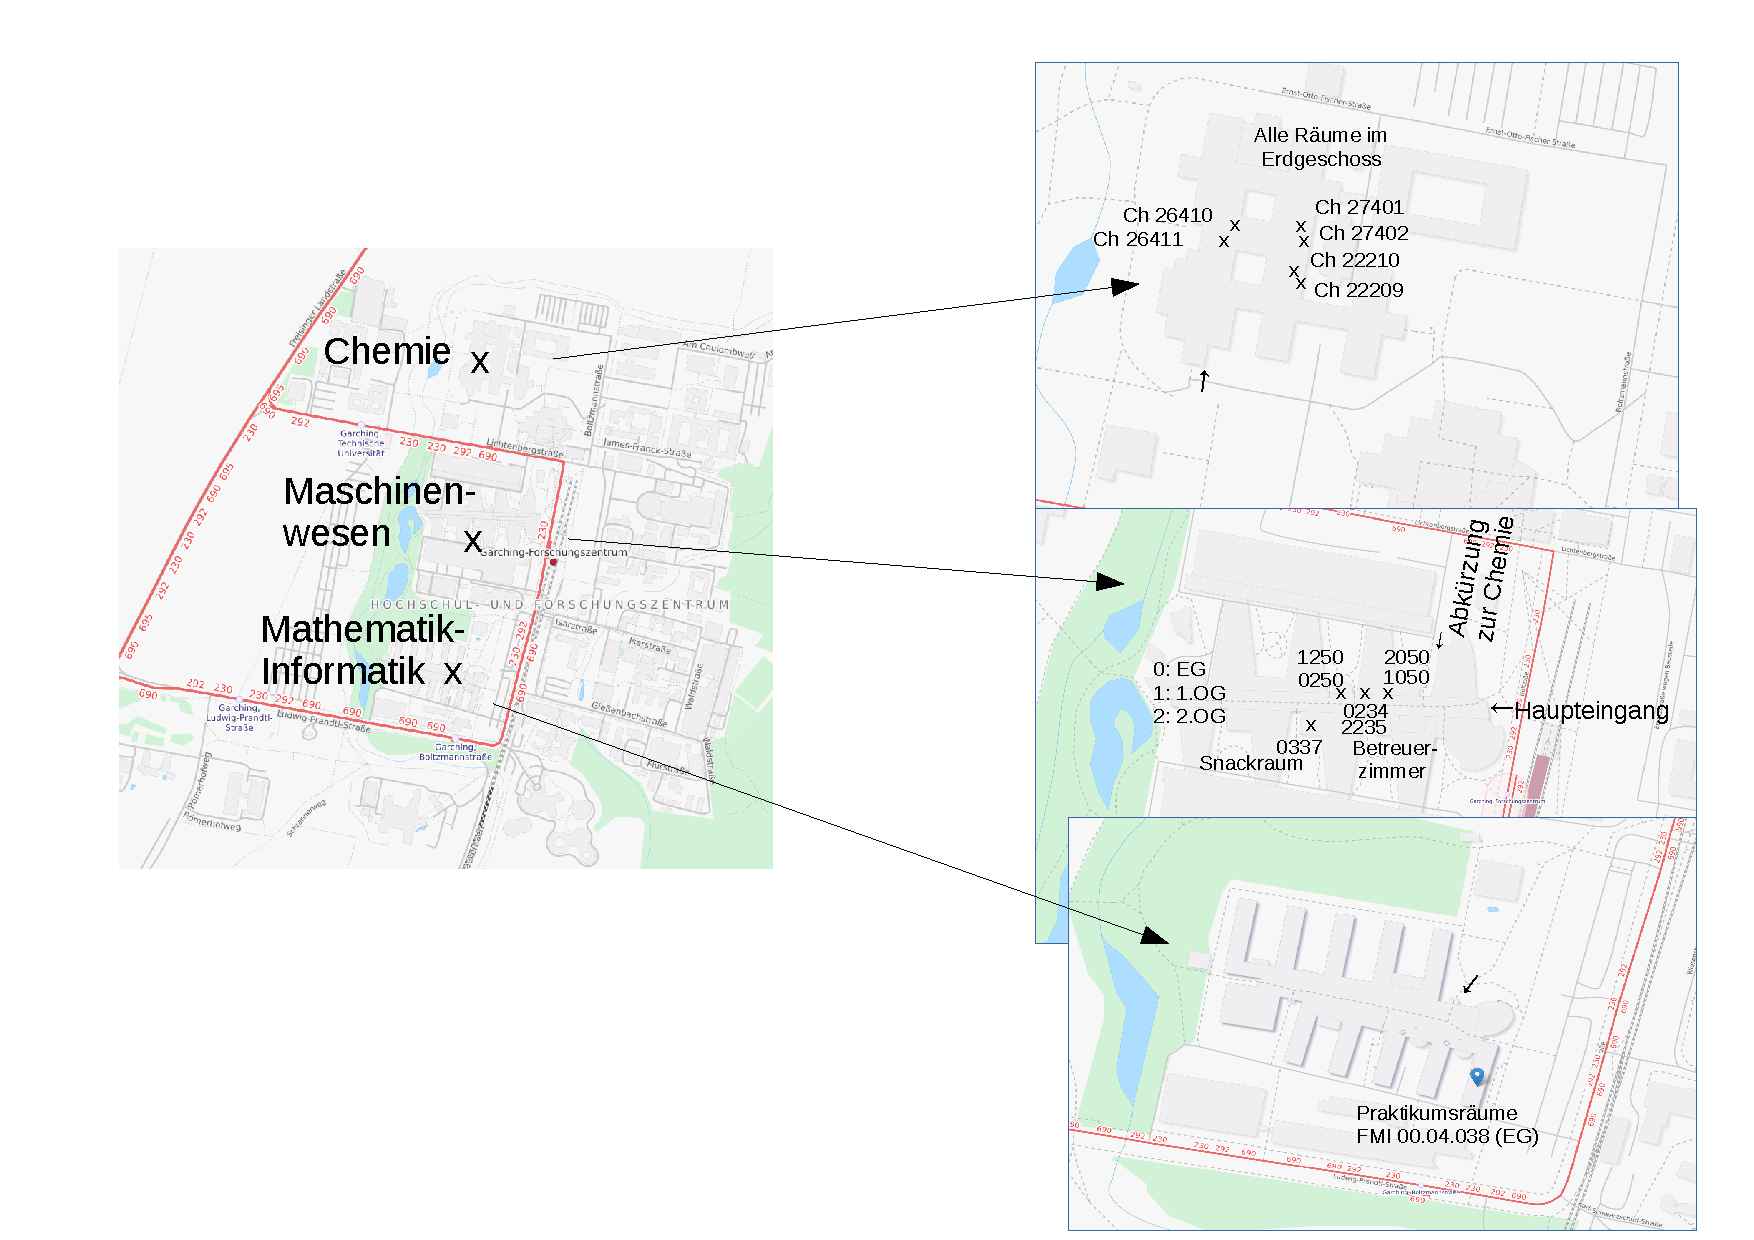
\includegraphics[scale=0.5]{campus_map.pdf}
\end{figure}
\newpage{}\begin{center}{\huge{}\textbf{Stundenplan von Alexis Michel}}\end{center}\textbf{{\large{}Donnerstag}}\nopagebreak \\\begin{tabular} {|p{3cm} p{6cm} p{6cm}| }\hline \textbf{11:30 bis 13:45}&\textbf{Anreise zur TU München}&\textbf{Fakultät Maschinenwesen}\\\hline \textbf{12:00 bis 13:30}&\textbf{Mittagessen}&\textbf{Mensa Garching}\\\hline \textbf{14:00}&\textbf{Begrüßung}&\textbf{CH 26411}\\&Begrüßung, Besprechung des Zeitplans, Ausgabe der individuellen Stundenpläne,...&\\\hline \textbf{14:50 bis 16:20}&\textbf{Thermodynamik 1}&\textbf{MW 1250}\\&Betreuer: Maximilian Marienhagen&ca. 12 Teilnehmer\\\hline \textbf{16:40 bis 18:10}&\textbf{Geometrische Optik}&\textbf{MW 0250}\\&Betreuer: Christopher Pfeiffer&ca. 13 Teilnehmer\\\hline \textbf{18:30}&\textbf{Fahrt zur Jugendherberge}&\textbf{}\\\hline \textbf{19:00}&\textbf{Abendessen}&\textbf{Jugendherberge}\\\hline \end{tabular}\\\vspace{5.00000mm}~\\\textbf{{\large{}Freitag}}\nopagebreak \\\begin{tabular} {|p{3cm} p{6cm} p{6cm}| }\hline \textbf{06:30 bis 09:00}&\textbf{Frühstück}&\textbf{Jugendherberge}\\\hline \textbf{09:00 bis 13:00}&frei&\\\hline \textbf{13:00 bis 14:00}&\textbf{Mittagessen}&\textbf{Mensa Garching}\\\hline \textbf{14:20 bis 15:50}&\textbf{Gewöhnliche Differentialgleichungen}&\textbf{MW 1250}\\&Betreuer: Sven Jandura&ca. 20 Teilnehmer\\\hline \textbf{16:10 bis 17:40}&\textbf{Experiment Oszilloskop}&\textbf{Praktikum Oszilloskop}\\&Betreuer: Christopher Pfeiffer&ca. 6 Teilnehmer\\\hline \textbf{18:00 bis 18:20}&\textbf{Erlebnisbericht IPhO}&\textbf{CH 26411}\\\hline \textbf{18:30}&\textbf{Fahrt zur Jugendherberge}&\textbf{}\\\hline \textbf{19:00}&\textbf{Abendessen}&\textbf{Jugendherberge}\\\hline \end{tabular}\\\vspace{5.00000mm}~\\\textbf{{\large{}Samstag}}\nopagebreak \\\begin{tabular} {|p{3cm} p{6cm} p{6cm}| }\hline \textbf{06:30 bis 08:00}&\textbf{Frühstück}&\textbf{Jugendherberge}\\\hline \textbf{08:00}&\textbf{Fahrt zur TU}&\textbf{}\\\hline \textbf{09:00 bis 10:30}&\textbf{Harmonische Schwingungen}&\textbf{MW 0250}\\&Betreuer: Ilja Göthel&ca. 9 Teilnehmer\\\hline \textbf{10:50 bis 12:20}&\textbf{Quanten- und Atomphysik I}&\textbf{MW 2050}\\&Betreuer: Vitaly Andreev&ca. 13 Teilnehmer\\\hline \textbf{12:40 bis 14:00}&\textbf{Mittagessen}&\textbf{Fakultät Maschinenwesen}\\\hline \textbf{14:20 bis 15:50}&\textbf{Relativistische Teilchenphysik}&\textbf{CH 22210}\\&Betreuer: Lars Dehlwes&ca. 23 Teilnehmer\\\hline \textbf{16:10 bis 17:40}&\textbf{Quanten- und Atomphysik II}&\textbf{CH 22209}\\&Betreuer: Vitaly Andreev&ca. 28 Teilnehmer\\\hline \textbf{18:00 bis 18:20}&\textbf{Vorstellung GYPT}&\textbf{CH 26411}\\\hline \textbf{18:30}&\textbf{Fahrt zur Jugendherberge}&\textbf{}\\\hline \textbf{19:00}&\textbf{Abendessen}&\textbf{Jugendherberge}\\\hline \end{tabular}\\\vspace{5.00000mm}~\\\textbf{{\large{}Sonntag}}\nopagebreak \\\begin{tabular} {|p{3cm} p{6cm} p{6cm}| }\hline \textbf{06:30 bis 08:00}&\textbf{Frühstück}&\textbf{Jugendherberge}\\\hline \textbf{08:00}&\textbf{Fahrt zur TU}&\textbf{}\\\hline \textbf{09:00 bis 10:30}&\textbf{Theoretische Mechanik}&\textbf{CH 22210}\\&Betreuer: Eugen Dizer&ca. 13 Teilnehmer\\\hline \textbf{10:50 bis 12:20}&\textbf{Wellenoptik}&\textbf{MW 0250}\\&Betreuer: Christopher Pfeiffer&ca. 12 Teilnehmer\\\hline \textbf{12:40 bis 13:00}&\textbf{Verabschiedung}&\textbf{CH 26411}\\\hline \textbf{13:00}&\textbf{Individuelle Abreise}&\textbf{}\\\hline \textbf{13:00 bis 14:00}&\textbf{Mittagessen}&\textbf{}\\\hline \end{tabular}\\\vspace{5.00000mm}~\\
Notfallnummern: \\
Sven Jandura: xxxx xxxxxxxxx \\
Johannes Rothe: xxxx xxxxxxxxx \\

\large Hast du Lust, die Andern vom Seminar wiederzusehen?\\
\normalsize Dann komm doch einfach zum \textbf{Vereinstreffen}. Dazu musst du kein Vereinsmitglied sein. Neben interesannten Vorträgen und Exkursionen sind jede Menge Spiel und Spaß geplant. Schau in einem Monat einfach noch mal auf der Website vorbei. Wir freuen uns, wenn du dabei bist.

\begin{figure}[!h]
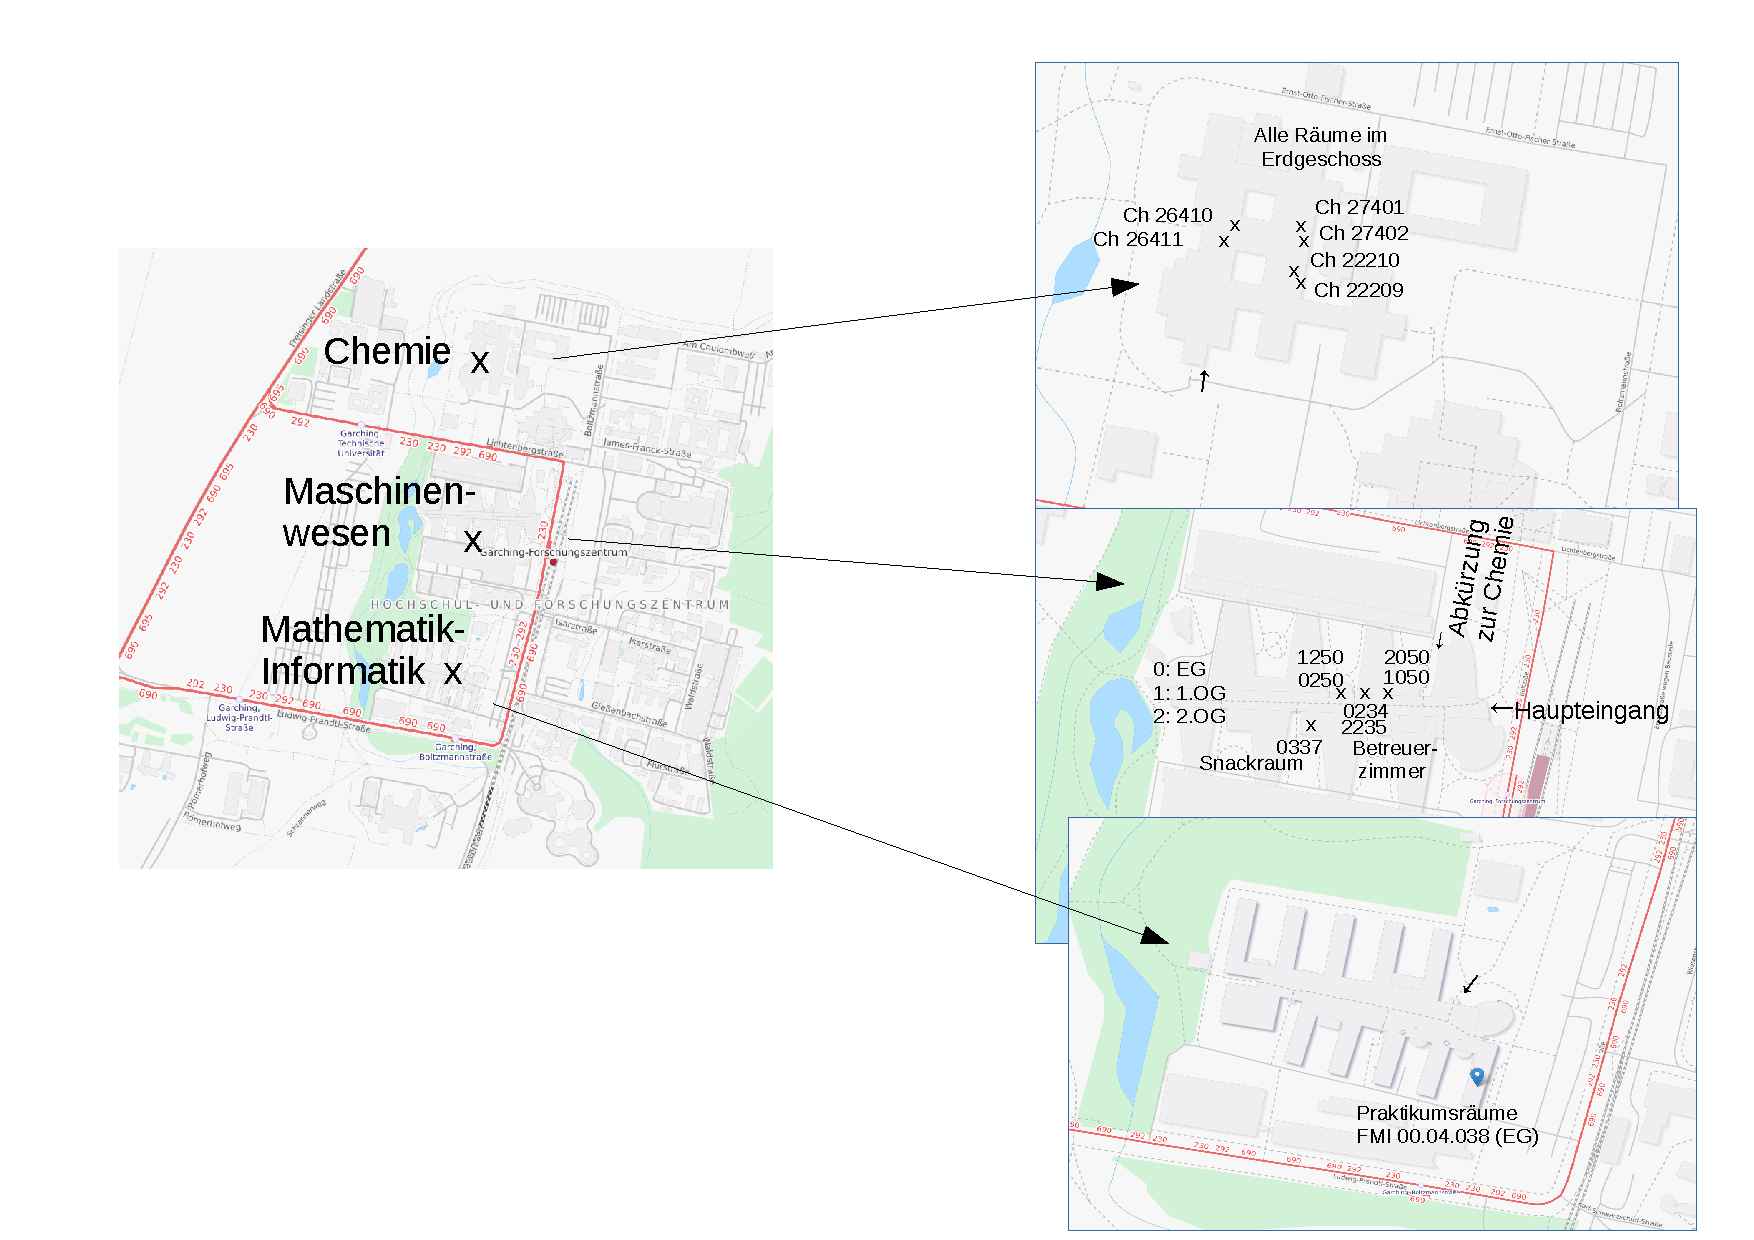
\includegraphics[scale=0.5]{campus_map.pdf}
\end{figure}
\newpage{}\begin{center}{\huge{}\textbf{Stundenplan von Amelie Birli}}\end{center}\textbf{{\large{}Donnerstag}}\nopagebreak \\\begin{tabular} {|p{3cm} p{6cm} p{6cm}| }\hline \textbf{11:30 bis 13:45}&\textbf{Anreise zur TU München}&\textbf{Fakultät Maschinenwesen}\\\hline \textbf{12:00 bis 13:30}&\textbf{Mittagessen}&\textbf{Mensa Garching}\\\hline \textbf{14:00}&\textbf{Begrüßung}&\textbf{CH 26411}\\&Begrüßung, Besprechung des Zeitplans, Ausgabe der individuellen Stundenpläne,...&\\\hline \textbf{14:50 bis 16:20}&\textbf{Quanten- und Atomphysik I}&\textbf{CH 26410}\\&Betreuer: Ismail Achmed-Zade&ca. 28 Teilnehmer\\\hline \textbf{16:40 bis 18:10}&\textbf{Näherungsmethoden}&\textbf{MW 0234}\\&Betreuer: Ilja Göthel&ca. 13 Teilnehmer\\\hline \textbf{18:30}&\textbf{Fahrt zur Jugendherberge}&\textbf{}\\\hline \textbf{19:00}&\textbf{Abendessen}&\textbf{Jugendherberge}\\\hline \end{tabular}\\\vspace{5.00000mm}~\\\textbf{{\large{}Freitag}}\nopagebreak \\\begin{tabular} {|p{3cm} p{6cm} p{6cm}| }\hline \textbf{06:30 bis 09:00}&\textbf{Frühstück}&\textbf{Jugendherberge}\\\hline \textbf{09:00 bis 13:00}&\textbf{Besichtigung der Forschungsneutronenquelle FRM II}&\textbf{MW 2050}\\&Betreuer: Felix Wechsler&ca. 28 Teilnehmer\\\hline \textbf{13:00 bis 14:00}&\textbf{Mittagessen}&\textbf{Mensa Garching}\\\hline \textbf{14:20 bis 15:50}&\textbf{Gewöhnliche Differentialgleichungen}&\textbf{MW 1250}\\&Betreuer: Sven Jandura&ca. 20 Teilnehmer\\\hline \textbf{16:10 bis 17:40}&\textbf{Harmonische Schwingungen}&\textbf{MW 2050}\\&Betreuer: Ilja Göthel&ca. 3 Teilnehmer\\\hline \textbf{18:00 bis 18:20}&\textbf{Erlebnisbericht IPhO}&\textbf{CH 26411}\\\hline \textbf{18:30}&\textbf{Fahrt zur Jugendherberge}&\textbf{}\\\hline \textbf{19:00}&\textbf{Abendessen}&\textbf{Jugendherberge}\\\hline \end{tabular}\\\vspace{5.00000mm}~\\\textbf{{\large{}Samstag}}\nopagebreak \\\begin{tabular} {|p{3cm} p{6cm} p{6cm}| }\hline \textbf{06:30 bis 08:00}&\textbf{Frühstück}&\textbf{Jugendherberge}\\\hline \textbf{08:00}&\textbf{Fahrt zur TU}&\textbf{}\\\hline \textbf{09:00 bis 10:30}&\textbf{Elektrodynamik 1}&\textbf{MW 1250}\\&Betreuer: Maximilian Keitel&ca. 21 Teilnehmer\\\hline \textbf{10:50 bis 12:20}&\textbf{Elektrodynamik 2}&\textbf{MW 1250}\\&Betreuer: Maximilian Keitel&ca. 21 Teilnehmer\\\hline \textbf{12:40 bis 14:00}&\textbf{Mittagessen}&\textbf{Fakultät Maschinenwesen}\\\hline \textbf{14:20 bis 15:50}&\textbf{Relativistische Teilchenphysik}&\textbf{CH 22210}\\&Betreuer: Lars Dehlwes&ca. 23 Teilnehmer\\\hline \textbf{16:10 bis 17:40}&\textbf{Quanten- und Atomphysik II}&\textbf{CH 22209}\\&Betreuer: Vitaly Andreev&ca. 28 Teilnehmer\\\hline \textbf{18:00 bis 18:20}&\textbf{Vorstellung GYPT}&\textbf{CH 26411}\\\hline \textbf{18:30}&\textbf{Fahrt zur Jugendherberge}&\textbf{}\\\hline \textbf{19:00}&\textbf{Abendessen}&\textbf{Jugendherberge}\\\hline \end{tabular}\\\vspace{5.00000mm}~\\\textbf{{\large{}Sonntag}}\nopagebreak \\\begin{tabular} {|p{3cm} p{6cm} p{6cm}| }\hline \textbf{06:30 bis 08:00}&\textbf{Frühstück}&\textbf{Jugendherberge}\\\hline \textbf{08:00}&\textbf{Fahrt zur TU}&\textbf{}\\\hline \textbf{09:00 bis 10:30}&\textbf{Aufgabenseminar Elektrodynamik}&\textbf{MW 0234}\\&Betreuer: Maximilian Keitel&ca. 4 Teilnehmer\\\hline \textbf{10:50 bis 12:20}&\textbf{Aufgabenseminar Quanten- und Atomphysik und Struktur der Materie}&\textbf{MW 1250}\\&Betreuer: Vitaly Andreev&ca. 24 Teilnehmer\\\hline \textbf{12:40 bis 13:00}&\textbf{Verabschiedung}&\textbf{CH 26411}\\\hline \textbf{13:00}&\textbf{Individuelle Abreise}&\textbf{}\\\hline \textbf{13:00 bis 14:00}&\textbf{Mittagessen}&\textbf{}\\\hline \end{tabular}\\\vspace{5.00000mm}~\\
Notfallnummern: \\
Sven Jandura: xxxx xxxxxxxxx \\
Johannes Rothe: xxxx xxxxxxxxx \\

\large Hast du Lust, die Andern vom Seminar wiederzusehen?\\
\normalsize Dann komm doch einfach zum \textbf{Vereinstreffen}. Dazu musst du kein Vereinsmitglied sein. Neben interesannten Vorträgen und Exkursionen sind jede Menge Spiel und Spaß geplant. Schau in einem Monat einfach noch mal auf der Website vorbei. Wir freuen uns, wenn du dabei bist.

\begin{figure}[!h]
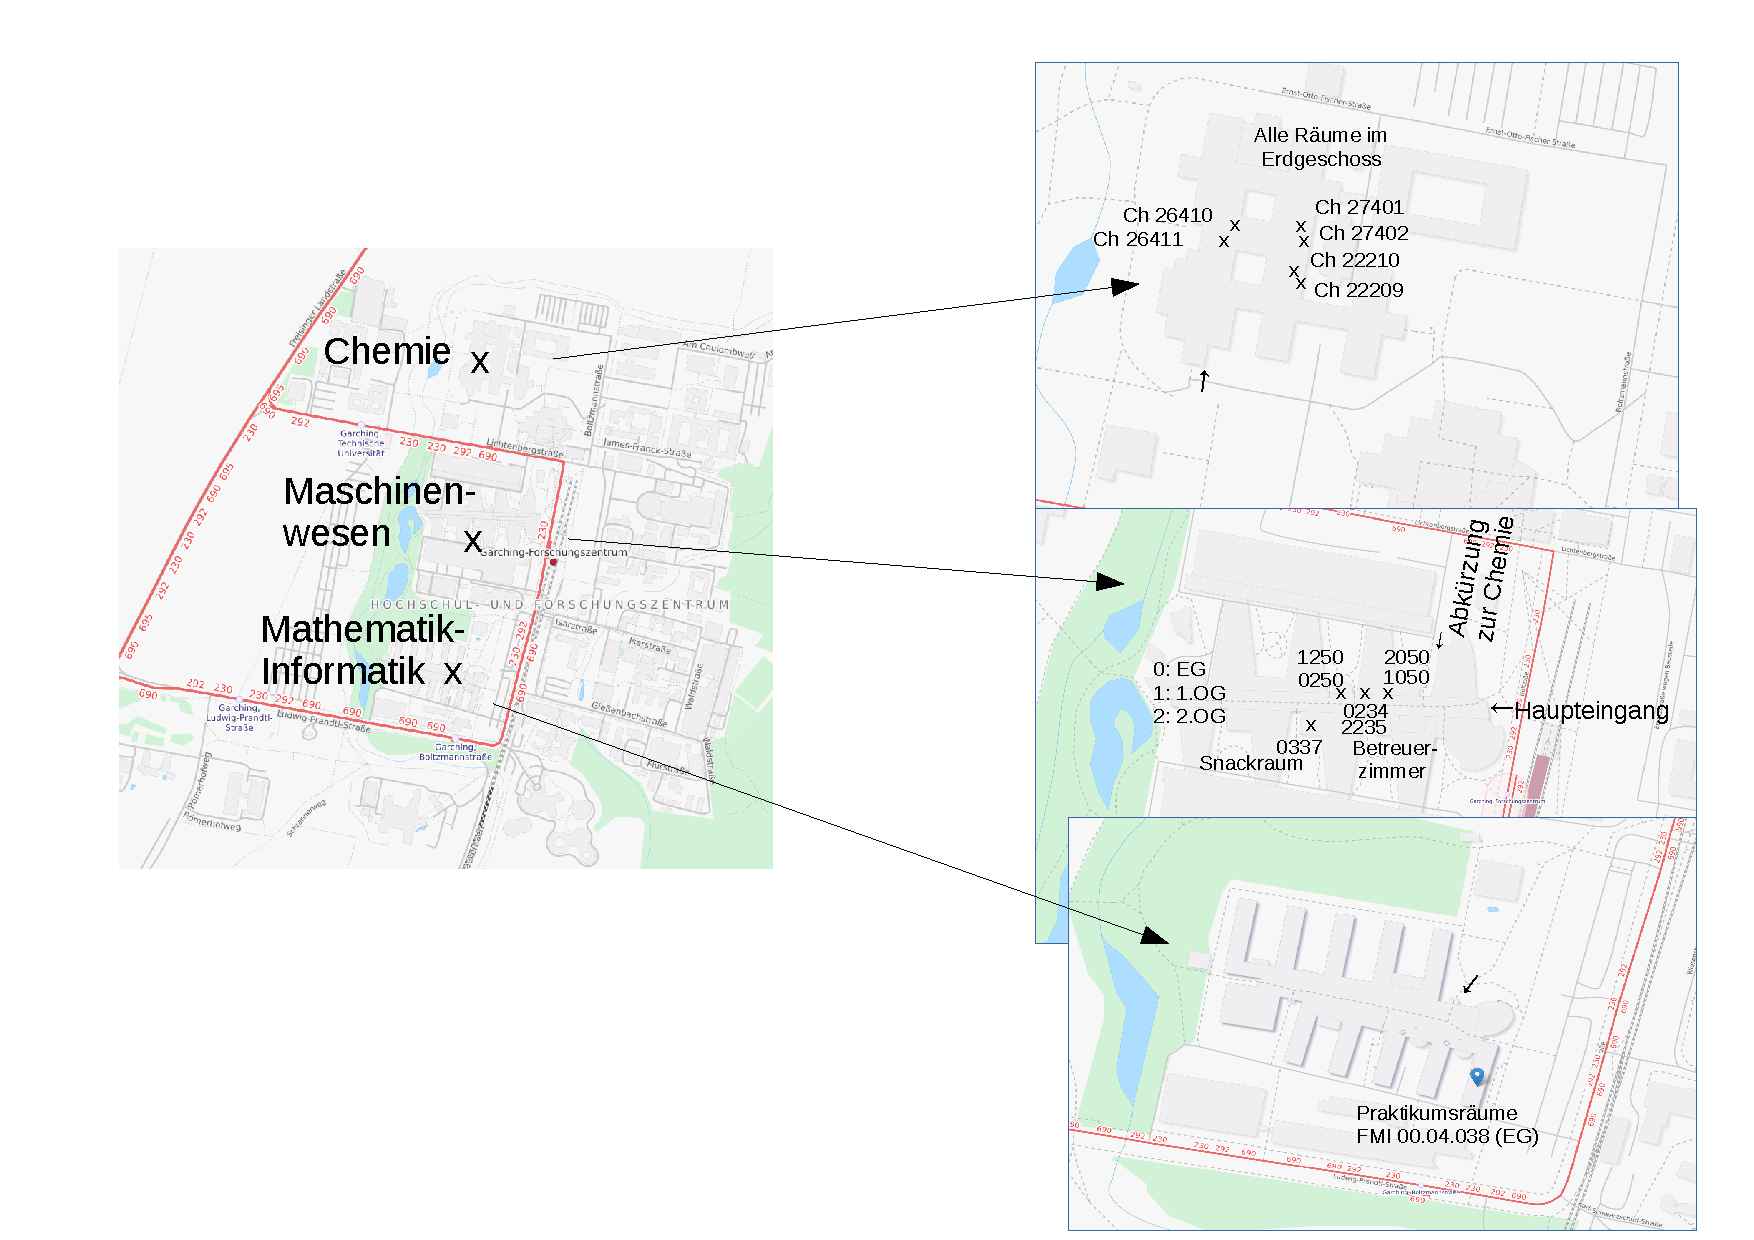
\includegraphics[scale=0.5]{campus_map.pdf}
\end{figure}
\newpage{}\begin{center}{\huge{}\textbf{Stundenplan von Anja Hoffmeister}}\end{center}\textbf{{\large{}Donnerstag}}\nopagebreak \\\begin{tabular} {|p{3cm} p{6cm} p{6cm}| }\hline \textbf{11:30 bis 13:45}&\textbf{Anreise zur TU München}&\textbf{Fakultät Maschinenwesen}\\\hline \textbf{12:00 bis 13:30}&\textbf{Mittagessen}&\textbf{Mensa Garching}\\\hline \textbf{14:00}&\textbf{Begrüßung}&\textbf{CH 26411}\\&Begrüßung, Besprechung des Zeitplans, Ausgabe der individuellen Stundenpläne,...&\\\hline \textbf{14:50 bis 16:20}&\textbf{Experimentieren und Auswerten}&\textbf{CH 26411}\\&Betreuer: Ann-Kathrin Raab&ca. 18 Teilnehmer\\\hline \textbf{16:40 bis 18:10}&\textbf{Geometrische Optik}&\textbf{MW 0250}\\&Betreuer: Christopher Pfeiffer&ca. 13 Teilnehmer\\\hline \textbf{18:30}&\textbf{Fahrt zur Jugendherberge}&\textbf{}\\\hline \textbf{19:00}&\textbf{Abendessen}&\textbf{Jugendherberge}\\\hline \end{tabular}\\\vspace{5.00000mm}~\\\textbf{{\large{}Freitag}}\nopagebreak \\\begin{tabular} {|p{3cm} p{6cm} p{6cm}| }\hline \textbf{06:30 bis 09:00}&\textbf{Frühstück}&\textbf{Jugendherberge}\\\hline \textbf{09:00 bis 13:00}&frei&\\\hline \textbf{13:00 bis 14:00}&\textbf{Mittagessen}&\textbf{Mensa Garching}\\\hline \textbf{14:20 bis 15:50}&\textbf{Experiment spezifische Elektronenladung}&\textbf{Praktikum spezifische Elektronenladung}\\&Betreuer: Felix Wechsler&ca. 6 Teilnehmer\\\hline \textbf{16:10 bis 17:40}&\textbf{Spezielle Relativitätstheorie}&\textbf{MW 1250}\\&Betreuer: Johannes Rothe&ca. 19 Teilnehmer\\\hline \textbf{18:00 bis 18:20}&\textbf{Erlebnisbericht IPhO}&\textbf{CH 26411}\\\hline \textbf{18:30}&\textbf{Fahrt zur Jugendherberge}&\textbf{}\\\hline \textbf{19:00}&\textbf{Abendessen}&\textbf{Jugendherberge}\\\hline \end{tabular}\\\vspace{5.00000mm}~\\\textbf{{\large{}Samstag}}\nopagebreak \\\begin{tabular} {|p{3cm} p{6cm} p{6cm}| }\hline \textbf{06:30 bis 08:00}&\textbf{Frühstück}&\textbf{Jugendherberge}\\\hline \textbf{08:00}&\textbf{Fahrt zur TU}&\textbf{}\\\hline \textbf{09:00 bis 10:30}&\textbf{Experiment Millikan-Versuch}&\textbf{Praktikum Millikan-Versuch}\\&Betreuer: Samuel Moll&ca. 6 Teilnehmer\\\hline \textbf{10:50 bis 12:20}&\textbf{Experiment Reversionspendel}&\textbf{Praktikum Reversionspendel}\\&Betreuer: Lilith Diringer&ca. 6 Teilnehmer\\\hline \textbf{12:40 bis 14:00}&\textbf{Mittagessen}&\textbf{Fakultät Maschinenwesen}\\\hline \textbf{14:20 bis 15:50}&\textbf{Quanten- und Atomphysik I}&\textbf{CH 22209}\\&Betreuer: Vitaly Andreev&ca. 22 Teilnehmer\\\hline \textbf{16:10 bis 17:40}&\textbf{Quanten- und Atomphysik II}&\textbf{CH 22209}\\&Betreuer: Vitaly Andreev&ca. 28 Teilnehmer\\\hline \textbf{18:00 bis 18:20}&\textbf{Vorstellung GYPT}&\textbf{CH 26411}\\\hline \textbf{18:30}&\textbf{Fahrt zur Jugendherberge}&\textbf{}\\\hline \textbf{19:00}&\textbf{Abendessen}&\textbf{Jugendherberge}\\\hline \end{tabular}\\\vspace{5.00000mm}~\\\textbf{{\large{}Sonntag}}\nopagebreak \\\begin{tabular} {|p{3cm} p{6cm} p{6cm}| }\hline \textbf{06:30 bis 08:00}&\textbf{Frühstück}&\textbf{Jugendherberge}\\\hline \textbf{08:00}&\textbf{Fahrt zur TU}&\textbf{}\\\hline \textbf{09:00 bis 10:30}&\textbf{Gravitationsbeschleunigung}&\textbf{MW 1050}\\&Betreuer: Ann-Kathrin Raab&ca. 8 Teilnehmer\\\hline \textbf{10:50 bis 12:20}&\textbf{Wellenoptik}&\textbf{MW 0250}\\&Betreuer: Christopher Pfeiffer&ca. 12 Teilnehmer\\\hline \textbf{12:40 bis 13:00}&\textbf{Verabschiedung}&\textbf{CH 26411}\\\hline \textbf{13:00}&\textbf{Individuelle Abreise}&\textbf{}\\\hline \textbf{13:00 bis 14:00}&\textbf{Mittagessen}&\textbf{}\\\hline \end{tabular}\\\vspace{5.00000mm}~\\
Notfallnummern: \\
Sven Jandura: xxxx xxxxxxxxx \\
Johannes Rothe: xxxx xxxxxxxxx \\

\large Hast du Lust, die Andern vom Seminar wiederzusehen?\\
\normalsize Dann komm doch einfach zum \textbf{Vereinstreffen}. Dazu musst du kein Vereinsmitglied sein. Neben interesannten Vorträgen und Exkursionen sind jede Menge Spiel und Spaß geplant. Schau in einem Monat einfach noch mal auf der Website vorbei. Wir freuen uns, wenn du dabei bist.

\begin{figure}[!h]
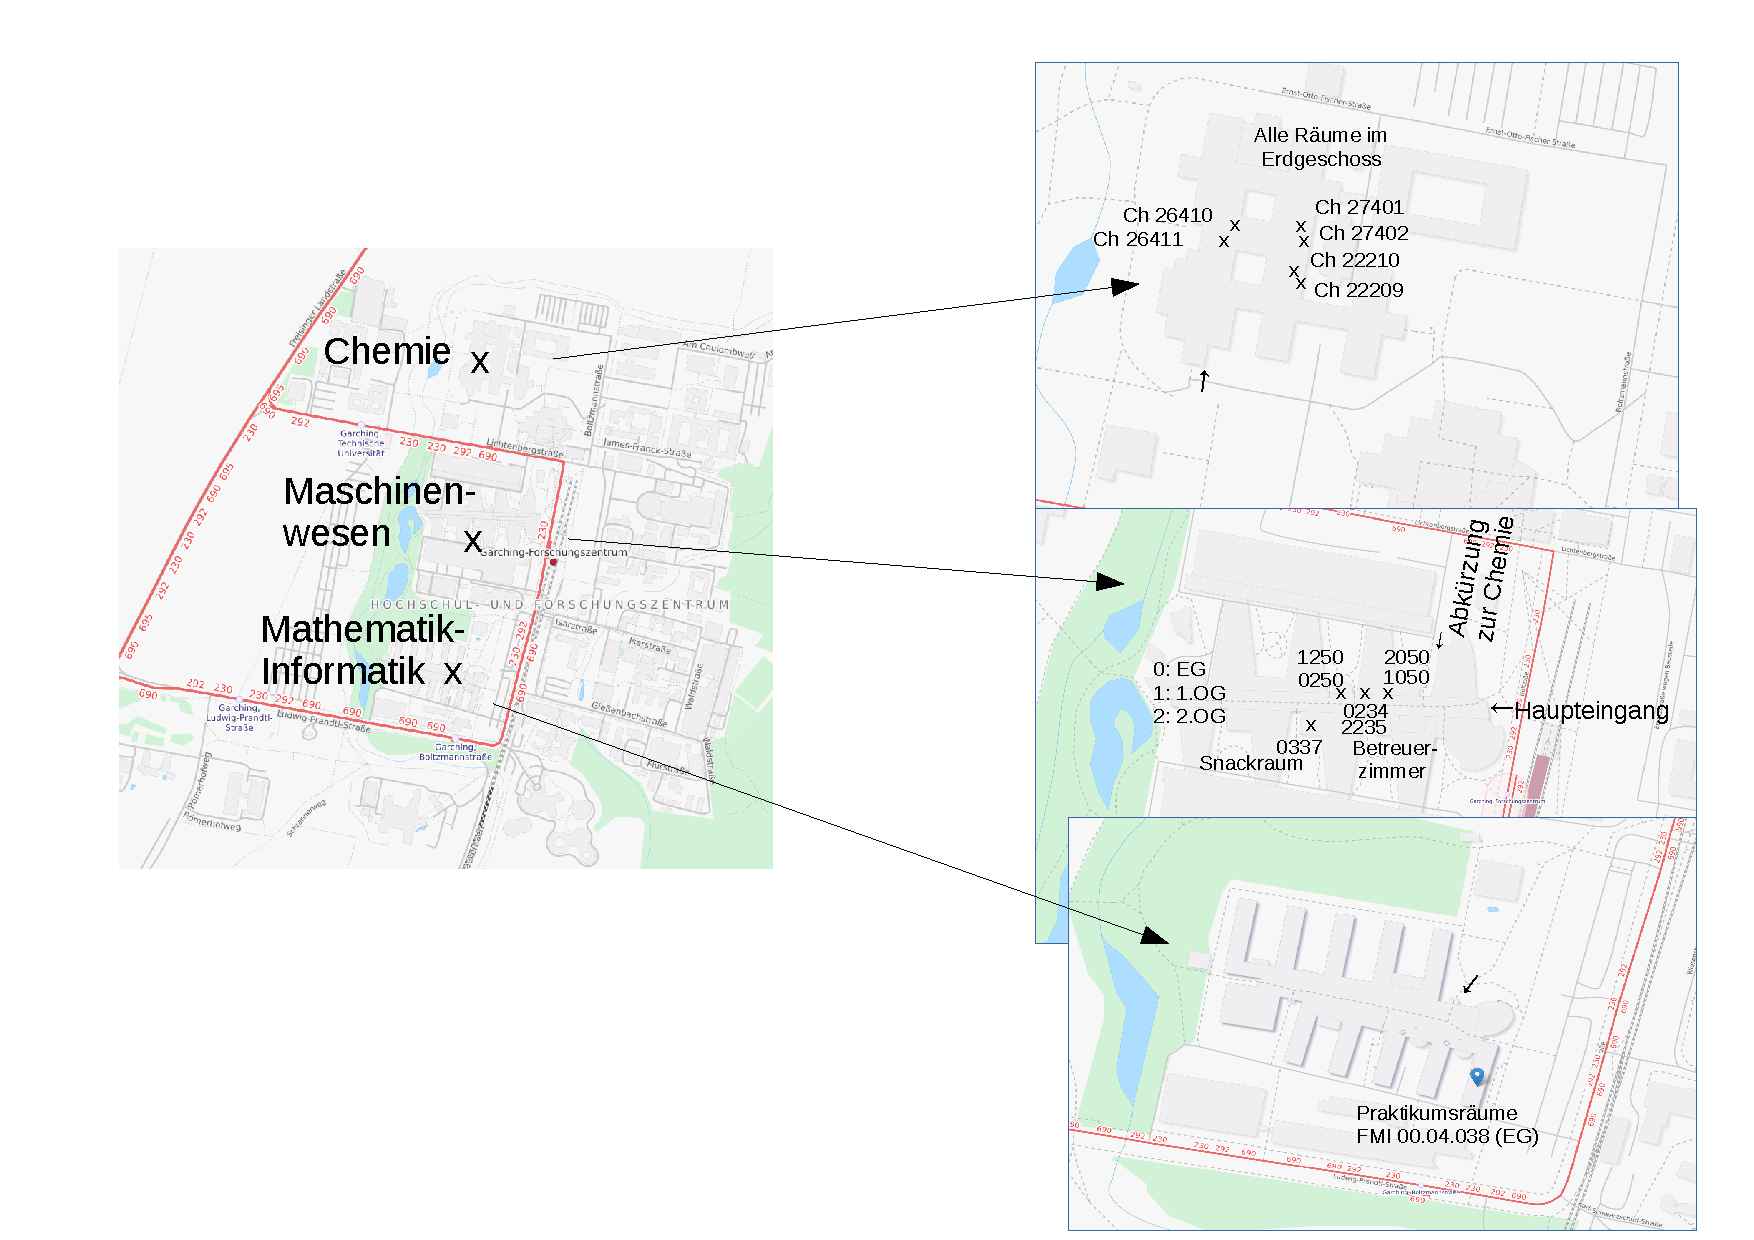
\includegraphics[scale=0.5]{campus_map.pdf}
\end{figure}
\newpage{}\begin{center}{\huge{}\textbf{Stundenplan von Anton Haas}}\end{center}\textbf{{\large{}Donnerstag}}\nopagebreak \\\begin{tabular} {|p{3cm} p{6cm} p{6cm}| }\hline \textbf{11:30 bis 13:45}&\textbf{Anreise zur TU München}&\textbf{Fakultät Maschinenwesen}\\\hline \textbf{12:00 bis 13:30}&\textbf{Mittagessen}&\textbf{Mensa Garching}\\\hline \textbf{14:00}&\textbf{Begrüßung}&\textbf{CH 26411}\\&Begrüßung, Besprechung des Zeitplans, Ausgabe der individuellen Stundenpläne,...&\\\hline \textbf{14:50 bis 16:20}&\textbf{Elektrische Schaltungen}&\textbf{MW 0250}\\&Betreuer: Christopher Pfeiffer&ca. 16 Teilnehmer\\\hline \textbf{16:40 bis 18:10}&\textbf{Experimentieren und Auswerten}&\textbf{CH 26411}\\&Betreuer: Ann-Kathrin Raab&ca. 15 Teilnehmer\\\hline \textbf{18:30}&\textbf{Fahrt zur Jugendherberge}&\textbf{}\\\hline \textbf{19:00}&\textbf{Abendessen}&\textbf{Jugendherberge}\\\hline \end{tabular}\\\vspace{5.00000mm}~\\\textbf{{\large{}Freitag}}\nopagebreak \\\begin{tabular} {|p{3cm} p{6cm} p{6cm}| }\hline \textbf{06:30 bis 09:00}&\textbf{Frühstück}&\textbf{Jugendherberge}\\\hline \textbf{09:00 bis 13:00}&frei&\\\hline \textbf{13:00 bis 14:00}&\textbf{Mittagessen}&\textbf{Mensa Garching}\\\hline \textbf{14:20 bis 15:50}&\textbf{Experiment Oszilloskop}&\textbf{Praktikum Oszilloskop}\\&Betreuer: Christopher Pfeiffer&ca. 6 Teilnehmer\\\hline \textbf{16:10 bis 17:40}&\textbf{Experiment Magnetismus}&\textbf{Praktikum Magnetismus}\\&Betreuer: Lars Dehlwes&ca. 6 Teilnehmer\\\hline \textbf{18:00 bis 18:20}&\textbf{Erlebnisbericht IPhO}&\textbf{CH 26411}\\\hline \textbf{18:30}&\textbf{Fahrt zur Jugendherberge}&\textbf{}\\\hline \textbf{19:00}&\textbf{Abendessen}&\textbf{Jugendherberge}\\\hline \end{tabular}\\\vspace{5.00000mm}~\\\textbf{{\large{}Samstag}}\nopagebreak \\\begin{tabular} {|p{3cm} p{6cm} p{6cm}| }\hline \textbf{06:30 bis 08:00}&\textbf{Frühstück}&\textbf{Jugendherberge}\\\hline \textbf{08:00}&\textbf{Fahrt zur TU}&\textbf{}\\\hline \textbf{09:00 bis 10:30}&\textbf{Harmonische Schwingungen}&\textbf{MW 0250}\\&Betreuer: Ilja Göthel&ca. 9 Teilnehmer\\\hline \textbf{10:50 bis 12:20}&\textbf{Klassische Mechanik}&\textbf{MW 1050}\\&Betreuer: Maximilian Marienhagen&ca. 3 Teilnehmer\\\hline \textbf{12:40 bis 14:00}&\textbf{Mittagessen}&\textbf{Fakultät Maschinenwesen}\\\hline \textbf{14:20 bis 15:50}&\textbf{Bestimmung des Brechungskoeffizienten von Plexiglas}&\textbf{MW 0234}\\&Betreuer: Lilith Diringer&ca. 8 Teilnehmer\\\hline \textbf{16:10 bis 17:40}&\textbf{Bestimmung des Brechungskoeffizienten von Wasser}&\textbf{MW 0234}\\&Betreuer: Lilith Diringer&ca. 8 Teilnehmer\\\hline \textbf{18:00 bis 18:20}&\textbf{Vorstellung GYPT}&\textbf{CH 26411}\\\hline \textbf{18:30}&\textbf{Fahrt zur Jugendherberge}&\textbf{}\\\hline \textbf{19:00}&\textbf{Abendessen}&\textbf{Jugendherberge}\\\hline \end{tabular}\\\vspace{5.00000mm}~\\\textbf{{\large{}Sonntag}}\nopagebreak \\\begin{tabular} {|p{3cm} p{6cm} p{6cm}| }\hline \textbf{06:30 bis 08:00}&\textbf{Frühstück}&\textbf{Jugendherberge}\\\hline \textbf{08:00}&\textbf{Fahrt zur TU}&\textbf{}\\\hline \textbf{09:00 bis 10:30}&\textbf{Gravitationsbeschleunigung}&\textbf{MW 1050}\\&Betreuer: Ann-Kathrin Raab&ca. 8 Teilnehmer\\\hline \textbf{10:50 bis 12:20}&\textbf{Rotationsbewegungen}&\textbf{CH 26410}\\&Betreuer: Vincent Grande&ca. 9 Teilnehmer\\\hline \textbf{12:40 bis 13:00}&\textbf{Verabschiedung}&\textbf{CH 26411}\\\hline \textbf{13:00}&\textbf{Individuelle Abreise}&\textbf{}\\\hline \textbf{13:00 bis 14:00}&\textbf{Mittagessen}&\textbf{}\\\hline \end{tabular}\\\vspace{5.00000mm}~\\
Notfallnummern: \\
Sven Jandura: xxxx xxxxxxxxx \\
Johannes Rothe: xxxx xxxxxxxxx \\

\large Hast du Lust, die Andern vom Seminar wiederzusehen?\\
\normalsize Dann komm doch einfach zum \textbf{Vereinstreffen}. Dazu musst du kein Vereinsmitglied sein. Neben interesannten Vorträgen und Exkursionen sind jede Menge Spiel und Spaß geplant. Schau in einem Monat einfach noch mal auf der Website vorbei. Wir freuen uns, wenn du dabei bist.

\begin{figure}[!h]
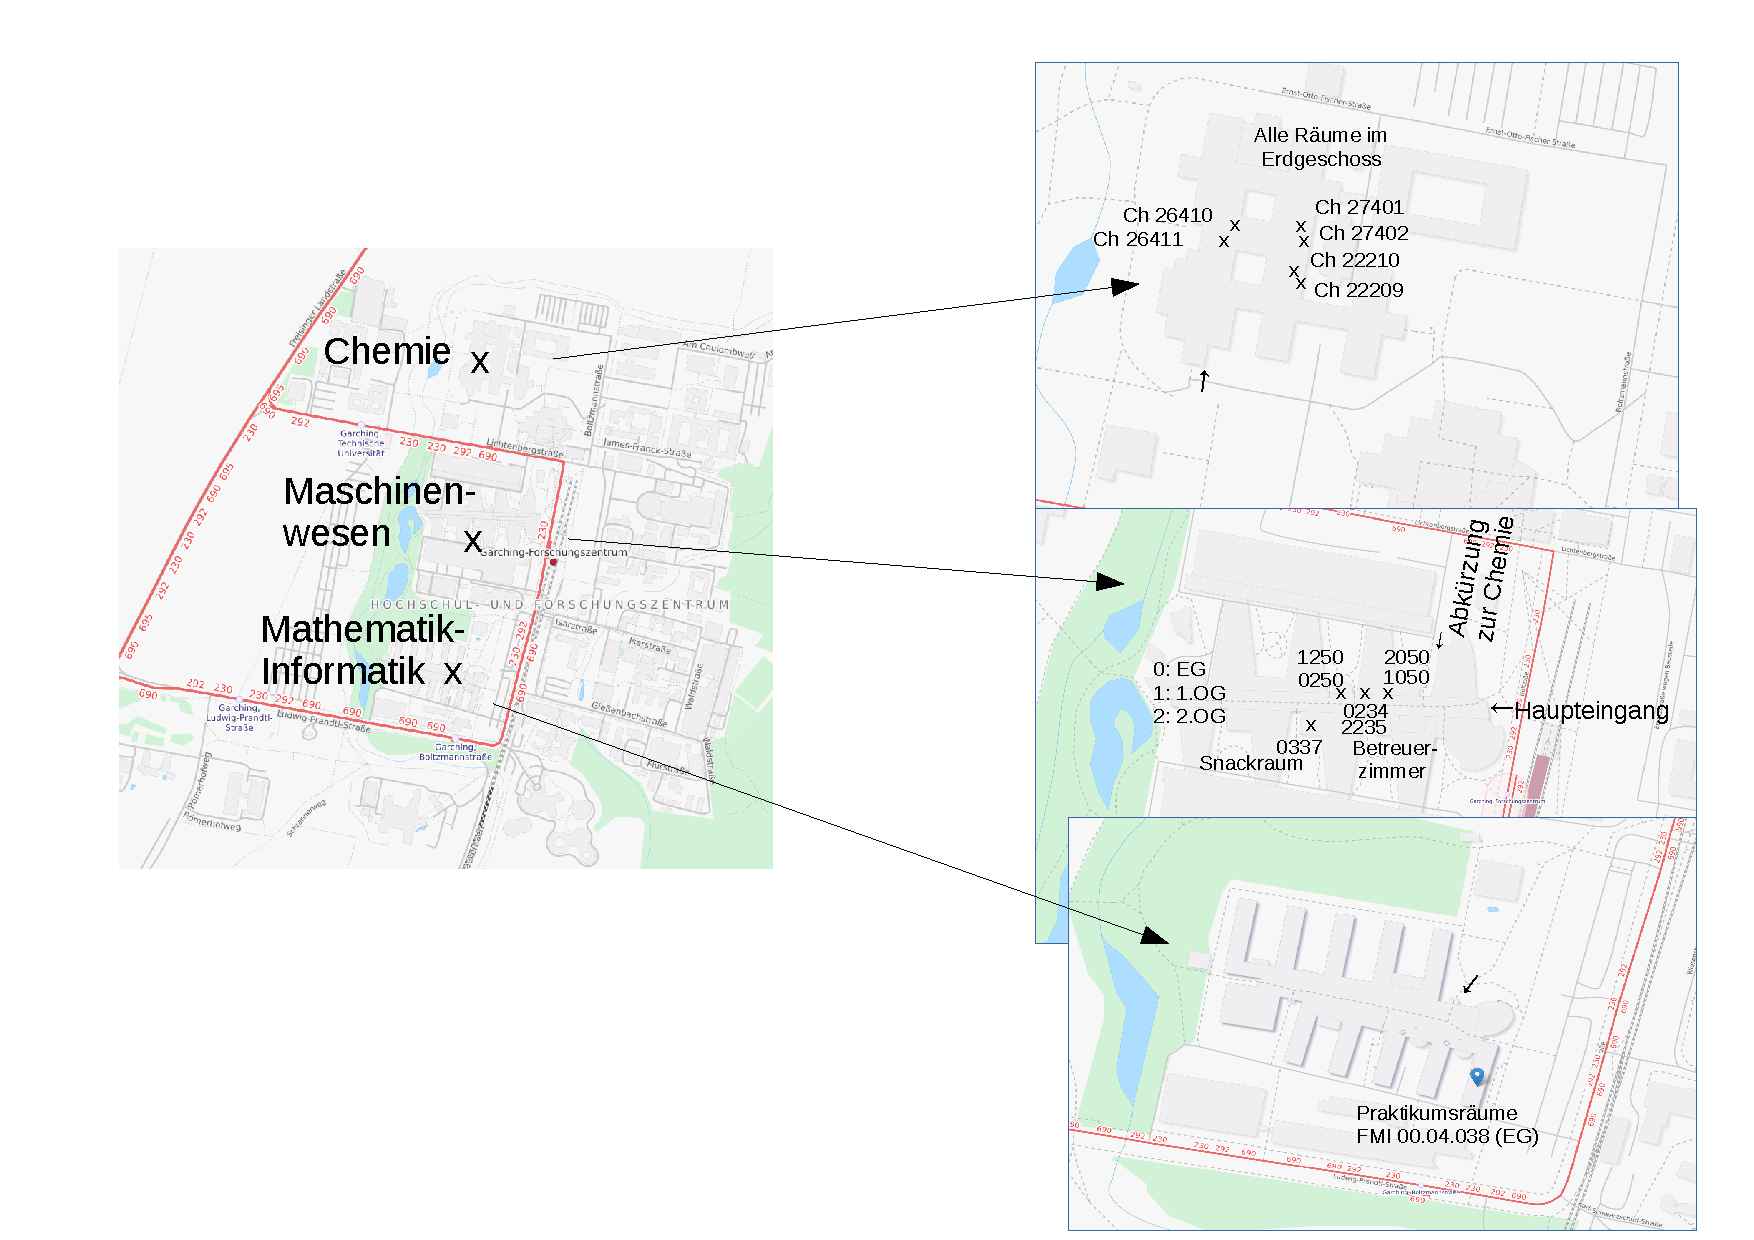
\includegraphics[scale=0.5]{campus_map.pdf}
\end{figure}
\newpage{}\begin{center}{\huge{}\textbf{Stundenplan von Antonia Westphal}}\end{center}\textbf{{\large{}Donnerstag}}\nopagebreak \\\begin{tabular} {|p{3cm} p{6cm} p{6cm}| }\hline \textbf{11:30 bis 13:45}&\textbf{Anreise zur TU München}&\textbf{Fakultät Maschinenwesen}\\\hline \textbf{12:00 bis 13:30}&\textbf{Mittagessen}&\textbf{Mensa Garching}\\\hline \textbf{14:00}&\textbf{Begrüßung}&\textbf{CH 26411}\\&Begrüßung, Besprechung des Zeitplans, Ausgabe der individuellen Stundenpläne,...&\\\hline \textbf{14:50 bis 16:20}&\textbf{Experimentieren und Auswerten}&\textbf{CH 26411}\\&Betreuer: Ann-Kathrin Raab&ca. 18 Teilnehmer\\\hline \textbf{16:40 bis 18:10}&\textbf{Einführung ins Integrieren}&\textbf{MW 1050}\\&Betreuer: Johannes Rothe&ca. 14 Teilnehmer\\\hline \textbf{18:30}&\textbf{Fahrt zur Jugendherberge}&\textbf{}\\\hline \textbf{19:00}&\textbf{Abendessen}&\textbf{Jugendherberge}\\\hline \end{tabular}\\\vspace{5.00000mm}~\\\textbf{{\large{}Freitag}}\nopagebreak \\\begin{tabular} {|p{3cm} p{6cm} p{6cm}| }\hline \textbf{06:30 bis 09:00}&\textbf{Frühstück}&\textbf{Jugendherberge}\\\hline \textbf{09:00 bis 13:00}&\textbf{Besichtigung der Forschungsneutronenquelle FRM II}&\textbf{MW 2050}\\&Betreuer: Felix Wechsler&ca. 28 Teilnehmer\\\hline \textbf{13:00 bis 14:00}&\textbf{Mittagessen}&\textbf{Mensa Garching}\\\hline \textbf{14:20 bis 15:50}&\textbf{Kernphysik}&\textbf{MW 0250}\\&Betreuer: Johannes Rothe&ca. 18 Teilnehmer\\\hline \textbf{16:10 bis 17:40}&\textbf{Spezielle Relativitätstheorie}&\textbf{MW 1250}\\&Betreuer: Johannes Rothe&ca. 19 Teilnehmer\\\hline \textbf{18:00 bis 18:20}&\textbf{Erlebnisbericht IPhO}&\textbf{CH 26411}\\\hline \textbf{18:30}&\textbf{Fahrt zur Jugendherberge}&\textbf{}\\\hline \textbf{19:00}&\textbf{Abendessen}&\textbf{Jugendherberge}\\\hline \end{tabular}\\\vspace{5.00000mm}~\\\textbf{{\large{}Samstag}}\nopagebreak \\\begin{tabular} {|p{3cm} p{6cm} p{6cm}| }\hline \textbf{06:30 bis 08:00}&\textbf{Frühstück}&\textbf{Jugendherberge}\\\hline \textbf{08:00}&\textbf{Fahrt zur TU}&\textbf{}\\\hline \textbf{09:00 bis 10:30}&\textbf{Elektrodynamik 1}&\textbf{MW 1250}\\&Betreuer: Maximilian Keitel&ca. 21 Teilnehmer\\\hline \textbf{10:50 bis 12:20}&\textbf{Himmelsmechanik}&\textbf{CH 26410}\\&Betreuer: Lars Dehlwes&ca. 6 Teilnehmer\\\hline \textbf{12:40 bis 14:00}&\textbf{Mittagessen}&\textbf{Fakultät Maschinenwesen}\\\hline \textbf{14:20 bis 15:50}&\textbf{Quanten- und Atomphysik I}&\textbf{CH 22209}\\&Betreuer: Vitaly Andreev&ca. 22 Teilnehmer\\\hline \textbf{16:10 bis 17:40}&\textbf{Wellenoptik}&\textbf{CH 26410}\\&Betreuer: Christopher Pfeiffer&ca. 7 Teilnehmer\\\hline \textbf{18:00 bis 18:20}&\textbf{Vorstellung GYPT}&\textbf{CH 26411}\\\hline \textbf{18:30}&\textbf{Fahrt zur Jugendherberge}&\textbf{}\\\hline \textbf{19:00}&\textbf{Abendessen}&\textbf{Jugendherberge}\\\hline \end{tabular}\\\vspace{5.00000mm}~\\\textbf{{\large{}Sonntag}}\nopagebreak \\\begin{tabular} {|p{3cm} p{6cm} p{6cm}| }\hline \textbf{06:30 bis 08:00}&\textbf{Frühstück}&\textbf{Jugendherberge}\\\hline \textbf{08:00}&\textbf{Fahrt zur TU}&\textbf{}\\\hline \textbf{09:00 bis 10:30}&\textbf{Quanten- und Atomphysik II}&\textbf{MW 1250}\\&Betreuer: Vitaly Andreev&ca. 15 Teilnehmer\\\hline \textbf{10:50 bis 12:20}&\textbf{Aufgabenseminar klassische Mechanik}&\textbf{CH 22209}\\&Betreuer: Aaron Wild&ca. 11 Teilnehmer\\\hline \textbf{12:40 bis 13:00}&\textbf{Verabschiedung}&\textbf{CH 26411}\\\hline \textbf{13:00}&\textbf{Individuelle Abreise}&\textbf{}\\\hline \textbf{13:00 bis 14:00}&\textbf{Mittagessen}&\textbf{}\\\hline \end{tabular}\\\vspace{5.00000mm}~\\
Notfallnummern: \\
Sven Jandura: xxxx xxxxxxxxx \\
Johannes Rothe: xxxx xxxxxxxxx \\

\large Hast du Lust, die Andern vom Seminar wiederzusehen?\\
\normalsize Dann komm doch einfach zum \textbf{Vereinstreffen}. Dazu musst du kein Vereinsmitglied sein. Neben interesannten Vorträgen und Exkursionen sind jede Menge Spiel und Spaß geplant. Schau in einem Monat einfach noch mal auf der Website vorbei. Wir freuen uns, wenn du dabei bist.

\begin{figure}[!h]
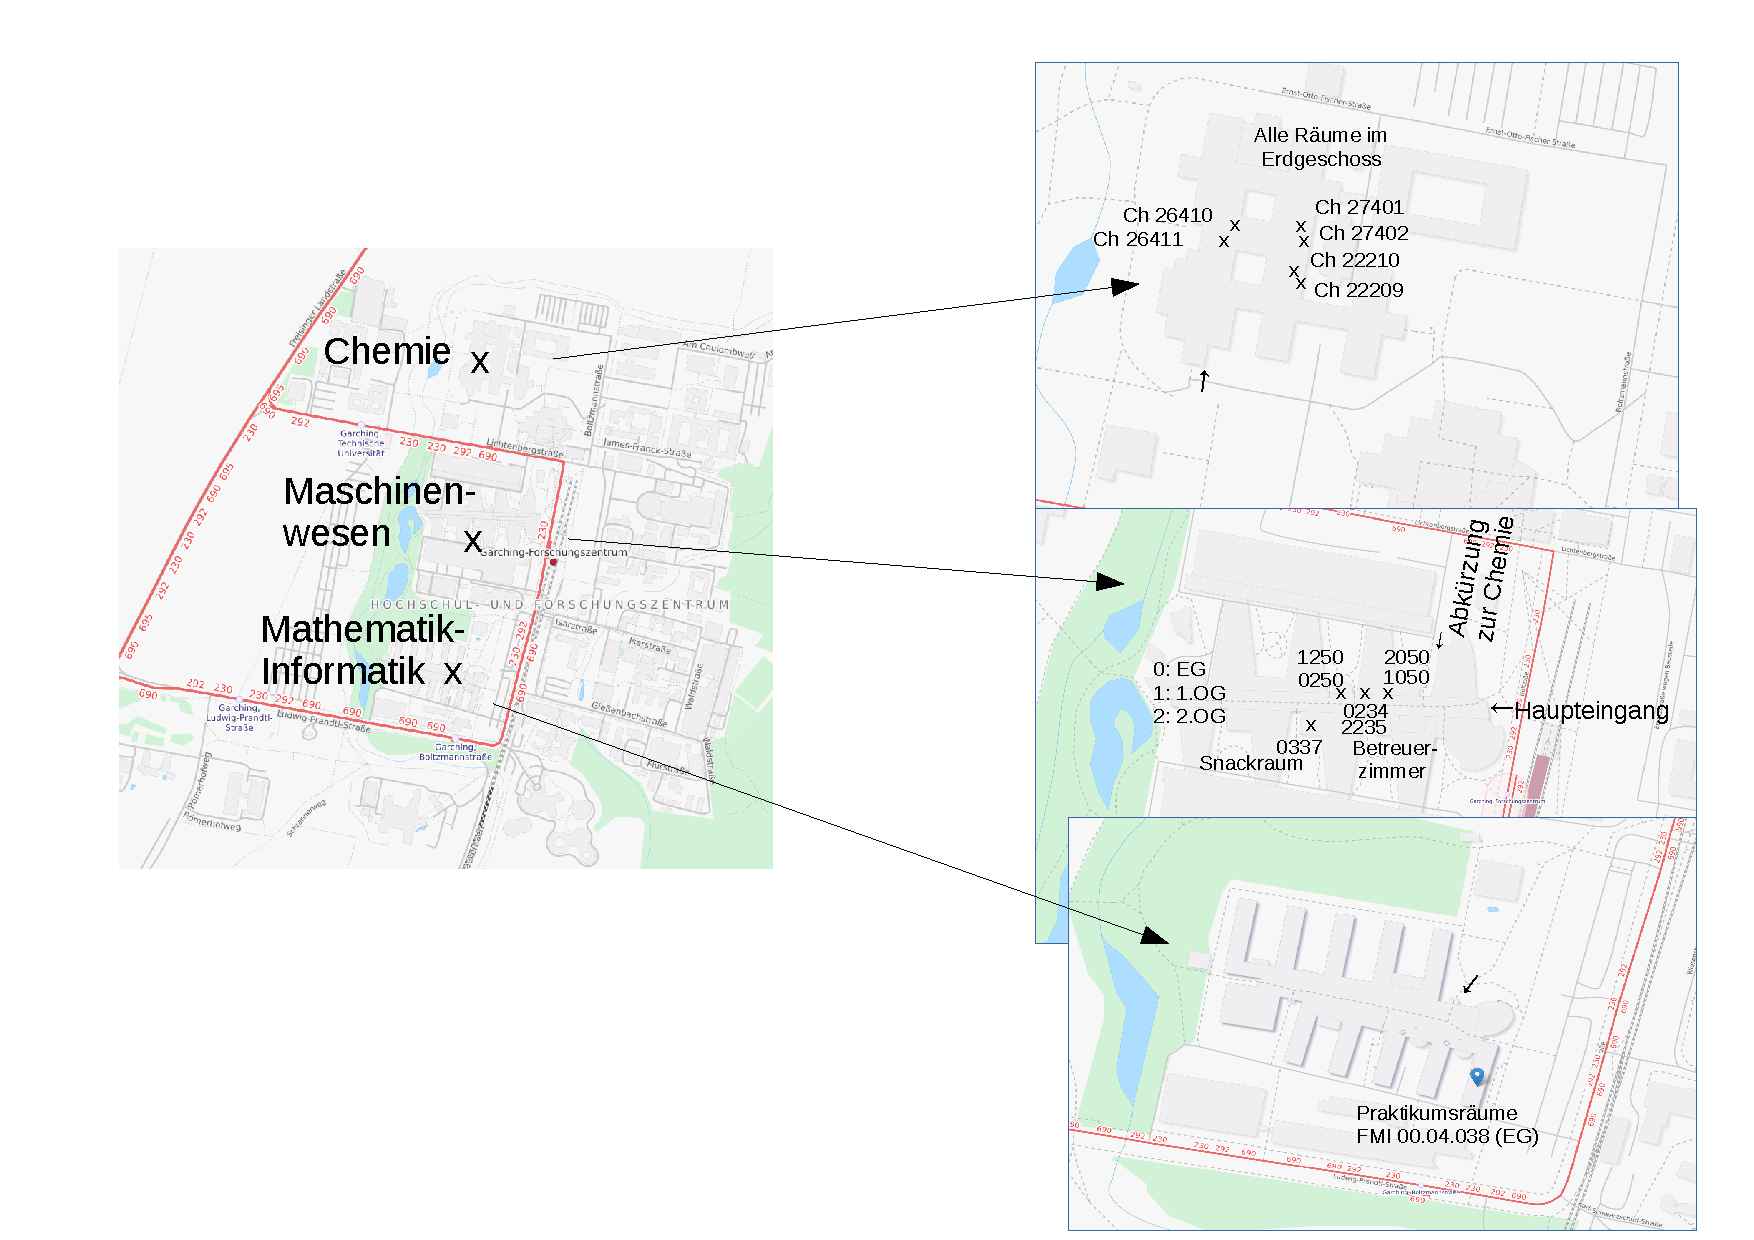
\includegraphics[scale=0.5]{campus_map.pdf}
\end{figure}
\newpage{}\begin{center}{\huge{}\textbf{Stundenplan von Auguste Medert}}\end{center}\textbf{{\large{}Donnerstag}}\nopagebreak \\\begin{tabular} {|p{3cm} p{6cm} p{6cm}| }\hline \textbf{11:30 bis 13:45}&\textbf{Anreise zur TU München}&\textbf{Fakultät Maschinenwesen}\\\hline \textbf{12:00 bis 13:30}&\textbf{Mittagessen}&\textbf{Mensa Garching}\\\hline \textbf{14:00}&\textbf{Begrüßung}&\textbf{CH 26411}\\&Begrüßung, Besprechung des Zeitplans, Ausgabe der individuellen Stundenpläne,...&\\\hline \textbf{14:50 bis 16:20}&\textbf{Quanten- und Atomphysik I}&\textbf{CH 26410}\\&Betreuer: Ismail Achmed-Zade&ca. 28 Teilnehmer\\\hline \textbf{16:40 bis 18:10}&\textbf{Experimentieren und Auswerten}&\textbf{CH 26411}\\&Betreuer: Ann-Kathrin Raab&ca. 15 Teilnehmer\\\hline \textbf{18:30}&\textbf{Fahrt zur Jugendherberge}&\textbf{}\\\hline \textbf{19:00}&\textbf{Abendessen}&\textbf{Jugendherberge}\\\hline \end{tabular}\\\vspace{5.00000mm}~\\\textbf{{\large{}Freitag}}\nopagebreak \\\begin{tabular} {|p{3cm} p{6cm} p{6cm}| }\hline \textbf{06:30 bis 09:00}&\textbf{Frühstück}&\textbf{Jugendherberge}\\\hline \textbf{09:00 bis 13:00}&\textbf{Besichtigung der Forschungsneutronenquelle FRM II}&\textbf{MW 2050}\\&Betreuer: Felix Wechsler&ca. 28 Teilnehmer\\\hline \textbf{13:00 bis 14:00}&\textbf{Mittagessen}&\textbf{Mensa Garching}\\\hline \textbf{14:20 bis 15:50}&\textbf{Gewöhnliche Differentialgleichungen}&\textbf{MW 1250}\\&Betreuer: Sven Jandura&ca. 20 Teilnehmer\\\hline \textbf{16:10 bis 17:40}&\textbf{Spezielle Relativitätstheorie}&\textbf{MW 1250}\\&Betreuer: Johannes Rothe&ca. 19 Teilnehmer\\\hline \textbf{18:00 bis 18:20}&\textbf{Erlebnisbericht IPhO}&\textbf{CH 26411}\\\hline \textbf{18:30}&\textbf{Fahrt zur Jugendherberge}&\textbf{}\\\hline \textbf{19:00}&\textbf{Abendessen}&\textbf{Jugendherberge}\\\hline \end{tabular}\\\vspace{5.00000mm}~\\\textbf{{\large{}Samstag}}\nopagebreak \\\begin{tabular} {|p{3cm} p{6cm} p{6cm}| }\hline \textbf{06:30 bis 08:00}&\textbf{Frühstück}&\textbf{Jugendherberge}\\\hline \textbf{08:00}&\textbf{Fahrt zur TU}&\textbf{}\\\hline \textbf{09:00 bis 10:30}&\textbf{Elektrodynamik 1}&\textbf{MW 1250}\\&Betreuer: Maximilian Keitel&ca. 21 Teilnehmer\\\hline \textbf{10:50 bis 12:20}&\textbf{Elektrodynamik 2}&\textbf{MW 1250}\\&Betreuer: Maximilian Keitel&ca. 21 Teilnehmer\\\hline \textbf{12:40 bis 14:00}&\textbf{Mittagessen}&\textbf{Fakultät Maschinenwesen}\\\hline \textbf{14:20 bis 15:50}&\textbf{Elektrische Schaltungen}&\textbf{CH 26410}\\&Betreuer: Felix Wechsler&ca. 4 Teilnehmer\\\hline \textbf{16:10 bis 17:40}&\textbf{Aufgabenseminar Elektrodynamik}&\textbf{MW 1250}\\&Betreuer: Maximilian Keitel&ca. 8 Teilnehmer\\\hline \textbf{18:00 bis 18:20}&\textbf{Vorstellung GYPT}&\textbf{CH 26411}\\\hline \textbf{18:30}&\textbf{Fahrt zur Jugendherberge}&\textbf{}\\\hline \textbf{19:00}&\textbf{Abendessen}&\textbf{Jugendherberge}\\\hline \end{tabular}\\\vspace{5.00000mm}~\\\textbf{{\large{}Sonntag}}\nopagebreak \\\begin{tabular} {|p{3cm} p{6cm} p{6cm}| }\hline \textbf{06:30 bis 08:00}&\textbf{Frühstück}&\textbf{Jugendherberge}\\\hline \textbf{08:00}&\textbf{Fahrt zur TU}&\textbf{}\\\hline \textbf{09:00 bis 10:30}&\textbf{Gravitationsbeschleunigung}&\textbf{MW 1050}\\&Betreuer: Ann-Kathrin Raab&ca. 8 Teilnehmer\\\hline \textbf{10:50 bis 12:20}&\textbf{Relativistische Teilchenphysik}&\textbf{CH 22210}\\&Betreuer: Lars Dehlwes&ca. 11 Teilnehmer\\\hline \textbf{12:40 bis 13:00}&\textbf{Verabschiedung}&\textbf{CH 26411}\\\hline \textbf{13:00}&\textbf{Individuelle Abreise}&\textbf{}\\\hline \textbf{13:00 bis 14:00}&\textbf{Mittagessen}&\textbf{}\\\hline \end{tabular}\\\vspace{5.00000mm}~\\
Notfallnummern: \\
Sven Jandura: xxxx xxxxxxxxx \\
Johannes Rothe: xxxx xxxxxxxxx \\

\large Hast du Lust, die Andern vom Seminar wiederzusehen?\\
\normalsize Dann komm doch einfach zum \textbf{Vereinstreffen}. Dazu musst du kein Vereinsmitglied sein. Neben interesannten Vorträgen und Exkursionen sind jede Menge Spiel und Spaß geplant. Schau in einem Monat einfach noch mal auf der Website vorbei. Wir freuen uns, wenn du dabei bist.

\begin{figure}[!h]
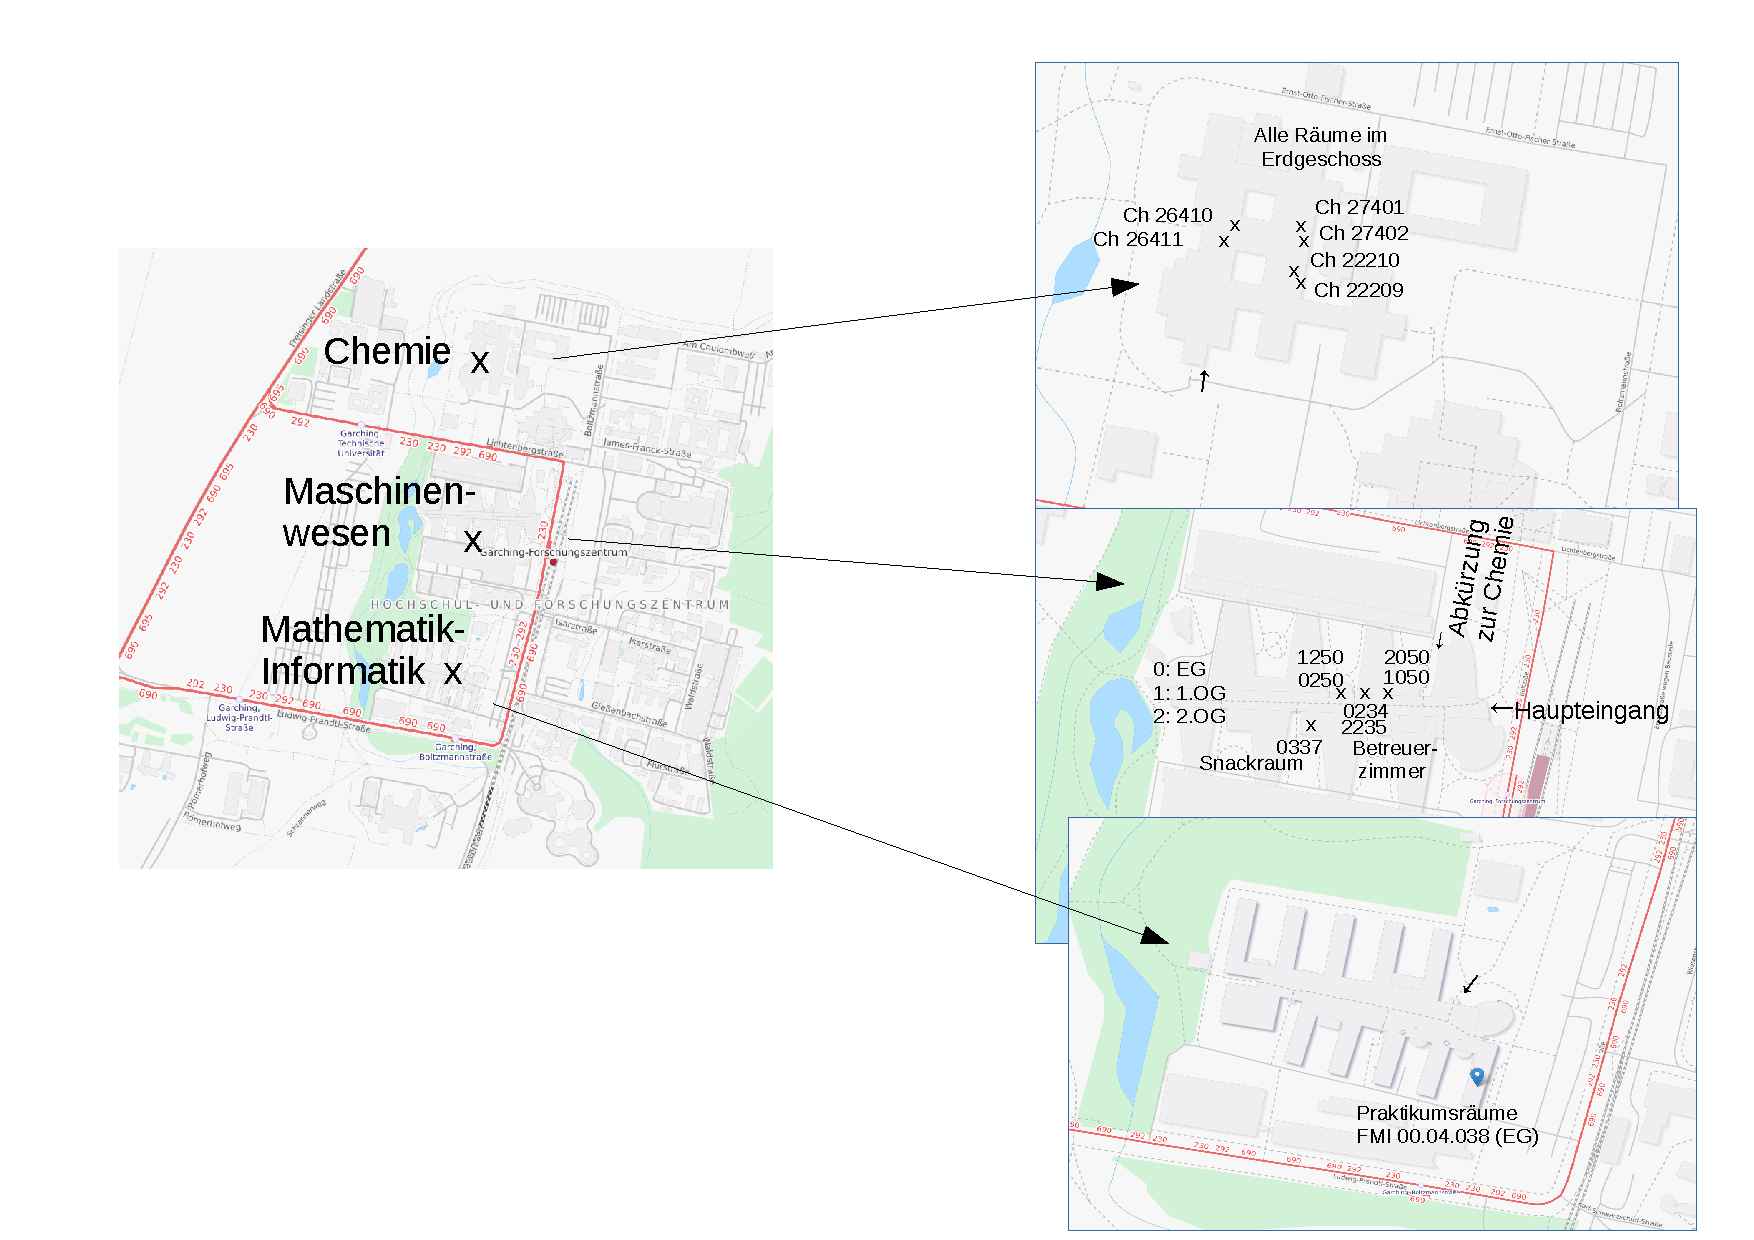
\includegraphics[scale=0.5]{campus_map.pdf}
\end{figure}
\newpage{}\begin{center}{\huge{}\textbf{Stundenplan von Avital Sievers}}\end{center}\textbf{{\large{}Donnerstag}}\nopagebreak \\\begin{tabular} {|p{3cm} p{6cm} p{6cm}| }\hline \textbf{11:30 bis 13:45}&\textbf{Anreise zur TU München}&\textbf{Fakultät Maschinenwesen}\\\hline \textbf{12:00 bis 13:30}&\textbf{Mittagessen}&\textbf{Mensa Garching}\\\hline \textbf{14:00}&\textbf{Begrüßung}&\textbf{CH 26411}\\&Begrüßung, Besprechung des Zeitplans, Ausgabe der individuellen Stundenpläne,...&\\\hline \textbf{14:50 bis 16:20}&\textbf{Quanten- und Atomphysik I}&\textbf{CH 26410}\\&Betreuer: Ismail Achmed-Zade&ca. 28 Teilnehmer\\\hline \textbf{16:40 bis 18:10}&\textbf{Himmelsmechanik}&\textbf{MW 2050}\\&Betreuer: Lars Dehlwes&ca. 19 Teilnehmer\\\hline \textbf{18:30}&\textbf{Fahrt zur Jugendherberge}&\textbf{}\\\hline \textbf{19:00}&\textbf{Abendessen}&\textbf{Jugendherberge}\\\hline \end{tabular}\\\vspace{5.00000mm}~\\\textbf{{\large{}Freitag}}\nopagebreak \\\begin{tabular} {|p{3cm} p{6cm} p{6cm}| }\hline \textbf{06:30 bis 09:00}&\textbf{Frühstück}&\textbf{Jugendherberge}\\\hline \textbf{09:00 bis 13:00}&frei&\\\hline \textbf{13:00 bis 14:00}&\textbf{Mittagessen}&\textbf{Mensa Garching}\\\hline \textbf{14:20 bis 15:50}&\textbf{Gewöhnliche Differentialgleichungen}&\textbf{MW 1250}\\&Betreuer: Sven Jandura&ca. 20 Teilnehmer\\\hline \textbf{16:10 bis 17:40}&\textbf{Näherungsmethoden}&\textbf{CH 26410}\\&Betreuer: Vincent Grande&ca. 11 Teilnehmer\\\hline \textbf{18:00 bis 18:20}&\textbf{Erlebnisbericht IPhO}&\textbf{CH 26411}\\\hline \textbf{18:30}&\textbf{Fahrt zur Jugendherberge}&\textbf{}\\\hline \textbf{19:00}&\textbf{Abendessen}&\textbf{Jugendherberge}\\\hline \end{tabular}\\\vspace{5.00000mm}~\\\textbf{{\large{}Samstag}}\nopagebreak \\\begin{tabular} {|p{3cm} p{6cm} p{6cm}| }\hline \textbf{06:30 bis 08:00}&\textbf{Frühstück}&\textbf{Jugendherberge}\\\hline \textbf{08:00}&\textbf{Fahrt zur TU}&\textbf{}\\\hline \textbf{09:00 bis 10:30}&\textbf{Experimentieren und Auswerten}&\textbf{CH 26411}\\&Betreuer: Ann-Kathrin Raab&ca. 18 Teilnehmer\\\hline \textbf{10:50 bis 12:20}&\textbf{Spezielle Relativitätstheorie}&\textbf{MW 0250}\\&Betreuer: Johannes Rothe&ca. 12 Teilnehmer\\\hline \textbf{12:40 bis 14:00}&\textbf{Mittagessen}&\textbf{Fakultät Maschinenwesen}\\\hline \textbf{14:20 bis 15:50}&\textbf{Relativistische Teilchenphysik}&\textbf{CH 22210}\\&Betreuer: Lars Dehlwes&ca. 23 Teilnehmer\\\hline \textbf{16:10 bis 17:40}&\textbf{Komplexe Wechselstromrechnung}&\textbf{MW 0250}\\&Betreuer: Vincent Grande&ca. 13 Teilnehmer\\\hline \textbf{18:00 bis 18:20}&\textbf{Vorstellung GYPT}&\textbf{CH 26411}\\\hline \textbf{18:30}&\textbf{Fahrt zur Jugendherberge}&\textbf{}\\\hline \textbf{19:00}&\textbf{Abendessen}&\textbf{Jugendherberge}\\\hline \end{tabular}\\\vspace{5.00000mm}~\\\textbf{{\large{}Sonntag}}\nopagebreak \\\begin{tabular} {|p{3cm} p{6cm} p{6cm}| }\hline \textbf{06:30 bis 08:00}&\textbf{Frühstück}&\textbf{Jugendherberge}\\\hline \textbf{08:00}&\textbf{Fahrt zur TU}&\textbf{}\\\hline \textbf{09:00 bis 10:30}&\textbf{Theoretische Mechanik}&\textbf{CH 22210}\\&Betreuer: Eugen Dizer&ca. 13 Teilnehmer\\\hline \textbf{10:50 bis 12:20}&\textbf{Aufgabenseminar Quanten- und Atomphysik und Struktur der Materie}&\textbf{MW 1250}\\&Betreuer: Vitaly Andreev&ca. 24 Teilnehmer\\\hline \textbf{12:40 bis 13:00}&\textbf{Verabschiedung}&\textbf{CH 26411}\\\hline \textbf{13:00}&\textbf{Individuelle Abreise}&\textbf{}\\\hline \textbf{13:00 bis 14:00}&\textbf{Mittagessen}&\textbf{}\\\hline \end{tabular}\\\vspace{5.00000mm}~\\
Notfallnummern: \\
Sven Jandura: xxxx xxxxxxxxx \\
Johannes Rothe: xxxx xxxxxxxxx \\

\large Hast du Lust, die Andern vom Seminar wiederzusehen?\\
\normalsize Dann komm doch einfach zum \textbf{Vereinstreffen}. Dazu musst du kein Vereinsmitglied sein. Neben interesannten Vorträgen und Exkursionen sind jede Menge Spiel und Spaß geplant. Schau in einem Monat einfach noch mal auf der Website vorbei. Wir freuen uns, wenn du dabei bist.

\begin{figure}[!h]
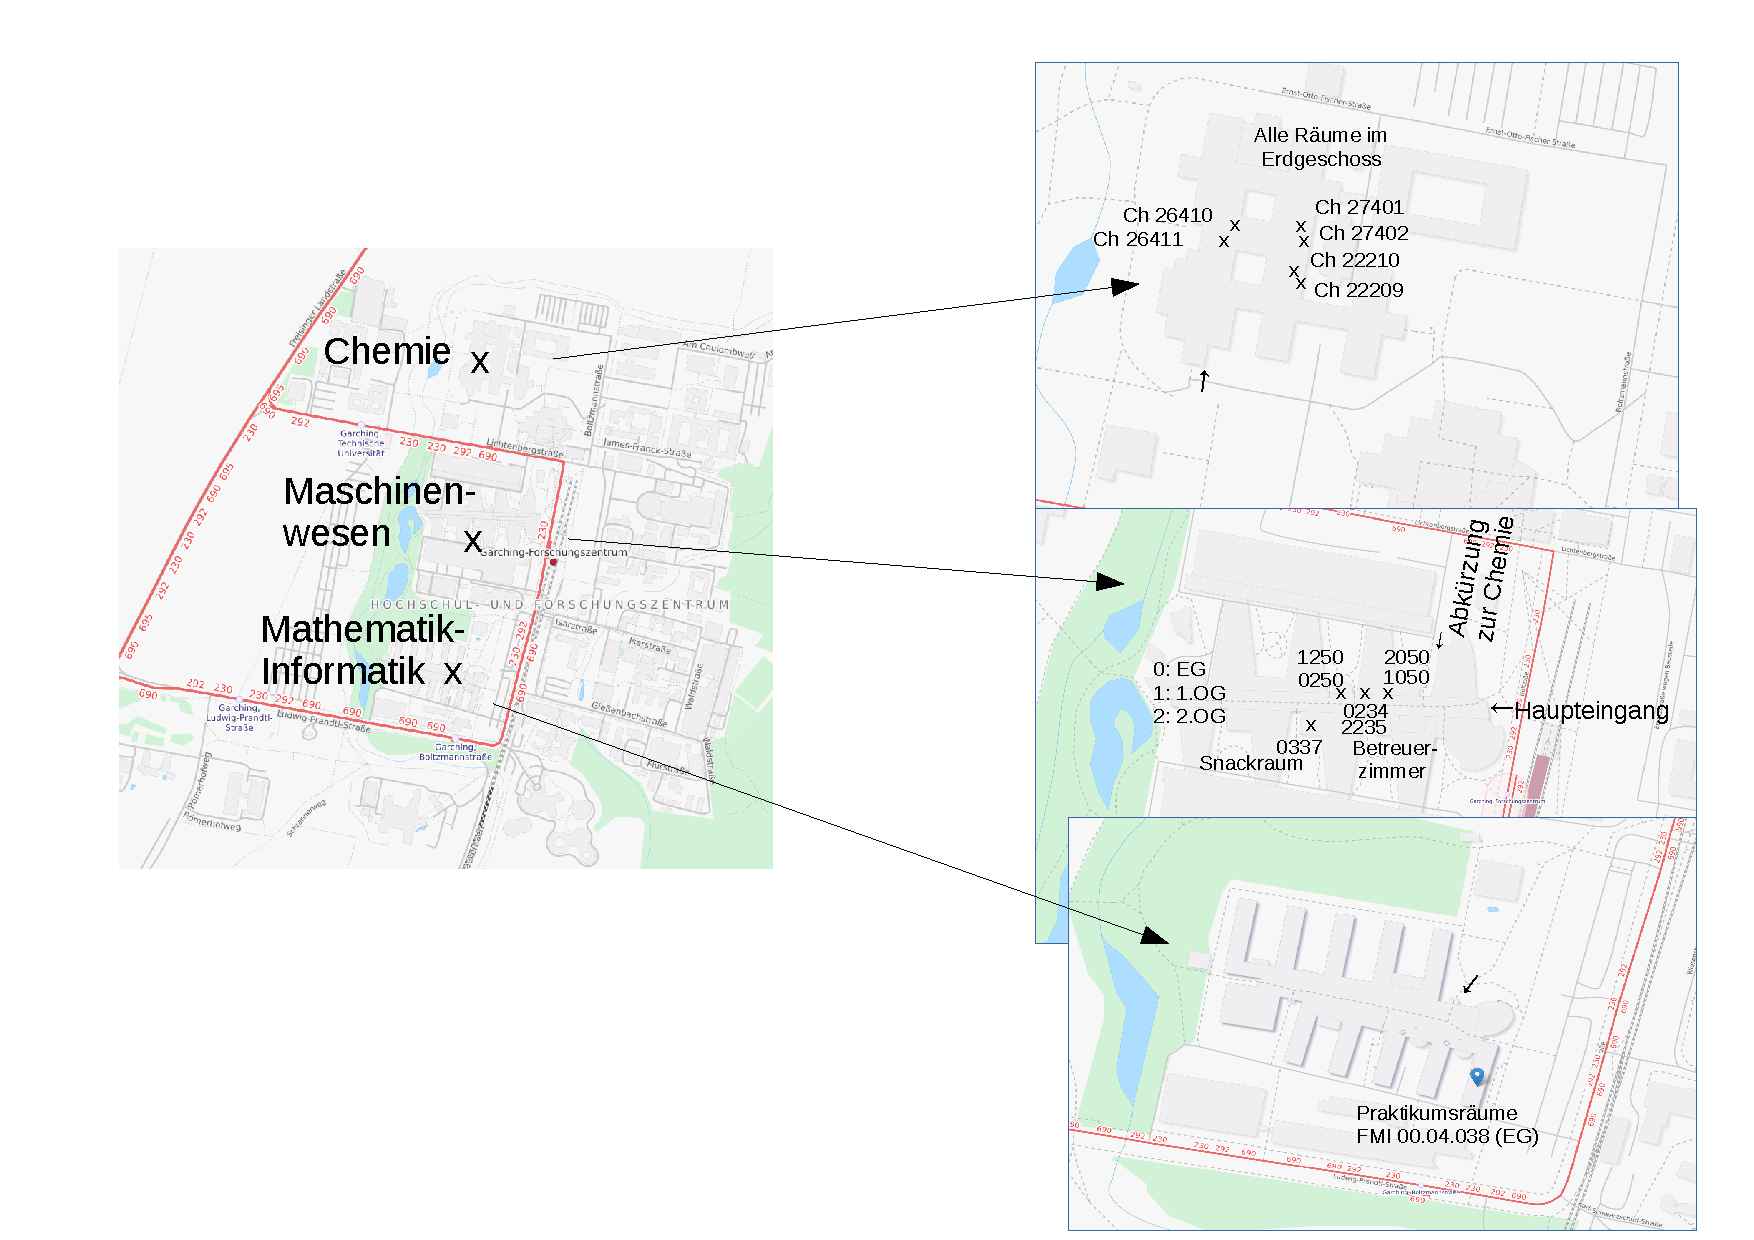
\includegraphics[scale=0.5]{campus_map.pdf}
\end{figure}
\newpage{}\begin{center}{\huge{}\textbf{Stundenplan von Bastian Hesbacher}}\end{center}\textbf{{\large{}Donnerstag}}\nopagebreak \\\begin{tabular} {|p{3cm} p{6cm} p{6cm}| }\hline \textbf{11:30 bis 13:45}&\textbf{Anreise zur TU München}&\textbf{Fakultät Maschinenwesen}\\\hline \textbf{12:00 bis 13:30}&\textbf{Mittagessen}&\textbf{Mensa Garching}\\\hline \textbf{14:00}&\textbf{Begrüßung}&\textbf{CH 26411}\\&Begrüßung, Besprechung des Zeitplans, Ausgabe der individuellen Stundenpläne,...&\\\hline \textbf{14:50 bis 16:20}&\textbf{Thermodynamik 1}&\textbf{MW 1250}\\&Betreuer: Maximilian Marienhagen&ca. 12 Teilnehmer\\\hline \textbf{16:40 bis 18:10}&\textbf{Himmelsmechanik}&\textbf{MW 2050}\\&Betreuer: Lars Dehlwes&ca. 19 Teilnehmer\\\hline \textbf{18:30}&\textbf{Fahrt zur Jugendherberge}&\textbf{}\\\hline \textbf{19:00}&\textbf{Abendessen}&\textbf{Jugendherberge}\\\hline \end{tabular}\\\vspace{5.00000mm}~\\\textbf{{\large{}Freitag}}\nopagebreak \\\begin{tabular} {|p{3cm} p{6cm} p{6cm}| }\hline \textbf{06:30 bis 09:00}&\textbf{Frühstück}&\textbf{Jugendherberge}\\\hline \textbf{09:00 bis 13:00}&\textbf{Besichtigung der Forschungsneutronenquelle FRM II}&\textbf{MW 2050}\\&Betreuer: Felix Wechsler&ca. 28 Teilnehmer\\\hline \textbf{13:00 bis 14:00}&\textbf{Mittagessen}&\textbf{Mensa Garching}\\\hline \textbf{14:20 bis 15:50}&\textbf{Kernphysik}&\textbf{MW 0250}\\&Betreuer: Johannes Rothe&ca. 18 Teilnehmer\\\hline \textbf{16:10 bis 17:40}&\textbf{Einführung ins Integrieren}&\textbf{MW 2050}\\&Betreuer: Felix Wechsler&ca. 14 Teilnehmer\\\hline \textbf{18:00 bis 18:20}&\textbf{Erlebnisbericht IPhO}&\textbf{CH 26411}\\\hline \textbf{18:30}&\textbf{Fahrt zur Jugendherberge}&\textbf{}\\\hline \textbf{19:00}&\textbf{Abendessen}&\textbf{Jugendherberge}\\\hline \end{tabular}\\\vspace{5.00000mm}~\\\textbf{{\large{}Samstag}}\nopagebreak \\\begin{tabular} {|p{3cm} p{6cm} p{6cm}| }\hline \textbf{06:30 bis 08:00}&\textbf{Frühstück}&\textbf{Jugendherberge}\\\hline \textbf{08:00}&\textbf{Fahrt zur TU}&\textbf{}\\\hline \textbf{09:00 bis 10:30}&\textbf{Experimentieren und Auswerten}&\textbf{CH 26411}\\&Betreuer: Ann-Kathrin Raab&ca. 18 Teilnehmer\\\hline \textbf{10:50 bis 12:20}&\textbf{Quanten- und Atomphysik I}&\textbf{MW 2050}\\&Betreuer: Vitaly Andreev&ca. 13 Teilnehmer\\\hline \textbf{12:40 bis 14:00}&\textbf{Mittagessen}&\textbf{Fakultät Maschinenwesen}\\\hline \textbf{14:20 bis 15:50}&\textbf{Bestimmung des Brechungskoeffizienten von Plexiglas}&\textbf{MW 0234}\\&Betreuer: Lilith Diringer&ca. 8 Teilnehmer\\\hline \textbf{16:10 bis 17:40}&\textbf{Quanten- und Atomphysik II}&\textbf{CH 22209}\\&Betreuer: Vitaly Andreev&ca. 28 Teilnehmer\\\hline \textbf{18:00 bis 18:20}&\textbf{Vorstellung GYPT}&\textbf{CH 26411}\\\hline \textbf{18:30}&\textbf{Fahrt zur Jugendherberge}&\textbf{}\\\hline \textbf{19:00}&\textbf{Abendessen}&\textbf{Jugendherberge}\\\hline \end{tabular}\\\vspace{5.00000mm}~\\\textbf{{\large{}Sonntag}}\nopagebreak \\\begin{tabular} {|p{3cm} p{6cm} p{6cm}| }\hline \textbf{06:30 bis 08:00}&\textbf{Frühstück}&\textbf{Jugendherberge}\\\hline \textbf{08:00}&\textbf{Fahrt zur TU}&\textbf{}\\\hline \textbf{09:00 bis 10:30}&\textbf{Elektronik}&\textbf{CH 26410}\\&Betreuer: Martin Großhauser&ca. 10 Teilnehmer\\\hline \textbf{10:50 bis 12:20}&\textbf{Aufgabenseminar Quanten- und Atomphysik und Struktur der Materie}&\textbf{MW 1250}\\&Betreuer: Vitaly Andreev&ca. 24 Teilnehmer\\\hline \textbf{12:40 bis 13:00}&\textbf{Verabschiedung}&\textbf{CH 26411}\\\hline \textbf{13:00}&\textbf{Individuelle Abreise}&\textbf{}\\\hline \textbf{13:00 bis 14:00}&\textbf{Mittagessen}&\textbf{}\\\hline \end{tabular}\\\vspace{5.00000mm}~\\
Notfallnummern: \\
Sven Jandura: xxxx xxxxxxxxx \\
Johannes Rothe: xxxx xxxxxxxxx \\

\large Hast du Lust, die Andern vom Seminar wiederzusehen?\\
\normalsize Dann komm doch einfach zum \textbf{Vereinstreffen}. Dazu musst du kein Vereinsmitglied sein. Neben interesannten Vorträgen und Exkursionen sind jede Menge Spiel und Spaß geplant. Schau in einem Monat einfach noch mal auf der Website vorbei. Wir freuen uns, wenn du dabei bist.

\begin{figure}[!h]
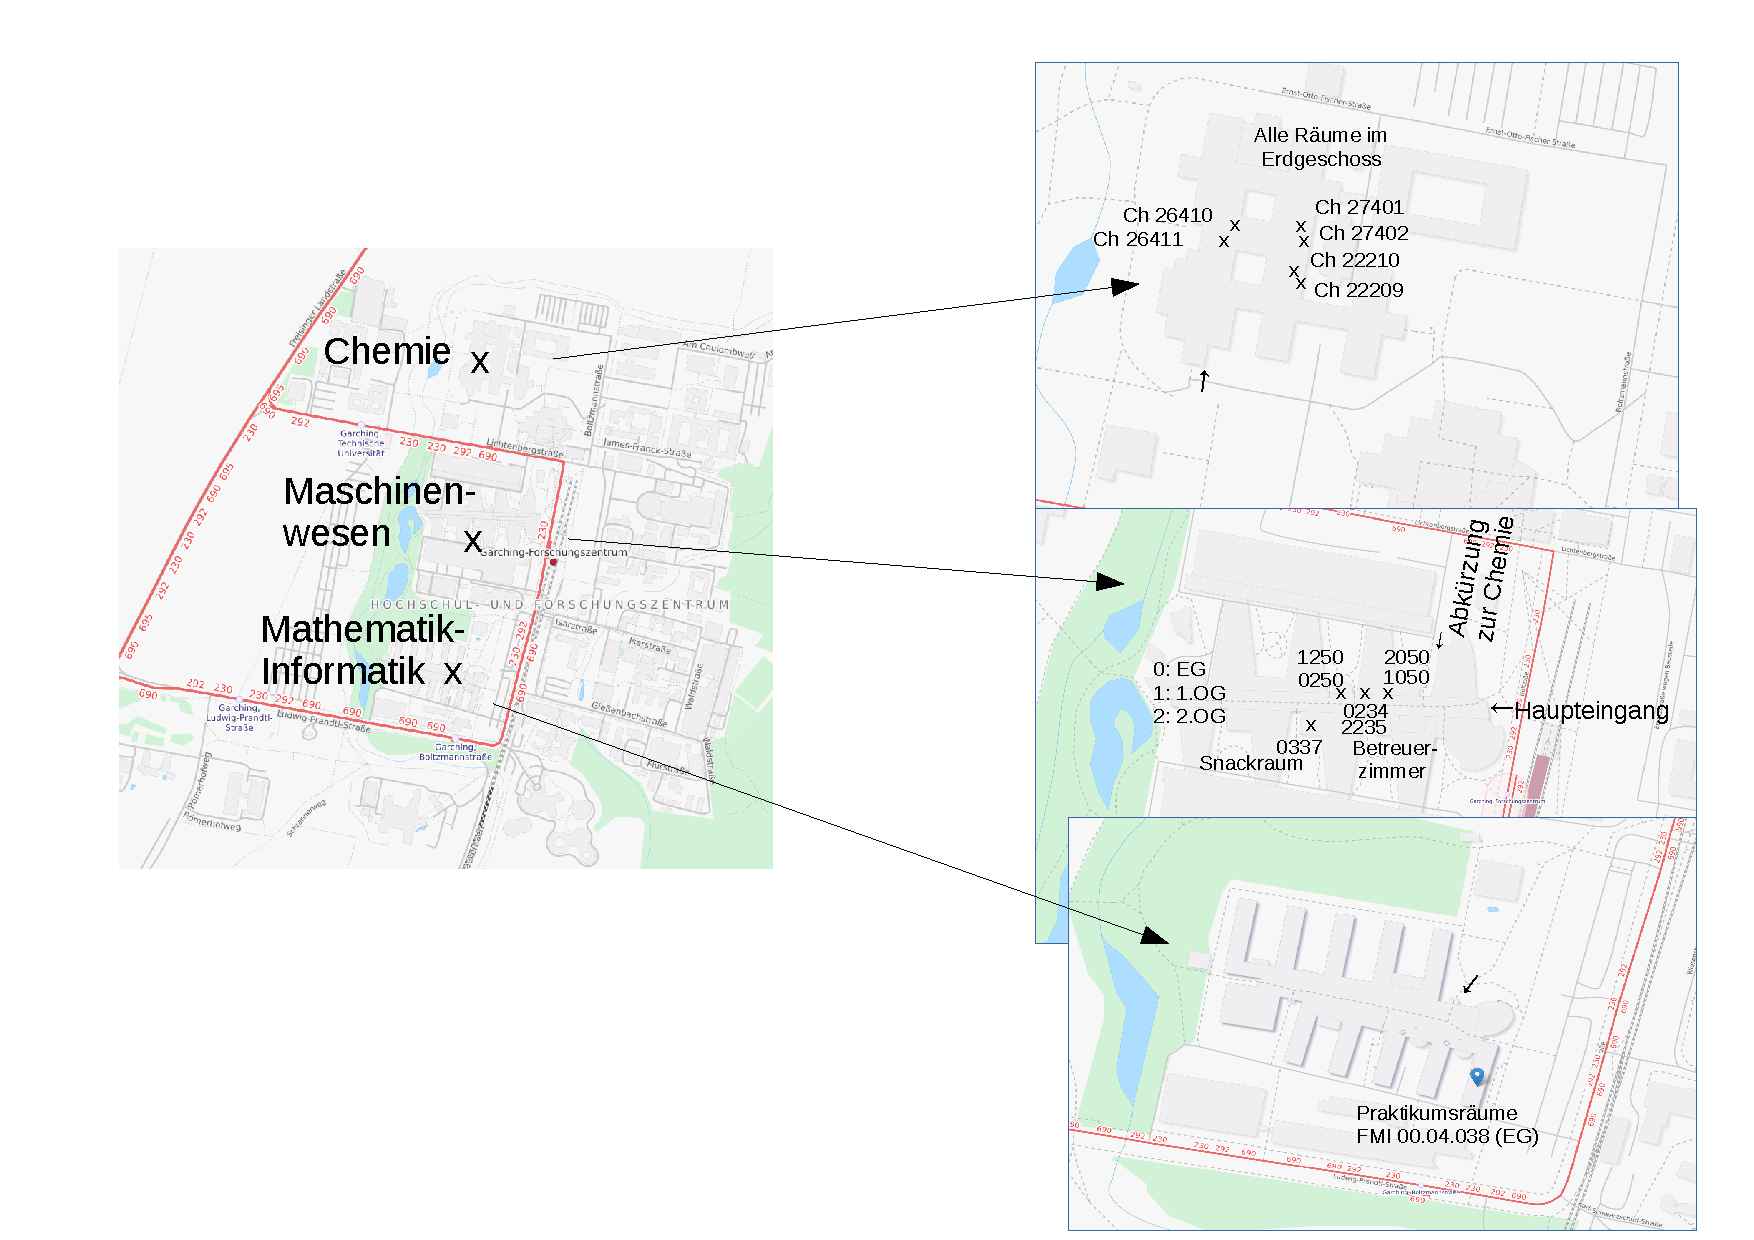
\includegraphics[scale=0.5]{campus_map.pdf}
\end{figure}
\newpage{}\begin{center}{\huge{}\textbf{Stundenplan von Benedikt Wahl}}\end{center}\textbf{{\large{}Donnerstag}}\nopagebreak \\\begin{tabular} {|p{3cm} p{6cm} p{6cm}| }\hline \textbf{11:30 bis 13:45}&\textbf{Anreise zur TU München}&\textbf{Fakultät Maschinenwesen}\\\hline \textbf{12:00 bis 13:30}&\textbf{Mittagessen}&\textbf{Mensa Garching}\\\hline \textbf{14:00}&\textbf{Begrüßung}&\textbf{CH 26411}\\&Begrüßung, Besprechung des Zeitplans, Ausgabe der individuellen Stundenpläne,...&\\\hline \textbf{14:50 bis 16:20}&\textbf{Elektrische Schaltungen}&\textbf{MW 0250}\\&Betreuer: Christopher Pfeiffer&ca. 16 Teilnehmer\\\hline \textbf{16:40 bis 18:10}&\textbf{Experimentieren und Auswerten}&\textbf{CH 26411}\\&Betreuer: Ann-Kathrin Raab&ca. 15 Teilnehmer\\\hline \textbf{18:30}&\textbf{Fahrt zur Jugendherberge}&\textbf{}\\\hline \textbf{19:00}&\textbf{Abendessen}&\textbf{Jugendherberge}\\\hline \end{tabular}\\\vspace{5.00000mm}~\\\textbf{{\large{}Freitag}}\nopagebreak \\\begin{tabular} {|p{3cm} p{6cm} p{6cm}| }\hline \textbf{06:30 bis 09:00}&\textbf{Frühstück}&\textbf{Jugendherberge}\\\hline \textbf{09:00 bis 13:00}&frei&\\\hline \textbf{13:00 bis 14:00}&\textbf{Mittagessen}&\textbf{Mensa Garching}\\\hline \textbf{14:20 bis 15:50}&\textbf{Gewöhnliche Differentialgleichungen}&\textbf{MW 1250}\\&Betreuer: Sven Jandura&ca. 20 Teilnehmer\\\hline \textbf{16:10 bis 17:40}&\textbf{Experiment Brückenschaltung}&\textbf{Praktikum Brückenschaltung}\\&Betreuer: Martin Großhauser&ca. 6 Teilnehmer\\\hline \textbf{18:00 bis 18:20}&\textbf{Erlebnisbericht IPhO}&\textbf{CH 26411}\\\hline \textbf{18:30}&\textbf{Fahrt zur Jugendherberge}&\textbf{}\\\hline \textbf{19:00}&\textbf{Abendessen}&\textbf{Jugendherberge}\\\hline \end{tabular}\\\vspace{5.00000mm}~\\\textbf{{\large{}Samstag}}\nopagebreak \\\begin{tabular} {|p{3cm} p{6cm} p{6cm}| }\hline \textbf{06:30 bis 08:00}&\textbf{Frühstück}&\textbf{Jugendherberge}\\\hline \textbf{08:00}&\textbf{Fahrt zur TU}&\textbf{}\\\hline \textbf{09:00 bis 10:30}&\textbf{Experiment Brennstoffzelle}&\textbf{Praktikum Brennstoffzelle}\\&Betreuer: Aaron Wild&ca. 6 Teilnehmer\\\hline \textbf{10:50 bis 12:20}&\textbf{Experiment Pohlsches Rad}&\textbf{Praktikum Pohlsches Rad}\\&Betreuer: Eugen Dizer&ca. 4 Teilnehmer\\\hline \textbf{12:40 bis 14:00}&\textbf{Mittagessen}&\textbf{Fakultät Maschinenwesen}\\\hline \textbf{14:20 bis 15:50}&\textbf{Quanten- und Atomphysik I}&\textbf{CH 22209}\\&Betreuer: Vitaly Andreev&ca. 22 Teilnehmer\\\hline \textbf{16:10 bis 17:40}&\textbf{Komplexe Wechselstromrechnung}&\textbf{MW 0250}\\&Betreuer: Vincent Grande&ca. 13 Teilnehmer\\\hline \textbf{18:00 bis 18:20}&\textbf{Vorstellung GYPT}&\textbf{CH 26411}\\\hline \textbf{18:30}&\textbf{Fahrt zur Jugendherberge}&\textbf{}\\\hline \textbf{19:00}&\textbf{Abendessen}&\textbf{Jugendherberge}\\\hline \end{tabular}\\\vspace{5.00000mm}~\\\textbf{{\large{}Sonntag}}\nopagebreak \\\begin{tabular} {|p{3cm} p{6cm} p{6cm}| }\hline \textbf{06:30 bis 08:00}&\textbf{Frühstück}&\textbf{Jugendherberge}\\\hline \textbf{08:00}&\textbf{Fahrt zur TU}&\textbf{}\\\hline \textbf{09:00 bis 10:30}&\textbf{Aufgabenseminar Elektrodynamik}&\textbf{MW 0234}\\&Betreuer: Maximilian Keitel&ca. 4 Teilnehmer\\\hline \textbf{10:50 bis 12:20}&\textbf{Elektrische Blackboxen}&\textbf{Praktikum Blackboxen}\\&Betreuer: Eugen Dizer&ca. 6 Teilnehmer\\\hline \textbf{12:40 bis 13:00}&\textbf{Verabschiedung}&\textbf{CH 26411}\\\hline \textbf{13:00}&\textbf{Individuelle Abreise}&\textbf{}\\\hline \textbf{13:00 bis 14:00}&\textbf{Mittagessen}&\textbf{}\\\hline \end{tabular}\\\vspace{5.00000mm}~\\
Notfallnummern: \\
Sven Jandura: xxxx xxxxxxxxx \\
Johannes Rothe: xxxx xxxxxxxxx \\

\large Hast du Lust, die Andern vom Seminar wiederzusehen?\\
\normalsize Dann komm doch einfach zum \textbf{Vereinstreffen}. Dazu musst du kein Vereinsmitglied sein. Neben interesannten Vorträgen und Exkursionen sind jede Menge Spiel und Spaß geplant. Schau in einem Monat einfach noch mal auf der Website vorbei. Wir freuen uns, wenn du dabei bist.

\begin{figure}[!h]
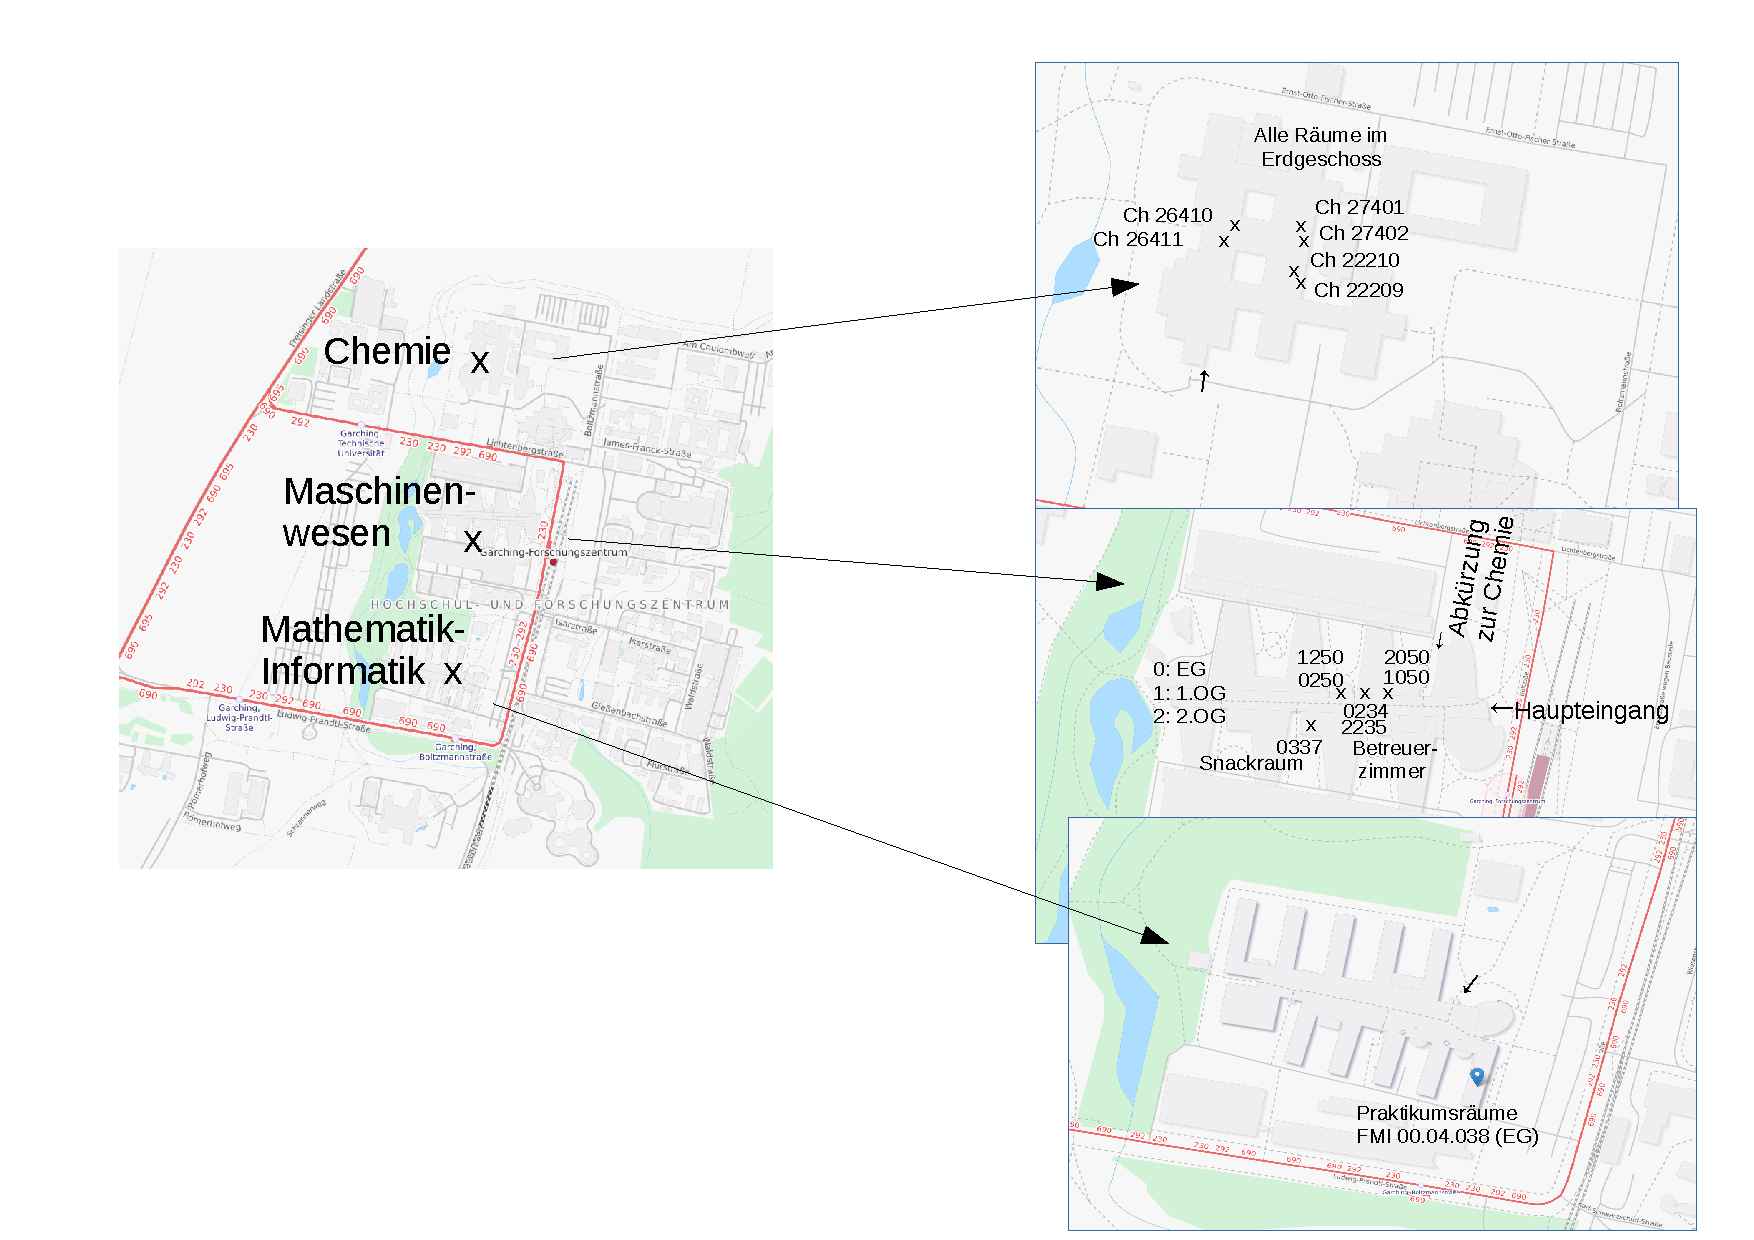
\includegraphics[scale=0.5]{campus_map.pdf}
\end{figure}
\newpage{}\begin{center}{\huge{}\textbf{Stundenplan von Brendan Berg}}\end{center}\textbf{{\large{}Donnerstag}}\nopagebreak \\\begin{tabular} {|p{3cm} p{6cm} p{6cm}| }\hline \textbf{11:30 bis 13:45}&\textbf{Anreise zur TU München}&\textbf{Fakultät Maschinenwesen}\\\hline \textbf{12:00 bis 13:30}&\textbf{Mittagessen}&\textbf{Mensa Garching}\\\hline \textbf{14:00}&\textbf{Begrüßung}&\textbf{CH 26411}\\&Begrüßung, Besprechung des Zeitplans, Ausgabe der individuellen Stundenpläne,...&\\\hline \textbf{14:50 bis 16:20}&\textbf{Quanten- und Atomphysik I}&\textbf{CH 26410}\\&Betreuer: Ismail Achmed-Zade&ca. 28 Teilnehmer\\\hline \textbf{16:40 bis 18:10}&\textbf{Einführung ins Integrieren}&\textbf{MW 1050}\\&Betreuer: Johannes Rothe&ca. 14 Teilnehmer\\\hline \textbf{18:30}&\textbf{Fahrt zur Jugendherberge}&\textbf{}\\\hline \textbf{19:00}&\textbf{Abendessen}&\textbf{Jugendherberge}\\\hline \end{tabular}\\\vspace{5.00000mm}~\\\textbf{{\large{}Freitag}}\nopagebreak \\\begin{tabular} {|p{3cm} p{6cm} p{6cm}| }\hline \textbf{06:30 bis 09:00}&\textbf{Frühstück}&\textbf{Jugendherberge}\\\hline \textbf{09:00 bis 13:00}&\textbf{Besichtigung der Forschungsneutronenquelle FRM II}&\textbf{MW 2050}\\&Betreuer: Felix Wechsler&ca. 28 Teilnehmer\\\hline \textbf{13:00 bis 14:00}&\textbf{Mittagessen}&\textbf{Mensa Garching}\\\hline \textbf{14:20 bis 15:50}&\textbf{Experiment Magnetismus}&\textbf{Praktikum Magnetismus}\\&Betreuer: Lars Dehlwes&ca. 6 Teilnehmer\\\hline \textbf{16:10 bis 17:40}&\textbf{Harmonische Schwingungen}&\textbf{MW 2050}\\&Betreuer: Ilja Göthel&ca. 3 Teilnehmer\\\hline \textbf{18:00 bis 18:20}&\textbf{Erlebnisbericht IPhO}&\textbf{CH 26411}\\\hline \textbf{18:30}&\textbf{Fahrt zur Jugendherberge}&\textbf{}\\\hline \textbf{19:00}&\textbf{Abendessen}&\textbf{Jugendherberge}\\\hline \end{tabular}\\\vspace{5.00000mm}~\\\textbf{{\large{}Samstag}}\nopagebreak \\\begin{tabular} {|p{3cm} p{6cm} p{6cm}| }\hline \textbf{06:30 bis 08:00}&\textbf{Frühstück}&\textbf{Jugendherberge}\\\hline \textbf{08:00}&\textbf{Fahrt zur TU}&\textbf{}\\\hline \textbf{09:00 bis 10:30}&\textbf{Elektrodynamik 1}&\textbf{MW 1250}\\&Betreuer: Maximilian Keitel&ca. 21 Teilnehmer\\\hline \textbf{10:50 bis 12:20}&\textbf{Spezielle Relativitätstheorie}&\textbf{MW 0250}\\&Betreuer: Johannes Rothe&ca. 12 Teilnehmer\\\hline \textbf{12:40 bis 14:00}&\textbf{Mittagessen}&\textbf{Fakultät Maschinenwesen}\\\hline \textbf{14:20 bis 15:50}&\textbf{Elektrodynamik 2}&\textbf{MW 2050}\\&Betreuer: Maximilian Keitel&ca. 6 Teilnehmer\\\hline \textbf{16:10 bis 17:40}&\textbf{Himmelsmechanik}&\textbf{CH 22210}\\&Betreuer: Lars Dehlwes&ca. 10 Teilnehmer\\\hline \textbf{18:00 bis 18:20}&\textbf{Vorstellung GYPT}&\textbf{CH 26411}\\\hline \textbf{18:30}&\textbf{Fahrt zur Jugendherberge}&\textbf{}\\\hline \textbf{19:00}&\textbf{Abendessen}&\textbf{Jugendherberge}\\\hline \end{tabular}\\\vspace{5.00000mm}~\\\textbf{{\large{}Sonntag}}\nopagebreak \\\begin{tabular} {|p{3cm} p{6cm} p{6cm}| }\hline \textbf{06:30 bis 08:00}&\textbf{Frühstück}&\textbf{Jugendherberge}\\\hline \textbf{08:00}&\textbf{Fahrt zur TU}&\textbf{}\\\hline \textbf{09:00 bis 10:30}&\textbf{Wellenoptik}&\textbf{MW 2050}\\&Betreuer: Christopher Pfeiffer&ca. 14 Teilnehmer\\\hline \textbf{10:50 bis 12:20}&\textbf{Elektrische Blackboxen}&\textbf{Praktikum Blackboxen}\\&Betreuer: Eugen Dizer&ca. 6 Teilnehmer\\\hline \textbf{12:40 bis 13:00}&\textbf{Verabschiedung}&\textbf{CH 26411}\\\hline \textbf{13:00}&\textbf{Individuelle Abreise}&\textbf{}\\\hline \textbf{13:00 bis 14:00}&\textbf{Mittagessen}&\textbf{}\\\hline \end{tabular}\\\vspace{5.00000mm}~\\
Notfallnummern: \\
Sven Jandura: xxxx xxxxxxxxx \\
Johannes Rothe: xxxx xxxxxxxxx \\

\large Hast du Lust, die Andern vom Seminar wiederzusehen?\\
\normalsize Dann komm doch einfach zum \textbf{Vereinstreffen}. Dazu musst du kein Vereinsmitglied sein. Neben interesannten Vorträgen und Exkursionen sind jede Menge Spiel und Spaß geplant. Schau in einem Monat einfach noch mal auf der Website vorbei. Wir freuen uns, wenn du dabei bist.

\begin{figure}[!h]
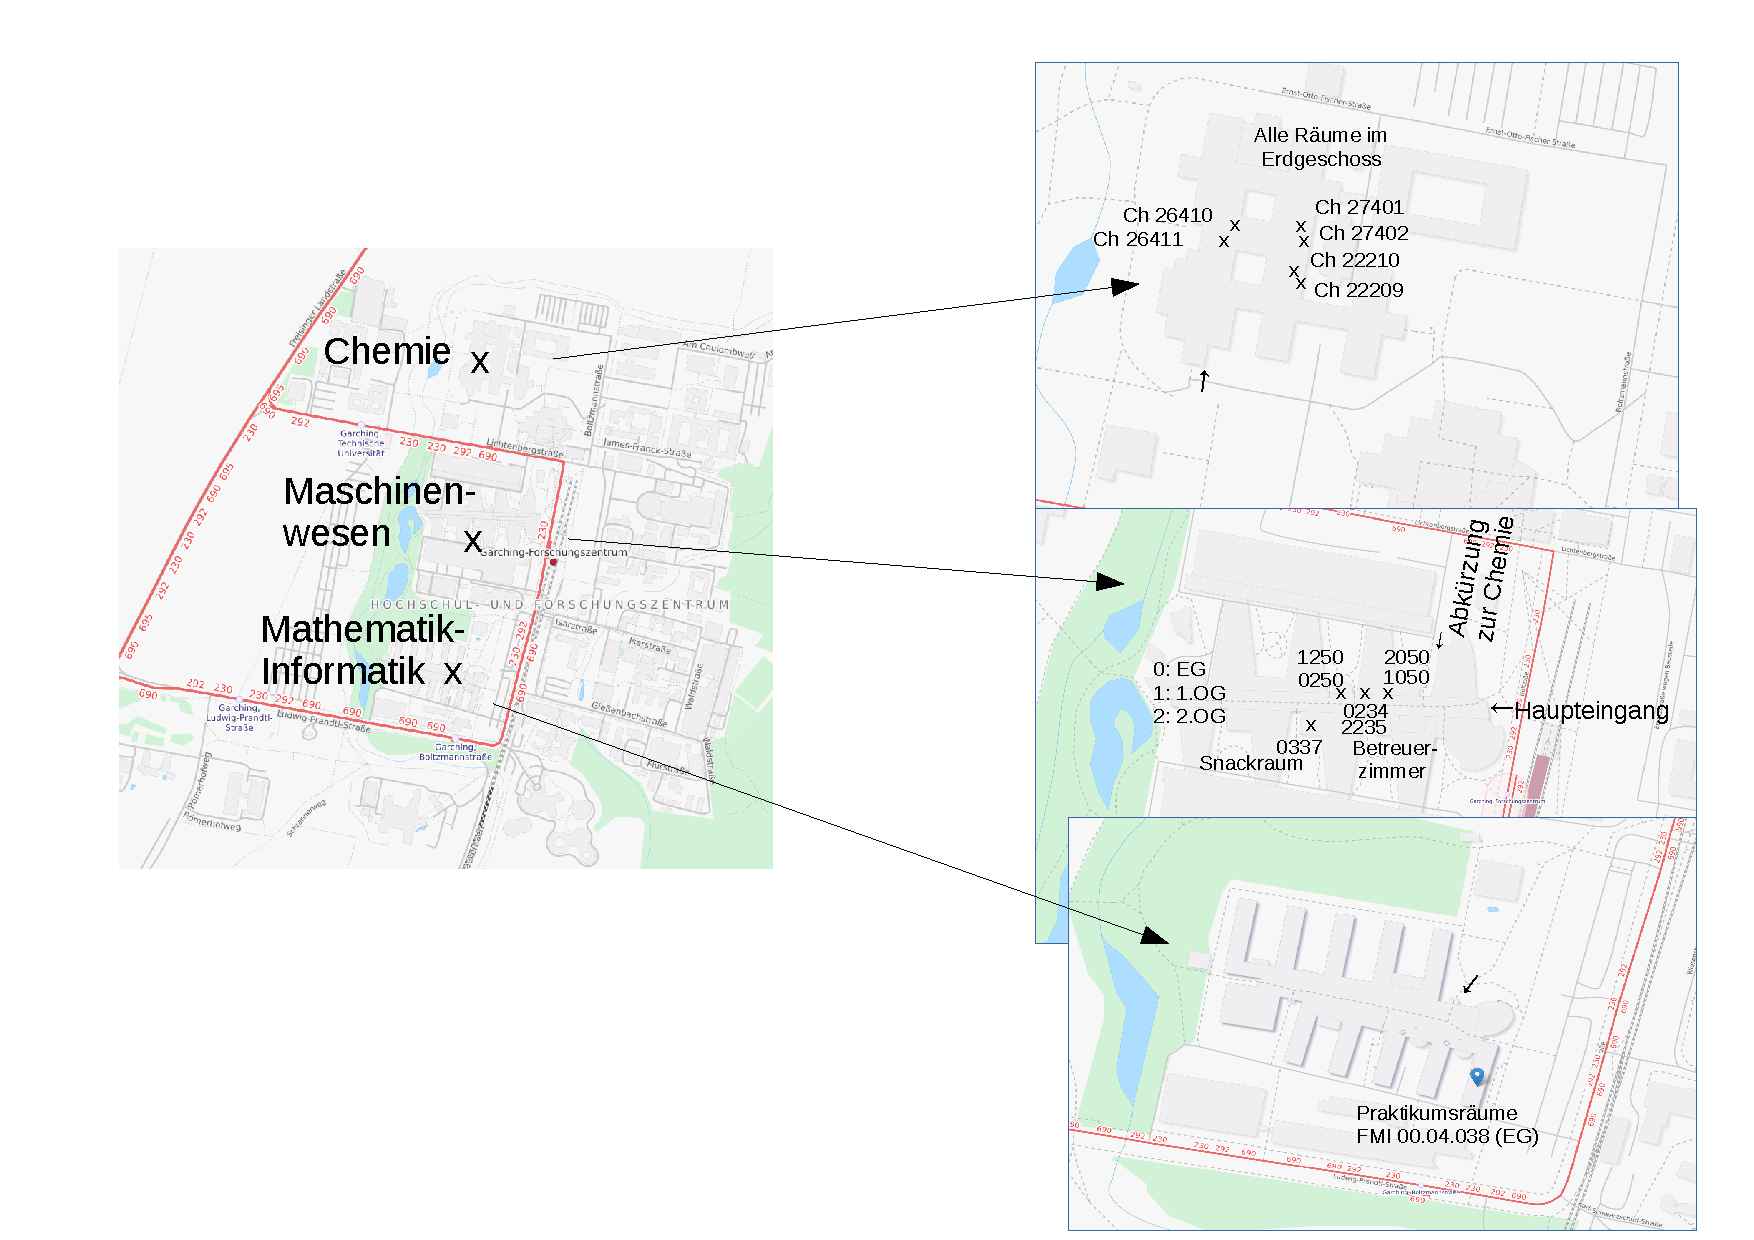
\includegraphics[scale=0.5]{campus_map.pdf}
\end{figure}
\newpage{}\begin{center}{\huge{}\textbf{Stundenplan von Carlotta Gehring}}\end{center}\textbf{{\large{}Donnerstag}}\nopagebreak \\\begin{tabular} {|p{3cm} p{6cm} p{6cm}| }\hline \textbf{11:30 bis 13:45}&\textbf{Anreise zur TU München}&\textbf{Fakultät Maschinenwesen}\\\hline \textbf{12:00 bis 13:30}&\textbf{Mittagessen}&\textbf{Mensa Garching}\\\hline \textbf{14:00}&\textbf{Begrüßung}&\textbf{CH 26411}\\&Begrüßung, Besprechung des Zeitplans, Ausgabe der individuellen Stundenpläne,...&\\\hline \textbf{14:50 bis 16:20}&\textbf{Experimentieren und Auswerten}&\textbf{CH 26411}\\&Betreuer: Ann-Kathrin Raab&ca. 18 Teilnehmer\\\hline \textbf{16:40 bis 18:10}&\textbf{Geometrische Optik}&\textbf{MW 0250}\\&Betreuer: Christopher Pfeiffer&ca. 13 Teilnehmer\\\hline \textbf{18:30}&\textbf{Fahrt zur Jugendherberge}&\textbf{}\\\hline \textbf{19:00}&\textbf{Abendessen}&\textbf{Jugendherberge}\\\hline \end{tabular}\\\vspace{5.00000mm}~\\\textbf{{\large{}Freitag}}\nopagebreak \\\begin{tabular} {|p{3cm} p{6cm} p{6cm}| }\hline \textbf{06:30 bis 09:00}&\textbf{Frühstück}&\textbf{Jugendherberge}\\\hline \textbf{09:00 bis 13:00}&\textbf{Besichtigung der Forschungsneutronenquelle FRM II}&\textbf{MW 2050}\\&Betreuer: Felix Wechsler&ca. 28 Teilnehmer\\\hline \textbf{13:00 bis 14:00}&\textbf{Mittagessen}&\textbf{Mensa Garching}\\\hline \textbf{14:20 bis 15:50}&\textbf{Kernphysik}&\textbf{MW 0250}\\&Betreuer: Johannes Rothe&ca. 18 Teilnehmer\\\hline \textbf{16:10 bis 17:40}&\textbf{Spezielle Relativitätstheorie}&\textbf{MW 1250}\\&Betreuer: Johannes Rothe&ca. 19 Teilnehmer\\\hline \textbf{18:00 bis 18:20}&\textbf{Erlebnisbericht IPhO}&\textbf{CH 26411}\\\hline \textbf{18:30}&\textbf{Fahrt zur Jugendherberge}&\textbf{}\\\hline \textbf{19:00}&\textbf{Abendessen}&\textbf{Jugendherberge}\\\hline \end{tabular}\\\vspace{5.00000mm}~\\\textbf{{\large{}Samstag}}\nopagebreak \\\begin{tabular} {|p{3cm} p{6cm} p{6cm}| }\hline \textbf{06:30 bis 08:00}&\textbf{Frühstück}&\textbf{Jugendherberge}\\\hline \textbf{08:00}&\textbf{Fahrt zur TU}&\textbf{}\\\hline \textbf{09:00 bis 10:30}&\textbf{Aufgabenseminar klassische Mechanik}&\textbf{MW 0234}\\&Betreuer: Maximilian Marienhagen&ca. 5 Teilnehmer\\\hline \textbf{10:50 bis 12:20}&\textbf{Himmelsmechanik}&\textbf{CH 26410}\\&Betreuer: Lars Dehlwes&ca. 6 Teilnehmer\\\hline \textbf{12:40 bis 14:00}&\textbf{Mittagessen}&\textbf{Fakultät Maschinenwesen}\\\hline \textbf{14:20 bis 15:50}&\textbf{Quanten- und Atomphysik I}&\textbf{CH 22209}\\&Betreuer: Vitaly Andreev&ca. 22 Teilnehmer\\\hline \textbf{16:10 bis 17:40}&\textbf{Wellenoptik}&\textbf{CH 26410}\\&Betreuer: Christopher Pfeiffer&ca. 7 Teilnehmer\\\hline \textbf{18:00 bis 18:20}&\textbf{Vorstellung GYPT}&\textbf{CH 26411}\\\hline \textbf{18:30}&\textbf{Fahrt zur Jugendherberge}&\textbf{}\\\hline \textbf{19:00}&\textbf{Abendessen}&\textbf{Jugendherberge}\\\hline \end{tabular}\\\vspace{5.00000mm}~\\\textbf{{\large{}Sonntag}}\nopagebreak \\\begin{tabular} {|p{3cm} p{6cm} p{6cm}| }\hline \textbf{06:30 bis 08:00}&\textbf{Frühstück}&\textbf{Jugendherberge}\\\hline \textbf{08:00}&\textbf{Fahrt zur TU}&\textbf{}\\\hline \textbf{09:00 bis 10:30}&\textbf{Quanten- und Atomphysik II}&\textbf{MW 1250}\\&Betreuer: Vitaly Andreev&ca. 15 Teilnehmer\\\hline \textbf{10:50 bis 12:20}&\textbf{Relativistische Teilchenphysik}&\textbf{CH 22210}\\&Betreuer: Lars Dehlwes&ca. 11 Teilnehmer\\\hline \textbf{12:40 bis 13:00}&\textbf{Verabschiedung}&\textbf{CH 26411}\\\hline \textbf{13:00}&\textbf{Individuelle Abreise}&\textbf{}\\\hline \textbf{13:00 bis 14:00}&\textbf{Mittagessen}&\textbf{}\\\hline \end{tabular}\\\vspace{5.00000mm}~\\
Notfallnummern: \\
Sven Jandura: xxxx xxxxxxxxx \\
Johannes Rothe: xxxx xxxxxxxxx \\

\large Hast du Lust, die Andern vom Seminar wiederzusehen?\\
\normalsize Dann komm doch einfach zum \textbf{Vereinstreffen}. Dazu musst du kein Vereinsmitglied sein. Neben interesannten Vorträgen und Exkursionen sind jede Menge Spiel und Spaß geplant. Schau in einem Monat einfach noch mal auf der Website vorbei. Wir freuen uns, wenn du dabei bist.

\begin{figure}[!h]
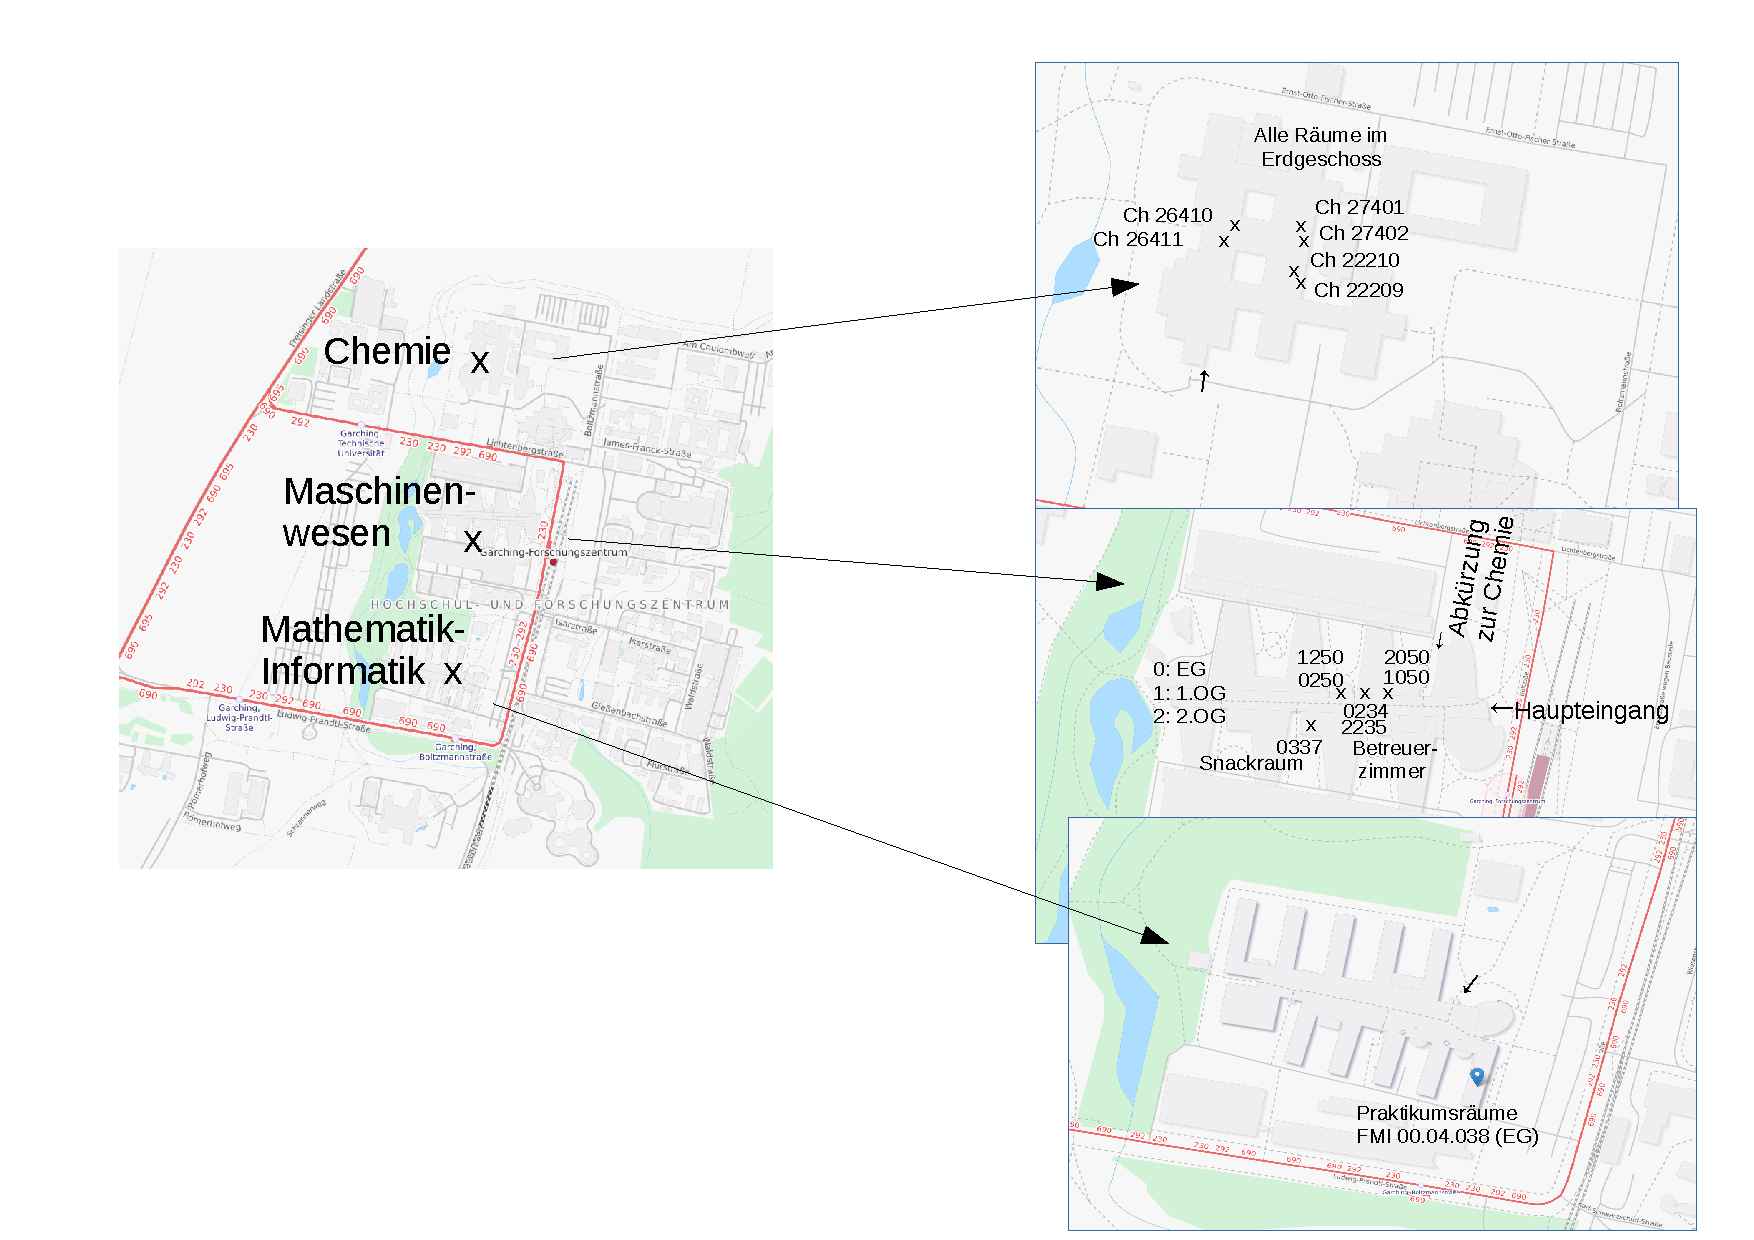
\includegraphics[scale=0.5]{campus_map.pdf}
\end{figure}
\newpage{}\begin{center}{\huge{}\textbf{Stundenplan von Celina Oberndörfer}}\end{center}\textbf{{\large{}Donnerstag}}\nopagebreak \\\begin{tabular} {|p{3cm} p{6cm} p{6cm}| }\hline \textbf{11:30 bis 13:45}&\textbf{Anreise zur TU München}&\textbf{Fakultät Maschinenwesen}\\\hline \textbf{12:00 bis 13:30}&\textbf{Mittagessen}&\textbf{Mensa Garching}\\\hline \textbf{14:00}&\textbf{Begrüßung}&\textbf{CH 26411}\\&Begrüßung, Besprechung des Zeitplans, Ausgabe der individuellen Stundenpläne,...&\\\hline \textbf{14:50 bis 16:20}&\textbf{Quanten- und Atomphysik I}&\textbf{CH 26410}\\&Betreuer: Ismail Achmed-Zade&ca. 28 Teilnehmer\\\hline \textbf{16:40 bis 18:10}&\textbf{Himmelsmechanik}&\textbf{MW 2050}\\&Betreuer: Lars Dehlwes&ca. 19 Teilnehmer\\\hline \textbf{18:30}&\textbf{Fahrt zur Jugendherberge}&\textbf{}\\\hline \textbf{19:00}&\textbf{Abendessen}&\textbf{Jugendherberge}\\\hline \end{tabular}\\\vspace{5.00000mm}~\\\textbf{{\large{}Freitag}}\nopagebreak \\\begin{tabular} {|p{3cm} p{6cm} p{6cm}| }\hline \textbf{06:30 bis 09:00}&\textbf{Frühstück}&\textbf{Jugendherberge}\\\hline \textbf{09:00 bis 13:00}&frei&\\\hline \textbf{13:00 bis 14:00}&\textbf{Mittagessen}&\textbf{Mensa Garching}\\\hline \textbf{14:20 bis 15:50}&\textbf{Kernphysik}&\textbf{MW 0250}\\&Betreuer: Johannes Rothe&ca. 18 Teilnehmer\\\hline \textbf{16:10 bis 17:40}&\textbf{Spezielle Relativitätstheorie}&\textbf{MW 1250}\\&Betreuer: Johannes Rothe&ca. 19 Teilnehmer\\\hline \textbf{18:00 bis 18:20}&\textbf{Erlebnisbericht IPhO}&\textbf{CH 26411}\\\hline \textbf{18:30}&\textbf{Fahrt zur Jugendherberge}&\textbf{}\\\hline \textbf{19:00}&\textbf{Abendessen}&\textbf{Jugendherberge}\\\hline \end{tabular}\\\vspace{5.00000mm}~\\\textbf{{\large{}Samstag}}\nopagebreak \\\begin{tabular} {|p{3cm} p{6cm} p{6cm}| }\hline \textbf{06:30 bis 08:00}&\textbf{Frühstück}&\textbf{Jugendherberge}\\\hline \textbf{08:00}&\textbf{Fahrt zur TU}&\textbf{}\\\hline \textbf{09:00 bis 10:30}&\textbf{Harmonische Schwingungen}&\textbf{MW 0250}\\&Betreuer: Ilja Göthel&ca. 9 Teilnehmer\\\hline \textbf{10:50 bis 12:20}&\textbf{Experiment Brennstoffzelle}&\textbf{Praktikum Brennstoffzelle}\\&Betreuer: Aaron Wild&ca. 6 Teilnehmer\\\hline \textbf{12:40 bis 14:00}&\textbf{Mittagessen}&\textbf{Fakultät Maschinenwesen}\\\hline \textbf{14:20 bis 15:50}&\textbf{Relativistische Teilchenphysik}&\textbf{CH 22210}\\&Betreuer: Lars Dehlwes&ca. 23 Teilnehmer\\\hline \textbf{16:10 bis 17:40}&\textbf{Quanten- und Atomphysik II}&\textbf{CH 22209}\\&Betreuer: Vitaly Andreev&ca. 28 Teilnehmer\\\hline \textbf{18:00 bis 18:20}&\textbf{Vorstellung GYPT}&\textbf{CH 26411}\\\hline \textbf{18:30}&\textbf{Fahrt zur Jugendherberge}&\textbf{}\\\hline \textbf{19:00}&\textbf{Abendessen}&\textbf{Jugendherberge}\\\hline \end{tabular}\\\vspace{5.00000mm}~\\\textbf{{\large{}Sonntag}}\nopagebreak \\\begin{tabular} {|p{3cm} p{6cm} p{6cm}| }\hline \textbf{06:30 bis 08:00}&\textbf{Frühstück}&\textbf{Jugendherberge}\\\hline \textbf{08:00}&\textbf{Fahrt zur TU}&\textbf{}\\\hline \textbf{09:00 bis 10:30}&\textbf{Gravitationsbeschleunigung}&\textbf{MW 1050}\\&Betreuer: Ann-Kathrin Raab&ca. 8 Teilnehmer\\\hline \textbf{10:50 bis 12:20}&\textbf{Aufgabenseminar Quanten- und Atomphysik und Struktur der Materie}&\textbf{MW 1250}\\&Betreuer: Vitaly Andreev&ca. 24 Teilnehmer\\\hline \textbf{12:40 bis 13:00}&\textbf{Verabschiedung}&\textbf{CH 26411}\\\hline \textbf{13:00}&\textbf{Individuelle Abreise}&\textbf{}\\\hline \textbf{13:00 bis 14:00}&\textbf{Mittagessen}&\textbf{}\\\hline \end{tabular}\\\vspace{5.00000mm}~\\
Notfallnummern: \\
Sven Jandura: xxxx xxxxxxxxx \\
Johannes Rothe: xxxx xxxxxxxxx \\

\large Hast du Lust, die Andern vom Seminar wiederzusehen?\\
\normalsize Dann komm doch einfach zum \textbf{Vereinstreffen}. Dazu musst du kein Vereinsmitglied sein. Neben interesannten Vorträgen und Exkursionen sind jede Menge Spiel und Spaß geplant. Schau in einem Monat einfach noch mal auf der Website vorbei. Wir freuen uns, wenn du dabei bist.

\begin{figure}[!h]
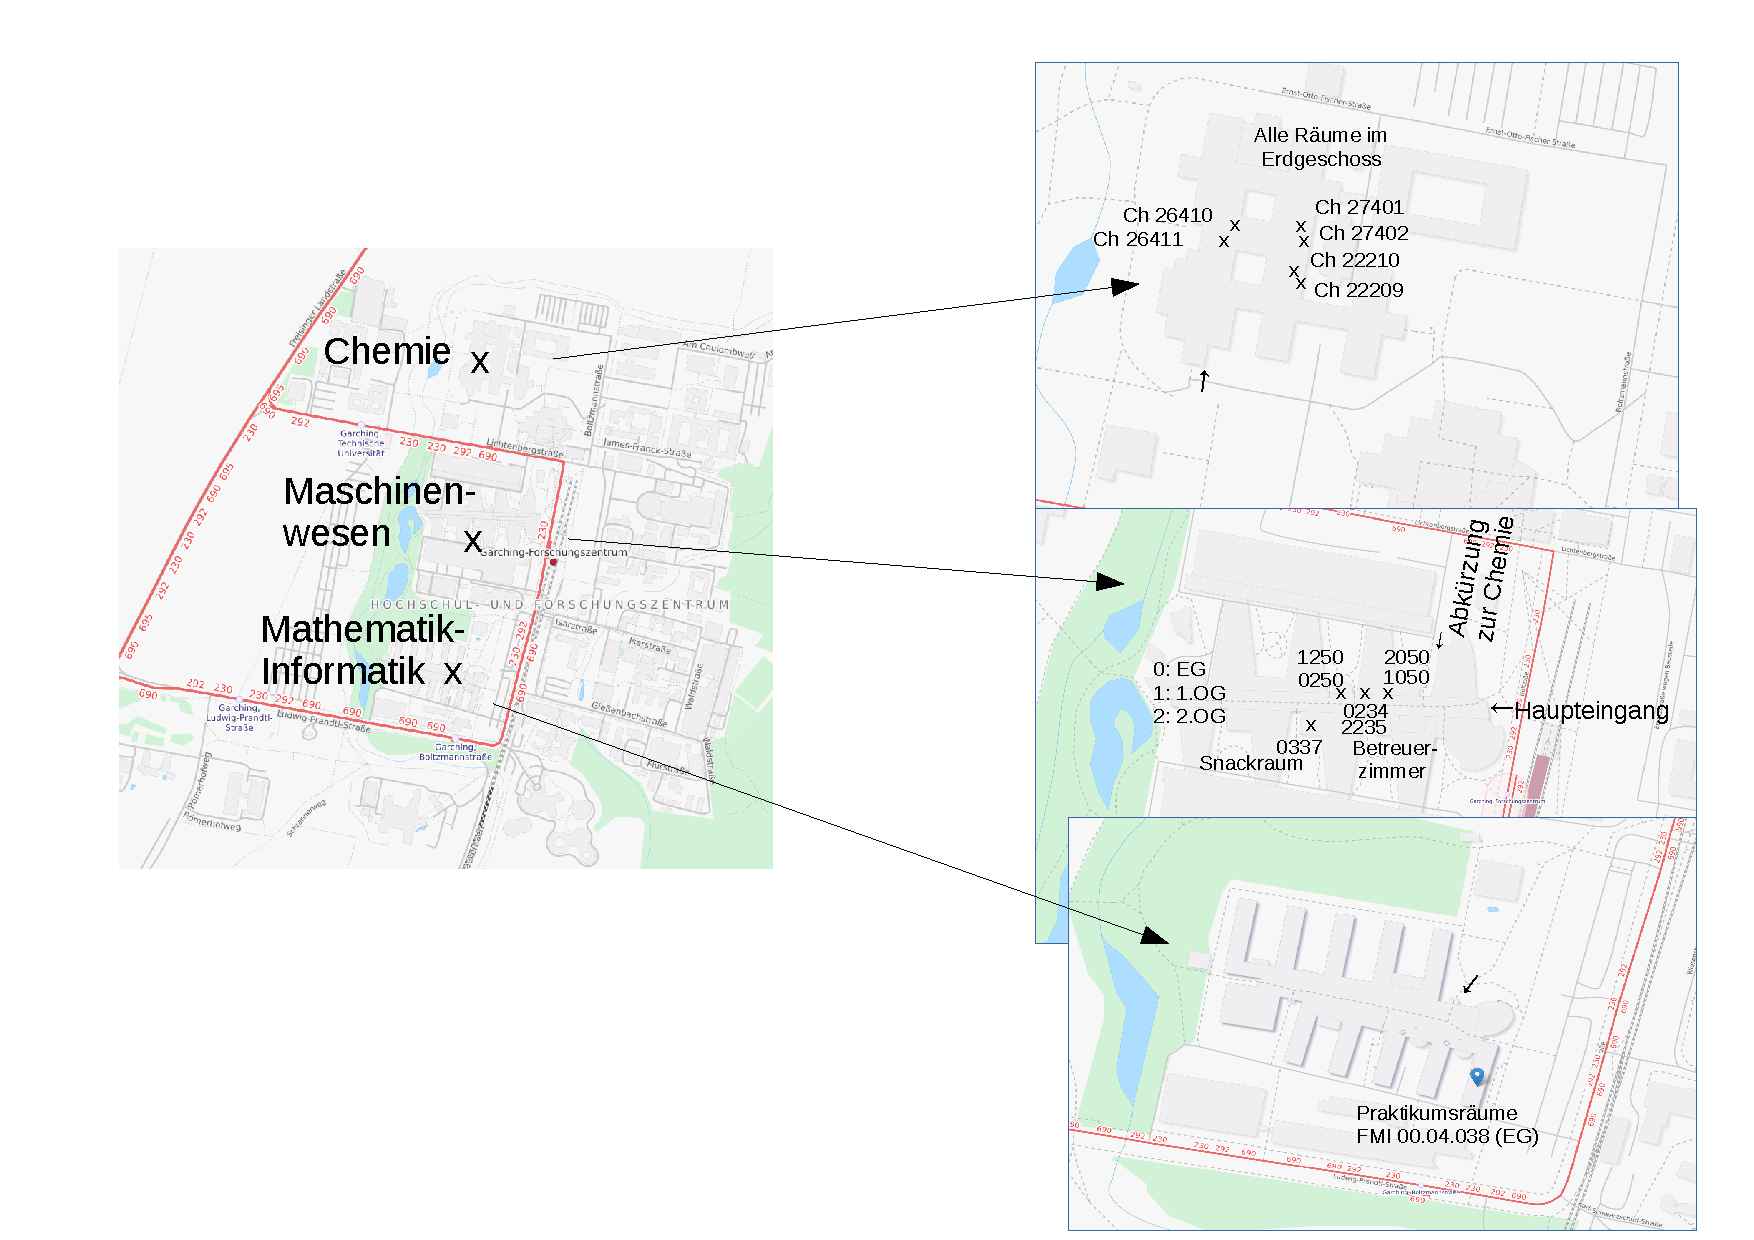
\includegraphics[scale=0.5]{campus_map.pdf}
\end{figure}
\newpage{}\begin{center}{\huge{}\textbf{Stundenplan von Charlotte Lange}}\end{center}\textbf{{\large{}Donnerstag}}\nopagebreak \\\begin{tabular} {|p{3cm} p{6cm} p{6cm}| }\hline \textbf{11:30 bis 13:45}&\textbf{Anreise zur TU München}&\textbf{Fakultät Maschinenwesen}\\\hline \textbf{12:00 bis 13:30}&\textbf{Mittagessen}&\textbf{Mensa Garching}\\\hline \textbf{14:00}&\textbf{Begrüßung}&\textbf{CH 26411}\\&Begrüßung, Besprechung des Zeitplans, Ausgabe der individuellen Stundenpläne,...&\\\hline \textbf{14:50 bis 16:20}&\textbf{Elektrische Schaltungen}&\textbf{MW 0250}\\&Betreuer: Christopher Pfeiffer&ca. 16 Teilnehmer\\\hline \textbf{16:40 bis 18:10}&\textbf{Klassische Mechanik}&\textbf{MW 1250}\\&Betreuer: Maximilian Marienhagen&ca. 10 Teilnehmer\\\hline \textbf{18:30}&\textbf{Fahrt zur Jugendherberge}&\textbf{}\\\hline \textbf{19:00}&\textbf{Abendessen}&\textbf{Jugendherberge}\\\hline \end{tabular}\\\vspace{5.00000mm}~\\\textbf{{\large{}Freitag}}\nopagebreak \\\begin{tabular} {|p{3cm} p{6cm} p{6cm}| }\hline \textbf{06:30 bis 09:00}&\textbf{Frühstück}&\textbf{Jugendherberge}\\\hline \textbf{09:00 bis 13:00}&\textbf{Besichtigung der Forschungsneutronenquelle FRM II}&\textbf{MW 2050}\\&Betreuer: Felix Wechsler&ca. 28 Teilnehmer\\\hline \textbf{13:00 bis 14:00}&\textbf{Mittagessen}&\textbf{Mensa Garching}\\\hline \textbf{14:20 bis 15:50}&\textbf{Gewöhnliche Differentialgleichungen}&\textbf{MW 1250}\\&Betreuer: Sven Jandura&ca. 20 Teilnehmer\\\hline \textbf{16:10 bis 17:40}&\textbf{Näherungsmethoden}&\textbf{CH 26410}\\&Betreuer: Vincent Grande&ca. 11 Teilnehmer\\\hline \textbf{18:00 bis 18:20}&\textbf{Erlebnisbericht IPhO}&\textbf{CH 26411}\\\hline \textbf{18:30}&\textbf{Fahrt zur Jugendherberge}&\textbf{}\\\hline \textbf{19:00}&\textbf{Abendessen}&\textbf{Jugendherberge}\\\hline \end{tabular}\\\vspace{5.00000mm}~\\\textbf{{\large{}Samstag}}\nopagebreak \\\begin{tabular} {|p{3cm} p{6cm} p{6cm}| }\hline \textbf{06:30 bis 08:00}&\textbf{Frühstück}&\textbf{Jugendherberge}\\\hline \textbf{08:00}&\textbf{Fahrt zur TU}&\textbf{}\\\hline \textbf{09:00 bis 10:30}&\textbf{Elektrodynamik 1}&\textbf{MW 1250}\\&Betreuer: Maximilian Keitel&ca. 21 Teilnehmer\\\hline \textbf{10:50 bis 12:20}&\textbf{Elektrodynamik 2}&\textbf{MW 1250}\\&Betreuer: Maximilian Keitel&ca. 21 Teilnehmer\\\hline \textbf{12:40 bis 14:00}&\textbf{Mittagessen}&\textbf{Fakultät Maschinenwesen}\\\hline \textbf{14:20 bis 15:50}&\textbf{Quanten- und Atomphysik I}&\textbf{CH 22209}\\&Betreuer: Vitaly Andreev&ca. 22 Teilnehmer\\\hline \textbf{16:10 bis 17:40}&\textbf{Quanten- und Atomphysik II}&\textbf{CH 22209}\\&Betreuer: Vitaly Andreev&ca. 28 Teilnehmer\\\hline \textbf{18:00 bis 18:20}&\textbf{Vorstellung GYPT}&\textbf{CH 26411}\\\hline \textbf{18:30}&\textbf{Fahrt zur Jugendherberge}&\textbf{}\\\hline \textbf{19:00}&\textbf{Abendessen}&\textbf{Jugendherberge}\\\hline \end{tabular}\\\vspace{5.00000mm}~\\\textbf{{\large{}Sonntag}}\nopagebreak \\\begin{tabular} {|p{3cm} p{6cm} p{6cm}| }\hline \textbf{06:30 bis 08:00}&\textbf{Frühstück}&\textbf{Jugendherberge}\\\hline \textbf{08:00}&\textbf{Fahrt zur TU}&\textbf{}\\\hline \textbf{09:00 bis 10:30}&\textbf{Elektronik}&\textbf{CH 26410}\\&Betreuer: Martin Großhauser&ca. 10 Teilnehmer\\\hline \textbf{10:50 bis 12:20}&\textbf{Wellenoptik}&\textbf{MW 0250}\\&Betreuer: Christopher Pfeiffer&ca. 12 Teilnehmer\\\hline \textbf{12:40 bis 13:00}&\textbf{Verabschiedung}&\textbf{CH 26411}\\\hline \textbf{13:00}&\textbf{Individuelle Abreise}&\textbf{}\\\hline \textbf{13:00 bis 14:00}&\textbf{Mittagessen}&\textbf{}\\\hline \end{tabular}\\\vspace{5.00000mm}~\\
Notfallnummern: \\
Sven Jandura: xxxx xxxxxxxxx \\
Johannes Rothe: xxxx xxxxxxxxx \\

\large Hast du Lust, die Andern vom Seminar wiederzusehen?\\
\normalsize Dann komm doch einfach zum \textbf{Vereinstreffen}. Dazu musst du kein Vereinsmitglied sein. Neben interesannten Vorträgen und Exkursionen sind jede Menge Spiel und Spaß geplant. Schau in einem Monat einfach noch mal auf der Website vorbei. Wir freuen uns, wenn du dabei bist.

\begin{figure}[!h]
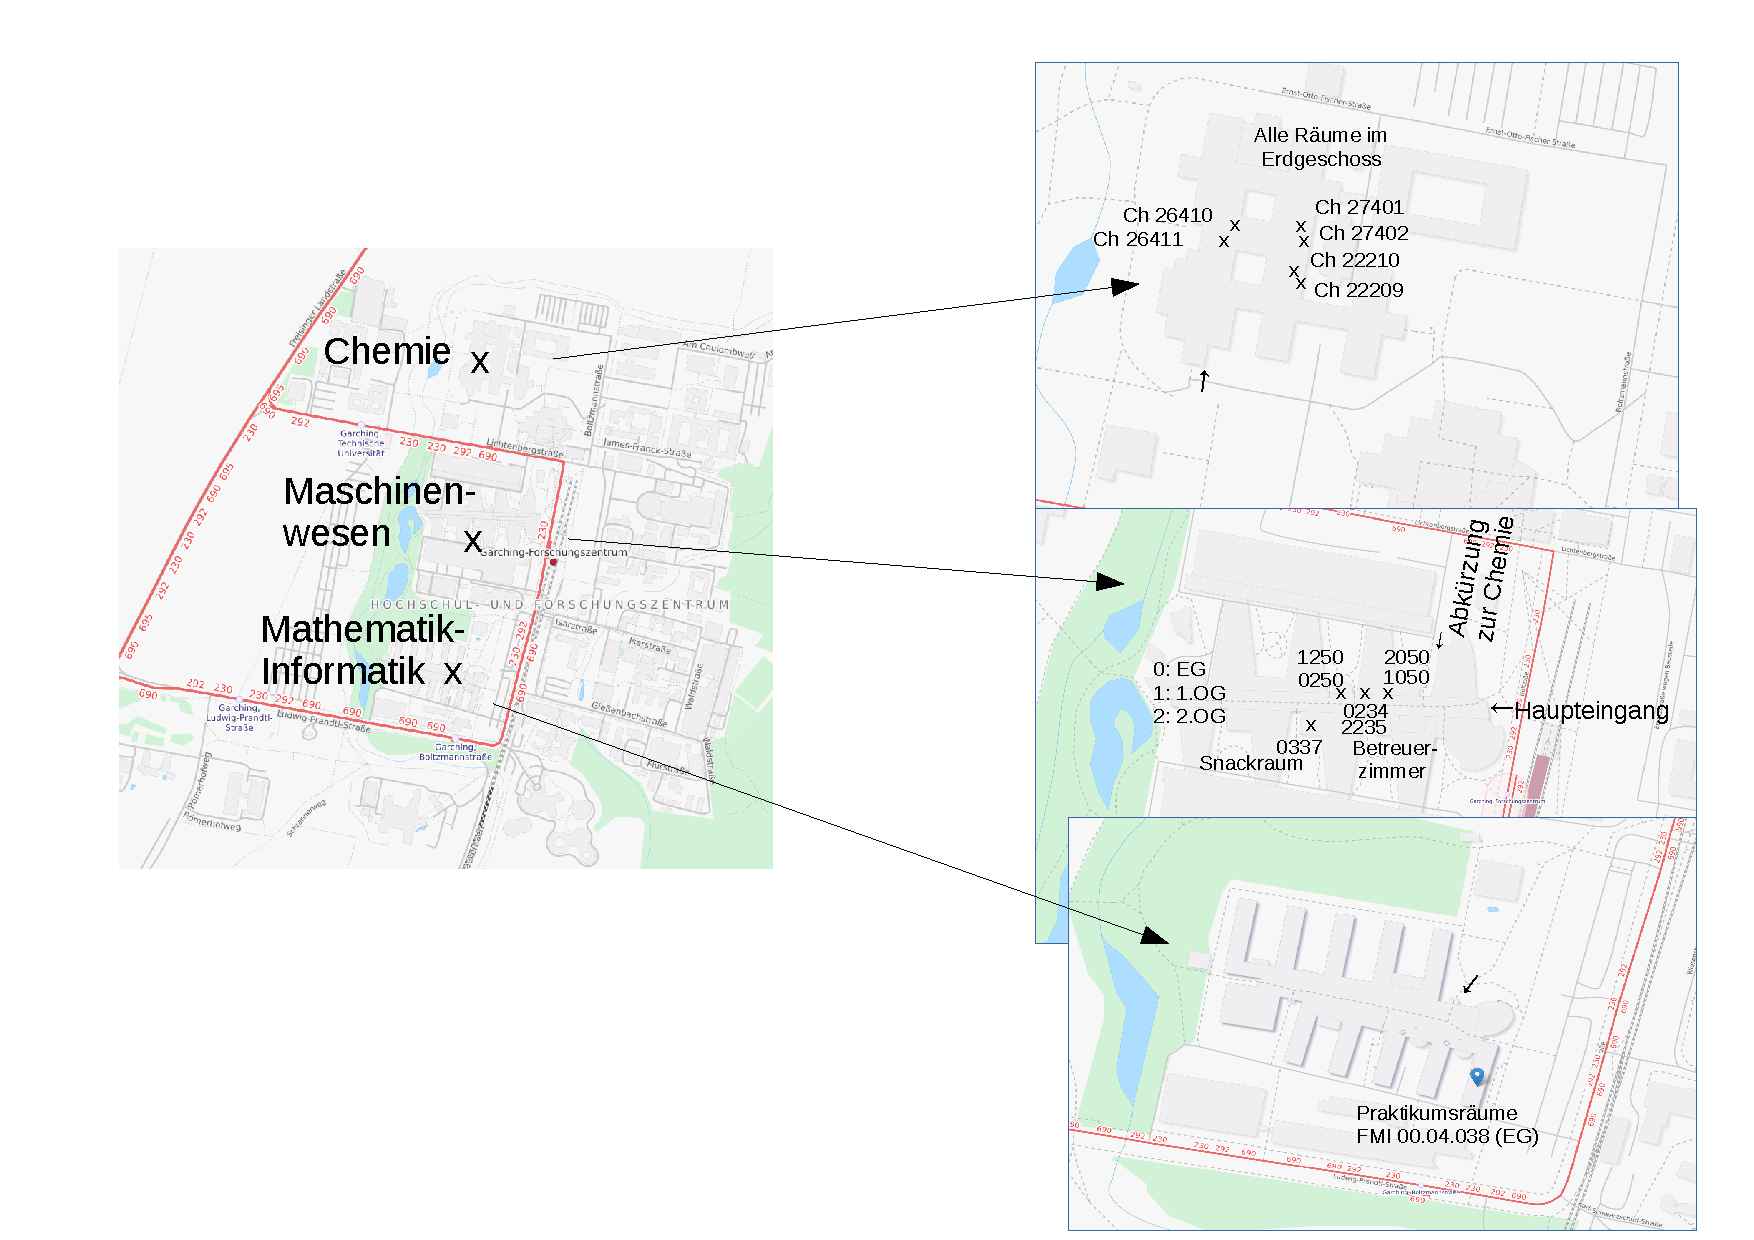
\includegraphics[scale=0.5]{campus_map.pdf}
\end{figure}
\newpage{}\begin{center}{\huge{}\textbf{Stundenplan von Christiane Mayer}}\end{center}\textbf{{\large{}Donnerstag}}\nopagebreak \\\begin{tabular} {|p{3cm} p{6cm} p{6cm}| }\hline \textbf{11:30 bis 13:45}&\textbf{Anreise zur TU München}&\textbf{Fakultät Maschinenwesen}\\\hline \textbf{12:00 bis 13:30}&\textbf{Mittagessen}&\textbf{Mensa Garching}\\\hline \textbf{14:00}&\textbf{Begrüßung}&\textbf{CH 26411}\\&Begrüßung, Besprechung des Zeitplans, Ausgabe der individuellen Stundenpläne,...&\\\hline \textbf{14:50 bis 16:20}&\textbf{Quanten- und Atomphysik I}&\textbf{CH 26410}\\&Betreuer: Ismail Achmed-Zade&ca. 28 Teilnehmer\\\hline \textbf{16:40 bis 18:10}&\textbf{Himmelsmechanik}&\textbf{MW 2050}\\&Betreuer: Lars Dehlwes&ca. 19 Teilnehmer\\\hline \textbf{18:30}&\textbf{Fahrt zur Jugendherberge}&\textbf{}\\\hline \textbf{19:00}&\textbf{Abendessen}&\textbf{Jugendherberge}\\\hline \end{tabular}\\\vspace{5.00000mm}~\\\textbf{{\large{}Freitag}}\nopagebreak \\\begin{tabular} {|p{3cm} p{6cm} p{6cm}| }\hline \textbf{06:30 bis 09:00}&\textbf{Frühstück}&\textbf{Jugendherberge}\\\hline \textbf{09:00 bis 13:00}&frei&\\\hline \textbf{13:00 bis 14:00}&\textbf{Mittagessen}&\textbf{Mensa Garching}\\\hline \textbf{14:20 bis 15:50}&\textbf{Experiment spezifische Elektronenladung}&\textbf{Praktikum spezifische Elektronenladung}\\&Betreuer: Felix Wechsler&ca. 6 Teilnehmer\\\hline \textbf{16:10 bis 17:40}&\textbf{Spezielle Relativitätstheorie}&\textbf{MW 1250}\\&Betreuer: Johannes Rothe&ca. 19 Teilnehmer\\\hline \textbf{18:00 bis 18:20}&\textbf{Erlebnisbericht IPhO}&\textbf{CH 26411}\\\hline \textbf{18:30}&\textbf{Fahrt zur Jugendherberge}&\textbf{}\\\hline \textbf{19:00}&\textbf{Abendessen}&\textbf{Jugendherberge}\\\hline \end{tabular}\\\vspace{5.00000mm}~\\\textbf{{\large{}Samstag}}\nopagebreak \\\begin{tabular} {|p{3cm} p{6cm} p{6cm}| }\hline \textbf{06:30 bis 08:00}&\textbf{Frühstück}&\textbf{Jugendherberge}\\\hline \textbf{08:00}&\textbf{Fahrt zur TU}&\textbf{}\\\hline \textbf{09:00 bis 10:30}&\textbf{Experimentieren und Auswerten}&\textbf{CH 26411}\\&Betreuer: Ann-Kathrin Raab&ca. 18 Teilnehmer\\\hline \textbf{10:50 bis 12:20}&\textbf{Experiment Millikan-Versuch}&\textbf{Praktikum Millikan-Versuch}\\&Betreuer: Samuel Moll&ca. 6 Teilnehmer\\\hline \textbf{12:40 bis 14:00}&\textbf{Mittagessen}&\textbf{Fakultät Maschinenwesen}\\\hline \textbf{14:20 bis 15:50}&\textbf{Relativistische Teilchenphysik}&\textbf{CH 22210}\\&Betreuer: Lars Dehlwes&ca. 23 Teilnehmer\\\hline \textbf{16:10 bis 17:40}&\textbf{Elektrische Blackboxen}&\textbf{Praktikum Blackboxen}\\&Betreuer: Eugen Dizer&ca. 6 Teilnehmer\\\hline \textbf{18:00 bis 18:20}&\textbf{Vorstellung GYPT}&\textbf{CH 26411}\\\hline \textbf{18:30}&\textbf{Fahrt zur Jugendherberge}&\textbf{}\\\hline \textbf{19:00}&\textbf{Abendessen}&\textbf{Jugendherberge}\\\hline \end{tabular}\\\vspace{5.00000mm}~\\\textbf{{\large{}Sonntag}}\nopagebreak \\\begin{tabular} {|p{3cm} p{6cm} p{6cm}| }\hline \textbf{06:30 bis 08:00}&\textbf{Frühstück}&\textbf{Jugendherberge}\\\hline \textbf{08:00}&\textbf{Fahrt zur TU}&\textbf{}\\\hline \textbf{09:00 bis 10:30}&\textbf{Quanten- und Atomphysik II}&\textbf{MW 1250}\\&Betreuer: Vitaly Andreev&ca. 15 Teilnehmer\\\hline \textbf{10:50 bis 12:20}&\textbf{Aufgabenseminar Quanten- und Atomphysik und Struktur der Materie}&\textbf{MW 1250}\\&Betreuer: Vitaly Andreev&ca. 24 Teilnehmer\\\hline \textbf{12:40 bis 13:00}&\textbf{Verabschiedung}&\textbf{CH 26411}\\\hline \textbf{13:00}&\textbf{Individuelle Abreise}&\textbf{}\\\hline \textbf{13:00 bis 14:00}&\textbf{Mittagessen}&\textbf{}\\\hline \end{tabular}\\\vspace{5.00000mm}~\\
Notfallnummern: \\
Sven Jandura: xxxx xxxxxxxxx \\
Johannes Rothe: xxxx xxxxxxxxx \\

\large Hast du Lust, die Andern vom Seminar wiederzusehen?\\
\normalsize Dann komm doch einfach zum \textbf{Vereinstreffen}. Dazu musst du kein Vereinsmitglied sein. Neben interesannten Vorträgen und Exkursionen sind jede Menge Spiel und Spaß geplant. Schau in einem Monat einfach noch mal auf der Website vorbei. Wir freuen uns, wenn du dabei bist.

\begin{figure}[!h]
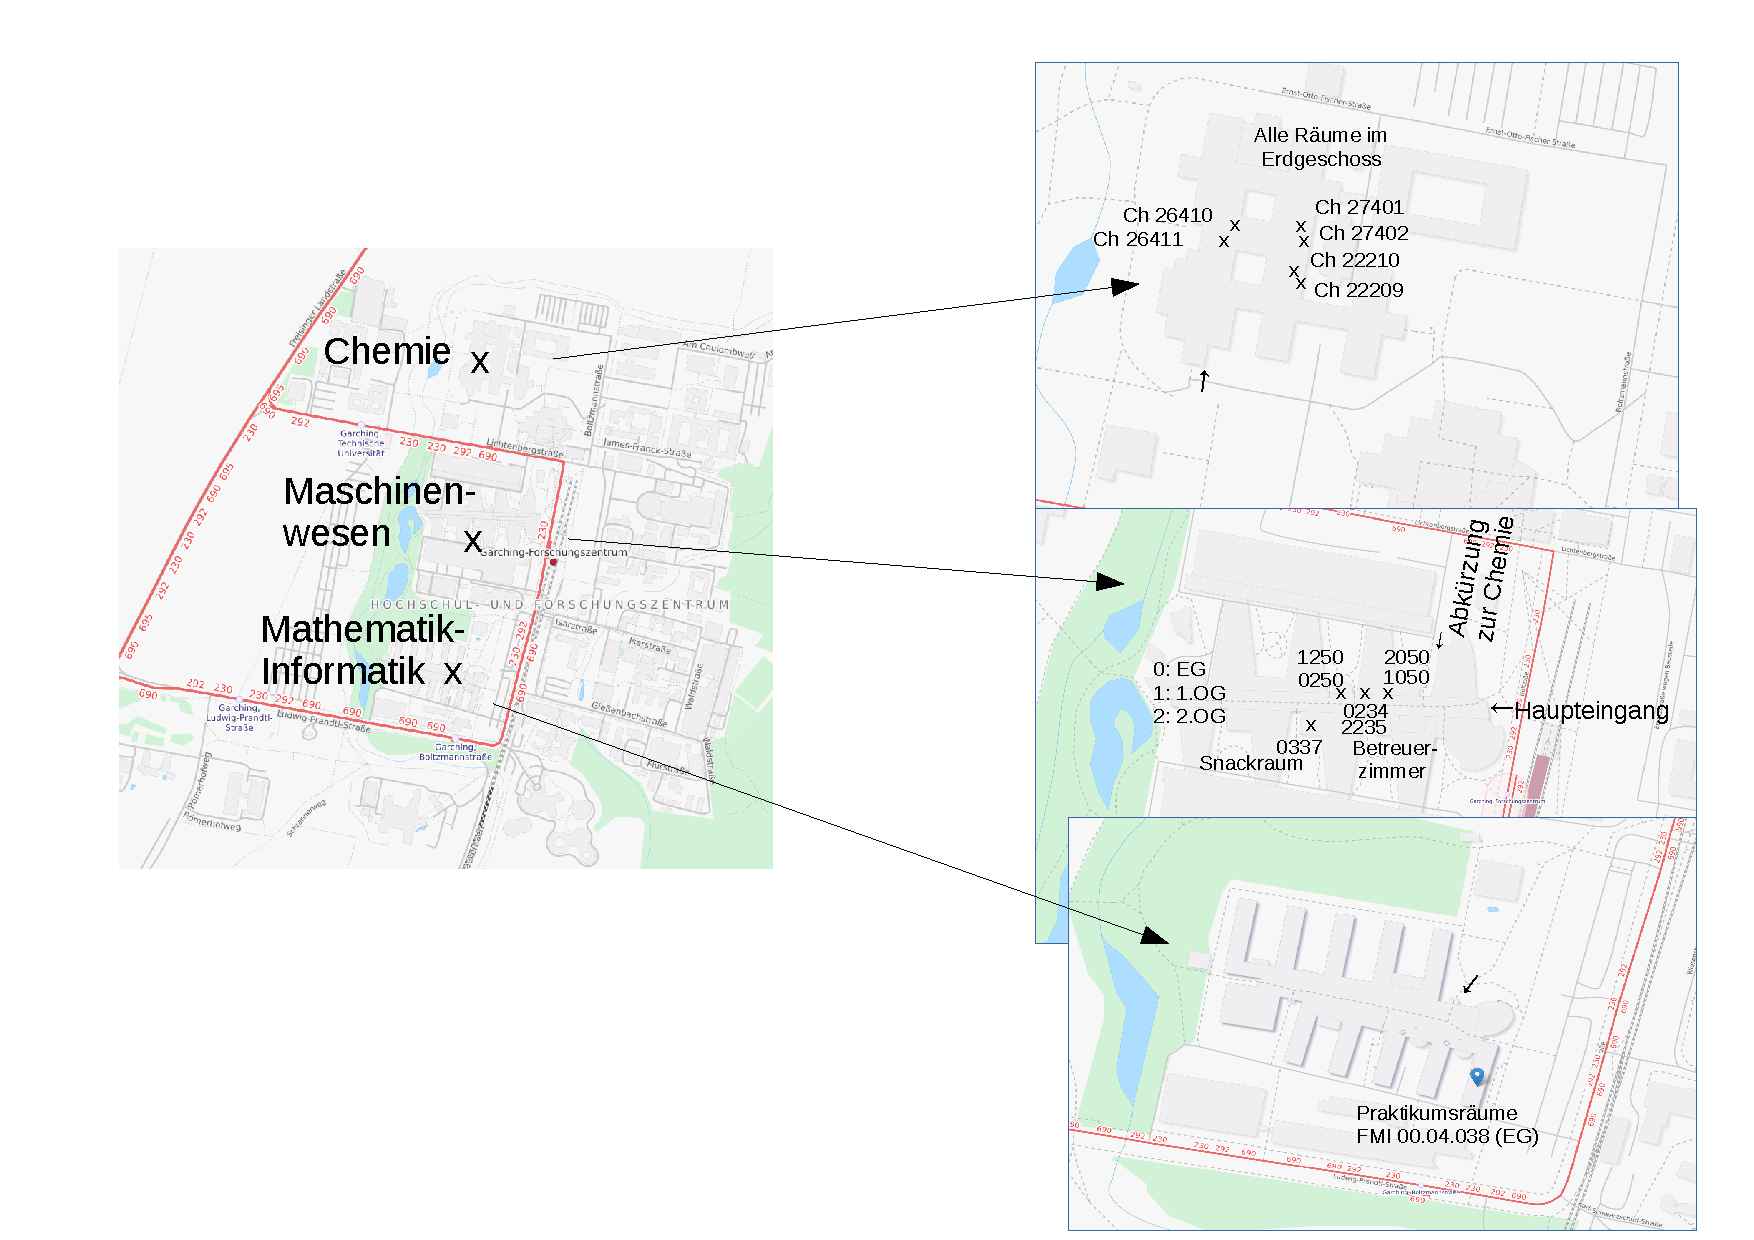
\includegraphics[scale=0.5]{campus_map.pdf}
\end{figure}
\newpage{}\begin{center}{\huge{}\textbf{Stundenplan von Daniel Samoylov}}\end{center}\textbf{{\large{}Donnerstag}}\nopagebreak \\\begin{tabular} {|p{3cm} p{6cm} p{6cm}| }\hline \textbf{11:30 bis 13:45}&\textbf{Anreise zur TU München}&\textbf{Fakultät Maschinenwesen}\\\hline \textbf{12:00 bis 13:30}&\textbf{Mittagessen}&\textbf{Mensa Garching}\\\hline \textbf{14:00}&\textbf{Begrüßung}&\textbf{CH 26411}\\&Begrüßung, Besprechung des Zeitplans, Ausgabe der individuellen Stundenpläne,...&\\\hline \textbf{14:50 bis 16:20}&\textbf{Elektrische Schaltungen}&\textbf{MW 0250}\\&Betreuer: Christopher Pfeiffer&ca. 16 Teilnehmer\\\hline \textbf{16:40 bis 18:10}&\textbf{Einführung ins Integrieren}&\textbf{MW 1050}\\&Betreuer: Johannes Rothe&ca. 14 Teilnehmer\\\hline \textbf{18:30}&\textbf{Fahrt zur Jugendherberge}&\textbf{}\\\hline \textbf{19:00}&\textbf{Abendessen}&\textbf{Jugendherberge}\\\hline \end{tabular}\\\vspace{5.00000mm}~\\\textbf{{\large{}Freitag}}\nopagebreak \\\begin{tabular} {|p{3cm} p{6cm} p{6cm}| }\hline \textbf{06:30 bis 09:00}&\textbf{Frühstück}&\textbf{Jugendherberge}\\\hline \textbf{09:00 bis 13:00}&frei&\\\hline \textbf{13:00 bis 14:00}&\textbf{Mittagessen}&\textbf{Mensa Garching}\\\hline \textbf{14:20 bis 15:50}&\textbf{Experiment Oszilloskop}&\textbf{Praktikum Oszilloskop}\\&Betreuer: Christopher Pfeiffer&ca. 6 Teilnehmer\\\hline \textbf{16:10 bis 17:40}&\textbf{Experiment Magnetismus}&\textbf{Praktikum Magnetismus}\\&Betreuer: Lars Dehlwes&ca. 6 Teilnehmer\\\hline \textbf{18:00 bis 18:20}&\textbf{Erlebnisbericht IPhO}&\textbf{CH 26411}\\\hline \textbf{18:30}&\textbf{Fahrt zur Jugendherberge}&\textbf{}\\\hline \textbf{19:00}&\textbf{Abendessen}&\textbf{Jugendherberge}\\\hline \end{tabular}\\\vspace{5.00000mm}~\\\textbf{{\large{}Samstag}}\nopagebreak \\\begin{tabular} {|p{3cm} p{6cm} p{6cm}| }\hline \textbf{06:30 bis 08:00}&\textbf{Frühstück}&\textbf{Jugendherberge}\\\hline \textbf{08:00}&\textbf{Fahrt zur TU}&\textbf{}\\\hline \textbf{09:00 bis 10:30}&\textbf{Thermodynamik 2 - Statistische Physik}&\textbf{MW 1050}\\&Betreuer: Vitaly Andreev&ca. 17 Teilnehmer\\\hline \textbf{10:50 bis 12:20}&\textbf{Elektrodynamik 2}&\textbf{MW 1250}\\&Betreuer: Maximilian Keitel&ca. 21 Teilnehmer\\\hline \textbf{12:40 bis 14:00}&\textbf{Mittagessen}&\textbf{Fakultät Maschinenwesen}\\\hline \textbf{14:20 bis 15:50}&\textbf{Quanten- und Atomphysik I}&\textbf{CH 22209}\\&Betreuer: Vitaly Andreev&ca. 22 Teilnehmer\\\hline \textbf{16:10 bis 17:40}&\textbf{Komplexe Wechselstromrechnung}&\textbf{MW 0250}\\&Betreuer: Vincent Grande&ca. 13 Teilnehmer\\\hline \textbf{18:00 bis 18:20}&\textbf{Vorstellung GYPT}&\textbf{CH 26411}\\\hline \textbf{18:30}&\textbf{Fahrt zur Jugendherberge}&\textbf{}\\\hline \textbf{19:00}&\textbf{Abendessen}&\textbf{Jugendherberge}\\\hline \end{tabular}\\\vspace{5.00000mm}~\\\textbf{{\large{}Sonntag}}\nopagebreak \\\begin{tabular} {|p{3cm} p{6cm} p{6cm}| }\hline \textbf{06:30 bis 08:00}&\textbf{Frühstück}&\textbf{Jugendherberge}\\\hline \textbf{08:00}&\textbf{Fahrt zur TU}&\textbf{}\\\hline \textbf{09:00 bis 10:30}&\textbf{Elektronik}&\textbf{CH 26410}\\&Betreuer: Martin Großhauser&ca. 10 Teilnehmer\\\hline \textbf{10:50 bis 12:20}&\textbf{Relativistische Teilchenphysik}&\textbf{CH 22210}\\&Betreuer: Lars Dehlwes&ca. 11 Teilnehmer\\\hline \textbf{12:40 bis 13:00}&\textbf{Verabschiedung}&\textbf{CH 26411}\\\hline \textbf{13:00}&\textbf{Individuelle Abreise}&\textbf{}\\\hline \textbf{13:00 bis 14:00}&\textbf{Mittagessen}&\textbf{}\\\hline \end{tabular}\\\vspace{5.00000mm}~\\
Notfallnummern: \\
Sven Jandura: xxxx xxxxxxxxx \\
Johannes Rothe: xxxx xxxxxxxxx \\

\large Hast du Lust, die Andern vom Seminar wiederzusehen?\\
\normalsize Dann komm doch einfach zum \textbf{Vereinstreffen}. Dazu musst du kein Vereinsmitglied sein. Neben interesannten Vorträgen und Exkursionen sind jede Menge Spiel und Spaß geplant. Schau in einem Monat einfach noch mal auf der Website vorbei. Wir freuen uns, wenn du dabei bist.

\begin{figure}[!h]
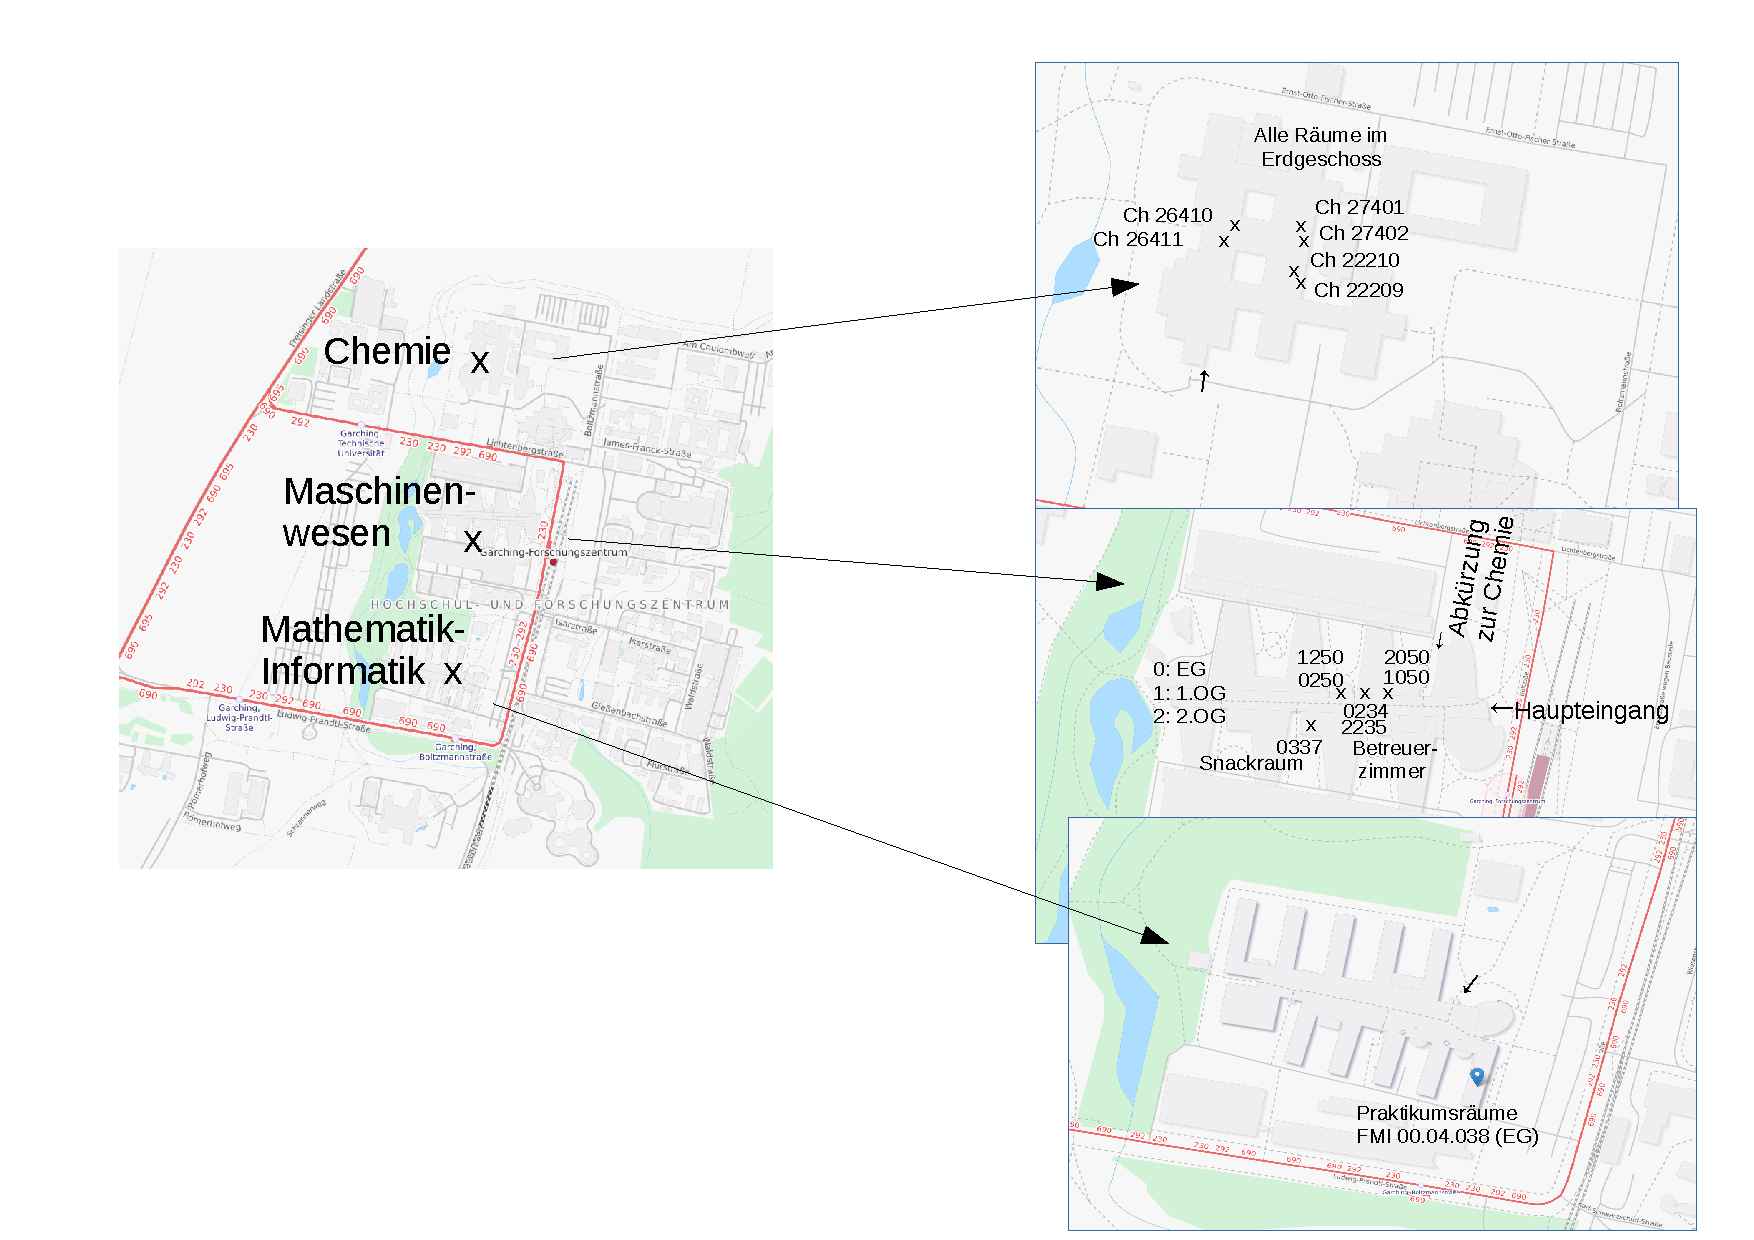
\includegraphics[scale=0.5]{campus_map.pdf}
\end{figure}
\newpage{}\begin{center}{\huge{}\textbf{Stundenplan von David Danhofer}}\end{center}\textbf{{\large{}Donnerstag}}\nopagebreak \\\begin{tabular} {|p{3cm} p{6cm} p{6cm}| }\hline \textbf{11:30 bis 13:45}&\textbf{Anreise zur TU München}&\textbf{Fakultät Maschinenwesen}\\\hline \textbf{12:00 bis 13:30}&\textbf{Mittagessen}&\textbf{Mensa Garching}\\\hline \textbf{14:00}&\textbf{Begrüßung}&\textbf{CH 26411}\\&Begrüßung, Besprechung des Zeitplans, Ausgabe der individuellen Stundenpläne,...&\\\hline \textbf{14:50 bis 16:20}&\textbf{Experimentieren und Auswerten}&\textbf{CH 26411}\\&Betreuer: Ann-Kathrin Raab&ca. 18 Teilnehmer\\\hline \textbf{16:40 bis 18:10}&\textbf{Näherungsmethoden}&\textbf{MW 0234}\\&Betreuer: Ilja Göthel&ca. 13 Teilnehmer\\\hline \textbf{18:30}&\textbf{Fahrt zur Jugendherberge}&\textbf{}\\\hline \textbf{19:00}&\textbf{Abendessen}&\textbf{Jugendherberge}\\\hline \end{tabular}\\\vspace{5.00000mm}~\\\textbf{{\large{}Freitag}}\nopagebreak \\\begin{tabular} {|p{3cm} p{6cm} p{6cm}| }\hline \textbf{06:30 bis 09:00}&\textbf{Frühstück}&\textbf{Jugendherberge}\\\hline \textbf{09:00 bis 13:00}&frei&\\\hline \textbf{13:00 bis 14:00}&\textbf{Mittagessen}&\textbf{Mensa Garching}\\\hline \textbf{14:20 bis 15:50}&\textbf{Experiment Brückenschaltung}&\textbf{Praktikum Brückenschaltung}\\&Betreuer: Martin Großhauser&ca. 6 Teilnehmer\\\hline \textbf{16:10 bis 17:40}&\textbf{Spezielle Relativitätstheorie}&\textbf{MW 1250}\\&Betreuer: Johannes Rothe&ca. 19 Teilnehmer\\\hline \textbf{18:00 bis 18:20}&\textbf{Erlebnisbericht IPhO}&\textbf{CH 26411}\\\hline \textbf{18:30}&\textbf{Fahrt zur Jugendherberge}&\textbf{}\\\hline \textbf{19:00}&\textbf{Abendessen}&\textbf{Jugendherberge}\\\hline \end{tabular}\\\vspace{5.00000mm}~\\\textbf{{\large{}Samstag}}\nopagebreak \\\begin{tabular} {|p{3cm} p{6cm} p{6cm}| }\hline \textbf{06:30 bis 08:00}&\textbf{Frühstück}&\textbf{Jugendherberge}\\\hline \textbf{08:00}&\textbf{Fahrt zur TU}&\textbf{}\\\hline \textbf{09:00 bis 10:30}&\textbf{Elektrodynamik 1}&\textbf{MW 1250}\\&Betreuer: Maximilian Keitel&ca. 21 Teilnehmer\\\hline \textbf{10:50 bis 12:20}&\textbf{Elektrodynamik 2}&\textbf{MW 1250}\\&Betreuer: Maximilian Keitel&ca. 21 Teilnehmer\\\hline \textbf{12:40 bis 14:00}&\textbf{Mittagessen}&\textbf{Fakultät Maschinenwesen}\\\hline \textbf{14:20 bis 15:50}&\textbf{Quanten- und Atomphysik I}&\textbf{CH 22209}\\&Betreuer: Vitaly Andreev&ca. 22 Teilnehmer\\\hline \textbf{16:10 bis 17:40}&\textbf{Aufgabenseminar Elektrodynamik}&\textbf{MW 1250}\\&Betreuer: Maximilian Keitel&ca. 8 Teilnehmer\\\hline \textbf{18:00 bis 18:20}&\textbf{Vorstellung GYPT}&\textbf{CH 26411}\\\hline \textbf{18:30}&\textbf{Fahrt zur Jugendherberge}&\textbf{}\\\hline \textbf{19:00}&\textbf{Abendessen}&\textbf{Jugendherberge}\\\hline \end{tabular}\\\vspace{5.00000mm}~\\\textbf{{\large{}Sonntag}}\nopagebreak \\\begin{tabular} {|p{3cm} p{6cm} p{6cm}| }\hline \textbf{06:30 bis 08:00}&\textbf{Frühstück}&\textbf{Jugendherberge}\\\hline \textbf{08:00}&\textbf{Fahrt zur TU}&\textbf{}\\\hline \textbf{09:00 bis 10:30}&\textbf{Aufgabenseminar Wärmelehre}&\textbf{CH 22209}\\&Betreuer: Maximilian Marienhagen&ca. 9 Teilnehmer\\\hline \textbf{10:50 bis 12:20}&\textbf{Elektrische Blackboxen}&\textbf{Praktikum Blackboxen}\\&Betreuer: Eugen Dizer&ca. 6 Teilnehmer\\\hline \textbf{12:40 bis 13:00}&\textbf{Verabschiedung}&\textbf{CH 26411}\\\hline \textbf{13:00}&\textbf{Individuelle Abreise}&\textbf{}\\\hline \textbf{13:00 bis 14:00}&\textbf{Mittagessen}&\textbf{}\\\hline \end{tabular}\\\vspace{5.00000mm}~\\
Notfallnummern: \\
Sven Jandura: xxxx xxxxxxxxx \\
Johannes Rothe: xxxx xxxxxxxxx \\

\large Hast du Lust, die Andern vom Seminar wiederzusehen?\\
\normalsize Dann komm doch einfach zum \textbf{Vereinstreffen}. Dazu musst du kein Vereinsmitglied sein. Neben interesannten Vorträgen und Exkursionen sind jede Menge Spiel und Spaß geplant. Schau in einem Monat einfach noch mal auf der Website vorbei. Wir freuen uns, wenn du dabei bist.

\begin{figure}[!h]
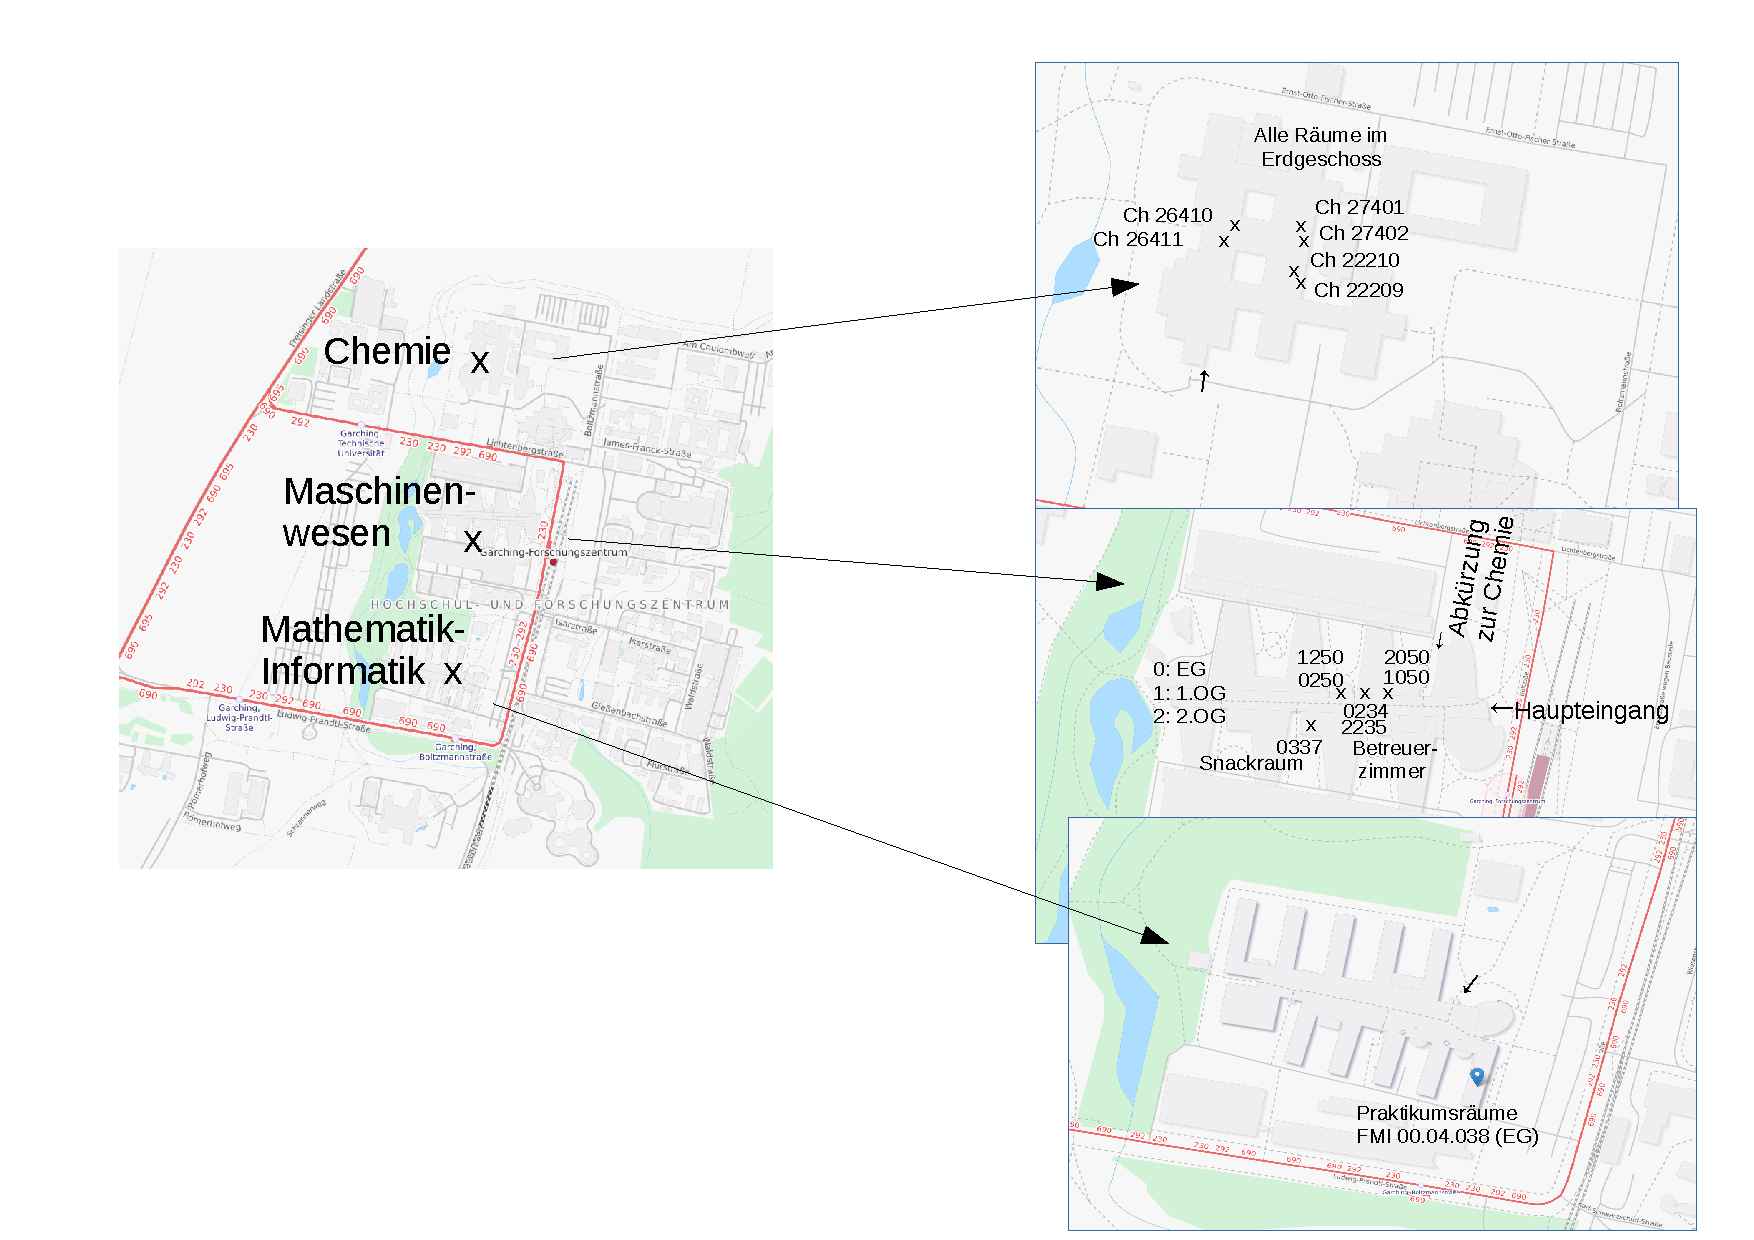
\includegraphics[scale=0.5]{campus_map.pdf}
\end{figure}
\newpage{}\begin{center}{\huge{}\textbf{Stundenplan von David Ventzke}}\end{center}\textbf{{\large{}Donnerstag}}\nopagebreak \\\begin{tabular} {|p{3cm} p{6cm} p{6cm}| }\hline \textbf{11:30 bis 13:45}&\textbf{Anreise zur TU München}&\textbf{Fakultät Maschinenwesen}\\\hline \textbf{12:00 bis 13:30}&\textbf{Mittagessen}&\textbf{Mensa Garching}\\\hline \textbf{14:00}&\textbf{Begrüßung}&\textbf{CH 26411}\\&Begrüßung, Besprechung des Zeitplans, Ausgabe der individuellen Stundenpläne,...&\\\hline \textbf{14:50 bis 16:20}&\textbf{Quanten- und Atomphysik I}&\textbf{CH 26410}\\&Betreuer: Ismail Achmed-Zade&ca. 28 Teilnehmer\\\hline \textbf{16:40 bis 18:10}&\textbf{Himmelsmechanik}&\textbf{MW 2050}\\&Betreuer: Lars Dehlwes&ca. 19 Teilnehmer\\\hline \textbf{18:30}&\textbf{Fahrt zur Jugendherberge}&\textbf{}\\\hline \textbf{19:00}&\textbf{Abendessen}&\textbf{Jugendherberge}\\\hline \end{tabular}\\\vspace{5.00000mm}~\\\textbf{{\large{}Freitag}}\nopagebreak \\\begin{tabular} {|p{3cm} p{6cm} p{6cm}| }\hline \textbf{06:30 bis 09:00}&\textbf{Frühstück}&\textbf{Jugendherberge}\\\hline \textbf{09:00 bis 13:00}&frei&\\\hline \textbf{13:00 bis 14:00}&\textbf{Mittagessen}&\textbf{Mensa Garching}\\\hline \textbf{14:20 bis 15:50}&\textbf{Experiment Magnetismus}&\textbf{Praktikum Magnetismus}\\&Betreuer: Lars Dehlwes&ca. 6 Teilnehmer\\\hline \textbf{16:10 bis 17:40}&\textbf{Experimentieren und Auswerten}&\textbf{CH 26411}\\&Betreuer: Ann-Kathrin Raab&ca. 3 Teilnehmer\\\hline \textbf{18:00 bis 18:20}&\textbf{Erlebnisbericht IPhO}&\textbf{CH 26411}\\\hline \textbf{18:30}&\textbf{Fahrt zur Jugendherberge}&\textbf{}\\\hline \textbf{19:00}&\textbf{Abendessen}&\textbf{Jugendherberge}\\\hline \end{tabular}\\\vspace{5.00000mm}~\\\textbf{{\large{}Samstag}}\nopagebreak \\\begin{tabular} {|p{3cm} p{6cm} p{6cm}| }\hline \textbf{06:30 bis 08:00}&\textbf{Frühstück}&\textbf{Jugendherberge}\\\hline \textbf{08:00}&\textbf{Fahrt zur TU}&\textbf{}\\\hline \textbf{09:00 bis 10:30}&\textbf{Thermodynamik 2 - Statistische Physik}&\textbf{MW 1050}\\&Betreuer: Vitaly Andreev&ca. 17 Teilnehmer\\\hline \textbf{10:50 bis 12:20}&\textbf{Experiment Brennstoffzelle}&\textbf{Praktikum Brennstoffzelle}\\&Betreuer: Aaron Wild&ca. 6 Teilnehmer\\\hline \textbf{12:40 bis 14:00}&\textbf{Mittagessen}&\textbf{Fakultät Maschinenwesen}\\\hline \textbf{14:20 bis 15:50}&\textbf{Relativistische Teilchenphysik}&\textbf{CH 22210}\\&Betreuer: Lars Dehlwes&ca. 23 Teilnehmer\\\hline \textbf{16:10 bis 17:40}&\textbf{Quanten- und Atomphysik II}&\textbf{CH 22209}\\&Betreuer: Vitaly Andreev&ca. 28 Teilnehmer\\\hline \textbf{18:00 bis 18:20}&\textbf{Vorstellung GYPT}&\textbf{CH 26411}\\\hline \textbf{18:30}&\textbf{Fahrt zur Jugendherberge}&\textbf{}\\\hline \textbf{19:00}&\textbf{Abendessen}&\textbf{Jugendherberge}\\\hline \end{tabular}\\\vspace{5.00000mm}~\\\textbf{{\large{}Sonntag}}\nopagebreak \\\begin{tabular} {|p{3cm} p{6cm} p{6cm}| }\hline \textbf{06:30 bis 08:00}&\textbf{Frühstück}&\textbf{Jugendherberge}\\\hline \textbf{08:00}&\textbf{Fahrt zur TU}&\textbf{}\\\hline \textbf{09:00 bis 10:30}&\textbf{Aufgabenseminar Elektrodynamik}&\textbf{MW 0234}\\&Betreuer: Maximilian Keitel&ca. 4 Teilnehmer\\\hline \textbf{10:50 bis 12:20}&\textbf{Elektrodynamik 2}&\textbf{MW 2050}\\&Betreuer: Maximilian Keitel&ca. 5 Teilnehmer\\\hline \textbf{12:40 bis 13:00}&\textbf{Verabschiedung}&\textbf{CH 26411}\\\hline \textbf{13:00}&\textbf{Individuelle Abreise}&\textbf{}\\\hline \textbf{13:00 bis 14:00}&\textbf{Mittagessen}&\textbf{}\\\hline \end{tabular}\\\vspace{5.00000mm}~\\
Notfallnummern: \\
Sven Jandura: xxxx xxxxxxxxx \\
Johannes Rothe: xxxx xxxxxxxxx \\

\large Hast du Lust, die Andern vom Seminar wiederzusehen?\\
\normalsize Dann komm doch einfach zum \textbf{Vereinstreffen}. Dazu musst du kein Vereinsmitglied sein. Neben interesannten Vorträgen und Exkursionen sind jede Menge Spiel und Spaß geplant. Schau in einem Monat einfach noch mal auf der Website vorbei. Wir freuen uns, wenn du dabei bist.

\begin{figure}[!h]
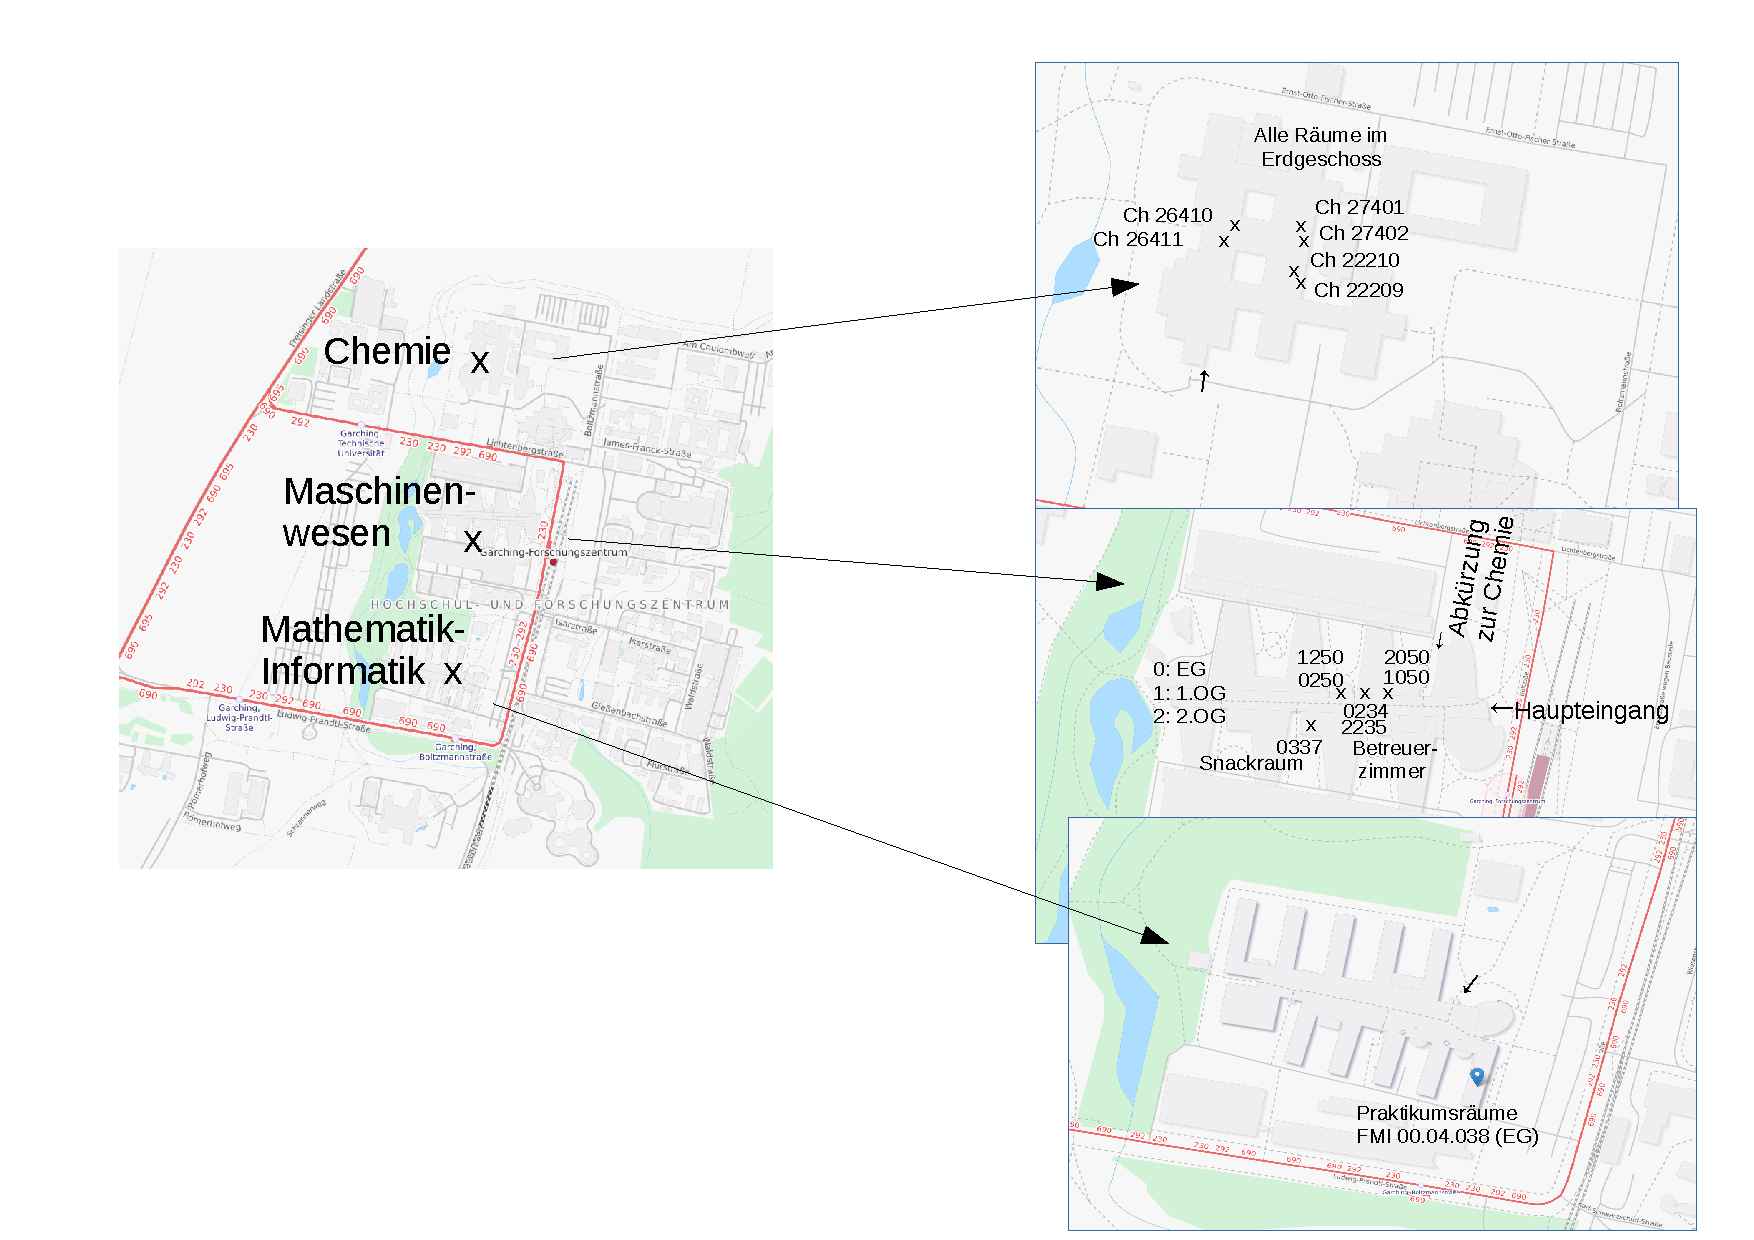
\includegraphics[scale=0.5]{campus_map.pdf}
\end{figure}
\newpage{}\begin{center}{\huge{}\textbf{Stundenplan von Dennis Rudik}}\end{center}\textbf{{\large{}Donnerstag}}\nopagebreak \\\begin{tabular} {|p{3cm} p{6cm} p{6cm}| }\hline \textbf{11:30 bis 13:45}&\textbf{Anreise zur TU München}&\textbf{Fakultät Maschinenwesen}\\\hline \textbf{12:00 bis 13:30}&\textbf{Mittagessen}&\textbf{Mensa Garching}\\\hline \textbf{14:00}&\textbf{Begrüßung}&\textbf{CH 26411}\\&Begrüßung, Besprechung des Zeitplans, Ausgabe der individuellen Stundenpläne,...&\\\hline \textbf{14:50 bis 16:20}&\textbf{Experimentieren und Auswerten}&\textbf{CH 26411}\\&Betreuer: Ann-Kathrin Raab&ca. 18 Teilnehmer\\\hline \textbf{16:40 bis 18:10}&\textbf{Einführung ins Integrieren}&\textbf{MW 1050}\\&Betreuer: Johannes Rothe&ca. 14 Teilnehmer\\\hline \textbf{18:30}&\textbf{Fahrt zur Jugendherberge}&\textbf{}\\\hline \textbf{19:00}&\textbf{Abendessen}&\textbf{Jugendherberge}\\\hline \end{tabular}\\\vspace{5.00000mm}~\\\textbf{{\large{}Freitag}}\nopagebreak \\\begin{tabular} {|p{3cm} p{6cm} p{6cm}| }\hline \textbf{06:30 bis 09:00}&\textbf{Frühstück}&\textbf{Jugendherberge}\\\hline \textbf{09:00 bis 13:00}&\textbf{Besichtigung der Forschungsneutronenquelle FRM II}&\textbf{MW 2050}\\&Betreuer: Felix Wechsler&ca. 28 Teilnehmer\\\hline \textbf{13:00 bis 14:00}&\textbf{Mittagessen}&\textbf{Mensa Garching}\\\hline \textbf{14:20 bis 15:50}&\textbf{Experiment Oszilloskop}&\textbf{Praktikum Oszilloskop}\\&Betreuer: Christopher Pfeiffer&ca. 6 Teilnehmer\\\hline \textbf{16:10 bis 17:40}&\textbf{Spezielle Relativitätstheorie}&\textbf{MW 1250}\\&Betreuer: Johannes Rothe&ca. 19 Teilnehmer\\\hline \textbf{18:00 bis 18:20}&\textbf{Erlebnisbericht IPhO}&\textbf{CH 26411}\\\hline \textbf{18:30}&\textbf{Fahrt zur Jugendherberge}&\textbf{}\\\hline \textbf{19:00}&\textbf{Abendessen}&\textbf{Jugendherberge}\\\hline \end{tabular}\\\vspace{5.00000mm}~\\\textbf{{\large{}Samstag}}\nopagebreak \\\begin{tabular} {|p{3cm} p{6cm} p{6cm}| }\hline \textbf{06:30 bis 08:00}&\textbf{Frühstück}&\textbf{Jugendherberge}\\\hline \textbf{08:00}&\textbf{Fahrt zur TU}&\textbf{}\\\hline \textbf{09:00 bis 10:30}&\textbf{Thermodynamik 2 - Statistische Physik}&\textbf{MW 1050}\\&Betreuer: Vitaly Andreev&ca. 17 Teilnehmer\\\hline \textbf{10:50 bis 12:20}&\textbf{Elektrodynamik 2}&\textbf{MW 1250}\\&Betreuer: Maximilian Keitel&ca. 21 Teilnehmer\\\hline \textbf{12:40 bis 14:00}&\textbf{Mittagessen}&\textbf{Fakultät Maschinenwesen}\\\hline \textbf{14:20 bis 15:50}&\textbf{Relativistische Teilchenphysik}&\textbf{CH 22210}\\&Betreuer: Lars Dehlwes&ca. 23 Teilnehmer\\\hline \textbf{16:10 bis 17:40}&\textbf{Quanten- und Atomphysik II}&\textbf{CH 22209}\\&Betreuer: Vitaly Andreev&ca. 28 Teilnehmer\\\hline \textbf{18:00 bis 18:20}&\textbf{Vorstellung GYPT}&\textbf{CH 26411}\\\hline \textbf{18:30}&\textbf{Fahrt zur Jugendherberge}&\textbf{}\\\hline \textbf{19:00}&\textbf{Abendessen}&\textbf{Jugendherberge}\\\hline \end{tabular}\\\vspace{5.00000mm}~\\\textbf{{\large{}Sonntag}}\nopagebreak \\\begin{tabular} {|p{3cm} p{6cm} p{6cm}| }\hline \textbf{06:30 bis 08:00}&\textbf{Frühstück}&\textbf{Jugendherberge}\\\hline \textbf{08:00}&\textbf{Fahrt zur TU}&\textbf{}\\\hline \textbf{09:00 bis 10:30}&\textbf{Theoretische Mechanik}&\textbf{CH 22210}\\&Betreuer: Eugen Dizer&ca. 13 Teilnehmer\\\hline \textbf{10:50 bis 12:20}&\textbf{Aufgabenseminar Quanten- und Atomphysik und Struktur der Materie}&\textbf{MW 1250}\\&Betreuer: Vitaly Andreev&ca. 24 Teilnehmer\\\hline \textbf{12:40 bis 13:00}&\textbf{Verabschiedung}&\textbf{CH 26411}\\\hline \textbf{13:00}&\textbf{Individuelle Abreise}&\textbf{}\\\hline \textbf{13:00 bis 14:00}&\textbf{Mittagessen}&\textbf{}\\\hline \end{tabular}\\\vspace{5.00000mm}~\\
Notfallnummern: \\
Sven Jandura: xxxx xxxxxxxxx \\
Johannes Rothe: xxxx xxxxxxxxx \\

\large Hast du Lust, die Andern vom Seminar wiederzusehen?\\
\normalsize Dann komm doch einfach zum \textbf{Vereinstreffen}. Dazu musst du kein Vereinsmitglied sein. Neben interesannten Vorträgen und Exkursionen sind jede Menge Spiel und Spaß geplant. Schau in einem Monat einfach noch mal auf der Website vorbei. Wir freuen uns, wenn du dabei bist.

\begin{figure}[!h]
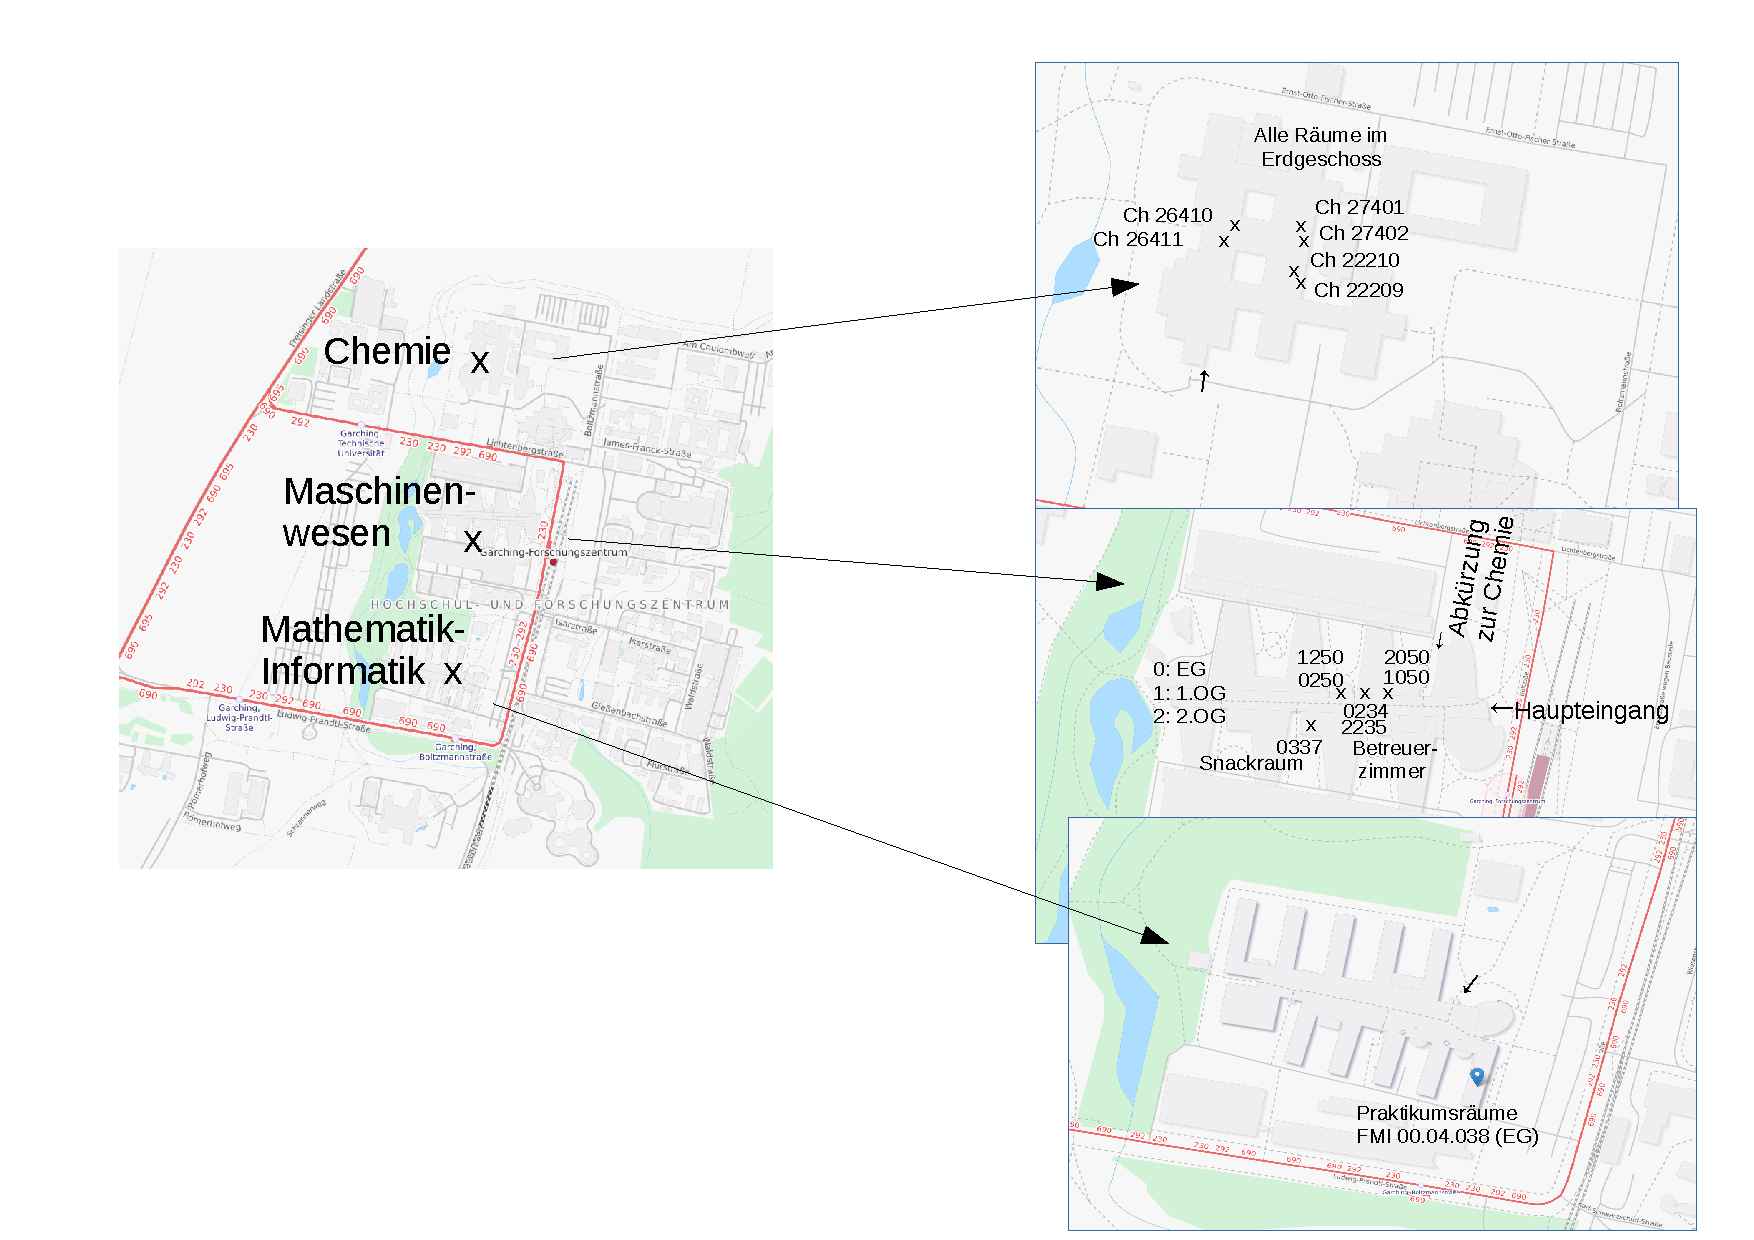
\includegraphics[scale=0.5]{campus_map.pdf}
\end{figure}
\newpage{}\begin{center}{\huge{}\textbf{Stundenplan von Eike Peters}}\end{center}\textbf{{\large{}Donnerstag}}\nopagebreak \\\begin{tabular} {|p{3cm} p{6cm} p{6cm}| }\hline \textbf{11:30 bis 13:45}&\textbf{Anreise zur TU München}&\textbf{Fakultät Maschinenwesen}\\\hline \textbf{12:00 bis 13:30}&\textbf{Mittagessen}&\textbf{Mensa Garching}\\\hline \textbf{14:00}&\textbf{Begrüßung}&\textbf{CH 26411}\\&Begrüßung, Besprechung des Zeitplans, Ausgabe der individuellen Stundenpläne,...&\\\hline \textbf{14:50 bis 16:20}&\textbf{Experimentieren und Auswerten}&\textbf{CH 26411}\\&Betreuer: Ann-Kathrin Raab&ca. 18 Teilnehmer\\\hline \textbf{16:40 bis 18:10}&\textbf{Klassische Mechanik}&\textbf{MW 1250}\\&Betreuer: Maximilian Marienhagen&ca. 10 Teilnehmer\\\hline \textbf{18:30}&\textbf{Fahrt zur Jugendherberge}&\textbf{}\\\hline \textbf{19:00}&\textbf{Abendessen}&\textbf{Jugendherberge}\\\hline \end{tabular}\\\vspace{5.00000mm}~\\\textbf{{\large{}Freitag}}\nopagebreak \\\begin{tabular} {|p{3cm} p{6cm} p{6cm}| }\hline \textbf{06:30 bis 09:00}&\textbf{Frühstück}&\textbf{Jugendherberge}\\\hline \textbf{09:00 bis 13:00}&frei&\\\hline \textbf{13:00 bis 14:00}&\textbf{Mittagessen}&\textbf{Mensa Garching}\\\hline \textbf{14:20 bis 15:50}&\textbf{Experiment Magnetismus}&\textbf{Praktikum Magnetismus}\\&Betreuer: Lars Dehlwes&ca. 6 Teilnehmer\\\hline \textbf{16:10 bis 17:40}&\textbf{Einführung ins Integrieren}&\textbf{MW 2050}\\&Betreuer: Felix Wechsler&ca. 14 Teilnehmer\\\hline \textbf{18:00 bis 18:20}&\textbf{Erlebnisbericht IPhO}&\textbf{CH 26411}\\\hline \textbf{18:30}&\textbf{Fahrt zur Jugendherberge}&\textbf{}\\\hline \textbf{19:00}&\textbf{Abendessen}&\textbf{Jugendherberge}\\\hline \end{tabular}\\\vspace{5.00000mm}~\\\textbf{{\large{}Samstag}}\nopagebreak \\\begin{tabular} {|p{3cm} p{6cm} p{6cm}| }\hline \textbf{06:30 bis 08:00}&\textbf{Frühstück}&\textbf{Jugendherberge}\\\hline \textbf{08:00}&\textbf{Fahrt zur TU}&\textbf{}\\\hline \textbf{09:00 bis 10:30}&\textbf{Aufgabenseminar klassische Mechanik}&\textbf{MW 0234}\\&Betreuer: Maximilian Marienhagen&ca. 5 Teilnehmer\\\hline \textbf{10:50 bis 12:20}&\textbf{Himmelsmechanik}&\textbf{CH 26410}\\&Betreuer: Lars Dehlwes&ca. 6 Teilnehmer\\\hline \textbf{12:40 bis 14:00}&\textbf{Mittagessen}&\textbf{Fakultät Maschinenwesen}\\\hline \textbf{14:20 bis 15:50}&\textbf{Relativistische Teilchenphysik}&\textbf{CH 22210}\\&Betreuer: Lars Dehlwes&ca. 23 Teilnehmer\\\hline \textbf{16:10 bis 17:40}&\textbf{Komplexe Wechselstromrechnung}&\textbf{MW 0250}\\&Betreuer: Vincent Grande&ca. 13 Teilnehmer\\\hline \textbf{18:00 bis 18:20}&\textbf{Vorstellung GYPT}&\textbf{CH 26411}\\\hline \textbf{18:30}&\textbf{Fahrt zur Jugendherberge}&\textbf{}\\\hline \textbf{19:00}&\textbf{Abendessen}&\textbf{Jugendherberge}\\\hline \end{tabular}\\\vspace{5.00000mm}~\\\textbf{{\large{}Sonntag}}\nopagebreak \\\begin{tabular} {|p{3cm} p{6cm} p{6cm}| }\hline \textbf{06:30 bis 08:00}&\textbf{Frühstück}&\textbf{Jugendherberge}\\\hline \textbf{08:00}&\textbf{Fahrt zur TU}&\textbf{}\\\hline \textbf{09:00 bis 10:30}&\textbf{Theoretische Mechanik}&\textbf{CH 22210}\\&Betreuer: Eugen Dizer&ca. 13 Teilnehmer\\\hline \textbf{10:50 bis 12:20}&\textbf{Elektrische Blackboxen}&\textbf{Praktikum Blackboxen}\\&Betreuer: Eugen Dizer&ca. 6 Teilnehmer\\\hline \textbf{12:40 bis 13:00}&\textbf{Verabschiedung}&\textbf{CH 26411}\\\hline \textbf{13:00}&\textbf{Individuelle Abreise}&\textbf{}\\\hline \textbf{13:00 bis 14:00}&\textbf{Mittagessen}&\textbf{}\\\hline \end{tabular}\\\vspace{5.00000mm}~\\
Notfallnummern: \\
Sven Jandura: xxxx xxxxxxxxx \\
Johannes Rothe: xxxx xxxxxxxxx \\

\large Hast du Lust, die Andern vom Seminar wiederzusehen?\\
\normalsize Dann komm doch einfach zum \textbf{Vereinstreffen}. Dazu musst du kein Vereinsmitglied sein. Neben interesannten Vorträgen und Exkursionen sind jede Menge Spiel und Spaß geplant. Schau in einem Monat einfach noch mal auf der Website vorbei. Wir freuen uns, wenn du dabei bist.

\begin{figure}[!h]
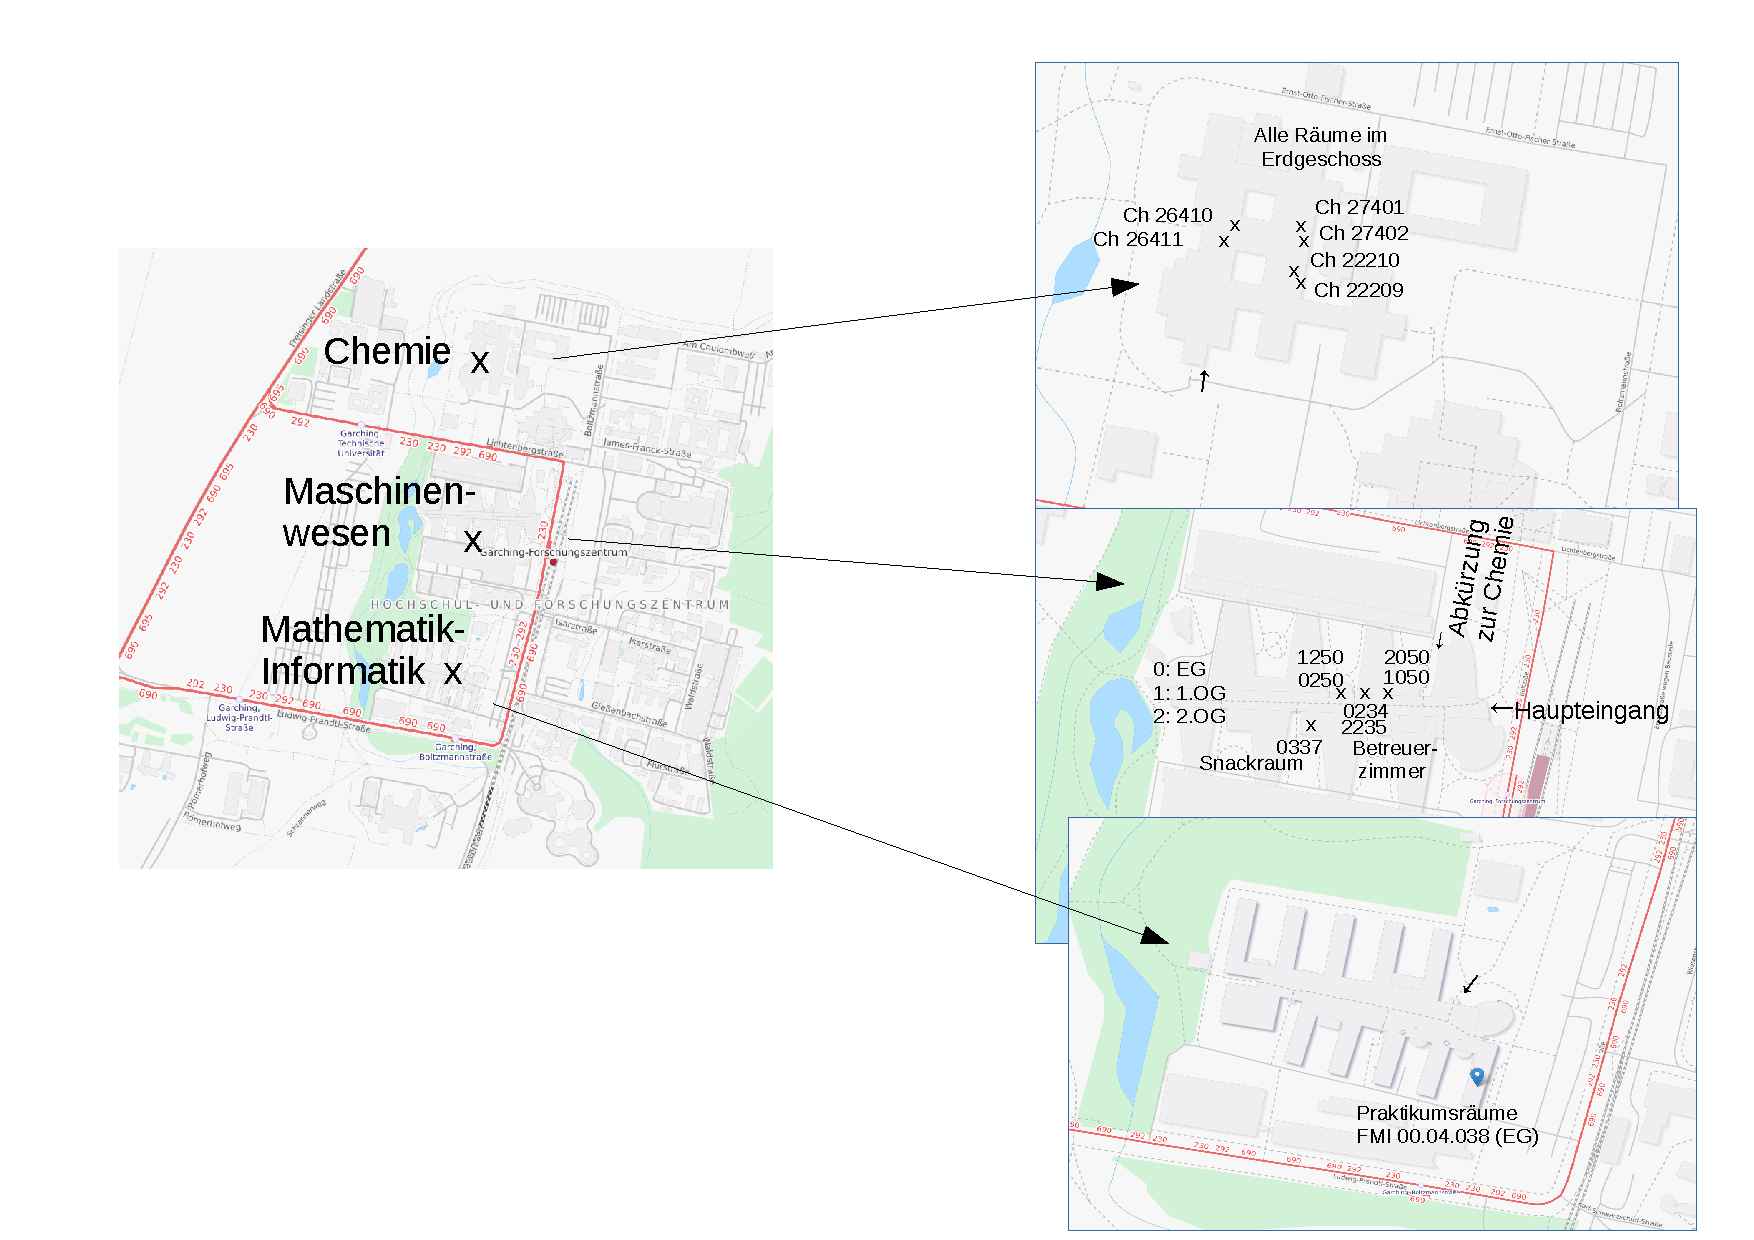
\includegraphics[scale=0.5]{campus_map.pdf}
\end{figure}
\newpage{}\begin{center}{\huge{}\textbf{Stundenplan von Elisabeth Quanz}}\end{center}\textbf{{\large{}Donnerstag}}\nopagebreak \\\begin{tabular} {|p{3cm} p{6cm} p{6cm}| }\hline \textbf{11:30 bis 13:45}&\textbf{Anreise zur TU München}&\textbf{Fakultät Maschinenwesen}\\\hline \textbf{12:00 bis 13:30}&\textbf{Mittagessen}&\textbf{Mensa Garching}\\\hline \textbf{14:00}&\textbf{Begrüßung}&\textbf{CH 26411}\\&Begrüßung, Besprechung des Zeitplans, Ausgabe der individuellen Stundenpläne,...&\\\hline \textbf{14:50 bis 16:20}&\textbf{Thermodynamik 1}&\textbf{MW 1250}\\&Betreuer: Maximilian Marienhagen&ca. 12 Teilnehmer\\\hline \textbf{16:40 bis 18:10}&\textbf{Experimentieren und Auswerten}&\textbf{CH 26411}\\&Betreuer: Ann-Kathrin Raab&ca. 15 Teilnehmer\\\hline \textbf{18:30}&\textbf{Fahrt zur Jugendherberge}&\textbf{}\\\hline \textbf{19:00}&\textbf{Abendessen}&\textbf{Jugendherberge}\\\hline \end{tabular}\\\vspace{5.00000mm}~\\\textbf{{\large{}Freitag}}\nopagebreak \\\begin{tabular} {|p{3cm} p{6cm} p{6cm}| }\hline \textbf{06:30 bis 09:00}&\textbf{Frühstück}&\textbf{Jugendherberge}\\\hline \textbf{09:00 bis 13:00}&frei&\\\hline \textbf{13:00 bis 14:00}&\textbf{Mittagessen}&\textbf{Mensa Garching}\\\hline \textbf{14:20 bis 15:50}&\textbf{Kernphysik}&\textbf{MW 0250}\\&Betreuer: Johannes Rothe&ca. 18 Teilnehmer\\\hline \textbf{16:10 bis 17:40}&\textbf{Experiment Magnetismus}&\textbf{Praktikum Magnetismus}\\&Betreuer: Lars Dehlwes&ca. 6 Teilnehmer\\\hline \textbf{18:00 bis 18:20}&\textbf{Erlebnisbericht IPhO}&\textbf{CH 26411}\\\hline \textbf{18:30}&\textbf{Fahrt zur Jugendherberge}&\textbf{}\\\hline \textbf{19:00}&\textbf{Abendessen}&\textbf{Jugendherberge}\\\hline \end{tabular}\\\vspace{5.00000mm}~\\\textbf{{\large{}Samstag}}\nopagebreak \\\begin{tabular} {|p{3cm} p{6cm} p{6cm}| }\hline \textbf{06:30 bis 08:00}&\textbf{Frühstück}&\textbf{Jugendherberge}\\\hline \textbf{08:00}&\textbf{Fahrt zur TU}&\textbf{}\\\hline \textbf{09:00 bis 10:30}&\textbf{Experiment Millikan-Versuch}&\textbf{Praktikum Millikan-Versuch}\\&Betreuer: Samuel Moll&ca. 6 Teilnehmer\\\hline \textbf{10:50 bis 12:20}&\textbf{Spezielle Relativitätstheorie}&\textbf{MW 0250}\\&Betreuer: Johannes Rothe&ca. 12 Teilnehmer\\\hline \textbf{12:40 bis 14:00}&\textbf{Mittagessen}&\textbf{Fakultät Maschinenwesen}\\\hline \textbf{14:20 bis 15:50}&\textbf{Rotationsbewegungen}&\textbf{MW 0250}\\&Betreuer: Vincent Grande&ca. 3 Teilnehmer\\\hline \textbf{16:10 bis 17:40}&\textbf{Aufgabenseminar klassische Mechanik}&\textbf{MW 2050}\\&Betreuer: Aaron Wild&ca. 5 Teilnehmer\\\hline \textbf{18:00 bis 18:20}&\textbf{Vorstellung GYPT}&\textbf{CH 26411}\\\hline \textbf{18:30}&\textbf{Fahrt zur Jugendherberge}&\textbf{}\\\hline \textbf{19:00}&\textbf{Abendessen}&\textbf{Jugendherberge}\\\hline \end{tabular}\\\vspace{5.00000mm}~\\\textbf{{\large{}Sonntag}}\nopagebreak \\\begin{tabular} {|p{3cm} p{6cm} p{6cm}| }\hline \textbf{06:30 bis 08:00}&\textbf{Frühstück}&\textbf{Jugendherberge}\\\hline \textbf{08:00}&\textbf{Fahrt zur TU}&\textbf{}\\\hline \textbf{09:00 bis 10:30}&\textbf{Aufgabenseminar Wärmelehre}&\textbf{CH 22209}\\&Betreuer: Maximilian Marienhagen&ca. 9 Teilnehmer\\\hline \textbf{10:50 bis 12:20}&\textbf{Bestimmung des Brechungskoeffizienten von Plexiglas}&\textbf{MW 0234}\\&Betreuer: Lilith Diringer&ca. 8 Teilnehmer\\\hline \textbf{12:40 bis 13:00}&\textbf{Verabschiedung}&\textbf{CH 26411}\\\hline \textbf{13:00}&\textbf{Individuelle Abreise}&\textbf{}\\\hline \textbf{13:00 bis 14:00}&\textbf{Mittagessen}&\textbf{}\\\hline \end{tabular}\\\vspace{5.00000mm}~\\
Notfallnummern: \\
Sven Jandura: xxxx xxxxxxxxx \\
Johannes Rothe: xxxx xxxxxxxxx \\

\large Hast du Lust, die Andern vom Seminar wiederzusehen?\\
\normalsize Dann komm doch einfach zum \textbf{Vereinstreffen}. Dazu musst du kein Vereinsmitglied sein. Neben interesannten Vorträgen und Exkursionen sind jede Menge Spiel und Spaß geplant. Schau in einem Monat einfach noch mal auf der Website vorbei. Wir freuen uns, wenn du dabei bist.

\begin{figure}[!h]
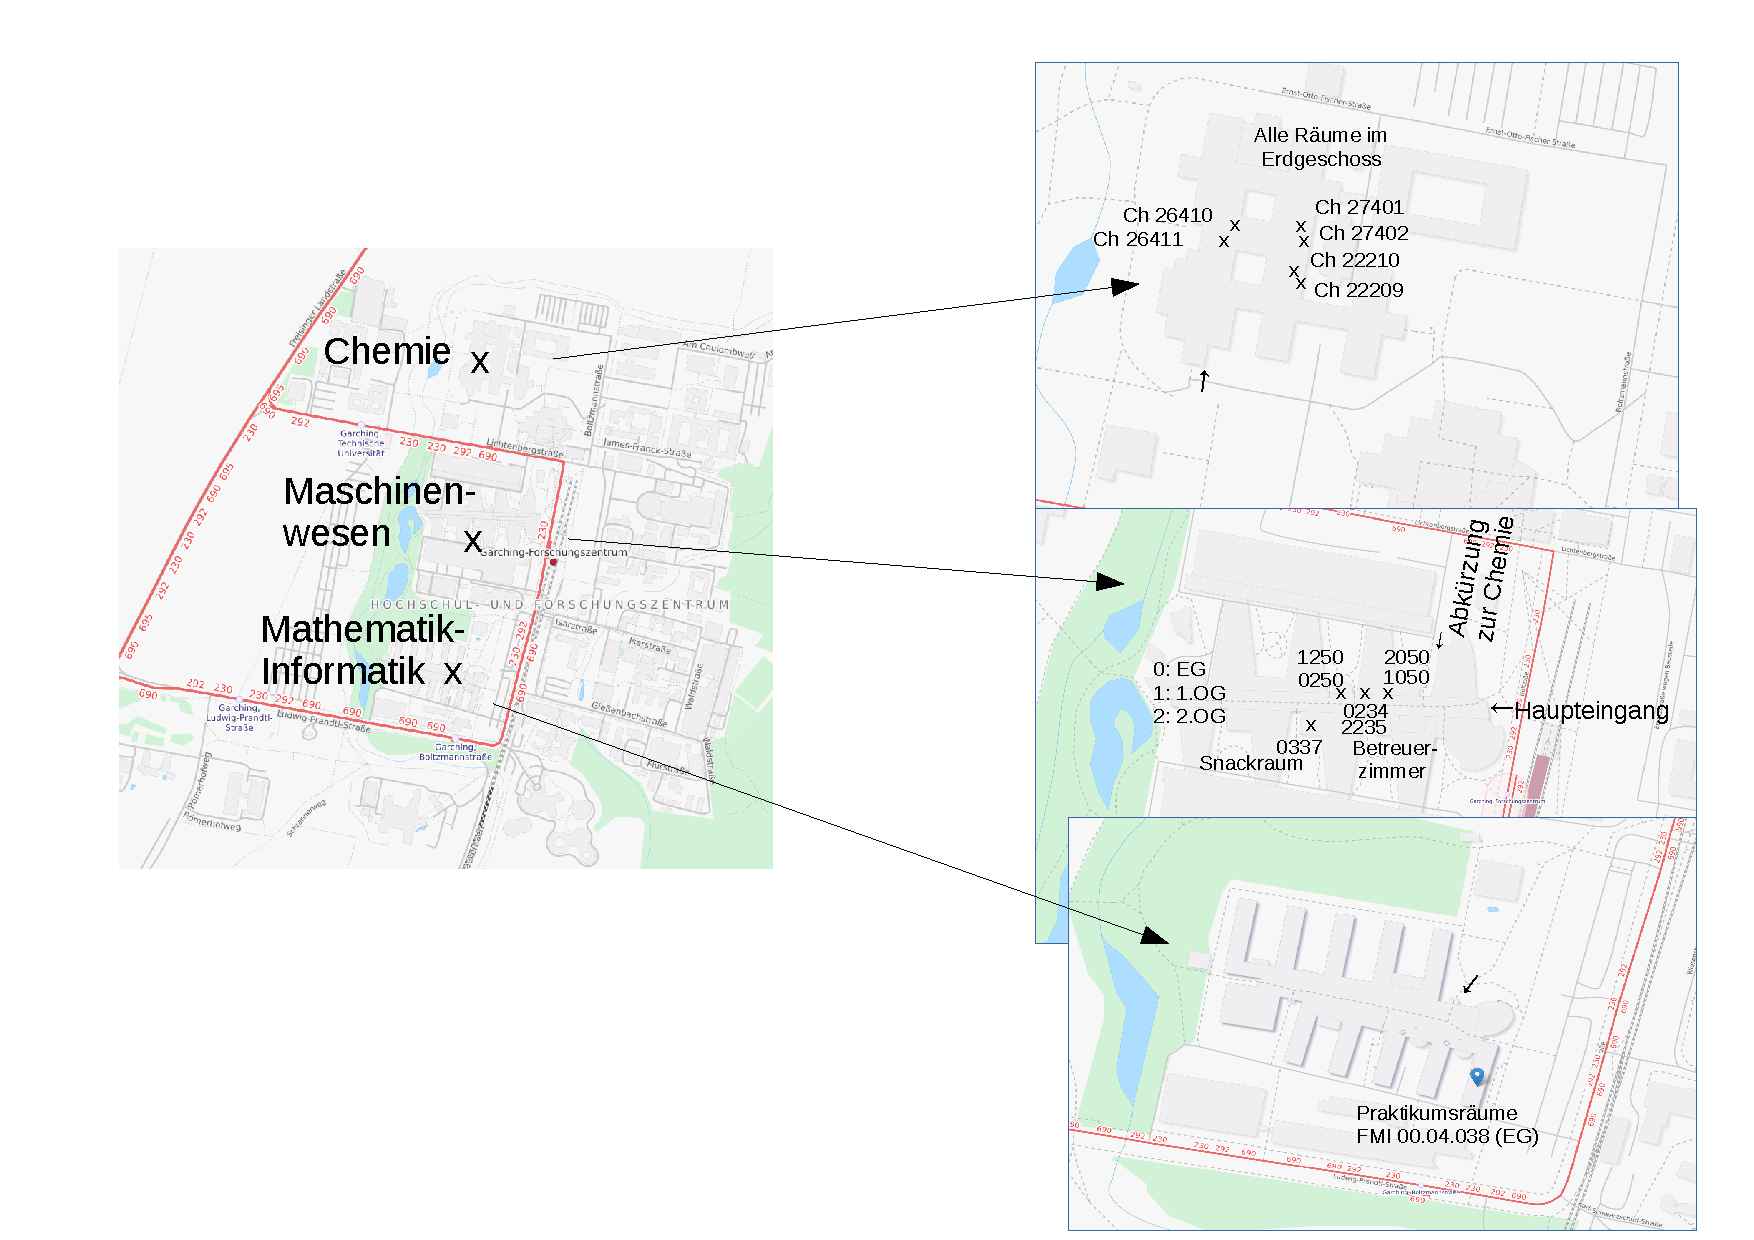
\includegraphics[scale=0.5]{campus_map.pdf}
\end{figure}
\newpage{}\begin{center}{\huge{}\textbf{Stundenplan von Ella Hutschenreiter}}\end{center}\textbf{{\large{}Donnerstag}}\nopagebreak \\\begin{tabular} {|p{3cm} p{6cm} p{6cm}| }\hline \textbf{11:30 bis 13:45}&\textbf{Anreise zur TU München}&\textbf{Fakultät Maschinenwesen}\\\hline \textbf{12:00 bis 13:30}&\textbf{Mittagessen}&\textbf{Mensa Garching}\\\hline \textbf{14:00}&\textbf{Begrüßung}&\textbf{CH 26411}\\&Begrüßung, Besprechung des Zeitplans, Ausgabe der individuellen Stundenpläne,...&\\\hline \textbf{14:50 bis 16:20}&\textbf{Einführung ins Differenzieren}&\textbf{MW 1050}\\&Betreuer: Ilja Göthel&ca. 6 Teilnehmer\\\hline \textbf{16:40 bis 18:10}&\textbf{Näherungsmethoden}&\textbf{MW 0234}\\&Betreuer: Ilja Göthel&ca. 13 Teilnehmer\\\hline \textbf{18:30}&\textbf{Fahrt zur Jugendherberge}&\textbf{}\\\hline \textbf{19:00}&\textbf{Abendessen}&\textbf{Jugendherberge}\\\hline \end{tabular}\\\vspace{5.00000mm}~\\\textbf{{\large{}Freitag}}\nopagebreak \\\begin{tabular} {|p{3cm} p{6cm} p{6cm}| }\hline \textbf{06:30 bis 09:00}&\textbf{Frühstück}&\textbf{Jugendherberge}\\\hline \textbf{09:00 bis 13:00}&\textbf{Besichtigung der Forschungsneutronenquelle FRM II}&\textbf{MW 2050}\\&Betreuer: Felix Wechsler&ca. 28 Teilnehmer\\\hline \textbf{13:00 bis 14:00}&\textbf{Mittagessen}&\textbf{Mensa Garching}\\\hline \textbf{14:20 bis 15:50}&\textbf{Experiment spezifische Elektronenladung}&\textbf{Praktikum spezifische Elektronenladung}\\&Betreuer: Felix Wechsler&ca. 6 Teilnehmer\\\hline \textbf{16:10 bis 17:40}&\textbf{Einführung ins Integrieren}&\textbf{MW 2050}\\&Betreuer: Felix Wechsler&ca. 14 Teilnehmer\\\hline \textbf{18:00 bis 18:20}&\textbf{Erlebnisbericht IPhO}&\textbf{CH 26411}\\\hline \textbf{18:30}&\textbf{Fahrt zur Jugendherberge}&\textbf{}\\\hline \textbf{19:00}&\textbf{Abendessen}&\textbf{Jugendherberge}\\\hline \end{tabular}\\\vspace{5.00000mm}~\\\textbf{{\large{}Samstag}}\nopagebreak \\\begin{tabular} {|p{3cm} p{6cm} p{6cm}| }\hline \textbf{06:30 bis 08:00}&\textbf{Frühstück}&\textbf{Jugendherberge}\\\hline \textbf{08:00}&\textbf{Fahrt zur TU}&\textbf{}\\\hline \textbf{09:00 bis 10:30}&\textbf{Thermodynamik 2 - Statistische Physik}&\textbf{MW 1050}\\&Betreuer: Vitaly Andreev&ca. 17 Teilnehmer\\\hline \textbf{10:50 bis 12:20}&\textbf{Experiment Reversionspendel}&\textbf{Praktikum Reversionspendel}\\&Betreuer: Lilith Diringer&ca. 6 Teilnehmer\\\hline \textbf{12:40 bis 14:00}&\textbf{Mittagessen}&\textbf{Fakultät Maschinenwesen}\\\hline \textbf{14:20 bis 15:50}&\textbf{Thermodynamik 1}&\textbf{MW 1250}\\&Betreuer: Maximilian Marienhagen&ca. 9 Teilnehmer\\\hline \textbf{16:10 bis 17:40}&\textbf{Aufgabenseminar klassische Mechanik}&\textbf{MW 2050}\\&Betreuer: Aaron Wild&ca. 5 Teilnehmer\\\hline \textbf{18:00 bis 18:20}&\textbf{Vorstellung GYPT}&\textbf{CH 26411}\\\hline \textbf{18:30}&\textbf{Fahrt zur Jugendherberge}&\textbf{}\\\hline \textbf{19:00}&\textbf{Abendessen}&\textbf{Jugendherberge}\\\hline \end{tabular}\\\vspace{5.00000mm}~\\\textbf{{\large{}Sonntag}}\nopagebreak \\\begin{tabular} {|p{3cm} p{6cm} p{6cm}| }\hline \textbf{06:30 bis 08:00}&\textbf{Frühstück}&\textbf{Jugendherberge}\\\hline \textbf{08:00}&\textbf{Fahrt zur TU}&\textbf{}\\\hline \textbf{09:00 bis 10:30}&\textbf{Wellenoptik}&\textbf{MW 2050}\\&Betreuer: Christopher Pfeiffer&ca. 14 Teilnehmer\\\hline \textbf{10:50 bis 12:20}&\textbf{Rotationsbewegungen}&\textbf{CH 26410}\\&Betreuer: Vincent Grande&ca. 9 Teilnehmer\\\hline \textbf{12:40 bis 13:00}&\textbf{Verabschiedung}&\textbf{CH 26411}\\\hline \textbf{13:00}&\textbf{Individuelle Abreise}&\textbf{}\\\hline \textbf{13:00 bis 14:00}&\textbf{Mittagessen}&\textbf{}\\\hline \end{tabular}\\\vspace{5.00000mm}~\\
Notfallnummern: \\
Sven Jandura: xxxx xxxxxxxxx \\
Johannes Rothe: xxxx xxxxxxxxx \\

\large Hast du Lust, die Andern vom Seminar wiederzusehen?\\
\normalsize Dann komm doch einfach zum \textbf{Vereinstreffen}. Dazu musst du kein Vereinsmitglied sein. Neben interesannten Vorträgen und Exkursionen sind jede Menge Spiel und Spaß geplant. Schau in einem Monat einfach noch mal auf der Website vorbei. Wir freuen uns, wenn du dabei bist.

\begin{figure}[!h]
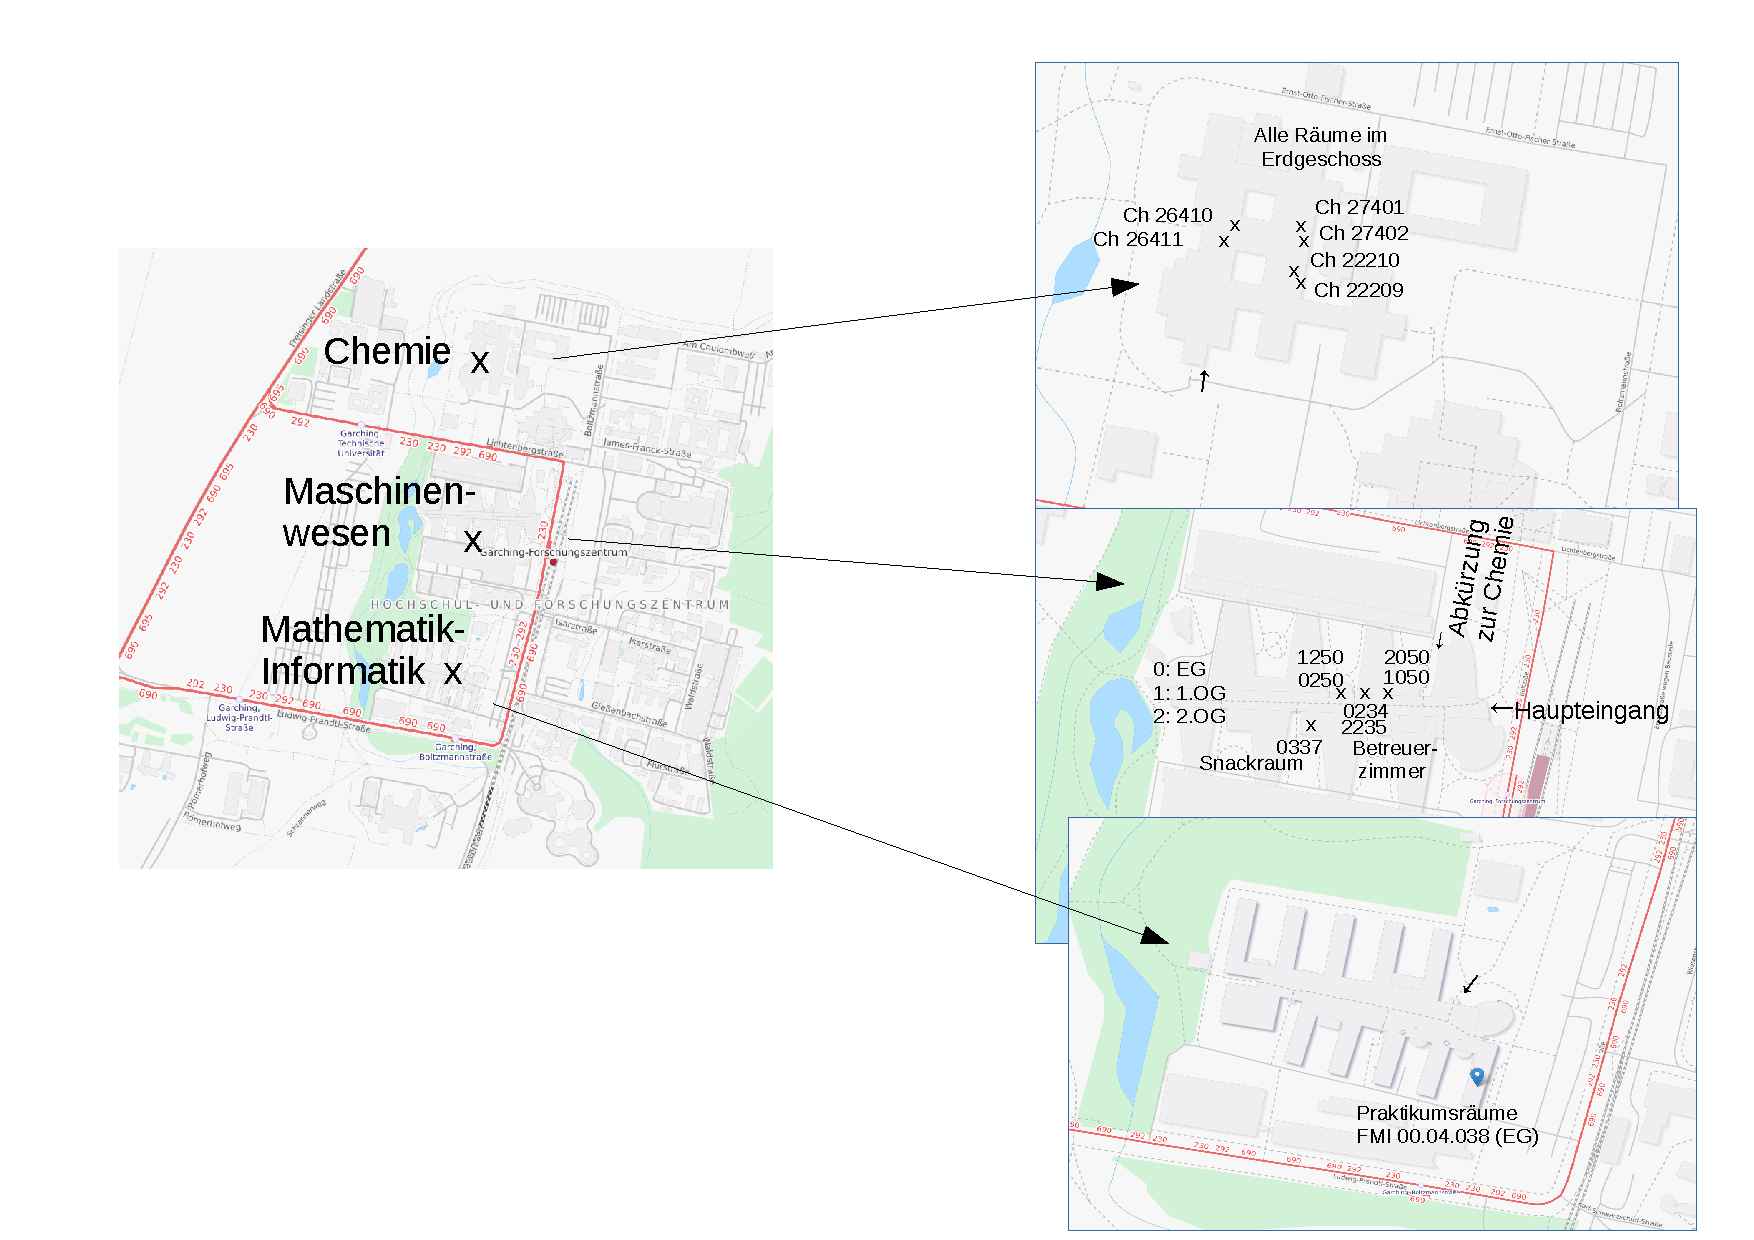
\includegraphics[scale=0.5]{campus_map.pdf}
\end{figure}
\newpage{}\begin{center}{\huge{}\textbf{Stundenplan von Erik Sünderhauf}}\end{center}\textbf{{\large{}Donnerstag}}\nopagebreak \\\begin{tabular} {|p{3cm} p{6cm} p{6cm}| }\hline \textbf{11:30 bis 13:45}&\textbf{Anreise zur TU München}&\textbf{Fakultät Maschinenwesen}\\\hline \textbf{12:00 bis 13:30}&\textbf{Mittagessen}&\textbf{Mensa Garching}\\\hline \textbf{14:00}&\textbf{Begrüßung}&\textbf{CH 26411}\\&Begrüßung, Besprechung des Zeitplans, Ausgabe der individuellen Stundenpläne,...&\\\hline \textbf{14:50 bis 16:20}&\textbf{Experimentieren und Auswerten}&\textbf{CH 26411}\\&Betreuer: Ann-Kathrin Raab&ca. 18 Teilnehmer\\\hline \textbf{16:40 bis 18:10}&\textbf{Himmelsmechanik}&\textbf{MW 2050}\\&Betreuer: Lars Dehlwes&ca. 19 Teilnehmer\\\hline \textbf{18:30}&\textbf{Fahrt zur Jugendherberge}&\textbf{}\\\hline \textbf{19:00}&\textbf{Abendessen}&\textbf{Jugendherberge}\\\hline \end{tabular}\\\vspace{5.00000mm}~\\\textbf{{\large{}Freitag}}\nopagebreak \\\begin{tabular} {|p{3cm} p{6cm} p{6cm}| }\hline \textbf{06:30 bis 09:00}&\textbf{Frühstück}&\textbf{Jugendherberge}\\\hline \textbf{09:00 bis 13:00}&\textbf{Besichtigung der Forschungsneutronenquelle FRM II}&\textbf{MW 2050}\\&Betreuer: Felix Wechsler&ca. 28 Teilnehmer\\\hline \textbf{13:00 bis 14:00}&\textbf{Mittagessen}&\textbf{Mensa Garching}\\\hline \textbf{14:20 bis 15:50}&\textbf{Experiment Magnetismus}&\textbf{Praktikum Magnetismus}\\&Betreuer: Lars Dehlwes&ca. 6 Teilnehmer\\\hline \textbf{16:10 bis 17:40}&\textbf{Näherungsmethoden}&\textbf{CH 26410}\\&Betreuer: Vincent Grande&ca. 11 Teilnehmer\\\hline \textbf{18:00 bis 18:20}&\textbf{Erlebnisbericht IPhO}&\textbf{CH 26411}\\\hline \textbf{18:30}&\textbf{Fahrt zur Jugendherberge}&\textbf{}\\\hline \textbf{19:00}&\textbf{Abendessen}&\textbf{Jugendherberge}\\\hline \end{tabular}\\\vspace{5.00000mm}~\\\textbf{{\large{}Samstag}}\nopagebreak \\\begin{tabular} {|p{3cm} p{6cm} p{6cm}| }\hline \textbf{06:30 bis 08:00}&\textbf{Frühstück}&\textbf{Jugendherberge}\\\hline \textbf{08:00}&\textbf{Fahrt zur TU}&\textbf{}\\\hline \textbf{09:00 bis 10:30}&\textbf{Elektrodynamik 1}&\textbf{MW 1250}\\&Betreuer: Maximilian Keitel&ca. 21 Teilnehmer\\\hline \textbf{10:50 bis 12:20}&\textbf{Spezielle Relativitätstheorie}&\textbf{MW 0250}\\&Betreuer: Johannes Rothe&ca. 12 Teilnehmer\\\hline \textbf{12:40 bis 14:00}&\textbf{Mittagessen}&\textbf{Fakultät Maschinenwesen}\\\hline \textbf{14:20 bis 15:50}&\textbf{Relativistische Teilchenphysik}&\textbf{CH 22210}\\&Betreuer: Lars Dehlwes&ca. 23 Teilnehmer\\\hline \textbf{16:10 bis 17:40}&\textbf{Aufgabenseminar Elektrodynamik}&\textbf{MW 1250}\\&Betreuer: Maximilian Keitel&ca. 8 Teilnehmer\\\hline \textbf{18:00 bis 18:20}&\textbf{Vorstellung GYPT}&\textbf{CH 26411}\\\hline \textbf{18:30}&\textbf{Fahrt zur Jugendherberge}&\textbf{}\\\hline \textbf{19:00}&\textbf{Abendessen}&\textbf{Jugendherberge}\\\hline \end{tabular}\\\vspace{5.00000mm}~\\\textbf{{\large{}Sonntag}}\nopagebreak \\\begin{tabular} {|p{3cm} p{6cm} p{6cm}| }\hline \textbf{06:30 bis 08:00}&\textbf{Frühstück}&\textbf{Jugendherberge}\\\hline \textbf{08:00}&\textbf{Fahrt zur TU}&\textbf{}\\\hline \textbf{09:00 bis 10:30}&\textbf{Theoretische Mechanik}&\textbf{CH 22210}\\&Betreuer: Eugen Dizer&ca. 13 Teilnehmer\\\hline \textbf{10:50 bis 12:20}&\textbf{Aufgabenseminar klassische Mechanik}&\textbf{CH 22209}\\&Betreuer: Aaron Wild&ca. 11 Teilnehmer\\\hline \textbf{12:40 bis 13:00}&\textbf{Verabschiedung}&\textbf{CH 26411}\\\hline \textbf{13:00}&\textbf{Individuelle Abreise}&\textbf{}\\\hline \textbf{13:00 bis 14:00}&\textbf{Mittagessen}&\textbf{}\\\hline \end{tabular}\\\vspace{5.00000mm}~\\
Notfallnummern: \\
Sven Jandura: xxxx xxxxxxxxx \\
Johannes Rothe: xxxx xxxxxxxxx \\

\large Hast du Lust, die Andern vom Seminar wiederzusehen?\\
\normalsize Dann komm doch einfach zum \textbf{Vereinstreffen}. Dazu musst du kein Vereinsmitglied sein. Neben interesannten Vorträgen und Exkursionen sind jede Menge Spiel und Spaß geplant. Schau in einem Monat einfach noch mal auf der Website vorbei. Wir freuen uns, wenn du dabei bist.

\begin{figure}[!h]
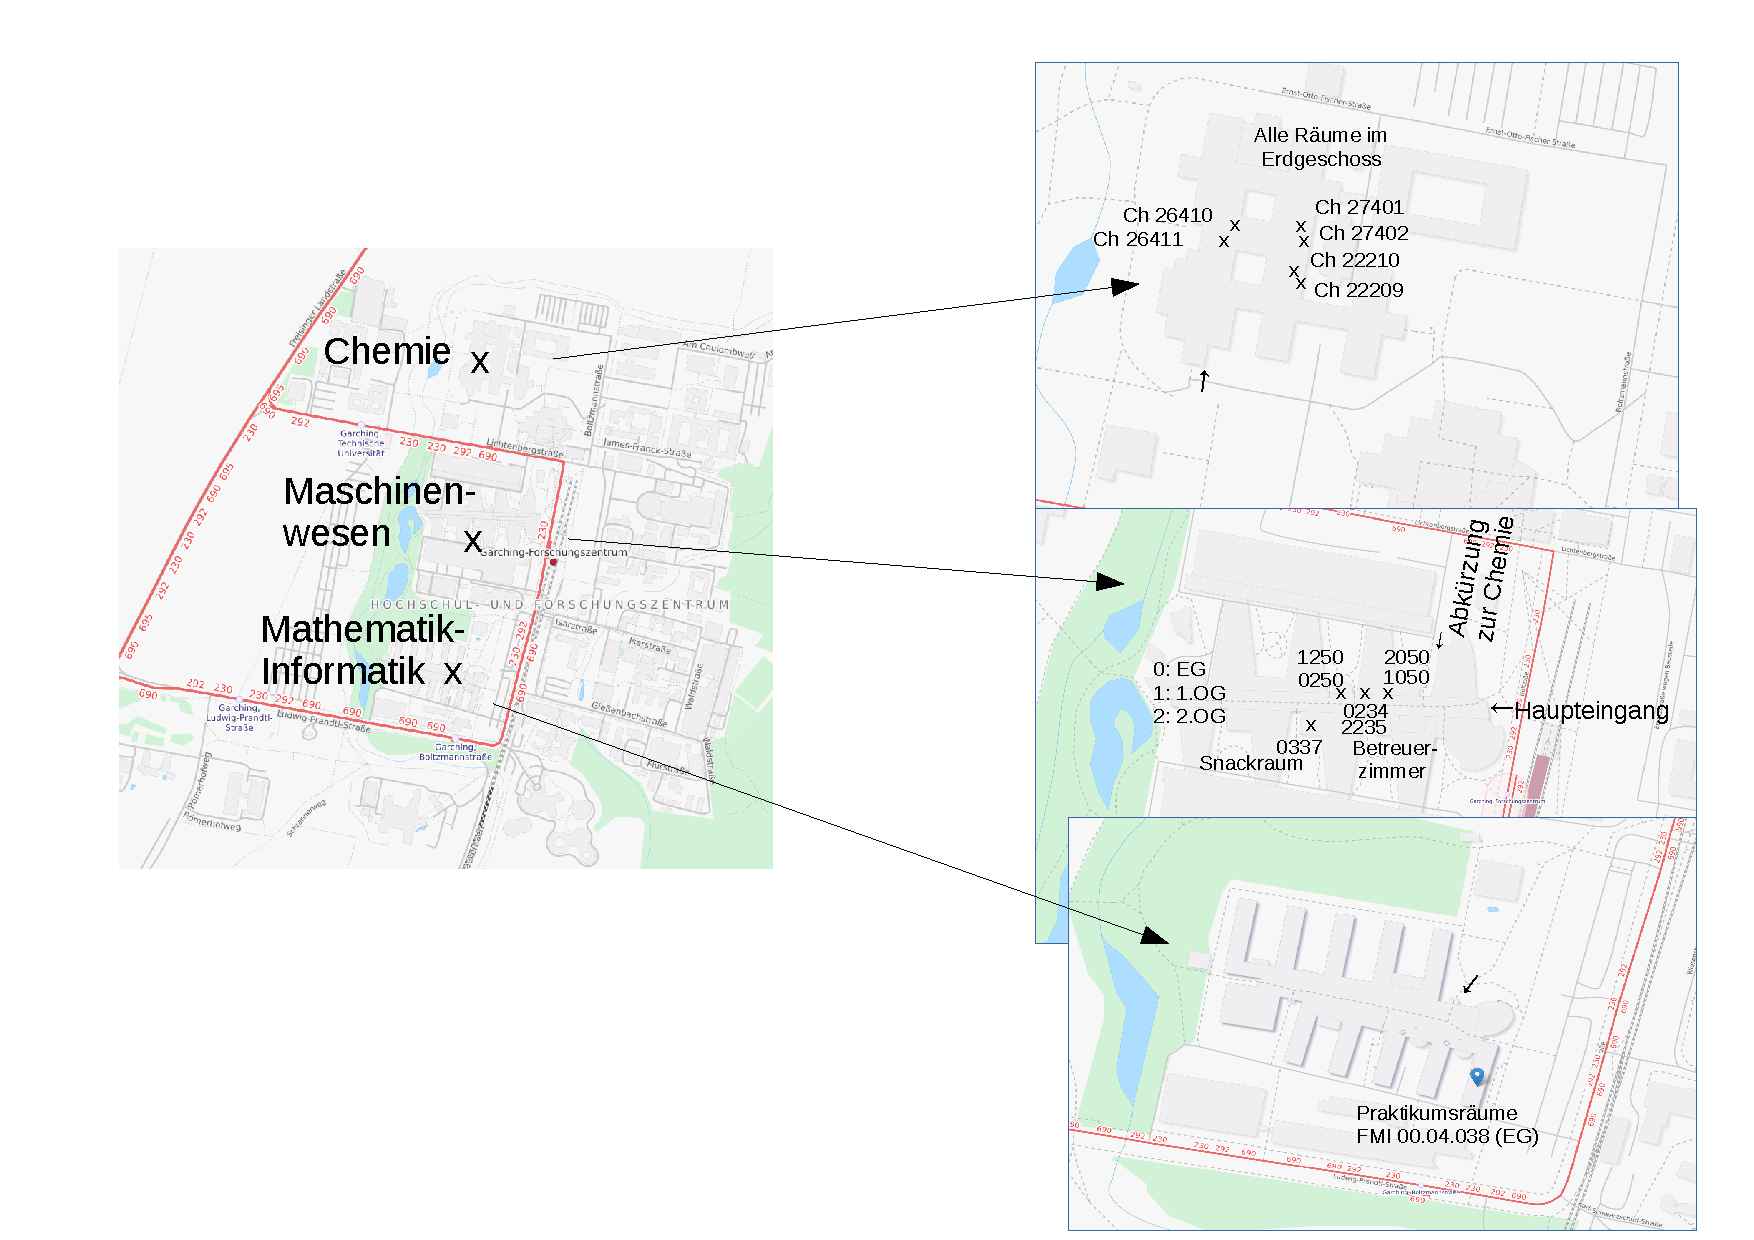
\includegraphics[scale=0.5]{campus_map.pdf}
\end{figure}
\newpage{}\begin{center}{\huge{}\textbf{Stundenplan von Fabian Henn}}\end{center}\textbf{{\large{}Donnerstag}}\nopagebreak \\\begin{tabular} {|p{3cm} p{6cm} p{6cm}| }\hline \textbf{11:30 bis 13:45}&\textbf{Anreise zur TU München}&\textbf{Fakultät Maschinenwesen}\\\hline \textbf{12:00 bis 13:30}&\textbf{Mittagessen}&\textbf{Mensa Garching}\\\hline \textbf{14:00}&\textbf{Begrüßung}&\textbf{CH 26411}\\&Begrüßung, Besprechung des Zeitplans, Ausgabe der individuellen Stundenpläne,...&\\\hline \textbf{14:50 bis 16:20}&\textbf{Experimentieren und Auswerten}&\textbf{CH 26411}\\&Betreuer: Ann-Kathrin Raab&ca. 18 Teilnehmer\\\hline \textbf{16:40 bis 18:10}&\textbf{Näherungsmethoden}&\textbf{MW 0234}\\&Betreuer: Ilja Göthel&ca. 13 Teilnehmer\\\hline \textbf{18:30}&\textbf{Fahrt zur Jugendherberge}&\textbf{}\\\hline \textbf{19:00}&\textbf{Abendessen}&\textbf{Jugendherberge}\\\hline \end{tabular}\\\vspace{5.00000mm}~\\\textbf{{\large{}Freitag}}\nopagebreak \\\begin{tabular} {|p{3cm} p{6cm} p{6cm}| }\hline \textbf{06:30 bis 09:00}&\textbf{Frühstück}&\textbf{Jugendherberge}\\\hline \textbf{09:00 bis 13:00}&frei&\\\hline \textbf{13:00 bis 14:00}&\textbf{Mittagessen}&\textbf{Mensa Garching}\\\hline \textbf{14:20 bis 15:50}&\textbf{Rotationsbewegungen}&\textbf{MW 1050}\\&Betreuer: Vincent Grande&ca. 6 Teilnehmer\\\hline \textbf{16:10 bis 17:40}&\textbf{Einführung ins Integrieren}&\textbf{MW 2050}\\&Betreuer: Felix Wechsler&ca. 14 Teilnehmer\\\hline \textbf{18:00 bis 18:20}&\textbf{Erlebnisbericht IPhO}&\textbf{CH 26411}\\\hline \textbf{18:30}&\textbf{Fahrt zur Jugendherberge}&\textbf{}\\\hline \textbf{19:00}&\textbf{Abendessen}&\textbf{Jugendherberge}\\\hline \end{tabular}\\\vspace{5.00000mm}~\\\textbf{{\large{}Samstag}}\nopagebreak \\\begin{tabular} {|p{3cm} p{6cm} p{6cm}| }\hline \textbf{06:30 bis 08:00}&\textbf{Frühstück}&\textbf{Jugendherberge}\\\hline \textbf{08:00}&\textbf{Fahrt zur TU}&\textbf{}\\\hline \textbf{09:00 bis 10:30}&\textbf{Thermodynamik 2 - Statistische Physik}&\textbf{MW 1050}\\&Betreuer: Vitaly Andreev&ca. 17 Teilnehmer\\\hline \textbf{10:50 bis 12:20}&\textbf{Elektrodynamik 2}&\textbf{MW 1250}\\&Betreuer: Maximilian Keitel&ca. 21 Teilnehmer\\\hline \textbf{12:40 bis 14:00}&\textbf{Mittagessen}&\textbf{Fakultät Maschinenwesen}\\\hline \textbf{14:20 bis 15:50}&\textbf{Quanten- und Atomphysik I}&\textbf{CH 22209}\\&Betreuer: Vitaly Andreev&ca. 22 Teilnehmer\\\hline \textbf{16:10 bis 17:40}&\textbf{Quanten- und Atomphysik II}&\textbf{CH 22209}\\&Betreuer: Vitaly Andreev&ca. 28 Teilnehmer\\\hline \textbf{18:00 bis 18:20}&\textbf{Vorstellung GYPT}&\textbf{CH 26411}\\\hline \textbf{18:30}&\textbf{Fahrt zur Jugendherberge}&\textbf{}\\\hline \textbf{19:00}&\textbf{Abendessen}&\textbf{Jugendherberge}\\\hline \end{tabular}\\\vspace{5.00000mm}~\\\textbf{{\large{}Sonntag}}\nopagebreak \\\begin{tabular} {|p{3cm} p{6cm} p{6cm}| }\hline \textbf{06:30 bis 08:00}&\textbf{Frühstück}&\textbf{Jugendherberge}\\\hline \textbf{08:00}&\textbf{Fahrt zur TU}&\textbf{}\\\hline \textbf{09:00 bis 10:30}&\textbf{Wellenoptik}&\textbf{MW 2050}\\&Betreuer: Christopher Pfeiffer&ca. 14 Teilnehmer\\\hline \textbf{10:50 bis 12:20}&\textbf{Relativistische Teilchenphysik}&\textbf{CH 22210}\\&Betreuer: Lars Dehlwes&ca. 11 Teilnehmer\\\hline \textbf{12:40 bis 13:00}&\textbf{Verabschiedung}&\textbf{CH 26411}\\\hline \textbf{13:00}&\textbf{Individuelle Abreise}&\textbf{}\\\hline \textbf{13:00 bis 14:00}&\textbf{Mittagessen}&\textbf{}\\\hline \end{tabular}\\\vspace{5.00000mm}~\\
Notfallnummern: \\
Sven Jandura: xxxx xxxxxxxxx \\
Johannes Rothe: xxxx xxxxxxxxx \\

\large Hast du Lust, die Andern vom Seminar wiederzusehen?\\
\normalsize Dann komm doch einfach zum \textbf{Vereinstreffen}. Dazu musst du kein Vereinsmitglied sein. Neben interesannten Vorträgen und Exkursionen sind jede Menge Spiel und Spaß geplant. Schau in einem Monat einfach noch mal auf der Website vorbei. Wir freuen uns, wenn du dabei bist.

\begin{figure}[!h]
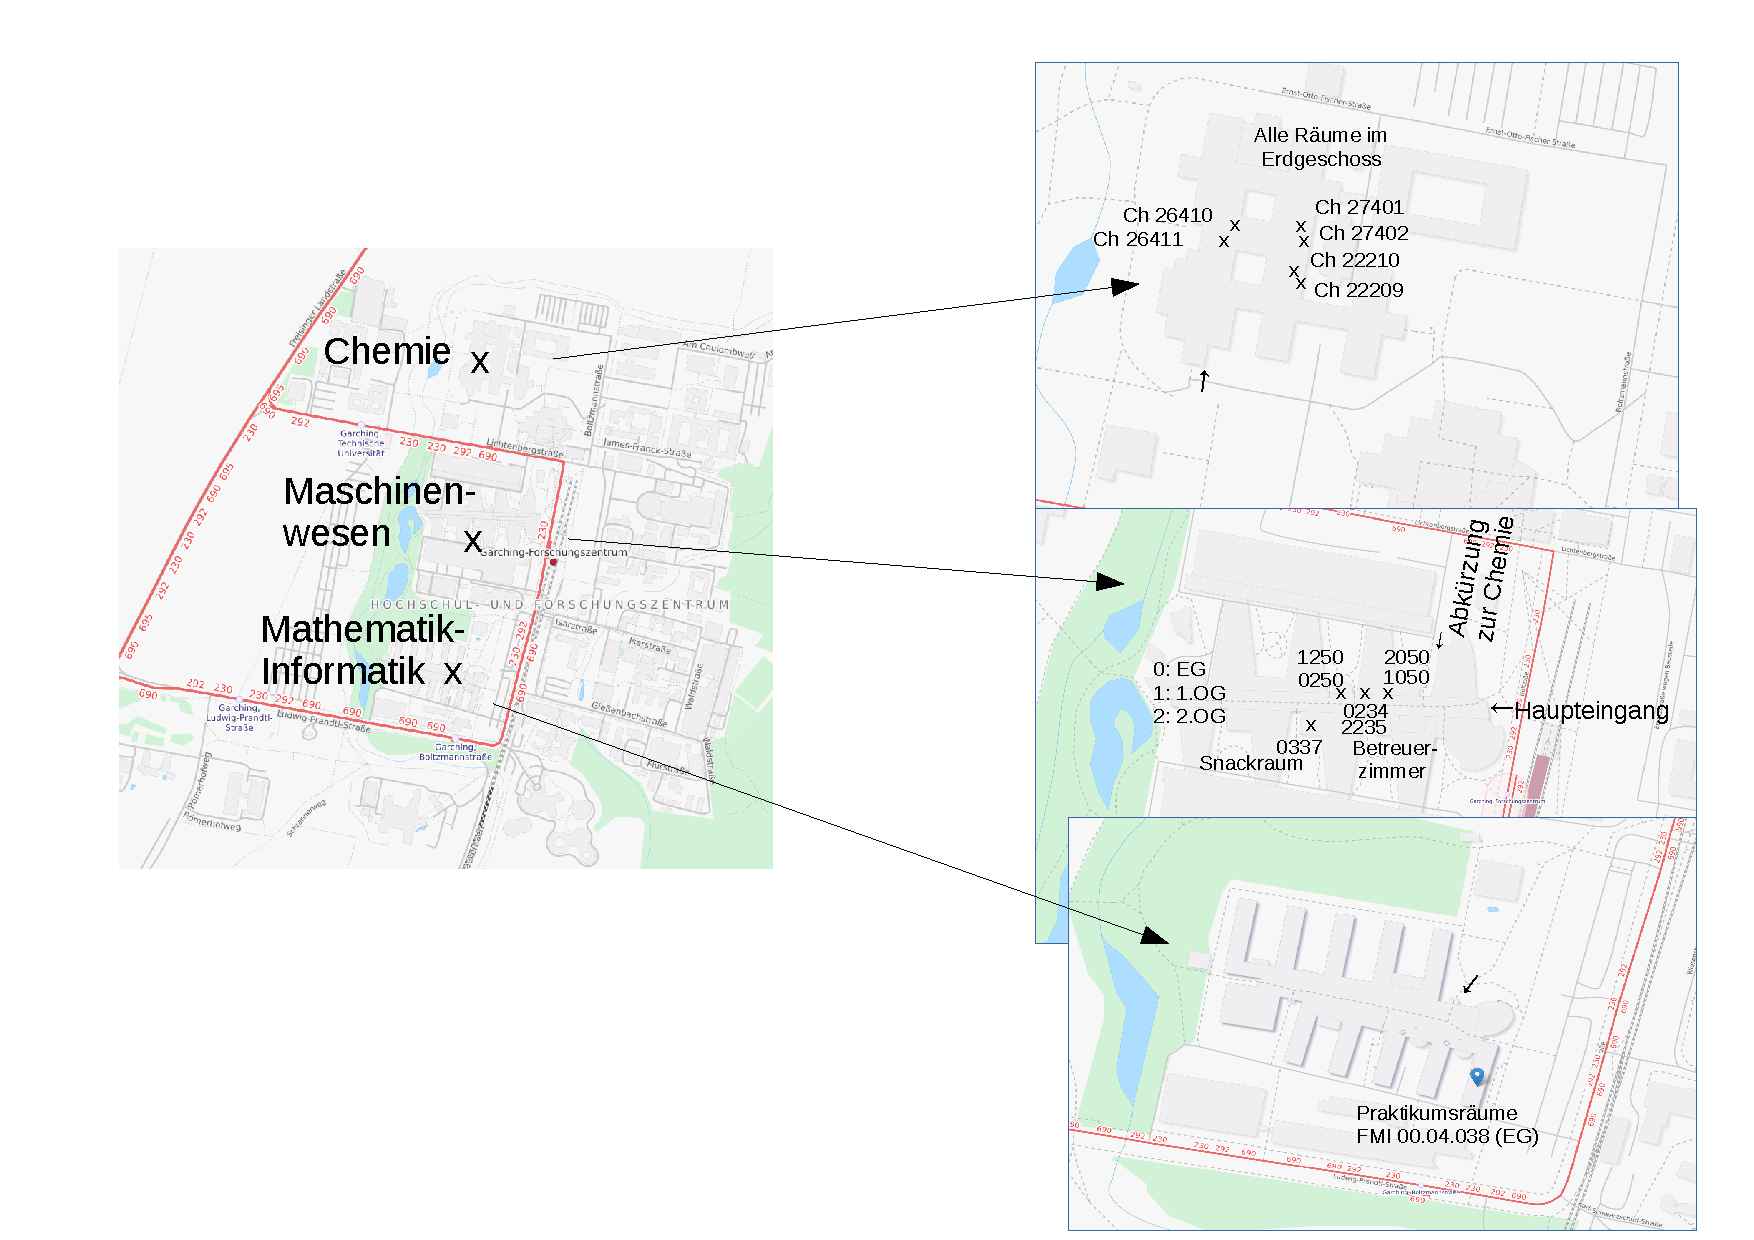
\includegraphics[scale=0.5]{campus_map.pdf}
\end{figure}
\newpage{}\begin{center}{\huge{}\textbf{Stundenplan von Felix Vogel}}\end{center}\textbf{{\large{}Donnerstag}}\nopagebreak \\\begin{tabular} {|p{3cm} p{6cm} p{6cm}| }\hline \textbf{11:30 bis 13:45}&\textbf{Anreise zur TU München}&\textbf{Fakultät Maschinenwesen}\\\hline \textbf{12:00 bis 13:30}&\textbf{Mittagessen}&\textbf{Mensa Garching}\\\hline \textbf{14:00}&\textbf{Begrüßung}&\textbf{CH 26411}\\&Begrüßung, Besprechung des Zeitplans, Ausgabe der individuellen Stundenpläne,...&\\\hline \textbf{14:50 bis 16:20}&\textbf{Elektrische Schaltungen}&\textbf{MW 0250}\\&Betreuer: Christopher Pfeiffer&ca. 16 Teilnehmer\\\hline \textbf{16:40 bis 18:10}&\textbf{Näherungsmethoden}&\textbf{MW 0234}\\&Betreuer: Ilja Göthel&ca. 13 Teilnehmer\\\hline \textbf{18:30}&\textbf{Fahrt zur Jugendherberge}&\textbf{}\\\hline \textbf{19:00}&\textbf{Abendessen}&\textbf{Jugendherberge}\\\hline \end{tabular}\\\vspace{5.00000mm}~\\\textbf{{\large{}Freitag}}\nopagebreak \\\begin{tabular} {|p{3cm} p{6cm} p{6cm}| }\hline \textbf{06:30 bis 09:00}&\textbf{Frühstück}&\textbf{Jugendherberge}\\\hline \textbf{09:00 bis 13:00}&frei&\\\hline \textbf{13:00 bis 14:00}&\textbf{Mittagessen}&\textbf{Mensa Garching}\\\hline \textbf{14:20 bis 15:50}&\textbf{Gewöhnliche Differentialgleichungen}&\textbf{MW 1250}\\&Betreuer: Sven Jandura&ca. 20 Teilnehmer\\\hline \textbf{16:10 bis 17:40}&\textbf{Experiment Oszilloskop}&\textbf{Praktikum Oszilloskop}\\&Betreuer: Christopher Pfeiffer&ca. 6 Teilnehmer\\\hline \textbf{18:00 bis 18:20}&\textbf{Erlebnisbericht IPhO}&\textbf{CH 26411}\\\hline \textbf{18:30}&\textbf{Fahrt zur Jugendherberge}&\textbf{}\\\hline \textbf{19:00}&\textbf{Abendessen}&\textbf{Jugendherberge}\\\hline \end{tabular}\\\vspace{5.00000mm}~\\\textbf{{\large{}Samstag}}\nopagebreak \\\begin{tabular} {|p{3cm} p{6cm} p{6cm}| }\hline \textbf{06:30 bis 08:00}&\textbf{Frühstück}&\textbf{Jugendherberge}\\\hline \textbf{08:00}&\textbf{Fahrt zur TU}&\textbf{}\\\hline \textbf{09:00 bis 10:30}&\textbf{Elektrodynamik 1}&\textbf{MW 1250}\\&Betreuer: Maximilian Keitel&ca. 21 Teilnehmer\\\hline \textbf{10:50 bis 12:20}&\textbf{Experiment Reversionspendel}&\textbf{Praktikum Reversionspendel}\\&Betreuer: Lilith Diringer&ca. 6 Teilnehmer\\\hline \textbf{12:40 bis 14:00}&\textbf{Mittagessen}&\textbf{Fakultät Maschinenwesen}\\\hline \textbf{14:20 bis 15:50}&\textbf{Gravitationsbeschleunigung}&\textbf{MW 1050}\\&Betreuer: Ann-Kathrin Raab&ca. 8 Teilnehmer\\\hline \textbf{16:10 bis 17:40}&\textbf{Himmelsmechanik}&\textbf{CH 22210}\\&Betreuer: Lars Dehlwes&ca. 10 Teilnehmer\\\hline \textbf{18:00 bis 18:20}&\textbf{Vorstellung GYPT}&\textbf{CH 26411}\\\hline \textbf{18:30}&\textbf{Fahrt zur Jugendherberge}&\textbf{}\\\hline \textbf{19:00}&\textbf{Abendessen}&\textbf{Jugendherberge}\\\hline \end{tabular}\\\vspace{5.00000mm}~\\\textbf{{\large{}Sonntag}}\nopagebreak \\\begin{tabular} {|p{3cm} p{6cm} p{6cm}| }\hline \textbf{06:30 bis 08:00}&\textbf{Frühstück}&\textbf{Jugendherberge}\\\hline \textbf{08:00}&\textbf{Fahrt zur TU}&\textbf{}\\\hline \textbf{09:00 bis 10:30}&\textbf{Wellenoptik}&\textbf{MW 2050}\\&Betreuer: Christopher Pfeiffer&ca. 14 Teilnehmer\\\hline \textbf{10:50 bis 12:20}&\textbf{Aufgabenseminar klassische Mechanik}&\textbf{CH 22209}\\&Betreuer: Aaron Wild&ca. 11 Teilnehmer\\\hline \textbf{12:40 bis 13:00}&\textbf{Verabschiedung}&\textbf{CH 26411}\\\hline \textbf{13:00}&\textbf{Individuelle Abreise}&\textbf{}\\\hline \textbf{13:00 bis 14:00}&\textbf{Mittagessen}&\textbf{}\\\hline \end{tabular}\\\vspace{5.00000mm}~\\
Notfallnummern: \\
Sven Jandura: xxxx xxxxxxxxx \\
Johannes Rothe: xxxx xxxxxxxxx \\

\large Hast du Lust, die Andern vom Seminar wiederzusehen?\\
\normalsize Dann komm doch einfach zum \textbf{Vereinstreffen}. Dazu musst du kein Vereinsmitglied sein. Neben interesannten Vorträgen und Exkursionen sind jede Menge Spiel und Spaß geplant. Schau in einem Monat einfach noch mal auf der Website vorbei. Wir freuen uns, wenn du dabei bist.

\begin{figure}[!h]
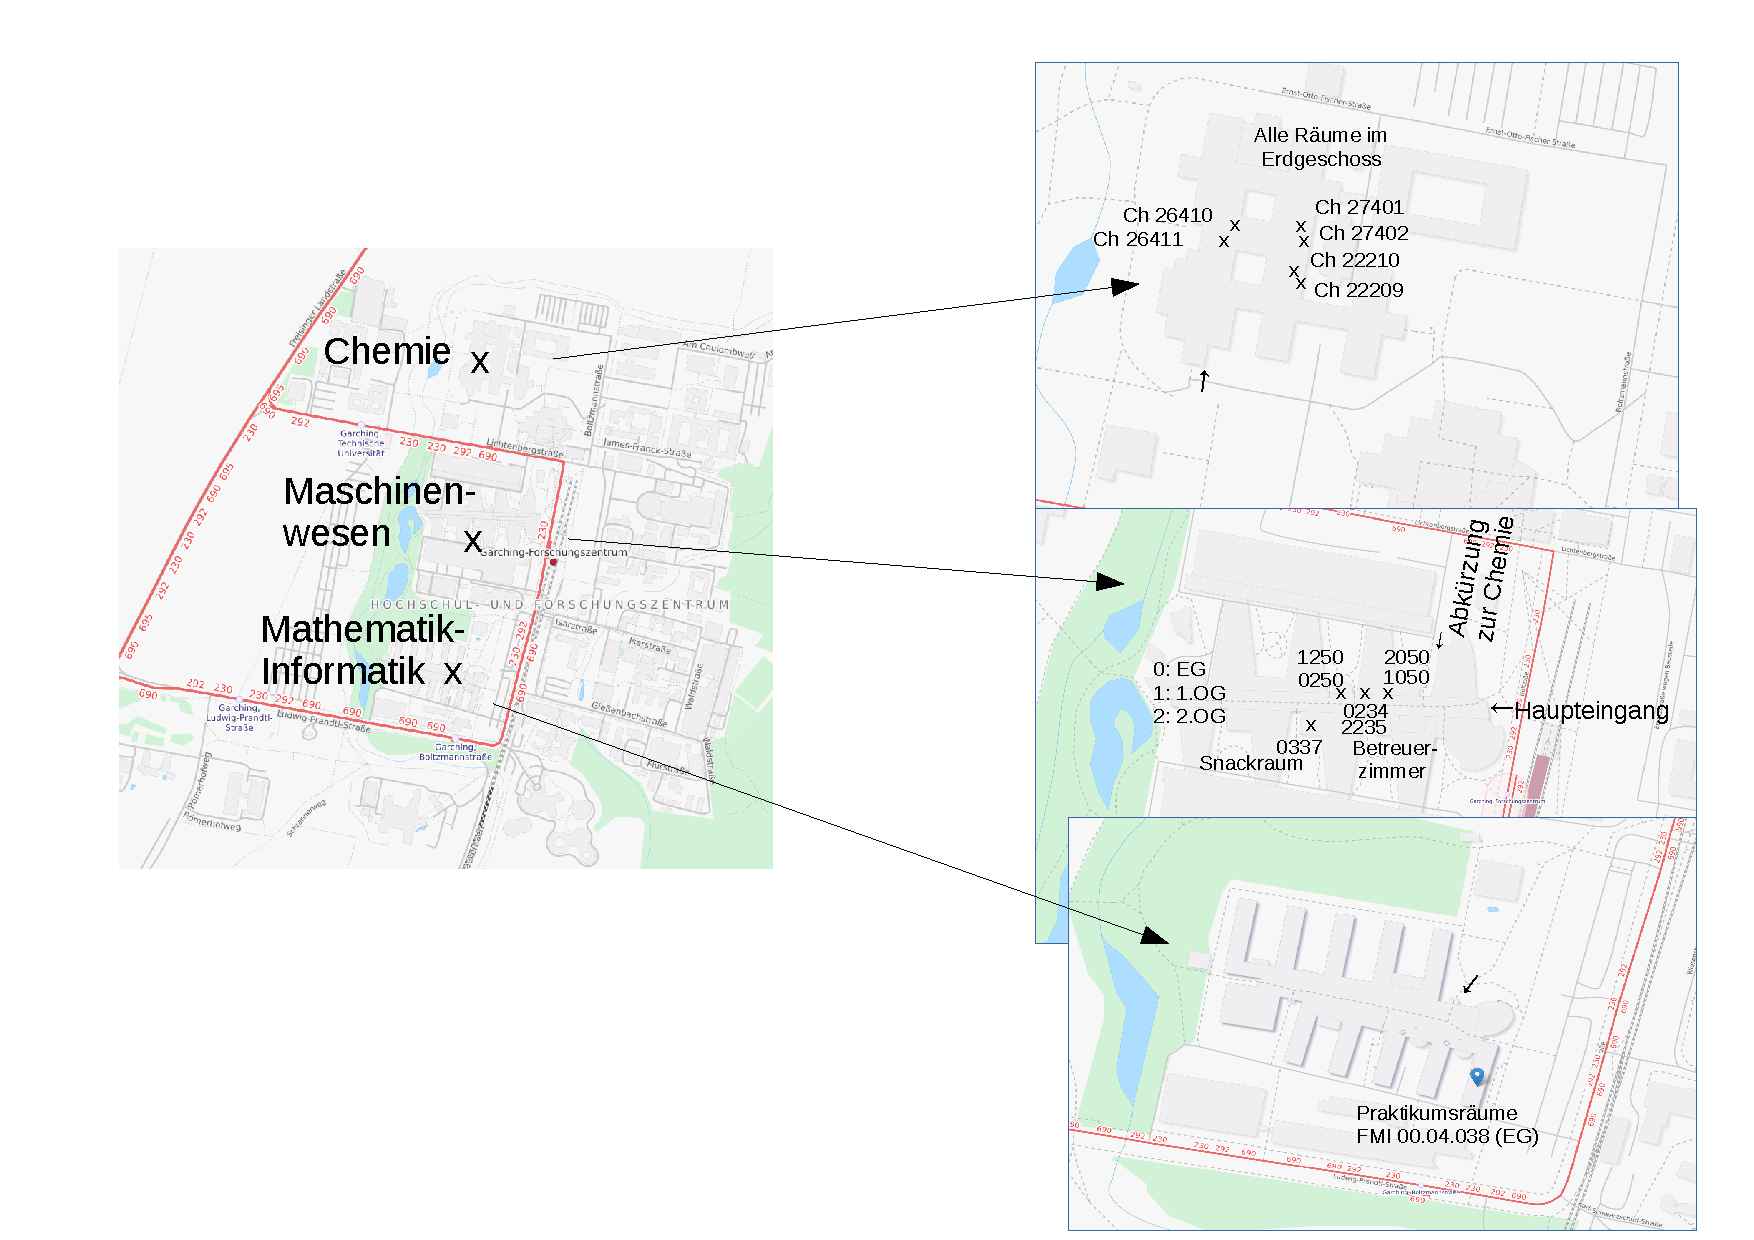
\includegraphics[scale=0.5]{campus_map.pdf}
\end{figure}
\newpage{}\begin{center}{\huge{}\textbf{Stundenplan von Florian Bethge}}\end{center}\textbf{{\large{}Donnerstag}}\nopagebreak \\\begin{tabular} {|p{3cm} p{6cm} p{6cm}| }\hline \textbf{11:30 bis 13:45}&\textbf{Anreise zur TU München}&\textbf{Fakultät Maschinenwesen}\\\hline \textbf{12:00 bis 13:30}&\textbf{Mittagessen}&\textbf{Mensa Garching}\\\hline \textbf{14:00}&\textbf{Begrüßung}&\textbf{CH 26411}\\&Begrüßung, Besprechung des Zeitplans, Ausgabe der individuellen Stundenpläne,...&\\\hline \textbf{14:50 bis 16:20}&\textbf{Quanten- und Atomphysik I}&\textbf{CH 26410}\\&Betreuer: Ismail Achmed-Zade&ca. 28 Teilnehmer\\\hline \textbf{16:40 bis 18:10}&\textbf{Näherungsmethoden}&\textbf{MW 0234}\\&Betreuer: Ilja Göthel&ca. 13 Teilnehmer\\\hline \textbf{18:30}&\textbf{Fahrt zur Jugendherberge}&\textbf{}\\\hline \textbf{19:00}&\textbf{Abendessen}&\textbf{Jugendherberge}\\\hline \end{tabular}\\\vspace{5.00000mm}~\\\textbf{{\large{}Freitag}}\nopagebreak \\\begin{tabular} {|p{3cm} p{6cm} p{6cm}| }\hline \textbf{06:30 bis 09:00}&\textbf{Frühstück}&\textbf{Jugendherberge}\\\hline \textbf{09:00 bis 13:00}&frei&\\\hline \textbf{13:00 bis 14:00}&\textbf{Mittagessen}&\textbf{Mensa Garching}\\\hline \textbf{14:20 bis 15:50}&\textbf{Einführung ins Differenzieren}&\textbf{CH 26411}\\&Betreuer: Ann-Kathrin Raab&ca. 5 Teilnehmer\\\hline \textbf{16:10 bis 17:40}&\textbf{Einführung ins Integrieren}&\textbf{MW 2050}\\&Betreuer: Felix Wechsler&ca. 14 Teilnehmer\\\hline \textbf{18:00 bis 18:20}&\textbf{Erlebnisbericht IPhO}&\textbf{CH 26411}\\\hline \textbf{18:30}&\textbf{Fahrt zur Jugendherberge}&\textbf{}\\\hline \textbf{19:00}&\textbf{Abendessen}&\textbf{Jugendherberge}\\\hline \end{tabular}\\\vspace{5.00000mm}~\\\textbf{{\large{}Samstag}}\nopagebreak \\\begin{tabular} {|p{3cm} p{6cm} p{6cm}| }\hline \textbf{06:30 bis 08:00}&\textbf{Frühstück}&\textbf{Jugendherberge}\\\hline \textbf{08:00}&\textbf{Fahrt zur TU}&\textbf{}\\\hline \textbf{09:00 bis 10:30}&\textbf{Experiment Brennstoffzelle}&\textbf{Praktikum Brennstoffzelle}\\&Betreuer: Aaron Wild&ca. 6 Teilnehmer\\\hline \textbf{10:50 bis 12:20}&\textbf{Klassische Mechanik}&\textbf{MW 1050}\\&Betreuer: Maximilian Marienhagen&ca. 3 Teilnehmer\\\hline \textbf{12:40 bis 14:00}&\textbf{Mittagessen}&\textbf{Fakultät Maschinenwesen}\\\hline \textbf{14:20 bis 15:50}&\textbf{Elektrische Schaltungen}&\textbf{CH 26410}\\&Betreuer: Felix Wechsler&ca. 4 Teilnehmer\\\hline \textbf{16:10 bis 17:40}&\textbf{Aufgabenseminar klassische Mechanik}&\textbf{MW 2050}\\&Betreuer: Aaron Wild&ca. 5 Teilnehmer\\\hline \textbf{18:00 bis 18:20}&\textbf{Vorstellung GYPT}&\textbf{CH 26411}\\\hline \textbf{18:30}&\textbf{Fahrt zur Jugendherberge}&\textbf{}\\\hline \textbf{19:00}&\textbf{Abendessen}&\textbf{Jugendherberge}\\\hline \end{tabular}\\\vspace{5.00000mm}~\\\textbf{{\large{}Sonntag}}\nopagebreak \\\begin{tabular} {|p{3cm} p{6cm} p{6cm}| }\hline \textbf{06:30 bis 08:00}&\textbf{Frühstück}&\textbf{Jugendherberge}\\\hline \textbf{08:00}&\textbf{Fahrt zur TU}&\textbf{}\\\hline \textbf{09:00 bis 10:30}&\textbf{Aufgabenseminar Wärmelehre}&\textbf{CH 22209}\\&Betreuer: Maximilian Marienhagen&ca. 9 Teilnehmer\\\hline \textbf{10:50 bis 12:20}&\textbf{Bestimmung des Brechungskoeffizienten von Plexiglas}&\textbf{MW 0234}\\&Betreuer: Lilith Diringer&ca. 8 Teilnehmer\\\hline \textbf{12:40 bis 13:00}&\textbf{Verabschiedung}&\textbf{CH 26411}\\\hline \textbf{13:00}&\textbf{Individuelle Abreise}&\textbf{}\\\hline \textbf{13:00 bis 14:00}&\textbf{Mittagessen}&\textbf{}\\\hline \end{tabular}\\\vspace{5.00000mm}~\\
Notfallnummern: \\
Sven Jandura: xxxx xxxxxxxxx \\
Johannes Rothe: xxxx xxxxxxxxx \\

\large Hast du Lust, die Andern vom Seminar wiederzusehen?\\
\normalsize Dann komm doch einfach zum \textbf{Vereinstreffen}. Dazu musst du kein Vereinsmitglied sein. Neben interesannten Vorträgen und Exkursionen sind jede Menge Spiel und Spaß geplant. Schau in einem Monat einfach noch mal auf der Website vorbei. Wir freuen uns, wenn du dabei bist.

\begin{figure}[!h]
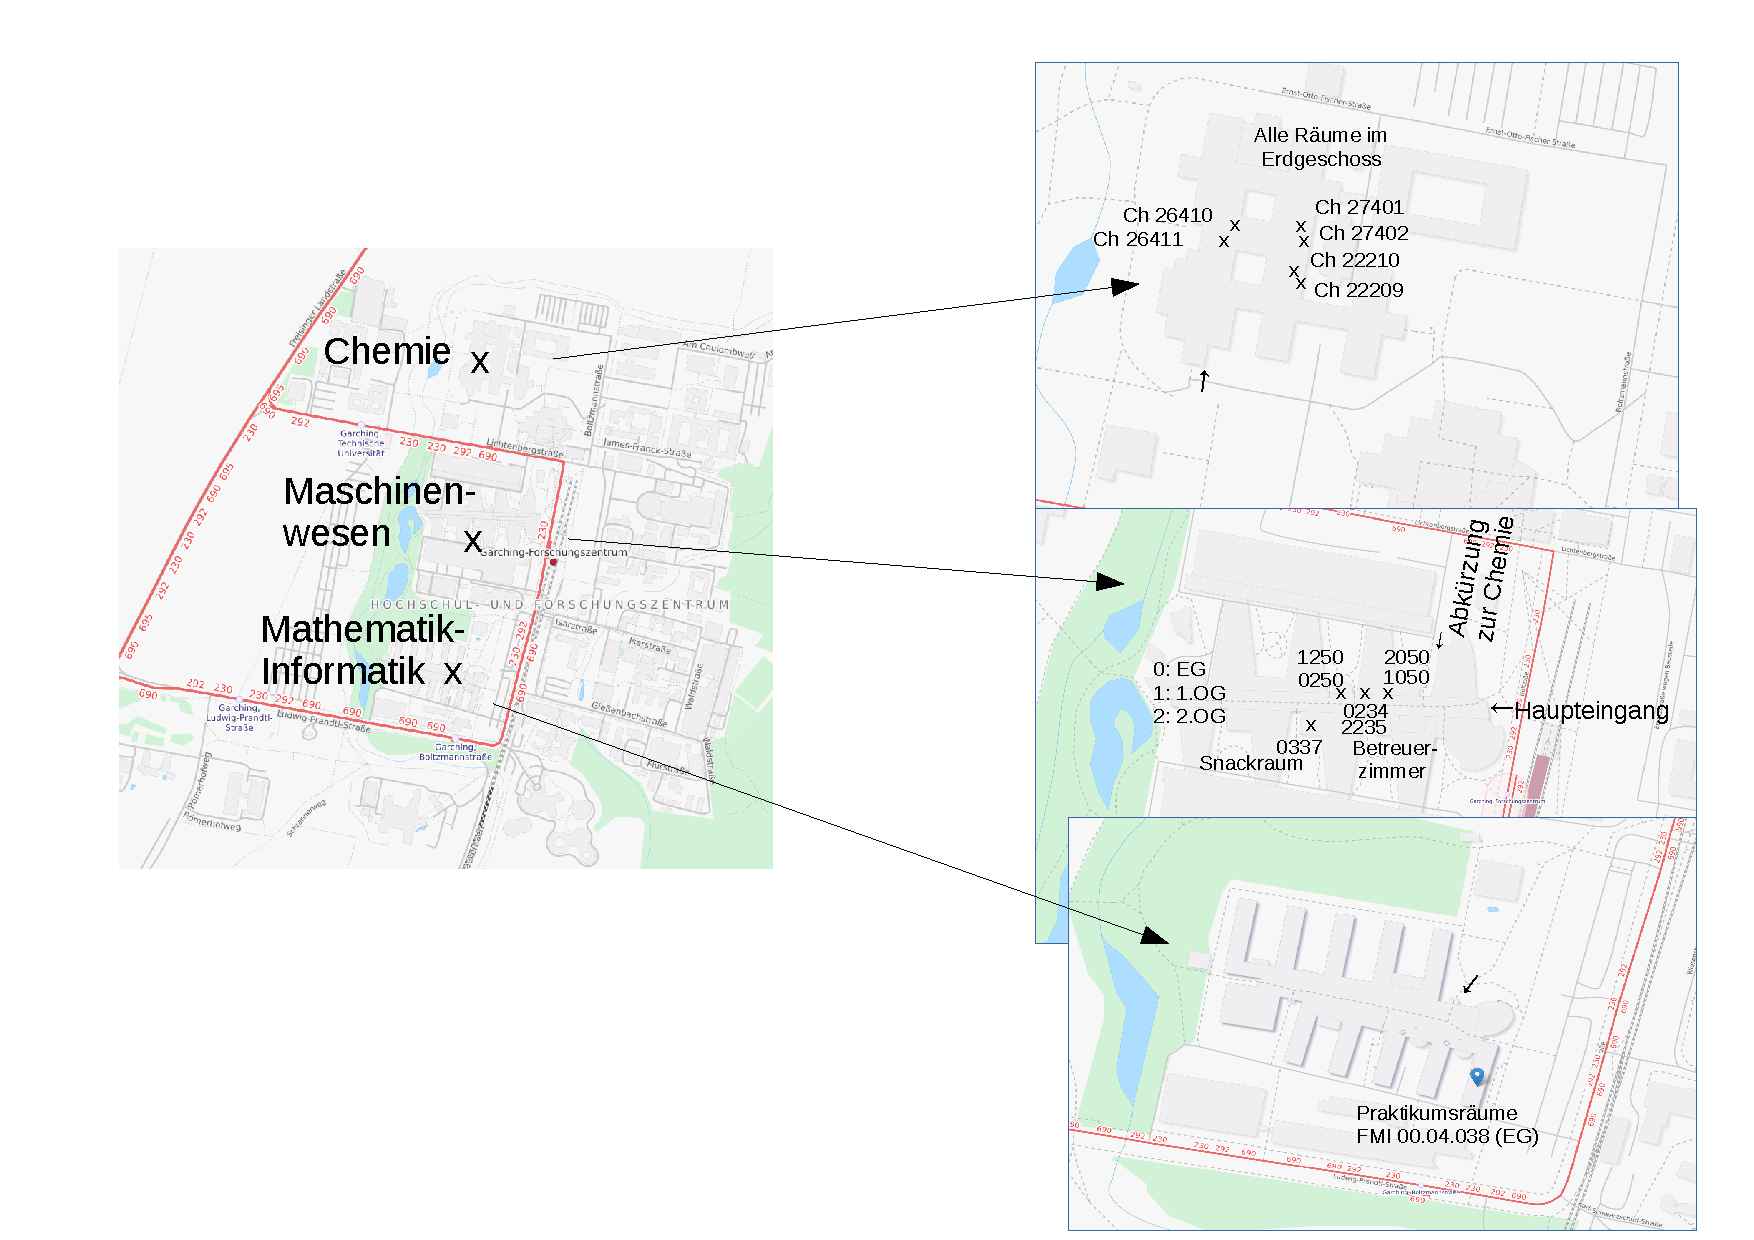
\includegraphics[scale=0.5]{campus_map.pdf}
\end{figure}
\newpage{}\begin{center}{\huge{}\textbf{Stundenplan von Franz Loose}}\end{center}\textbf{{\large{}Donnerstag}}\nopagebreak \\\begin{tabular} {|p{3cm} p{6cm} p{6cm}| }\hline \textbf{11:30 bis 13:45}&\textbf{Anreise zur TU München}&\textbf{Fakultät Maschinenwesen}\\\hline \textbf{12:00 bis 13:30}&\textbf{Mittagessen}&\textbf{Mensa Garching}\\\hline \textbf{14:00}&\textbf{Begrüßung}&\textbf{CH 26411}\\&Begrüßung, Besprechung des Zeitplans, Ausgabe der individuellen Stundenpläne,...&\\\hline \textbf{14:50 bis 16:20}&\textbf{Quanten- und Atomphysik I}&\textbf{CH 26410}\\&Betreuer: Ismail Achmed-Zade&ca. 28 Teilnehmer\\\hline \textbf{16:40 bis 18:10}&\textbf{Einführung ins Integrieren}&\textbf{MW 1050}\\&Betreuer: Johannes Rothe&ca. 14 Teilnehmer\\\hline \textbf{18:30}&\textbf{Fahrt zur Jugendherberge}&\textbf{}\\\hline \textbf{19:00}&\textbf{Abendessen}&\textbf{Jugendherberge}\\\hline \end{tabular}\\\vspace{5.00000mm}~\\\textbf{{\large{}Freitag}}\nopagebreak \\\begin{tabular} {|p{3cm} p{6cm} p{6cm}| }\hline \textbf{06:30 bis 09:00}&\textbf{Frühstück}&\textbf{Jugendherberge}\\\hline \textbf{09:00 bis 13:00}&frei&\\\hline \textbf{13:00 bis 14:00}&\textbf{Mittagessen}&\textbf{Mensa Garching}\\\hline \textbf{14:20 bis 15:50}&\textbf{Experiment spezifische Elektronenladung}&\textbf{Praktikum spezifische Elektronenladung}\\&Betreuer: Felix Wechsler&ca. 6 Teilnehmer\\\hline \textbf{16:10 bis 17:40}&\textbf{Spezielle Relativitätstheorie}&\textbf{MW 1250}\\&Betreuer: Johannes Rothe&ca. 19 Teilnehmer\\\hline \textbf{18:00 bis 18:20}&\textbf{Erlebnisbericht IPhO}&\textbf{CH 26411}\\\hline \textbf{18:30}&\textbf{Fahrt zur Jugendherberge}&\textbf{}\\\hline \textbf{19:00}&\textbf{Abendessen}&\textbf{Jugendherberge}\\\hline \end{tabular}\\\vspace{5.00000mm}~\\\textbf{{\large{}Samstag}}\nopagebreak \\\begin{tabular} {|p{3cm} p{6cm} p{6cm}| }\hline \textbf{06:30 bis 08:00}&\textbf{Frühstück}&\textbf{Jugendherberge}\\\hline \textbf{08:00}&\textbf{Fahrt zur TU}&\textbf{}\\\hline \textbf{09:00 bis 10:30}&\textbf{Elektrodynamik 1}&\textbf{MW 1250}\\&Betreuer: Maximilian Keitel&ca. 21 Teilnehmer\\\hline \textbf{10:50 bis 12:20}&\textbf{Experiment Millikan-Versuch}&\textbf{Praktikum Millikan-Versuch}\\&Betreuer: Samuel Moll&ca. 6 Teilnehmer\\\hline \textbf{12:40 bis 14:00}&\textbf{Mittagessen}&\textbf{Fakultät Maschinenwesen}\\\hline \textbf{14:20 bis 15:50}&\textbf{Thermodynamik 1}&\textbf{MW 1250}\\&Betreuer: Maximilian Marienhagen&ca. 9 Teilnehmer\\\hline \textbf{16:10 bis 17:40}&\textbf{Aufgabenseminar Elektrodynamik}&\textbf{MW 1250}\\&Betreuer: Maximilian Keitel&ca. 8 Teilnehmer\\\hline \textbf{18:00 bis 18:20}&\textbf{Vorstellung GYPT}&\textbf{CH 26411}\\\hline \textbf{18:30}&\textbf{Fahrt zur Jugendherberge}&\textbf{}\\\hline \textbf{19:00}&\textbf{Abendessen}&\textbf{Jugendherberge}\\\hline \end{tabular}\\\vspace{5.00000mm}~\\\textbf{{\large{}Sonntag}}\nopagebreak \\\begin{tabular} {|p{3cm} p{6cm} p{6cm}| }\hline \textbf{06:30 bis 08:00}&\textbf{Frühstück}&\textbf{Jugendherberge}\\\hline \textbf{08:00}&\textbf{Fahrt zur TU}&\textbf{}\\\hline \textbf{09:00 bis 10:30}&\textbf{Aufgabenseminar Wärmelehre}&\textbf{CH 22209}\\&Betreuer: Maximilian Marienhagen&ca. 9 Teilnehmer\\\hline \textbf{10:50 bis 12:20}&\textbf{Rotationsbewegungen}&\textbf{CH 26410}\\&Betreuer: Vincent Grande&ca. 9 Teilnehmer\\\hline \textbf{12:40 bis 13:00}&\textbf{Verabschiedung}&\textbf{CH 26411}\\\hline \textbf{13:00}&\textbf{Individuelle Abreise}&\textbf{}\\\hline \textbf{13:00 bis 14:00}&\textbf{Mittagessen}&\textbf{}\\\hline \end{tabular}\\\vspace{5.00000mm}~\\
Notfallnummern: \\
Sven Jandura: xxxx xxxxxxxxx \\
Johannes Rothe: xxxx xxxxxxxxx \\

\large Hast du Lust, die Andern vom Seminar wiederzusehen?\\
\normalsize Dann komm doch einfach zum \textbf{Vereinstreffen}. Dazu musst du kein Vereinsmitglied sein. Neben interesannten Vorträgen und Exkursionen sind jede Menge Spiel und Spaß geplant. Schau in einem Monat einfach noch mal auf der Website vorbei. Wir freuen uns, wenn du dabei bist.

\begin{figure}[!h]
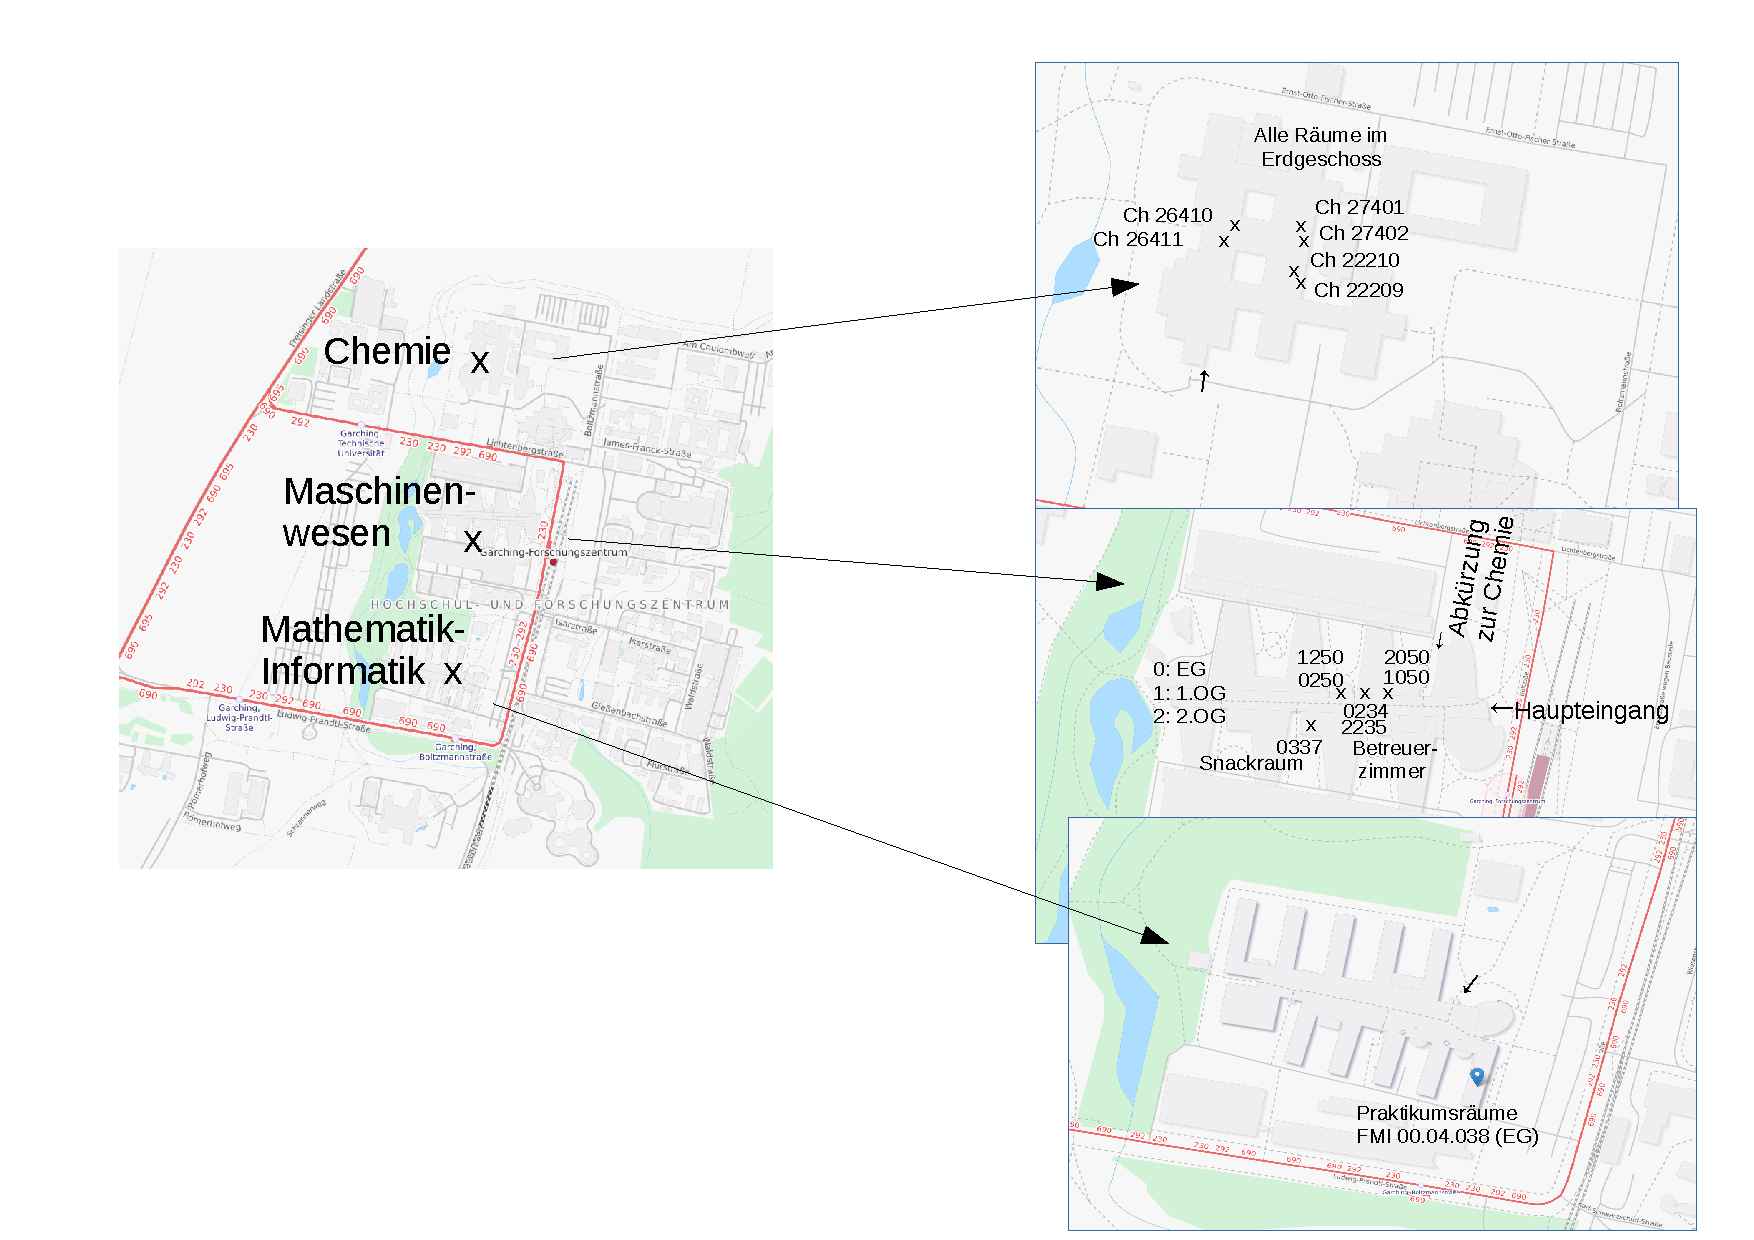
\includegraphics[scale=0.5]{campus_map.pdf}
\end{figure}
\newpage{}\begin{center}{\huge{}\textbf{Stundenplan von Gesa Dünnweber}}\end{center}\textbf{{\large{}Donnerstag}}\nopagebreak \\\begin{tabular} {|p{3cm} p{6cm} p{6cm}| }\hline \textbf{11:30 bis 13:45}&\textbf{Anreise zur TU München}&\textbf{Fakultät Maschinenwesen}\\\hline \textbf{12:00 bis 13:30}&\textbf{Mittagessen}&\textbf{Mensa Garching}\\\hline \textbf{14:00}&\textbf{Begrüßung}&\textbf{CH 26411}\\&Begrüßung, Besprechung des Zeitplans, Ausgabe der individuellen Stundenpläne,...&\\\hline \textbf{14:50 bis 16:20}&\textbf{Einführung ins Differenzieren}&\textbf{MW 1050}\\&Betreuer: Ilja Göthel&ca. 6 Teilnehmer\\\hline \textbf{16:40 bis 18:10}&\textbf{Himmelsmechanik}&\textbf{MW 2050}\\&Betreuer: Lars Dehlwes&ca. 19 Teilnehmer\\\hline \textbf{18:30}&\textbf{Fahrt zur Jugendherberge}&\textbf{}\\\hline \textbf{19:00}&\textbf{Abendessen}&\textbf{Jugendherberge}\\\hline \end{tabular}\\\vspace{5.00000mm}~\\\textbf{{\large{}Freitag}}\nopagebreak \\\begin{tabular} {|p{3cm} p{6cm} p{6cm}| }\hline \textbf{06:30 bis 09:00}&\textbf{Frühstück}&\textbf{Jugendherberge}\\\hline \textbf{09:00 bis 13:00}&\textbf{Besichtigung der Forschungsneutronenquelle FRM II}&\textbf{MW 2050}\\&Betreuer: Felix Wechsler&ca. 28 Teilnehmer\\\hline \textbf{13:00 bis 14:00}&\textbf{Mittagessen}&\textbf{Mensa Garching}\\\hline \textbf{14:20 bis 15:50}&\textbf{Gewöhnliche Differentialgleichungen}&\textbf{MW 1250}\\&Betreuer: Sven Jandura&ca. 20 Teilnehmer\\\hline \textbf{16:10 bis 17:40}&\textbf{Spezielle Relativitätstheorie}&\textbf{MW 1250}\\&Betreuer: Johannes Rothe&ca. 19 Teilnehmer\\\hline \textbf{18:00 bis 18:20}&\textbf{Erlebnisbericht IPhO}&\textbf{CH 26411}\\\hline \textbf{18:30}&\textbf{Fahrt zur Jugendherberge}&\textbf{}\\\hline \textbf{19:00}&\textbf{Abendessen}&\textbf{Jugendherberge}\\\hline \end{tabular}\\\vspace{5.00000mm}~\\\textbf{{\large{}Samstag}}\nopagebreak \\\begin{tabular} {|p{3cm} p{6cm} p{6cm}| }\hline \textbf{06:30 bis 08:00}&\textbf{Frühstück}&\textbf{Jugendherberge}\\\hline \textbf{08:00}&\textbf{Fahrt zur TU}&\textbf{}\\\hline \textbf{09:00 bis 10:30}&\textbf{Experimentieren und Auswerten}&\textbf{CH 26411}\\&Betreuer: Ann-Kathrin Raab&ca. 18 Teilnehmer\\\hline \textbf{10:50 bis 12:20}&\textbf{Quanten- und Atomphysik I}&\textbf{MW 2050}\\&Betreuer: Vitaly Andreev&ca. 13 Teilnehmer\\\hline \textbf{12:40 bis 14:00}&\textbf{Mittagessen}&\textbf{Fakultät Maschinenwesen}\\\hline \textbf{14:20 bis 15:50}&\textbf{Gravitationsbeschleunigung}&\textbf{MW 1050}\\&Betreuer: Ann-Kathrin Raab&ca. 8 Teilnehmer\\\hline \textbf{16:10 bis 17:40}&\textbf{Elektrische Blackboxen}&\textbf{Praktikum Blackboxen}\\&Betreuer: Eugen Dizer&ca. 6 Teilnehmer\\\hline \textbf{18:00 bis 18:20}&\textbf{Vorstellung GYPT}&\textbf{CH 26411}\\\hline \textbf{18:30}&\textbf{Fahrt zur Jugendherberge}&\textbf{}\\\hline \textbf{19:00}&\textbf{Abendessen}&\textbf{Jugendherberge}\\\hline \end{tabular}\\\vspace{5.00000mm}~\\\textbf{{\large{}Sonntag}}\nopagebreak \\\begin{tabular} {|p{3cm} p{6cm} p{6cm}| }\hline \textbf{06:30 bis 08:00}&\textbf{Frühstück}&\textbf{Jugendherberge}\\\hline \textbf{08:00}&\textbf{Fahrt zur TU}&\textbf{}\\\hline \textbf{09:00 bis 10:30}&\textbf{Quanten- und Atomphysik II}&\textbf{MW 1250}\\&Betreuer: Vitaly Andreev&ca. 15 Teilnehmer\\\hline \textbf{10:50 bis 12:20}&\textbf{Aufgabenseminar Quanten- und Atomphysik und Struktur der Materie}&\textbf{MW 1250}\\&Betreuer: Vitaly Andreev&ca. 24 Teilnehmer\\\hline \textbf{12:40 bis 13:00}&\textbf{Verabschiedung}&\textbf{CH 26411}\\\hline \textbf{13:00}&\textbf{Individuelle Abreise}&\textbf{}\\\hline \textbf{13:00 bis 14:00}&\textbf{Mittagessen}&\textbf{}\\\hline \end{tabular}\\\vspace{5.00000mm}~\\
Notfallnummern: \\
Sven Jandura: xxxx xxxxxxxxx \\
Johannes Rothe: xxxx xxxxxxxxx \\

\large Hast du Lust, die Andern vom Seminar wiederzusehen?\\
\normalsize Dann komm doch einfach zum \textbf{Vereinstreffen}. Dazu musst du kein Vereinsmitglied sein. Neben interesannten Vorträgen und Exkursionen sind jede Menge Spiel und Spaß geplant. Schau in einem Monat einfach noch mal auf der Website vorbei. Wir freuen uns, wenn du dabei bist.

\begin{figure}[!h]
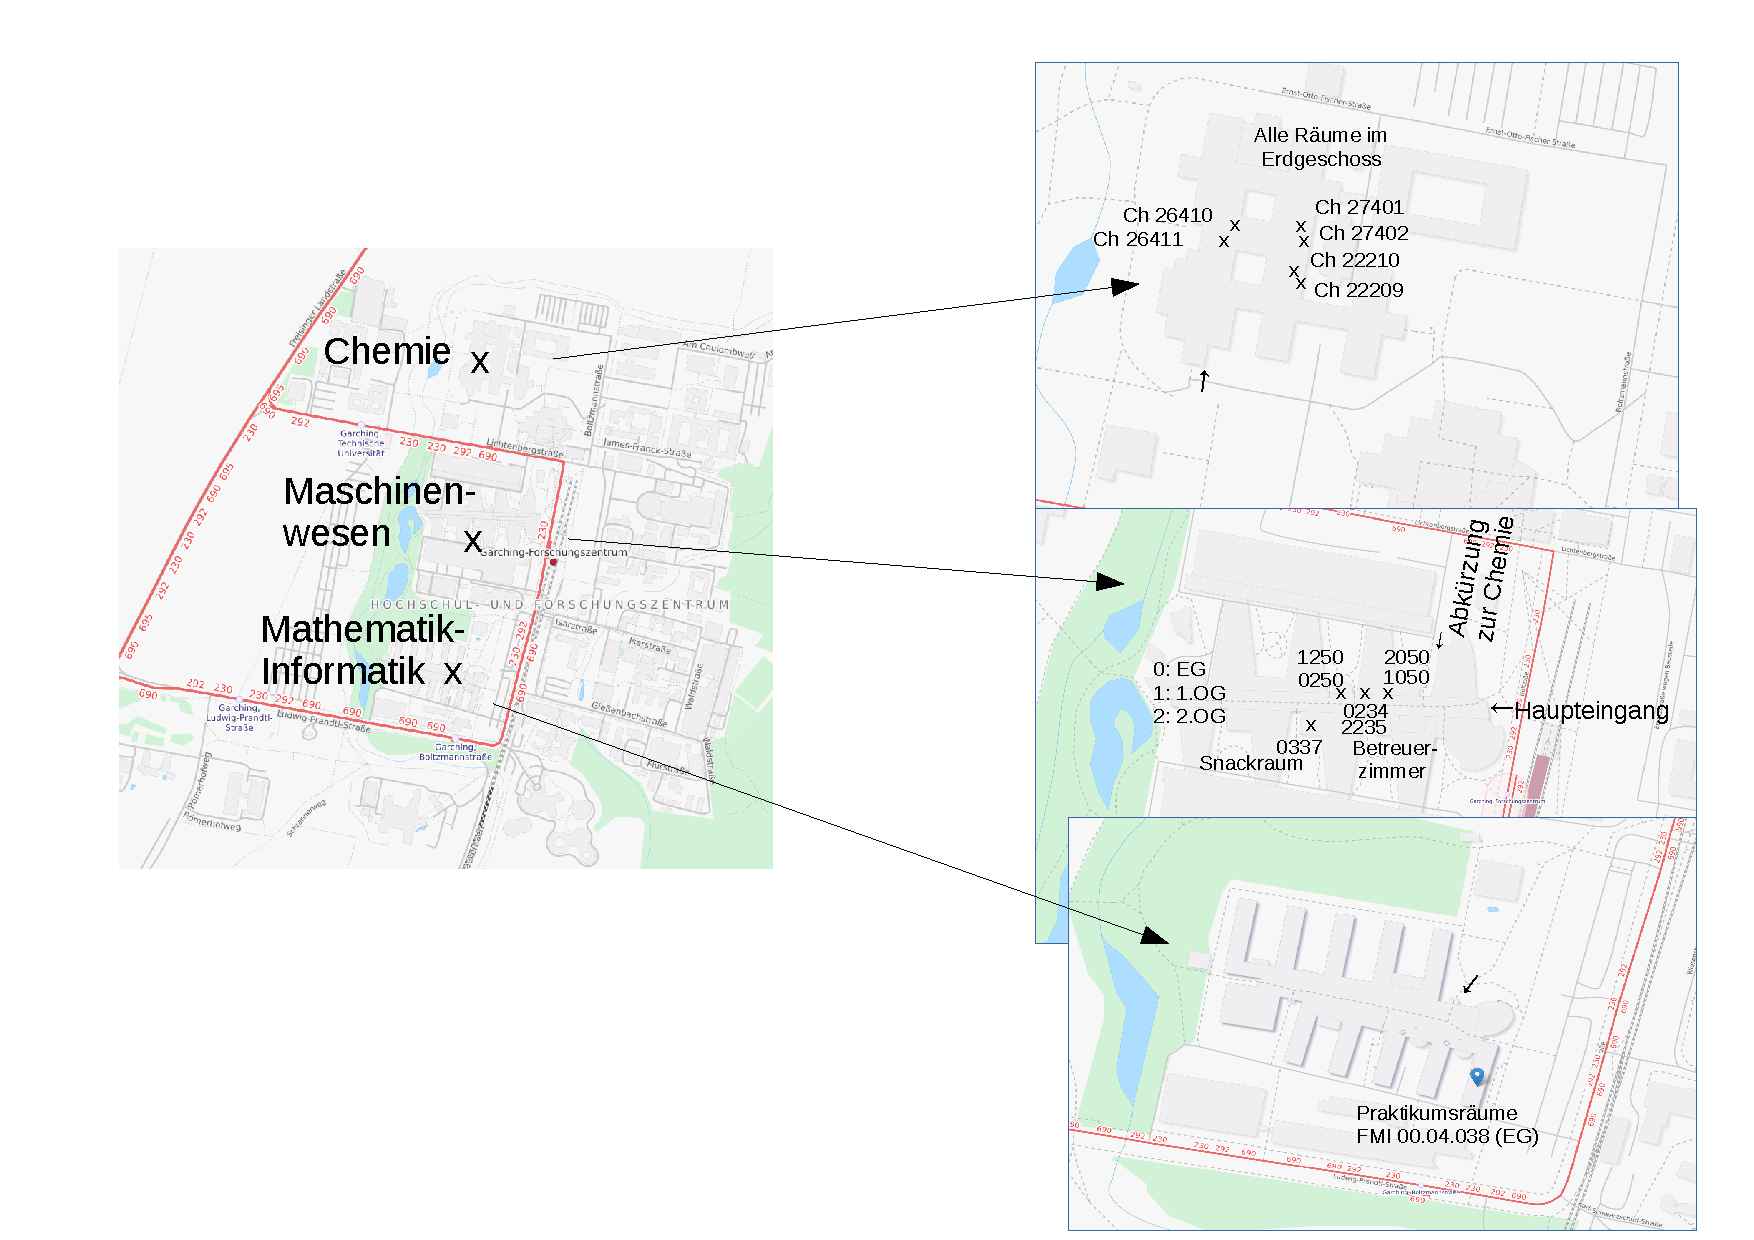
\includegraphics[scale=0.5]{campus_map.pdf}
\end{figure}
\newpage{}\begin{center}{\huge{}\textbf{Stundenplan von Helena Fritschi}}\end{center}\textbf{{\large{}Donnerstag}}\nopagebreak \\\begin{tabular} {|p{3cm} p{6cm} p{6cm}| }\hline \textbf{11:30 bis 13:45}&\textbf{Anreise zur TU München}&\textbf{Fakultät Maschinenwesen}\\\hline \textbf{12:00 bis 13:30}&\textbf{Mittagessen}&\textbf{Mensa Garching}\\\hline \textbf{14:00}&\textbf{Begrüßung}&\textbf{CH 26411}\\&Begrüßung, Besprechung des Zeitplans, Ausgabe der individuellen Stundenpläne,...&\\\hline \textbf{14:50 bis 16:20}&\textbf{Quanten- und Atomphysik I}&\textbf{CH 26410}\\&Betreuer: Ismail Achmed-Zade&ca. 28 Teilnehmer\\\hline \textbf{16:40 bis 18:10}&\textbf{Experimentieren und Auswerten}&\textbf{CH 26411}\\&Betreuer: Ann-Kathrin Raab&ca. 15 Teilnehmer\\\hline \textbf{18:30}&\textbf{Fahrt zur Jugendherberge}&\textbf{}\\\hline \textbf{19:00}&\textbf{Abendessen}&\textbf{Jugendherberge}\\\hline \end{tabular}\\\vspace{5.00000mm}~\\\textbf{{\large{}Freitag}}\nopagebreak \\\begin{tabular} {|p{3cm} p{6cm} p{6cm}| }\hline \textbf{06:30 bis 09:00}&\textbf{Frühstück}&\textbf{Jugendherberge}\\\hline \textbf{09:00 bis 13:00}&frei&\\\hline \textbf{13:00 bis 14:00}&\textbf{Mittagessen}&\textbf{Mensa Garching}\\\hline \textbf{14:20 bis 15:50}&\textbf{Kernphysik}&\textbf{MW 0250}\\&Betreuer: Johannes Rothe&ca. 18 Teilnehmer\\\hline \textbf{16:10 bis 17:40}&\textbf{Experiment spezifische Elektronenladung}&\textbf{Praktikum spezifische Elektronenladung}\\&Betreuer: Felix Wechsler&ca. 6 Teilnehmer\\\hline \textbf{18:00 bis 18:20}&\textbf{Erlebnisbericht IPhO}&\textbf{CH 26411}\\\hline \textbf{18:30}&\textbf{Fahrt zur Jugendherberge}&\textbf{}\\\hline \textbf{19:00}&\textbf{Abendessen}&\textbf{Jugendherberge}\\\hline \end{tabular}\\\vspace{5.00000mm}~\\\textbf{{\large{}Samstag}}\nopagebreak \\\begin{tabular} {|p{3cm} p{6cm} p{6cm}| }\hline \textbf{06:30 bis 08:00}&\textbf{Frühstück}&\textbf{Jugendherberge}\\\hline \textbf{08:00}&\textbf{Fahrt zur TU}&\textbf{}\\\hline \textbf{09:00 bis 10:30}&\textbf{Experiment Millikan-Versuch}&\textbf{Praktikum Millikan-Versuch}\\&Betreuer: Samuel Moll&ca. 6 Teilnehmer\\\hline \textbf{10:50 bis 12:20}&\textbf{Spezielle Relativitätstheorie}&\textbf{MW 0250}\\&Betreuer: Johannes Rothe&ca. 12 Teilnehmer\\\hline \textbf{12:40 bis 14:00}&\textbf{Mittagessen}&\textbf{Fakultät Maschinenwesen}\\\hline \textbf{14:20 bis 15:50}&\textbf{Relativistische Teilchenphysik}&\textbf{CH 22210}\\&Betreuer: Lars Dehlwes&ca. 23 Teilnehmer\\\hline \textbf{16:10 bis 17:40}&\textbf{Quanten- und Atomphysik II}&\textbf{CH 22209}\\&Betreuer: Vitaly Andreev&ca. 28 Teilnehmer\\\hline \textbf{18:00 bis 18:20}&\textbf{Vorstellung GYPT}&\textbf{CH 26411}\\\hline \textbf{18:30}&\textbf{Fahrt zur Jugendherberge}&\textbf{}\\\hline \textbf{19:00}&\textbf{Abendessen}&\textbf{Jugendherberge}\\\hline \end{tabular}\\\vspace{5.00000mm}~\\\textbf{{\large{}Sonntag}}\nopagebreak \\\begin{tabular} {|p{3cm} p{6cm} p{6cm}| }\hline \textbf{06:30 bis 08:00}&\textbf{Frühstück}&\textbf{Jugendherberge}\\\hline \textbf{08:00}&\textbf{Fahrt zur TU}&\textbf{}\\\hline \textbf{09:00 bis 10:30}&\textbf{Wellenoptik}&\textbf{MW 2050}\\&Betreuer: Christopher Pfeiffer&ca. 14 Teilnehmer\\\hline \textbf{10:50 bis 12:20}&\textbf{Aufgabenseminar Quanten- und Atomphysik und Struktur der Materie}&\textbf{MW 1250}\\&Betreuer: Vitaly Andreev&ca. 24 Teilnehmer\\\hline \textbf{12:40 bis 13:00}&\textbf{Verabschiedung}&\textbf{CH 26411}\\\hline \textbf{13:00}&\textbf{Individuelle Abreise}&\textbf{}\\\hline \textbf{13:00 bis 14:00}&\textbf{Mittagessen}&\textbf{}\\\hline \end{tabular}\\\vspace{5.00000mm}~\\
Notfallnummern: \\
Sven Jandura: xxxx xxxxxxxxx \\
Johannes Rothe: xxxx xxxxxxxxx \\

\large Hast du Lust, die Andern vom Seminar wiederzusehen?\\
\normalsize Dann komm doch einfach zum \textbf{Vereinstreffen}. Dazu musst du kein Vereinsmitglied sein. Neben interesannten Vorträgen und Exkursionen sind jede Menge Spiel und Spaß geplant. Schau in einem Monat einfach noch mal auf der Website vorbei. Wir freuen uns, wenn du dabei bist.

\begin{figure}[!h]
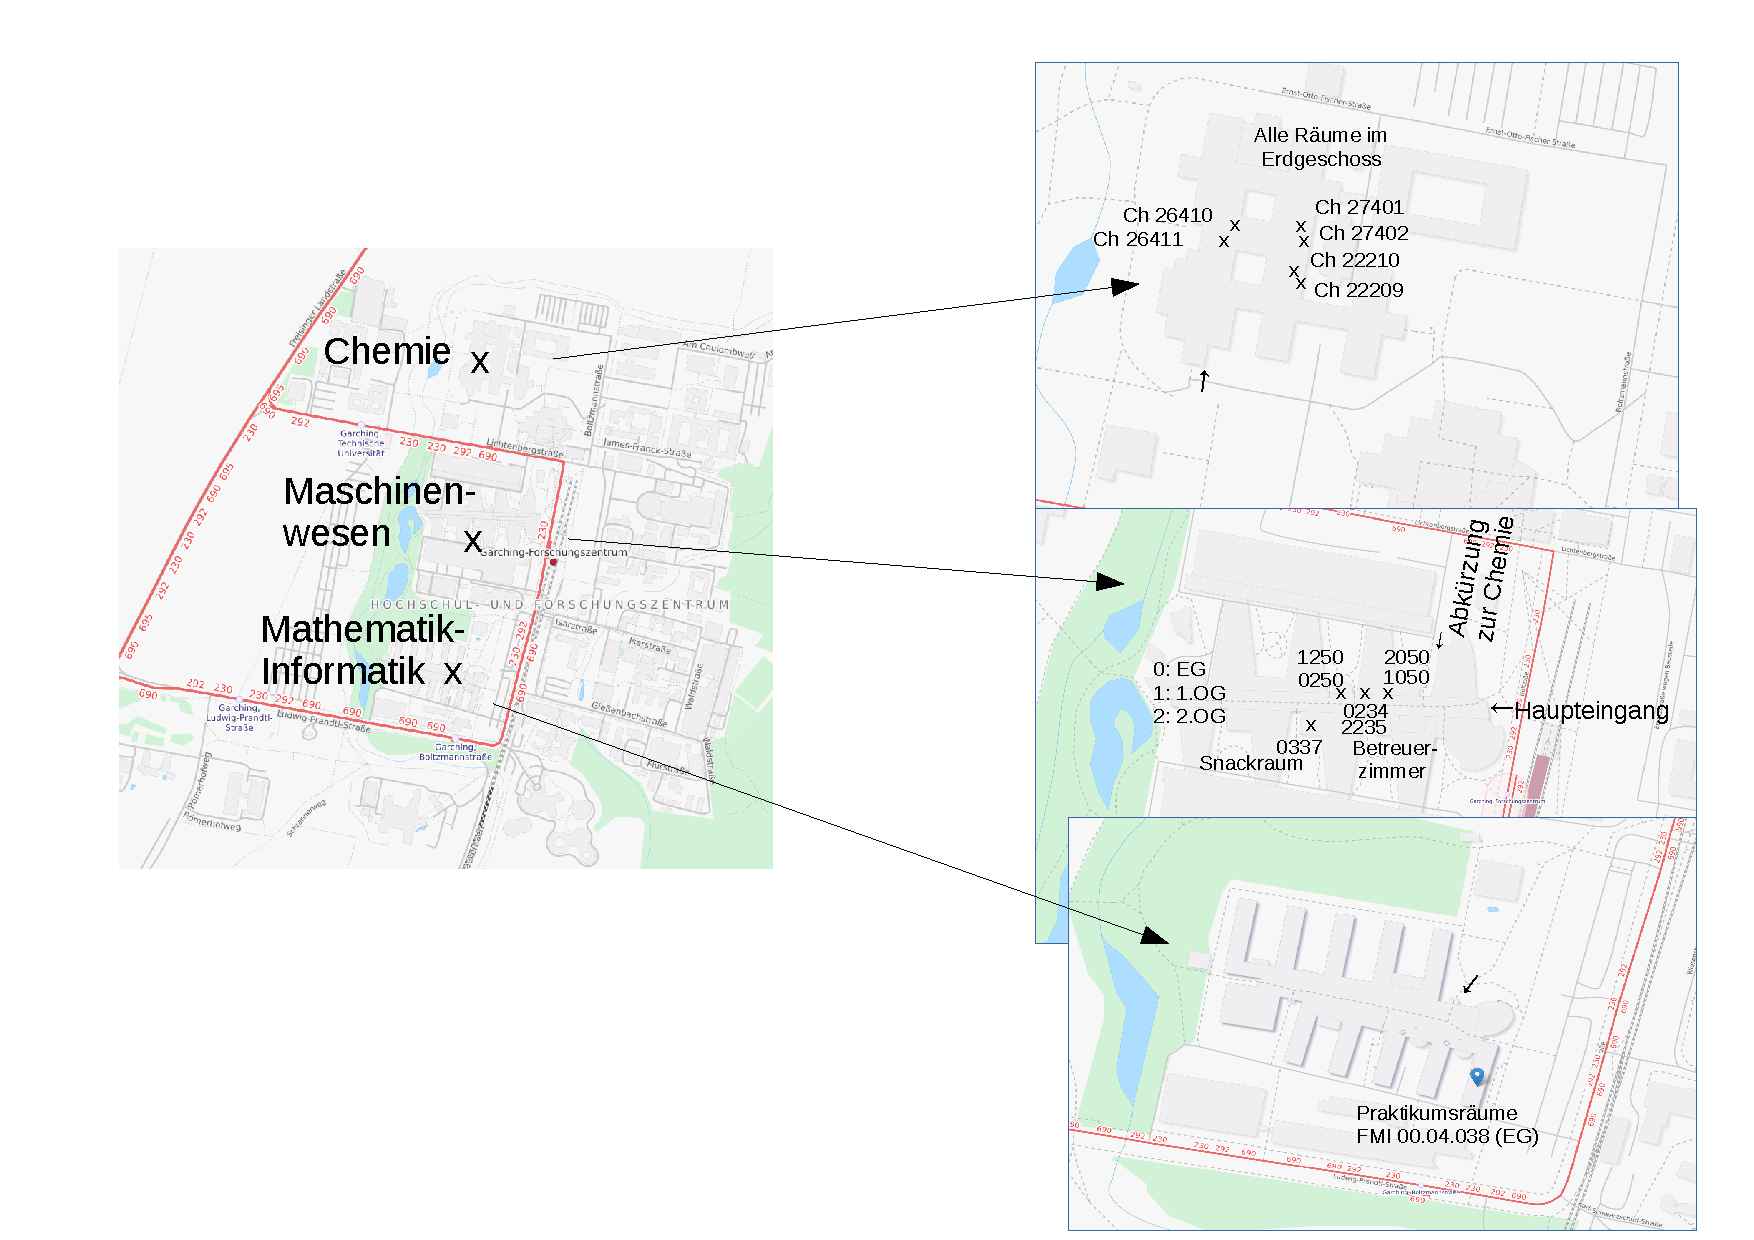
\includegraphics[scale=0.5]{campus_map.pdf}
\end{figure}
\newpage{}\begin{center}{\huge{}\textbf{Stundenplan von Ilka Jaschinski}}\end{center}\textbf{{\large{}Donnerstag}}\nopagebreak \\\begin{tabular} {|p{3cm} p{6cm} p{6cm}| }\hline \textbf{11:30 bis 13:45}&\textbf{Anreise zur TU München}&\textbf{Fakultät Maschinenwesen}\\\hline \textbf{12:00 bis 13:30}&\textbf{Mittagessen}&\textbf{Mensa Garching}\\\hline \textbf{14:00}&\textbf{Begrüßung}&\textbf{CH 26411}\\&Begrüßung, Besprechung des Zeitplans, Ausgabe der individuellen Stundenpläne,...&\\\hline \textbf{14:50 bis 16:20}&\textbf{Quanten- und Atomphysik I}&\textbf{CH 26410}\\&Betreuer: Ismail Achmed-Zade&ca. 28 Teilnehmer\\\hline \textbf{16:40 bis 18:10}&\textbf{Klassische Mechanik}&\textbf{MW 1250}\\&Betreuer: Maximilian Marienhagen&ca. 10 Teilnehmer\\\hline \textbf{18:30}&\textbf{Fahrt zur Jugendherberge}&\textbf{}\\\hline \textbf{19:00}&\textbf{Abendessen}&\textbf{Jugendherberge}\\\hline \end{tabular}\\\vspace{5.00000mm}~\\\textbf{{\large{}Freitag}}\nopagebreak \\\begin{tabular} {|p{3cm} p{6cm} p{6cm}| }\hline \textbf{06:30 bis 09:00}&\textbf{Frühstück}&\textbf{Jugendherberge}\\\hline \textbf{09:00 bis 13:00}&frei&\\\hline \textbf{13:00 bis 14:00}&\textbf{Mittagessen}&\textbf{Mensa Garching}\\\hline \textbf{14:20 bis 15:50}&\textbf{Rotationsbewegungen}&\textbf{MW 1050}\\&Betreuer: Vincent Grande&ca. 6 Teilnehmer\\\hline \textbf{16:10 bis 17:40}&\textbf{Experiment Oszilloskop}&\textbf{Praktikum Oszilloskop}\\&Betreuer: Christopher Pfeiffer&ca. 6 Teilnehmer\\\hline \textbf{18:00 bis 18:20}&\textbf{Erlebnisbericht IPhO}&\textbf{CH 26411}\\\hline \textbf{18:30}&\textbf{Fahrt zur Jugendherberge}&\textbf{}\\\hline \textbf{19:00}&\textbf{Abendessen}&\textbf{Jugendherberge}\\\hline \end{tabular}\\\vspace{5.00000mm}~\\\textbf{{\large{}Samstag}}\nopagebreak \\\begin{tabular} {|p{3cm} p{6cm} p{6cm}| }\hline \textbf{06:30 bis 08:00}&\textbf{Frühstück}&\textbf{Jugendherberge}\\\hline \textbf{08:00}&\textbf{Fahrt zur TU}&\textbf{}\\\hline \textbf{09:00 bis 10:30}&\textbf{Experimentieren und Auswerten}&\textbf{CH 26411}\\&Betreuer: Ann-Kathrin Raab&ca. 18 Teilnehmer\\\hline \textbf{10:50 bis 12:20}&\textbf{Experiment Reversionspendel}&\textbf{Praktikum Reversionspendel}\\&Betreuer: Lilith Diringer&ca. 6 Teilnehmer\\\hline \textbf{12:40 bis 14:00}&\textbf{Mittagessen}&\textbf{Fakultät Maschinenwesen}\\\hline \textbf{14:20 bis 15:50}&\textbf{Gravitationsbeschleunigung}&\textbf{MW 1050}\\&Betreuer: Ann-Kathrin Raab&ca. 8 Teilnehmer\\\hline \textbf{16:10 bis 17:40}&\textbf{Bestimmung des Brechungskoeffizienten von Wasser}&\textbf{MW 0234}\\&Betreuer: Lilith Diringer&ca. 8 Teilnehmer\\\hline \textbf{18:00 bis 18:20}&\textbf{Vorstellung GYPT}&\textbf{CH 26411}\\\hline \textbf{18:30}&\textbf{Fahrt zur Jugendherberge}&\textbf{}\\\hline \textbf{19:00}&\textbf{Abendessen}&\textbf{Jugendherberge}\\\hline \end{tabular}\\\vspace{5.00000mm}~\\\textbf{{\large{}Sonntag}}\nopagebreak \\\begin{tabular} {|p{3cm} p{6cm} p{6cm}| }\hline \textbf{06:30 bis 08:00}&\textbf{Frühstück}&\textbf{Jugendherberge}\\\hline \textbf{08:00}&\textbf{Fahrt zur TU}&\textbf{}\\\hline \textbf{09:00 bis 10:30}&\textbf{Spezielle Relativitätstheorie}&\textbf{MW 0250}\\&Betreuer: Johannes Rothe&ca. 12 Teilnehmer\\\hline \textbf{10:50 bis 12:20}&\textbf{Aufgabenseminar klassische Mechanik}&\textbf{CH 22209}\\&Betreuer: Aaron Wild&ca. 11 Teilnehmer\\\hline \textbf{12:40 bis 13:00}&\textbf{Verabschiedung}&\textbf{CH 26411}\\\hline \textbf{13:00}&\textbf{Individuelle Abreise}&\textbf{}\\\hline \textbf{13:00 bis 14:00}&\textbf{Mittagessen}&\textbf{}\\\hline \end{tabular}\\\vspace{5.00000mm}~\\
Notfallnummern: \\
Sven Jandura: xxxx xxxxxxxxx \\
Johannes Rothe: xxxx xxxxxxxxx \\

\large Hast du Lust, die Andern vom Seminar wiederzusehen?\\
\normalsize Dann komm doch einfach zum \textbf{Vereinstreffen}. Dazu musst du kein Vereinsmitglied sein. Neben interesannten Vorträgen und Exkursionen sind jede Menge Spiel und Spaß geplant. Schau in einem Monat einfach noch mal auf der Website vorbei. Wir freuen uns, wenn du dabei bist.

\begin{figure}[!h]
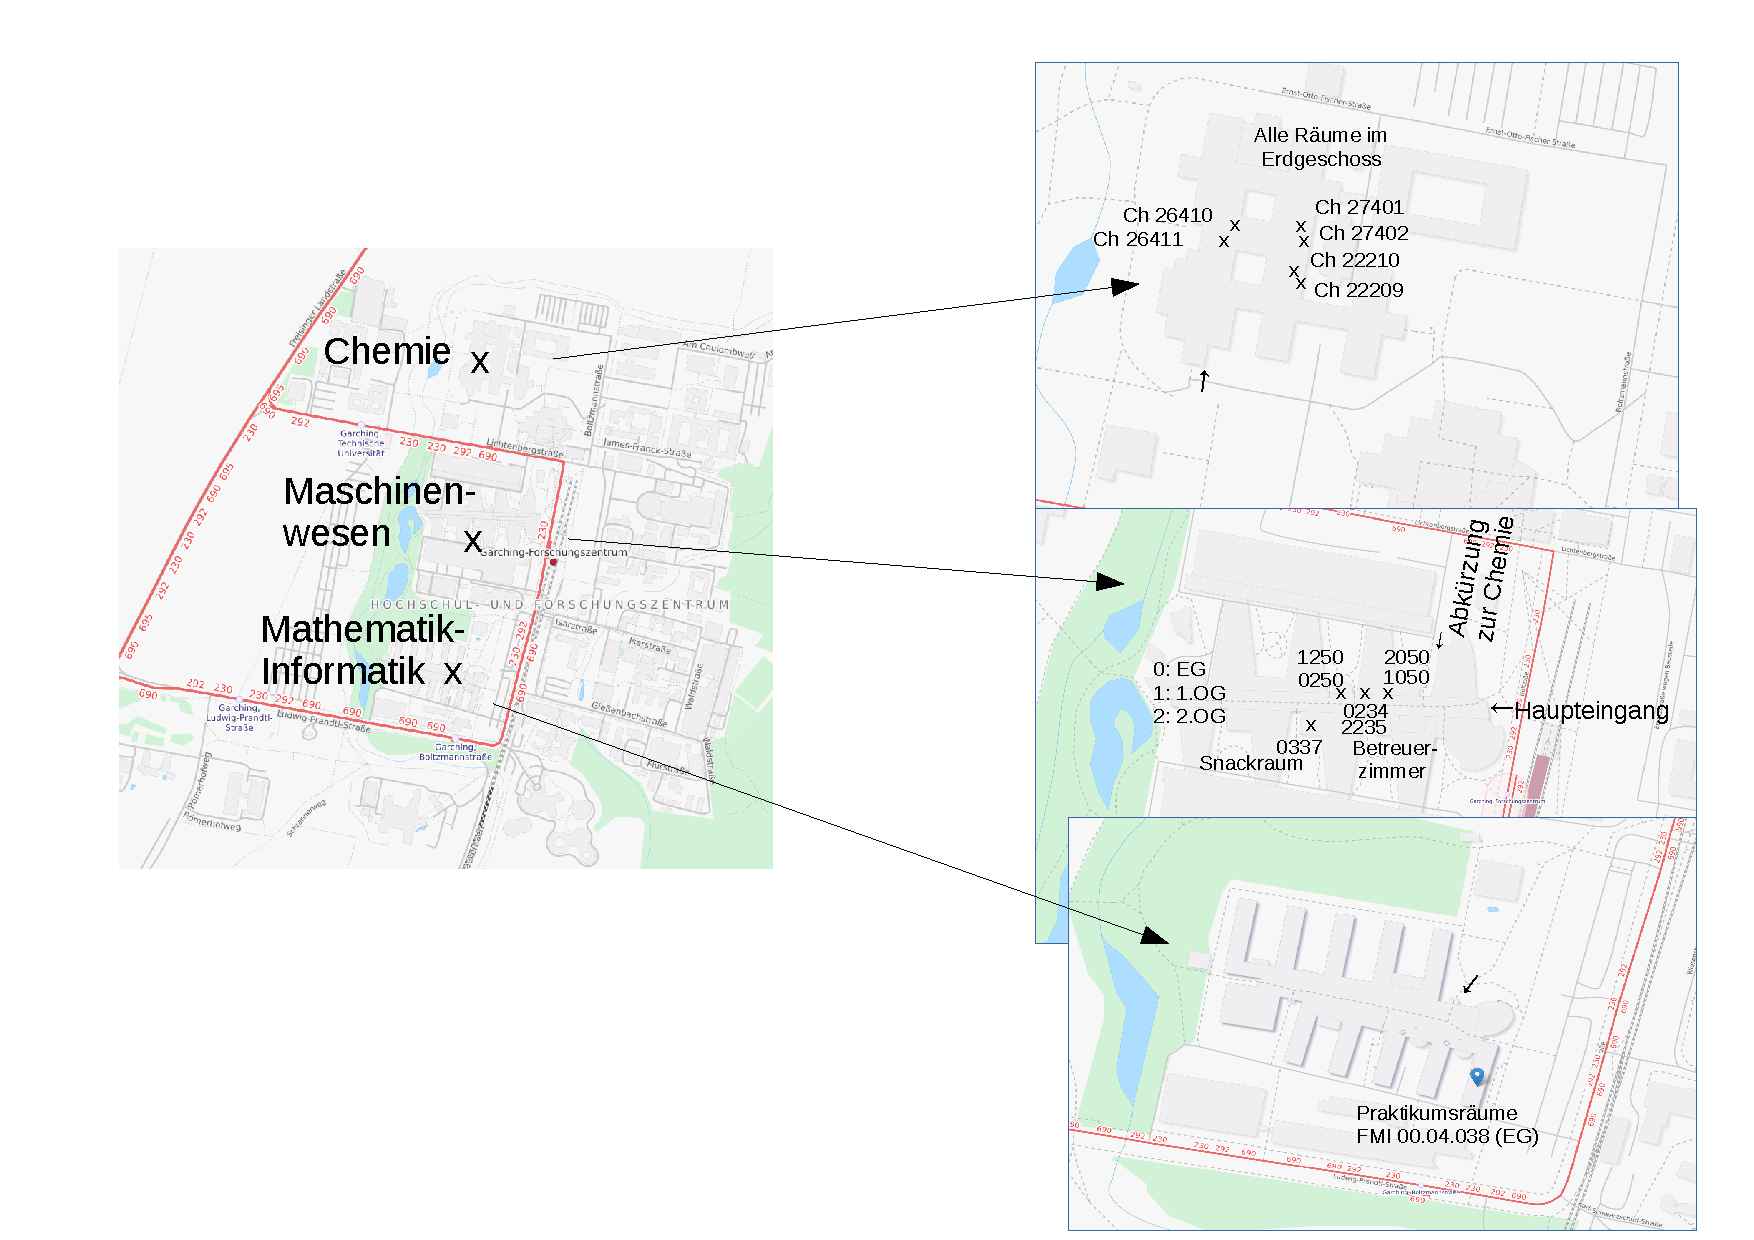
\includegraphics[scale=0.5]{campus_map.pdf}
\end{figure}
\newpage{}\begin{center}{\huge{}\textbf{Stundenplan von Jana Hötte}}\end{center}\textbf{{\large{}Donnerstag}}\nopagebreak \\\begin{tabular} {|p{3cm} p{6cm} p{6cm}| }\hline \textbf{11:30 bis 13:45}&\textbf{Anreise zur TU München}&\textbf{Fakultät Maschinenwesen}\\\hline \textbf{12:00 bis 13:30}&\textbf{Mittagessen}&\textbf{Mensa Garching}\\\hline \textbf{14:00}&\textbf{Begrüßung}&\textbf{CH 26411}\\&Begrüßung, Besprechung des Zeitplans, Ausgabe der individuellen Stundenpläne,...&\\\hline \textbf{14:50 bis 16:20}&frei&\\\hline \textbf{16:40 bis 18:10}&frei&\\\hline \textbf{18:30}&\textbf{Fahrt zur Jugendherberge}&\textbf{}\\\hline \textbf{19:00}&\textbf{Abendessen}&\textbf{Jugendherberge}\\\hline \end{tabular}\\\vspace{5.00000mm}~\\\textbf{{\large{}Freitag}}\nopagebreak \\\begin{tabular} {|p{3cm} p{6cm} p{6cm}| }\hline \textbf{06:30 bis 09:00}&\textbf{Frühstück}&\textbf{Jugendherberge}\\\hline \textbf{09:00 bis 13:00}&frei&\\\hline \textbf{13:00 bis 14:00}&\textbf{Mittagessen}&\textbf{Mensa Garching}\\\hline \textbf{14:20 bis 15:50}&\textbf{Experiment Brückenschaltung}&\textbf{Praktikum Brückenschaltung}\\&Betreuer: Martin Großhauser&ca. 6 Teilnehmer\\\hline \textbf{16:10 bis 17:40}&\textbf{Experiment Magnetismus}&\textbf{Praktikum Magnetismus}\\&Betreuer: Lars Dehlwes&ca. 6 Teilnehmer\\\hline \textbf{18:00 bis 18:20}&\textbf{Erlebnisbericht IPhO}&\textbf{CH 26411}\\\hline \textbf{18:30}&\textbf{Fahrt zur Jugendherberge}&\textbf{}\\\hline \textbf{19:00}&\textbf{Abendessen}&\textbf{Jugendherberge}\\\hline \end{tabular}\\\vspace{5.00000mm}~\\\textbf{{\large{}Samstag}}\nopagebreak \\\begin{tabular} {|p{3cm} p{6cm} p{6cm}| }\hline \textbf{06:30 bis 08:00}&\textbf{Frühstück}&\textbf{Jugendherberge}\\\hline \textbf{08:00}&\textbf{Fahrt zur TU}&\textbf{}\\\hline \textbf{09:00 bis 10:30}&\textbf{Aufgabenseminar klassische Mechanik}&\textbf{MW 0234}\\&Betreuer: Maximilian Marienhagen&ca. 5 Teilnehmer\\\hline \textbf{10:50 bis 12:20}&\textbf{Experiment Reversionspendel}&\textbf{Praktikum Reversionspendel}\\&Betreuer: Lilith Diringer&ca. 6 Teilnehmer\\\hline \textbf{12:40 bis 14:00}&\textbf{Mittagessen}&\textbf{Fakultät Maschinenwesen}\\\hline \textbf{14:20 bis 15:50}&\textbf{Gravitationsbeschleunigung}&\textbf{MW 1050}\\&Betreuer: Ann-Kathrin Raab&ca. 8 Teilnehmer\\\hline \textbf{16:10 bis 17:40}&\textbf{Himmelsmechanik}&\textbf{CH 22210}\\&Betreuer: Lars Dehlwes&ca. 10 Teilnehmer\\\hline \textbf{18:00 bis 18:20}&\textbf{Vorstellung GYPT}&\textbf{CH 26411}\\\hline \textbf{18:30}&\textbf{Fahrt zur Jugendherberge}&\textbf{}\\\hline \textbf{19:00}&\textbf{Abendessen}&\textbf{Jugendherberge}\\\hline \end{tabular}\\\vspace{5.00000mm}~\\\textbf{{\large{}Sonntag}}\nopagebreak \\\begin{tabular} {|p{3cm} p{6cm} p{6cm}| }\hline \textbf{06:30 bis 08:00}&\textbf{Frühstück}&\textbf{Jugendherberge}\\\hline \textbf{08:00}&\textbf{Fahrt zur TU}&\textbf{}\\\hline \textbf{09:00 bis 10:30}&\textbf{Aufgabenseminar Wärmelehre}&\textbf{CH 22209}\\&Betreuer: Maximilian Marienhagen&ca. 9 Teilnehmer\\\hline \textbf{10:50 bis 12:20}&\textbf{Wellenoptik}&\textbf{MW 0250}\\&Betreuer: Christopher Pfeiffer&ca. 12 Teilnehmer\\\hline \textbf{12:40 bis 13:00}&\textbf{Verabschiedung}&\textbf{CH 26411}\\\hline \textbf{13:00}&\textbf{Individuelle Abreise}&\textbf{}\\\hline \textbf{13:00 bis 14:00}&\textbf{Mittagessen}&\textbf{}\\\hline \end{tabular}\\\vspace{5.00000mm}~\\
Notfallnummern: \\
Sven Jandura: xxxx xxxxxxxxx \\
Johannes Rothe: xxxx xxxxxxxxx \\

\large Hast du Lust, die Andern vom Seminar wiederzusehen?\\
\normalsize Dann komm doch einfach zum \textbf{Vereinstreffen}. Dazu musst du kein Vereinsmitglied sein. Neben interesannten Vorträgen und Exkursionen sind jede Menge Spiel und Spaß geplant. Schau in einem Monat einfach noch mal auf der Website vorbei. Wir freuen uns, wenn du dabei bist.

\begin{figure}[!h]
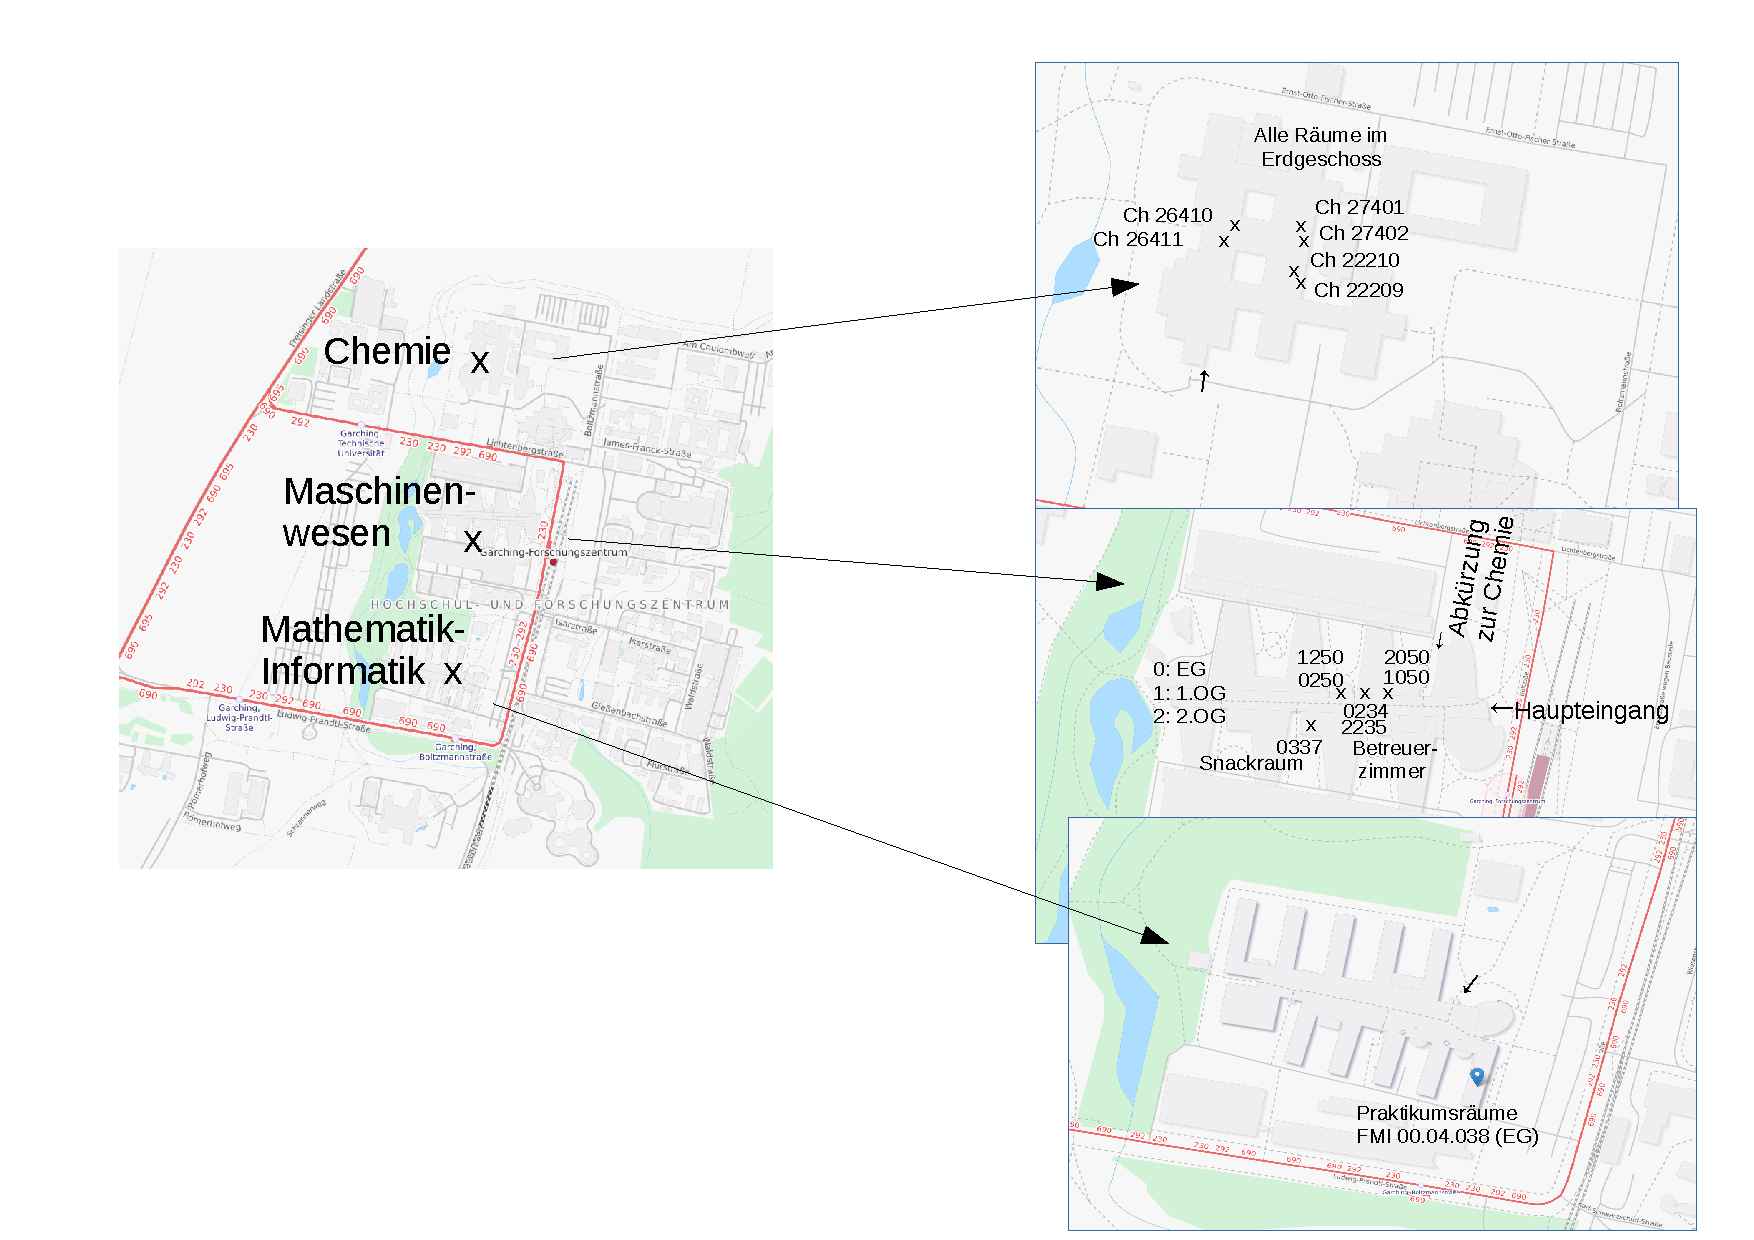
\includegraphics[scale=0.5]{campus_map.pdf}
\end{figure}
\newpage{}\begin{center}{\huge{}\textbf{Stundenplan von Jann Weidlich}}\end{center}\textbf{{\large{}Donnerstag}}\nopagebreak \\\begin{tabular} {|p{3cm} p{6cm} p{6cm}| }\hline \textbf{11:30 bis 13:45}&\textbf{Anreise zur TU München}&\textbf{Fakultät Maschinenwesen}\\\hline \textbf{12:00 bis 13:30}&\textbf{Mittagessen}&\textbf{Mensa Garching}\\\hline \textbf{14:00}&\textbf{Begrüßung}&\textbf{CH 26411}\\&Begrüßung, Besprechung des Zeitplans, Ausgabe der individuellen Stundenpläne,...&\\\hline \textbf{14:50 bis 16:20}&\textbf{Quanten- und Atomphysik I}&\textbf{CH 26410}\\&Betreuer: Ismail Achmed-Zade&ca. 28 Teilnehmer\\\hline \textbf{16:40 bis 18:10}&\textbf{Näherungsmethoden}&\textbf{MW 0234}\\&Betreuer: Ilja Göthel&ca. 13 Teilnehmer\\\hline \textbf{18:30}&\textbf{Fahrt zur Jugendherberge}&\textbf{}\\\hline \textbf{19:00}&\textbf{Abendessen}&\textbf{Jugendherberge}\\\hline \end{tabular}\\\vspace{5.00000mm}~\\\textbf{{\large{}Freitag}}\nopagebreak \\\begin{tabular} {|p{3cm} p{6cm} p{6cm}| }\hline \textbf{06:30 bis 09:00}&\textbf{Frühstück}&\textbf{Jugendherberge}\\\hline \textbf{09:00 bis 13:00}&\textbf{Besichtigung der Forschungsneutronenquelle FRM II}&\textbf{MW 2050}\\&Betreuer: Felix Wechsler&ca. 28 Teilnehmer\\\hline \textbf{13:00 bis 14:00}&\textbf{Mittagessen}&\textbf{Mensa Garching}\\\hline \textbf{14:20 bis 15:50}&\textbf{Gewöhnliche Differentialgleichungen}&\textbf{MW 1250}\\&Betreuer: Sven Jandura&ca. 20 Teilnehmer\\\hline \textbf{16:10 bis 17:40}&\textbf{Spezielle Relativitätstheorie}&\textbf{MW 1250}\\&Betreuer: Johannes Rothe&ca. 19 Teilnehmer\\\hline \textbf{18:00 bis 18:20}&\textbf{Erlebnisbericht IPhO}&\textbf{CH 26411}\\\hline \textbf{18:30}&\textbf{Fahrt zur Jugendherberge}&\textbf{}\\\hline \textbf{19:00}&\textbf{Abendessen}&\textbf{Jugendherberge}\\\hline \end{tabular}\\\vspace{5.00000mm}~\\\textbf{{\large{}Samstag}}\nopagebreak \\\begin{tabular} {|p{3cm} p{6cm} p{6cm}| }\hline \textbf{06:30 bis 08:00}&\textbf{Frühstück}&\textbf{Jugendherberge}\\\hline \textbf{08:00}&\textbf{Fahrt zur TU}&\textbf{}\\\hline \textbf{09:00 bis 10:30}&\textbf{Experimentieren und Auswerten}&\textbf{CH 26411}\\&Betreuer: Ann-Kathrin Raab&ca. 18 Teilnehmer\\\hline \textbf{10:50 bis 12:20}&\textbf{Experiment Millikan-Versuch}&\textbf{Praktikum Millikan-Versuch}\\&Betreuer: Samuel Moll&ca. 6 Teilnehmer\\\hline \textbf{12:40 bis 14:00}&\textbf{Mittagessen}&\textbf{Fakultät Maschinenwesen}\\\hline \textbf{14:20 bis 15:50}&\textbf{Elektrodynamik 2}&\textbf{MW 2050}\\&Betreuer: Maximilian Keitel&ca. 6 Teilnehmer\\\hline \textbf{16:10 bis 17:40}&\textbf{Komplexe Wechselstromrechnung}&\textbf{MW 0250}\\&Betreuer: Vincent Grande&ca. 13 Teilnehmer\\\hline \textbf{18:00 bis 18:20}&\textbf{Vorstellung GYPT}&\textbf{CH 26411}\\\hline \textbf{18:30}&\textbf{Fahrt zur Jugendherberge}&\textbf{}\\\hline \textbf{19:00}&\textbf{Abendessen}&\textbf{Jugendherberge}\\\hline \end{tabular}\\\vspace{5.00000mm}~\\\textbf{{\large{}Sonntag}}\nopagebreak \\\begin{tabular} {|p{3cm} p{6cm} p{6cm}| }\hline \textbf{06:30 bis 08:00}&\textbf{Frühstück}&\textbf{Jugendherberge}\\\hline \textbf{08:00}&\textbf{Fahrt zur TU}&\textbf{}\\\hline \textbf{09:00 bis 10:30}&\textbf{Quanten- und Atomphysik II}&\textbf{MW 1250}\\&Betreuer: Vitaly Andreev&ca. 15 Teilnehmer\\\hline \textbf{10:50 bis 12:20}&\textbf{Aufgabenseminar Quanten- und Atomphysik und Struktur der Materie}&\textbf{MW 1250}\\&Betreuer: Vitaly Andreev&ca. 24 Teilnehmer\\\hline \textbf{12:40 bis 13:00}&\textbf{Verabschiedung}&\textbf{CH 26411}\\\hline \textbf{13:00}&\textbf{Individuelle Abreise}&\textbf{}\\\hline \textbf{13:00 bis 14:00}&\textbf{Mittagessen}&\textbf{}\\\hline \end{tabular}\\\vspace{5.00000mm}~\\
Notfallnummern: \\
Sven Jandura: xxxx xxxxxxxxx \\
Johannes Rothe: xxxx xxxxxxxxx \\

\large Hast du Lust, die Andern vom Seminar wiederzusehen?\\
\normalsize Dann komm doch einfach zum \textbf{Vereinstreffen}. Dazu musst du kein Vereinsmitglied sein. Neben interesannten Vorträgen und Exkursionen sind jede Menge Spiel und Spaß geplant. Schau in einem Monat einfach noch mal auf der Website vorbei. Wir freuen uns, wenn du dabei bist.

\begin{figure}[!h]
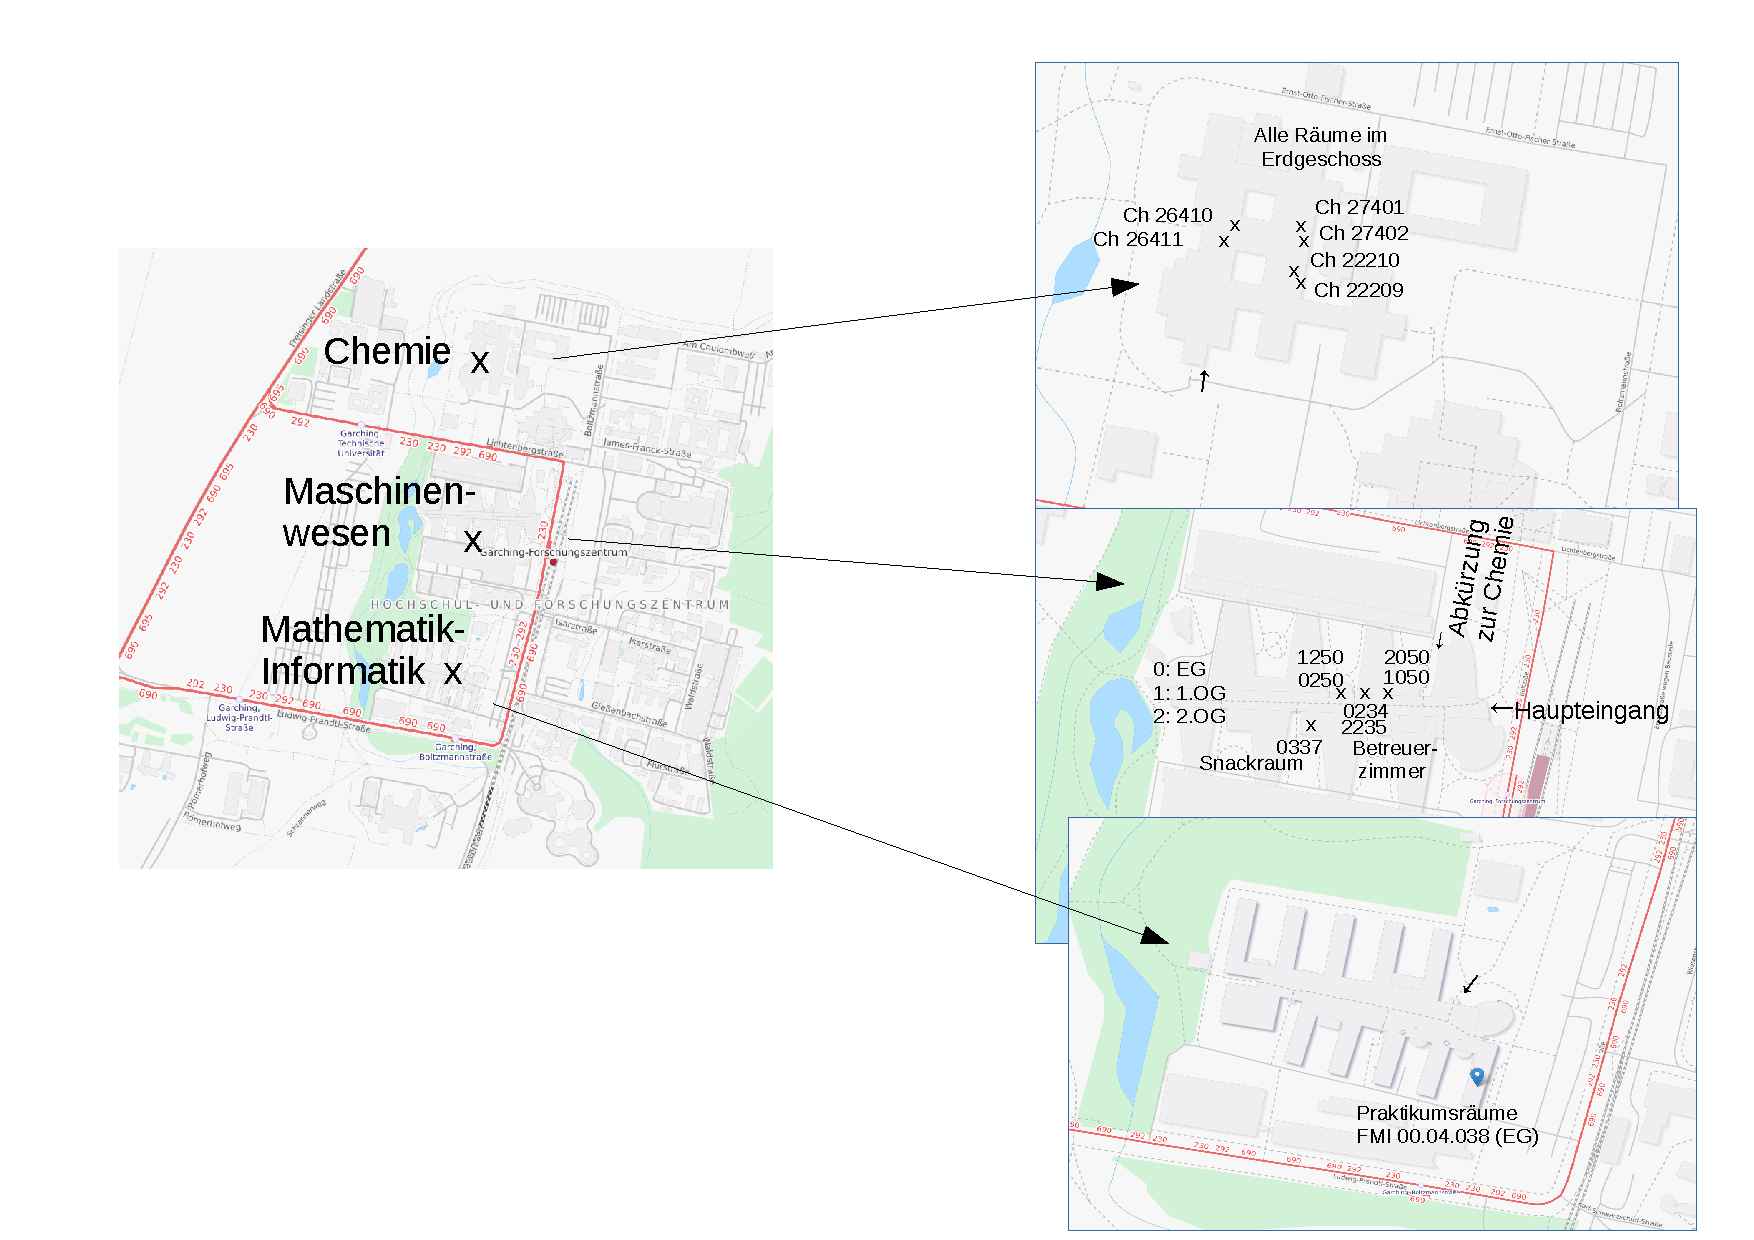
\includegraphics[scale=0.5]{campus_map.pdf}
\end{figure}
\newpage{}\begin{center}{\huge{}\textbf{Stundenplan von Jean-Baptiste Bellynck}}\end{center}\textbf{{\large{}Donnerstag}}\nopagebreak \\\begin{tabular} {|p{3cm} p{6cm} p{6cm}| }\hline \textbf{11:30 bis 13:45}&\textbf{Anreise zur TU München}&\textbf{Fakultät Maschinenwesen}\\\hline \textbf{12:00 bis 13:30}&\textbf{Mittagessen}&\textbf{Mensa Garching}\\\hline \textbf{14:00}&\textbf{Begrüßung}&\textbf{CH 26411}\\&Begrüßung, Besprechung des Zeitplans, Ausgabe der individuellen Stundenpläne,...&\\\hline \textbf{14:50 bis 16:20}&\textbf{Quanten- und Atomphysik I}&\textbf{CH 26410}\\&Betreuer: Ismail Achmed-Zade&ca. 28 Teilnehmer\\\hline \textbf{16:40 bis 18:10}&\textbf{Einführung ins Integrieren}&\textbf{MW 1050}\\&Betreuer: Johannes Rothe&ca. 14 Teilnehmer\\\hline \textbf{18:30}&\textbf{Fahrt zur Jugendherberge}&\textbf{}\\\hline \textbf{19:00}&\textbf{Abendessen}&\textbf{Jugendherberge}\\\hline \end{tabular}\\\vspace{5.00000mm}~\\\textbf{{\large{}Freitag}}\nopagebreak \\\begin{tabular} {|p{3cm} p{6cm} p{6cm}| }\hline \textbf{06:30 bis 09:00}&\textbf{Frühstück}&\textbf{Jugendherberge}\\\hline \textbf{09:00 bis 13:00}&\textbf{Besichtigung der Forschungsneutronenquelle FRM II}&\textbf{MW 2050}\\&Betreuer: Felix Wechsler&ca. 28 Teilnehmer\\\hline \textbf{13:00 bis 14:00}&\textbf{Mittagessen}&\textbf{Mensa Garching}\\\hline \textbf{14:20 bis 15:50}&\textbf{Experiment Magnetismus}&\textbf{Praktikum Magnetismus}\\&Betreuer: Lars Dehlwes&ca. 6 Teilnehmer\\\hline \textbf{16:10 bis 17:40}&\textbf{Experiment Brückenschaltung}&\textbf{Praktikum Brückenschaltung}\\&Betreuer: Martin Großhauser&ca. 6 Teilnehmer\\\hline \textbf{18:00 bis 18:20}&\textbf{Erlebnisbericht IPhO}&\textbf{CH 26411}\\\hline \textbf{18:30}&\textbf{Fahrt zur Jugendherberge}&\textbf{}\\\hline \textbf{19:00}&\textbf{Abendessen}&\textbf{Jugendherberge}\\\hline \end{tabular}\\\vspace{5.00000mm}~\\\textbf{{\large{}Samstag}}\nopagebreak \\\begin{tabular} {|p{3cm} p{6cm} p{6cm}| }\hline \textbf{06:30 bis 08:00}&\textbf{Frühstück}&\textbf{Jugendherberge}\\\hline \textbf{08:00}&\textbf{Fahrt zur TU}&\textbf{}\\\hline \textbf{09:00 bis 10:30}&\textbf{Experiment Millikan-Versuch}&\textbf{Praktikum Millikan-Versuch}\\&Betreuer: Samuel Moll&ca. 6 Teilnehmer\\\hline \textbf{10:50 bis 12:20}&\textbf{Elektrodynamik 2}&\textbf{MW 1250}\\&Betreuer: Maximilian Keitel&ca. 21 Teilnehmer\\\hline \textbf{12:40 bis 14:00}&\textbf{Mittagessen}&\textbf{Fakultät Maschinenwesen}\\\hline \textbf{14:20 bis 15:50}&\textbf{Bestimmung des Brechungskoeffizienten von Plexiglas}&\textbf{MW 0234}\\&Betreuer: Lilith Diringer&ca. 8 Teilnehmer\\\hline \textbf{16:10 bis 17:40}&\textbf{Quanten- und Atomphysik II}&\textbf{CH 22209}\\&Betreuer: Vitaly Andreev&ca. 28 Teilnehmer\\\hline \textbf{18:00 bis 18:20}&\textbf{Vorstellung GYPT}&\textbf{CH 26411}\\\hline \textbf{18:30}&\textbf{Fahrt zur Jugendherberge}&\textbf{}\\\hline \textbf{19:00}&\textbf{Abendessen}&\textbf{Jugendherberge}\\\hline \end{tabular}\\\vspace{5.00000mm}~\\\textbf{{\large{}Sonntag}}\nopagebreak \\\begin{tabular} {|p{3cm} p{6cm} p{6cm}| }\hline \textbf{06:30 bis 08:00}&\textbf{Frühstück}&\textbf{Jugendherberge}\\\hline \textbf{08:00}&\textbf{Fahrt zur TU}&\textbf{}\\\hline \textbf{09:00 bis 10:30}&\textbf{Elektronik}&\textbf{CH 26410}\\&Betreuer: Martin Großhauser&ca. 10 Teilnehmer\\\hline \textbf{10:50 bis 12:20}&\textbf{Wellenoptik}&\textbf{MW 0250}\\&Betreuer: Christopher Pfeiffer&ca. 12 Teilnehmer\\\hline \textbf{12:40 bis 13:00}&\textbf{Verabschiedung}&\textbf{CH 26411}\\\hline \textbf{13:00}&\textbf{Individuelle Abreise}&\textbf{}\\\hline \textbf{13:00 bis 14:00}&\textbf{Mittagessen}&\textbf{}\\\hline \end{tabular}\\\vspace{5.00000mm}~\\
Notfallnummern: \\
Sven Jandura: xxxx xxxxxxxxx \\
Johannes Rothe: xxxx xxxxxxxxx \\

\large Hast du Lust, die Andern vom Seminar wiederzusehen?\\
\normalsize Dann komm doch einfach zum \textbf{Vereinstreffen}. Dazu musst du kein Vereinsmitglied sein. Neben interesannten Vorträgen und Exkursionen sind jede Menge Spiel und Spaß geplant. Schau in einem Monat einfach noch mal auf der Website vorbei. Wir freuen uns, wenn du dabei bist.

\begin{figure}[!h]
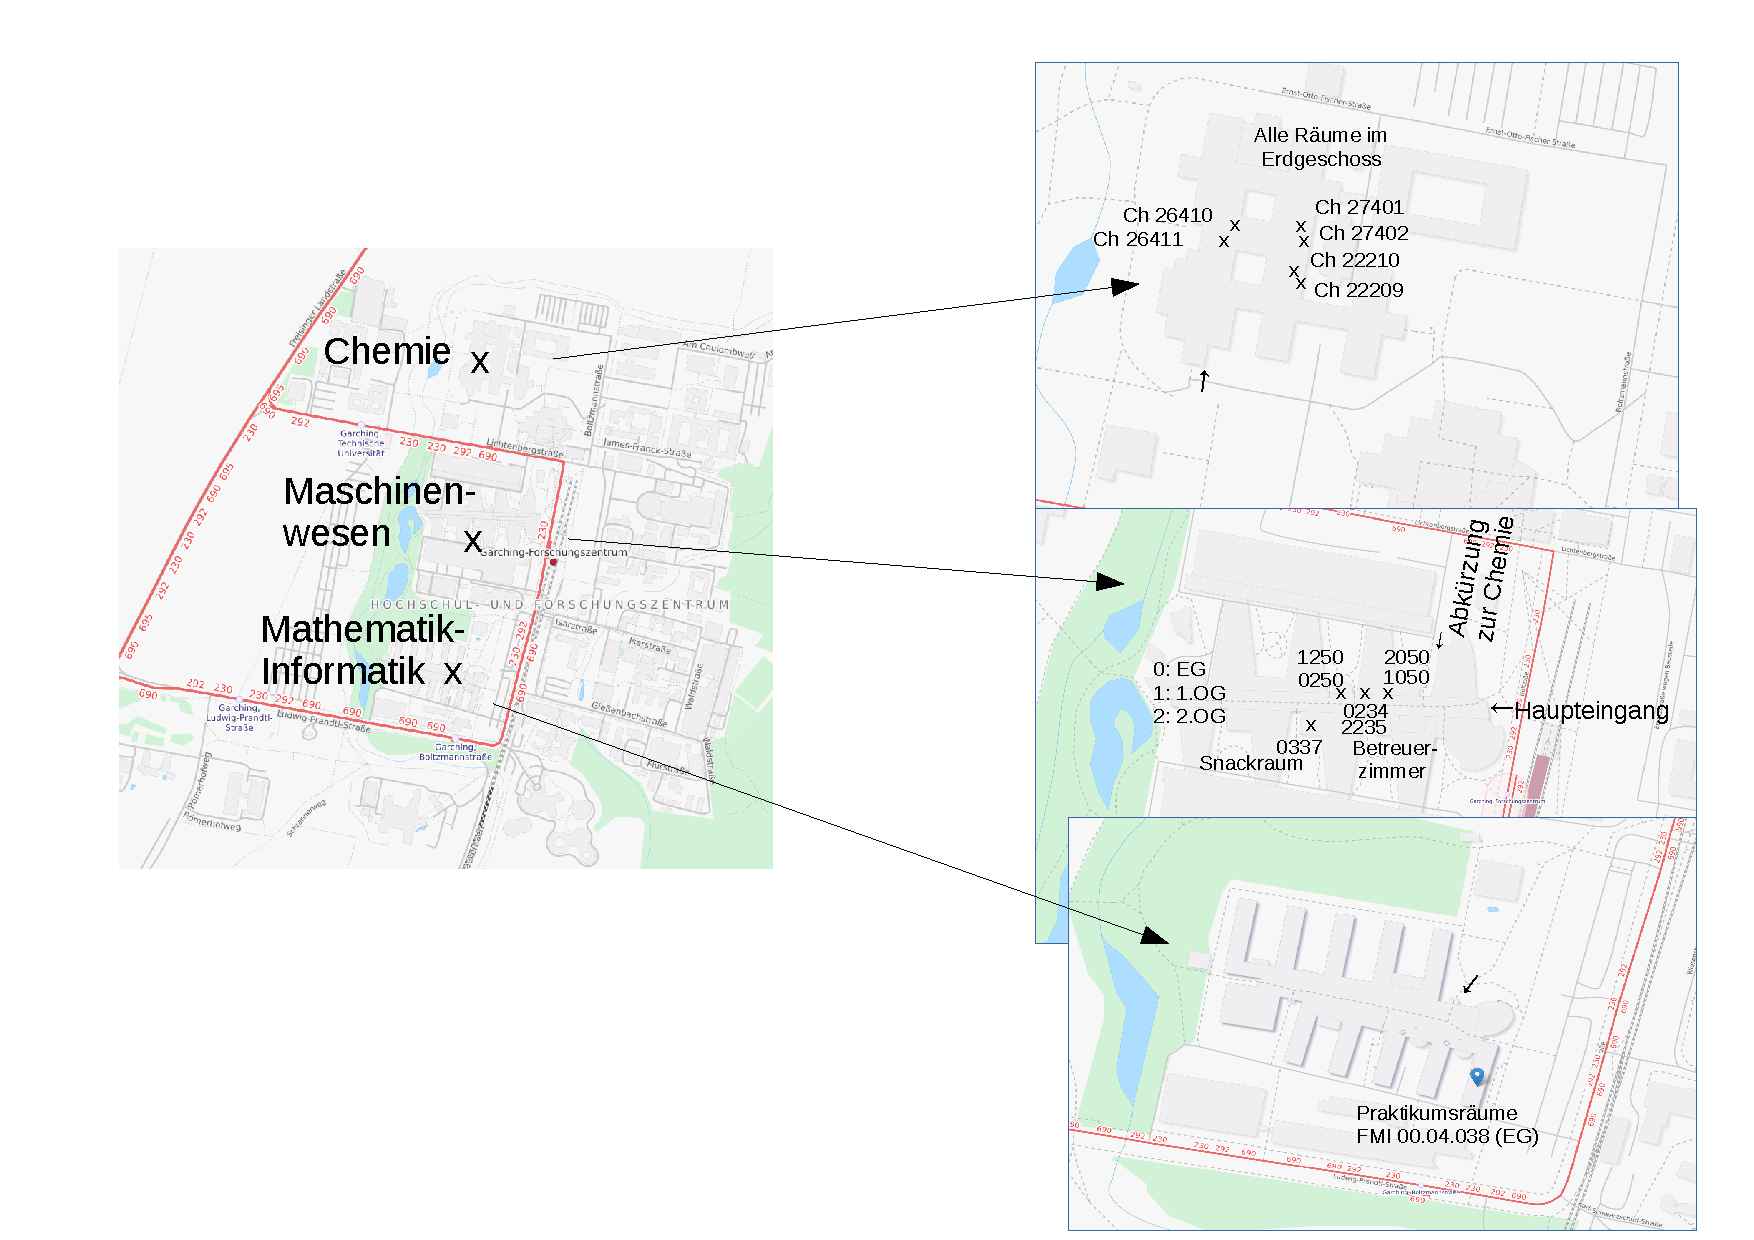
\includegraphics[scale=0.5]{campus_map.pdf}
\end{figure}
\newpage{}\begin{center}{\huge{}\textbf{Stundenplan von Jessica  Franz}}\end{center}\textbf{{\large{}Donnerstag}}\nopagebreak \\\begin{tabular} {|p{3cm} p{6cm} p{6cm}| }\hline \textbf{11:30 bis 13:45}&\textbf{Anreise zur TU München}&\textbf{Fakultät Maschinenwesen}\\\hline \textbf{12:00 bis 13:30}&\textbf{Mittagessen}&\textbf{Mensa Garching}\\\hline \textbf{14:00}&\textbf{Begrüßung}&\textbf{CH 26411}\\&Begrüßung, Besprechung des Zeitplans, Ausgabe der individuellen Stundenpläne,...&\\\hline \textbf{14:50 bis 16:20}&\textbf{Elektrische Schaltungen}&\textbf{MW 0250}\\&Betreuer: Christopher Pfeiffer&ca. 16 Teilnehmer\\\hline \textbf{16:40 bis 18:10}&\textbf{Himmelsmechanik}&\textbf{MW 2050}\\&Betreuer: Lars Dehlwes&ca. 19 Teilnehmer\\\hline \textbf{18:30}&\textbf{Fahrt zur Jugendherberge}&\textbf{}\\\hline \textbf{19:00}&\textbf{Abendessen}&\textbf{Jugendherberge}\\\hline \end{tabular}\\\vspace{5.00000mm}~\\\textbf{{\large{}Freitag}}\nopagebreak \\\begin{tabular} {|p{3cm} p{6cm} p{6cm}| }\hline \textbf{06:30 bis 09:00}&\textbf{Frühstück}&\textbf{Jugendherberge}\\\hline \textbf{09:00 bis 13:00}&frei&\\\hline \textbf{13:00 bis 14:00}&\textbf{Mittagessen}&\textbf{Mensa Garching}\\\hline \textbf{14:20 bis 15:50}&\textbf{Gewöhnliche Differentialgleichungen}&\textbf{MW 1250}\\&Betreuer: Sven Jandura&ca. 20 Teilnehmer\\\hline \textbf{16:10 bis 17:40}&\textbf{Näherungsmethoden}&\textbf{CH 26410}\\&Betreuer: Vincent Grande&ca. 11 Teilnehmer\\\hline \textbf{18:00 bis 18:20}&\textbf{Erlebnisbericht IPhO}&\textbf{CH 26411}\\\hline \textbf{18:30}&\textbf{Fahrt zur Jugendherberge}&\textbf{}\\\hline \textbf{19:00}&\textbf{Abendessen}&\textbf{Jugendherberge}\\\hline \end{tabular}\\\vspace{5.00000mm}~\\\textbf{{\large{}Samstag}}\nopagebreak \\\begin{tabular} {|p{3cm} p{6cm} p{6cm}| }\hline \textbf{06:30 bis 08:00}&\textbf{Frühstück}&\textbf{Jugendherberge}\\\hline \textbf{08:00}&\textbf{Fahrt zur TU}&\textbf{}\\\hline \textbf{09:00 bis 10:30}&\textbf{Experimentieren und Auswerten}&\textbf{CH 26411}\\&Betreuer: Ann-Kathrin Raab&ca. 18 Teilnehmer\\\hline \textbf{10:50 bis 12:20}&\textbf{Quanten- und Atomphysik I}&\textbf{MW 2050}\\&Betreuer: Vitaly Andreev&ca. 13 Teilnehmer\\\hline \textbf{12:40 bis 14:00}&\textbf{Mittagessen}&\textbf{Fakultät Maschinenwesen}\\\hline \textbf{14:20 bis 15:50}&\textbf{Thermodynamik 1}&\textbf{MW 1250}\\&Betreuer: Maximilian Marienhagen&ca. 9 Teilnehmer\\\hline \textbf{16:10 bis 17:40}&\textbf{Wellenoptik}&\textbf{CH 26410}\\&Betreuer: Christopher Pfeiffer&ca. 7 Teilnehmer\\\hline \textbf{18:00 bis 18:20}&\textbf{Vorstellung GYPT}&\textbf{CH 26411}\\\hline \textbf{18:30}&\textbf{Fahrt zur Jugendherberge}&\textbf{}\\\hline \textbf{19:00}&\textbf{Abendessen}&\textbf{Jugendherberge}\\\hline \end{tabular}\\\vspace{5.00000mm}~\\\textbf{{\large{}Sonntag}}\nopagebreak \\\begin{tabular} {|p{3cm} p{6cm} p{6cm}| }\hline \textbf{06:30 bis 08:00}&\textbf{Frühstück}&\textbf{Jugendherberge}\\\hline \textbf{08:00}&\textbf{Fahrt zur TU}&\textbf{}\\\hline \textbf{09:00 bis 10:30}&\textbf{Spezielle Relativitätstheorie}&\textbf{MW 0250}\\&Betreuer: Johannes Rothe&ca. 12 Teilnehmer\\\hline \textbf{10:50 bis 12:20}&\textbf{Relativistische Teilchenphysik}&\textbf{CH 22210}\\&Betreuer: Lars Dehlwes&ca. 11 Teilnehmer\\\hline \textbf{12:40 bis 13:00}&\textbf{Verabschiedung}&\textbf{CH 26411}\\\hline \textbf{13:00}&\textbf{Individuelle Abreise}&\textbf{}\\\hline \textbf{13:00 bis 14:00}&\textbf{Mittagessen}&\textbf{}\\\hline \end{tabular}\\\vspace{5.00000mm}~\\
Notfallnummern: \\
Sven Jandura: xxxx xxxxxxxxx \\
Johannes Rothe: xxxx xxxxxxxxx \\

\large Hast du Lust, die Andern vom Seminar wiederzusehen?\\
\normalsize Dann komm doch einfach zum \textbf{Vereinstreffen}. Dazu musst du kein Vereinsmitglied sein. Neben interesannten Vorträgen und Exkursionen sind jede Menge Spiel und Spaß geplant. Schau in einem Monat einfach noch mal auf der Website vorbei. Wir freuen uns, wenn du dabei bist.

\begin{figure}[!h]
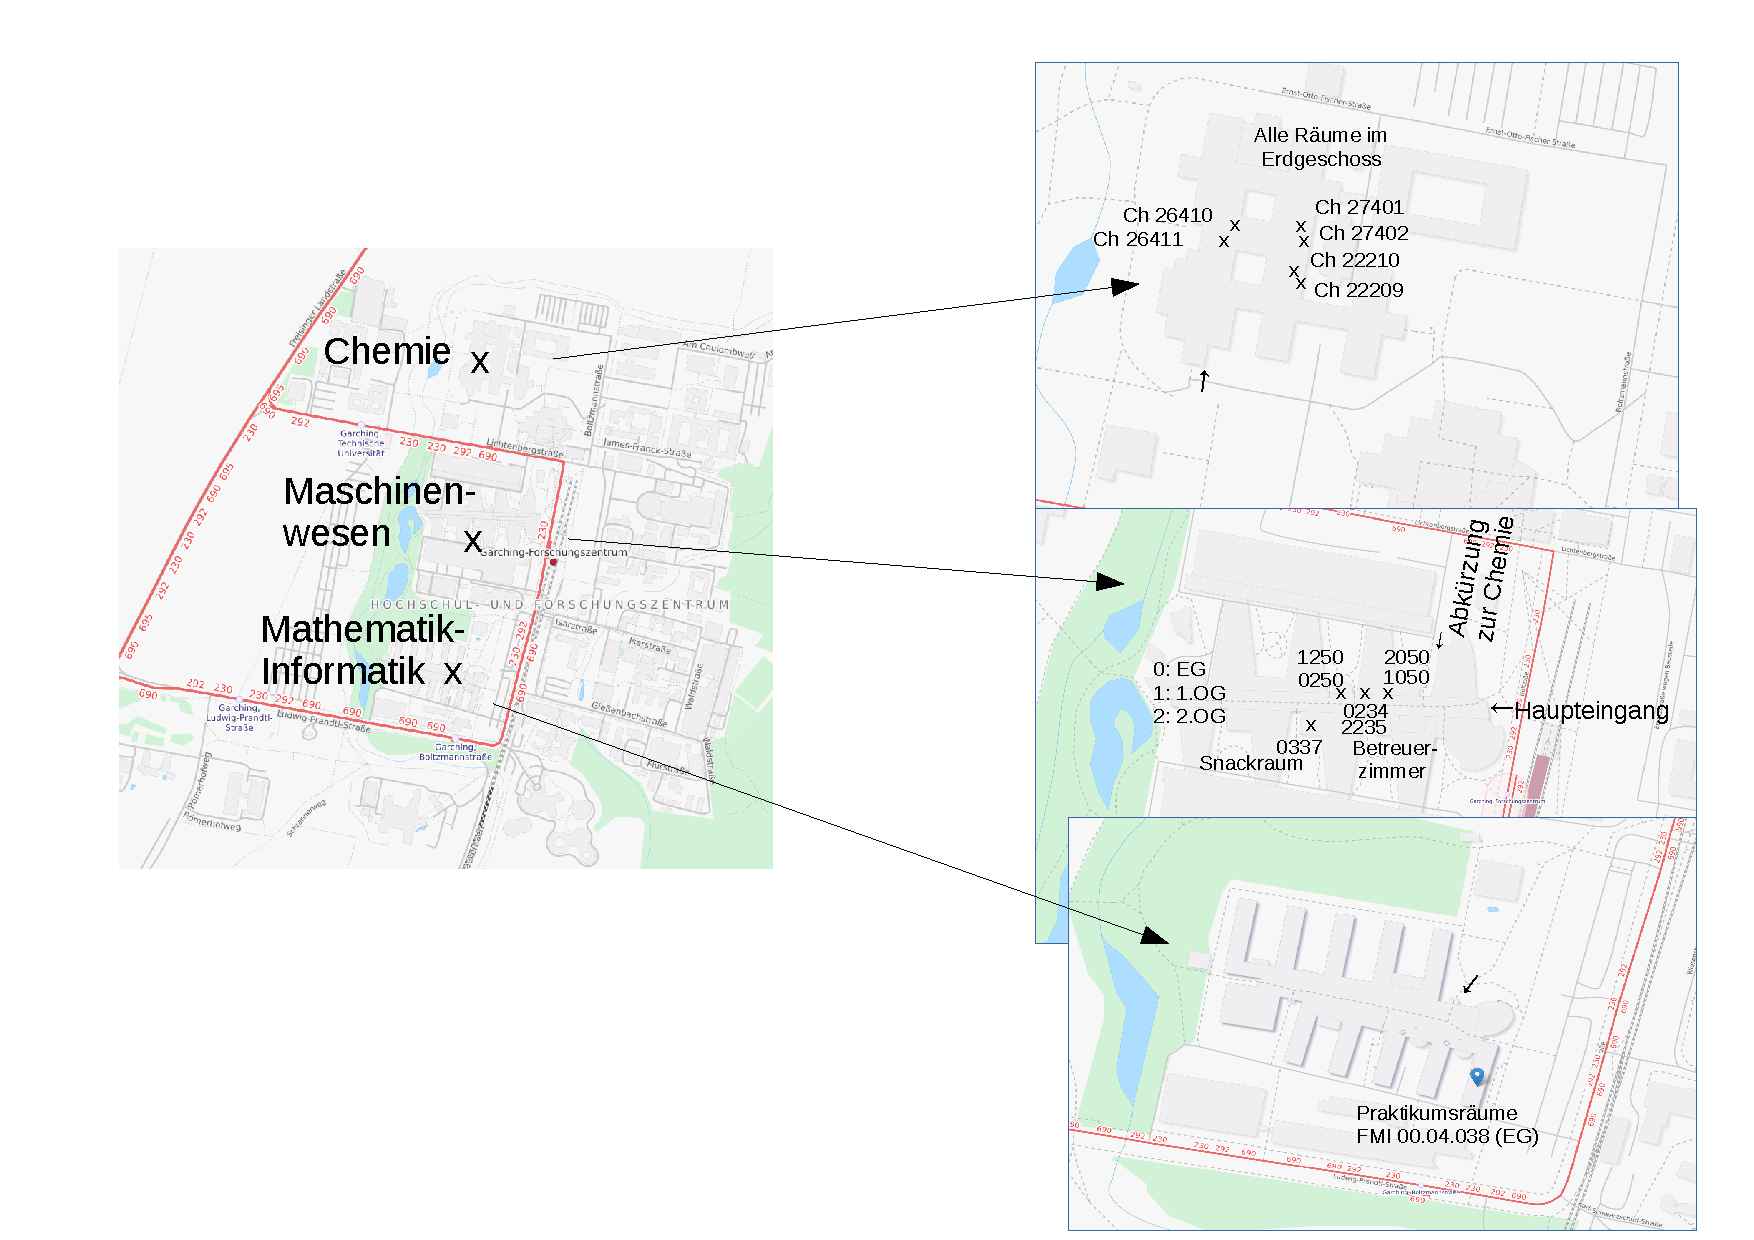
\includegraphics[scale=0.5]{campus_map.pdf}
\end{figure}
\newpage{}\begin{center}{\huge{}\textbf{Stundenplan von Johannes Fleischer}}\end{center}\textbf{{\large{}Donnerstag}}\nopagebreak \\\begin{tabular} {|p{3cm} p{6cm} p{6cm}| }\hline \textbf{11:30 bis 13:45}&\textbf{Anreise zur TU München}&\textbf{Fakultät Maschinenwesen}\\\hline \textbf{12:00 bis 13:30}&\textbf{Mittagessen}&\textbf{Mensa Garching}\\\hline \textbf{14:00}&\textbf{Begrüßung}&\textbf{CH 26411}\\&Begrüßung, Besprechung des Zeitplans, Ausgabe der individuellen Stundenpläne,...&\\\hline \textbf{14:50 bis 16:20}&\textbf{Quanten- und Atomphysik I}&\textbf{CH 26410}\\&Betreuer: Ismail Achmed-Zade&ca. 28 Teilnehmer\\\hline \textbf{16:40 bis 18:10}&\textbf{Klassische Mechanik}&\textbf{MW 1250}\\&Betreuer: Maximilian Marienhagen&ca. 10 Teilnehmer\\\hline \textbf{18:30}&\textbf{Fahrt zur Jugendherberge}&\textbf{}\\\hline \textbf{19:00}&\textbf{Abendessen}&\textbf{Jugendherberge}\\\hline \end{tabular}\\\vspace{5.00000mm}~\\\textbf{{\large{}Freitag}}\nopagebreak \\\begin{tabular} {|p{3cm} p{6cm} p{6cm}| }\hline \textbf{06:30 bis 09:00}&\textbf{Frühstück}&\textbf{Jugendherberge}\\\hline \textbf{09:00 bis 13:00}&frei&\\\hline \textbf{13:00 bis 14:00}&\textbf{Mittagessen}&\textbf{Mensa Garching}\\\hline \textbf{14:20 bis 15:50}&\textbf{Rotationsbewegungen}&\textbf{MW 1050}\\&Betreuer: Vincent Grande&ca. 6 Teilnehmer\\\hline \textbf{16:10 bis 17:40}&\textbf{Spezielle Relativitätstheorie}&\textbf{MW 1250}\\&Betreuer: Johannes Rothe&ca. 19 Teilnehmer\\\hline \textbf{18:00 bis 18:20}&\textbf{Erlebnisbericht IPhO}&\textbf{CH 26411}\\\hline \textbf{18:30}&\textbf{Fahrt zur Jugendherberge}&\textbf{}\\\hline \textbf{19:00}&\textbf{Abendessen}&\textbf{Jugendherberge}\\\hline \end{tabular}\\\vspace{5.00000mm}~\\\textbf{{\large{}Samstag}}\nopagebreak \\\begin{tabular} {|p{3cm} p{6cm} p{6cm}| }\hline \textbf{06:30 bis 08:00}&\textbf{Frühstück}&\textbf{Jugendherberge}\\\hline \textbf{08:00}&\textbf{Fahrt zur TU}&\textbf{}\\\hline \textbf{09:00 bis 10:30}&\textbf{Thermodynamik 2 - Statistische Physik}&\textbf{MW 1050}\\&Betreuer: Vitaly Andreev&ca. 17 Teilnehmer\\\hline \textbf{10:50 bis 12:20}&\textbf{Experiment Pohlsches Rad}&\textbf{Praktikum Pohlsches Rad}\\&Betreuer: Eugen Dizer&ca. 4 Teilnehmer\\\hline \textbf{12:40 bis 14:00}&\textbf{Mittagessen}&\textbf{Fakultät Maschinenwesen}\\\hline \textbf{14:20 bis 15:50}&\textbf{Relativistische Teilchenphysik}&\textbf{CH 22210}\\&Betreuer: Lars Dehlwes&ca. 23 Teilnehmer\\\hline \textbf{16:10 bis 17:40}&\textbf{Quanten- und Atomphysik II}&\textbf{CH 22209}\\&Betreuer: Vitaly Andreev&ca. 28 Teilnehmer\\\hline \textbf{18:00 bis 18:20}&\textbf{Vorstellung GYPT}&\textbf{CH 26411}\\\hline \textbf{18:30}&\textbf{Fahrt zur Jugendherberge}&\textbf{}\\\hline \textbf{19:00}&\textbf{Abendessen}&\textbf{Jugendherberge}\\\hline \end{tabular}\\\vspace{5.00000mm}~\\\textbf{{\large{}Sonntag}}\nopagebreak \\\begin{tabular} {|p{3cm} p{6cm} p{6cm}| }\hline \textbf{06:30 bis 08:00}&\textbf{Frühstück}&\textbf{Jugendherberge}\\\hline \textbf{08:00}&\textbf{Fahrt zur TU}&\textbf{}\\\hline \textbf{09:00 bis 10:30}&\textbf{Theoretische Mechanik}&\textbf{CH 22210}\\&Betreuer: Eugen Dizer&ca. 13 Teilnehmer\\\hline \textbf{10:50 bis 12:20}&\textbf{Aufgabenseminar Quanten- und Atomphysik und Struktur der Materie}&\textbf{MW 1250}\\&Betreuer: Vitaly Andreev&ca. 24 Teilnehmer\\\hline \textbf{12:40 bis 13:00}&\textbf{Verabschiedung}&\textbf{CH 26411}\\\hline \textbf{13:00}&\textbf{Individuelle Abreise}&\textbf{}\\\hline \textbf{13:00 bis 14:00}&\textbf{Mittagessen}&\textbf{}\\\hline \end{tabular}\\\vspace{5.00000mm}~\\
Notfallnummern: \\
Sven Jandura: xxxx xxxxxxxxx \\
Johannes Rothe: xxxx xxxxxxxxx \\

\large Hast du Lust, die Andern vom Seminar wiederzusehen?\\
\normalsize Dann komm doch einfach zum \textbf{Vereinstreffen}. Dazu musst du kein Vereinsmitglied sein. Neben interesannten Vorträgen und Exkursionen sind jede Menge Spiel und Spaß geplant. Schau in einem Monat einfach noch mal auf der Website vorbei. Wir freuen uns, wenn du dabei bist.

\begin{figure}[!h]
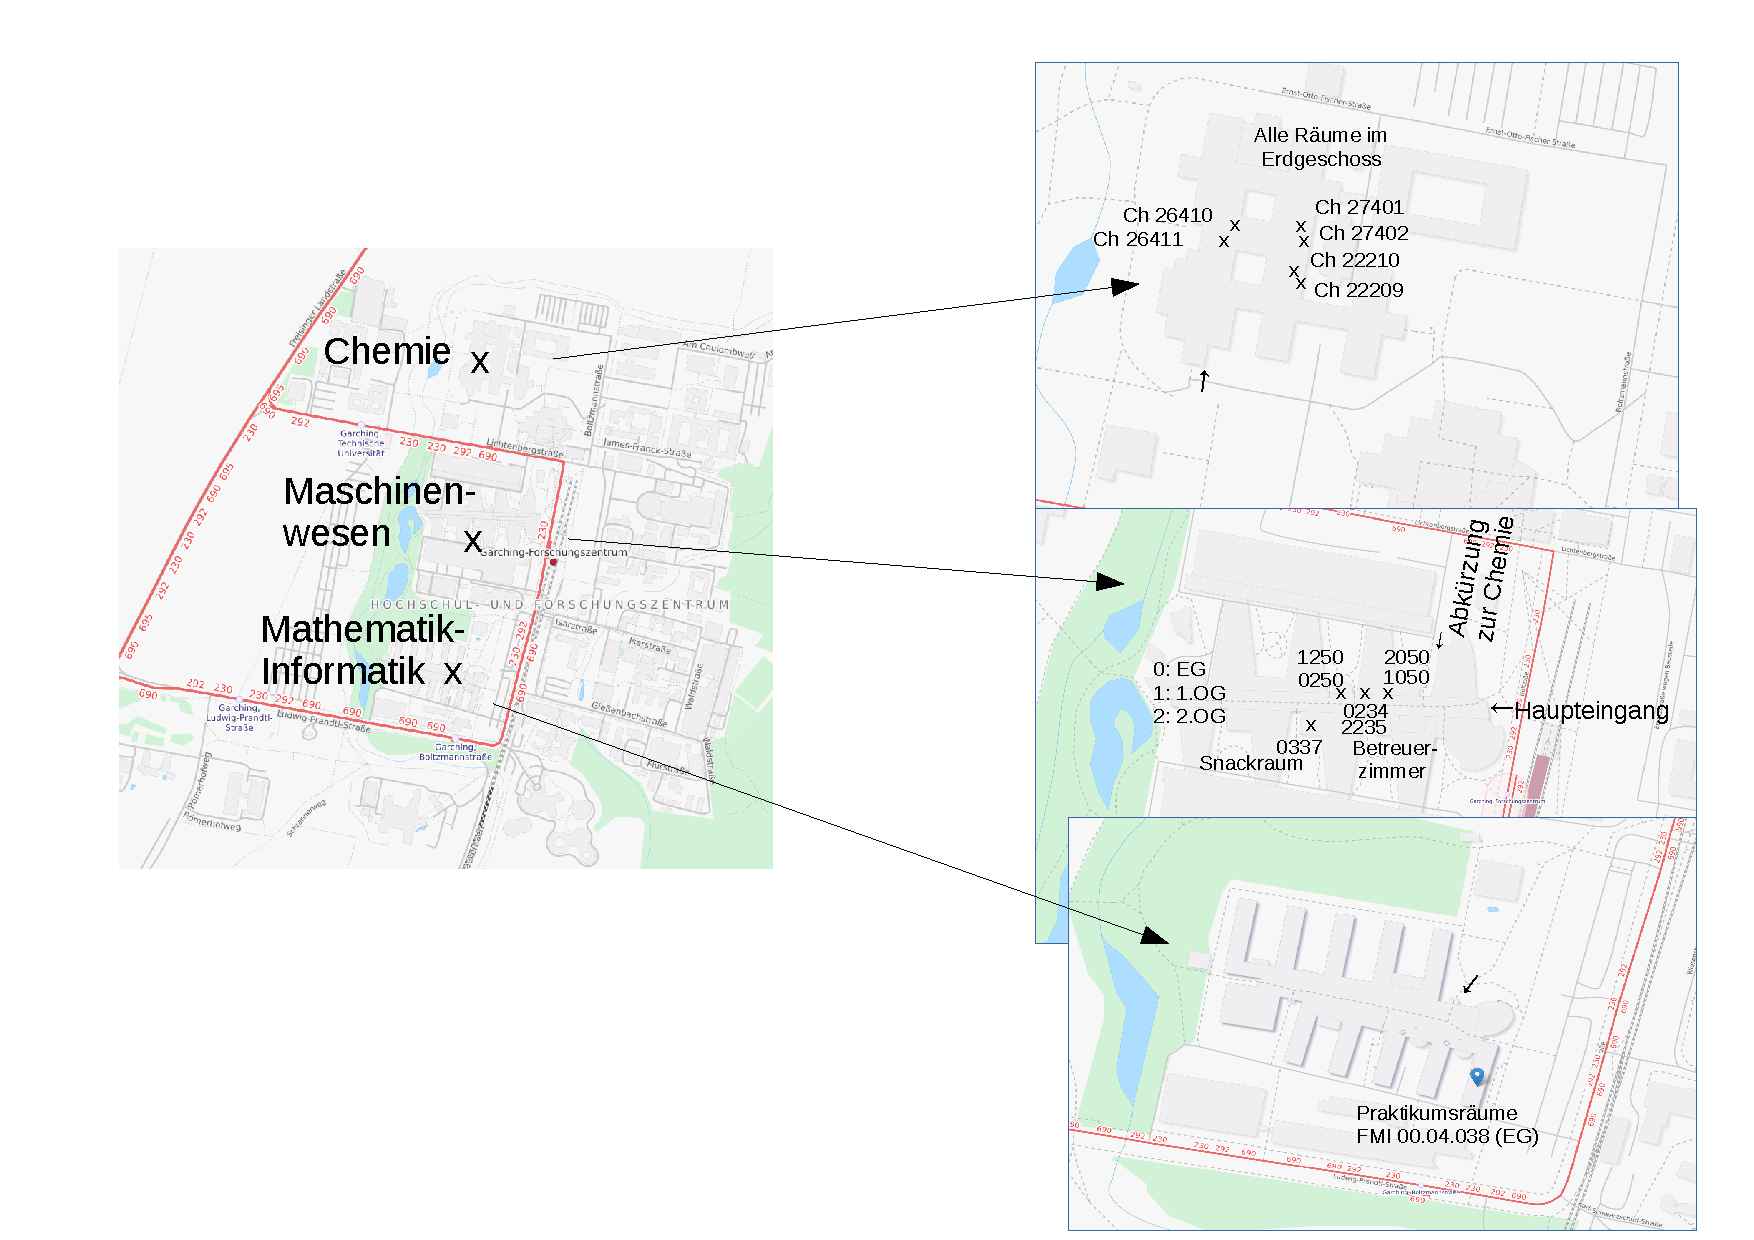
\includegraphics[scale=0.5]{campus_map.pdf}
\end{figure}
\newpage{}\begin{center}{\huge{}\textbf{Stundenplan von Jonas Götzfried}}\end{center}\textbf{{\large{}Donnerstag}}\nopagebreak \\\begin{tabular} {|p{3cm} p{6cm} p{6cm}| }\hline \textbf{11:30 bis 13:45}&\textbf{Anreise zur TU München}&\textbf{Fakultät Maschinenwesen}\\\hline \textbf{12:00 bis 13:30}&\textbf{Mittagessen}&\textbf{Mensa Garching}\\\hline \textbf{14:00}&\textbf{Begrüßung}&\textbf{CH 26411}\\&Begrüßung, Besprechung des Zeitplans, Ausgabe der individuellen Stundenpläne,...&\\\hline \textbf{14:50 bis 16:20}&\textbf{Quanten- und Atomphysik I}&\textbf{CH 26410}\\&Betreuer: Ismail Achmed-Zade&ca. 28 Teilnehmer\\\hline \textbf{16:40 bis 18:10}&\textbf{Geometrische Optik}&\textbf{MW 0250}\\&Betreuer: Christopher Pfeiffer&ca. 13 Teilnehmer\\\hline \textbf{18:30}&\textbf{Fahrt zur Jugendherberge}&\textbf{}\\\hline \textbf{19:00}&\textbf{Abendessen}&\textbf{Jugendherberge}\\\hline \end{tabular}\\\vspace{5.00000mm}~\\\textbf{{\large{}Freitag}}\nopagebreak \\\begin{tabular} {|p{3cm} p{6cm} p{6cm}| }\hline \textbf{06:30 bis 09:00}&\textbf{Frühstück}&\textbf{Jugendherberge}\\\hline \textbf{09:00 bis 13:00}&frei&\\\hline \textbf{13:00 bis 14:00}&\textbf{Mittagessen}&\textbf{Mensa Garching}\\\hline \textbf{14:20 bis 15:50}&\textbf{Kernphysik}&\textbf{MW 0250}\\&Betreuer: Johannes Rothe&ca. 18 Teilnehmer\\\hline \textbf{16:10 bis 17:40}&\textbf{Komplexe Wechselstromrechnung}&\textbf{MW 1050}\\&Betreuer: Vincent Grande&ca. 8 Teilnehmer\\\hline \textbf{18:00 bis 18:20}&\textbf{Erlebnisbericht IPhO}&\textbf{CH 26411}\\\hline \textbf{18:30}&\textbf{Fahrt zur Jugendherberge}&\textbf{}\\\hline \textbf{19:00}&\textbf{Abendessen}&\textbf{Jugendherberge}\\\hline \end{tabular}\\\vspace{5.00000mm}~\\\textbf{{\large{}Samstag}}\nopagebreak \\\begin{tabular} {|p{3cm} p{6cm} p{6cm}| }\hline \textbf{06:30 bis 08:00}&\textbf{Frühstück}&\textbf{Jugendherberge}\\\hline \textbf{08:00}&\textbf{Fahrt zur TU}&\textbf{}\\\hline \textbf{09:00 bis 10:30}&\textbf{Aufgabenseminar klassische Mechanik}&\textbf{MW 0234}\\&Betreuer: Maximilian Marienhagen&ca. 5 Teilnehmer\\\hline \textbf{10:50 bis 12:20}&\textbf{Experiment Brennstoffzelle}&\textbf{Praktikum Brennstoffzelle}\\&Betreuer: Aaron Wild&ca. 6 Teilnehmer\\\hline \textbf{12:40 bis 14:00}&\textbf{Mittagessen}&\textbf{Fakultät Maschinenwesen}\\\hline \textbf{14:20 bis 15:50}&\textbf{Relativistische Teilchenphysik}&\textbf{CH 22210}\\&Betreuer: Lars Dehlwes&ca. 23 Teilnehmer\\\hline \textbf{16:10 bis 17:40}&\textbf{Quanten- und Atomphysik II}&\textbf{CH 22209}\\&Betreuer: Vitaly Andreev&ca. 28 Teilnehmer\\\hline \textbf{18:00 bis 18:20}&\textbf{Vorstellung GYPT}&\textbf{CH 26411}\\\hline \textbf{18:30}&\textbf{Fahrt zur Jugendherberge}&\textbf{}\\\hline \textbf{19:00}&\textbf{Abendessen}&\textbf{Jugendherberge}\\\hline \end{tabular}\\\vspace{5.00000mm}~\\\textbf{{\large{}Sonntag}}\nopagebreak \\\begin{tabular} {|p{3cm} p{6cm} p{6cm}| }\hline \textbf{06:30 bis 08:00}&\textbf{Frühstück}&\textbf{Jugendherberge}\\\hline \textbf{08:00}&\textbf{Fahrt zur TU}&\textbf{}\\\hline \textbf{09:00 bis 10:30}&\textbf{Theoretische Mechanik}&\textbf{CH 22210}\\&Betreuer: Eugen Dizer&ca. 13 Teilnehmer\\\hline \textbf{10:50 bis 12:20}&\textbf{Aufgabenseminar Quanten- und Atomphysik und Struktur der Materie}&\textbf{MW 1250}\\&Betreuer: Vitaly Andreev&ca. 24 Teilnehmer\\\hline \textbf{12:40 bis 13:00}&\textbf{Verabschiedung}&\textbf{CH 26411}\\\hline \textbf{13:00}&\textbf{Individuelle Abreise}&\textbf{}\\\hline \textbf{13:00 bis 14:00}&\textbf{Mittagessen}&\textbf{}\\\hline \end{tabular}\\\vspace{5.00000mm}~\\
Notfallnummern: \\
Sven Jandura: xxxx xxxxxxxxx \\
Johannes Rothe: xxxx xxxxxxxxx \\

\large Hast du Lust, die Andern vom Seminar wiederzusehen?\\
\normalsize Dann komm doch einfach zum \textbf{Vereinstreffen}. Dazu musst du kein Vereinsmitglied sein. Neben interesannten Vorträgen und Exkursionen sind jede Menge Spiel und Spaß geplant. Schau in einem Monat einfach noch mal auf der Website vorbei. Wir freuen uns, wenn du dabei bist.

\begin{figure}[!h]
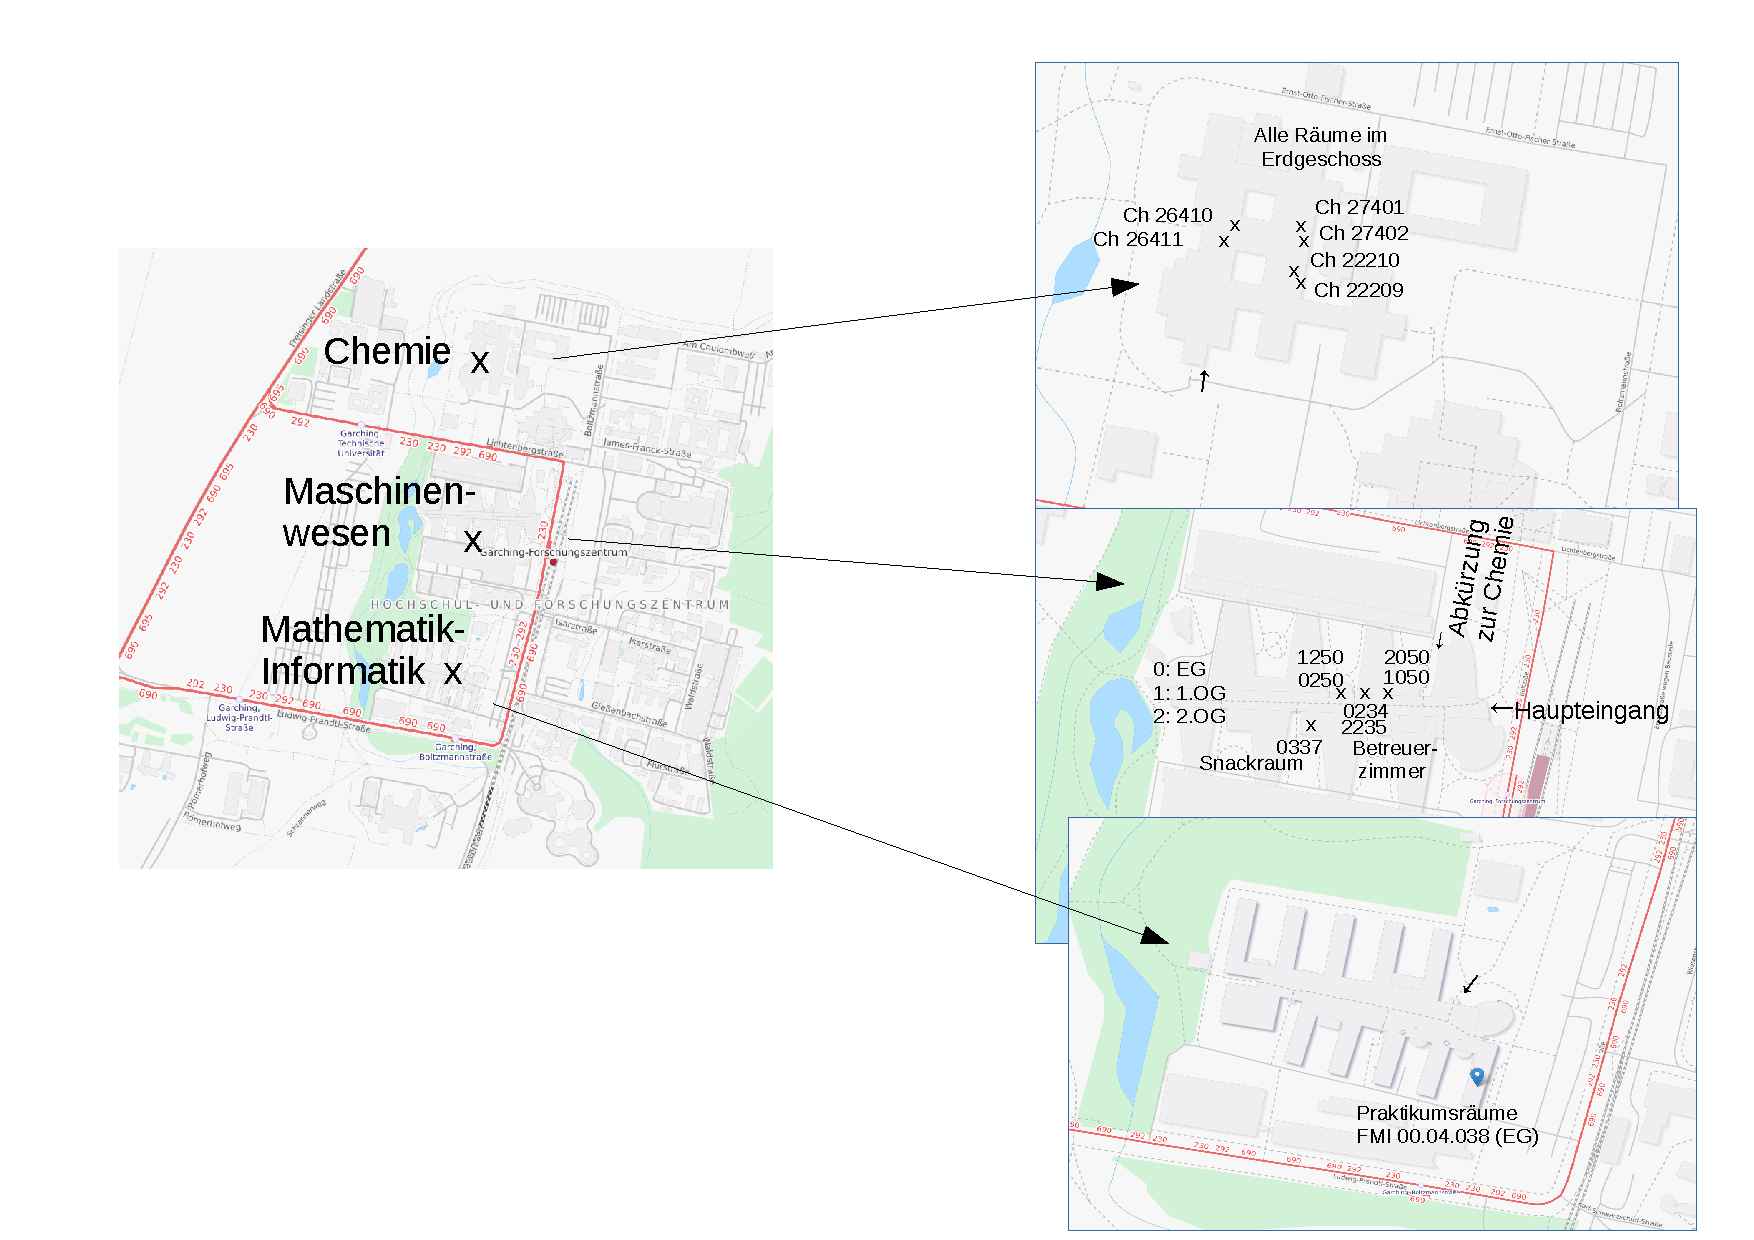
\includegraphics[scale=0.5]{campus_map.pdf}
\end{figure}
\newpage{}\begin{center}{\huge{}\textbf{Stundenplan von Josephine Dabrunz}}\end{center}\textbf{{\large{}Donnerstag}}\nopagebreak \\\begin{tabular} {|p{3cm} p{6cm} p{6cm}| }\hline \textbf{11:30 bis 13:45}&\textbf{Anreise zur TU München}&\textbf{Fakultät Maschinenwesen}\\\hline \textbf{12:00 bis 13:30}&\textbf{Mittagessen}&\textbf{Mensa Garching}\\\hline \textbf{14:00}&\textbf{Begrüßung}&\textbf{CH 26411}\\&Begrüßung, Besprechung des Zeitplans, Ausgabe der individuellen Stundenpläne,...&\\\hline \textbf{14:50 bis 16:20}&\textbf{Quanten- und Atomphysik I}&\textbf{CH 26410}\\&Betreuer: Ismail Achmed-Zade&ca. 28 Teilnehmer\\\hline \textbf{16:40 bis 18:10}&\textbf{Einführung ins Integrieren}&\textbf{MW 1050}\\&Betreuer: Johannes Rothe&ca. 14 Teilnehmer\\\hline \textbf{18:30}&\textbf{Fahrt zur Jugendherberge}&\textbf{}\\\hline \textbf{19:00}&\textbf{Abendessen}&\textbf{Jugendherberge}\\\hline \end{tabular}\\\vspace{5.00000mm}~\\\textbf{{\large{}Freitag}}\nopagebreak \\\begin{tabular} {|p{3cm} p{6cm} p{6cm}| }\hline \textbf{06:30 bis 09:00}&\textbf{Frühstück}&\textbf{Jugendherberge}\\\hline \textbf{09:00 bis 13:00}&frei&\\\hline \textbf{13:00 bis 14:00}&\textbf{Mittagessen}&\textbf{Mensa Garching}\\\hline \textbf{14:20 bis 15:50}&\textbf{Experiment spezifische Elektronenladung}&\textbf{Praktikum spezifische Elektronenladung}\\&Betreuer: Felix Wechsler&ca. 6 Teilnehmer\\\hline \textbf{16:10 bis 17:40}&\textbf{Komplexe Wechselstromrechnung}&\textbf{MW 1050}\\&Betreuer: Vincent Grande&ca. 8 Teilnehmer\\\hline \textbf{18:00 bis 18:20}&\textbf{Erlebnisbericht IPhO}&\textbf{CH 26411}\\\hline \textbf{18:30}&\textbf{Fahrt zur Jugendherberge}&\textbf{}\\\hline \textbf{19:00}&\textbf{Abendessen}&\textbf{Jugendherberge}\\\hline \end{tabular}\\\vspace{5.00000mm}~\\\textbf{{\large{}Samstag}}\nopagebreak \\\begin{tabular} {|p{3cm} p{6cm} p{6cm}| }\hline \textbf{06:30 bis 08:00}&\textbf{Frühstück}&\textbf{Jugendherberge}\\\hline \textbf{08:00}&\textbf{Fahrt zur TU}&\textbf{}\\\hline \textbf{09:00 bis 10:30}&\textbf{Experimentieren und Auswerten}&\textbf{CH 26411}\\&Betreuer: Ann-Kathrin Raab&ca. 18 Teilnehmer\\\hline \textbf{10:50 bis 12:20}&\textbf{Spezielle Relativitätstheorie}&\textbf{MW 0250}\\&Betreuer: Johannes Rothe&ca. 12 Teilnehmer\\\hline \textbf{12:40 bis 14:00}&\textbf{Mittagessen}&\textbf{Fakultät Maschinenwesen}\\\hline \textbf{14:20 bis 15:50}&\textbf{Rotationsbewegungen}&\textbf{MW 0250}\\&Betreuer: Vincent Grande&ca. 3 Teilnehmer\\\hline \textbf{16:10 bis 17:40}&\textbf{Himmelsmechanik}&\textbf{CH 22210}\\&Betreuer: Lars Dehlwes&ca. 10 Teilnehmer\\\hline \textbf{18:00 bis 18:20}&\textbf{Vorstellung GYPT}&\textbf{CH 26411}\\\hline \textbf{18:30}&\textbf{Fahrt zur Jugendherberge}&\textbf{}\\\hline \textbf{19:00}&\textbf{Abendessen}&\textbf{Jugendherberge}\\\hline \end{tabular}\\\vspace{5.00000mm}~\\\textbf{{\large{}Sonntag}}\nopagebreak \\\begin{tabular} {|p{3cm} p{6cm} p{6cm}| }\hline \textbf{06:30 bis 08:00}&\textbf{Frühstück}&\textbf{Jugendherberge}\\\hline \textbf{08:00}&\textbf{Fahrt zur TU}&\textbf{}\\\hline \textbf{09:00 bis 10:30}&\textbf{Theoretische Mechanik}&\textbf{CH 22210}\\&Betreuer: Eugen Dizer&ca. 13 Teilnehmer\\\hline \textbf{10:50 bis 12:20}&\textbf{Elektrische Blackboxen}&\textbf{Praktikum Blackboxen}\\&Betreuer: Eugen Dizer&ca. 6 Teilnehmer\\\hline \textbf{12:40 bis 13:00}&\textbf{Verabschiedung}&\textbf{CH 26411}\\\hline \textbf{13:00}&\textbf{Individuelle Abreise}&\textbf{}\\\hline \textbf{13:00 bis 14:00}&\textbf{Mittagessen}&\textbf{}\\\hline \end{tabular}\\\vspace{5.00000mm}~\\
Notfallnummern: \\
Sven Jandura: xxxx xxxxxxxxx \\
Johannes Rothe: xxxx xxxxxxxxx \\

\large Hast du Lust, die Andern vom Seminar wiederzusehen?\\
\normalsize Dann komm doch einfach zum \textbf{Vereinstreffen}. Dazu musst du kein Vereinsmitglied sein. Neben interesannten Vorträgen und Exkursionen sind jede Menge Spiel und Spaß geplant. Schau in einem Monat einfach noch mal auf der Website vorbei. Wir freuen uns, wenn du dabei bist.

\begin{figure}[!h]
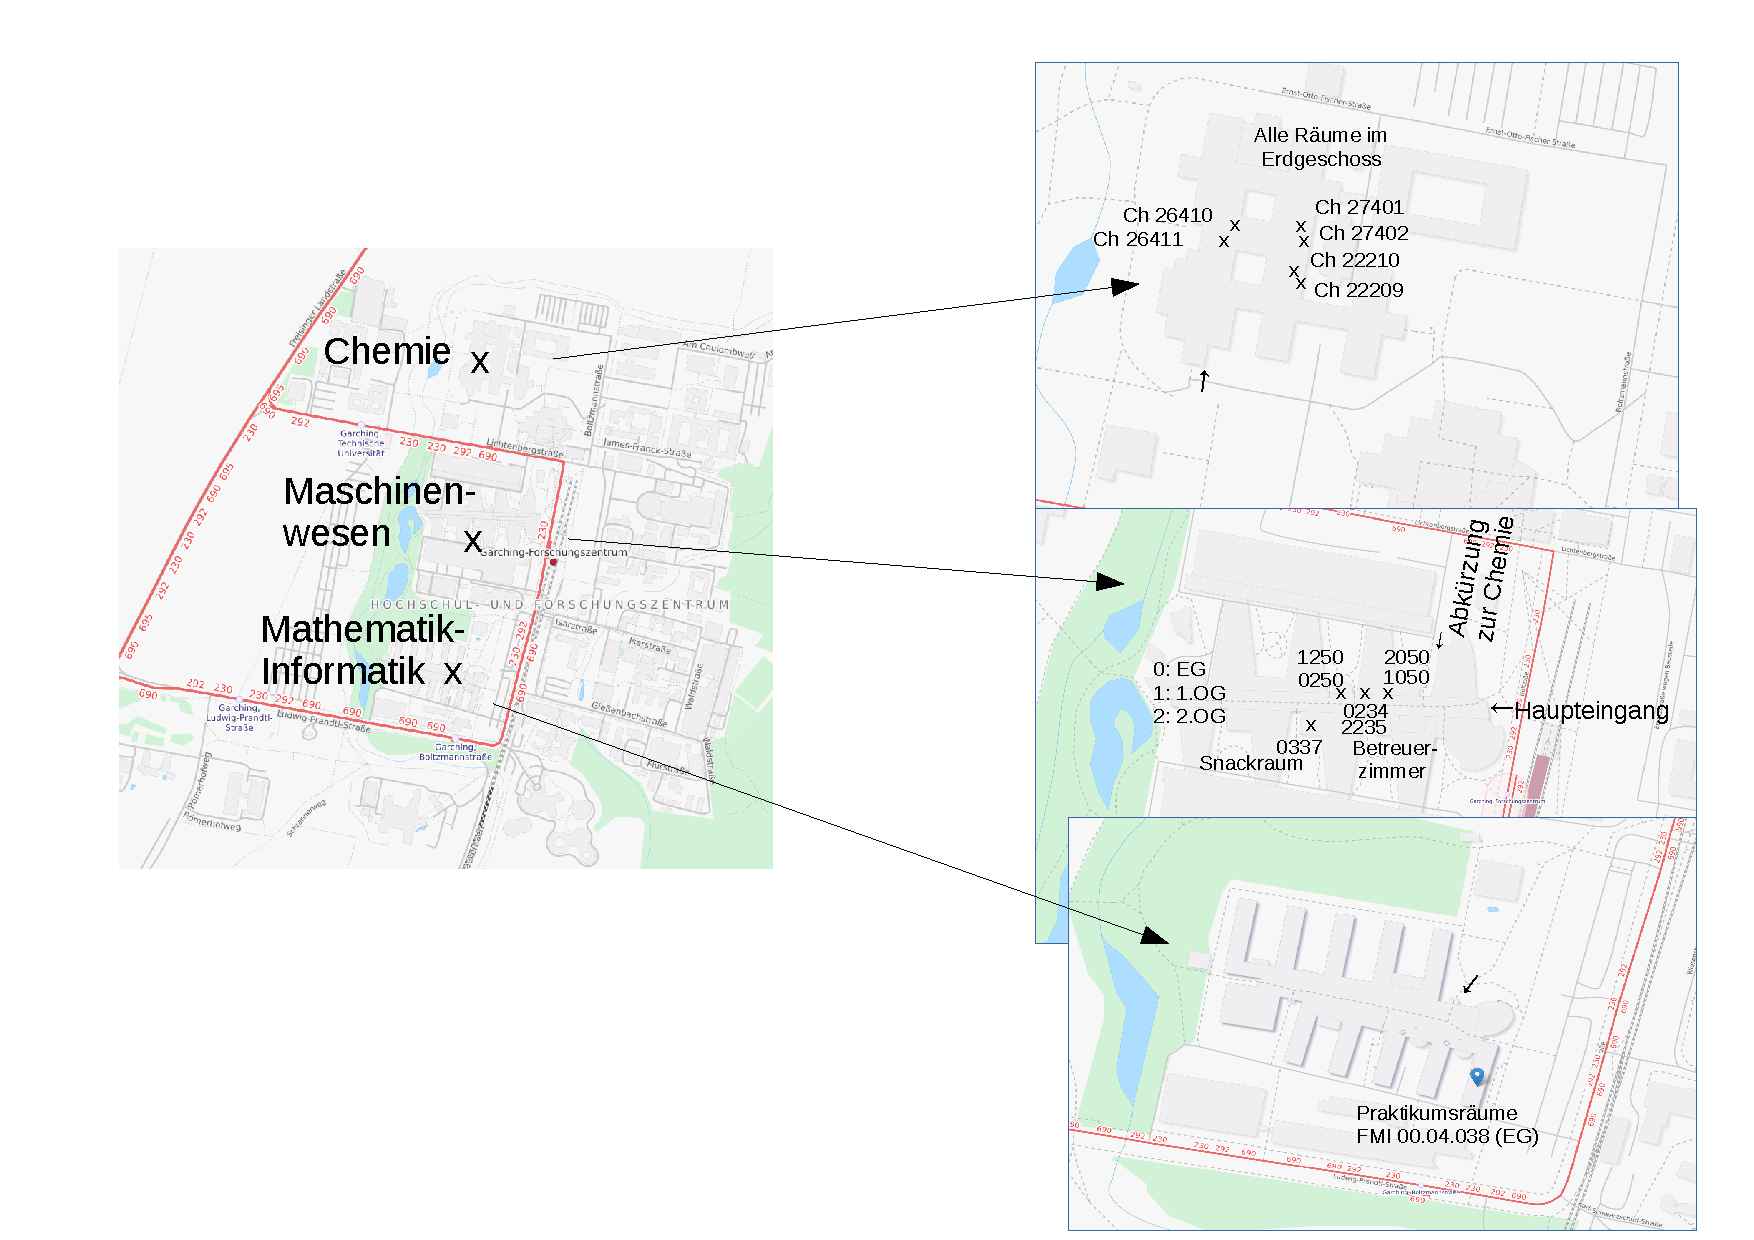
\includegraphics[scale=0.5]{campus_map.pdf}
\end{figure}
\newpage{}\begin{center}{\huge{}\textbf{Stundenplan von Karim Alaa El-Din}}\end{center}\textbf{{\large{}Donnerstag}}\nopagebreak \\\begin{tabular} {|p{3cm} p{6cm} p{6cm}| }\hline \textbf{11:30 bis 13:45}&\textbf{Anreise zur TU München}&\textbf{Fakultät Maschinenwesen}\\\hline \textbf{12:00 bis 13:30}&\textbf{Mittagessen}&\textbf{Mensa Garching}\\\hline \textbf{14:00}&\textbf{Begrüßung}&\textbf{CH 26411}\\&Begrüßung, Besprechung des Zeitplans, Ausgabe der individuellen Stundenpläne,...&\\\hline \textbf{14:50 bis 16:20}&\textbf{Thermodynamik 1}&\textbf{MW 1250}\\&Betreuer: Maximilian Marienhagen&ca. 12 Teilnehmer\\\hline \textbf{16:40 bis 18:10}&\textbf{Geometrische Optik}&\textbf{MW 0250}\\&Betreuer: Christopher Pfeiffer&ca. 13 Teilnehmer\\\hline \textbf{18:30}&\textbf{Fahrt zur Jugendherberge}&\textbf{}\\\hline \textbf{19:00}&\textbf{Abendessen}&\textbf{Jugendherberge}\\\hline \end{tabular}\\\vspace{5.00000mm}~\\\textbf{{\large{}Freitag}}\nopagebreak \\\begin{tabular} {|p{3cm} p{6cm} p{6cm}| }\hline \textbf{06:30 bis 09:00}&\textbf{Frühstück}&\textbf{Jugendherberge}\\\hline \textbf{09:00 bis 13:00}&\textbf{Besichtigung der Forschungsneutronenquelle FRM II}&\textbf{MW 2050}\\&Betreuer: Felix Wechsler&ca. 28 Teilnehmer\\\hline \textbf{13:00 bis 14:00}&\textbf{Mittagessen}&\textbf{Mensa Garching}\\\hline \textbf{14:20 bis 15:50}&\textbf{Aufgabenseminar Wärmelehre}&\textbf{MW 2050}\\&Betreuer: Maximilian Marienhagen&ca. 9 Teilnehmer\\\hline \textbf{16:10 bis 17:40}&\textbf{Näherungsmethoden}&\textbf{CH 26410}\\&Betreuer: Vincent Grande&ca. 11 Teilnehmer\\\hline \textbf{18:00 bis 18:20}&\textbf{Erlebnisbericht IPhO}&\textbf{CH 26411}\\\hline \textbf{18:30}&\textbf{Fahrt zur Jugendherberge}&\textbf{}\\\hline \textbf{19:00}&\textbf{Abendessen}&\textbf{Jugendherberge}\\\hline \end{tabular}\\\vspace{5.00000mm}~\\\textbf{{\large{}Samstag}}\nopagebreak \\\begin{tabular} {|p{3cm} p{6cm} p{6cm}| }\hline \textbf{06:30 bis 08:00}&\textbf{Frühstück}&\textbf{Jugendherberge}\\\hline \textbf{08:00}&\textbf{Fahrt zur TU}&\textbf{}\\\hline \textbf{09:00 bis 10:30}&\textbf{Thermodynamik 2 - Statistische Physik}&\textbf{MW 1050}\\&Betreuer: Vitaly Andreev&ca. 17 Teilnehmer\\\hline \textbf{10:50 bis 12:20}&\textbf{Quanten- und Atomphysik I}&\textbf{MW 2050}\\&Betreuer: Vitaly Andreev&ca. 13 Teilnehmer\\\hline \textbf{12:40 bis 14:00}&\textbf{Mittagessen}&\textbf{Fakultät Maschinenwesen}\\\hline \textbf{14:20 bis 15:50}&\textbf{Relativistische Teilchenphysik}&\textbf{CH 22210}\\&Betreuer: Lars Dehlwes&ca. 23 Teilnehmer\\\hline \textbf{16:10 bis 17:40}&\textbf{Quanten- und Atomphysik II}&\textbf{CH 22209}\\&Betreuer: Vitaly Andreev&ca. 28 Teilnehmer\\\hline \textbf{18:00 bis 18:20}&\textbf{Vorstellung GYPT}&\textbf{CH 26411}\\\hline \textbf{18:30}&\textbf{Fahrt zur Jugendherberge}&\textbf{}\\\hline \textbf{19:00}&\textbf{Abendessen}&\textbf{Jugendherberge}\\\hline \end{tabular}\\\vspace{5.00000mm}~\\\textbf{{\large{}Sonntag}}\nopagebreak \\\begin{tabular} {|p{3cm} p{6cm} p{6cm}| }\hline \textbf{06:30 bis 08:00}&\textbf{Frühstück}&\textbf{Jugendherberge}\\\hline \textbf{08:00}&\textbf{Fahrt zur TU}&\textbf{}\\\hline \textbf{09:00 bis 10:30}&\textbf{Wellenoptik}&\textbf{MW 2050}\\&Betreuer: Christopher Pfeiffer&ca. 14 Teilnehmer\\\hline \textbf{10:50 bis 12:20}&\textbf{Bestimmung des Brechungskoeffizienten von Plexiglas}&\textbf{MW 0234}\\&Betreuer: Lilith Diringer&ca. 8 Teilnehmer\\\hline \textbf{12:40 bis 13:00}&\textbf{Verabschiedung}&\textbf{CH 26411}\\\hline \textbf{13:00}&\textbf{Individuelle Abreise}&\textbf{}\\\hline \textbf{13:00 bis 14:00}&\textbf{Mittagessen}&\textbf{}\\\hline \end{tabular}\\\vspace{5.00000mm}~\\
Notfallnummern: \\
Sven Jandura: xxxx xxxxxxxxx \\
Johannes Rothe: xxxx xxxxxxxxx \\

\large Hast du Lust, die Andern vom Seminar wiederzusehen?\\
\normalsize Dann komm doch einfach zum \textbf{Vereinstreffen}. Dazu musst du kein Vereinsmitglied sein. Neben interesannten Vorträgen und Exkursionen sind jede Menge Spiel und Spaß geplant. Schau in einem Monat einfach noch mal auf der Website vorbei. Wir freuen uns, wenn du dabei bist.

\begin{figure}[!h]
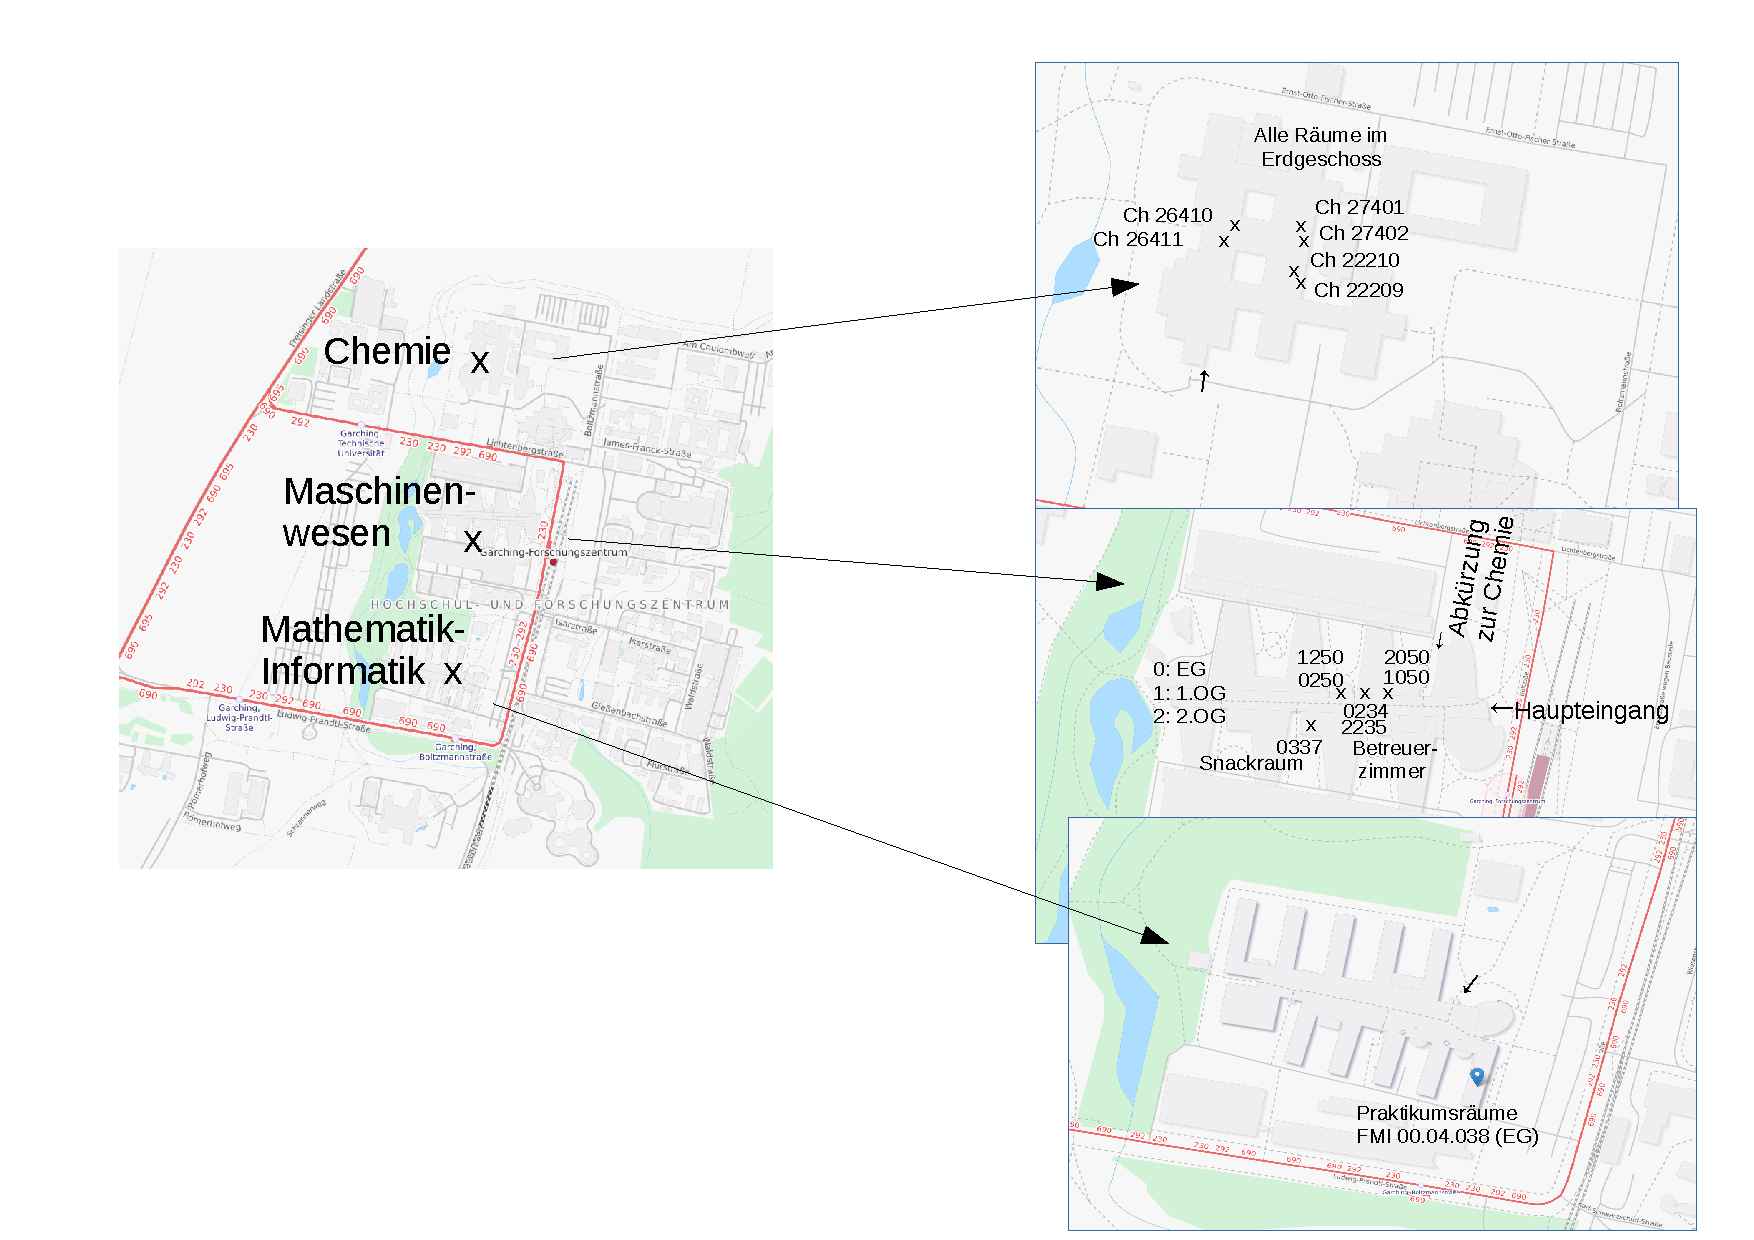
\includegraphics[scale=0.5]{campus_map.pdf}
\end{figure}
\newpage{}\begin{center}{\huge{}\textbf{Stundenplan von Kevin Haag}}\end{center}\textbf{{\large{}Donnerstag}}\nopagebreak \\\begin{tabular} {|p{3cm} p{6cm} p{6cm}| }\hline \textbf{11:30 bis 13:45}&\textbf{Anreise zur TU München}&\textbf{Fakultät Maschinenwesen}\\\hline \textbf{12:00 bis 13:30}&\textbf{Mittagessen}&\textbf{Mensa Garching}\\\hline \textbf{14:00}&\textbf{Begrüßung}&\textbf{CH 26411}\\&Begrüßung, Besprechung des Zeitplans, Ausgabe der individuellen Stundenpläne,...&\\\hline \textbf{14:50 bis 16:20}&\textbf{Experimentieren und Auswerten}&\textbf{CH 26411}\\&Betreuer: Ann-Kathrin Raab&ca. 18 Teilnehmer\\\hline \textbf{16:40 bis 18:10}&\textbf{Klassische Mechanik}&\textbf{MW 1250}\\&Betreuer: Maximilian Marienhagen&ca. 10 Teilnehmer\\\hline \textbf{18:30}&\textbf{Fahrt zur Jugendherberge}&\textbf{}\\\hline \textbf{19:00}&\textbf{Abendessen}&\textbf{Jugendherberge}\\\hline \end{tabular}\\\vspace{5.00000mm}~\\\textbf{{\large{}Freitag}}\nopagebreak \\\begin{tabular} {|p{3cm} p{6cm} p{6cm}| }\hline \textbf{06:30 bis 09:00}&\textbf{Frühstück}&\textbf{Jugendherberge}\\\hline \textbf{09:00 bis 13:00}&\textbf{Besichtigung der Forschungsneutronenquelle FRM II}&\textbf{MW 2050}\\&Betreuer: Felix Wechsler&ca. 28 Teilnehmer\\\hline \textbf{13:00 bis 14:00}&\textbf{Mittagessen}&\textbf{Mensa Garching}\\\hline \textbf{14:20 bis 15:50}&\textbf{Experiment Brückenschaltung}&\textbf{Praktikum Brückenschaltung}\\&Betreuer: Martin Großhauser&ca. 6 Teilnehmer\\\hline \textbf{16:10 bis 17:40}&\textbf{Harmonische Schwingungen}&\textbf{MW 2050}\\&Betreuer: Ilja Göthel&ca. 3 Teilnehmer\\\hline \textbf{18:00 bis 18:20}&\textbf{Erlebnisbericht IPhO}&\textbf{CH 26411}\\\hline \textbf{18:30}&\textbf{Fahrt zur Jugendherberge}&\textbf{}\\\hline \textbf{19:00}&\textbf{Abendessen}&\textbf{Jugendherberge}\\\hline \end{tabular}\\\vspace{5.00000mm}~\\\textbf{{\large{}Samstag}}\nopagebreak \\\begin{tabular} {|p{3cm} p{6cm} p{6cm}| }\hline \textbf{06:30 bis 08:00}&\textbf{Frühstück}&\textbf{Jugendherberge}\\\hline \textbf{08:00}&\textbf{Fahrt zur TU}&\textbf{}\\\hline \textbf{09:00 bis 10:30}&\textbf{Elektrodynamik 1}&\textbf{MW 1250}\\&Betreuer: Maximilian Keitel&ca. 21 Teilnehmer\\\hline \textbf{10:50 bis 12:20}&\textbf{Experiment Pohlsches Rad}&\textbf{Praktikum Pohlsches Rad}\\&Betreuer: Eugen Dizer&ca. 4 Teilnehmer\\\hline \textbf{12:40 bis 14:00}&\textbf{Mittagessen}&\textbf{Fakultät Maschinenwesen}\\\hline \textbf{14:20 bis 15:50}&\textbf{Quanten- und Atomphysik I}&\textbf{CH 22209}\\&Betreuer: Vitaly Andreev&ca. 22 Teilnehmer\\\hline \textbf{16:10 bis 17:40}&\textbf{Komplexe Wechselstromrechnung}&\textbf{MW 0250}\\&Betreuer: Vincent Grande&ca. 13 Teilnehmer\\\hline \textbf{18:00 bis 18:20}&\textbf{Vorstellung GYPT}&\textbf{CH 26411}\\\hline \textbf{18:30}&\textbf{Fahrt zur Jugendherberge}&\textbf{}\\\hline \textbf{19:00}&\textbf{Abendessen}&\textbf{Jugendherberge}\\\hline \end{tabular}\\\vspace{5.00000mm}~\\\textbf{{\large{}Sonntag}}\nopagebreak \\\begin{tabular} {|p{3cm} p{6cm} p{6cm}| }\hline \textbf{06:30 bis 08:00}&\textbf{Frühstück}&\textbf{Jugendherberge}\\\hline \textbf{08:00}&\textbf{Fahrt zur TU}&\textbf{}\\\hline \textbf{09:00 bis 10:30}&\textbf{Wellenoptik}&\textbf{MW 2050}\\&Betreuer: Christopher Pfeiffer&ca. 14 Teilnehmer\\\hline \textbf{10:50 bis 12:20}&\textbf{Aufgabenseminar Quanten- und Atomphysik und Struktur der Materie}&\textbf{MW 1250}\\&Betreuer: Vitaly Andreev&ca. 24 Teilnehmer\\\hline \textbf{12:40 bis 13:00}&\textbf{Verabschiedung}&\textbf{CH 26411}\\\hline \textbf{13:00}&\textbf{Individuelle Abreise}&\textbf{}\\\hline \textbf{13:00 bis 14:00}&\textbf{Mittagessen}&\textbf{}\\\hline \end{tabular}\\\vspace{5.00000mm}~\\
Notfallnummern: \\
Sven Jandura: xxxx xxxxxxxxx \\
Johannes Rothe: xxxx xxxxxxxxx \\

\large Hast du Lust, die Andern vom Seminar wiederzusehen?\\
\normalsize Dann komm doch einfach zum \textbf{Vereinstreffen}. Dazu musst du kein Vereinsmitglied sein. Neben interesannten Vorträgen und Exkursionen sind jede Menge Spiel und Spaß geplant. Schau in einem Monat einfach noch mal auf der Website vorbei. Wir freuen uns, wenn du dabei bist.

\begin{figure}[!h]
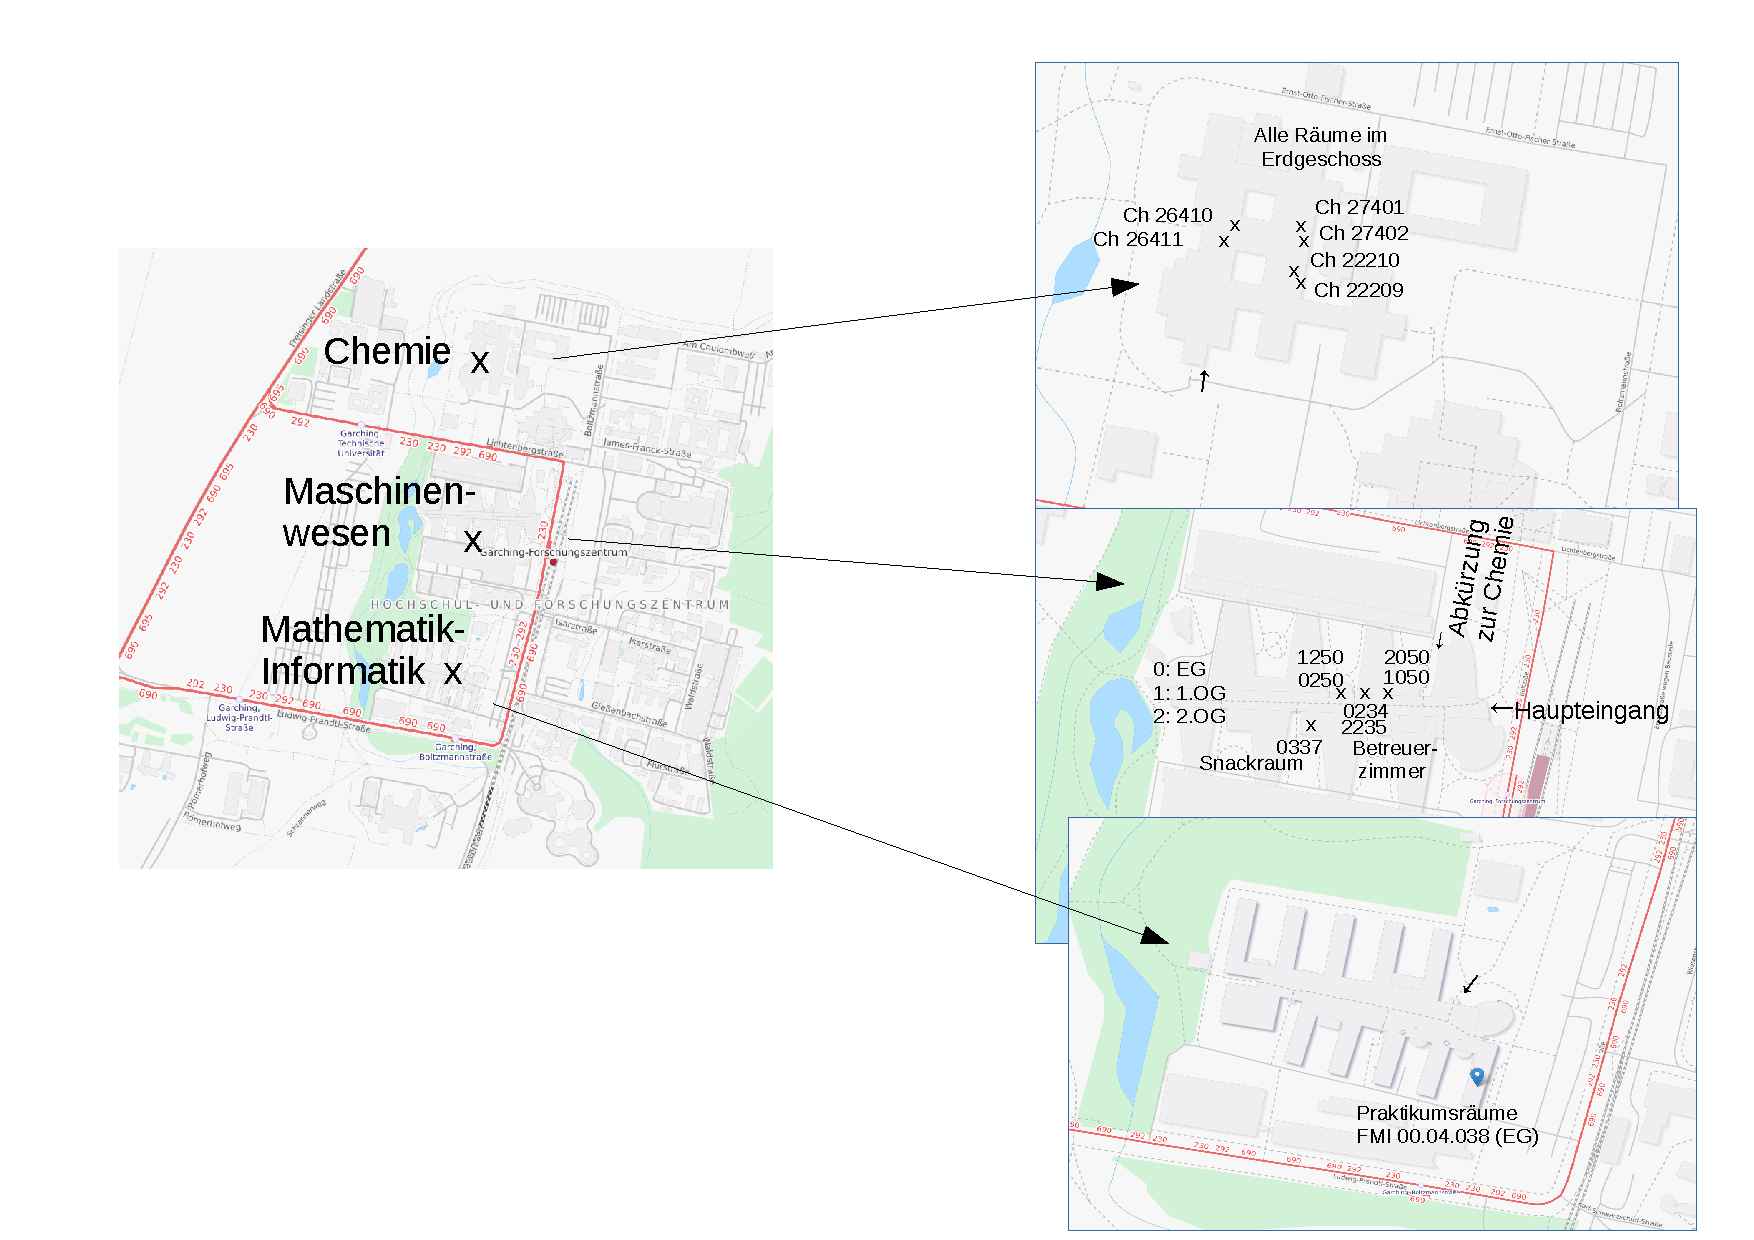
\includegraphics[scale=0.5]{campus_map.pdf}
\end{figure}
\newpage{}\begin{center}{\huge{}\textbf{Stundenplan von Lars Meyer}}\end{center}\textbf{{\large{}Donnerstag}}\nopagebreak \\\begin{tabular} {|p{3cm} p{6cm} p{6cm}| }\hline \textbf{11:30 bis 13:45}&\textbf{Anreise zur TU München}&\textbf{Fakultät Maschinenwesen}\\\hline \textbf{12:00 bis 13:30}&\textbf{Mittagessen}&\textbf{Mensa Garching}\\\hline \textbf{14:00}&\textbf{Begrüßung}&\textbf{CH 26411}\\&Begrüßung, Besprechung des Zeitplans, Ausgabe der individuellen Stundenpläne,...&\\\hline \textbf{14:50 bis 16:20}&\textbf{Einführung ins Differenzieren}&\textbf{MW 1050}\\&Betreuer: Ilja Göthel&ca. 6 Teilnehmer\\\hline \textbf{16:40 bis 18:10}&\textbf{Näherungsmethoden}&\textbf{MW 0234}\\&Betreuer: Ilja Göthel&ca. 13 Teilnehmer\\\hline \textbf{18:30}&\textbf{Fahrt zur Jugendherberge}&\textbf{}\\\hline \textbf{19:00}&\textbf{Abendessen}&\textbf{Jugendherberge}\\\hline \end{tabular}\\\vspace{5.00000mm}~\\\textbf{{\large{}Freitag}}\nopagebreak \\\begin{tabular} {|p{3cm} p{6cm} p{6cm}| }\hline \textbf{06:30 bis 09:00}&\textbf{Frühstück}&\textbf{Jugendherberge}\\\hline \textbf{09:00 bis 13:00}&frei&\\\hline \textbf{13:00 bis 14:00}&\textbf{Mittagessen}&\textbf{Mensa Garching}\\\hline \textbf{14:20 bis 15:50}&\textbf{Kernphysik}&\textbf{MW 0250}\\&Betreuer: Johannes Rothe&ca. 18 Teilnehmer\\\hline \textbf{16:10 bis 17:40}&\textbf{Experiment spezifische Elektronenladung}&\textbf{Praktikum spezifische Elektronenladung}\\&Betreuer: Felix Wechsler&ca. 6 Teilnehmer\\\hline \textbf{18:00 bis 18:20}&\textbf{Erlebnisbericht IPhO}&\textbf{CH 26411}\\\hline \textbf{18:30}&\textbf{Fahrt zur Jugendherberge}&\textbf{}\\\hline \textbf{19:00}&\textbf{Abendessen}&\textbf{Jugendherberge}\\\hline \end{tabular}\\\vspace{5.00000mm}~\\\textbf{{\large{}Samstag}}\nopagebreak \\\begin{tabular} {|p{3cm} p{6cm} p{6cm}| }\hline \textbf{06:30 bis 08:00}&\textbf{Frühstück}&\textbf{Jugendherberge}\\\hline \textbf{08:00}&\textbf{Fahrt zur TU}&\textbf{}\\\hline \textbf{09:00 bis 10:30}&\textbf{Harmonische Schwingungen}&\textbf{MW 0250}\\&Betreuer: Ilja Göthel&ca. 9 Teilnehmer\\\hline \textbf{10:50 bis 12:20}&\textbf{Experiment Brennstoffzelle}&\textbf{Praktikum Brennstoffzelle}\\&Betreuer: Aaron Wild&ca. 6 Teilnehmer\\\hline \textbf{12:40 bis 14:00}&\textbf{Mittagessen}&\textbf{Fakultät Maschinenwesen}\\\hline \textbf{14:20 bis 15:50}&\textbf{Quanten- und Atomphysik I}&\textbf{CH 22209}\\&Betreuer: Vitaly Andreev&ca. 22 Teilnehmer\\\hline \textbf{16:10 bis 17:40}&\textbf{Aufgabenseminar klassische Mechanik}&\textbf{MW 2050}\\&Betreuer: Aaron Wild&ca. 5 Teilnehmer\\\hline \textbf{18:00 bis 18:20}&\textbf{Vorstellung GYPT}&\textbf{CH 26411}\\\hline \textbf{18:30}&\textbf{Fahrt zur Jugendherberge}&\textbf{}\\\hline \textbf{19:00}&\textbf{Abendessen}&\textbf{Jugendherberge}\\\hline \end{tabular}\\\vspace{5.00000mm}~\\\textbf{{\large{}Sonntag}}\nopagebreak \\\begin{tabular} {|p{3cm} p{6cm} p{6cm}| }\hline \textbf{06:30 bis 08:00}&\textbf{Frühstück}&\textbf{Jugendherberge}\\\hline \textbf{08:00}&\textbf{Fahrt zur TU}&\textbf{}\\\hline \textbf{09:00 bis 10:30}&\textbf{Spezielle Relativitätstheorie}&\textbf{MW 0250}\\&Betreuer: Johannes Rothe&ca. 12 Teilnehmer\\\hline \textbf{10:50 bis 12:20}&\textbf{Relativistische Teilchenphysik}&\textbf{CH 22210}\\&Betreuer: Lars Dehlwes&ca. 11 Teilnehmer\\\hline \textbf{12:40 bis 13:00}&\textbf{Verabschiedung}&\textbf{CH 26411}\\\hline \textbf{13:00}&\textbf{Individuelle Abreise}&\textbf{}\\\hline \textbf{13:00 bis 14:00}&\textbf{Mittagessen}&\textbf{}\\\hline \end{tabular}\\\vspace{5.00000mm}~\\
Notfallnummern: \\
Sven Jandura: xxxx xxxxxxxxx \\
Johannes Rothe: xxxx xxxxxxxxx \\

\large Hast du Lust, die Andern vom Seminar wiederzusehen?\\
\normalsize Dann komm doch einfach zum \textbf{Vereinstreffen}. Dazu musst du kein Vereinsmitglied sein. Neben interesannten Vorträgen und Exkursionen sind jede Menge Spiel und Spaß geplant. Schau in einem Monat einfach noch mal auf der Website vorbei. Wir freuen uns, wenn du dabei bist.

\begin{figure}[!h]
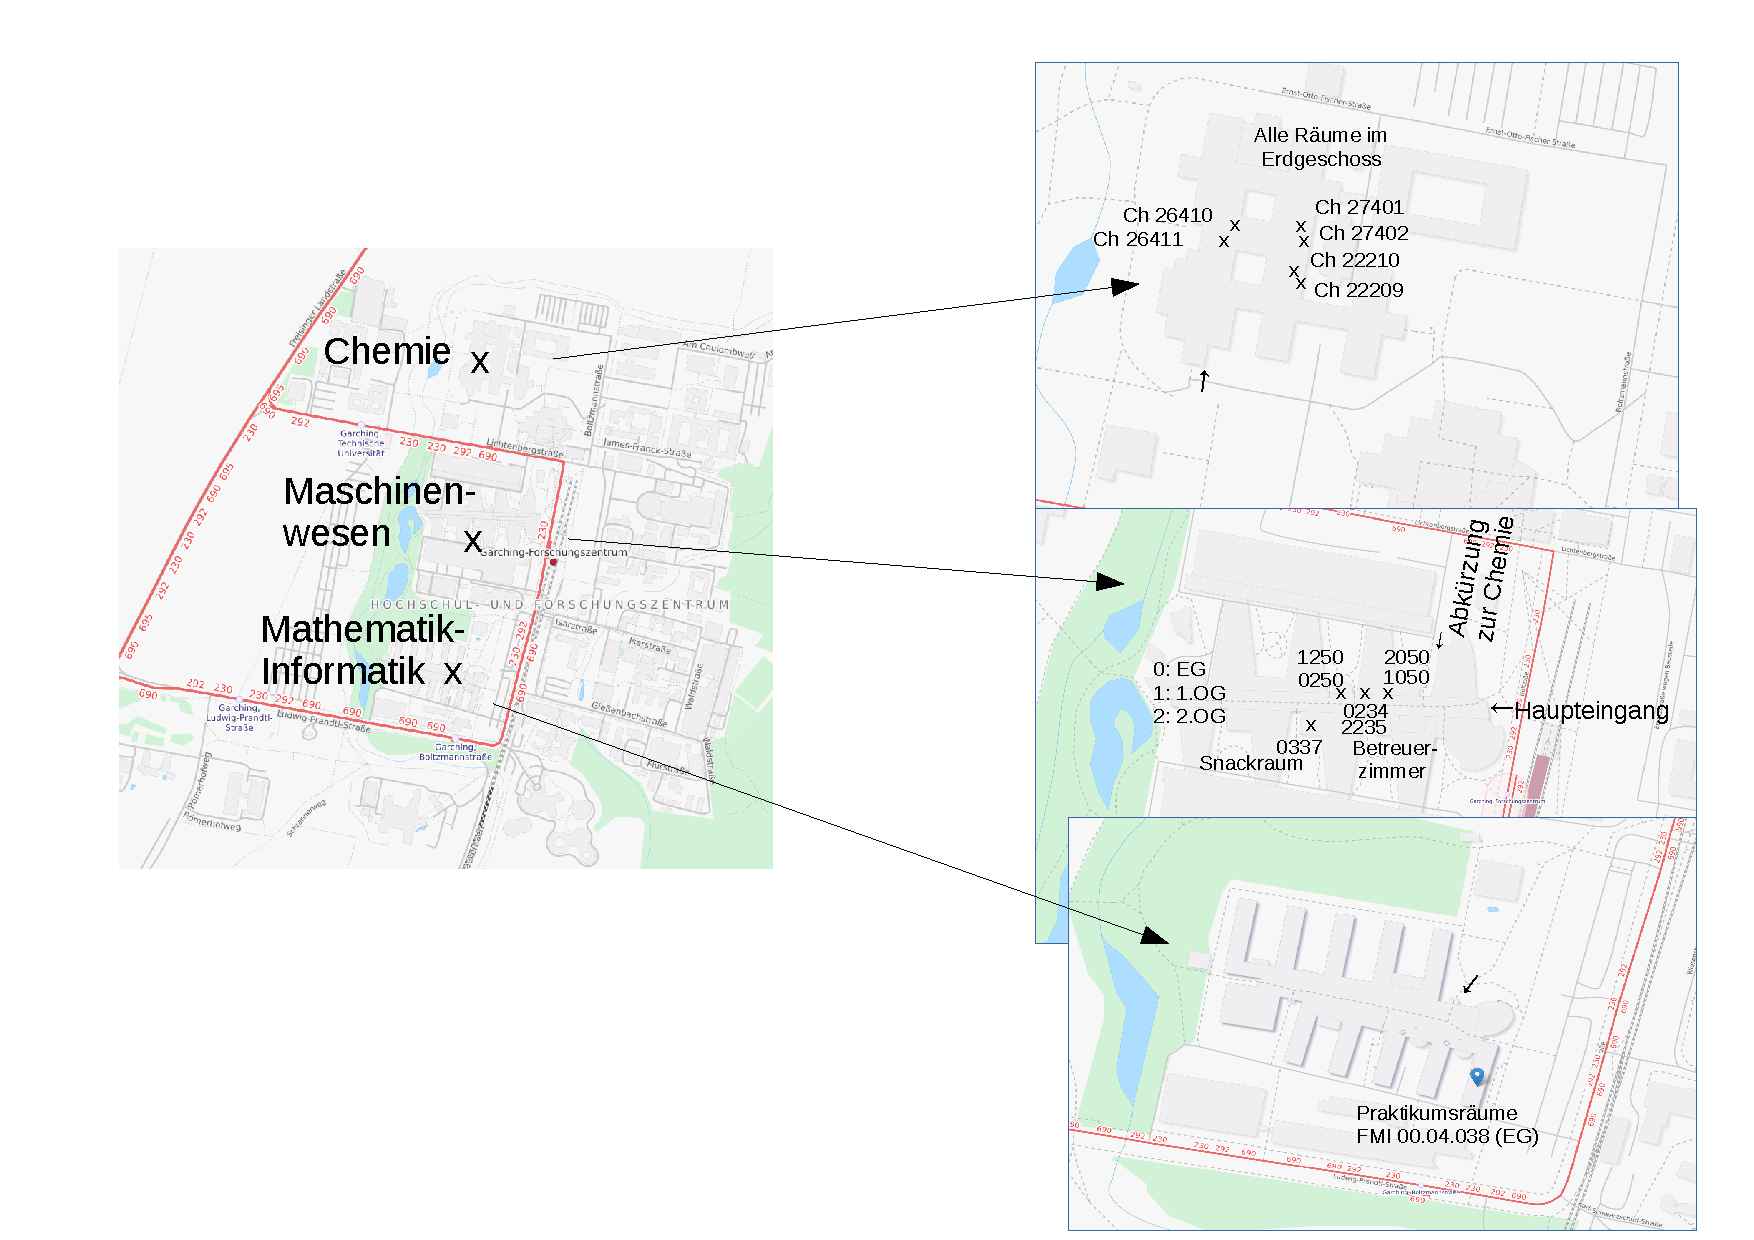
\includegraphics[scale=0.5]{campus_map.pdf}
\end{figure}
\newpage{}\begin{center}{\huge{}\textbf{Stundenplan von Lennart Müller}}\end{center}\textbf{{\large{}Donnerstag}}\nopagebreak \\\begin{tabular} {|p{3cm} p{6cm} p{6cm}| }\hline \textbf{11:30 bis 13:45}&\textbf{Anreise zur TU München}&\textbf{Fakultät Maschinenwesen}\\\hline \textbf{12:00 bis 13:30}&\textbf{Mittagessen}&\textbf{Mensa Garching}\\\hline \textbf{14:00}&\textbf{Begrüßung}&\textbf{CH 26411}\\&Begrüßung, Besprechung des Zeitplans, Ausgabe der individuellen Stundenpläne,...&\\\hline \textbf{14:50 bis 16:20}&\textbf{Elektrische Schaltungen}&\textbf{MW 0250}\\&Betreuer: Christopher Pfeiffer&ca. 16 Teilnehmer\\\hline \textbf{16:40 bis 18:10}&\textbf{Geometrische Optik}&\textbf{MW 0250}\\&Betreuer: Christopher Pfeiffer&ca. 13 Teilnehmer\\\hline \textbf{18:30}&\textbf{Fahrt zur Jugendherberge}&\textbf{}\\\hline \textbf{19:00}&\textbf{Abendessen}&\textbf{Jugendherberge}\\\hline \end{tabular}\\\vspace{5.00000mm}~\\\textbf{{\large{}Freitag}}\nopagebreak \\\begin{tabular} {|p{3cm} p{6cm} p{6cm}| }\hline \textbf{06:30 bis 09:00}&\textbf{Frühstück}&\textbf{Jugendherberge}\\\hline \textbf{09:00 bis 13:00}&frei&\\\hline \textbf{13:00 bis 14:00}&\textbf{Mittagessen}&\textbf{Mensa Garching}\\\hline \textbf{14:20 bis 15:50}&\textbf{Kernphysik}&\textbf{MW 0250}\\&Betreuer: Johannes Rothe&ca. 18 Teilnehmer\\\hline \textbf{16:10 bis 17:40}&\textbf{Experiment Oszilloskop}&\textbf{Praktikum Oszilloskop}\\&Betreuer: Christopher Pfeiffer&ca. 6 Teilnehmer\\\hline \textbf{18:00 bis 18:20}&\textbf{Erlebnisbericht IPhO}&\textbf{CH 26411}\\\hline \textbf{18:30}&\textbf{Fahrt zur Jugendherberge}&\textbf{}\\\hline \textbf{19:00}&\textbf{Abendessen}&\textbf{Jugendherberge}\\\hline \end{tabular}\\\vspace{5.00000mm}~\\\textbf{{\large{}Samstag}}\nopagebreak \\\begin{tabular} {|p{3cm} p{6cm} p{6cm}| }\hline \textbf{06:30 bis 08:00}&\textbf{Frühstück}&\textbf{Jugendherberge}\\\hline \textbf{08:00}&\textbf{Fahrt zur TU}&\textbf{}\\\hline \textbf{09:00 bis 10:30}&\textbf{Harmonische Schwingungen}&\textbf{MW 0250}\\&Betreuer: Ilja Göthel&ca. 9 Teilnehmer\\\hline \textbf{10:50 bis 12:20}&\textbf{Klassische Mechanik}&\textbf{MW 1050}\\&Betreuer: Maximilian Marienhagen&ca. 3 Teilnehmer\\\hline \textbf{12:40 bis 14:00}&\textbf{Mittagessen}&\textbf{Fakultät Maschinenwesen}\\\hline \textbf{14:20 bis 15:50}&\textbf{Bestimmung des Brechungskoeffizienten von Plexiglas}&\textbf{MW 0234}\\&Betreuer: Lilith Diringer&ca. 8 Teilnehmer\\\hline \textbf{16:10 bis 17:40}&\textbf{Bestimmung des Brechungskoeffizienten von Wasser}&\textbf{MW 0234}\\&Betreuer: Lilith Diringer&ca. 8 Teilnehmer\\\hline \textbf{18:00 bis 18:20}&\textbf{Vorstellung GYPT}&\textbf{CH 26411}\\\hline \textbf{18:30}&\textbf{Fahrt zur Jugendherberge}&\textbf{}\\\hline \textbf{19:00}&\textbf{Abendessen}&\textbf{Jugendherberge}\\\hline \end{tabular}\\\vspace{5.00000mm}~\\\textbf{{\large{}Sonntag}}\nopagebreak \\\begin{tabular} {|p{3cm} p{6cm} p{6cm}| }\hline \textbf{06:30 bis 08:00}&\textbf{Frühstück}&\textbf{Jugendherberge}\\\hline \textbf{08:00}&\textbf{Fahrt zur TU}&\textbf{}\\\hline \textbf{09:00 bis 10:30}&\textbf{Aufgabenseminar Wärmelehre}&\textbf{CH 22209}\\&Betreuer: Maximilian Marienhagen&ca. 9 Teilnehmer\\\hline \textbf{10:50 bis 12:20}&\textbf{Rotationsbewegungen}&\textbf{CH 26410}\\&Betreuer: Vincent Grande&ca. 9 Teilnehmer\\\hline \textbf{12:40 bis 13:00}&\textbf{Verabschiedung}&\textbf{CH 26411}\\\hline \textbf{13:00}&\textbf{Individuelle Abreise}&\textbf{}\\\hline \textbf{13:00 bis 14:00}&\textbf{Mittagessen}&\textbf{}\\\hline \end{tabular}\\\vspace{5.00000mm}~\\
Notfallnummern: \\
Sven Jandura: xxxx xxxxxxxxx \\
Johannes Rothe: xxxx xxxxxxxxx \\

\large Hast du Lust, die Andern vom Seminar wiederzusehen?\\
\normalsize Dann komm doch einfach zum \textbf{Vereinstreffen}. Dazu musst du kein Vereinsmitglied sein. Neben interesannten Vorträgen und Exkursionen sind jede Menge Spiel und Spaß geplant. Schau in einem Monat einfach noch mal auf der Website vorbei. Wir freuen uns, wenn du dabei bist.

\begin{figure}[!h]
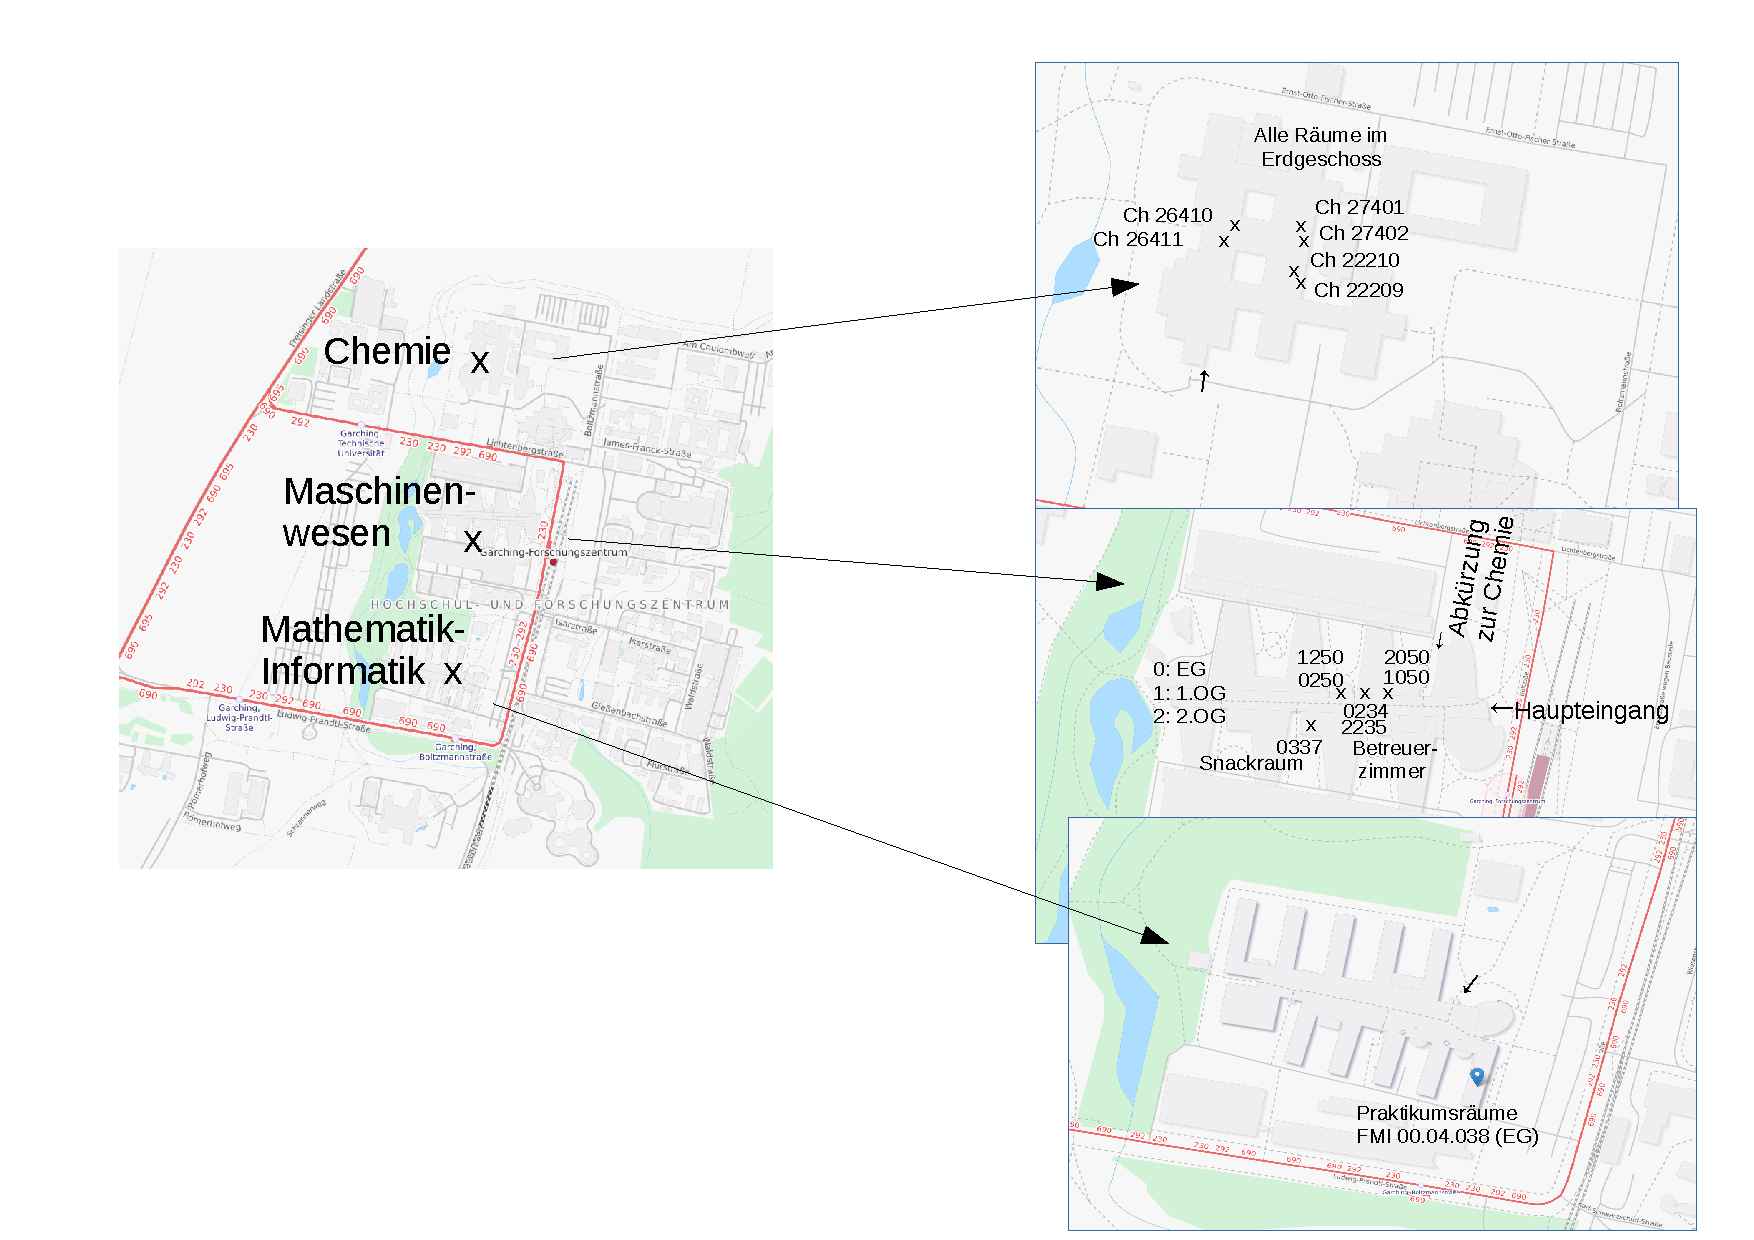
\includegraphics[scale=0.5]{campus_map.pdf}
\end{figure}
\newpage{}\begin{center}{\huge{}\textbf{Stundenplan von Lennart Brandt}}\end{center}\textbf{{\large{}Donnerstag}}\nopagebreak \\\begin{tabular} {|p{3cm} p{6cm} p{6cm}| }\hline \textbf{11:30 bis 13:45}&\textbf{Anreise zur TU München}&\textbf{Fakultät Maschinenwesen}\\\hline \textbf{12:00 bis 13:30}&\textbf{Mittagessen}&\textbf{Mensa Garching}\\\hline \textbf{14:00}&\textbf{Begrüßung}&\textbf{CH 26411}\\&Begrüßung, Besprechung des Zeitplans, Ausgabe der individuellen Stundenpläne,...&\\\hline \textbf{14:50 bis 16:20}&\textbf{Quanten- und Atomphysik I}&\textbf{CH 26410}\\&Betreuer: Ismail Achmed-Zade&ca. 28 Teilnehmer\\\hline \textbf{16:40 bis 18:10}&\textbf{Klassische Mechanik}&\textbf{MW 1250}\\&Betreuer: Maximilian Marienhagen&ca. 10 Teilnehmer\\\hline \textbf{18:30}&\textbf{Fahrt zur Jugendherberge}&\textbf{}\\\hline \textbf{19:00}&\textbf{Abendessen}&\textbf{Jugendherberge}\\\hline \end{tabular}\\\vspace{5.00000mm}~\\\textbf{{\large{}Freitag}}\nopagebreak \\\begin{tabular} {|p{3cm} p{6cm} p{6cm}| }\hline \textbf{06:30 bis 09:00}&\textbf{Frühstück}&\textbf{Jugendherberge}\\\hline \textbf{09:00 bis 13:00}&frei&\\\hline \textbf{13:00 bis 14:00}&\textbf{Mittagessen}&\textbf{Mensa Garching}\\\hline \textbf{14:20 bis 15:50}&\textbf{Kernphysik}&\textbf{MW 0250}\\&Betreuer: Johannes Rothe&ca. 18 Teilnehmer\\\hline \textbf{16:10 bis 17:40}&\textbf{Näherungsmethoden}&\textbf{CH 26410}\\&Betreuer: Vincent Grande&ca. 11 Teilnehmer\\\hline \textbf{18:00 bis 18:20}&\textbf{Erlebnisbericht IPhO}&\textbf{CH 26411}\\\hline \textbf{18:30}&\textbf{Fahrt zur Jugendherberge}&\textbf{}\\\hline \textbf{19:00}&\textbf{Abendessen}&\textbf{Jugendherberge}\\\hline \end{tabular}\\\vspace{5.00000mm}~\\\textbf{{\large{}Samstag}}\nopagebreak \\\begin{tabular} {|p{3cm} p{6cm} p{6cm}| }\hline \textbf{06:30 bis 08:00}&\textbf{Frühstück}&\textbf{Jugendherberge}\\\hline \textbf{08:00}&\textbf{Fahrt zur TU}&\textbf{}\\\hline \textbf{09:00 bis 10:30}&\textbf{Experimentieren und Auswerten}&\textbf{CH 26411}\\&Betreuer: Ann-Kathrin Raab&ca. 18 Teilnehmer\\\hline \textbf{10:50 bis 12:20}&\textbf{Geometrische Optik}&\textbf{MW 0234}\\&Betreuer: Christopher Pfeiffer&ca. 3 Teilnehmer\\\hline \textbf{12:40 bis 14:00}&\textbf{Mittagessen}&\textbf{Fakultät Maschinenwesen}\\\hline \textbf{14:20 bis 15:50}&\textbf{Thermodynamik 1}&\textbf{MW 1250}\\&Betreuer: Maximilian Marienhagen&ca. 9 Teilnehmer\\\hline \textbf{16:10 bis 17:40}&\textbf{Bestimmung des Brechungskoeffizienten von Wasser}&\textbf{MW 0234}\\&Betreuer: Lilith Diringer&ca. 8 Teilnehmer\\\hline \textbf{18:00 bis 18:20}&\textbf{Vorstellung GYPT}&\textbf{CH 26411}\\\hline \textbf{18:30}&\textbf{Fahrt zur Jugendherberge}&\textbf{}\\\hline \textbf{19:00}&\textbf{Abendessen}&\textbf{Jugendherberge}\\\hline \end{tabular}\\\vspace{5.00000mm}~\\\textbf{{\large{}Sonntag}}\nopagebreak \\\begin{tabular} {|p{3cm} p{6cm} p{6cm}| }\hline \textbf{06:30 bis 08:00}&\textbf{Frühstück}&\textbf{Jugendherberge}\\\hline \textbf{08:00}&\textbf{Fahrt zur TU}&\textbf{}\\\hline \textbf{09:00 bis 10:30}&\textbf{Spezielle Relativitätstheorie}&\textbf{MW 0250}\\&Betreuer: Johannes Rothe&ca. 12 Teilnehmer\\\hline \textbf{10:50 bis 12:20}&\textbf{Aufgabenseminar klassische Mechanik}&\textbf{CH 22209}\\&Betreuer: Aaron Wild&ca. 11 Teilnehmer\\\hline \textbf{12:40 bis 13:00}&\textbf{Verabschiedung}&\textbf{CH 26411}\\\hline \textbf{13:00}&\textbf{Individuelle Abreise}&\textbf{}\\\hline \textbf{13:00 bis 14:00}&\textbf{Mittagessen}&\textbf{}\\\hline \end{tabular}\\\vspace{5.00000mm}~\\
Notfallnummern: \\
Sven Jandura: xxxx xxxxxxxxx \\
Johannes Rothe: xxxx xxxxxxxxx \\

\large Hast du Lust, die Andern vom Seminar wiederzusehen?\\
\normalsize Dann komm doch einfach zum \textbf{Vereinstreffen}. Dazu musst du kein Vereinsmitglied sein. Neben interesannten Vorträgen und Exkursionen sind jede Menge Spiel und Spaß geplant. Schau in einem Monat einfach noch mal auf der Website vorbei. Wir freuen uns, wenn du dabei bist.

\begin{figure}[!h]
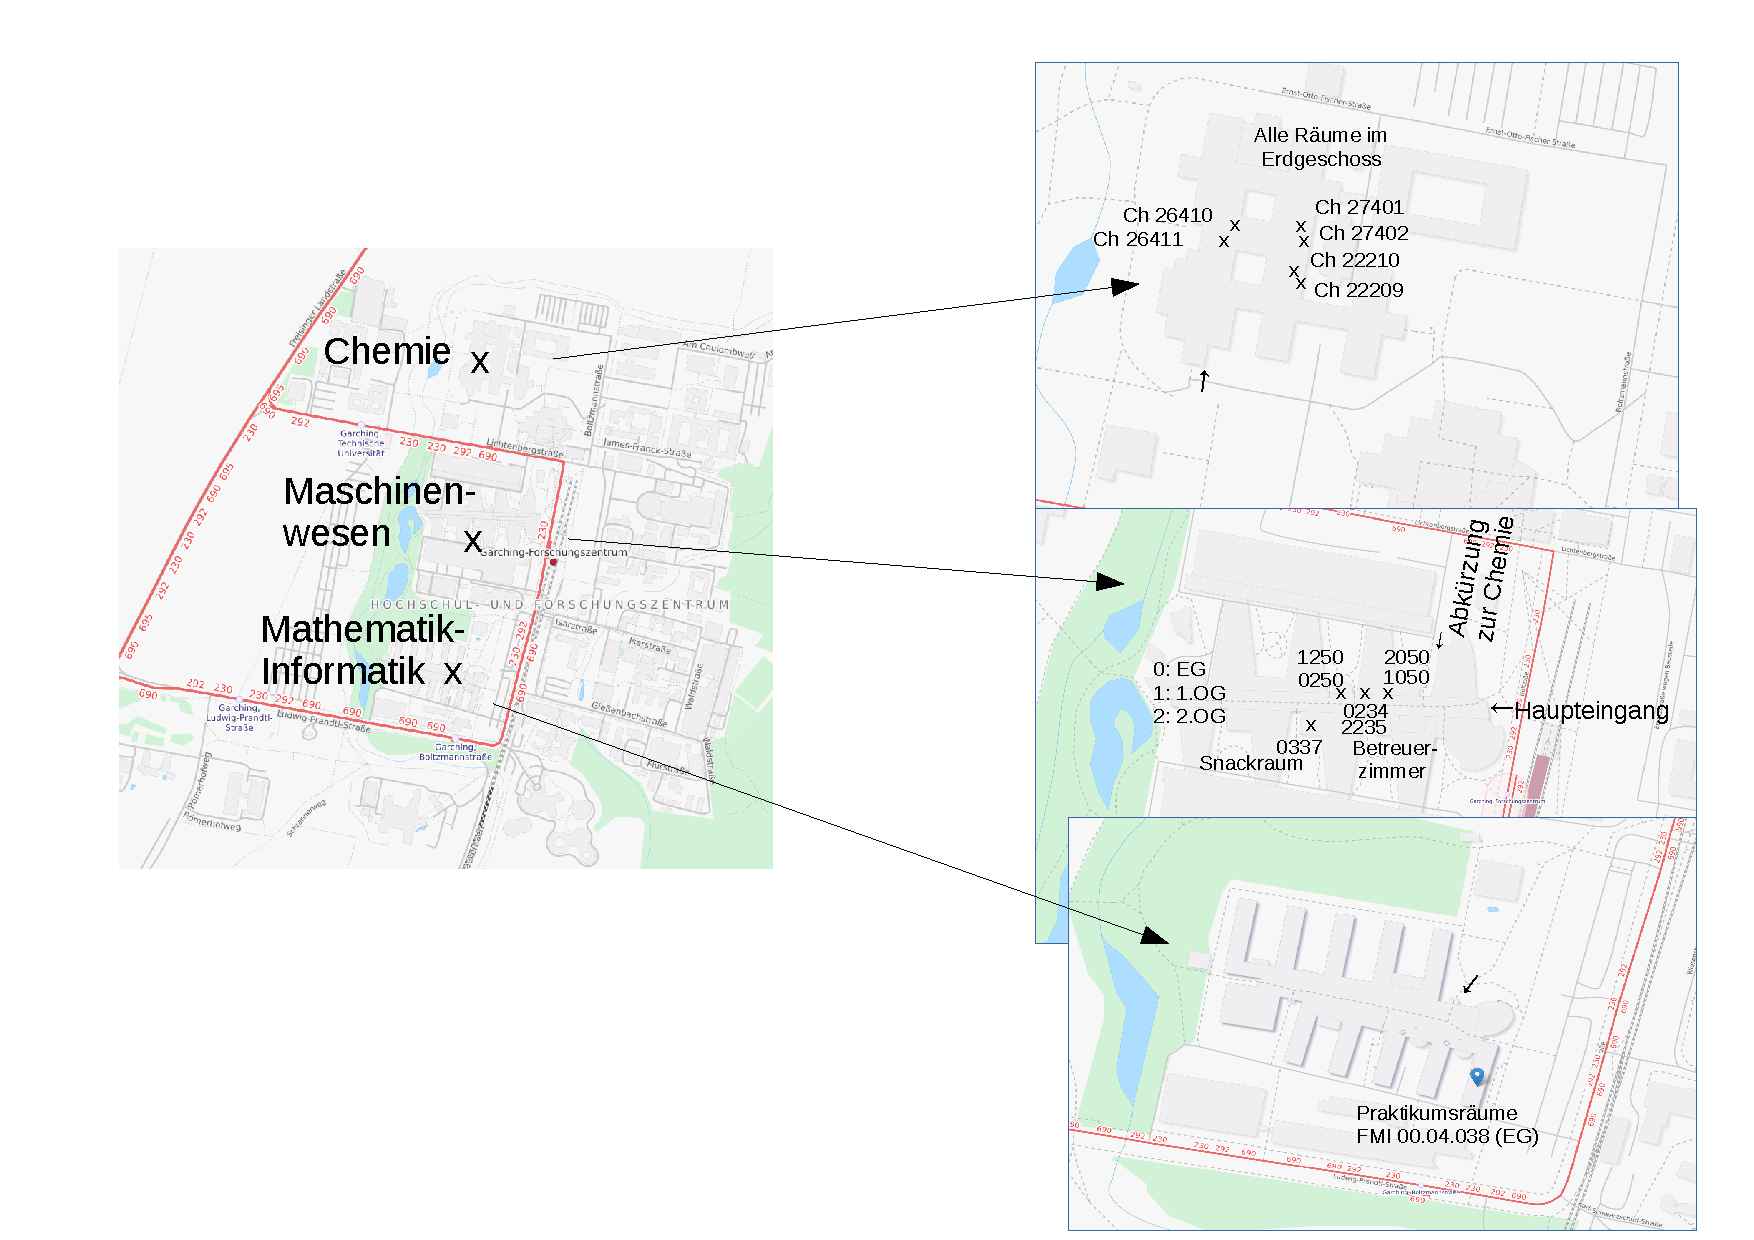
\includegraphics[scale=0.5]{campus_map.pdf}
\end{figure}
\newpage{}\begin{center}{\huge{}\textbf{Stundenplan von Lina Renke}}\end{center}\textbf{{\large{}Donnerstag}}\nopagebreak \\\begin{tabular} {|p{3cm} p{6cm} p{6cm}| }\hline \textbf{11:30 bis 13:45}&\textbf{Anreise zur TU München}&\textbf{Fakultät Maschinenwesen}\\\hline \textbf{12:00 bis 13:30}&\textbf{Mittagessen}&\textbf{Mensa Garching}\\\hline \textbf{14:00}&\textbf{Begrüßung}&\textbf{CH 26411}\\&Begrüßung, Besprechung des Zeitplans, Ausgabe der individuellen Stundenpläne,...&\\\hline \textbf{14:50 bis 16:20}&\textbf{Thermodynamik 1}&\textbf{MW 1250}\\&Betreuer: Maximilian Marienhagen&ca. 12 Teilnehmer\\\hline \textbf{16:40 bis 18:10}&\textbf{Experimentieren und Auswerten}&\textbf{CH 26411}\\&Betreuer: Ann-Kathrin Raab&ca. 15 Teilnehmer\\\hline \textbf{18:30}&\textbf{Fahrt zur Jugendherberge}&\textbf{}\\\hline \textbf{19:00}&\textbf{Abendessen}&\textbf{Jugendherberge}\\\hline \end{tabular}\\\vspace{5.00000mm}~\\\textbf{{\large{}Freitag}}\nopagebreak \\\begin{tabular} {|p{3cm} p{6cm} p{6cm}| }\hline \textbf{06:30 bis 09:00}&\textbf{Frühstück}&\textbf{Jugendherberge}\\\hline \textbf{09:00 bis 13:00}&frei&\\\hline \textbf{13:00 bis 14:00}&\textbf{Mittagessen}&\textbf{Mensa Garching}\\\hline \textbf{14:20 bis 15:50}&\textbf{Aufgabenseminar Wärmelehre}&\textbf{MW 2050}\\&Betreuer: Maximilian Marienhagen&ca. 9 Teilnehmer\\\hline \textbf{16:10 bis 17:40}&\textbf{Experiment Magnetismus}&\textbf{Praktikum Magnetismus}\\&Betreuer: Lars Dehlwes&ca. 6 Teilnehmer\\\hline \textbf{18:00 bis 18:20}&\textbf{Erlebnisbericht IPhO}&\textbf{CH 26411}\\\hline \textbf{18:30}&\textbf{Fahrt zur Jugendherberge}&\textbf{}\\\hline \textbf{19:00}&\textbf{Abendessen}&\textbf{Jugendherberge}\\\hline \end{tabular}\\\vspace{5.00000mm}~\\\textbf{{\large{}Samstag}}\nopagebreak \\\begin{tabular} {|p{3cm} p{6cm} p{6cm}| }\hline \textbf{06:30 bis 08:00}&\textbf{Frühstück}&\textbf{Jugendherberge}\\\hline \textbf{08:00}&\textbf{Fahrt zur TU}&\textbf{}\\\hline \textbf{09:00 bis 10:30}&\textbf{Experiment Millikan-Versuch}&\textbf{Praktikum Millikan-Versuch}\\&Betreuer: Samuel Moll&ca. 6 Teilnehmer\\\hline \textbf{10:50 bis 12:20}&\textbf{Spezielle Relativitätstheorie}&\textbf{MW 0250}\\&Betreuer: Johannes Rothe&ca. 12 Teilnehmer\\\hline \textbf{12:40 bis 14:00}&\textbf{Mittagessen}&\textbf{Fakultät Maschinenwesen}\\\hline \textbf{14:20 bis 15:50}&\textbf{Bestimmung des Brechungskoeffizienten von Plexiglas}&\textbf{MW 0234}\\&Betreuer: Lilith Diringer&ca. 8 Teilnehmer\\\hline \textbf{16:10 bis 17:40}&\textbf{Aufgabenseminar klassische Mechanik}&\textbf{MW 2050}\\&Betreuer: Aaron Wild&ca. 5 Teilnehmer\\\hline \textbf{18:00 bis 18:20}&\textbf{Vorstellung GYPT}&\textbf{CH 26411}\\\hline \textbf{18:30}&\textbf{Fahrt zur Jugendherberge}&\textbf{}\\\hline \textbf{19:00}&\textbf{Abendessen}&\textbf{Jugendherberge}\\\hline \end{tabular}\\\vspace{5.00000mm}~\\\textbf{{\large{}Sonntag}}\nopagebreak \\\begin{tabular} {|p{3cm} p{6cm} p{6cm}| }\hline \textbf{06:30 bis 08:00}&\textbf{Frühstück}&\textbf{Jugendherberge}\\\hline \textbf{08:00}&\textbf{Fahrt zur TU}&\textbf{}\\\hline \textbf{09:00 bis 10:30}&\textbf{Elektronik}&\textbf{CH 26410}\\&Betreuer: Martin Großhauser&ca. 10 Teilnehmer\\\hline \textbf{10:50 bis 12:20}&\textbf{Rotationsbewegungen}&\textbf{CH 26410}\\&Betreuer: Vincent Grande&ca. 9 Teilnehmer\\\hline \textbf{12:40 bis 13:00}&\textbf{Verabschiedung}&\textbf{CH 26411}\\\hline \textbf{13:00}&\textbf{Individuelle Abreise}&\textbf{}\\\hline \textbf{13:00 bis 14:00}&\textbf{Mittagessen}&\textbf{}\\\hline \end{tabular}\\\vspace{5.00000mm}~\\
Notfallnummern: \\
Sven Jandura: xxxx xxxxxxxxx \\
Johannes Rothe: xxxx xxxxxxxxx \\

\large Hast du Lust, die Andern vom Seminar wiederzusehen?\\
\normalsize Dann komm doch einfach zum \textbf{Vereinstreffen}. Dazu musst du kein Vereinsmitglied sein. Neben interesannten Vorträgen und Exkursionen sind jede Menge Spiel und Spaß geplant. Schau in einem Monat einfach noch mal auf der Website vorbei. Wir freuen uns, wenn du dabei bist.

\begin{figure}[!h]
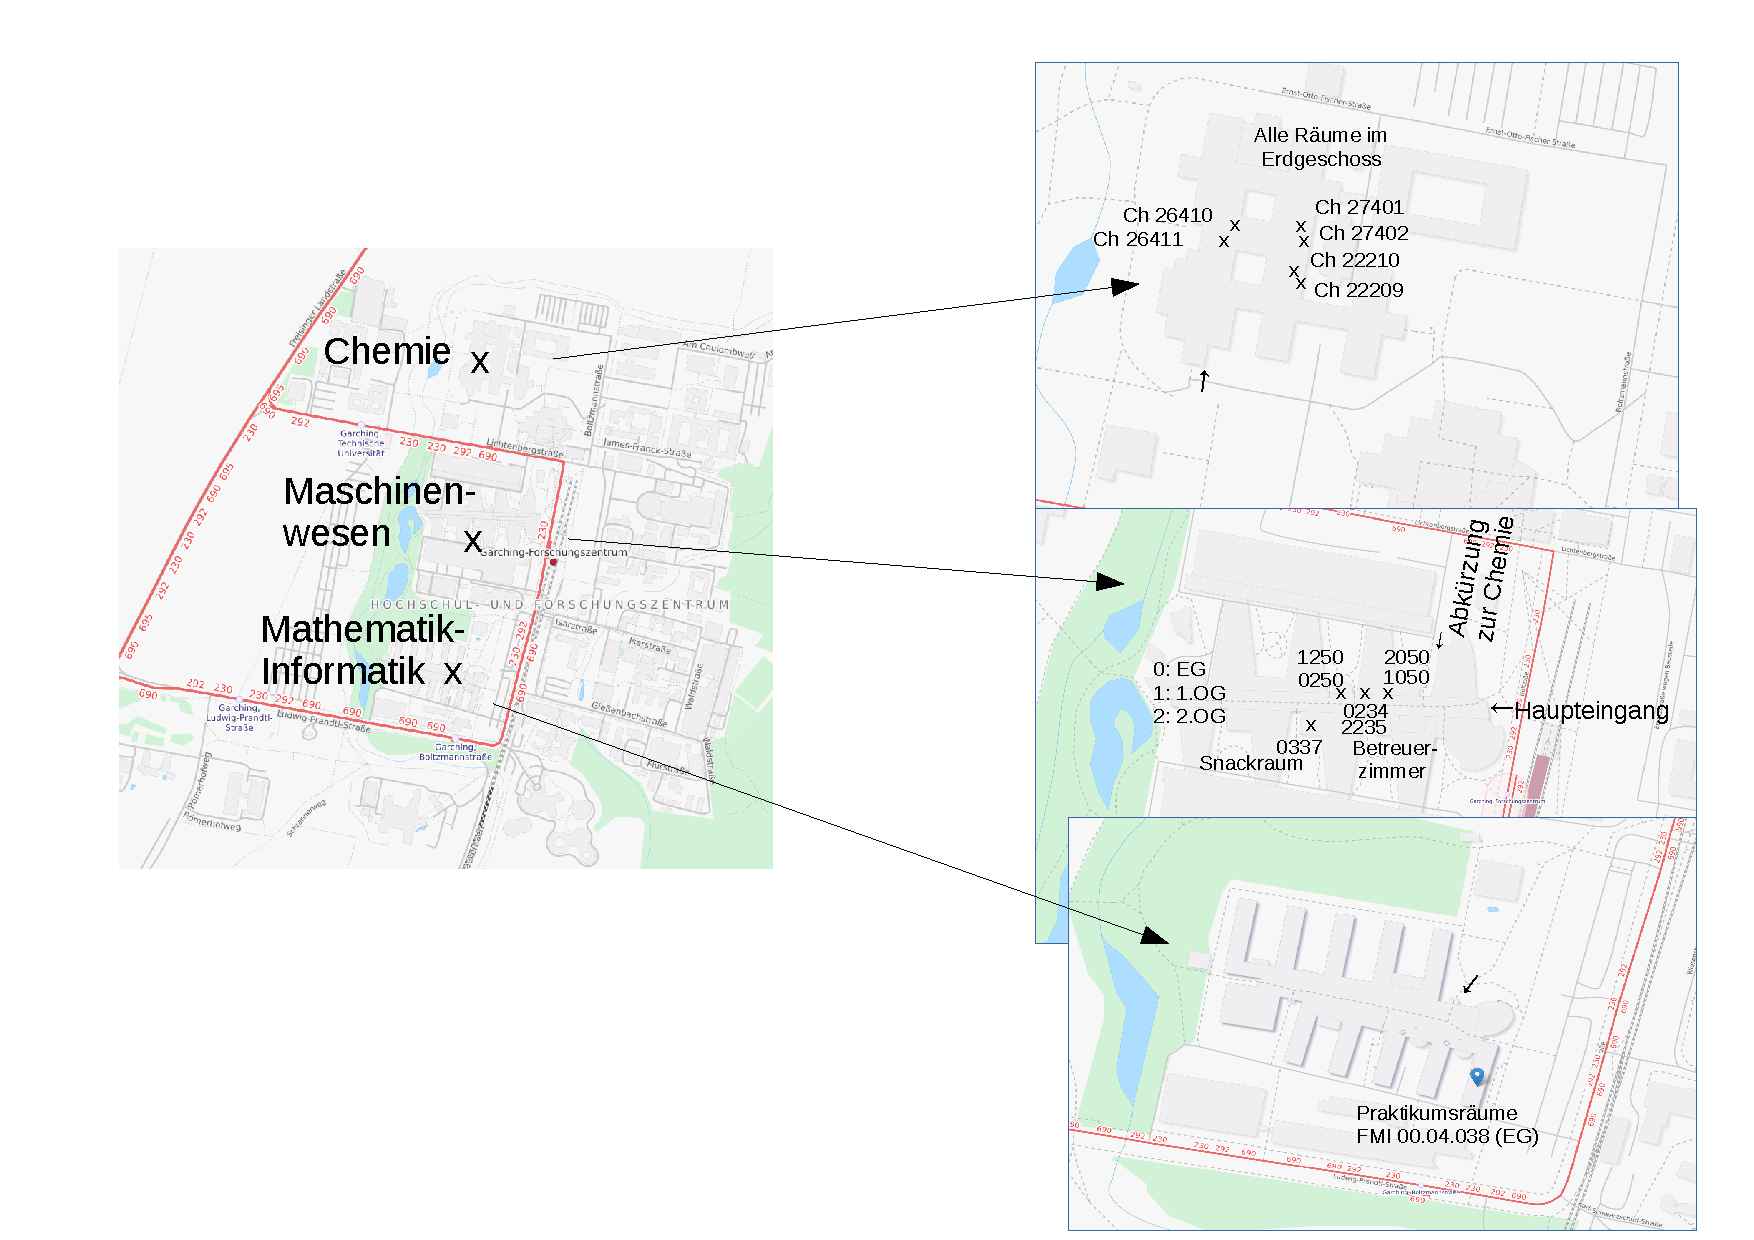
\includegraphics[scale=0.5]{campus_map.pdf}
\end{figure}
\newpage{}\begin{center}{\huge{}\textbf{Stundenplan von Linus Götzfried}}\end{center}\textbf{{\large{}Donnerstag}}\nopagebreak \\\begin{tabular} {|p{3cm} p{6cm} p{6cm}| }\hline \textbf{11:30 bis 13:45}&\textbf{Anreise zur TU München}&\textbf{Fakultät Maschinenwesen}\\\hline \textbf{12:00 bis 13:30}&\textbf{Mittagessen}&\textbf{Mensa Garching}\\\hline \textbf{14:00}&\textbf{Begrüßung}&\textbf{CH 26411}\\&Begrüßung, Besprechung des Zeitplans, Ausgabe der individuellen Stundenpläne,...&\\\hline \textbf{14:50 bis 16:20}&\textbf{Einführung ins Differenzieren}&\textbf{MW 1050}\\&Betreuer: Ilja Göthel&ca. 6 Teilnehmer\\\hline \textbf{16:40 bis 18:10}&\textbf{Experimentieren und Auswerten}&\textbf{CH 26411}\\&Betreuer: Ann-Kathrin Raab&ca. 15 Teilnehmer\\\hline \textbf{18:30}&\textbf{Fahrt zur Jugendherberge}&\textbf{}\\\hline \textbf{19:00}&\textbf{Abendessen}&\textbf{Jugendherberge}\\\hline \end{tabular}\\\vspace{5.00000mm}~\\\textbf{{\large{}Freitag}}\nopagebreak \\\begin{tabular} {|p{3cm} p{6cm} p{6cm}| }\hline \textbf{06:30 bis 09:00}&\textbf{Frühstück}&\textbf{Jugendherberge}\\\hline \textbf{09:00 bis 13:00}&frei&\\\hline \textbf{13:00 bis 14:00}&\textbf{Mittagessen}&\textbf{Mensa Garching}\\\hline \textbf{14:20 bis 15:50}&\textbf{Gewöhnliche Differentialgleichungen}&\textbf{MW 1250}\\&Betreuer: Sven Jandura&ca. 20 Teilnehmer\\\hline \textbf{16:10 bis 17:40}&\textbf{Einführung ins Integrieren}&\textbf{MW 2050}\\&Betreuer: Felix Wechsler&ca. 14 Teilnehmer\\\hline \textbf{18:00 bis 18:20}&\textbf{Erlebnisbericht IPhO}&\textbf{CH 26411}\\\hline \textbf{18:30}&\textbf{Fahrt zur Jugendherberge}&\textbf{}\\\hline \textbf{19:00}&\textbf{Abendessen}&\textbf{Jugendherberge}\\\hline \end{tabular}\\\vspace{5.00000mm}~\\\textbf{{\large{}Samstag}}\nopagebreak \\\begin{tabular} {|p{3cm} p{6cm} p{6cm}| }\hline \textbf{06:30 bis 08:00}&\textbf{Frühstück}&\textbf{Jugendherberge}\\\hline \textbf{08:00}&\textbf{Fahrt zur TU}&\textbf{}\\\hline \textbf{09:00 bis 10:30}&\textbf{Harmonische Schwingungen}&\textbf{MW 0250}\\&Betreuer: Ilja Göthel&ca. 9 Teilnehmer\\\hline \textbf{10:50 bis 12:20}&\textbf{Spezielle Relativitätstheorie}&\textbf{MW 0250}\\&Betreuer: Johannes Rothe&ca. 12 Teilnehmer\\\hline \textbf{12:40 bis 14:00}&\textbf{Mittagessen}&\textbf{Fakultät Maschinenwesen}\\\hline \textbf{14:20 bis 15:50}&\textbf{Quanten- und Atomphysik I}&\textbf{CH 22209}\\&Betreuer: Vitaly Andreev&ca. 22 Teilnehmer\\\hline \textbf{16:10 bis 17:40}&\textbf{Komplexe Wechselstromrechnung}&\textbf{MW 0250}\\&Betreuer: Vincent Grande&ca. 13 Teilnehmer\\\hline \textbf{18:00 bis 18:20}&\textbf{Vorstellung GYPT}&\textbf{CH 26411}\\\hline \textbf{18:30}&\textbf{Fahrt zur Jugendherberge}&\textbf{}\\\hline \textbf{19:00}&\textbf{Abendessen}&\textbf{Jugendherberge}\\\hline \end{tabular}\\\vspace{5.00000mm}~\\\textbf{{\large{}Sonntag}}\nopagebreak \\\begin{tabular} {|p{3cm} p{6cm} p{6cm}| }\hline \textbf{06:30 bis 08:00}&\textbf{Frühstück}&\textbf{Jugendherberge}\\\hline \textbf{08:00}&\textbf{Fahrt zur TU}&\textbf{}\\\hline \textbf{09:00 bis 10:30}&\textbf{Aufgabenseminar Elektrodynamik}&\textbf{MW 0234}\\&Betreuer: Maximilian Keitel&ca. 4 Teilnehmer\\\hline \textbf{10:50 bis 12:20}&\textbf{Wellenoptik}&\textbf{MW 0250}\\&Betreuer: Christopher Pfeiffer&ca. 12 Teilnehmer\\\hline \textbf{12:40 bis 13:00}&\textbf{Verabschiedung}&\textbf{CH 26411}\\\hline \textbf{13:00}&\textbf{Individuelle Abreise}&\textbf{}\\\hline \textbf{13:00 bis 14:00}&\textbf{Mittagessen}&\textbf{}\\\hline \end{tabular}\\\vspace{5.00000mm}~\\
Notfallnummern: \\
Sven Jandura: xxxx xxxxxxxxx \\
Johannes Rothe: xxxx xxxxxxxxx \\

\large Hast du Lust, die Andern vom Seminar wiederzusehen?\\
\normalsize Dann komm doch einfach zum \textbf{Vereinstreffen}. Dazu musst du kein Vereinsmitglied sein. Neben interesannten Vorträgen und Exkursionen sind jede Menge Spiel und Spaß geplant. Schau in einem Monat einfach noch mal auf der Website vorbei. Wir freuen uns, wenn du dabei bist.

\begin{figure}[!h]
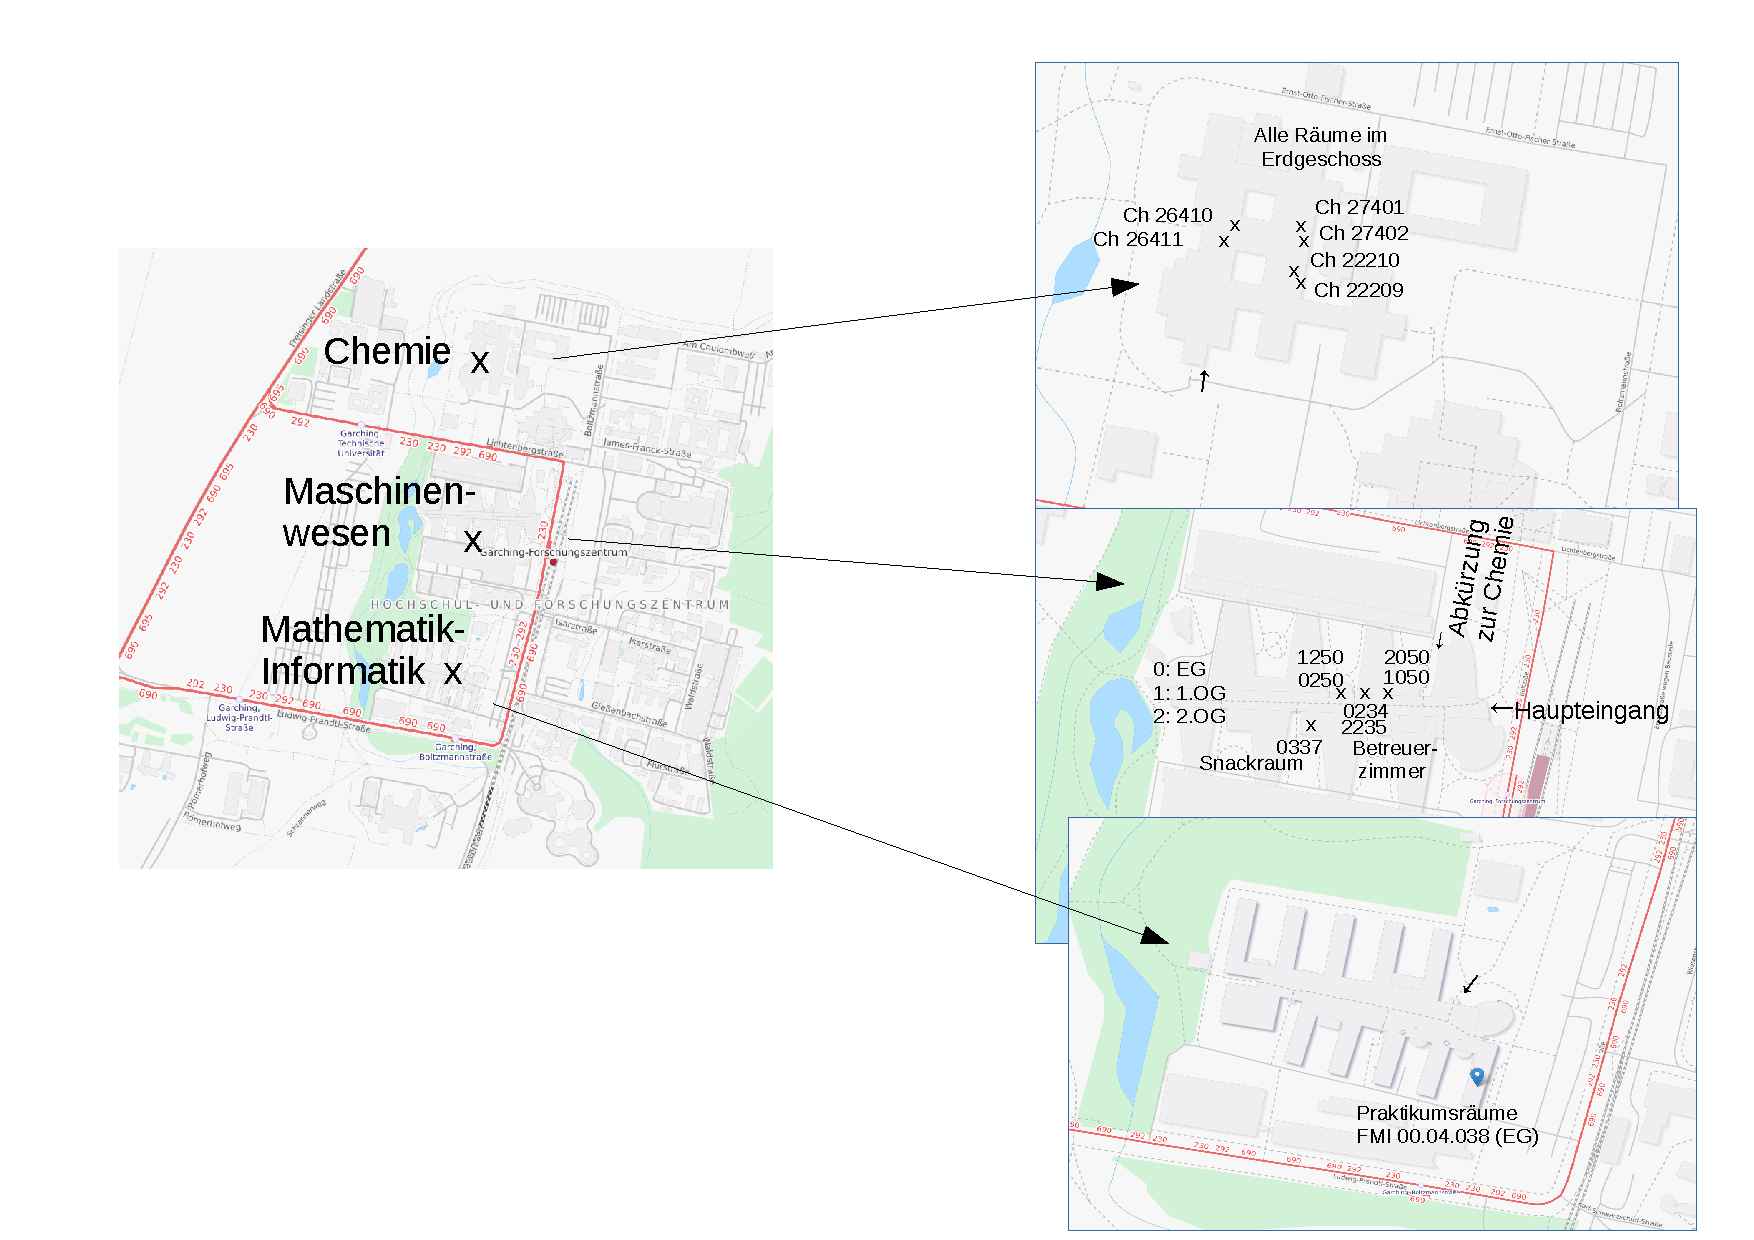
\includegraphics[scale=0.5]{campus_map.pdf}
\end{figure}
\newpage{}\begin{center}{\huge{}\textbf{Stundenplan von Lisanne Löher}}\end{center}\textbf{{\large{}Donnerstag}}\nopagebreak \\\begin{tabular} {|p{3cm} p{6cm} p{6cm}| }\hline \textbf{11:30 bis 13:45}&\textbf{Anreise zur TU München}&\textbf{Fakultät Maschinenwesen}\\\hline \textbf{12:00 bis 13:30}&\textbf{Mittagessen}&\textbf{Mensa Garching}\\\hline \textbf{14:00}&\textbf{Begrüßung}&\textbf{CH 26411}\\&Begrüßung, Besprechung des Zeitplans, Ausgabe der individuellen Stundenpläne,...&\\\hline \textbf{14:50 bis 16:20}&\textbf{Quanten- und Atomphysik I}&\textbf{CH 26410}\\&Betreuer: Ismail Achmed-Zade&ca. 28 Teilnehmer\\\hline \textbf{16:40 bis 18:10}&\textbf{Näherungsmethoden}&\textbf{MW 0234}\\&Betreuer: Ilja Göthel&ca. 13 Teilnehmer\\\hline \textbf{18:30}&\textbf{Fahrt zur Jugendherberge}&\textbf{}\\\hline \textbf{19:00}&\textbf{Abendessen}&\textbf{Jugendherberge}\\\hline \end{tabular}\\\vspace{5.00000mm}~\\\textbf{{\large{}Freitag}}\nopagebreak \\\begin{tabular} {|p{3cm} p{6cm} p{6cm}| }\hline \textbf{06:30 bis 09:00}&\textbf{Frühstück}&\textbf{Jugendherberge}\\\hline \textbf{09:00 bis 13:00}&frei&\\\hline \textbf{13:00 bis 14:00}&\textbf{Mittagessen}&\textbf{Mensa Garching}\\\hline \textbf{14:20 bis 15:50}&\textbf{Gewöhnliche Differentialgleichungen}&\textbf{MW 1250}\\&Betreuer: Sven Jandura&ca. 20 Teilnehmer\\\hline \textbf{16:10 bis 17:40}&\textbf{Spezielle Relativitätstheorie}&\textbf{MW 1250}\\&Betreuer: Johannes Rothe&ca. 19 Teilnehmer\\\hline \textbf{18:00 bis 18:20}&\textbf{Erlebnisbericht IPhO}&\textbf{CH 26411}\\\hline \textbf{18:30}&\textbf{Fahrt zur Jugendherberge}&\textbf{}\\\hline \textbf{19:00}&\textbf{Abendessen}&\textbf{Jugendherberge}\\\hline \end{tabular}\\\vspace{5.00000mm}~\\\textbf{{\large{}Samstag}}\nopagebreak \\\begin{tabular} {|p{3cm} p{6cm} p{6cm}| }\hline \textbf{06:30 bis 08:00}&\textbf{Frühstück}&\textbf{Jugendherberge}\\\hline \textbf{08:00}&\textbf{Fahrt zur TU}&\textbf{}\\\hline \textbf{09:00 bis 10:30}&\textbf{Experimentieren und Auswerten}&\textbf{CH 26411}\\&Betreuer: Ann-Kathrin Raab&ca. 18 Teilnehmer\\\hline \textbf{10:50 bis 12:20}&\textbf{Experiment Millikan-Versuch}&\textbf{Praktikum Millikan-Versuch}\\&Betreuer: Samuel Moll&ca. 6 Teilnehmer\\\hline \textbf{12:40 bis 14:00}&\textbf{Mittagessen}&\textbf{Fakultät Maschinenwesen}\\\hline \textbf{14:20 bis 15:50}&\textbf{Elektrodynamik 2}&\textbf{MW 2050}\\&Betreuer: Maximilian Keitel&ca. 6 Teilnehmer\\\hline \textbf{16:10 bis 17:40}&\textbf{Komplexe Wechselstromrechnung}&\textbf{MW 0250}\\&Betreuer: Vincent Grande&ca. 13 Teilnehmer\\\hline \textbf{18:00 bis 18:20}&\textbf{Vorstellung GYPT}&\textbf{CH 26411}\\\hline \textbf{18:30}&\textbf{Fahrt zur Jugendherberge}&\textbf{}\\\hline \textbf{19:00}&\textbf{Abendessen}&\textbf{Jugendherberge}\\\hline \end{tabular}\\\vspace{5.00000mm}~\\\textbf{{\large{}Sonntag}}\nopagebreak \\\begin{tabular} {|p{3cm} p{6cm} p{6cm}| }\hline \textbf{06:30 bis 08:00}&\textbf{Frühstück}&\textbf{Jugendherberge}\\\hline \textbf{08:00}&\textbf{Fahrt zur TU}&\textbf{}\\\hline \textbf{09:00 bis 10:30}&\textbf{Quanten- und Atomphysik II}&\textbf{MW 1250}\\&Betreuer: Vitaly Andreev&ca. 15 Teilnehmer\\\hline \textbf{10:50 bis 12:20}&\textbf{Aufgabenseminar Quanten- und Atomphysik und Struktur der Materie}&\textbf{MW 1250}\\&Betreuer: Vitaly Andreev&ca. 24 Teilnehmer\\\hline \textbf{12:40 bis 13:00}&\textbf{Verabschiedung}&\textbf{CH 26411}\\\hline \textbf{13:00}&\textbf{Individuelle Abreise}&\textbf{}\\\hline \textbf{13:00 bis 14:00}&\textbf{Mittagessen}&\textbf{}\\\hline \end{tabular}\\\vspace{5.00000mm}~\\
Notfallnummern: \\
Sven Jandura: xxxx xxxxxxxxx \\
Johannes Rothe: xxxx xxxxxxxxx \\

\large Hast du Lust, die Andern vom Seminar wiederzusehen?\\
\normalsize Dann komm doch einfach zum \textbf{Vereinstreffen}. Dazu musst du kein Vereinsmitglied sein. Neben interesannten Vorträgen und Exkursionen sind jede Menge Spiel und Spaß geplant. Schau in einem Monat einfach noch mal auf der Website vorbei. Wir freuen uns, wenn du dabei bist.

\begin{figure}[!h]
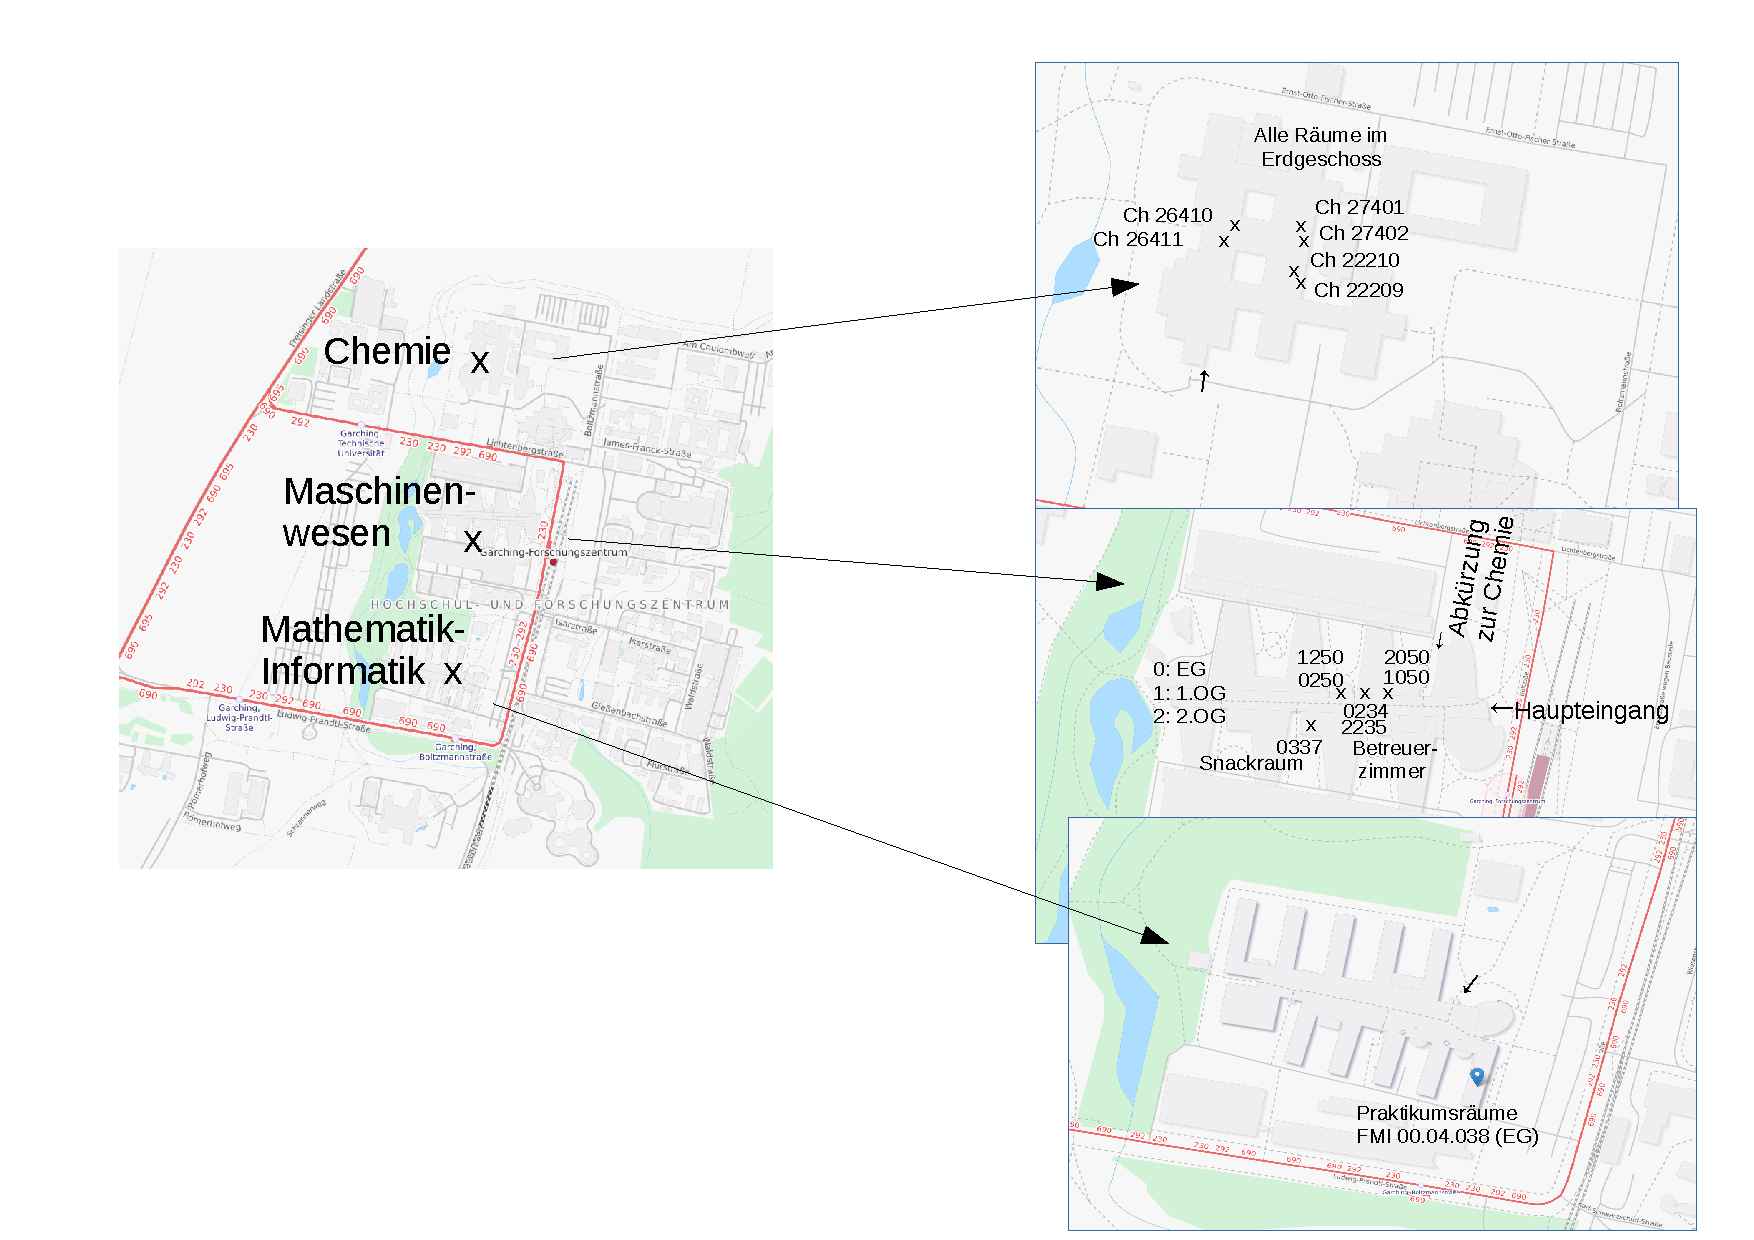
\includegraphics[scale=0.5]{campus_map.pdf}
\end{figure}
\newpage{}\begin{center}{\huge{}\textbf{Stundenplan von Lucas Kersten}}\end{center}\textbf{{\large{}Donnerstag}}\nopagebreak \\\begin{tabular} {|p{3cm} p{6cm} p{6cm}| }\hline \textbf{11:30 bis 13:45}&\textbf{Anreise zur TU München}&\textbf{Fakultät Maschinenwesen}\\\hline \textbf{12:00 bis 13:30}&\textbf{Mittagessen}&\textbf{Mensa Garching}\\\hline \textbf{14:00}&\textbf{Begrüßung}&\textbf{CH 26411}\\&Begrüßung, Besprechung des Zeitplans, Ausgabe der individuellen Stundenpläne,...&\\\hline \textbf{14:50 bis 16:20}&\textbf{Quanten- und Atomphysik I}&\textbf{CH 26410}\\&Betreuer: Ismail Achmed-Zade&ca. 28 Teilnehmer\\\hline \textbf{16:40 bis 18:10}&\textbf{Experimentieren und Auswerten}&\textbf{CH 26411}\\&Betreuer: Ann-Kathrin Raab&ca. 15 Teilnehmer\\\hline \textbf{18:30}&\textbf{Fahrt zur Jugendherberge}&\textbf{}\\\hline \textbf{19:00}&\textbf{Abendessen}&\textbf{Jugendherberge}\\\hline \end{tabular}\\\vspace{5.00000mm}~\\\textbf{{\large{}Freitag}}\nopagebreak \\\begin{tabular} {|p{3cm} p{6cm} p{6cm}| }\hline \textbf{06:30 bis 09:00}&\textbf{Frühstück}&\textbf{Jugendherberge}\\\hline \textbf{09:00 bis 13:00}&\textbf{Besichtigung der Forschungsneutronenquelle FRM II}&\textbf{MW 2050}\\&Betreuer: Felix Wechsler&ca. 28 Teilnehmer\\\hline \textbf{13:00 bis 14:00}&\textbf{Mittagessen}&\textbf{Mensa Garching}\\\hline \textbf{14:20 bis 15:50}&\textbf{Aufgabenseminar Wärmelehre}&\textbf{MW 2050}\\&Betreuer: Maximilian Marienhagen&ca. 9 Teilnehmer\\\hline \textbf{16:10 bis 17:40}&\textbf{Experiment spezifische Elektronenladung}&\textbf{Praktikum spezifische Elektronenladung}\\&Betreuer: Felix Wechsler&ca. 6 Teilnehmer\\\hline \textbf{18:00 bis 18:20}&\textbf{Erlebnisbericht IPhO}&\textbf{CH 26411}\\\hline \textbf{18:30}&\textbf{Fahrt zur Jugendherberge}&\textbf{}\\\hline \textbf{19:00}&\textbf{Abendessen}&\textbf{Jugendherberge}\\\hline \end{tabular}\\\vspace{5.00000mm}~\\\textbf{{\large{}Samstag}}\nopagebreak \\\begin{tabular} {|p{3cm} p{6cm} p{6cm}| }\hline \textbf{06:30 bis 08:00}&\textbf{Frühstück}&\textbf{Jugendherberge}\\\hline \textbf{08:00}&\textbf{Fahrt zur TU}&\textbf{}\\\hline \textbf{09:00 bis 10:30}&\textbf{Experiment Pohlsches Rad}&\textbf{Praktikum Pohlsches Rad}\\&Betreuer: Eugen Dizer&ca. 4 Teilnehmer\\\hline \textbf{10:50 bis 12:20}&\textbf{Experiment Reversionspendel}&\textbf{Praktikum Reversionspendel}\\&Betreuer: Lilith Diringer&ca. 6 Teilnehmer\\\hline \textbf{12:40 bis 14:00}&\textbf{Mittagessen}&\textbf{Fakultät Maschinenwesen}\\\hline \textbf{14:20 bis 15:50}&\textbf{Thermodynamik 1}&\textbf{MW 1250}\\&Betreuer: Maximilian Marienhagen&ca. 9 Teilnehmer\\\hline \textbf{16:10 bis 17:40}&\textbf{Himmelsmechanik}&\textbf{CH 22210}\\&Betreuer: Lars Dehlwes&ca. 10 Teilnehmer\\\hline \textbf{18:00 bis 18:20}&\textbf{Vorstellung GYPT}&\textbf{CH 26411}\\\hline \textbf{18:30}&\textbf{Fahrt zur Jugendherberge}&\textbf{}\\\hline \textbf{19:00}&\textbf{Abendessen}&\textbf{Jugendherberge}\\\hline \end{tabular}\\\vspace{5.00000mm}~\\\textbf{{\large{}Sonntag}}\nopagebreak \\\begin{tabular} {|p{3cm} p{6cm} p{6cm}| }\hline \textbf{06:30 bis 08:00}&\textbf{Frühstück}&\textbf{Jugendherberge}\\\hline \textbf{08:00}&\textbf{Fahrt zur TU}&\textbf{}\\\hline \textbf{09:00 bis 10:30}&\textbf{Theoretische Mechanik}&\textbf{CH 22210}\\&Betreuer: Eugen Dizer&ca. 13 Teilnehmer\\\hline \textbf{10:50 bis 12:20}&\textbf{Rotationsbewegungen}&\textbf{CH 26410}\\&Betreuer: Vincent Grande&ca. 9 Teilnehmer\\\hline \textbf{12:40 bis 13:00}&\textbf{Verabschiedung}&\textbf{CH 26411}\\\hline \textbf{13:00}&\textbf{Individuelle Abreise}&\textbf{}\\\hline \textbf{13:00 bis 14:00}&\textbf{Mittagessen}&\textbf{}\\\hline \end{tabular}\\\vspace{5.00000mm}~\\
Notfallnummern: \\
Sven Jandura: xxxx xxxxxxxxx \\
Johannes Rothe: xxxx xxxxxxxxx \\

\large Hast du Lust, die Andern vom Seminar wiederzusehen?\\
\normalsize Dann komm doch einfach zum \textbf{Vereinstreffen}. Dazu musst du kein Vereinsmitglied sein. Neben interesannten Vorträgen und Exkursionen sind jede Menge Spiel und Spaß geplant. Schau in einem Monat einfach noch mal auf der Website vorbei. Wir freuen uns, wenn du dabei bist.

\begin{figure}[!h]
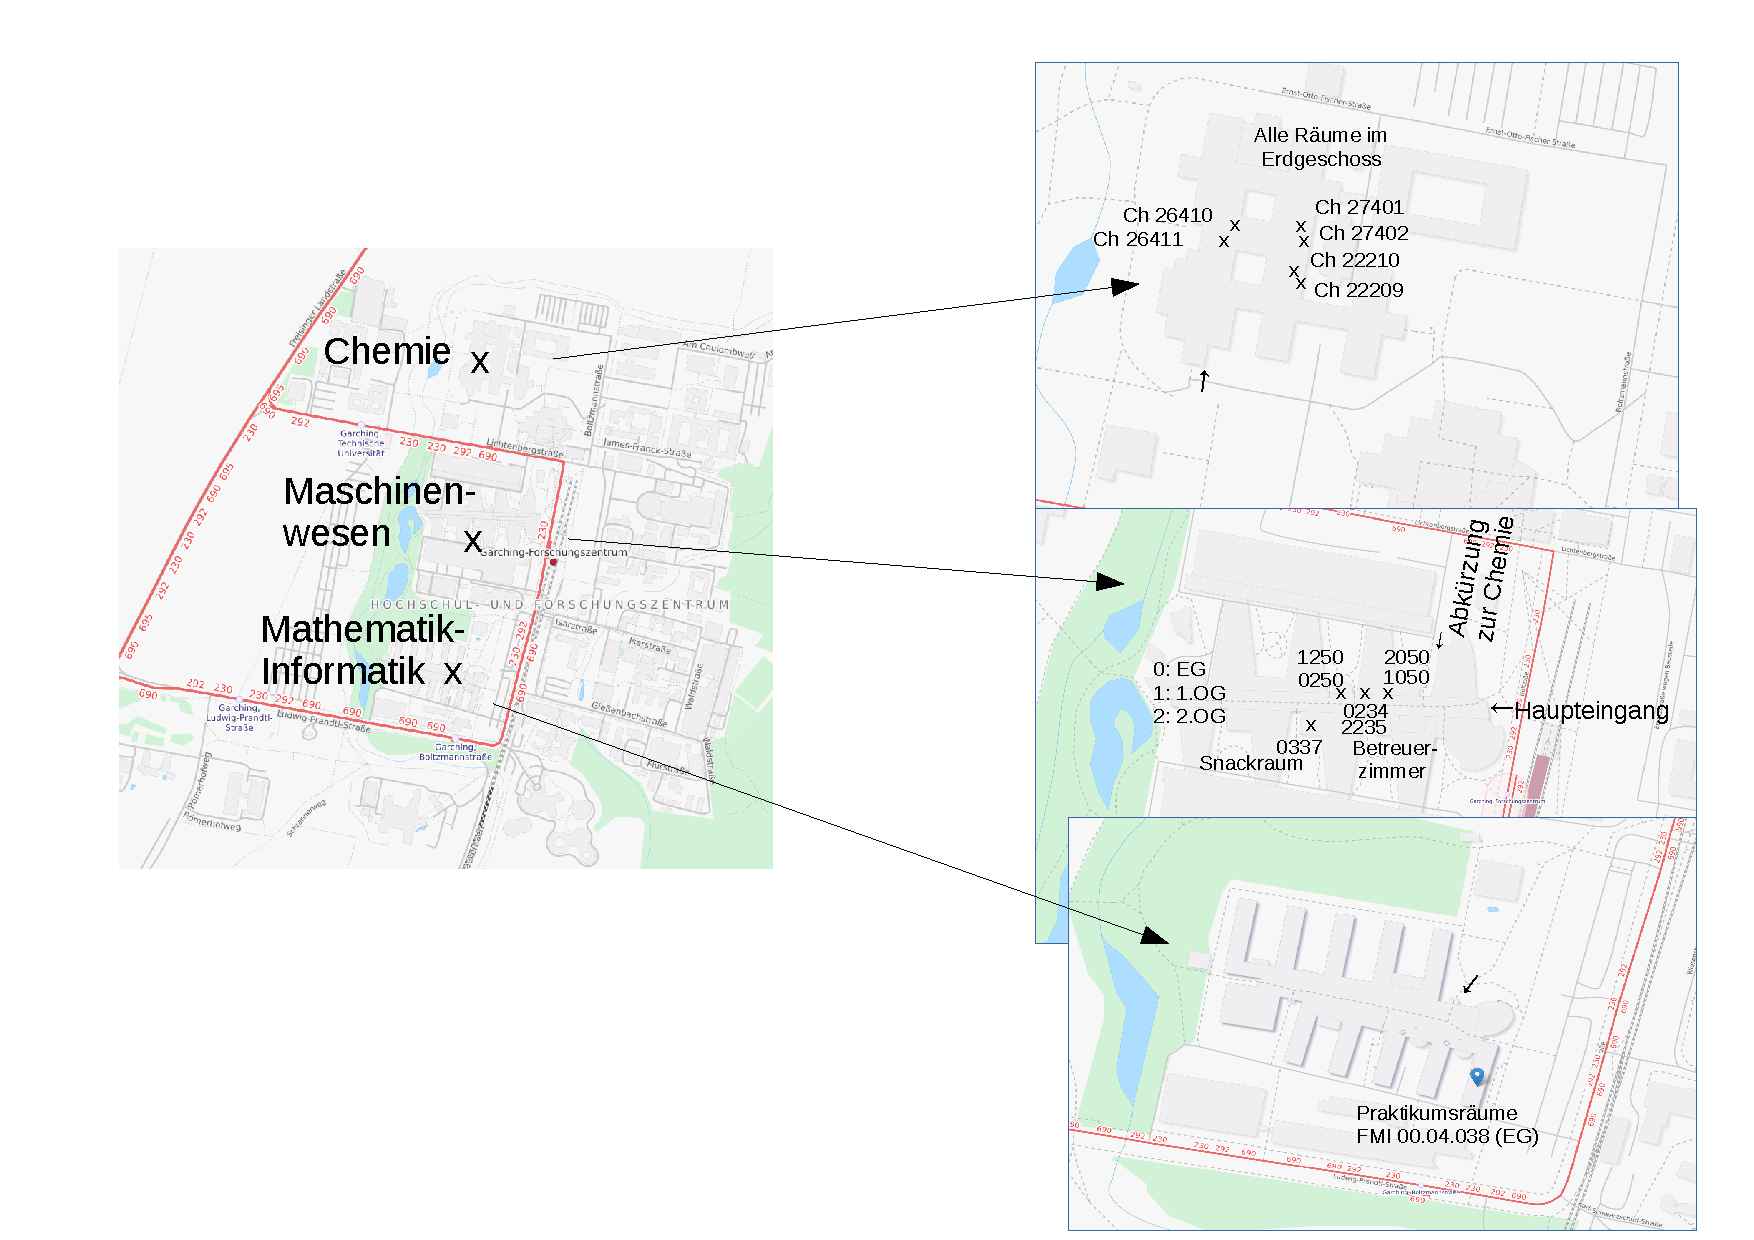
\includegraphics[scale=0.5]{campus_map.pdf}
\end{figure}
\newpage{}\begin{center}{\huge{}\textbf{Stundenplan von Lucas Reisener}}\end{center}\textbf{{\large{}Donnerstag}}\nopagebreak \\\begin{tabular} {|p{3cm} p{6cm} p{6cm}| }\hline \textbf{11:30 bis 13:45}&\textbf{Anreise zur TU München}&\textbf{Fakultät Maschinenwesen}\\\hline \textbf{12:00 bis 13:30}&\textbf{Mittagessen}&\textbf{Mensa Garching}\\\hline \textbf{14:00}&\textbf{Begrüßung}&\textbf{CH 26411}\\&Begrüßung, Besprechung des Zeitplans, Ausgabe der individuellen Stundenpläne,...&\\\hline \textbf{14:50 bis 16:20}&frei&\\\hline \textbf{16:40 bis 18:10}&frei&\\\hline \textbf{18:30}&\textbf{Fahrt zur Jugendherberge}&\textbf{}\\\hline \textbf{19:00}&\textbf{Abendessen}&\textbf{Jugendherberge}\\\hline \end{tabular}\\\vspace{5.00000mm}~\\\textbf{{\large{}Freitag}}\nopagebreak \\\begin{tabular} {|p{3cm} p{6cm} p{6cm}| }\hline \textbf{06:30 bis 09:00}&\textbf{Frühstück}&\textbf{Jugendherberge}\\\hline \textbf{09:00 bis 13:00}&frei&\\\hline \textbf{13:00 bis 14:00}&\textbf{Mittagessen}&\textbf{Mensa Garching}\\\hline \textbf{14:20 bis 15:50}&frei&\\\hline \textbf{16:10 bis 17:40}&frei&\\\hline \textbf{18:00 bis 18:20}&\textbf{Erlebnisbericht IPhO}&\textbf{CH 26411}\\\hline \textbf{18:30}&\textbf{Fahrt zur Jugendherberge}&\textbf{}\\\hline \textbf{19:00}&\textbf{Abendessen}&\textbf{Jugendherberge}\\\hline \end{tabular}\\\vspace{5.00000mm}~\\\textbf{{\large{}Samstag}}\nopagebreak \\\begin{tabular} {|p{3cm} p{6cm} p{6cm}| }\hline \textbf{06:30 bis 08:00}&\textbf{Frühstück}&\textbf{Jugendherberge}\\\hline \textbf{08:00}&\textbf{Fahrt zur TU}&\textbf{}\\\hline \textbf{09:00 bis 10:30}&\textbf{Experiment Brennstoffzelle}&\textbf{Praktikum Brennstoffzelle}\\&Betreuer: Aaron Wild&ca. 6 Teilnehmer\\\hline \textbf{10:50 bis 12:20}&\textbf{Experiment Reversionspendel}&\textbf{Praktikum Reversionspendel}\\&Betreuer: Lilith Diringer&ca. 6 Teilnehmer\\\hline \textbf{12:40 bis 14:00}&\textbf{Mittagessen}&\textbf{Fakultät Maschinenwesen}\\\hline \textbf{14:20 bis 15:50}&\textbf{Quanten- und Atomphysik I}&\textbf{CH 22209}\\&Betreuer: Vitaly Andreev&ca. 22 Teilnehmer\\\hline \textbf{16:10 bis 17:40}&frei&\\\hline \textbf{18:00 bis 18:20}&\textbf{Vorstellung GYPT}&\textbf{CH 26411}\\\hline \textbf{18:30}&\textbf{Fahrt zur Jugendherberge}&\textbf{}\\\hline \textbf{19:00}&\textbf{Abendessen}&\textbf{Jugendherberge}\\\hline \end{tabular}\\\vspace{5.00000mm}~\\\textbf{{\large{}Sonntag}}\nopagebreak \\\begin{tabular} {|p{3cm} p{6cm} p{6cm}| }\hline \textbf{06:30 bis 08:00}&\textbf{Frühstück}&\textbf{Jugendherberge}\\\hline \textbf{08:00}&\textbf{Fahrt zur TU}&\textbf{}\\\hline \textbf{09:00 bis 10:30}&frei&\\\hline \textbf{10:50 bis 12:20}&\textbf{Bestimmung des Brechungskoeffizienten von Plexiglas}&\textbf{MW 0234}\\&Betreuer: Lilith Diringer&ca. 8 Teilnehmer\\\hline \textbf{12:40 bis 13:00}&\textbf{Verabschiedung}&\textbf{CH 26411}\\\hline \textbf{13:00}&\textbf{Individuelle Abreise}&\textbf{}\\\hline \textbf{13:00 bis 14:00}&\textbf{Mittagessen}&\textbf{}\\\hline \end{tabular}\\\vspace{5.00000mm}~\\
Notfallnummern: \\
Sven Jandura: xxxx xxxxxxxxx \\
Johannes Rothe: xxxx xxxxxxxxx \\

\large Hast du Lust, die Andern vom Seminar wiederzusehen?\\
\normalsize Dann komm doch einfach zum \textbf{Vereinstreffen}. Dazu musst du kein Vereinsmitglied sein. Neben interesannten Vorträgen und Exkursionen sind jede Menge Spiel und Spaß geplant. Schau in einem Monat einfach noch mal auf der Website vorbei. Wir freuen uns, wenn du dabei bist.

\begin{figure}[!h]
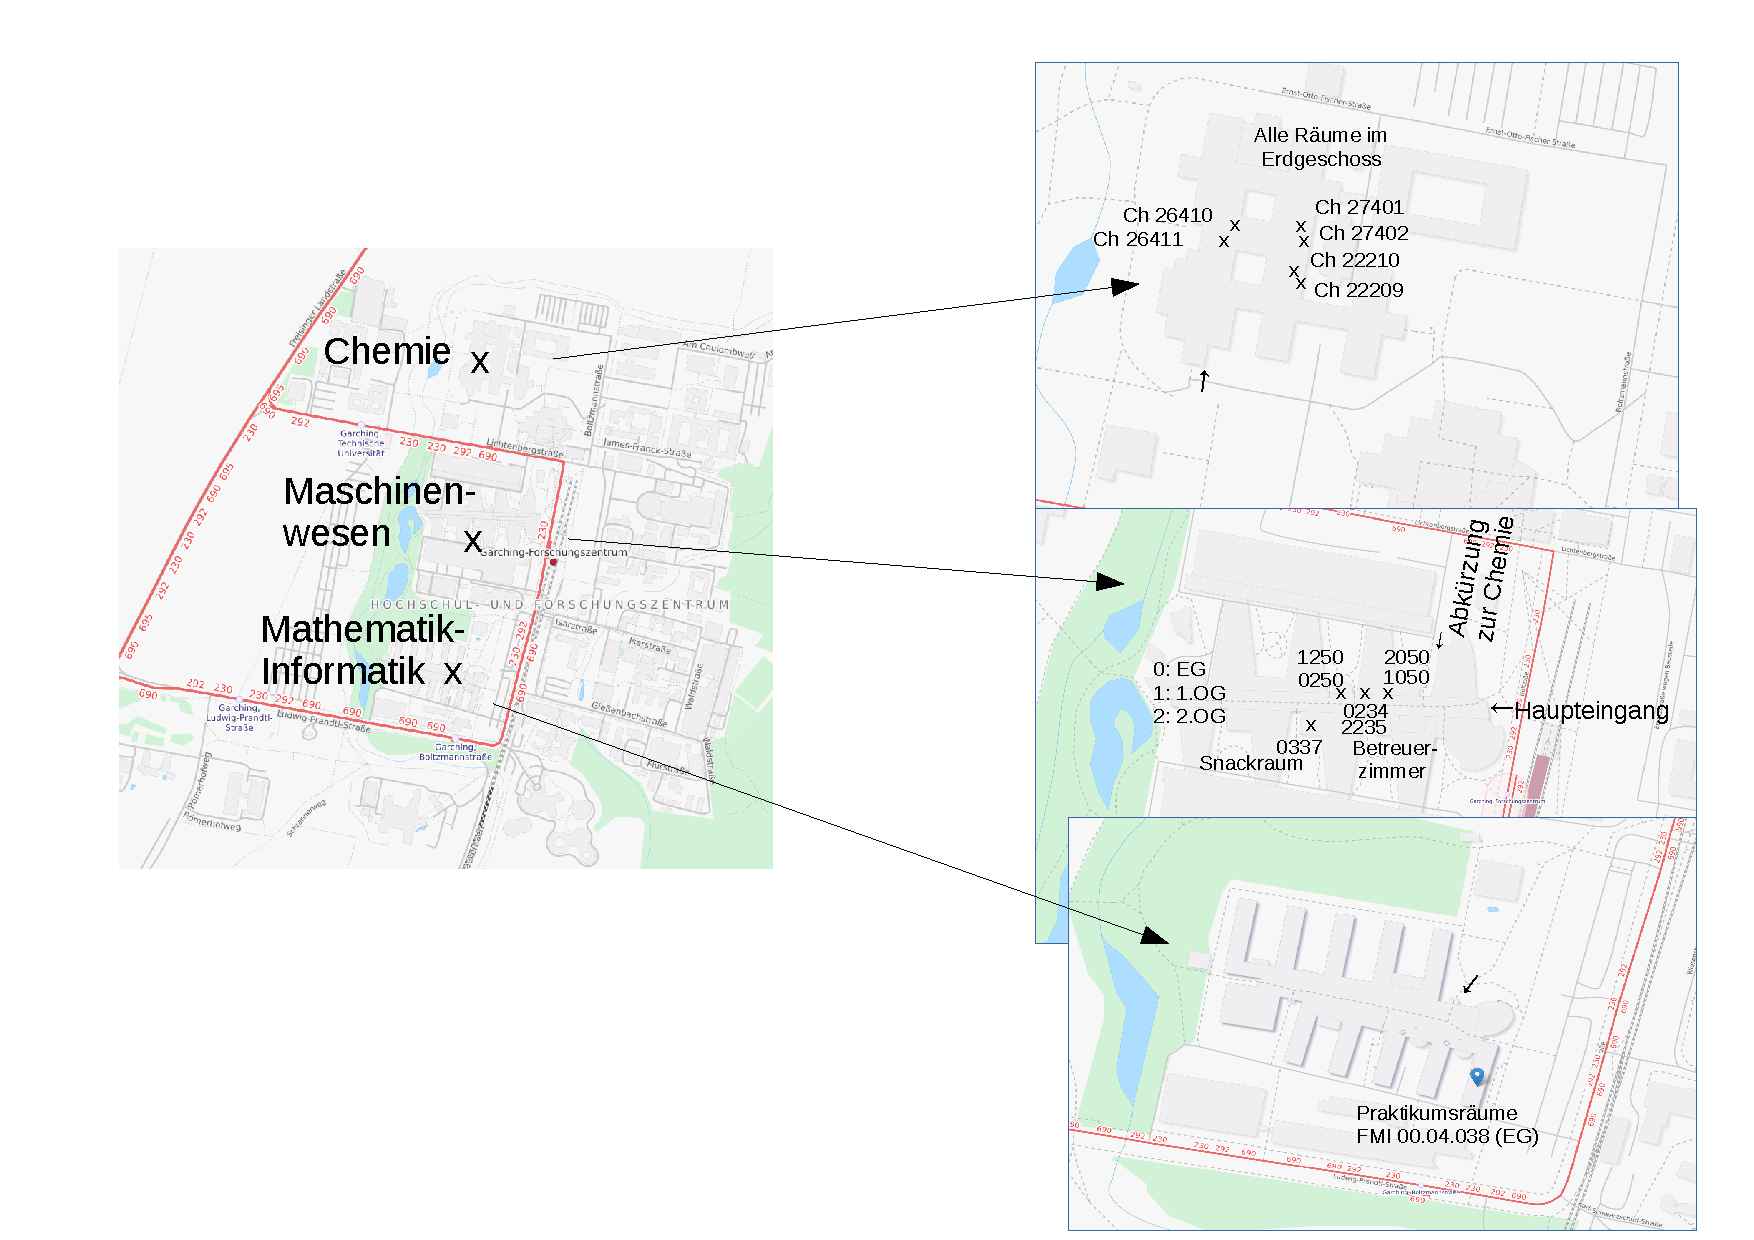
\includegraphics[scale=0.5]{campus_map.pdf}
\end{figure}
\newpage{}\begin{center}{\huge{}\textbf{Stundenplan von Lukas Eberhardt}}\end{center}\textbf{{\large{}Donnerstag}}\nopagebreak \\\begin{tabular} {|p{3cm} p{6cm} p{6cm}| }\hline \textbf{11:30 bis 13:45}&\textbf{Anreise zur TU München}&\textbf{Fakultät Maschinenwesen}\\\hline \textbf{12:00 bis 13:30}&\textbf{Mittagessen}&\textbf{Mensa Garching}\\\hline \textbf{14:00}&\textbf{Begrüßung}&\textbf{CH 26411}\\&Begrüßung, Besprechung des Zeitplans, Ausgabe der individuellen Stundenpläne,...&\\\hline \textbf{14:50 bis 16:20}&\textbf{Spezielle Funktionen und Vektorrechnung}&\textbf{MW 0234}\\&Betreuer: Lilith Diringer&ca. 4 Teilnehmer\\\hline \textbf{16:40 bis 18:10}&\textbf{Experimentieren und Auswerten}&\textbf{CH 26411}\\&Betreuer: Ann-Kathrin Raab&ca. 15 Teilnehmer\\\hline \textbf{18:30}&\textbf{Fahrt zur Jugendherberge}&\textbf{}\\\hline \textbf{19:00}&\textbf{Abendessen}&\textbf{Jugendherberge}\\\hline \end{tabular}\\\vspace{5.00000mm}~\\\textbf{{\large{}Freitag}}\nopagebreak \\\begin{tabular} {|p{3cm} p{6cm} p{6cm}| }\hline \textbf{06:30 bis 09:00}&\textbf{Frühstück}&\textbf{Jugendherberge}\\\hline \textbf{09:00 bis 13:00}&frei&\\\hline \textbf{13:00 bis 14:00}&\textbf{Mittagessen}&\textbf{Mensa Garching}\\\hline \textbf{14:20 bis 15:50}&\textbf{Experiment Oszilloskop}&\textbf{Praktikum Oszilloskop}\\&Betreuer: Christopher Pfeiffer&ca. 6 Teilnehmer\\\hline \textbf{16:10 bis 17:40}&\textbf{Experiment Brückenschaltung}&\textbf{Praktikum Brückenschaltung}\\&Betreuer: Martin Großhauser&ca. 6 Teilnehmer\\\hline \textbf{18:00 bis 18:20}&\textbf{Erlebnisbericht IPhO}&\textbf{CH 26411}\\\hline \textbf{18:30}&\textbf{Fahrt zur Jugendherberge}&\textbf{}\\\hline \textbf{19:00}&\textbf{Abendessen}&\textbf{Jugendherberge}\\\hline \end{tabular}\\\vspace{5.00000mm}~\\\textbf{{\large{}Samstag}}\nopagebreak \\\begin{tabular} {|p{3cm} p{6cm} p{6cm}| }\hline \textbf{06:30 bis 08:00}&\textbf{Frühstück}&\textbf{Jugendherberge}\\\hline \textbf{08:00}&\textbf{Fahrt zur TU}&\textbf{}\\\hline \textbf{09:00 bis 10:30}&\textbf{Experiment Pohlsches Rad}&\textbf{Praktikum Pohlsches Rad}\\&Betreuer: Eugen Dizer&ca. 4 Teilnehmer\\\hline \textbf{10:50 bis 12:20}&\textbf{Experiment Reversionspendel}&\textbf{Praktikum Reversionspendel}\\&Betreuer: Lilith Diringer&ca. 6 Teilnehmer\\\hline \textbf{12:40 bis 14:00}&\textbf{Mittagessen}&\textbf{Fakultät Maschinenwesen}\\\hline \textbf{14:20 bis 15:50}&\textbf{Elektrische Schaltungen}&\textbf{CH 26410}\\&Betreuer: Felix Wechsler&ca. 4 Teilnehmer\\\hline \textbf{16:10 bis 17:40}&\textbf{Elektrische Blackboxen}&\textbf{Praktikum Blackboxen}\\&Betreuer: Eugen Dizer&ca. 6 Teilnehmer\\\hline \textbf{18:00 bis 18:20}&\textbf{Vorstellung GYPT}&\textbf{CH 26411}\\\hline \textbf{18:30}&\textbf{Fahrt zur Jugendherberge}&\textbf{}\\\hline \textbf{19:00}&\textbf{Abendessen}&\textbf{Jugendherberge}\\\hline \end{tabular}\\\vspace{5.00000mm}~\\\textbf{{\large{}Sonntag}}\nopagebreak \\\begin{tabular} {|p{3cm} p{6cm} p{6cm}| }\hline \textbf{06:30 bis 08:00}&\textbf{Frühstück}&\textbf{Jugendherberge}\\\hline \textbf{08:00}&\textbf{Fahrt zur TU}&\textbf{}\\\hline \textbf{09:00 bis 10:30}&\textbf{Elektronik}&\textbf{CH 26410}\\&Betreuer: Martin Großhauser&ca. 10 Teilnehmer\\\hline \textbf{10:50 bis 12:20}&\textbf{Wellenoptik}&\textbf{MW 0250}\\&Betreuer: Christopher Pfeiffer&ca. 12 Teilnehmer\\\hline \textbf{12:40 bis 13:00}&\textbf{Verabschiedung}&\textbf{CH 26411}\\\hline \textbf{13:00}&\textbf{Individuelle Abreise}&\textbf{}\\\hline \textbf{13:00 bis 14:00}&\textbf{Mittagessen}&\textbf{}\\\hline \end{tabular}\\\vspace{5.00000mm}~\\
Notfallnummern: \\
Sven Jandura: xxxx xxxxxxxxx \\
Johannes Rothe: xxxx xxxxxxxxx \\

\large Hast du Lust, die Andern vom Seminar wiederzusehen?\\
\normalsize Dann komm doch einfach zum \textbf{Vereinstreffen}. Dazu musst du kein Vereinsmitglied sein. Neben interesannten Vorträgen und Exkursionen sind jede Menge Spiel und Spaß geplant. Schau in einem Monat einfach noch mal auf der Website vorbei. Wir freuen uns, wenn du dabei bist.

\begin{figure}[!h]
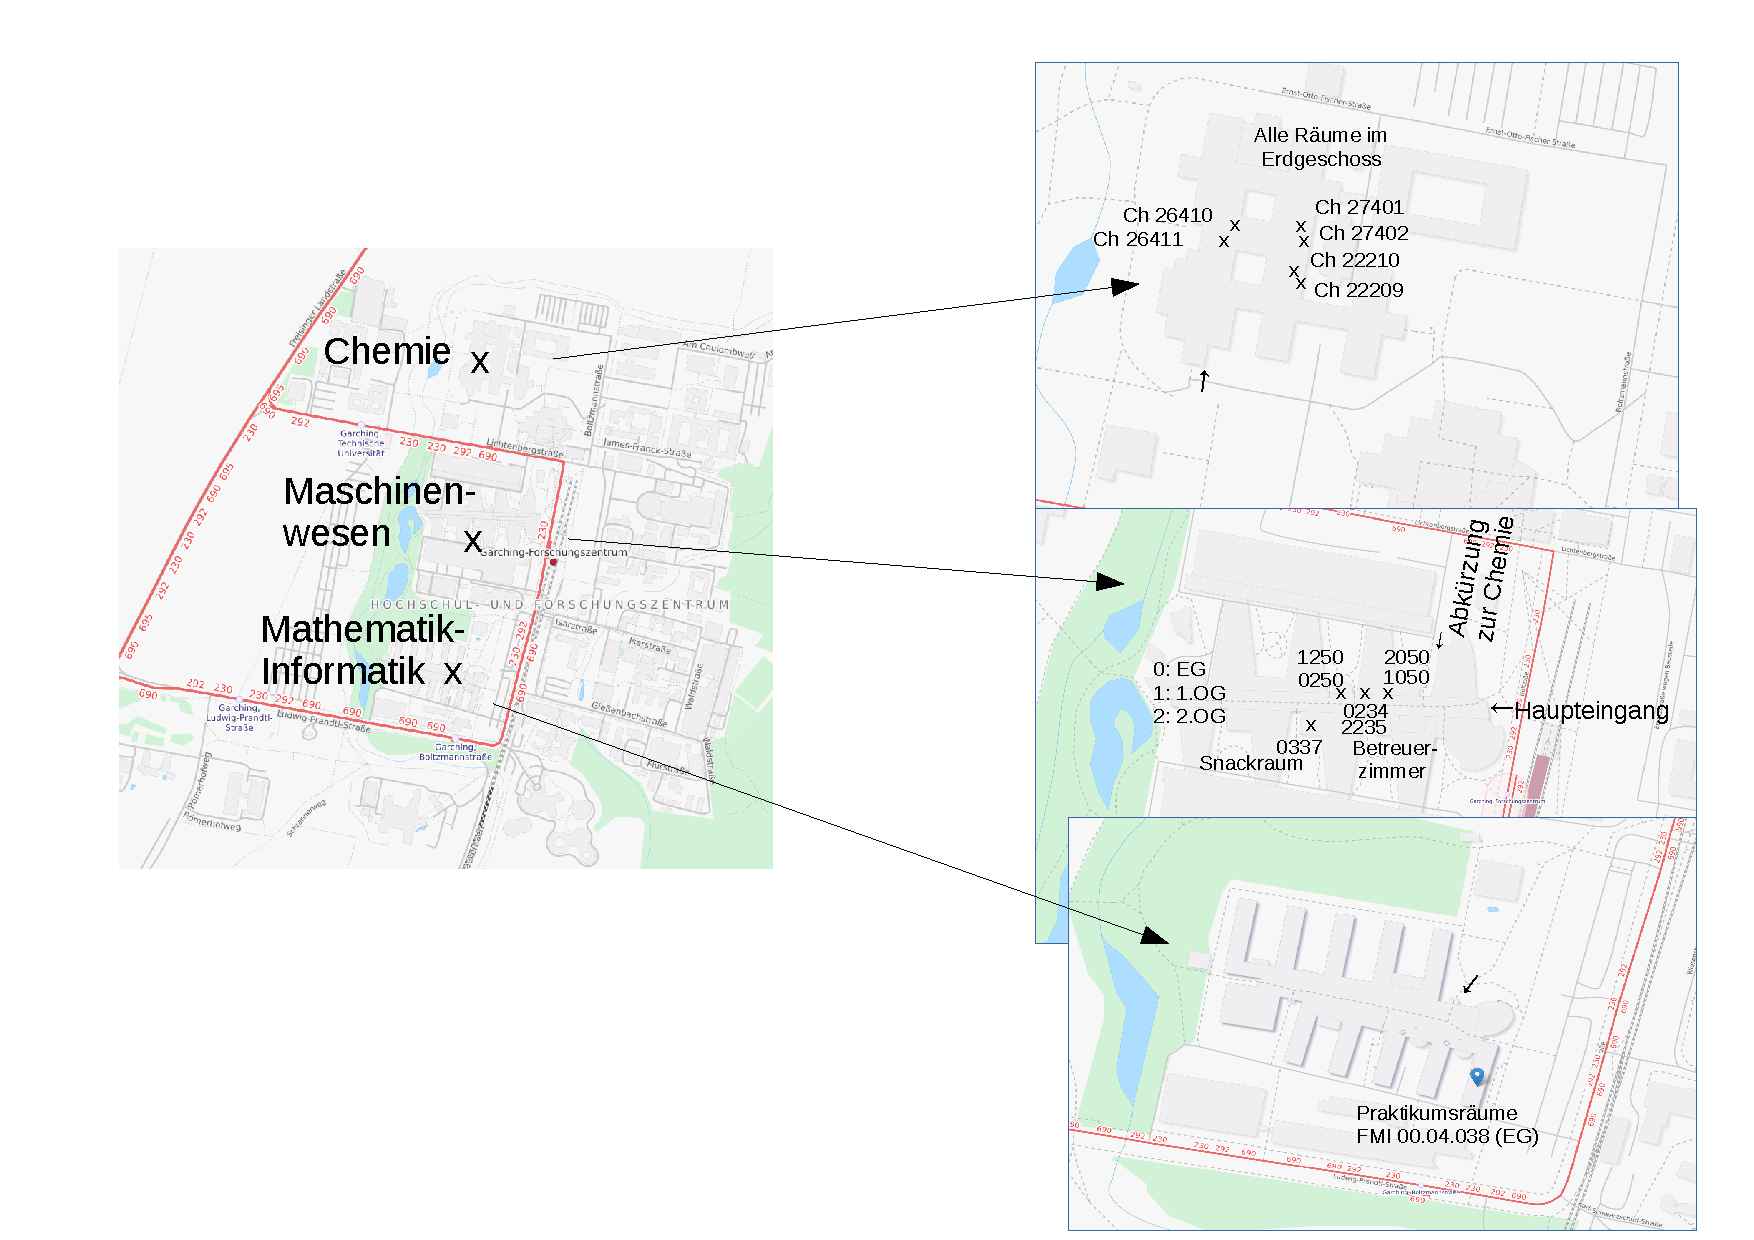
\includegraphics[scale=0.5]{campus_map.pdf}
\end{figure}
\newpage{}\begin{center}{\huge{}\textbf{Stundenplan von Lukas Schulz}}\end{center}\textbf{{\large{}Donnerstag}}\nopagebreak \\\begin{tabular} {|p{3cm} p{6cm} p{6cm}| }\hline \textbf{11:30 bis 13:45}&\textbf{Anreise zur TU München}&\textbf{Fakultät Maschinenwesen}\\\hline \textbf{12:00 bis 13:30}&\textbf{Mittagessen}&\textbf{Mensa Garching}\\\hline \textbf{14:00}&\textbf{Begrüßung}&\textbf{CH 26411}\\&Begrüßung, Besprechung des Zeitplans, Ausgabe der individuellen Stundenpläne,...&\\\hline \textbf{14:50 bis 16:20}&\textbf{Elektrische Schaltungen}&\textbf{MW 0250}\\&Betreuer: Christopher Pfeiffer&ca. 16 Teilnehmer\\\hline \textbf{16:40 bis 18:10}&\textbf{Geometrische Optik}&\textbf{MW 0250}\\&Betreuer: Christopher Pfeiffer&ca. 13 Teilnehmer\\\hline \textbf{18:30}&\textbf{Fahrt zur Jugendherberge}&\textbf{}\\\hline \textbf{19:00}&\textbf{Abendessen}&\textbf{Jugendherberge}\\\hline \end{tabular}\\\vspace{5.00000mm}~\\\textbf{{\large{}Freitag}}\nopagebreak \\\begin{tabular} {|p{3cm} p{6cm} p{6cm}| }\hline \textbf{06:30 bis 09:00}&\textbf{Frühstück}&\textbf{Jugendherberge}\\\hline \textbf{09:00 bis 13:00}&\textbf{Besichtigung der Forschungsneutronenquelle FRM II}&\textbf{MW 2050}\\&Betreuer: Felix Wechsler&ca. 28 Teilnehmer\\\hline \textbf{13:00 bis 14:00}&\textbf{Mittagessen}&\textbf{Mensa Garching}\\\hline \textbf{14:20 bis 15:50}&\textbf{Spezielle Funktionen und Vektorrechnung}&\textbf{MW 0234}\\&Betreuer: Lilith Diringer&ca. 3 Teilnehmer\\\hline \textbf{16:10 bis 17:40}&\textbf{Einführung ins Integrieren}&\textbf{MW 2050}\\&Betreuer: Felix Wechsler&ca. 14 Teilnehmer\\\hline \textbf{18:00 bis 18:20}&\textbf{Erlebnisbericht IPhO}&\textbf{CH 26411}\\\hline \textbf{18:30}&\textbf{Fahrt zur Jugendherberge}&\textbf{}\\\hline \textbf{19:00}&\textbf{Abendessen}&\textbf{Jugendherberge}\\\hline \end{tabular}\\\vspace{5.00000mm}~\\\textbf{{\large{}Samstag}}\nopagebreak \\\begin{tabular} {|p{3cm} p{6cm} p{6cm}| }\hline \textbf{06:30 bis 08:00}&\textbf{Frühstück}&\textbf{Jugendherberge}\\\hline \textbf{08:00}&\textbf{Fahrt zur TU}&\textbf{}\\\hline \textbf{09:00 bis 10:30}&\textbf{Elektrodynamik 1}&\textbf{MW 1250}\\&Betreuer: Maximilian Keitel&ca. 21 Teilnehmer\\\hline \textbf{10:50 bis 12:20}&\textbf{Elektrodynamik 2}&\textbf{MW 1250}\\&Betreuer: Maximilian Keitel&ca. 21 Teilnehmer\\\hline \textbf{12:40 bis 14:00}&\textbf{Mittagessen}&\textbf{Fakultät Maschinenwesen}\\\hline \textbf{14:20 bis 15:50}&\textbf{Quanten- und Atomphysik I}&\textbf{CH 22209}\\&Betreuer: Vitaly Andreev&ca. 22 Teilnehmer\\\hline \textbf{16:10 bis 17:40}&\textbf{Komplexe Wechselstromrechnung}&\textbf{MW 0250}\\&Betreuer: Vincent Grande&ca. 13 Teilnehmer\\\hline \textbf{18:00 bis 18:20}&\textbf{Vorstellung GYPT}&\textbf{CH 26411}\\\hline \textbf{18:30}&\textbf{Fahrt zur Jugendherberge}&\textbf{}\\\hline \textbf{19:00}&\textbf{Abendessen}&\textbf{Jugendherberge}\\\hline \end{tabular}\\\vspace{5.00000mm}~\\\textbf{{\large{}Sonntag}}\nopagebreak \\\begin{tabular} {|p{3cm} p{6cm} p{6cm}| }\hline \textbf{06:30 bis 08:00}&\textbf{Frühstück}&\textbf{Jugendherberge}\\\hline \textbf{08:00}&\textbf{Fahrt zur TU}&\textbf{}\\\hline \textbf{09:00 bis 10:30}&\textbf{Spezielle Relativitätstheorie}&\textbf{MW 0250}\\&Betreuer: Johannes Rothe&ca. 12 Teilnehmer\\\hline \textbf{10:50 bis 12:20}&\textbf{Aufgabenseminar Quanten- und Atomphysik und Struktur der Materie}&\textbf{MW 1250}\\&Betreuer: Vitaly Andreev&ca. 24 Teilnehmer\\\hline \textbf{12:40 bis 13:00}&\textbf{Verabschiedung}&\textbf{CH 26411}\\\hline \textbf{13:00}&\textbf{Individuelle Abreise}&\textbf{}\\\hline \textbf{13:00 bis 14:00}&\textbf{Mittagessen}&\textbf{}\\\hline \end{tabular}\\\vspace{5.00000mm}~\\
Notfallnummern: \\
Sven Jandura: xxxx xxxxxxxxx \\
Johannes Rothe: xxxx xxxxxxxxx \\

\large Hast du Lust, die Andern vom Seminar wiederzusehen?\\
\normalsize Dann komm doch einfach zum \textbf{Vereinstreffen}. Dazu musst du kein Vereinsmitglied sein. Neben interesannten Vorträgen und Exkursionen sind jede Menge Spiel und Spaß geplant. Schau in einem Monat einfach noch mal auf der Website vorbei. Wir freuen uns, wenn du dabei bist.

\begin{figure}[!h]
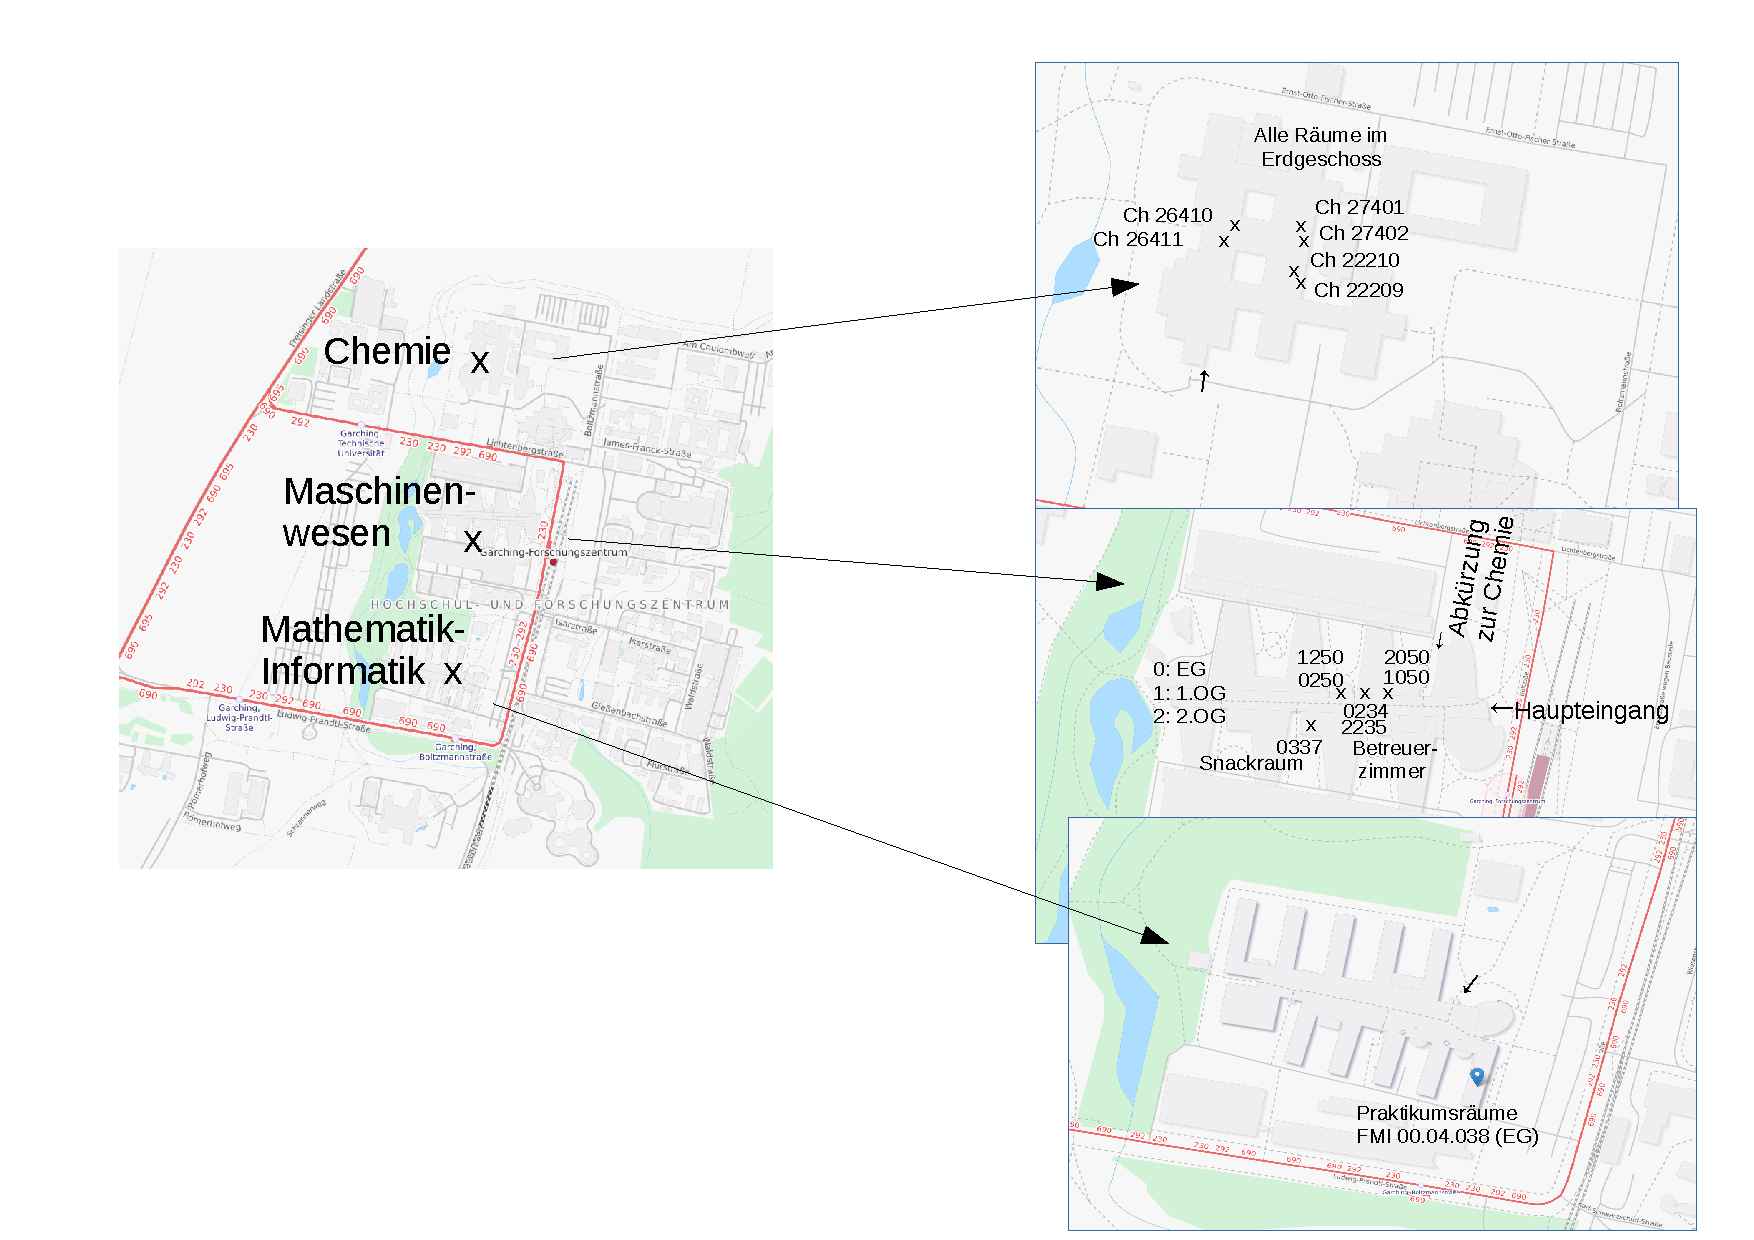
\includegraphics[scale=0.5]{campus_map.pdf}
\end{figure}
\newpage{}\begin{center}{\huge{}\textbf{Stundenplan von Lukas  Grünwald}}\end{center}\textbf{{\large{}Donnerstag}}\nopagebreak \\\begin{tabular} {|p{3cm} p{6cm} p{6cm}| }\hline \textbf{11:30 bis 13:45}&\textbf{Anreise zur TU München}&\textbf{Fakultät Maschinenwesen}\\\hline \textbf{12:00 bis 13:30}&\textbf{Mittagessen}&\textbf{Mensa Garching}\\\hline \textbf{14:00}&\textbf{Begrüßung}&\textbf{CH 26411}\\&Begrüßung, Besprechung des Zeitplans, Ausgabe der individuellen Stundenpläne,...&\\\hline \textbf{14:50 bis 16:20}&\textbf{Quanten- und Atomphysik I}&\textbf{CH 26410}\\&Betreuer: Ismail Achmed-Zade&ca. 28 Teilnehmer\\\hline \textbf{16:40 bis 18:10}&\textbf{Einführung ins Integrieren}&\textbf{MW 1050}\\&Betreuer: Johannes Rothe&ca. 14 Teilnehmer\\\hline \textbf{18:30}&\textbf{Fahrt zur Jugendherberge}&\textbf{}\\\hline \textbf{19:00}&\textbf{Abendessen}&\textbf{Jugendherberge}\\\hline \end{tabular}\\\vspace{5.00000mm}~\\\textbf{{\large{}Freitag}}\nopagebreak \\\begin{tabular} {|p{3cm} p{6cm} p{6cm}| }\hline \textbf{06:30 bis 09:00}&\textbf{Frühstück}&\textbf{Jugendherberge}\\\hline \textbf{09:00 bis 13:00}&frei&\\\hline \textbf{13:00 bis 14:00}&\textbf{Mittagessen}&\textbf{Mensa Garching}\\\hline \textbf{14:20 bis 15:50}&\textbf{Kernphysik}&\textbf{MW 0250}\\&Betreuer: Johannes Rothe&ca. 18 Teilnehmer\\\hline \textbf{16:10 bis 17:40}&\textbf{Spezielle Relativitätstheorie}&\textbf{MW 1250}\\&Betreuer: Johannes Rothe&ca. 19 Teilnehmer\\\hline \textbf{18:00 bis 18:20}&\textbf{Erlebnisbericht IPhO}&\textbf{CH 26411}\\\hline \textbf{18:30}&\textbf{Fahrt zur Jugendherberge}&\textbf{}\\\hline \textbf{19:00}&\textbf{Abendessen}&\textbf{Jugendherberge}\\\hline \end{tabular}\\\vspace{5.00000mm}~\\\textbf{{\large{}Samstag}}\nopagebreak \\\begin{tabular} {|p{3cm} p{6cm} p{6cm}| }\hline \textbf{06:30 bis 08:00}&\textbf{Frühstück}&\textbf{Jugendherberge}\\\hline \textbf{08:00}&\textbf{Fahrt zur TU}&\textbf{}\\\hline \textbf{09:00 bis 10:30}&\textbf{Experimentieren und Auswerten}&\textbf{CH 26411}\\&Betreuer: Ann-Kathrin Raab&ca. 18 Teilnehmer\\\hline \textbf{10:50 bis 12:20}&\textbf{Elektrodynamik 2}&\textbf{MW 1250}\\&Betreuer: Maximilian Keitel&ca. 21 Teilnehmer\\\hline \textbf{12:40 bis 14:00}&\textbf{Mittagessen}&\textbf{Fakultät Maschinenwesen}\\\hline \textbf{14:20 bis 15:50}&\textbf{Gravitationsbeschleunigung}&\textbf{MW 1050}\\&Betreuer: Ann-Kathrin Raab&ca. 8 Teilnehmer\\\hline \textbf{16:10 bis 17:40}&\textbf{Aufgabenseminar Elektrodynamik}&\textbf{MW 1250}\\&Betreuer: Maximilian Keitel&ca. 8 Teilnehmer\\\hline \textbf{18:00 bis 18:20}&\textbf{Vorstellung GYPT}&\textbf{CH 26411}\\\hline \textbf{18:30}&\textbf{Fahrt zur Jugendherberge}&\textbf{}\\\hline \textbf{19:00}&\textbf{Abendessen}&\textbf{Jugendherberge}\\\hline \end{tabular}\\\vspace{5.00000mm}~\\\textbf{{\large{}Sonntag}}\nopagebreak \\\begin{tabular} {|p{3cm} p{6cm} p{6cm}| }\hline \textbf{06:30 bis 08:00}&\textbf{Frühstück}&\textbf{Jugendherberge}\\\hline \textbf{08:00}&\textbf{Fahrt zur TU}&\textbf{}\\\hline \textbf{09:00 bis 10:30}&\textbf{Quanten- und Atomphysik II}&\textbf{MW 1250}\\&Betreuer: Vitaly Andreev&ca. 15 Teilnehmer\\\hline \textbf{10:50 bis 12:20}&\textbf{Aufgabenseminar klassische Mechanik}&\textbf{CH 22209}\\&Betreuer: Aaron Wild&ca. 11 Teilnehmer\\\hline \textbf{12:40 bis 13:00}&\textbf{Verabschiedung}&\textbf{CH 26411}\\\hline \textbf{13:00}&\textbf{Individuelle Abreise}&\textbf{}\\\hline \textbf{13:00 bis 14:00}&\textbf{Mittagessen}&\textbf{}\\\hline \end{tabular}\\\vspace{5.00000mm}~\\
Notfallnummern: \\
Sven Jandura: xxxx xxxxxxxxx \\
Johannes Rothe: xxxx xxxxxxxxx \\

\large Hast du Lust, die Andern vom Seminar wiederzusehen?\\
\normalsize Dann komm doch einfach zum \textbf{Vereinstreffen}. Dazu musst du kein Vereinsmitglied sein. Neben interesannten Vorträgen und Exkursionen sind jede Menge Spiel und Spaß geplant. Schau in einem Monat einfach noch mal auf der Website vorbei. Wir freuen uns, wenn du dabei bist.

\begin{figure}[!h]
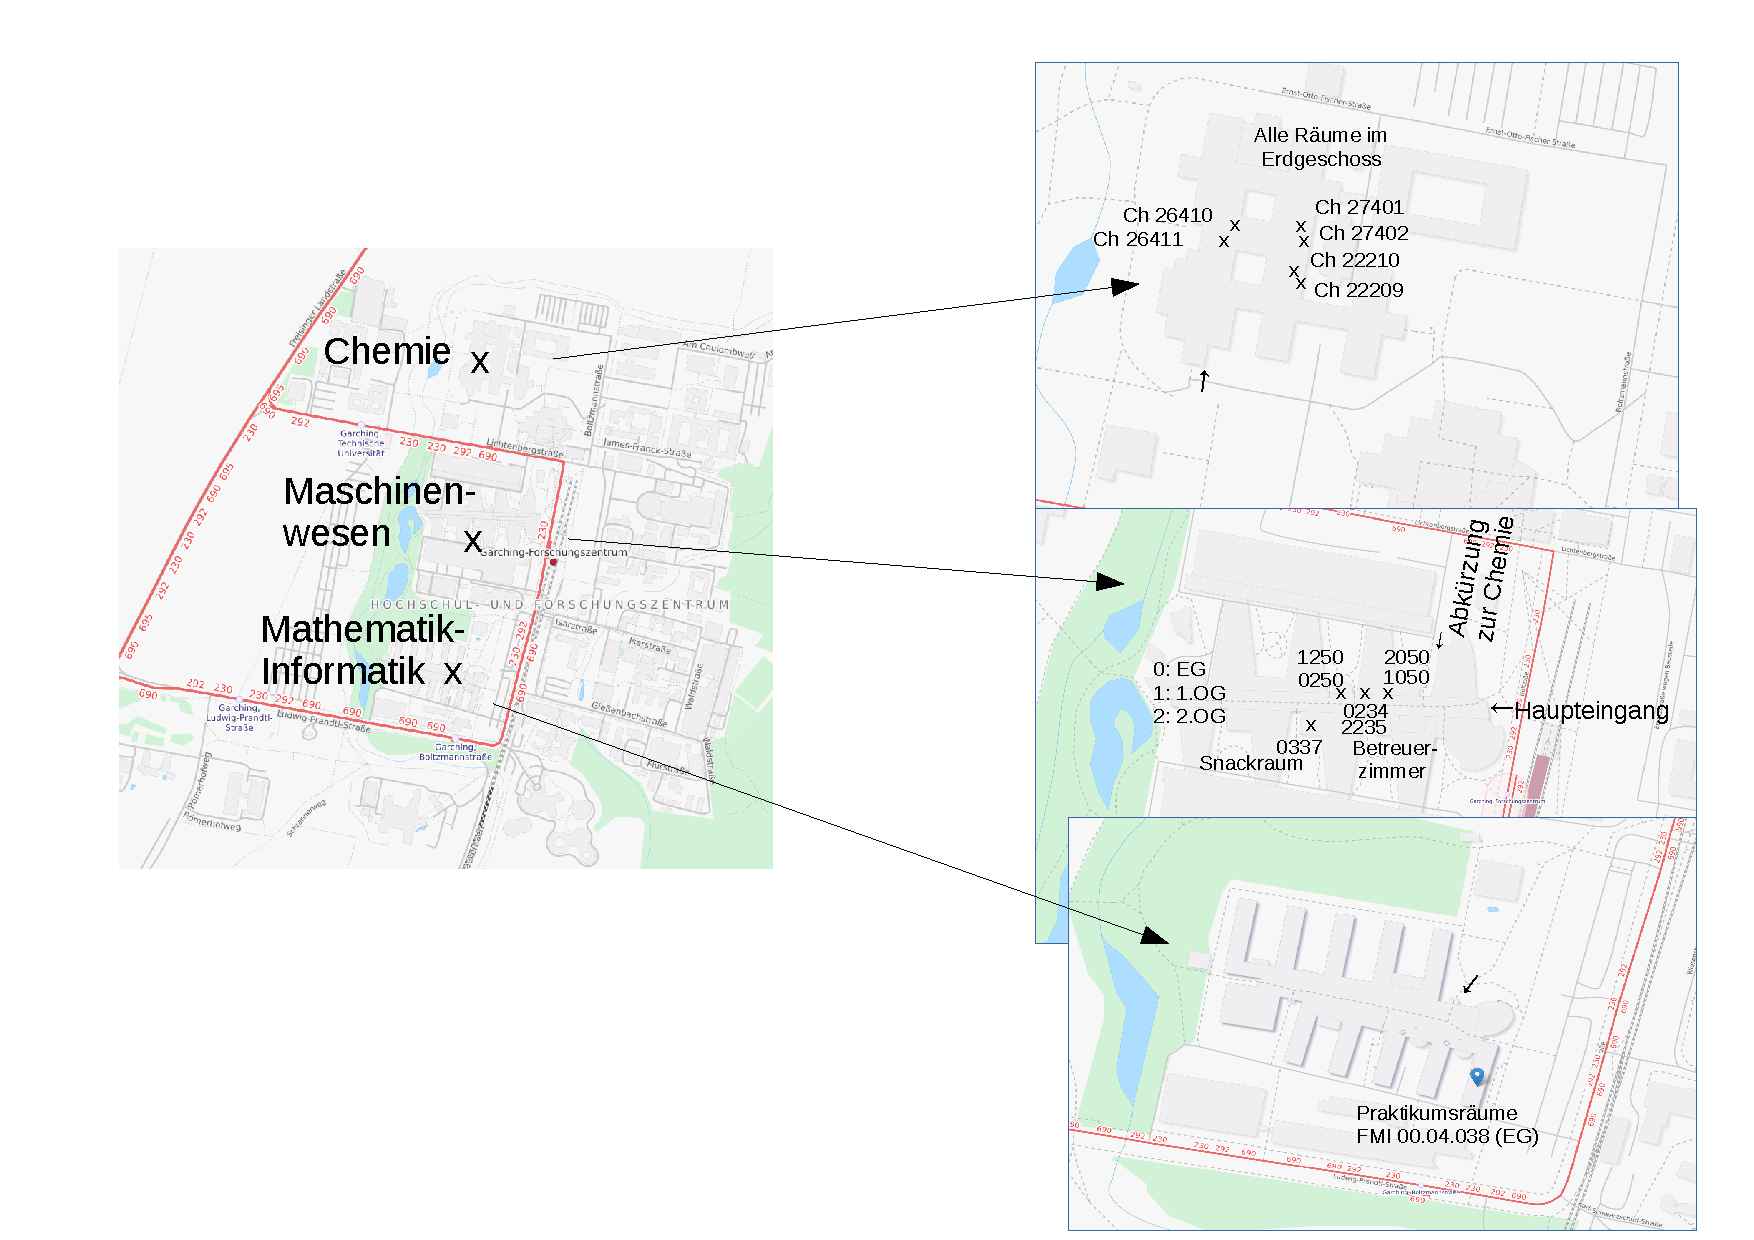
\includegraphics[scale=0.5]{campus_map.pdf}
\end{figure}
\newpage{}\begin{center}{\huge{}\textbf{Stundenplan von Markus Eberhardt}}\end{center}\textbf{{\large{}Donnerstag}}\nopagebreak \\\begin{tabular} {|p{3cm} p{6cm} p{6cm}| }\hline \textbf{11:30 bis 13:45}&\textbf{Anreise zur TU München}&\textbf{Fakultät Maschinenwesen}\\\hline \textbf{12:00 bis 13:30}&\textbf{Mittagessen}&\textbf{Mensa Garching}\\\hline \textbf{14:00}&\textbf{Begrüßung}&\textbf{CH 26411}\\&Begrüßung, Besprechung des Zeitplans, Ausgabe der individuellen Stundenpläne,...&\\\hline \textbf{14:50 bis 16:20}&\textbf{Quanten- und Atomphysik I}&\textbf{CH 26410}\\&Betreuer: Ismail Achmed-Zade&ca. 28 Teilnehmer\\\hline \textbf{16:40 bis 18:10}&\textbf{Himmelsmechanik}&\textbf{MW 2050}\\&Betreuer: Lars Dehlwes&ca. 19 Teilnehmer\\\hline \textbf{18:30}&\textbf{Fahrt zur Jugendherberge}&\textbf{}\\\hline \textbf{19:00}&\textbf{Abendessen}&\textbf{Jugendherberge}\\\hline \end{tabular}\\\vspace{5.00000mm}~\\\textbf{{\large{}Freitag}}\nopagebreak \\\begin{tabular} {|p{3cm} p{6cm} p{6cm}| }\hline \textbf{06:30 bis 09:00}&\textbf{Frühstück}&\textbf{Jugendherberge}\\\hline \textbf{09:00 bis 13:00}&frei&\\\hline \textbf{13:00 bis 14:00}&\textbf{Mittagessen}&\textbf{Mensa Garching}\\\hline \textbf{14:20 bis 15:50}&\textbf{Experiment Brückenschaltung}&\textbf{Praktikum Brückenschaltung}\\&Betreuer: Martin Großhauser&ca. 6 Teilnehmer\\\hline \textbf{16:10 bis 17:40}&\textbf{Komplexe Wechselstromrechnung}&\textbf{MW 1050}\\&Betreuer: Vincent Grande&ca. 8 Teilnehmer\\\hline \textbf{18:00 bis 18:20}&\textbf{Erlebnisbericht IPhO}&\textbf{CH 26411}\\\hline \textbf{18:30}&\textbf{Fahrt zur Jugendherberge}&\textbf{}\\\hline \textbf{19:00}&\textbf{Abendessen}&\textbf{Jugendherberge}\\\hline \end{tabular}\\\vspace{5.00000mm}~\\\textbf{{\large{}Samstag}}\nopagebreak \\\begin{tabular} {|p{3cm} p{6cm} p{6cm}| }\hline \textbf{06:30 bis 08:00}&\textbf{Frühstück}&\textbf{Jugendherberge}\\\hline \textbf{08:00}&\textbf{Fahrt zur TU}&\textbf{}\\\hline \textbf{09:00 bis 10:30}&\textbf{Elektrodynamik 1}&\textbf{MW 1250}\\&Betreuer: Maximilian Keitel&ca. 21 Teilnehmer\\\hline \textbf{10:50 bis 12:20}&\textbf{Elektrodynamik 2}&\textbf{MW 1250}\\&Betreuer: Maximilian Keitel&ca. 21 Teilnehmer\\\hline \textbf{12:40 bis 14:00}&\textbf{Mittagessen}&\textbf{Fakultät Maschinenwesen}\\\hline \textbf{14:20 bis 15:50}&\textbf{Relativistische Teilchenphysik}&\textbf{CH 22210}\\&Betreuer: Lars Dehlwes&ca. 23 Teilnehmer\\\hline \textbf{16:10 bis 17:40}&\textbf{Elektrische Blackboxen}&\textbf{Praktikum Blackboxen}\\&Betreuer: Eugen Dizer&ca. 6 Teilnehmer\\\hline \textbf{18:00 bis 18:20}&\textbf{Vorstellung GYPT}&\textbf{CH 26411}\\\hline \textbf{18:30}&\textbf{Fahrt zur Jugendherberge}&\textbf{}\\\hline \textbf{19:00}&\textbf{Abendessen}&\textbf{Jugendherberge}\\\hline \end{tabular}\\\vspace{5.00000mm}~\\\textbf{{\large{}Sonntag}}\nopagebreak \\\begin{tabular} {|p{3cm} p{6cm} p{6cm}| }\hline \textbf{06:30 bis 08:00}&\textbf{Frühstück}&\textbf{Jugendherberge}\\\hline \textbf{08:00}&\textbf{Fahrt zur TU}&\textbf{}\\\hline \textbf{09:00 bis 10:30}&\textbf{Gravitationsbeschleunigung}&\textbf{MW 1050}\\&Betreuer: Ann-Kathrin Raab&ca. 8 Teilnehmer\\\hline \textbf{10:50 bis 12:20}&\textbf{Bestimmung des Brechungskoeffizienten von Plexiglas}&\textbf{MW 0234}\\&Betreuer: Lilith Diringer&ca. 8 Teilnehmer\\\hline \textbf{12:40 bis 13:00}&\textbf{Verabschiedung}&\textbf{CH 26411}\\\hline \textbf{13:00}&\textbf{Individuelle Abreise}&\textbf{}\\\hline \textbf{13:00 bis 14:00}&\textbf{Mittagessen}&\textbf{}\\\hline \end{tabular}\\\vspace{5.00000mm}~\\
Notfallnummern: \\
Sven Jandura: xxxx xxxxxxxxx \\
Johannes Rothe: xxxx xxxxxxxxx \\

\large Hast du Lust, die Andern vom Seminar wiederzusehen?\\
\normalsize Dann komm doch einfach zum \textbf{Vereinstreffen}. Dazu musst du kein Vereinsmitglied sein. Neben interesannten Vorträgen und Exkursionen sind jede Menge Spiel und Spaß geplant. Schau in einem Monat einfach noch mal auf der Website vorbei. Wir freuen uns, wenn du dabei bist.

\begin{figure}[!h]
\includegraphics[scale=0.5]{campus_map.pdf}
\end{figure}
\newpage{}\begin{center}{\huge{}\textbf{Stundenplan von Markus Baier}}\end{center}\textbf{{\large{}Donnerstag}}\nopagebreak \\\begin{tabular} {|p{3cm} p{6cm} p{6cm}| }\hline \textbf{11:30 bis 13:45}&\textbf{Anreise zur TU München}&\textbf{Fakultät Maschinenwesen}\\\hline \textbf{12:00 bis 13:30}&\textbf{Mittagessen}&\textbf{Mensa Garching}\\\hline \textbf{14:00}&\textbf{Begrüßung}&\textbf{CH 26411}\\&Begrüßung, Besprechung des Zeitplans, Ausgabe der individuellen Stundenpläne,...&\\\hline \textbf{14:50 bis 16:20}&\textbf{Experimentieren und Auswerten}&\textbf{CH 26411}\\&Betreuer: Ann-Kathrin Raab&ca. 18 Teilnehmer\\\hline \textbf{16:40 bis 18:10}&\textbf{Näherungsmethoden}&\textbf{MW 0234}\\&Betreuer: Ilja Göthel&ca. 13 Teilnehmer\\\hline \textbf{18:30}&\textbf{Fahrt zur Jugendherberge}&\textbf{}\\\hline \textbf{19:00}&\textbf{Abendessen}&\textbf{Jugendherberge}\\\hline \end{tabular}\\\vspace{5.00000mm}~\\\textbf{{\large{}Freitag}}\nopagebreak \\\begin{tabular} {|p{3cm} p{6cm} p{6cm}| }\hline \textbf{06:30 bis 09:00}&\textbf{Frühstück}&\textbf{Jugendherberge}\\\hline \textbf{09:00 bis 13:00}&frei&\\\hline \textbf{13:00 bis 14:00}&\textbf{Mittagessen}&\textbf{Mensa Garching}\\\hline \textbf{14:20 bis 15:50}&\textbf{Rotationsbewegungen}&\textbf{MW 1050}\\&Betreuer: Vincent Grande&ca. 6 Teilnehmer\\\hline \textbf{16:10 bis 17:40}&\textbf{Einführung ins Integrieren}&\textbf{MW 2050}\\&Betreuer: Felix Wechsler&ca. 14 Teilnehmer\\\hline \textbf{18:00 bis 18:20}&\textbf{Erlebnisbericht IPhO}&\textbf{CH 26411}\\\hline \textbf{18:30}&\textbf{Fahrt zur Jugendherberge}&\textbf{}\\\hline \textbf{19:00}&\textbf{Abendessen}&\textbf{Jugendherberge}\\\hline \end{tabular}\\\vspace{5.00000mm}~\\\textbf{{\large{}Samstag}}\nopagebreak \\\begin{tabular} {|p{3cm} p{6cm} p{6cm}| }\hline \textbf{06:30 bis 08:00}&\textbf{Frühstück}&\textbf{Jugendherberge}\\\hline \textbf{08:00}&\textbf{Fahrt zur TU}&\textbf{}\\\hline \textbf{09:00 bis 10:30}&\textbf{Thermodynamik 2 - Statistische Physik}&\textbf{MW 1050}\\&Betreuer: Vitaly Andreev&ca. 17 Teilnehmer\\\hline \textbf{10:50 bis 12:20}&\textbf{Elektrodynamik 2}&\textbf{MW 1250}\\&Betreuer: Maximilian Keitel&ca. 21 Teilnehmer\\\hline \textbf{12:40 bis 14:00}&\textbf{Mittagessen}&\textbf{Fakultät Maschinenwesen}\\\hline \textbf{14:20 bis 15:50}&\textbf{Quanten- und Atomphysik I}&\textbf{CH 22209}\\&Betreuer: Vitaly Andreev&ca. 22 Teilnehmer\\\hline \textbf{16:10 bis 17:40}&\textbf{Wellenoptik}&\textbf{CH 26410}\\&Betreuer: Christopher Pfeiffer&ca. 7 Teilnehmer\\\hline \textbf{18:00 bis 18:20}&\textbf{Vorstellung GYPT}&\textbf{CH 26411}\\\hline \textbf{18:30}&\textbf{Fahrt zur Jugendherberge}&\textbf{}\\\hline \textbf{19:00}&\textbf{Abendessen}&\textbf{Jugendherberge}\\\hline \end{tabular}\\\vspace{5.00000mm}~\\\textbf{{\large{}Sonntag}}\nopagebreak \\\begin{tabular} {|p{3cm} p{6cm} p{6cm}| }\hline \textbf{06:30 bis 08:00}&\textbf{Frühstück}&\textbf{Jugendherberge}\\\hline \textbf{08:00}&\textbf{Fahrt zur TU}&\textbf{}\\\hline \textbf{09:00 bis 10:30}&\textbf{Quanten- und Atomphysik II}&\textbf{MW 1250}\\&Betreuer: Vitaly Andreev&ca. 15 Teilnehmer\\\hline \textbf{10:50 bis 12:20}&\textbf{Relativistische Teilchenphysik}&\textbf{CH 22210}\\&Betreuer: Lars Dehlwes&ca. 11 Teilnehmer\\\hline \textbf{12:40 bis 13:00}&\textbf{Verabschiedung}&\textbf{CH 26411}\\\hline \textbf{13:00}&\textbf{Individuelle Abreise}&\textbf{}\\\hline \textbf{13:00 bis 14:00}&\textbf{Mittagessen}&\textbf{}\\\hline \end{tabular}\\\vspace{5.00000mm}~\\
Notfallnummern: \\
Sven Jandura: xxxx xxxxxxxxx \\
Johannes Rothe: xxxx xxxxxxxxx \\

\large Hast du Lust, die Andern vom Seminar wiederzusehen?\\
\normalsize Dann komm doch einfach zum \textbf{Vereinstreffen}. Dazu musst du kein Vereinsmitglied sein. Neben interesannten Vorträgen und Exkursionen sind jede Menge Spiel und Spaß geplant. Schau in einem Monat einfach noch mal auf der Website vorbei. Wir freuen uns, wenn du dabei bist.

\begin{figure}[!h]
\includegraphics[scale=0.5]{campus_map.pdf}
\end{figure}
\newpage{}\begin{center}{\huge{}\textbf{Stundenplan von Marten Karl}}\end{center}\textbf{{\large{}Donnerstag}}\nopagebreak \\\begin{tabular} {|p{3cm} p{6cm} p{6cm}| }\hline \textbf{11:30 bis 13:45}&\textbf{Anreise zur TU München}&\textbf{Fakultät Maschinenwesen}\\\hline \textbf{12:00 bis 13:30}&\textbf{Mittagessen}&\textbf{Mensa Garching}\\\hline \textbf{14:00}&\textbf{Begrüßung}&\textbf{CH 26411}\\&Begrüßung, Besprechung des Zeitplans, Ausgabe der individuellen Stundenpläne,...&\\\hline \textbf{14:50 bis 16:20}&\textbf{Thermodynamik 1}&\textbf{MW 1250}\\&Betreuer: Maximilian Marienhagen&ca. 12 Teilnehmer\\\hline \textbf{16:40 bis 18:10}&\textbf{Einführung ins Integrieren}&\textbf{MW 1050}\\&Betreuer: Johannes Rothe&ca. 14 Teilnehmer\\\hline \textbf{18:30}&\textbf{Fahrt zur Jugendherberge}&\textbf{}\\\hline \textbf{19:00}&\textbf{Abendessen}&\textbf{Jugendherberge}\\\hline \end{tabular}\\\vspace{5.00000mm}~\\\textbf{{\large{}Freitag}}\nopagebreak \\\begin{tabular} {|p{3cm} p{6cm} p{6cm}| }\hline \textbf{06:30 bis 09:00}&\textbf{Frühstück}&\textbf{Jugendherberge}\\\hline \textbf{09:00 bis 13:00}&frei&\\\hline \textbf{13:00 bis 14:00}&\textbf{Mittagessen}&\textbf{Mensa Garching}\\\hline \textbf{14:20 bis 15:50}&\textbf{Gewöhnliche Differentialgleichungen}&\textbf{MW 1250}\\&Betreuer: Sven Jandura&ca. 20 Teilnehmer\\\hline \textbf{16:10 bis 17:40}&\textbf{Experiment Oszilloskop}&\textbf{Praktikum Oszilloskop}\\&Betreuer: Christopher Pfeiffer&ca. 6 Teilnehmer\\\hline \textbf{18:00 bis 18:20}&\textbf{Erlebnisbericht IPhO}&\textbf{CH 26411}\\\hline \textbf{18:30}&\textbf{Fahrt zur Jugendherberge}&\textbf{}\\\hline \textbf{19:00}&\textbf{Abendessen}&\textbf{Jugendherberge}\\\hline \end{tabular}\\\vspace{5.00000mm}~\\\textbf{{\large{}Samstag}}\nopagebreak \\\begin{tabular} {|p{3cm} p{6cm} p{6cm}| }\hline \textbf{06:30 bis 08:00}&\textbf{Frühstück}&\textbf{Jugendherberge}\\\hline \textbf{08:00}&\textbf{Fahrt zur TU}&\textbf{}\\\hline \textbf{09:00 bis 10:30}&\textbf{Experiment Millikan-Versuch}&\textbf{Praktikum Millikan-Versuch}\\&Betreuer: Samuel Moll&ca. 6 Teilnehmer\\\hline \textbf{10:50 bis 12:20}&\textbf{Quanten- und Atomphysik I}&\textbf{MW 2050}\\&Betreuer: Vitaly Andreev&ca. 13 Teilnehmer\\\hline \textbf{12:40 bis 14:00}&\textbf{Mittagessen}&\textbf{Fakultät Maschinenwesen}\\\hline \textbf{14:20 bis 15:50}&\textbf{Relativistische Teilchenphysik}&\textbf{CH 22210}\\&Betreuer: Lars Dehlwes&ca. 23 Teilnehmer\\\hline \textbf{16:10 bis 17:40}&\textbf{Quanten- und Atomphysik II}&\textbf{CH 22209}\\&Betreuer: Vitaly Andreev&ca. 28 Teilnehmer\\\hline \textbf{18:00 bis 18:20}&\textbf{Vorstellung GYPT}&\textbf{CH 26411}\\\hline \textbf{18:30}&\textbf{Fahrt zur Jugendherberge}&\textbf{}\\\hline \textbf{19:00}&\textbf{Abendessen}&\textbf{Jugendherberge}\\\hline \end{tabular}\\\vspace{5.00000mm}~\\\textbf{{\large{}Sonntag}}\nopagebreak \\\begin{tabular} {|p{3cm} p{6cm} p{6cm}| }\hline \textbf{06:30 bis 08:00}&\textbf{Frühstück}&\textbf{Jugendherberge}\\\hline \textbf{08:00}&\textbf{Fahrt zur TU}&\textbf{}\\\hline \textbf{09:00 bis 10:30}&\textbf{Gravitationsbeschleunigung}&\textbf{MW 1050}\\&Betreuer: Ann-Kathrin Raab&ca. 8 Teilnehmer\\\hline \textbf{10:50 bis 12:20}&\textbf{Aufgabenseminar Quanten- und Atomphysik und Struktur der Materie}&\textbf{MW 1250}\\&Betreuer: Vitaly Andreev&ca. 24 Teilnehmer\\\hline \textbf{12:40 bis 13:00}&\textbf{Verabschiedung}&\textbf{CH 26411}\\\hline \textbf{13:00}&\textbf{Individuelle Abreise}&\textbf{}\\\hline \textbf{13:00 bis 14:00}&\textbf{Mittagessen}&\textbf{}\\\hline \end{tabular}\\\vspace{5.00000mm}~\\
Notfallnummern: \\
Sven Jandura: xxxx xxxxxxxxx \\
Johannes Rothe: xxxx xxxxxxxxx \\

\large Hast du Lust, die Andern vom Seminar wiederzusehen?\\
\normalsize Dann komm doch einfach zum \textbf{Vereinstreffen}. Dazu musst du kein Vereinsmitglied sein. Neben interesannten Vorträgen und Exkursionen sind jede Menge Spiel und Spaß geplant. Schau in einem Monat einfach noch mal auf der Website vorbei. Wir freuen uns, wenn du dabei bist.

\begin{figure}[!h]
\includegraphics[scale=0.5]{campus_map.pdf}
\end{figure}
\newpage{}\begin{center}{\huge{}\textbf{Stundenplan von Max Schneider}}\end{center}\textbf{{\large{}Donnerstag}}\nopagebreak \\\begin{tabular} {|p{3cm} p{6cm} p{6cm}| }\hline \textbf{11:30 bis 13:45}&\textbf{Anreise zur TU München}&\textbf{Fakultät Maschinenwesen}\\\hline \textbf{12:00 bis 13:30}&\textbf{Mittagessen}&\textbf{Mensa Garching}\\\hline \textbf{14:00}&\textbf{Begrüßung}&\textbf{CH 26411}\\&Begrüßung, Besprechung des Zeitplans, Ausgabe der individuellen Stundenpläne,...&\\\hline \textbf{14:50 bis 16:20}&\textbf{Spezielle Funktionen und Vektorrechnung}&\textbf{MW 0234}\\&Betreuer: Lilith Diringer&ca. 4 Teilnehmer\\\hline \textbf{16:40 bis 18:10}&\textbf{Klassische Mechanik}&\textbf{MW 1250}\\&Betreuer: Maximilian Marienhagen&ca. 10 Teilnehmer\\\hline \textbf{18:30}&\textbf{Fahrt zur Jugendherberge}&\textbf{}\\\hline \textbf{19:00}&\textbf{Abendessen}&\textbf{Jugendherberge}\\\hline \end{tabular}\\\vspace{5.00000mm}~\\\textbf{{\large{}Freitag}}\nopagebreak \\\begin{tabular} {|p{3cm} p{6cm} p{6cm}| }\hline \textbf{06:30 bis 09:00}&\textbf{Frühstück}&\textbf{Jugendherberge}\\\hline \textbf{09:00 bis 13:00}&frei&\\\hline \textbf{13:00 bis 14:00}&\textbf{Mittagessen}&\textbf{Mensa Garching}\\\hline \textbf{14:20 bis 15:50}&\textbf{Gewöhnliche Differentialgleichungen}&\textbf{MW 1250}\\&Betreuer: Sven Jandura&ca. 20 Teilnehmer\\\hline \textbf{16:10 bis 17:40}&\textbf{Näherungsmethoden}&\textbf{CH 26410}\\&Betreuer: Vincent Grande&ca. 11 Teilnehmer\\\hline \textbf{18:00 bis 18:20}&\textbf{Erlebnisbericht IPhO}&\textbf{CH 26411}\\\hline \textbf{18:30}&\textbf{Fahrt zur Jugendherberge}&\textbf{}\\\hline \textbf{19:00}&\textbf{Abendessen}&\textbf{Jugendherberge}\\\hline \end{tabular}\\\vspace{5.00000mm}~\\\textbf{{\large{}Samstag}}\nopagebreak \\\begin{tabular} {|p{3cm} p{6cm} p{6cm}| }\hline \textbf{06:30 bis 08:00}&\textbf{Frühstück}&\textbf{Jugendherberge}\\\hline \textbf{08:00}&\textbf{Fahrt zur TU}&\textbf{}\\\hline \textbf{09:00 bis 10:30}&\textbf{Elektrodynamik 1}&\textbf{MW 1250}\\&Betreuer: Maximilian Keitel&ca. 21 Teilnehmer\\\hline \textbf{10:50 bis 12:20}&\textbf{Spezielle Relativitätstheorie}&\textbf{MW 0250}\\&Betreuer: Johannes Rothe&ca. 12 Teilnehmer\\\hline \textbf{12:40 bis 14:00}&\textbf{Mittagessen}&\textbf{Fakultät Maschinenwesen}\\\hline \textbf{14:20 bis 15:50}&\textbf{Quanten- und Atomphysik I}&\textbf{CH 22209}\\&Betreuer: Vitaly Andreev&ca. 22 Teilnehmer\\\hline \textbf{16:10 bis 17:40}&\textbf{Quanten- und Atomphysik II}&\textbf{CH 22209}\\&Betreuer: Vitaly Andreev&ca. 28 Teilnehmer\\\hline \textbf{18:00 bis 18:20}&\textbf{Vorstellung GYPT}&\textbf{CH 26411}\\\hline \textbf{18:30}&\textbf{Fahrt zur Jugendherberge}&\textbf{}\\\hline \textbf{19:00}&\textbf{Abendessen}&\textbf{Jugendherberge}\\\hline \end{tabular}\\\vspace{5.00000mm}~\\\textbf{{\large{}Sonntag}}\nopagebreak \\\begin{tabular} {|p{3cm} p{6cm} p{6cm}| }\hline \textbf{06:30 bis 08:00}&\textbf{Frühstück}&\textbf{Jugendherberge}\\\hline \textbf{08:00}&\textbf{Fahrt zur TU}&\textbf{}\\\hline \textbf{09:00 bis 10:30}&\textbf{Theoretische Mechanik}&\textbf{CH 22210}\\&Betreuer: Eugen Dizer&ca. 13 Teilnehmer\\\hline \textbf{10:50 bis 12:20}&\textbf{Rotationsbewegungen}&\textbf{CH 26410}\\&Betreuer: Vincent Grande&ca. 9 Teilnehmer\\\hline \textbf{12:40 bis 13:00}&\textbf{Verabschiedung}&\textbf{CH 26411}\\\hline \textbf{13:00}&\textbf{Individuelle Abreise}&\textbf{}\\\hline \textbf{13:00 bis 14:00}&\textbf{Mittagessen}&\textbf{}\\\hline \end{tabular}\\\vspace{5.00000mm}~\\
Notfallnummern: \\
Sven Jandura: xxxx xxxxxxxxx \\
Johannes Rothe: xxxx xxxxxxxxx \\

\large Hast du Lust, die Andern vom Seminar wiederzusehen?\\
\normalsize Dann komm doch einfach zum \textbf{Vereinstreffen}. Dazu musst du kein Vereinsmitglied sein. Neben interesannten Vorträgen und Exkursionen sind jede Menge Spiel und Spaß geplant. Schau in einem Monat einfach noch mal auf der Website vorbei. Wir freuen uns, wenn du dabei bist.

\begin{figure}[!h]
\includegraphics[scale=0.5]{campus_map.pdf}
\end{figure}
\newpage{}\begin{center}{\huge{}\textbf{Stundenplan von Max Reichert}}\end{center}\textbf{{\large{}Donnerstag}}\nopagebreak \\\begin{tabular} {|p{3cm} p{6cm} p{6cm}| }\hline \textbf{11:30 bis 13:45}&\textbf{Anreise zur TU München}&\textbf{Fakultät Maschinenwesen}\\\hline \textbf{12:00 bis 13:30}&\textbf{Mittagessen}&\textbf{Mensa Garching}\\\hline \textbf{14:00}&\textbf{Begrüßung}&\textbf{CH 26411}\\&Begrüßung, Besprechung des Zeitplans, Ausgabe der individuellen Stundenpläne,...&\\\hline \textbf{14:50 bis 16:20}&\textbf{Quanten- und Atomphysik I}&\textbf{CH 26410}\\&Betreuer: Ismail Achmed-Zade&ca. 28 Teilnehmer\\\hline \textbf{16:40 bis 18:10}&\textbf{Geometrische Optik}&\textbf{MW 0250}\\&Betreuer: Christopher Pfeiffer&ca. 13 Teilnehmer\\\hline \textbf{18:30}&\textbf{Fahrt zur Jugendherberge}&\textbf{}\\\hline \textbf{19:00}&\textbf{Abendessen}&\textbf{Jugendherberge}\\\hline \end{tabular}\\\vspace{5.00000mm}~\\\textbf{{\large{}Freitag}}\nopagebreak \\\begin{tabular} {|p{3cm} p{6cm} p{6cm}| }\hline \textbf{06:30 bis 09:00}&\textbf{Frühstück}&\textbf{Jugendherberge}\\\hline \textbf{09:00 bis 13:00}&\textbf{Besichtigung der Forschungsneutronenquelle FRM II}&\textbf{MW 2050}\\&Betreuer: Felix Wechsler&ca. 28 Teilnehmer\\\hline \textbf{13:00 bis 14:00}&\textbf{Mittagessen}&\textbf{Mensa Garching}\\\hline \textbf{14:20 bis 15:50}&\textbf{Gewöhnliche Differentialgleichungen}&\textbf{MW 1250}\\&Betreuer: Sven Jandura&ca. 20 Teilnehmer\\\hline \textbf{16:10 bis 17:40}&\textbf{Experimentieren und Auswerten}&\textbf{CH 26411}\\&Betreuer: Ann-Kathrin Raab&ca. 3 Teilnehmer\\\hline \textbf{18:00 bis 18:20}&\textbf{Erlebnisbericht IPhO}&\textbf{CH 26411}\\\hline \textbf{18:30}&\textbf{Fahrt zur Jugendherberge}&\textbf{}\\\hline \textbf{19:00}&\textbf{Abendessen}&\textbf{Jugendherberge}\\\hline \end{tabular}\\\vspace{5.00000mm}~\\\textbf{{\large{}Samstag}}\nopagebreak \\\begin{tabular} {|p{3cm} p{6cm} p{6cm}| }\hline \textbf{06:30 bis 08:00}&\textbf{Frühstück}&\textbf{Jugendherberge}\\\hline \textbf{08:00}&\textbf{Fahrt zur TU}&\textbf{}\\\hline \textbf{09:00 bis 10:30}&\textbf{Thermodynamik 2 - Statistische Physik}&\textbf{MW 1050}\\&Betreuer: Vitaly Andreev&ca. 17 Teilnehmer\\\hline \textbf{10:50 bis 12:20}&\textbf{Spezielle Relativitätstheorie}&\textbf{MW 0250}\\&Betreuer: Johannes Rothe&ca. 12 Teilnehmer\\\hline \textbf{12:40 bis 14:00}&\textbf{Mittagessen}&\textbf{Fakultät Maschinenwesen}\\\hline \textbf{14:20 bis 15:50}&\textbf{Harmonische Schwingungen}&\textbf{CH 26411}\\&Betreuer: Ilja Göthel&ca. 3 Teilnehmer\\\hline \textbf{16:10 bis 17:40}&\textbf{Wellenoptik}&\textbf{CH 26410}\\&Betreuer: Christopher Pfeiffer&ca. 7 Teilnehmer\\\hline \textbf{18:00 bis 18:20}&\textbf{Vorstellung GYPT}&\textbf{CH 26411}\\\hline \textbf{18:30}&\textbf{Fahrt zur Jugendherberge}&\textbf{}\\\hline \textbf{19:00}&\textbf{Abendessen}&\textbf{Jugendherberge}\\\hline \end{tabular}\\\vspace{5.00000mm}~\\\textbf{{\large{}Sonntag}}\nopagebreak \\\begin{tabular} {|p{3cm} p{6cm} p{6cm}| }\hline \textbf{06:30 bis 08:00}&\textbf{Frühstück}&\textbf{Jugendherberge}\\\hline \textbf{08:00}&\textbf{Fahrt zur TU}&\textbf{}\\\hline \textbf{09:00 bis 10:30}&\textbf{Theoretische Mechanik}&\textbf{CH 22210}\\&Betreuer: Eugen Dizer&ca. 13 Teilnehmer\\\hline \textbf{10:50 bis 12:20}&\textbf{Elektrodynamik 2}&\textbf{MW 2050}\\&Betreuer: Maximilian Keitel&ca. 5 Teilnehmer\\\hline \textbf{12:40 bis 13:00}&\textbf{Verabschiedung}&\textbf{CH 26411}\\\hline \textbf{13:00}&\textbf{Individuelle Abreise}&\textbf{}\\\hline \textbf{13:00 bis 14:00}&\textbf{Mittagessen}&\textbf{}\\\hline \end{tabular}\\\vspace{5.00000mm}~\\
Notfallnummern: \\
Sven Jandura: xxxx xxxxxxxxx \\
Johannes Rothe: xxxx xxxxxxxxx \\

\large Hast du Lust, die Andern vom Seminar wiederzusehen?\\
\normalsize Dann komm doch einfach zum \textbf{Vereinstreffen}. Dazu musst du kein Vereinsmitglied sein. Neben interesannten Vorträgen und Exkursionen sind jede Menge Spiel und Spaß geplant. Schau in einem Monat einfach noch mal auf der Website vorbei. Wir freuen uns, wenn du dabei bist.

\begin{figure}[!h]
\includegraphics[scale=0.5]{campus_map.pdf}
\end{figure}
\newpage{}\begin{center}{\huge{}\textbf{Stundenplan von Maximilian Hofschen}}\end{center}\textbf{{\large{}Donnerstag}}\nopagebreak \\\begin{tabular} {|p{3cm} p{6cm} p{6cm}| }\hline \textbf{11:30 bis 13:45}&\textbf{Anreise zur TU München}&\textbf{Fakultät Maschinenwesen}\\\hline \textbf{12:00 bis 13:30}&\textbf{Mittagessen}&\textbf{Mensa Garching}\\\hline \textbf{14:00}&\textbf{Begrüßung}&\textbf{CH 26411}\\&Begrüßung, Besprechung des Zeitplans, Ausgabe der individuellen Stundenpläne,...&\\\hline \textbf{14:50 bis 16:20}&\textbf{Elektrische Schaltungen}&\textbf{MW 0250}\\&Betreuer: Christopher Pfeiffer&ca. 16 Teilnehmer\\\hline \textbf{16:40 bis 18:10}&\textbf{Geometrische Optik}&\textbf{MW 0250}\\&Betreuer: Christopher Pfeiffer&ca. 13 Teilnehmer\\\hline \textbf{18:30}&\textbf{Fahrt zur Jugendherberge}&\textbf{}\\\hline \textbf{19:00}&\textbf{Abendessen}&\textbf{Jugendherberge}\\\hline \end{tabular}\\\vspace{5.00000mm}~\\\textbf{{\large{}Freitag}}\nopagebreak \\\begin{tabular} {|p{3cm} p{6cm} p{6cm}| }\hline \textbf{06:30 bis 09:00}&\textbf{Frühstück}&\textbf{Jugendherberge}\\\hline \textbf{09:00 bis 13:00}&frei&\\\hline \textbf{13:00 bis 14:00}&\textbf{Mittagessen}&\textbf{Mensa Garching}\\\hline \textbf{14:20 bis 15:50}&\textbf{Rotationsbewegungen}&\textbf{MW 1050}\\&Betreuer: Vincent Grande&ca. 6 Teilnehmer\\\hline \textbf{16:10 bis 17:40}&\textbf{Experiment Brückenschaltung}&\textbf{Praktikum Brückenschaltung}\\&Betreuer: Martin Großhauser&ca. 6 Teilnehmer\\\hline \textbf{18:00 bis 18:20}&\textbf{Erlebnisbericht IPhO}&\textbf{CH 26411}\\\hline \textbf{18:30}&\textbf{Fahrt zur Jugendherberge}&\textbf{}\\\hline \textbf{19:00}&\textbf{Abendessen}&\textbf{Jugendherberge}\\\hline \end{tabular}\\\vspace{5.00000mm}~\\\textbf{{\large{}Samstag}}\nopagebreak \\\begin{tabular} {|p{3cm} p{6cm} p{6cm}| }\hline \textbf{06:30 bis 08:00}&\textbf{Frühstück}&\textbf{Jugendherberge}\\\hline \textbf{08:00}&\textbf{Fahrt zur TU}&\textbf{}\\\hline \textbf{09:00 bis 10:30}&\textbf{Experimentieren und Auswerten}&\textbf{CH 26411}\\&Betreuer: Ann-Kathrin Raab&ca. 18 Teilnehmer\\\hline \textbf{10:50 bis 12:20}&\textbf{Elektrodynamik 2}&\textbf{MW 1250}\\&Betreuer: Maximilian Keitel&ca. 21 Teilnehmer\\\hline \textbf{12:40 bis 14:00}&\textbf{Mittagessen}&\textbf{Fakultät Maschinenwesen}\\\hline \textbf{14:20 bis 15:50}&\textbf{Harmonische Schwingungen}&\textbf{CH 26411}\\&Betreuer: Ilja Göthel&ca. 3 Teilnehmer\\\hline \textbf{16:10 bis 17:40}&\textbf{Komplexe Wechselstromrechnung}&\textbf{MW 0250}\\&Betreuer: Vincent Grande&ca. 13 Teilnehmer\\\hline \textbf{18:00 bis 18:20}&\textbf{Vorstellung GYPT}&\textbf{CH 26411}\\\hline \textbf{18:30}&\textbf{Fahrt zur Jugendherberge}&\textbf{}\\\hline \textbf{19:00}&\textbf{Abendessen}&\textbf{Jugendherberge}\\\hline \end{tabular}\\\vspace{5.00000mm}~\\\textbf{{\large{}Sonntag}}\nopagebreak \\\begin{tabular} {|p{3cm} p{6cm} p{6cm}| }\hline \textbf{06:30 bis 08:00}&\textbf{Frühstück}&\textbf{Jugendherberge}\\\hline \textbf{08:00}&\textbf{Fahrt zur TU}&\textbf{}\\\hline \textbf{09:00 bis 10:30}&\textbf{Elektronik}&\textbf{CH 26410}\\&Betreuer: Martin Großhauser&ca. 10 Teilnehmer\\\hline \textbf{10:50 bis 12:20}&\textbf{Bestimmung des Brechungskoeffizienten von Plexiglas}&\textbf{MW 0234}\\&Betreuer: Lilith Diringer&ca. 8 Teilnehmer\\\hline \textbf{12:40 bis 13:00}&\textbf{Verabschiedung}&\textbf{CH 26411}\\\hline \textbf{13:00}&\textbf{Individuelle Abreise}&\textbf{}\\\hline \textbf{13:00 bis 14:00}&\textbf{Mittagessen}&\textbf{}\\\hline \end{tabular}\\\vspace{5.00000mm}~\\
Notfallnummern: \\
Sven Jandura: xxxx xxxxxxxxx \\
Johannes Rothe: xxxx xxxxxxxxx \\

\large Hast du Lust, die Andern vom Seminar wiederzusehen?\\
\normalsize Dann komm doch einfach zum \textbf{Vereinstreffen}. Dazu musst du kein Vereinsmitglied sein. Neben interesannten Vorträgen und Exkursionen sind jede Menge Spiel und Spaß geplant. Schau in einem Monat einfach noch mal auf der Website vorbei. Wir freuen uns, wenn du dabei bist.

\begin{figure}[!h]
\includegraphics[scale=0.5]{campus_map.pdf}
\end{figure}
\newpage{}\begin{center}{\huge{}\textbf{Stundenplan von Maximilian Adam}}\end{center}\textbf{{\large{}Donnerstag}}\nopagebreak \\\begin{tabular} {|p{3cm} p{6cm} p{6cm}| }\hline \textbf{11:30 bis 13:45}&\textbf{Anreise zur TU München}&\textbf{Fakultät Maschinenwesen}\\\hline \textbf{12:00 bis 13:30}&\textbf{Mittagessen}&\textbf{Mensa Garching}\\\hline \textbf{14:00}&\textbf{Begrüßung}&\textbf{CH 26411}\\&Begrüßung, Besprechung des Zeitplans, Ausgabe der individuellen Stundenpläne,...&\\\hline \textbf{14:50 bis 16:20}&\textbf{Thermodynamik 1}&\textbf{MW 1250}\\&Betreuer: Maximilian Marienhagen&ca. 12 Teilnehmer\\\hline \textbf{16:40 bis 18:10}&\textbf{Himmelsmechanik}&\textbf{MW 2050}\\&Betreuer: Lars Dehlwes&ca. 19 Teilnehmer\\\hline \textbf{18:30}&\textbf{Fahrt zur Jugendherberge}&\textbf{}\\\hline \textbf{19:00}&\textbf{Abendessen}&\textbf{Jugendherberge}\\\hline \end{tabular}\\\vspace{5.00000mm}~\\\textbf{{\large{}Freitag}}\nopagebreak \\\begin{tabular} {|p{3cm} p{6cm} p{6cm}| }\hline \textbf{06:30 bis 09:00}&\textbf{Frühstück}&\textbf{Jugendherberge}\\\hline \textbf{09:00 bis 13:00}&\textbf{Besichtigung der Forschungsneutronenquelle FRM II}&\textbf{MW 2050}\\&Betreuer: Felix Wechsler&ca. 28 Teilnehmer\\\hline \textbf{13:00 bis 14:00}&\textbf{Mittagessen}&\textbf{Mensa Garching}\\\hline \textbf{14:20 bis 15:50}&\textbf{Kernphysik}&\textbf{MW 0250}\\&Betreuer: Johannes Rothe&ca. 18 Teilnehmer\\\hline \textbf{16:10 bis 17:40}&\textbf{Aufgabenseminar klassische Mechanik}&\textbf{CH 26410}\\&Betreuer: Aaron Wild&ca. 3 Teilnehmer\\\hline \textbf{18:00 bis 18:20}&\textbf{Erlebnisbericht IPhO}&\textbf{CH 26411}\\\hline \textbf{18:30}&\textbf{Fahrt zur Jugendherberge}&\textbf{}\\\hline \textbf{19:00}&\textbf{Abendessen}&\textbf{Jugendherberge}\\\hline \end{tabular}\\\vspace{5.00000mm}~\\\textbf{{\large{}Samstag}}\nopagebreak \\\begin{tabular} {|p{3cm} p{6cm} p{6cm}| }\hline \textbf{06:30 bis 08:00}&\textbf{Frühstück}&\textbf{Jugendherberge}\\\hline \textbf{08:00}&\textbf{Fahrt zur TU}&\textbf{}\\\hline \textbf{09:00 bis 10:30}&\textbf{Experimentieren und Auswerten}&\textbf{CH 26411}\\&Betreuer: Ann-Kathrin Raab&ca. 18 Teilnehmer\\\hline \textbf{10:50 bis 12:20}&\textbf{Quanten- und Atomphysik I}&\textbf{MW 2050}\\&Betreuer: Vitaly Andreev&ca. 13 Teilnehmer\\\hline \textbf{12:40 bis 14:00}&\textbf{Mittagessen}&\textbf{Fakultät Maschinenwesen}\\\hline \textbf{14:20 bis 15:50}&\textbf{Bestimmung des Brechungskoeffizienten von Plexiglas}&\textbf{MW 0234}\\&Betreuer: Lilith Diringer&ca. 8 Teilnehmer\\\hline \textbf{16:10 bis 17:40}&\textbf{Quanten- und Atomphysik II}&\textbf{CH 22209}\\&Betreuer: Vitaly Andreev&ca. 28 Teilnehmer\\\hline \textbf{18:00 bis 18:20}&\textbf{Vorstellung GYPT}&\textbf{CH 26411}\\\hline \textbf{18:30}&\textbf{Fahrt zur Jugendherberge}&\textbf{}\\\hline \textbf{19:00}&\textbf{Abendessen}&\textbf{Jugendherberge}\\\hline \end{tabular}\\\vspace{5.00000mm}~\\\textbf{{\large{}Sonntag}}\nopagebreak \\\begin{tabular} {|p{3cm} p{6cm} p{6cm}| }\hline \textbf{06:30 bis 08:00}&\textbf{Frühstück}&\textbf{Jugendherberge}\\\hline \textbf{08:00}&\textbf{Fahrt zur TU}&\textbf{}\\\hline \textbf{09:00 bis 10:30}&\textbf{Elektronik}&\textbf{CH 26410}\\&Betreuer: Martin Großhauser&ca. 10 Teilnehmer\\\hline \textbf{10:50 bis 12:20}&\textbf{Aufgabenseminar Quanten- und Atomphysik und Struktur der Materie}&\textbf{MW 1250}\\&Betreuer: Vitaly Andreev&ca. 24 Teilnehmer\\\hline \textbf{12:40 bis 13:00}&\textbf{Verabschiedung}&\textbf{CH 26411}\\\hline \textbf{13:00}&\textbf{Individuelle Abreise}&\textbf{}\\\hline \textbf{13:00 bis 14:00}&\textbf{Mittagessen}&\textbf{}\\\hline \end{tabular}\\\vspace{5.00000mm}~\\
Notfallnummern: \\
Sven Jandura: xxxx xxxxxxxxx \\
Johannes Rothe: xxxx xxxxxxxxx \\

\large Hast du Lust, die Andern vom Seminar wiederzusehen?\\
\normalsize Dann komm doch einfach zum \textbf{Vereinstreffen}. Dazu musst du kein Vereinsmitglied sein. Neben interesannten Vorträgen und Exkursionen sind jede Menge Spiel und Spaß geplant. Schau in einem Monat einfach noch mal auf der Website vorbei. Wir freuen uns, wenn du dabei bist.

\begin{figure}[!h]
\includegraphics[scale=0.5]{campus_map.pdf}
\end{figure}
\newpage{}\begin{center}{\huge{}\textbf{Stundenplan von Maximilian Herzog}}\end{center}\textbf{{\large{}Donnerstag}}\nopagebreak \\\begin{tabular} {|p{3cm} p{6cm} p{6cm}| }\hline \textbf{11:30 bis 13:45}&\textbf{Anreise zur TU München}&\textbf{Fakultät Maschinenwesen}\\\hline \textbf{12:00 bis 13:30}&\textbf{Mittagessen}&\textbf{Mensa Garching}\\\hline \textbf{14:00}&\textbf{Begrüßung}&\textbf{CH 26411}\\&Begrüßung, Besprechung des Zeitplans, Ausgabe der individuellen Stundenpläne,...&\\\hline \textbf{14:50 bis 16:20}&\textbf{Elektrische Schaltungen}&\textbf{MW 0250}\\&Betreuer: Christopher Pfeiffer&ca. 16 Teilnehmer\\\hline \textbf{16:40 bis 18:10}&\textbf{Himmelsmechanik}&\textbf{MW 2050}\\&Betreuer: Lars Dehlwes&ca. 19 Teilnehmer\\\hline \textbf{18:30}&\textbf{Fahrt zur Jugendherberge}&\textbf{}\\\hline \textbf{19:00}&\textbf{Abendessen}&\textbf{Jugendherberge}\\\hline \end{tabular}\\\vspace{5.00000mm}~\\\textbf{{\large{}Freitag}}\nopagebreak \\\begin{tabular} {|p{3cm} p{6cm} p{6cm}| }\hline \textbf{06:30 bis 09:00}&\textbf{Frühstück}&\textbf{Jugendherberge}\\\hline \textbf{09:00 bis 13:00}&frei&\\\hline \textbf{13:00 bis 14:00}&\textbf{Mittagessen}&\textbf{Mensa Garching}\\\hline \textbf{14:20 bis 15:50}&\textbf{Kernphysik}&\textbf{MW 0250}\\&Betreuer: Johannes Rothe&ca. 18 Teilnehmer\\\hline \textbf{16:10 bis 17:40}&\textbf{Näherungsmethoden}&\textbf{CH 26410}\\&Betreuer: Vincent Grande&ca. 11 Teilnehmer\\\hline \textbf{18:00 bis 18:20}&\textbf{Erlebnisbericht IPhO}&\textbf{CH 26411}\\\hline \textbf{18:30}&\textbf{Fahrt zur Jugendherberge}&\textbf{}\\\hline \textbf{19:00}&\textbf{Abendessen}&\textbf{Jugendherberge}\\\hline \end{tabular}\\\vspace{5.00000mm}~\\\textbf{{\large{}Samstag}}\nopagebreak \\\begin{tabular} {|p{3cm} p{6cm} p{6cm}| }\hline \textbf{06:30 bis 08:00}&\textbf{Frühstück}&\textbf{Jugendherberge}\\\hline \textbf{08:00}&\textbf{Fahrt zur TU}&\textbf{}\\\hline \textbf{09:00 bis 10:30}&\textbf{Harmonische Schwingungen}&\textbf{MW 0250}\\&Betreuer: Ilja Göthel&ca. 9 Teilnehmer\\\hline \textbf{10:50 bis 12:20}&\textbf{Quanten- und Atomphysik I}&\textbf{MW 2050}\\&Betreuer: Vitaly Andreev&ca. 13 Teilnehmer\\\hline \textbf{12:40 bis 14:00}&\textbf{Mittagessen}&\textbf{Fakultät Maschinenwesen}\\\hline \textbf{14:20 bis 15:50}&\textbf{Bestimmung des Brechungskoeffizienten von Plexiglas}&\textbf{MW 0234}\\&Betreuer: Lilith Diringer&ca. 8 Teilnehmer\\\hline \textbf{16:10 bis 17:40}&\textbf{Bestimmung des Brechungskoeffizienten von Wasser}&\textbf{MW 0234}\\&Betreuer: Lilith Diringer&ca. 8 Teilnehmer\\\hline \textbf{18:00 bis 18:20}&\textbf{Vorstellung GYPT}&\textbf{CH 26411}\\\hline \textbf{18:30}&\textbf{Fahrt zur Jugendherberge}&\textbf{}\\\hline \textbf{19:00}&\textbf{Abendessen}&\textbf{Jugendherberge}\\\hline \end{tabular}\\\vspace{5.00000mm}~\\\textbf{{\large{}Sonntag}}\nopagebreak \\\begin{tabular} {|p{3cm} p{6cm} p{6cm}| }\hline \textbf{06:30 bis 08:00}&\textbf{Frühstück}&\textbf{Jugendherberge}\\\hline \textbf{08:00}&\textbf{Fahrt zur TU}&\textbf{}\\\hline \textbf{09:00 bis 10:30}&\textbf{Gravitationsbeschleunigung}&\textbf{MW 1050}\\&Betreuer: Ann-Kathrin Raab&ca. 8 Teilnehmer\\\hline \textbf{10:50 bis 12:20}&\textbf{Elektrische Blackboxen}&\textbf{Praktikum Blackboxen}\\&Betreuer: Eugen Dizer&ca. 6 Teilnehmer\\\hline \textbf{12:40 bis 13:00}&\textbf{Verabschiedung}&\textbf{CH 26411}\\\hline \textbf{13:00}&\textbf{Individuelle Abreise}&\textbf{}\\\hline \textbf{13:00 bis 14:00}&\textbf{Mittagessen}&\textbf{}\\\hline \end{tabular}\\\vspace{5.00000mm}~\\
Notfallnummern: \\
Sven Jandura: xxxx xxxxxxxxx \\
Johannes Rothe: xxxx xxxxxxxxx \\

\large Hast du Lust, die Andern vom Seminar wiederzusehen?\\
\normalsize Dann komm doch einfach zum \textbf{Vereinstreffen}. Dazu musst du kein Vereinsmitglied sein. Neben interesannten Vorträgen und Exkursionen sind jede Menge Spiel und Spaß geplant. Schau in einem Monat einfach noch mal auf der Website vorbei. Wir freuen uns, wenn du dabei bist.

\begin{figure}[!h]
\includegraphics[scale=0.5]{campus_map.pdf}
\end{figure}
\newpage{}\begin{center}{\huge{}\textbf{Stundenplan von Mia Sittinger}}\end{center}\textbf{{\large{}Donnerstag}}\nopagebreak \\\begin{tabular} {|p{3cm} p{6cm} p{6cm}| }\hline \textbf{11:30 bis 13:45}&\textbf{Anreise zur TU München}&\textbf{Fakultät Maschinenwesen}\\\hline \textbf{12:00 bis 13:30}&\textbf{Mittagessen}&\textbf{Mensa Garching}\\\hline \textbf{14:00}&\textbf{Begrüßung}&\textbf{CH 26411}\\&Begrüßung, Besprechung des Zeitplans, Ausgabe der individuellen Stundenpläne,...&\\\hline \textbf{14:50 bis 16:20}&\textbf{Experimentieren und Auswerten}&\textbf{CH 26411}\\&Betreuer: Ann-Kathrin Raab&ca. 18 Teilnehmer\\\hline \textbf{16:40 bis 18:10}&\textbf{Himmelsmechanik}&\textbf{MW 2050}\\&Betreuer: Lars Dehlwes&ca. 19 Teilnehmer\\\hline \textbf{18:30}&\textbf{Fahrt zur Jugendherberge}&\textbf{}\\\hline \textbf{19:00}&\textbf{Abendessen}&\textbf{Jugendherberge}\\\hline \end{tabular}\\\vspace{5.00000mm}~\\\textbf{{\large{}Freitag}}\nopagebreak \\\begin{tabular} {|p{3cm} p{6cm} p{6cm}| }\hline \textbf{06:30 bis 09:00}&\textbf{Frühstück}&\textbf{Jugendherberge}\\\hline \textbf{09:00 bis 13:00}&\textbf{Besichtigung der Forschungsneutronenquelle FRM II}&\textbf{MW 2050}\\&Betreuer: Felix Wechsler&ca. 28 Teilnehmer\\\hline \textbf{13:00 bis 14:00}&\textbf{Mittagessen}&\textbf{Mensa Garching}\\\hline \textbf{14:20 bis 15:50}&\textbf{Experiment spezifische Elektronenladung}&\textbf{Praktikum spezifische Elektronenladung}\\&Betreuer: Felix Wechsler&ca. 6 Teilnehmer\\\hline \textbf{16:10 bis 17:40}&\textbf{Einführung ins Integrieren}&\textbf{MW 2050}\\&Betreuer: Felix Wechsler&ca. 14 Teilnehmer\\\hline \textbf{18:00 bis 18:20}&\textbf{Erlebnisbericht IPhO}&\textbf{CH 26411}\\\hline \textbf{18:30}&\textbf{Fahrt zur Jugendherberge}&\textbf{}\\\hline \textbf{19:00}&\textbf{Abendessen}&\textbf{Jugendherberge}\\\hline \end{tabular}\\\vspace{5.00000mm}~\\\textbf{{\large{}Samstag}}\nopagebreak \\\begin{tabular} {|p{3cm} p{6cm} p{6cm}| }\hline \textbf{06:30 bis 08:00}&\textbf{Frühstück}&\textbf{Jugendherberge}\\\hline \textbf{08:00}&\textbf{Fahrt zur TU}&\textbf{}\\\hline \textbf{09:00 bis 10:30}&\textbf{Thermodynamik 2 - Statistische Physik}&\textbf{MW 1050}\\&Betreuer: Vitaly Andreev&ca. 17 Teilnehmer\\\hline \textbf{10:50 bis 12:20}&\textbf{Elektrodynamik 2}&\textbf{MW 1250}\\&Betreuer: Maximilian Keitel&ca. 21 Teilnehmer\\\hline \textbf{12:40 bis 14:00}&\textbf{Mittagessen}&\textbf{Fakultät Maschinenwesen}\\\hline \textbf{14:20 bis 15:50}&\textbf{Gravitationsbeschleunigung}&\textbf{MW 1050}\\&Betreuer: Ann-Kathrin Raab&ca. 8 Teilnehmer\\\hline \textbf{16:10 bis 17:40}&\textbf{Quanten- und Atomphysik II}&\textbf{CH 22209}\\&Betreuer: Vitaly Andreev&ca. 28 Teilnehmer\\\hline \textbf{18:00 bis 18:20}&\textbf{Vorstellung GYPT}&\textbf{CH 26411}\\\hline \textbf{18:30}&\textbf{Fahrt zur Jugendherberge}&\textbf{}\\\hline \textbf{19:00}&\textbf{Abendessen}&\textbf{Jugendherberge}\\\hline \end{tabular}\\\vspace{5.00000mm}~\\\textbf{{\large{}Sonntag}}\nopagebreak \\\begin{tabular} {|p{3cm} p{6cm} p{6cm}| }\hline \textbf{06:30 bis 08:00}&\textbf{Frühstück}&\textbf{Jugendherberge}\\\hline \textbf{08:00}&\textbf{Fahrt zur TU}&\textbf{}\\\hline \textbf{09:00 bis 10:30}&\textbf{Theoretische Mechanik}&\textbf{CH 22210}\\&Betreuer: Eugen Dizer&ca. 13 Teilnehmer\\\hline \textbf{10:50 bis 12:20}&\textbf{Relativistische Teilchenphysik}&\textbf{CH 22210}\\&Betreuer: Lars Dehlwes&ca. 11 Teilnehmer\\\hline \textbf{12:40 bis 13:00}&\textbf{Verabschiedung}&\textbf{CH 26411}\\\hline \textbf{13:00}&\textbf{Individuelle Abreise}&\textbf{}\\\hline \textbf{13:00 bis 14:00}&\textbf{Mittagessen}&\textbf{}\\\hline \end{tabular}\\\vspace{5.00000mm}~\\
Notfallnummern: \\
Sven Jandura: xxxx xxxxxxxxx \\
Johannes Rothe: xxxx xxxxxxxxx \\

\large Hast du Lust, die Andern vom Seminar wiederzusehen?\\
\normalsize Dann komm doch einfach zum \textbf{Vereinstreffen}. Dazu musst du kein Vereinsmitglied sein. Neben interesannten Vorträgen und Exkursionen sind jede Menge Spiel und Spaß geplant. Schau in einem Monat einfach noch mal auf der Website vorbei. Wir freuen uns, wenn du dabei bist.

\begin{figure}[!h]
\includegraphics[scale=0.5]{campus_map.pdf}
\end{figure}
\newpage{}\begin{center}{\huge{}\textbf{Stundenplan von Mia Begovic}}\end{center}\textbf{{\large{}Donnerstag}}\nopagebreak \\\begin{tabular} {|p{3cm} p{6cm} p{6cm}| }\hline \textbf{11:30 bis 13:45}&\textbf{Anreise zur TU München}&\textbf{Fakultät Maschinenwesen}\\\hline \textbf{12:00 bis 13:30}&\textbf{Mittagessen}&\textbf{Mensa Garching}\\\hline \textbf{14:00}&\textbf{Begrüßung}&\textbf{CH 26411}\\&Begrüßung, Besprechung des Zeitplans, Ausgabe der individuellen Stundenpläne,...&\\\hline \textbf{14:50 bis 16:20}&\textbf{Quanten- und Atomphysik I}&\textbf{CH 26410}\\&Betreuer: Ismail Achmed-Zade&ca. 28 Teilnehmer\\\hline \textbf{16:40 bis 18:10}&\textbf{Himmelsmechanik}&\textbf{MW 2050}\\&Betreuer: Lars Dehlwes&ca. 19 Teilnehmer\\\hline \textbf{18:30}&\textbf{Fahrt zur Jugendherberge}&\textbf{}\\\hline \textbf{19:00}&\textbf{Abendessen}&\textbf{Jugendherberge}\\\hline \end{tabular}\\\vspace{5.00000mm}~\\\textbf{{\large{}Freitag}}\nopagebreak \\\begin{tabular} {|p{3cm} p{6cm} p{6cm}| }\hline \textbf{06:30 bis 09:00}&\textbf{Frühstück}&\textbf{Jugendherberge}\\\hline \textbf{09:00 bis 13:00}&frei&\\\hline \textbf{13:00 bis 14:00}&\textbf{Mittagessen}&\textbf{Mensa Garching}\\\hline \textbf{14:20 bis 15:50}&\textbf{Einführung ins Differenzieren}&\textbf{CH 26411}\\&Betreuer: Ann-Kathrin Raab&ca. 5 Teilnehmer\\\hline \textbf{16:10 bis 17:40}&\textbf{Einführung ins Integrieren}&\textbf{MW 2050}\\&Betreuer: Felix Wechsler&ca. 14 Teilnehmer\\\hline \textbf{18:00 bis 18:20}&\textbf{Erlebnisbericht IPhO}&\textbf{CH 26411}\\\hline \textbf{18:30}&\textbf{Fahrt zur Jugendherberge}&\textbf{}\\\hline \textbf{19:00}&\textbf{Abendessen}&\textbf{Jugendherberge}\\\hline \end{tabular}\\\vspace{5.00000mm}~\\\textbf{{\large{}Samstag}}\nopagebreak \\\begin{tabular} {|p{3cm} p{6cm} p{6cm}| }\hline \textbf{06:30 bis 08:00}&\textbf{Frühstück}&\textbf{Jugendherberge}\\\hline \textbf{08:00}&\textbf{Fahrt zur TU}&\textbf{}\\\hline \textbf{09:00 bis 10:30}&\textbf{Experimentieren und Auswerten}&\textbf{CH 26411}\\&Betreuer: Ann-Kathrin Raab&ca. 18 Teilnehmer\\\hline \textbf{10:50 bis 12:20}&\textbf{Elektrodynamik 2}&\textbf{MW 1250}\\&Betreuer: Maximilian Keitel&ca. 21 Teilnehmer\\\hline \textbf{12:40 bis 14:00}&\textbf{Mittagessen}&\textbf{Fakultät Maschinenwesen}\\\hline \textbf{14:20 bis 15:50}&\textbf{Relativistische Teilchenphysik}&\textbf{CH 22210}\\&Betreuer: Lars Dehlwes&ca. 23 Teilnehmer\\\hline \textbf{16:10 bis 17:40}&\textbf{Quanten- und Atomphysik II}&\textbf{CH 22209}\\&Betreuer: Vitaly Andreev&ca. 28 Teilnehmer\\\hline \textbf{18:00 bis 18:20}&\textbf{Vorstellung GYPT}&\textbf{CH 26411}\\\hline \textbf{18:30}&\textbf{Fahrt zur Jugendherberge}&\textbf{}\\\hline \textbf{19:00}&\textbf{Abendessen}&\textbf{Jugendherberge}\\\hline \end{tabular}\\\vspace{5.00000mm}~\\\textbf{{\large{}Sonntag}}\nopagebreak \\\begin{tabular} {|p{3cm} p{6cm} p{6cm}| }\hline \textbf{06:30 bis 08:00}&\textbf{Frühstück}&\textbf{Jugendherberge}\\\hline \textbf{08:00}&\textbf{Fahrt zur TU}&\textbf{}\\\hline \textbf{09:00 bis 10:30}&\textbf{Spezielle Relativitätstheorie}&\textbf{MW 0250}\\&Betreuer: Johannes Rothe&ca. 12 Teilnehmer\\\hline \textbf{10:50 bis 12:20}&\textbf{Wellenoptik}&\textbf{MW 0250}\\&Betreuer: Christopher Pfeiffer&ca. 12 Teilnehmer\\\hline \textbf{12:40 bis 13:00}&\textbf{Verabschiedung}&\textbf{CH 26411}\\\hline \textbf{13:00}&\textbf{Individuelle Abreise}&\textbf{}\\\hline \textbf{13:00 bis 14:00}&\textbf{Mittagessen}&\textbf{}\\\hline \end{tabular}\\\vspace{5.00000mm}~\\
Notfallnummern: \\
Sven Jandura: xxxx xxxxxxxxx \\
Johannes Rothe: xxxx xxxxxxxxx \\

\large Hast du Lust, die Andern vom Seminar wiederzusehen?\\
\normalsize Dann komm doch einfach zum \textbf{Vereinstreffen}. Dazu musst du kein Vereinsmitglied sein. Neben interesannten Vorträgen und Exkursionen sind jede Menge Spiel und Spaß geplant. Schau in einem Monat einfach noch mal auf der Website vorbei. Wir freuen uns, wenn du dabei bist.

\begin{figure}[!h]
\includegraphics[scale=0.5]{campus_map.pdf}
\end{figure}
\newpage{}\begin{center}{\huge{}\textbf{Stundenplan von Natalie Adam}}\end{center}\textbf{{\large{}Donnerstag}}\nopagebreak \\\begin{tabular} {|p{3cm} p{6cm} p{6cm}| }\hline \textbf{11:30 bis 13:45}&\textbf{Anreise zur TU München}&\textbf{Fakultät Maschinenwesen}\\\hline \textbf{12:00 bis 13:30}&\textbf{Mittagessen}&\textbf{Mensa Garching}\\\hline \textbf{14:00}&\textbf{Begrüßung}&\textbf{CH 26411}\\&Begrüßung, Besprechung des Zeitplans, Ausgabe der individuellen Stundenpläne,...&\\\hline \textbf{14:50 bis 16:20}&\textbf{Elektrische Schaltungen}&\textbf{MW 0250}\\&Betreuer: Christopher Pfeiffer&ca. 16 Teilnehmer\\\hline \textbf{16:40 bis 18:10}&\textbf{Experimentieren und Auswerten}&\textbf{CH 26411}\\&Betreuer: Ann-Kathrin Raab&ca. 15 Teilnehmer\\\hline \textbf{18:30}&\textbf{Fahrt zur Jugendherberge}&\textbf{}\\\hline \textbf{19:00}&\textbf{Abendessen}&\textbf{Jugendherberge}\\\hline \end{tabular}\\\vspace{5.00000mm}~\\\textbf{{\large{}Freitag}}\nopagebreak \\\begin{tabular} {|p{3cm} p{6cm} p{6cm}| }\hline \textbf{06:30 bis 09:00}&\textbf{Frühstück}&\textbf{Jugendherberge}\\\hline \textbf{09:00 bis 13:00}&\textbf{Besichtigung der Forschungsneutronenquelle FRM II}&\textbf{MW 2050}\\&Betreuer: Felix Wechsler&ca. 28 Teilnehmer\\\hline \textbf{13:00 bis 14:00}&\textbf{Mittagessen}&\textbf{Mensa Garching}\\\hline \textbf{14:20 bis 15:50}&\textbf{Aufgabenseminar Wärmelehre}&\textbf{MW 2050}\\&Betreuer: Maximilian Marienhagen&ca. 9 Teilnehmer\\\hline \textbf{16:10 bis 17:40}&\textbf{Experiment Brückenschaltung}&\textbf{Praktikum Brückenschaltung}\\&Betreuer: Martin Großhauser&ca. 6 Teilnehmer\\\hline \textbf{18:00 bis 18:20}&\textbf{Erlebnisbericht IPhO}&\textbf{CH 26411}\\\hline \textbf{18:30}&\textbf{Fahrt zur Jugendherberge}&\textbf{}\\\hline \textbf{19:00}&\textbf{Abendessen}&\textbf{Jugendherberge}\\\hline \end{tabular}\\\vspace{5.00000mm}~\\\textbf{{\large{}Samstag}}\nopagebreak \\\begin{tabular} {|p{3cm} p{6cm} p{6cm}| }\hline \textbf{06:30 bis 08:00}&\textbf{Frühstück}&\textbf{Jugendherberge}\\\hline \textbf{08:00}&\textbf{Fahrt zur TU}&\textbf{}\\\hline \textbf{09:00 bis 10:30}&\textbf{Experiment Brennstoffzelle}&\textbf{Praktikum Brennstoffzelle}\\&Betreuer: Aaron Wild&ca. 6 Teilnehmer\\\hline \textbf{10:50 bis 12:20}&\textbf{Experiment Reversionspendel}&\textbf{Praktikum Reversionspendel}\\&Betreuer: Lilith Diringer&ca. 6 Teilnehmer\\\hline \textbf{12:40 bis 14:00}&\textbf{Mittagessen}&\textbf{Fakultät Maschinenwesen}\\\hline \textbf{14:20 bis 15:50}&\textbf{Gravitationsbeschleunigung}&\textbf{MW 1050}\\&Betreuer: Ann-Kathrin Raab&ca. 8 Teilnehmer\\\hline \textbf{16:10 bis 17:40}&\textbf{Elektrische Blackboxen}&\textbf{Praktikum Blackboxen}\\&Betreuer: Eugen Dizer&ca. 6 Teilnehmer\\\hline \textbf{18:00 bis 18:20}&\textbf{Vorstellung GYPT}&\textbf{CH 26411}\\\hline \textbf{18:30}&\textbf{Fahrt zur Jugendherberge}&\textbf{}\\\hline \textbf{19:00}&\textbf{Abendessen}&\textbf{Jugendherberge}\\\hline \end{tabular}\\\vspace{5.00000mm}~\\\textbf{{\large{}Sonntag}}\nopagebreak \\\begin{tabular} {|p{3cm} p{6cm} p{6cm}| }\hline \textbf{06:30 bis 08:00}&\textbf{Frühstück}&\textbf{Jugendherberge}\\\hline \textbf{08:00}&\textbf{Fahrt zur TU}&\textbf{}\\\hline \textbf{09:00 bis 10:30}&\textbf{Wellenoptik}&\textbf{MW 2050}\\&Betreuer: Christopher Pfeiffer&ca. 14 Teilnehmer\\\hline \textbf{10:50 bis 12:20}&\textbf{Bestimmung des Brechungskoeffizienten von Plexiglas}&\textbf{MW 0234}\\&Betreuer: Lilith Diringer&ca. 8 Teilnehmer\\\hline \textbf{12:40 bis 13:00}&\textbf{Verabschiedung}&\textbf{CH 26411}\\\hline \textbf{13:00}&\textbf{Individuelle Abreise}&\textbf{}\\\hline \textbf{13:00 bis 14:00}&\textbf{Mittagessen}&\textbf{}\\\hline \end{tabular}\\\vspace{5.00000mm}~\\
Notfallnummern: \\
Sven Jandura: xxxx xxxxxxxxx \\
Johannes Rothe: xxxx xxxxxxxxx \\

\large Hast du Lust, die Andern vom Seminar wiederzusehen?\\
\normalsize Dann komm doch einfach zum \textbf{Vereinstreffen}. Dazu musst du kein Vereinsmitglied sein. Neben interesannten Vorträgen und Exkursionen sind jede Menge Spiel und Spaß geplant. Schau in einem Monat einfach noch mal auf der Website vorbei. Wir freuen uns, wenn du dabei bist.

\begin{figure}[!h]
\includegraphics[scale=0.5]{campus_map.pdf}
\end{figure}
\newpage{}\begin{center}{\huge{}\textbf{Stundenplan von Nico Heitmann}}\end{center}\textbf{{\large{}Donnerstag}}\nopagebreak \\\begin{tabular} {|p{3cm} p{6cm} p{6cm}| }\hline \textbf{11:30 bis 13:45}&\textbf{Anreise zur TU München}&\textbf{Fakultät Maschinenwesen}\\\hline \textbf{12:00 bis 13:30}&\textbf{Mittagessen}&\textbf{Mensa Garching}\\\hline \textbf{14:00}&\textbf{Begrüßung}&\textbf{CH 26411}\\&Begrüßung, Besprechung des Zeitplans, Ausgabe der individuellen Stundenpläne,...&\\\hline \textbf{14:50 bis 16:20}&\textbf{Thermodynamik 1}&\textbf{MW 1250}\\&Betreuer: Maximilian Marienhagen&ca. 12 Teilnehmer\\\hline \textbf{16:40 bis 18:10}&\textbf{Experimentieren und Auswerten}&\textbf{CH 26411}\\&Betreuer: Ann-Kathrin Raab&ca. 15 Teilnehmer\\\hline \textbf{18:30}&\textbf{Fahrt zur Jugendherberge}&\textbf{}\\\hline \textbf{19:00}&\textbf{Abendessen}&\textbf{Jugendherberge}\\\hline \end{tabular}\\\vspace{5.00000mm}~\\\textbf{{\large{}Freitag}}\nopagebreak \\\begin{tabular} {|p{3cm} p{6cm} p{6cm}| }\hline \textbf{06:30 bis 09:00}&\textbf{Frühstück}&\textbf{Jugendherberge}\\\hline \textbf{09:00 bis 13:00}&frei&\\\hline \textbf{13:00 bis 14:00}&\textbf{Mittagessen}&\textbf{Mensa Garching}\\\hline \textbf{14:20 bis 15:50}&\textbf{Experiment Brückenschaltung}&\textbf{Praktikum Brückenschaltung}\\&Betreuer: Martin Großhauser&ca. 6 Teilnehmer\\\hline \textbf{16:10 bis 17:40}&\textbf{Komplexe Wechselstromrechnung}&\textbf{MW 1050}\\&Betreuer: Vincent Grande&ca. 8 Teilnehmer\\\hline \textbf{18:00 bis 18:20}&\textbf{Erlebnisbericht IPhO}&\textbf{CH 26411}\\\hline \textbf{18:30}&\textbf{Fahrt zur Jugendherberge}&\textbf{}\\\hline \textbf{19:00}&\textbf{Abendessen}&\textbf{Jugendherberge}\\\hline \end{tabular}\\\vspace{5.00000mm}~\\\textbf{{\large{}Samstag}}\nopagebreak \\\begin{tabular} {|p{3cm} p{6cm} p{6cm}| }\hline \textbf{06:30 bis 08:00}&\textbf{Frühstück}&\textbf{Jugendherberge}\\\hline \textbf{08:00}&\textbf{Fahrt zur TU}&\textbf{}\\\hline \textbf{09:00 bis 10:30}&\textbf{Thermodynamik 2 - Statistische Physik}&\textbf{MW 1050}\\&Betreuer: Vitaly Andreev&ca. 17 Teilnehmer\\\hline \textbf{10:50 bis 12:20}&\textbf{Elektrodynamik 2}&\textbf{MW 1250}\\&Betreuer: Maximilian Keitel&ca. 21 Teilnehmer\\\hline \textbf{12:40 bis 14:00}&\textbf{Mittagessen}&\textbf{Fakultät Maschinenwesen}\\\hline \textbf{14:20 bis 15:50}&\textbf{Bestimmung des Brechungskoeffizienten von Plexiglas}&\textbf{MW 0234}\\&Betreuer: Lilith Diringer&ca. 8 Teilnehmer\\\hline \textbf{16:10 bis 17:40}&\textbf{Elektrische Blackboxen}&\textbf{Praktikum Blackboxen}\\&Betreuer: Eugen Dizer&ca. 6 Teilnehmer\\\hline \textbf{18:00 bis 18:20}&\textbf{Vorstellung GYPT}&\textbf{CH 26411}\\\hline \textbf{18:30}&\textbf{Fahrt zur Jugendherberge}&\textbf{}\\\hline \textbf{19:00}&\textbf{Abendessen}&\textbf{Jugendherberge}\\\hline \end{tabular}\\\vspace{5.00000mm}~\\\textbf{{\large{}Sonntag}}\nopagebreak \\\begin{tabular} {|p{3cm} p{6cm} p{6cm}| }\hline \textbf{06:30 bis 08:00}&\textbf{Frühstück}&\textbf{Jugendherberge}\\\hline \textbf{08:00}&\textbf{Fahrt zur TU}&\textbf{}\\\hline \textbf{09:00 bis 10:30}&\textbf{Quanten- und Atomphysik II}&\textbf{MW 1250}\\&Betreuer: Vitaly Andreev&ca. 15 Teilnehmer\\\hline \textbf{10:50 bis 12:20}&\textbf{Relativistische Teilchenphysik}&\textbf{CH 22210}\\&Betreuer: Lars Dehlwes&ca. 11 Teilnehmer\\\hline \textbf{12:40 bis 13:00}&\textbf{Verabschiedung}&\textbf{CH 26411}\\\hline \textbf{13:00}&\textbf{Individuelle Abreise}&\textbf{}\\\hline \textbf{13:00 bis 14:00}&\textbf{Mittagessen}&\textbf{}\\\hline \end{tabular}\\\vspace{5.00000mm}~\\
Notfallnummern: \\
Sven Jandura: xxxx xxxxxxxxx \\
Johannes Rothe: xxxx xxxxxxxxx \\

\large Hast du Lust, die Andern vom Seminar wiederzusehen?\\
\normalsize Dann komm doch einfach zum \textbf{Vereinstreffen}. Dazu musst du kein Vereinsmitglied sein. Neben interesannten Vorträgen und Exkursionen sind jede Menge Spiel und Spaß geplant. Schau in einem Monat einfach noch mal auf der Website vorbei. Wir freuen uns, wenn du dabei bist.

\begin{figure}[!h]
\includegraphics[scale=0.5]{campus_map.pdf}
\end{figure}
\newpage{}\begin{center}{\huge{}\textbf{Stundenplan von Oliver Iwanek}}\end{center}\textbf{{\large{}Donnerstag}}\nopagebreak \\\begin{tabular} {|p{3cm} p{6cm} p{6cm}| }\hline \textbf{11:30 bis 13:45}&\textbf{Anreise zur TU München}&\textbf{Fakultät Maschinenwesen}\\\hline \textbf{12:00 bis 13:30}&\textbf{Mittagessen}&\textbf{Mensa Garching}\\\hline \textbf{14:00}&\textbf{Begrüßung}&\textbf{CH 26411}\\&Begrüßung, Besprechung des Zeitplans, Ausgabe der individuellen Stundenpläne,...&\\\hline \textbf{14:50 bis 16:20}&\textbf{Quanten- und Atomphysik I}&\textbf{CH 26410}\\&Betreuer: Ismail Achmed-Zade&ca. 28 Teilnehmer\\\hline \textbf{16:40 bis 18:10}&\textbf{Experimentieren und Auswerten}&\textbf{CH 26411}\\&Betreuer: Ann-Kathrin Raab&ca. 15 Teilnehmer\\\hline \textbf{18:30}&\textbf{Fahrt zur Jugendherberge}&\textbf{}\\\hline \textbf{19:00}&\textbf{Abendessen}&\textbf{Jugendherberge}\\\hline \end{tabular}\\\vspace{5.00000mm}~\\\textbf{{\large{}Freitag}}\nopagebreak \\\begin{tabular} {|p{3cm} p{6cm} p{6cm}| }\hline \textbf{06:30 bis 09:00}&\textbf{Frühstück}&\textbf{Jugendherberge}\\\hline \textbf{09:00 bis 13:00}&frei&\\\hline \textbf{13:00 bis 14:00}&\textbf{Mittagessen}&\textbf{Mensa Garching}\\\hline \textbf{14:20 bis 15:50}&\textbf{Kernphysik}&\textbf{MW 0250}\\&Betreuer: Johannes Rothe&ca. 18 Teilnehmer\\\hline \textbf{16:10 bis 17:40}&\textbf{Spezielle Relativitätstheorie}&\textbf{MW 1250}\\&Betreuer: Johannes Rothe&ca. 19 Teilnehmer\\\hline \textbf{18:00 bis 18:20}&\textbf{Erlebnisbericht IPhO}&\textbf{CH 26411}\\\hline \textbf{18:30}&\textbf{Fahrt zur Jugendherberge}&\textbf{}\\\hline \textbf{19:00}&\textbf{Abendessen}&\textbf{Jugendherberge}\\\hline \end{tabular}\\\vspace{5.00000mm}~\\\textbf{{\large{}Samstag}}\nopagebreak \\\begin{tabular} {|p{3cm} p{6cm} p{6cm}| }\hline \textbf{06:30 bis 08:00}&\textbf{Frühstück}&\textbf{Jugendherberge}\\\hline \textbf{08:00}&\textbf{Fahrt zur TU}&\textbf{}\\\hline \textbf{09:00 bis 10:30}&\textbf{Elektrodynamik 1}&\textbf{MW 1250}\\&Betreuer: Maximilian Keitel&ca. 21 Teilnehmer\\\hline \textbf{10:50 bis 12:20}&\textbf{Himmelsmechanik}&\textbf{CH 26410}\\&Betreuer: Lars Dehlwes&ca. 6 Teilnehmer\\\hline \textbf{12:40 bis 14:00}&\textbf{Mittagessen}&\textbf{Fakultät Maschinenwesen}\\\hline \textbf{14:20 bis 15:50}&\textbf{Elektrodynamik 2}&\textbf{MW 2050}\\&Betreuer: Maximilian Keitel&ca. 6 Teilnehmer\\\hline \textbf{16:10 bis 17:40}&\textbf{Quanten- und Atomphysik II}&\textbf{CH 22209}\\&Betreuer: Vitaly Andreev&ca. 28 Teilnehmer\\\hline \textbf{18:00 bis 18:20}&\textbf{Vorstellung GYPT}&\textbf{CH 26411}\\\hline \textbf{18:30}&\textbf{Fahrt zur Jugendherberge}&\textbf{}\\\hline \textbf{19:00}&\textbf{Abendessen}&\textbf{Jugendherberge}\\\hline \end{tabular}\\\vspace{5.00000mm}~\\\textbf{{\large{}Sonntag}}\nopagebreak \\\begin{tabular} {|p{3cm} p{6cm} p{6cm}| }\hline \textbf{06:30 bis 08:00}&\textbf{Frühstück}&\textbf{Jugendherberge}\\\hline \textbf{08:00}&\textbf{Fahrt zur TU}&\textbf{}\\\hline \textbf{09:00 bis 10:30}&\textbf{Aufgabenseminar Wärmelehre}&\textbf{CH 22209}\\&Betreuer: Maximilian Marienhagen&ca. 9 Teilnehmer\\\hline \textbf{10:50 bis 12:20}&\textbf{Aufgabenseminar Quanten- und Atomphysik und Struktur der Materie}&\textbf{MW 1250}\\&Betreuer: Vitaly Andreev&ca. 24 Teilnehmer\\\hline \textbf{12:40 bis 13:00}&\textbf{Verabschiedung}&\textbf{CH 26411}\\\hline \textbf{13:00}&\textbf{Individuelle Abreise}&\textbf{}\\\hline \textbf{13:00 bis 14:00}&\textbf{Mittagessen}&\textbf{}\\\hline \end{tabular}\\\vspace{5.00000mm}~\\
Notfallnummern: \\
Sven Jandura: xxxx xxxxxxxxx \\
Johannes Rothe: xxxx xxxxxxxxx \\

\large Hast du Lust, die Andern vom Seminar wiederzusehen?\\
\normalsize Dann komm doch einfach zum \textbf{Vereinstreffen}. Dazu musst du kein Vereinsmitglied sein. Neben interesannten Vorträgen und Exkursionen sind jede Menge Spiel und Spaß geplant. Schau in einem Monat einfach noch mal auf der Website vorbei. Wir freuen uns, wenn du dabei bist.

\begin{figure}[!h]
\includegraphics[scale=0.5]{campus_map.pdf}
\end{figure}
\newpage{}\begin{center}{\huge{}\textbf{Stundenplan von Pascal Reeck}}\end{center}\textbf{{\large{}Donnerstag}}\nopagebreak \\\begin{tabular} {|p{3cm} p{6cm} p{6cm}| }\hline \textbf{11:30 bis 13:45}&\textbf{Anreise zur TU München}&\textbf{Fakultät Maschinenwesen}\\\hline \textbf{12:00 bis 13:30}&\textbf{Mittagessen}&\textbf{Mensa Garching}\\\hline \textbf{14:00}&\textbf{Begrüßung}&\textbf{CH 26411}\\&Begrüßung, Besprechung des Zeitplans, Ausgabe der individuellen Stundenpläne,...&\\\hline \textbf{14:50 bis 16:20}&\textbf{Thermodynamik 1}&\textbf{MW 1250}\\&Betreuer: Maximilian Marienhagen&ca. 12 Teilnehmer\\\hline \textbf{16:40 bis 18:10}&\textbf{Himmelsmechanik}&\textbf{MW 2050}\\&Betreuer: Lars Dehlwes&ca. 19 Teilnehmer\\\hline \textbf{18:30}&\textbf{Fahrt zur Jugendherberge}&\textbf{}\\\hline \textbf{19:00}&\textbf{Abendessen}&\textbf{Jugendherberge}\\\hline \end{tabular}\\\vspace{5.00000mm}~\\\textbf{{\large{}Freitag}}\nopagebreak \\\begin{tabular} {|p{3cm} p{6cm} p{6cm}| }\hline \textbf{06:30 bis 09:00}&\textbf{Frühstück}&\textbf{Jugendherberge}\\\hline \textbf{09:00 bis 13:00}&frei&\\\hline \textbf{13:00 bis 14:00}&\textbf{Mittagessen}&\textbf{Mensa Garching}\\\hline \textbf{14:20 bis 15:50}&\textbf{Aufgabenseminar Wärmelehre}&\textbf{MW 2050}\\&Betreuer: Maximilian Marienhagen&ca. 9 Teilnehmer\\\hline \textbf{16:10 bis 17:40}&\textbf{Aufgabenseminar klassische Mechanik}&\textbf{CH 26410}\\&Betreuer: Aaron Wild&ca. 3 Teilnehmer\\\hline \textbf{18:00 bis 18:20}&\textbf{Erlebnisbericht IPhO}&\textbf{CH 26411}\\\hline \textbf{18:30}&\textbf{Fahrt zur Jugendherberge}&\textbf{}\\\hline \textbf{19:00}&\textbf{Abendessen}&\textbf{Jugendherberge}\\\hline \end{tabular}\\\vspace{5.00000mm}~\\\textbf{{\large{}Samstag}}\nopagebreak \\\begin{tabular} {|p{3cm} p{6cm} p{6cm}| }\hline \textbf{06:30 bis 08:00}&\textbf{Frühstück}&\textbf{Jugendherberge}\\\hline \textbf{08:00}&\textbf{Fahrt zur TU}&\textbf{}\\\hline \textbf{09:00 bis 10:30}&\textbf{Elektrodynamik 1}&\textbf{MW 1250}\\&Betreuer: Maximilian Keitel&ca. 21 Teilnehmer\\\hline \textbf{10:50 bis 12:20}&\textbf{Elektrodynamik 2}&\textbf{MW 1250}\\&Betreuer: Maximilian Keitel&ca. 21 Teilnehmer\\\hline \textbf{12:40 bis 14:00}&\textbf{Mittagessen}&\textbf{Fakultät Maschinenwesen}\\\hline \textbf{14:20 bis 15:50}&\textbf{Relativistische Teilchenphysik}&\textbf{CH 22210}\\&Betreuer: Lars Dehlwes&ca. 23 Teilnehmer\\\hline \textbf{16:10 bis 17:40}&\textbf{Aufgabenseminar Elektrodynamik}&\textbf{MW 1250}\\&Betreuer: Maximilian Keitel&ca. 8 Teilnehmer\\\hline \textbf{18:00 bis 18:20}&\textbf{Vorstellung GYPT}&\textbf{CH 26411}\\\hline \textbf{18:30}&\textbf{Fahrt zur Jugendherberge}&\textbf{}\\\hline \textbf{19:00}&\textbf{Abendessen}&\textbf{Jugendherberge}\\\hline \end{tabular}\\\vspace{5.00000mm}~\\\textbf{{\large{}Sonntag}}\nopagebreak \\\begin{tabular} {|p{3cm} p{6cm} p{6cm}| }\hline \textbf{06:30 bis 08:00}&\textbf{Frühstück}&\textbf{Jugendherberge}\\\hline \textbf{08:00}&\textbf{Fahrt zur TU}&\textbf{}\\\hline \textbf{09:00 bis 10:30}&\textbf{Wellenoptik}&\textbf{MW 2050}\\&Betreuer: Christopher Pfeiffer&ca. 14 Teilnehmer\\\hline \textbf{10:50 bis 12:20}&\textbf{Aufgabenseminar Quanten- und Atomphysik und Struktur der Materie}&\textbf{MW 1250}\\&Betreuer: Vitaly Andreev&ca. 24 Teilnehmer\\\hline \textbf{12:40 bis 13:00}&\textbf{Verabschiedung}&\textbf{CH 26411}\\\hline \textbf{13:00}&\textbf{Individuelle Abreise}&\textbf{}\\\hline \textbf{13:00 bis 14:00}&\textbf{Mittagessen}&\textbf{}\\\hline \end{tabular}\\\vspace{5.00000mm}~\\
Notfallnummern: \\
Sven Jandura: xxxx xxxxxxxxx \\
Johannes Rothe: xxxx xxxxxxxxx \\

\large Hast du Lust, die Andern vom Seminar wiederzusehen?\\
\normalsize Dann komm doch einfach zum \textbf{Vereinstreffen}. Dazu musst du kein Vereinsmitglied sein. Neben interesannten Vorträgen und Exkursionen sind jede Menge Spiel und Spaß geplant. Schau in einem Monat einfach noch mal auf der Website vorbei. Wir freuen uns, wenn du dabei bist.

\begin{figure}[!h]
\includegraphics[scale=0.5]{campus_map.pdf}
\end{figure}
\newpage{}\begin{center}{\huge{}\textbf{Stundenplan von Paul Marschall}}\end{center}\textbf{{\large{}Donnerstag}}\nopagebreak \\\begin{tabular} {|p{3cm} p{6cm} p{6cm}| }\hline \textbf{11:30 bis 13:45}&\textbf{Anreise zur TU München}&\textbf{Fakultät Maschinenwesen}\\\hline \textbf{12:00 bis 13:30}&\textbf{Mittagessen}&\textbf{Mensa Garching}\\\hline \textbf{14:00}&\textbf{Begrüßung}&\textbf{CH 26411}\\&Begrüßung, Besprechung des Zeitplans, Ausgabe der individuellen Stundenpläne,...&\\\hline \textbf{14:50 bis 16:20}&\textbf{Elektrische Schaltungen}&\textbf{MW 0250}\\&Betreuer: Christopher Pfeiffer&ca. 16 Teilnehmer\\\hline \textbf{16:40 bis 18:10}&\textbf{Einführung ins Integrieren}&\textbf{MW 1050}\\&Betreuer: Johannes Rothe&ca. 14 Teilnehmer\\\hline \textbf{18:30}&\textbf{Fahrt zur Jugendherberge}&\textbf{}\\\hline \textbf{19:00}&\textbf{Abendessen}&\textbf{Jugendherberge}\\\hline \end{tabular}\\\vspace{5.00000mm}~\\\textbf{{\large{}Freitag}}\nopagebreak \\\begin{tabular} {|p{3cm} p{6cm} p{6cm}| }\hline \textbf{06:30 bis 09:00}&\textbf{Frühstück}&\textbf{Jugendherberge}\\\hline \textbf{09:00 bis 13:00}&frei&\\\hline \textbf{13:00 bis 14:00}&\textbf{Mittagessen}&\textbf{Mensa Garching}\\\hline \textbf{14:20 bis 15:50}&\textbf{Spezielle Funktionen und Vektorrechnung}&\textbf{MW 0234}\\&Betreuer: Lilith Diringer&ca. 3 Teilnehmer\\\hline \textbf{16:10 bis 17:40}&\textbf{Experiment Oszilloskop}&\textbf{Praktikum Oszilloskop}\\&Betreuer: Christopher Pfeiffer&ca. 6 Teilnehmer\\\hline \textbf{18:00 bis 18:20}&\textbf{Erlebnisbericht IPhO}&\textbf{CH 26411}\\\hline \textbf{18:30}&\textbf{Fahrt zur Jugendherberge}&\textbf{}\\\hline \textbf{19:00}&\textbf{Abendessen}&\textbf{Jugendherberge}\\\hline \end{tabular}\\\vspace{5.00000mm}~\\\textbf{{\large{}Samstag}}\nopagebreak \\\begin{tabular} {|p{3cm} p{6cm} p{6cm}| }\hline \textbf{06:30 bis 08:00}&\textbf{Frühstück}&\textbf{Jugendherberge}\\\hline \textbf{08:00}&\textbf{Fahrt zur TU}&\textbf{}\\\hline \textbf{09:00 bis 10:30}&\textbf{Experiment Pohlsches Rad}&\textbf{Praktikum Pohlsches Rad}\\&Betreuer: Eugen Dizer&ca. 4 Teilnehmer\\\hline \textbf{10:50 bis 12:20}&\textbf{Spezielle Relativitätstheorie}&\textbf{MW 0250}\\&Betreuer: Johannes Rothe&ca. 12 Teilnehmer\\\hline \textbf{12:40 bis 14:00}&\textbf{Mittagessen}&\textbf{Fakultät Maschinenwesen}\\\hline \textbf{14:20 bis 15:50}&\textbf{Quanten- und Atomphysik I}&\textbf{CH 22209}\\&Betreuer: Vitaly Andreev&ca. 22 Teilnehmer\\\hline \textbf{16:10 bis 17:40}&\textbf{Himmelsmechanik}&\textbf{CH 22210}\\&Betreuer: Lars Dehlwes&ca. 10 Teilnehmer\\\hline \textbf{18:00 bis 18:20}&\textbf{Vorstellung GYPT}&\textbf{CH 26411}\\\hline \textbf{18:30}&\textbf{Fahrt zur Jugendherberge}&\textbf{}\\\hline \textbf{19:00}&\textbf{Abendessen}&\textbf{Jugendherberge}\\\hline \end{tabular}\\\vspace{5.00000mm}~\\\textbf{{\large{}Sonntag}}\nopagebreak \\\begin{tabular} {|p{3cm} p{6cm} p{6cm}| }\hline \textbf{06:30 bis 08:00}&\textbf{Frühstück}&\textbf{Jugendherberge}\\\hline \textbf{08:00}&\textbf{Fahrt zur TU}&\textbf{}\\\hline \textbf{09:00 bis 10:30}&\textbf{Quanten- und Atomphysik II}&\textbf{MW 1250}\\&Betreuer: Vitaly Andreev&ca. 15 Teilnehmer\\\hline \textbf{10:50 bis 12:20}&\textbf{Aufgabenseminar klassische Mechanik}&\textbf{CH 22209}\\&Betreuer: Aaron Wild&ca. 11 Teilnehmer\\\hline \textbf{12:40 bis 13:00}&\textbf{Verabschiedung}&\textbf{CH 26411}\\\hline \textbf{13:00}&\textbf{Individuelle Abreise}&\textbf{}\\\hline \textbf{13:00 bis 14:00}&\textbf{Mittagessen}&\textbf{}\\\hline \end{tabular}\\\vspace{5.00000mm}~\\
Notfallnummern: \\
Sven Jandura: xxxx xxxxxxxxx \\
Johannes Rothe: xxxx xxxxxxxxx \\

\large Hast du Lust, die Andern vom Seminar wiederzusehen?\\
\normalsize Dann komm doch einfach zum \textbf{Vereinstreffen}. Dazu musst du kein Vereinsmitglied sein. Neben interesannten Vorträgen und Exkursionen sind jede Menge Spiel und Spaß geplant. Schau in einem Monat einfach noch mal auf der Website vorbei. Wir freuen uns, wenn du dabei bist.

\begin{figure}[!h]
\includegraphics[scale=0.5]{campus_map.pdf}
\end{figure}
\newpage{}\begin{center}{\huge{}\textbf{Stundenplan von Paul-Luca Wübker}}\end{center}\textbf{{\large{}Donnerstag}}\nopagebreak \\\begin{tabular} {|p{3cm} p{6cm} p{6cm}| }\hline \textbf{11:30 bis 13:45}&\textbf{Anreise zur TU München}&\textbf{Fakultät Maschinenwesen}\\\hline \textbf{12:00 bis 13:30}&\textbf{Mittagessen}&\textbf{Mensa Garching}\\\hline \textbf{14:00}&\textbf{Begrüßung}&\textbf{CH 26411}\\&Begrüßung, Besprechung des Zeitplans, Ausgabe der individuellen Stundenpläne,...&\\\hline \textbf{14:50 bis 16:20}&\textbf{Elektrische Schaltungen}&\textbf{MW 0250}\\&Betreuer: Christopher Pfeiffer&ca. 16 Teilnehmer\\\hline \textbf{16:40 bis 18:10}&\textbf{Himmelsmechanik}&\textbf{MW 2050}\\&Betreuer: Lars Dehlwes&ca. 19 Teilnehmer\\\hline \textbf{18:30}&\textbf{Fahrt zur Jugendherberge}&\textbf{}\\\hline \textbf{19:00}&\textbf{Abendessen}&\textbf{Jugendherberge}\\\hline \end{tabular}\\\vspace{5.00000mm}~\\\textbf{{\large{}Freitag}}\nopagebreak \\\begin{tabular} {|p{3cm} p{6cm} p{6cm}| }\hline \textbf{06:30 bis 09:00}&\textbf{Frühstück}&\textbf{Jugendherberge}\\\hline \textbf{09:00 bis 13:00}&frei&\\\hline \textbf{13:00 bis 14:00}&\textbf{Mittagessen}&\textbf{Mensa Garching}\\\hline \textbf{14:20 bis 15:50}&\textbf{Experiment Magnetismus}&\textbf{Praktikum Magnetismus}\\&Betreuer: Lars Dehlwes&ca. 6 Teilnehmer\\\hline \textbf{16:10 bis 17:40}&\textbf{Experiment spezifische Elektronenladung}&\textbf{Praktikum spezifische Elektronenladung}\\&Betreuer: Felix Wechsler&ca. 6 Teilnehmer\\\hline \textbf{18:00 bis 18:20}&\textbf{Erlebnisbericht IPhO}&\textbf{CH 26411}\\\hline \textbf{18:30}&\textbf{Fahrt zur Jugendherberge}&\textbf{}\\\hline \textbf{19:00}&\textbf{Abendessen}&\textbf{Jugendherberge}\\\hline \end{tabular}\\\vspace{5.00000mm}~\\\textbf{{\large{}Samstag}}\nopagebreak \\\begin{tabular} {|p{3cm} p{6cm} p{6cm}| }\hline \textbf{06:30 bis 08:00}&\textbf{Frühstück}&\textbf{Jugendherberge}\\\hline \textbf{08:00}&\textbf{Fahrt zur TU}&\textbf{}\\\hline \textbf{09:00 bis 10:30}&\textbf{Experimentieren und Auswerten}&\textbf{CH 26411}\\&Betreuer: Ann-Kathrin Raab&ca. 18 Teilnehmer\\\hline \textbf{10:50 bis 12:20}&\textbf{Quanten- und Atomphysik I}&\textbf{MW 2050}\\&Betreuer: Vitaly Andreev&ca. 13 Teilnehmer\\\hline \textbf{12:40 bis 14:00}&\textbf{Mittagessen}&\textbf{Fakultät Maschinenwesen}\\\hline \textbf{14:20 bis 15:50}&\textbf{Thermodynamik 1}&\textbf{MW 1250}\\&Betreuer: Maximilian Marienhagen&ca. 9 Teilnehmer\\\hline \textbf{16:10 bis 17:40}&\textbf{Aufgabenseminar Elektrodynamik}&\textbf{MW 1250}\\&Betreuer: Maximilian Keitel&ca. 8 Teilnehmer\\\hline \textbf{18:00 bis 18:20}&\textbf{Vorstellung GYPT}&\textbf{CH 26411}\\\hline \textbf{18:30}&\textbf{Fahrt zur Jugendherberge}&\textbf{}\\\hline \textbf{19:00}&\textbf{Abendessen}&\textbf{Jugendherberge}\\\hline \end{tabular}\\\vspace{5.00000mm}~\\\textbf{{\large{}Sonntag}}\nopagebreak \\\begin{tabular} {|p{3cm} p{6cm} p{6cm}| }\hline \textbf{06:30 bis 08:00}&\textbf{Frühstück}&\textbf{Jugendherberge}\\\hline \textbf{08:00}&\textbf{Fahrt zur TU}&\textbf{}\\\hline \textbf{09:00 bis 10:30}&\textbf{Aufgabenseminar Wärmelehre}&\textbf{CH 22209}\\&Betreuer: Maximilian Marienhagen&ca. 9 Teilnehmer\\\hline \textbf{10:50 bis 12:20}&\textbf{Aufgabenseminar klassische Mechanik}&\textbf{CH 22209}\\&Betreuer: Aaron Wild&ca. 11 Teilnehmer\\\hline \textbf{12:40 bis 13:00}&\textbf{Verabschiedung}&\textbf{CH 26411}\\\hline \textbf{13:00}&\textbf{Individuelle Abreise}&\textbf{}\\\hline \textbf{13:00 bis 14:00}&\textbf{Mittagessen}&\textbf{}\\\hline \end{tabular}\\\vspace{5.00000mm}~\\
Notfallnummern: \\
Sven Jandura: xxxx xxxxxxxxx \\
Johannes Rothe: xxxx xxxxxxxxx \\

\large Hast du Lust, die Andern vom Seminar wiederzusehen?\\
\normalsize Dann komm doch einfach zum \textbf{Vereinstreffen}. Dazu musst du kein Vereinsmitglied sein. Neben interesannten Vorträgen und Exkursionen sind jede Menge Spiel und Spaß geplant. Schau in einem Monat einfach noch mal auf der Website vorbei. Wir freuen uns, wenn du dabei bist.

\begin{figure}[!h]
\includegraphics[scale=0.5]{campus_map.pdf}
\end{figure}
\newpage{}\begin{center}{\huge{}\textbf{Stundenplan von Philipp Braune}}\end{center}\textbf{{\large{}Donnerstag}}\nopagebreak \\\begin{tabular} {|p{3cm} p{6cm} p{6cm}| }\hline \textbf{11:30 bis 13:45}&\textbf{Anreise zur TU München}&\textbf{Fakultät Maschinenwesen}\\\hline \textbf{12:00 bis 13:30}&\textbf{Mittagessen}&\textbf{Mensa Garching}\\\hline \textbf{14:00}&\textbf{Begrüßung}&\textbf{CH 26411}\\&Begrüßung, Besprechung des Zeitplans, Ausgabe der individuellen Stundenpläne,...&\\\hline \textbf{14:50 bis 16:20}&\textbf{Thermodynamik 1}&\textbf{MW 1250}\\&Betreuer: Maximilian Marienhagen&ca. 12 Teilnehmer\\\hline \textbf{16:40 bis 18:10}&\textbf{Einführung ins Integrieren}&\textbf{MW 1050}\\&Betreuer: Johannes Rothe&ca. 14 Teilnehmer\\\hline \textbf{18:30}&\textbf{Fahrt zur Jugendherberge}&\textbf{}\\\hline \textbf{19:00}&\textbf{Abendessen}&\textbf{Jugendherberge}\\\hline \end{tabular}\\\vspace{5.00000mm}~\\\textbf{{\large{}Freitag}}\nopagebreak \\\begin{tabular} {|p{3cm} p{6cm} p{6cm}| }\hline \textbf{06:30 bis 09:00}&\textbf{Frühstück}&\textbf{Jugendherberge}\\\hline \textbf{09:00 bis 13:00}&\textbf{Besichtigung der Forschungsneutronenquelle FRM II}&\textbf{MW 2050}\\&Betreuer: Felix Wechsler&ca. 28 Teilnehmer\\\hline \textbf{13:00 bis 14:00}&\textbf{Mittagessen}&\textbf{Mensa Garching}\\\hline \textbf{14:20 bis 15:50}&\textbf{Kernphysik}&\textbf{MW 0250}\\&Betreuer: Johannes Rothe&ca. 18 Teilnehmer\\\hline \textbf{16:10 bis 17:40}&\textbf{Experiment Magnetismus}&\textbf{Praktikum Magnetismus}\\&Betreuer: Lars Dehlwes&ca. 6 Teilnehmer\\\hline \textbf{18:00 bis 18:20}&\textbf{Erlebnisbericht IPhO}&\textbf{CH 26411}\\\hline \textbf{18:30}&\textbf{Fahrt zur Jugendherberge}&\textbf{}\\\hline \textbf{19:00}&\textbf{Abendessen}&\textbf{Jugendherberge}\\\hline \end{tabular}\\\vspace{5.00000mm}~\\\textbf{{\large{}Samstag}}\nopagebreak \\\begin{tabular} {|p{3cm} p{6cm} p{6cm}| }\hline \textbf{06:30 bis 08:00}&\textbf{Frühstück}&\textbf{Jugendherberge}\\\hline \textbf{08:00}&\textbf{Fahrt zur TU}&\textbf{}\\\hline \textbf{09:00 bis 10:30}&\textbf{Experimentieren und Auswerten}&\textbf{CH 26411}\\&Betreuer: Ann-Kathrin Raab&ca. 18 Teilnehmer\\\hline \textbf{10:50 bis 12:20}&\textbf{Experiment Millikan-Versuch}&\textbf{Praktikum Millikan-Versuch}\\&Betreuer: Samuel Moll&ca. 6 Teilnehmer\\\hline \textbf{12:40 bis 14:00}&\textbf{Mittagessen}&\textbf{Fakultät Maschinenwesen}\\\hline \textbf{14:20 bis 15:50}&\textbf{Quanten- und Atomphysik I}&\textbf{CH 22209}\\&Betreuer: Vitaly Andreev&ca. 22 Teilnehmer\\\hline \textbf{16:10 bis 17:40}&\textbf{Komplexe Wechselstromrechnung}&\textbf{MW 0250}\\&Betreuer: Vincent Grande&ca. 13 Teilnehmer\\\hline \textbf{18:00 bis 18:20}&\textbf{Vorstellung GYPT}&\textbf{CH 26411}\\\hline \textbf{18:30}&\textbf{Fahrt zur Jugendherberge}&\textbf{}\\\hline \textbf{19:00}&\textbf{Abendessen}&\textbf{Jugendherberge}\\\hline \end{tabular}\\\vspace{5.00000mm}~\\\textbf{{\large{}Sonntag}}\nopagebreak \\\begin{tabular} {|p{3cm} p{6cm} p{6cm}| }\hline \textbf{06:30 bis 08:00}&\textbf{Frühstück}&\textbf{Jugendherberge}\\\hline \textbf{08:00}&\textbf{Fahrt zur TU}&\textbf{}\\\hline \textbf{09:00 bis 10:30}&\textbf{Spezielle Relativitätstheorie}&\textbf{MW 0250}\\&Betreuer: Johannes Rothe&ca. 12 Teilnehmer\\\hline \textbf{10:50 bis 12:20}&\textbf{Relativistische Teilchenphysik}&\textbf{CH 22210}\\&Betreuer: Lars Dehlwes&ca. 11 Teilnehmer\\\hline \textbf{12:40 bis 13:00}&\textbf{Verabschiedung}&\textbf{CH 26411}\\\hline \textbf{13:00}&\textbf{Individuelle Abreise}&\textbf{}\\\hline \textbf{13:00 bis 14:00}&\textbf{Mittagessen}&\textbf{}\\\hline \end{tabular}\\\vspace{5.00000mm}~\\
Notfallnummern: \\
Sven Jandura: xxxx xxxxxxxxx \\
Johannes Rothe: xxxx xxxxxxxxx \\

\large Hast du Lust, die Andern vom Seminar wiederzusehen?\\
\normalsize Dann komm doch einfach zum \textbf{Vereinstreffen}. Dazu musst du kein Vereinsmitglied sein. Neben interesannten Vorträgen und Exkursionen sind jede Menge Spiel und Spaß geplant. Schau in einem Monat einfach noch mal auf der Website vorbei. Wir freuen uns, wenn du dabei bist.

\begin{figure}[!h]
\includegraphics[scale=0.5]{campus_map.pdf}
\end{figure}
\newpage{}\begin{center}{\huge{}\textbf{Stundenplan von Raphael Dunkel}}\end{center}\textbf{{\large{}Donnerstag}}\nopagebreak \\\begin{tabular} {|p{3cm} p{6cm} p{6cm}| }\hline \textbf{11:30 bis 13:45}&\textbf{Anreise zur TU München}&\textbf{Fakultät Maschinenwesen}\\\hline \textbf{12:00 bis 13:30}&\textbf{Mittagessen}&\textbf{Mensa Garching}\\\hline \textbf{14:00}&\textbf{Begrüßung}&\textbf{CH 26411}\\&Begrüßung, Besprechung des Zeitplans, Ausgabe der individuellen Stundenpläne,...&\\\hline \textbf{14:50 bis 16:20}&\textbf{Experimentieren und Auswerten}&\textbf{CH 26411}\\&Betreuer: Ann-Kathrin Raab&ca. 18 Teilnehmer\\\hline \textbf{16:40 bis 18:10}&\textbf{Näherungsmethoden}&\textbf{MW 0234}\\&Betreuer: Ilja Göthel&ca. 13 Teilnehmer\\\hline \textbf{18:30}&\textbf{Fahrt zur Jugendherberge}&\textbf{}\\\hline \textbf{19:00}&\textbf{Abendessen}&\textbf{Jugendherberge}\\\hline \end{tabular}\\\vspace{5.00000mm}~\\\textbf{{\large{}Freitag}}\nopagebreak \\\begin{tabular} {|p{3cm} p{6cm} p{6cm}| }\hline \textbf{06:30 bis 09:00}&\textbf{Frühstück}&\textbf{Jugendherberge}\\\hline \textbf{09:00 bis 13:00}&frei&\\\hline \textbf{13:00 bis 14:00}&\textbf{Mittagessen}&\textbf{Mensa Garching}\\\hline \textbf{14:20 bis 15:50}&\textbf{Einführung ins Differenzieren}&\textbf{CH 26411}\\&Betreuer: Ann-Kathrin Raab&ca. 5 Teilnehmer\\\hline \textbf{16:10 bis 17:40}&\textbf{Einführung ins Integrieren}&\textbf{MW 2050}\\&Betreuer: Felix Wechsler&ca. 14 Teilnehmer\\\hline \textbf{18:00 bis 18:20}&\textbf{Erlebnisbericht IPhO}&\textbf{CH 26411}\\\hline \textbf{18:30}&\textbf{Fahrt zur Jugendherberge}&\textbf{}\\\hline \textbf{19:00}&\textbf{Abendessen}&\textbf{Jugendherberge}\\\hline \end{tabular}\\\vspace{5.00000mm}~\\\textbf{{\large{}Samstag}}\nopagebreak \\\begin{tabular} {|p{3cm} p{6cm} p{6cm}| }\hline \textbf{06:30 bis 08:00}&\textbf{Frühstück}&\textbf{Jugendherberge}\\\hline \textbf{08:00}&\textbf{Fahrt zur TU}&\textbf{}\\\hline \textbf{09:00 bis 10:30}&\textbf{Thermodynamik 2 - Statistische Physik}&\textbf{MW 1050}\\&Betreuer: Vitaly Andreev&ca. 17 Teilnehmer\\\hline \textbf{10:50 bis 12:20}&\textbf{Elektrodynamik 2}&\textbf{MW 1250}\\&Betreuer: Maximilian Keitel&ca. 21 Teilnehmer\\\hline \textbf{12:40 bis 14:00}&\textbf{Mittagessen}&\textbf{Fakultät Maschinenwesen}\\\hline \textbf{14:20 bis 15:50}&\textbf{Quanten- und Atomphysik I}&\textbf{CH 22209}\\&Betreuer: Vitaly Andreev&ca. 22 Teilnehmer\\\hline \textbf{16:10 bis 17:40}&\textbf{Quanten- und Atomphysik II}&\textbf{CH 22209}\\&Betreuer: Vitaly Andreev&ca. 28 Teilnehmer\\\hline \textbf{18:00 bis 18:20}&\textbf{Vorstellung GYPT}&\textbf{CH 26411}\\\hline \textbf{18:30}&\textbf{Fahrt zur Jugendherberge}&\textbf{}\\\hline \textbf{19:00}&\textbf{Abendessen}&\textbf{Jugendherberge}\\\hline \end{tabular}\\\vspace{5.00000mm}~\\\textbf{{\large{}Sonntag}}\nopagebreak \\\begin{tabular} {|p{3cm} p{6cm} p{6cm}| }\hline \textbf{06:30 bis 08:00}&\textbf{Frühstück}&\textbf{Jugendherberge}\\\hline \textbf{08:00}&\textbf{Fahrt zur TU}&\textbf{}\\\hline \textbf{09:00 bis 10:30}&\textbf{Wellenoptik}&\textbf{MW 2050}\\&Betreuer: Christopher Pfeiffer&ca. 14 Teilnehmer\\\hline \textbf{10:50 bis 12:20}&\textbf{Rotationsbewegungen}&\textbf{CH 26410}\\&Betreuer: Vincent Grande&ca. 9 Teilnehmer\\\hline \textbf{12:40 bis 13:00}&\textbf{Verabschiedung}&\textbf{CH 26411}\\\hline \textbf{13:00}&\textbf{Individuelle Abreise}&\textbf{}\\\hline \textbf{13:00 bis 14:00}&\textbf{Mittagessen}&\textbf{}\\\hline \end{tabular}\\\vspace{5.00000mm}~\\
Notfallnummern: \\
Sven Jandura: xxxx xxxxxxxxx \\
Johannes Rothe: xxxx xxxxxxxxx \\

\large Hast du Lust, die Andern vom Seminar wiederzusehen?\\
\normalsize Dann komm doch einfach zum \textbf{Vereinstreffen}. Dazu musst du kein Vereinsmitglied sein. Neben interesannten Vorträgen und Exkursionen sind jede Menge Spiel und Spaß geplant. Schau in einem Monat einfach noch mal auf der Website vorbei. Wir freuen uns, wenn du dabei bist.

\begin{figure}[!h]
\includegraphics[scale=0.5]{campus_map.pdf}
\end{figure}
\newpage{}\begin{center}{\huge{}\textbf{Stundenplan von Ria Rosenauer}}\end{center}\textbf{{\large{}Donnerstag}}\nopagebreak \\\begin{tabular} {|p{3cm} p{6cm} p{6cm}| }\hline \textbf{11:30 bis 13:45}&\textbf{Anreise zur TU München}&\textbf{Fakultät Maschinenwesen}\\\hline \textbf{12:00 bis 13:30}&\textbf{Mittagessen}&\textbf{Mensa Garching}\\\hline \textbf{14:00}&\textbf{Begrüßung}&\textbf{CH 26411}\\&Begrüßung, Besprechung des Zeitplans, Ausgabe der individuellen Stundenpläne,...&\\\hline \textbf{14:50 bis 16:20}&\textbf{Elektrische Schaltungen}&\textbf{MW 0250}\\&Betreuer: Christopher Pfeiffer&ca. 16 Teilnehmer\\\hline \textbf{16:40 bis 18:10}&\textbf{Geometrische Optik}&\textbf{MW 0250}\\&Betreuer: Christopher Pfeiffer&ca. 13 Teilnehmer\\\hline \textbf{18:30}&\textbf{Fahrt zur Jugendherberge}&\textbf{}\\\hline \textbf{19:00}&\textbf{Abendessen}&\textbf{Jugendherberge}\\\hline \end{tabular}\\\vspace{5.00000mm}~\\\textbf{{\large{}Freitag}}\nopagebreak \\\begin{tabular} {|p{3cm} p{6cm} p{6cm}| }\hline \textbf{06:30 bis 09:00}&\textbf{Frühstück}&\textbf{Jugendherberge}\\\hline \textbf{09:00 bis 13:00}&\textbf{Besichtigung der Forschungsneutronenquelle FRM II}&\textbf{MW 2050}\\&Betreuer: Felix Wechsler&ca. 28 Teilnehmer\\\hline \textbf{13:00 bis 14:00}&\textbf{Mittagessen}&\textbf{Mensa Garching}\\\hline \textbf{14:20 bis 15:50}&\textbf{Aufgabenseminar Wärmelehre}&\textbf{MW 2050}\\&Betreuer: Maximilian Marienhagen&ca. 9 Teilnehmer\\\hline \textbf{16:10 bis 17:40}&\textbf{Näherungsmethoden}&\textbf{CH 26410}\\&Betreuer: Vincent Grande&ca. 11 Teilnehmer\\\hline \textbf{18:00 bis 18:20}&\textbf{Erlebnisbericht IPhO}&\textbf{CH 26411}\\\hline \textbf{18:30}&\textbf{Fahrt zur Jugendherberge}&\textbf{}\\\hline \textbf{19:00}&\textbf{Abendessen}&\textbf{Jugendherberge}\\\hline \end{tabular}\\\vspace{5.00000mm}~\\\textbf{{\large{}Samstag}}\nopagebreak \\\begin{tabular} {|p{3cm} p{6cm} p{6cm}| }\hline \textbf{06:30 bis 08:00}&\textbf{Frühstück}&\textbf{Jugendherberge}\\\hline \textbf{08:00}&\textbf{Fahrt zur TU}&\textbf{}\\\hline \textbf{09:00 bis 10:30}&\textbf{Elektrodynamik 1}&\textbf{MW 1250}\\&Betreuer: Maximilian Keitel&ca. 21 Teilnehmer\\\hline \textbf{10:50 bis 12:20}&\textbf{Quanten- und Atomphysik I}&\textbf{MW 2050}\\&Betreuer: Vitaly Andreev&ca. 13 Teilnehmer\\\hline \textbf{12:40 bis 14:00}&\textbf{Mittagessen}&\textbf{Fakultät Maschinenwesen}\\\hline \textbf{14:20 bis 15:50}&\textbf{Thermodynamik 1}&\textbf{MW 1250}\\&Betreuer: Maximilian Marienhagen&ca. 9 Teilnehmer\\\hline \textbf{16:10 bis 17:40}&\textbf{Komplexe Wechselstromrechnung}&\textbf{MW 0250}\\&Betreuer: Vincent Grande&ca. 13 Teilnehmer\\\hline \textbf{18:00 bis 18:20}&\textbf{Vorstellung GYPT}&\textbf{CH 26411}\\\hline \textbf{18:30}&\textbf{Fahrt zur Jugendherberge}&\textbf{}\\\hline \textbf{19:00}&\textbf{Abendessen}&\textbf{Jugendherberge}\\\hline \end{tabular}\\\vspace{5.00000mm}~\\\textbf{{\large{}Sonntag}}\nopagebreak \\\begin{tabular} {|p{3cm} p{6cm} p{6cm}| }\hline \textbf{06:30 bis 08:00}&\textbf{Frühstück}&\textbf{Jugendherberge}\\\hline \textbf{08:00}&\textbf{Fahrt zur TU}&\textbf{}\\\hline \textbf{09:00 bis 10:30}&\textbf{Wellenoptik}&\textbf{MW 2050}\\&Betreuer: Christopher Pfeiffer&ca. 14 Teilnehmer\\\hline \textbf{10:50 bis 12:20}&\textbf{Elektrodynamik 2}&\textbf{MW 2050}\\&Betreuer: Maximilian Keitel&ca. 5 Teilnehmer\\\hline \textbf{12:40 bis 13:00}&\textbf{Verabschiedung}&\textbf{CH 26411}\\\hline \textbf{13:00}&\textbf{Individuelle Abreise}&\textbf{}\\\hline \textbf{13:00 bis 14:00}&\textbf{Mittagessen}&\textbf{}\\\hline \end{tabular}\\\vspace{5.00000mm}~\\
Notfallnummern: \\
Sven Jandura: xxxx xxxxxxxxx \\
Johannes Rothe: xxxx xxxxxxxxx \\

\large Hast du Lust, die Andern vom Seminar wiederzusehen?\\
\normalsize Dann komm doch einfach zum \textbf{Vereinstreffen}. Dazu musst du kein Vereinsmitglied sein. Neben interesannten Vorträgen und Exkursionen sind jede Menge Spiel und Spaß geplant. Schau in einem Monat einfach noch mal auf der Website vorbei. Wir freuen uns, wenn du dabei bist.

\begin{figure}[!h]
\includegraphics[scale=0.5]{campus_map.pdf}
\end{figure}
\newpage{}\begin{center}{\huge{}\textbf{Stundenplan von Ricardo Ochel}}\end{center}\textbf{{\large{}Donnerstag}}\nopagebreak \\\begin{tabular} {|p{3cm} p{6cm} p{6cm}| }\hline \textbf{11:30 bis 13:45}&\textbf{Anreise zur TU München}&\textbf{Fakultät Maschinenwesen}\\\hline \textbf{12:00 bis 13:30}&\textbf{Mittagessen}&\textbf{Mensa Garching}\\\hline \textbf{14:00}&\textbf{Begrüßung}&\textbf{CH 26411}\\&Begrüßung, Besprechung des Zeitplans, Ausgabe der individuellen Stundenpläne,...&\\\hline \textbf{14:50 bis 16:20}&\textbf{Experimentieren und Auswerten}&\textbf{CH 26411}\\&Betreuer: Ann-Kathrin Raab&ca. 18 Teilnehmer\\\hline \textbf{16:40 bis 18:10}&\textbf{Himmelsmechanik}&\textbf{MW 2050}\\&Betreuer: Lars Dehlwes&ca. 19 Teilnehmer\\\hline \textbf{18:30}&\textbf{Fahrt zur Jugendherberge}&\textbf{}\\\hline \textbf{19:00}&\textbf{Abendessen}&\textbf{Jugendherberge}\\\hline \end{tabular}\\\vspace{5.00000mm}~\\\textbf{{\large{}Freitag}}\nopagebreak \\\begin{tabular} {|p{3cm} p{6cm} p{6cm}| }\hline \textbf{06:30 bis 09:00}&\textbf{Frühstück}&\textbf{Jugendherberge}\\\hline \textbf{09:00 bis 13:00}&frei&\\\hline \textbf{13:00 bis 14:00}&\textbf{Mittagessen}&\textbf{Mensa Garching}\\\hline \textbf{14:20 bis 15:50}&\textbf{Aufgabenseminar Wärmelehre}&\textbf{MW 2050}\\&Betreuer: Maximilian Marienhagen&ca. 9 Teilnehmer\\\hline \textbf{16:10 bis 17:40}&\textbf{Aufgabenseminar klassische Mechanik}&\textbf{CH 26410}\\&Betreuer: Aaron Wild&ca. 3 Teilnehmer\\\hline \textbf{18:00 bis 18:20}&\textbf{Erlebnisbericht IPhO}&\textbf{CH 26411}\\\hline \textbf{18:30}&\textbf{Fahrt zur Jugendherberge}&\textbf{}\\\hline \textbf{19:00}&\textbf{Abendessen}&\textbf{Jugendherberge}\\\hline \end{tabular}\\\vspace{5.00000mm}~\\\textbf{{\large{}Samstag}}\nopagebreak \\\begin{tabular} {|p{3cm} p{6cm} p{6cm}| }\hline \textbf{06:30 bis 08:00}&\textbf{Frühstück}&\textbf{Jugendherberge}\\\hline \textbf{08:00}&\textbf{Fahrt zur TU}&\textbf{}\\\hline \textbf{09:00 bis 10:30}&\textbf{Thermodynamik 2 - Statistische Physik}&\textbf{MW 1050}\\&Betreuer: Vitaly Andreev&ca. 17 Teilnehmer\\\hline \textbf{10:50 bis 12:20}&\textbf{Elektrodynamik 2}&\textbf{MW 1250}\\&Betreuer: Maximilian Keitel&ca. 21 Teilnehmer\\\hline \textbf{12:40 bis 14:00}&\textbf{Mittagessen}&\textbf{Fakultät Maschinenwesen}\\\hline \textbf{14:20 bis 15:50}&\textbf{Harmonische Schwingungen}&\textbf{CH 26411}\\&Betreuer: Ilja Göthel&ca. 3 Teilnehmer\\\hline \textbf{16:10 bis 17:40}&\textbf{Aufgabenseminar Elektrodynamik}&\textbf{MW 1250}\\&Betreuer: Maximilian Keitel&ca. 8 Teilnehmer\\\hline \textbf{18:00 bis 18:20}&\textbf{Vorstellung GYPT}&\textbf{CH 26411}\\\hline \textbf{18:30}&\textbf{Fahrt zur Jugendherberge}&\textbf{}\\\hline \textbf{19:00}&\textbf{Abendessen}&\textbf{Jugendherberge}\\\hline \end{tabular}\\\vspace{5.00000mm}~\\\textbf{{\large{}Sonntag}}\nopagebreak \\\begin{tabular} {|p{3cm} p{6cm} p{6cm}| }\hline \textbf{06:30 bis 08:00}&\textbf{Frühstück}&\textbf{Jugendherberge}\\\hline \textbf{08:00}&\textbf{Fahrt zur TU}&\textbf{}\\\hline \textbf{09:00 bis 10:30}&\textbf{Quanten- und Atomphysik II}&\textbf{MW 1250}\\&Betreuer: Vitaly Andreev&ca. 15 Teilnehmer\\\hline \textbf{10:50 bis 12:20}&\textbf{Aufgabenseminar Quanten- und Atomphysik und Struktur der Materie}&\textbf{MW 1250}\\&Betreuer: Vitaly Andreev&ca. 24 Teilnehmer\\\hline \textbf{12:40 bis 13:00}&\textbf{Verabschiedung}&\textbf{CH 26411}\\\hline \textbf{13:00}&\textbf{Individuelle Abreise}&\textbf{}\\\hline \textbf{13:00 bis 14:00}&\textbf{Mittagessen}&\textbf{}\\\hline \end{tabular}\\\vspace{5.00000mm}~\\
Notfallnummern: \\
Sven Jandura: xxxx xxxxxxxxx \\
Johannes Rothe: xxxx xxxxxxxxx \\

\large Hast du Lust, die Andern vom Seminar wiederzusehen?\\
\normalsize Dann komm doch einfach zum \textbf{Vereinstreffen}. Dazu musst du kein Vereinsmitglied sein. Neben interesannten Vorträgen und Exkursionen sind jede Menge Spiel und Spaß geplant. Schau in einem Monat einfach noch mal auf der Website vorbei. Wir freuen uns, wenn du dabei bist.

\begin{figure}[!h]
\includegraphics[scale=0.5]{campus_map.pdf}
\end{figure}
\newpage{}\begin{center}{\huge{}\textbf{Stundenplan von Roman Behrends}}\end{center}\textbf{{\large{}Donnerstag}}\nopagebreak \\\begin{tabular} {|p{3cm} p{6cm} p{6cm}| }\hline \textbf{11:30 bis 13:45}&\textbf{Anreise zur TU München}&\textbf{Fakultät Maschinenwesen}\\\hline \textbf{12:00 bis 13:30}&\textbf{Mittagessen}&\textbf{Mensa Garching}\\\hline \textbf{14:00}&\textbf{Begrüßung}&\textbf{CH 26411}\\&Begrüßung, Besprechung des Zeitplans, Ausgabe der individuellen Stundenpläne,...&\\\hline \textbf{14:50 bis 16:20}&\textbf{Quanten- und Atomphysik I}&\textbf{CH 26410}\\&Betreuer: Ismail Achmed-Zade&ca. 28 Teilnehmer\\\hline \textbf{16:40 bis 18:10}&\textbf{Näherungsmethoden}&\textbf{MW 0234}\\&Betreuer: Ilja Göthel&ca. 13 Teilnehmer\\\hline \textbf{18:30}&\textbf{Fahrt zur Jugendherberge}&\textbf{}\\\hline \textbf{19:00}&\textbf{Abendessen}&\textbf{Jugendherberge}\\\hline \end{tabular}\\\vspace{5.00000mm}~\\\textbf{{\large{}Freitag}}\nopagebreak \\\begin{tabular} {|p{3cm} p{6cm} p{6cm}| }\hline \textbf{06:30 bis 09:00}&\textbf{Frühstück}&\textbf{Jugendherberge}\\\hline \textbf{09:00 bis 13:00}&\textbf{Besichtigung der Forschungsneutronenquelle FRM II}&\textbf{MW 2050}\\&Betreuer: Felix Wechsler&ca. 28 Teilnehmer\\\hline \textbf{13:00 bis 14:00}&\textbf{Mittagessen}&\textbf{Mensa Garching}\\\hline \textbf{14:20 bis 15:50}&\textbf{Experiment Oszilloskop}&\textbf{Praktikum Oszilloskop}\\&Betreuer: Christopher Pfeiffer&ca. 6 Teilnehmer\\\hline \textbf{16:10 bis 17:40}&\textbf{Experiment spezifische Elektronenladung}&\textbf{Praktikum spezifische Elektronenladung}\\&Betreuer: Felix Wechsler&ca. 6 Teilnehmer\\\hline \textbf{18:00 bis 18:20}&\textbf{Erlebnisbericht IPhO}&\textbf{CH 26411}\\\hline \textbf{18:30}&\textbf{Fahrt zur Jugendherberge}&\textbf{}\\\hline \textbf{19:00}&\textbf{Abendessen}&\textbf{Jugendherberge}\\\hline \end{tabular}\\\vspace{5.00000mm}~\\\textbf{{\large{}Samstag}}\nopagebreak \\\begin{tabular} {|p{3cm} p{6cm} p{6cm}| }\hline \textbf{06:30 bis 08:00}&\textbf{Frühstück}&\textbf{Jugendherberge}\\\hline \textbf{08:00}&\textbf{Fahrt zur TU}&\textbf{}\\\hline \textbf{09:00 bis 10:30}&\textbf{Experiment Brennstoffzelle}&\textbf{Praktikum Brennstoffzelle}\\&Betreuer: Aaron Wild&ca. 6 Teilnehmer\\\hline \textbf{10:50 bis 12:20}&\textbf{Experiment Pohlsches Rad}&\textbf{Praktikum Pohlsches Rad}\\&Betreuer: Eugen Dizer&ca. 4 Teilnehmer\\\hline \textbf{12:40 bis 14:00}&\textbf{Mittagessen}&\textbf{Fakultät Maschinenwesen}\\\hline \textbf{14:20 bis 15:50}&\textbf{Relativistische Teilchenphysik}&\textbf{CH 22210}\\&Betreuer: Lars Dehlwes&ca. 23 Teilnehmer\\\hline \textbf{16:10 bis 17:40}&\textbf{Quanten- und Atomphysik II}&\textbf{CH 22209}\\&Betreuer: Vitaly Andreev&ca. 28 Teilnehmer\\\hline \textbf{18:00 bis 18:20}&\textbf{Vorstellung GYPT}&\textbf{CH 26411}\\\hline \textbf{18:30}&\textbf{Fahrt zur Jugendherberge}&\textbf{}\\\hline \textbf{19:00}&\textbf{Abendessen}&\textbf{Jugendherberge}\\\hline \end{tabular}\\\vspace{5.00000mm}~\\\textbf{{\large{}Sonntag}}\nopagebreak \\\begin{tabular} {|p{3cm} p{6cm} p{6cm}| }\hline \textbf{06:30 bis 08:00}&\textbf{Frühstück}&\textbf{Jugendherberge}\\\hline \textbf{08:00}&\textbf{Fahrt zur TU}&\textbf{}\\\hline \textbf{09:00 bis 10:30}&\textbf{Spezielle Relativitätstheorie}&\textbf{MW 0250}\\&Betreuer: Johannes Rothe&ca. 12 Teilnehmer\\\hline \textbf{10:50 bis 12:20}&\textbf{Rotationsbewegungen}&\textbf{CH 26410}\\&Betreuer: Vincent Grande&ca. 9 Teilnehmer\\\hline \textbf{12:40 bis 13:00}&\textbf{Verabschiedung}&\textbf{CH 26411}\\\hline \textbf{13:00}&\textbf{Individuelle Abreise}&\textbf{}\\\hline \textbf{13:00 bis 14:00}&\textbf{Mittagessen}&\textbf{}\\\hline \end{tabular}\\\vspace{5.00000mm}~\\
Notfallnummern: \\
Sven Jandura: xxxx xxxxxxxxx \\
Johannes Rothe: xxxx xxxxxxxxx \\

\large Hast du Lust, die Andern vom Seminar wiederzusehen?\\
\normalsize Dann komm doch einfach zum \textbf{Vereinstreffen}. Dazu musst du kein Vereinsmitglied sein. Neben interesannten Vorträgen und Exkursionen sind jede Menge Spiel und Spaß geplant. Schau in einem Monat einfach noch mal auf der Website vorbei. Wir freuen uns, wenn du dabei bist.

\begin{figure}[!h]
\includegraphics[scale=0.5]{campus_map.pdf}
\end{figure}
\newpage{}\begin{center}{\huge{}\textbf{Stundenplan von Salome Schwark}}\end{center}\textbf{{\large{}Donnerstag}}\nopagebreak \\\begin{tabular} {|p{3cm} p{6cm} p{6cm}| }\hline \textbf{11:30 bis 13:45}&\textbf{Anreise zur TU München}&\textbf{Fakultät Maschinenwesen}\\\hline \textbf{12:00 bis 13:30}&\textbf{Mittagessen}&\textbf{Mensa Garching}\\\hline \textbf{14:00}&\textbf{Begrüßung}&\textbf{CH 26411}\\&Begrüßung, Besprechung des Zeitplans, Ausgabe der individuellen Stundenpläne,...&\\\hline \textbf{14:50 bis 16:20}&\textbf{Thermodynamik 1}&\textbf{MW 1250}\\&Betreuer: Maximilian Marienhagen&ca. 12 Teilnehmer\\\hline \textbf{16:40 bis 18:10}&\textbf{Himmelsmechanik}&\textbf{MW 2050}\\&Betreuer: Lars Dehlwes&ca. 19 Teilnehmer\\\hline \textbf{18:30}&\textbf{Fahrt zur Jugendherberge}&\textbf{}\\\hline \textbf{19:00}&\textbf{Abendessen}&\textbf{Jugendherberge}\\\hline \end{tabular}\\\vspace{5.00000mm}~\\\textbf{{\large{}Freitag}}\nopagebreak \\\begin{tabular} {|p{3cm} p{6cm} p{6cm}| }\hline \textbf{06:30 bis 09:00}&\textbf{Frühstück}&\textbf{Jugendherberge}\\\hline \textbf{09:00 bis 13:00}&frei&\\\hline \textbf{13:00 bis 14:00}&\textbf{Mittagessen}&\textbf{Mensa Garching}\\\hline \textbf{14:20 bis 15:50}&\textbf{Aufgabenseminar Wärmelehre}&\textbf{MW 2050}\\&Betreuer: Maximilian Marienhagen&ca. 9 Teilnehmer\\\hline \textbf{16:10 bis 17:40}&\textbf{Näherungsmethoden}&\textbf{CH 26410}\\&Betreuer: Vincent Grande&ca. 11 Teilnehmer\\\hline \textbf{18:00 bis 18:20}&\textbf{Erlebnisbericht IPhO}&\textbf{CH 26411}\\\hline \textbf{18:30}&\textbf{Fahrt zur Jugendherberge}&\textbf{}\\\hline \textbf{19:00}&\textbf{Abendessen}&\textbf{Jugendherberge}\\\hline \end{tabular}\\\vspace{5.00000mm}~\\\textbf{{\large{}Samstag}}\nopagebreak \\\begin{tabular} {|p{3cm} p{6cm} p{6cm}| }\hline \textbf{06:30 bis 08:00}&\textbf{Frühstück}&\textbf{Jugendherberge}\\\hline \textbf{08:00}&\textbf{Fahrt zur TU}&\textbf{}\\\hline \textbf{09:00 bis 10:30}&\textbf{Experiment Pohlsches Rad}&\textbf{Praktikum Pohlsches Rad}\\&Betreuer: Eugen Dizer&ca. 4 Teilnehmer\\\hline \textbf{10:50 bis 12:20}&\textbf{Geometrische Optik}&\textbf{MW 0234}\\&Betreuer: Christopher Pfeiffer&ca. 3 Teilnehmer\\\hline \textbf{12:40 bis 14:00}&\textbf{Mittagessen}&\textbf{Fakultät Maschinenwesen}\\\hline \textbf{14:20 bis 15:50}&\textbf{Elektrodynamik 2}&\textbf{MW 2050}\\&Betreuer: Maximilian Keitel&ca. 6 Teilnehmer\\\hline \textbf{16:10 bis 17:40}&\textbf{Quanten- und Atomphysik II}&\textbf{CH 22209}\\&Betreuer: Vitaly Andreev&ca. 28 Teilnehmer\\\hline \textbf{18:00 bis 18:20}&\textbf{Vorstellung GYPT}&\textbf{CH 26411}\\\hline \textbf{18:30}&\textbf{Fahrt zur Jugendherberge}&\textbf{}\\\hline \textbf{19:00}&\textbf{Abendessen}&\textbf{Jugendherberge}\\\hline \end{tabular}\\\vspace{5.00000mm}~\\\textbf{{\large{}Sonntag}}\nopagebreak \\\begin{tabular} {|p{3cm} p{6cm} p{6cm}| }\hline \textbf{06:30 bis 08:00}&\textbf{Frühstück}&\textbf{Jugendherberge}\\\hline \textbf{08:00}&\textbf{Fahrt zur TU}&\textbf{}\\\hline \textbf{09:00 bis 10:30}&\textbf{Theoretische Mechanik}&\textbf{CH 22210}\\&Betreuer: Eugen Dizer&ca. 13 Teilnehmer\\\hline \textbf{10:50 bis 12:20}&\textbf{Wellenoptik}&\textbf{MW 0250}\\&Betreuer: Christopher Pfeiffer&ca. 12 Teilnehmer\\\hline \textbf{12:40 bis 13:00}&\textbf{Verabschiedung}&\textbf{CH 26411}\\\hline \textbf{13:00}&\textbf{Individuelle Abreise}&\textbf{}\\\hline \textbf{13:00 bis 14:00}&\textbf{Mittagessen}&\textbf{}\\\hline \end{tabular}\\\vspace{5.00000mm}~\\
Notfallnummern: \\
Sven Jandura: xxxx xxxxxxxxx \\
Johannes Rothe: xxxx xxxxxxxxx \\

\large Hast du Lust, die Andern vom Seminar wiederzusehen?\\
\normalsize Dann komm doch einfach zum \textbf{Vereinstreffen}. Dazu musst du kein Vereinsmitglied sein. Neben interesannten Vorträgen und Exkursionen sind jede Menge Spiel und Spaß geplant. Schau in einem Monat einfach noch mal auf der Website vorbei. Wir freuen uns, wenn du dabei bist.

\begin{figure}[!h]
\includegraphics[scale=0.5]{campus_map.pdf}
\end{figure}
\newpage{}\begin{center}{\huge{}\textbf{Stundenplan von Sarah Eckardt}}\end{center}\textbf{{\large{}Donnerstag}}\nopagebreak \\\begin{tabular} {|p{3cm} p{6cm} p{6cm}| }\hline \textbf{11:30 bis 13:45}&\textbf{Anreise zur TU München}&\textbf{Fakultät Maschinenwesen}\\\hline \textbf{12:00 bis 13:30}&\textbf{Mittagessen}&\textbf{Mensa Garching}\\\hline \textbf{14:00}&\textbf{Begrüßung}&\textbf{CH 26411}\\&Begrüßung, Besprechung des Zeitplans, Ausgabe der individuellen Stundenpläne,...&\\\hline \textbf{14:50 bis 16:20}&\textbf{Experimentieren und Auswerten}&\textbf{CH 26411}\\&Betreuer: Ann-Kathrin Raab&ca. 18 Teilnehmer\\\hline \textbf{16:40 bis 18:10}&\textbf{Klassische Mechanik}&\textbf{MW 1250}\\&Betreuer: Maximilian Marienhagen&ca. 10 Teilnehmer\\\hline \textbf{18:30}&\textbf{Fahrt zur Jugendherberge}&\textbf{}\\\hline \textbf{19:00}&\textbf{Abendessen}&\textbf{Jugendherberge}\\\hline \end{tabular}\\\vspace{5.00000mm}~\\\textbf{{\large{}Freitag}}\nopagebreak \\\begin{tabular} {|p{3cm} p{6cm} p{6cm}| }\hline \textbf{06:30 bis 09:00}&\textbf{Frühstück}&\textbf{Jugendherberge}\\\hline \textbf{09:00 bis 13:00}&frei&\\\hline \textbf{13:00 bis 14:00}&\textbf{Mittagessen}&\textbf{Mensa Garching}\\\hline \textbf{14:20 bis 15:50}&\textbf{Einführung ins Differenzieren}&\textbf{CH 26411}\\&Betreuer: Ann-Kathrin Raab&ca. 5 Teilnehmer\\\hline \textbf{16:10 bis 17:40}&\textbf{Spezielle Relativitätstheorie}&\textbf{MW 1250}\\&Betreuer: Johannes Rothe&ca. 19 Teilnehmer\\\hline \textbf{18:00 bis 18:20}&\textbf{Erlebnisbericht IPhO}&\textbf{CH 26411}\\\hline \textbf{18:30}&\textbf{Fahrt zur Jugendherberge}&\textbf{}\\\hline \textbf{19:00}&\textbf{Abendessen}&\textbf{Jugendherberge}\\\hline \end{tabular}\\\vspace{5.00000mm}~\\\textbf{{\large{}Samstag}}\nopagebreak \\\begin{tabular} {|p{3cm} p{6cm} p{6cm}| }\hline \textbf{06:30 bis 08:00}&\textbf{Frühstück}&\textbf{Jugendherberge}\\\hline \textbf{08:00}&\textbf{Fahrt zur TU}&\textbf{}\\\hline \textbf{09:00 bis 10:30}&\textbf{Elektrodynamik 1}&\textbf{MW 1250}\\&Betreuer: Maximilian Keitel&ca. 21 Teilnehmer\\\hline \textbf{10:50 bis 12:20}&\textbf{Geometrische Optik}&\textbf{MW 0234}\\&Betreuer: Christopher Pfeiffer&ca. 3 Teilnehmer\\\hline \textbf{12:40 bis 14:00}&\textbf{Mittagessen}&\textbf{Fakultät Maschinenwesen}\\\hline \textbf{14:20 bis 15:50}&\textbf{Thermodynamik 1}&\textbf{MW 1250}\\&Betreuer: Maximilian Marienhagen&ca. 9 Teilnehmer\\\hline \textbf{16:10 bis 17:40}&\textbf{Bestimmung des Brechungskoeffizienten von Wasser}&\textbf{MW 0234}\\&Betreuer: Lilith Diringer&ca. 8 Teilnehmer\\\hline \textbf{18:00 bis 18:20}&\textbf{Vorstellung GYPT}&\textbf{CH 26411}\\\hline \textbf{18:30}&\textbf{Fahrt zur Jugendherberge}&\textbf{}\\\hline \textbf{19:00}&\textbf{Abendessen}&\textbf{Jugendherberge}\\\hline \end{tabular}\\\vspace{5.00000mm}~\\\textbf{{\large{}Sonntag}}\nopagebreak \\\begin{tabular} {|p{3cm} p{6cm} p{6cm}| }\hline \textbf{06:30 bis 08:00}&\textbf{Frühstück}&\textbf{Jugendherberge}\\\hline \textbf{08:00}&\textbf{Fahrt zur TU}&\textbf{}\\\hline \textbf{09:00 bis 10:30}&\textbf{Wellenoptik}&\textbf{MW 2050}\\&Betreuer: Christopher Pfeiffer&ca. 14 Teilnehmer\\\hline \textbf{10:50 bis 12:20}&\textbf{Aufgabenseminar klassische Mechanik}&\textbf{CH 22209}\\&Betreuer: Aaron Wild&ca. 11 Teilnehmer\\\hline \textbf{12:40 bis 13:00}&\textbf{Verabschiedung}&\textbf{CH 26411}\\\hline \textbf{13:00}&\textbf{Individuelle Abreise}&\textbf{}\\\hline \textbf{13:00 bis 14:00}&\textbf{Mittagessen}&\textbf{}\\\hline \end{tabular}\\\vspace{5.00000mm}~\\
Notfallnummern: \\
Sven Jandura: xxxx xxxxxxxxx \\
Johannes Rothe: xxxx xxxxxxxxx \\

\large Hast du Lust, die Andern vom Seminar wiederzusehen?\\
\normalsize Dann komm doch einfach zum \textbf{Vereinstreffen}. Dazu musst du kein Vereinsmitglied sein. Neben interesannten Vorträgen und Exkursionen sind jede Menge Spiel und Spaß geplant. Schau in einem Monat einfach noch mal auf der Website vorbei. Wir freuen uns, wenn du dabei bist.

\begin{figure}[!h]
\includegraphics[scale=0.5]{campus_map.pdf}
\end{figure}
\newpage{}\begin{center}{\huge{}\textbf{Stundenplan von Saskia Drechsel}}\end{center}\textbf{{\large{}Donnerstag}}\nopagebreak \\\begin{tabular} {|p{3cm} p{6cm} p{6cm}| }\hline \textbf{11:30 bis 13:45}&\textbf{Anreise zur TU München}&\textbf{Fakultät Maschinenwesen}\\\hline \textbf{12:00 bis 13:30}&\textbf{Mittagessen}&\textbf{Mensa Garching}\\\hline \textbf{14:00}&\textbf{Begrüßung}&\textbf{CH 26411}\\&Begrüßung, Besprechung des Zeitplans, Ausgabe der individuellen Stundenpläne,...&\\\hline \textbf{14:50 bis 16:20}&\textbf{Thermodynamik 1}&\textbf{MW 1250}\\&Betreuer: Maximilian Marienhagen&ca. 12 Teilnehmer\\\hline \textbf{16:40 bis 18:10}&\textbf{Geometrische Optik}&\textbf{MW 0250}\\&Betreuer: Christopher Pfeiffer&ca. 13 Teilnehmer\\\hline \textbf{18:30}&\textbf{Fahrt zur Jugendherberge}&\textbf{}\\\hline \textbf{19:00}&\textbf{Abendessen}&\textbf{Jugendherberge}\\\hline \end{tabular}\\\vspace{5.00000mm}~\\\textbf{{\large{}Freitag}}\nopagebreak \\\begin{tabular} {|p{3cm} p{6cm} p{6cm}| }\hline \textbf{06:30 bis 09:00}&\textbf{Frühstück}&\textbf{Jugendherberge}\\\hline \textbf{09:00 bis 13:00}&frei&\\\hline \textbf{13:00 bis 14:00}&\textbf{Mittagessen}&\textbf{Mensa Garching}\\\hline \textbf{14:20 bis 15:50}&\textbf{Experiment Brückenschaltung}&\textbf{Praktikum Brückenschaltung}\\&Betreuer: Martin Großhauser&ca. 6 Teilnehmer\\\hline \textbf{16:10 bis 17:40}&\textbf{Experimentieren und Auswerten}&\textbf{CH 26411}\\&Betreuer: Ann-Kathrin Raab&ca. 3 Teilnehmer\\\hline \textbf{18:00 bis 18:20}&\textbf{Erlebnisbericht IPhO}&\textbf{CH 26411}\\\hline \textbf{18:30}&\textbf{Fahrt zur Jugendherberge}&\textbf{}\\\hline \textbf{19:00}&\textbf{Abendessen}&\textbf{Jugendherberge}\\\hline \end{tabular}\\\vspace{5.00000mm}~\\\textbf{{\large{}Samstag}}\nopagebreak \\\begin{tabular} {|p{3cm} p{6cm} p{6cm}| }\hline \textbf{06:30 bis 08:00}&\textbf{Frühstück}&\textbf{Jugendherberge}\\\hline \textbf{08:00}&\textbf{Fahrt zur TU}&\textbf{}\\\hline \textbf{09:00 bis 10:30}&\textbf{Aufgabenseminar klassische Mechanik}&\textbf{MW 0234}\\&Betreuer: Maximilian Marienhagen&ca. 5 Teilnehmer\\\hline \textbf{10:50 bis 12:20}&\textbf{Experiment Reversionspendel}&\textbf{Praktikum Reversionspendel}\\&Betreuer: Lilith Diringer&ca. 6 Teilnehmer\\\hline \textbf{12:40 bis 14:00}&\textbf{Mittagessen}&\textbf{Fakultät Maschinenwesen}\\\hline \textbf{14:20 bis 15:50}&\textbf{Elektrische Schaltungen}&\textbf{CH 26410}\\&Betreuer: Felix Wechsler&ca. 4 Teilnehmer\\\hline \textbf{16:10 bis 17:40}&\textbf{Bestimmung des Brechungskoeffizienten von Wasser}&\textbf{MW 0234}\\&Betreuer: Lilith Diringer&ca. 8 Teilnehmer\\\hline \textbf{18:00 bis 18:20}&\textbf{Vorstellung GYPT}&\textbf{CH 26411}\\\hline \textbf{18:30}&\textbf{Fahrt zur Jugendherberge}&\textbf{}\\\hline \textbf{19:00}&\textbf{Abendessen}&\textbf{Jugendherberge}\\\hline \end{tabular}\\\vspace{5.00000mm}~\\\textbf{{\large{}Sonntag}}\nopagebreak \\\begin{tabular} {|p{3cm} p{6cm} p{6cm}| }\hline \textbf{06:30 bis 08:00}&\textbf{Frühstück}&\textbf{Jugendherberge}\\\hline \textbf{08:00}&\textbf{Fahrt zur TU}&\textbf{}\\\hline \textbf{09:00 bis 10:30}&\textbf{Gravitationsbeschleunigung}&\textbf{MW 1050}\\&Betreuer: Ann-Kathrin Raab&ca. 8 Teilnehmer\\\hline \textbf{10:50 bis 12:20}&\textbf{Wellenoptik}&\textbf{MW 0250}\\&Betreuer: Christopher Pfeiffer&ca. 12 Teilnehmer\\\hline \textbf{12:40 bis 13:00}&\textbf{Verabschiedung}&\textbf{CH 26411}\\\hline \textbf{13:00}&\textbf{Individuelle Abreise}&\textbf{}\\\hline \textbf{13:00 bis 14:00}&\textbf{Mittagessen}&\textbf{}\\\hline \end{tabular}\\\vspace{5.00000mm}~\\
Notfallnummern: \\
Sven Jandura: xxxx xxxxxxxxx \\
Johannes Rothe: xxxx xxxxxxxxx \\

\large Hast du Lust, die Andern vom Seminar wiederzusehen?\\
\normalsize Dann komm doch einfach zum \textbf{Vereinstreffen}. Dazu musst du kein Vereinsmitglied sein. Neben interesannten Vorträgen und Exkursionen sind jede Menge Spiel und Spaß geplant. Schau in einem Monat einfach noch mal auf der Website vorbei. Wir freuen uns, wenn du dabei bist.

\begin{figure}[!h]
\includegraphics[scale=0.5]{campus_map.pdf}
\end{figure}
\newpage{}\begin{center}{\huge{}\textbf{Stundenplan von Sebastian Harris}}\end{center}\textbf{{\large{}Donnerstag}}\nopagebreak \\\begin{tabular} {|p{3cm} p{6cm} p{6cm}| }\hline \textbf{11:30 bis 13:45}&\textbf{Anreise zur TU München}&\textbf{Fakultät Maschinenwesen}\\\hline \textbf{12:00 bis 13:30}&\textbf{Mittagessen}&\textbf{Mensa Garching}\\\hline \textbf{14:00}&\textbf{Begrüßung}&\textbf{CH 26411}\\&Begrüßung, Besprechung des Zeitplans, Ausgabe der individuellen Stundenpläne,...&\\\hline \textbf{14:50 bis 16:20}&\textbf{Elektrische Schaltungen}&\textbf{MW 0250}\\&Betreuer: Christopher Pfeiffer&ca. 16 Teilnehmer\\\hline \textbf{16:40 bis 18:10}&\textbf{Geometrische Optik}&\textbf{MW 0250}\\&Betreuer: Christopher Pfeiffer&ca. 13 Teilnehmer\\\hline \textbf{18:30}&\textbf{Fahrt zur Jugendherberge}&\textbf{}\\\hline \textbf{19:00}&\textbf{Abendessen}&\textbf{Jugendherberge}\\\hline \end{tabular}\\\vspace{5.00000mm}~\\\textbf{{\large{}Freitag}}\nopagebreak \\\begin{tabular} {|p{3cm} p{6cm} p{6cm}| }\hline \textbf{06:30 bis 09:00}&\textbf{Frühstück}&\textbf{Jugendherberge}\\\hline \textbf{09:00 bis 13:00}&\textbf{Besichtigung der Forschungsneutronenquelle FRM II}&\textbf{MW 2050}\\&Betreuer: Felix Wechsler&ca. 28 Teilnehmer\\\hline \textbf{13:00 bis 14:00}&\textbf{Mittagessen}&\textbf{Mensa Garching}\\\hline \textbf{14:20 bis 15:50}&\textbf{Aufgabenseminar Wärmelehre}&\textbf{MW 2050}\\&Betreuer: Maximilian Marienhagen&ca. 9 Teilnehmer\\\hline \textbf{16:10 bis 17:40}&\textbf{Komplexe Wechselstromrechnung}&\textbf{MW 1050}\\&Betreuer: Vincent Grande&ca. 8 Teilnehmer\\\hline \textbf{18:00 bis 18:20}&\textbf{Erlebnisbericht IPhO}&\textbf{CH 26411}\\\hline \textbf{18:30}&\textbf{Fahrt zur Jugendherberge}&\textbf{}\\\hline \textbf{19:00}&\textbf{Abendessen}&\textbf{Jugendherberge}\\\hline \end{tabular}\\\vspace{5.00000mm}~\\\textbf{{\large{}Samstag}}\nopagebreak \\\begin{tabular} {|p{3cm} p{6cm} p{6cm}| }\hline \textbf{06:30 bis 08:00}&\textbf{Frühstück}&\textbf{Jugendherberge}\\\hline \textbf{08:00}&\textbf{Fahrt zur TU}&\textbf{}\\\hline \textbf{09:00 bis 10:30}&\textbf{Thermodynamik 2 - Statistische Physik}&\textbf{MW 1050}\\&Betreuer: Vitaly Andreev&ca. 17 Teilnehmer\\\hline \textbf{10:50 bis 12:20}&\textbf{Himmelsmechanik}&\textbf{CH 26410}\\&Betreuer: Lars Dehlwes&ca. 6 Teilnehmer\\\hline \textbf{12:40 bis 14:00}&\textbf{Mittagessen}&\textbf{Fakultät Maschinenwesen}\\\hline \textbf{14:20 bis 15:50}&\textbf{Elektrodynamik 2}&\textbf{MW 2050}\\&Betreuer: Maximilian Keitel&ca. 6 Teilnehmer\\\hline \textbf{16:10 bis 17:40}&\textbf{Wellenoptik}&\textbf{CH 26410}\\&Betreuer: Christopher Pfeiffer&ca. 7 Teilnehmer\\\hline \textbf{18:00 bis 18:20}&\textbf{Vorstellung GYPT}&\textbf{CH 26411}\\\hline \textbf{18:30}&\textbf{Fahrt zur Jugendherberge}&\textbf{}\\\hline \textbf{19:00}&\textbf{Abendessen}&\textbf{Jugendherberge}\\\hline \end{tabular}\\\vspace{5.00000mm}~\\\textbf{{\large{}Sonntag}}\nopagebreak \\\begin{tabular} {|p{3cm} p{6cm} p{6cm}| }\hline \textbf{06:30 bis 08:00}&\textbf{Frühstück}&\textbf{Jugendherberge}\\\hline \textbf{08:00}&\textbf{Fahrt zur TU}&\textbf{}\\\hline \textbf{09:00 bis 10:30}&\textbf{Quanten- und Atomphysik II}&\textbf{MW 1250}\\&Betreuer: Vitaly Andreev&ca. 15 Teilnehmer\\\hline \textbf{10:50 bis 12:20}&\textbf{Aufgabenseminar klassische Mechanik}&\textbf{CH 22209}\\&Betreuer: Aaron Wild&ca. 11 Teilnehmer\\\hline \textbf{12:40 bis 13:00}&\textbf{Verabschiedung}&\textbf{CH 26411}\\\hline \textbf{13:00}&\textbf{Individuelle Abreise}&\textbf{}\\\hline \textbf{13:00 bis 14:00}&\textbf{Mittagessen}&\textbf{}\\\hline \end{tabular}\\\vspace{5.00000mm}~\\
Notfallnummern: \\
Sven Jandura: xxxx xxxxxxxxx \\
Johannes Rothe: xxxx xxxxxxxxx \\

\large Hast du Lust, die Andern vom Seminar wiederzusehen?\\
\normalsize Dann komm doch einfach zum \textbf{Vereinstreffen}. Dazu musst du kein Vereinsmitglied sein. Neben interesannten Vorträgen und Exkursionen sind jede Menge Spiel und Spaß geplant. Schau in einem Monat einfach noch mal auf der Website vorbei. Wir freuen uns, wenn du dabei bist.

\begin{figure}[!h]
\includegraphics[scale=0.5]{campus_map.pdf}
\end{figure}
\newpage{}\begin{center}{\huge{}\textbf{Stundenplan von Simon Oeß}}\end{center}\textbf{{\large{}Donnerstag}}\nopagebreak \\\begin{tabular} {|p{3cm} p{6cm} p{6cm}| }\hline \textbf{11:30 bis 13:45}&\textbf{Anreise zur TU München}&\textbf{Fakultät Maschinenwesen}\\\hline \textbf{12:00 bis 13:30}&\textbf{Mittagessen}&\textbf{Mensa Garching}\\\hline \textbf{14:00}&\textbf{Begrüßung}&\textbf{CH 26411}\\&Begrüßung, Besprechung des Zeitplans, Ausgabe der individuellen Stundenpläne,...&\\\hline \textbf{14:50 bis 16:20}&\textbf{Experimentieren und Auswerten}&\textbf{CH 26411}\\&Betreuer: Ann-Kathrin Raab&ca. 18 Teilnehmer\\\hline \textbf{16:40 bis 18:10}&\textbf{Einführung ins Integrieren}&\textbf{MW 1050}\\&Betreuer: Johannes Rothe&ca. 14 Teilnehmer\\\hline \textbf{18:30}&\textbf{Fahrt zur Jugendherberge}&\textbf{}\\\hline \textbf{19:00}&\textbf{Abendessen}&\textbf{Jugendherberge}\\\hline \end{tabular}\\\vspace{5.00000mm}~\\\textbf{{\large{}Freitag}}\nopagebreak \\\begin{tabular} {|p{3cm} p{6cm} p{6cm}| }\hline \textbf{06:30 bis 09:00}&\textbf{Frühstück}&\textbf{Jugendherberge}\\\hline \textbf{09:00 bis 13:00}&frei&\\\hline \textbf{13:00 bis 14:00}&\textbf{Mittagessen}&\textbf{Mensa Garching}\\\hline \textbf{14:20 bis 15:50}&\textbf{Gewöhnliche Differentialgleichungen}&\textbf{MW 1250}\\&Betreuer: Sven Jandura&ca. 20 Teilnehmer\\\hline \textbf{16:10 bis 17:40}&\textbf{Spezielle Relativitätstheorie}&\textbf{MW 1250}\\&Betreuer: Johannes Rothe&ca. 19 Teilnehmer\\\hline \textbf{18:00 bis 18:20}&\textbf{Erlebnisbericht IPhO}&\textbf{CH 26411}\\\hline \textbf{18:30}&\textbf{Fahrt zur Jugendherberge}&\textbf{}\\\hline \textbf{19:00}&\textbf{Abendessen}&\textbf{Jugendherberge}\\\hline \end{tabular}\\\vspace{5.00000mm}~\\\textbf{{\large{}Samstag}}\nopagebreak \\\begin{tabular} {|p{3cm} p{6cm} p{6cm}| }\hline \textbf{06:30 bis 08:00}&\textbf{Frühstück}&\textbf{Jugendherberge}\\\hline \textbf{08:00}&\textbf{Fahrt zur TU}&\textbf{}\\\hline \textbf{09:00 bis 10:30}&\textbf{Elektrodynamik 1}&\textbf{MW 1250}\\&Betreuer: Maximilian Keitel&ca. 21 Teilnehmer\\\hline \textbf{10:50 bis 12:20}&\textbf{Himmelsmechanik}&\textbf{CH 26410}\\&Betreuer: Lars Dehlwes&ca. 6 Teilnehmer\\\hline \textbf{12:40 bis 14:00}&\textbf{Mittagessen}&\textbf{Fakultät Maschinenwesen}\\\hline \textbf{14:20 bis 15:50}&\textbf{Quanten- und Atomphysik I}&\textbf{CH 22209}\\&Betreuer: Vitaly Andreev&ca. 22 Teilnehmer\\\hline \textbf{16:10 bis 17:40}&\textbf{Komplexe Wechselstromrechnung}&\textbf{MW 0250}\\&Betreuer: Vincent Grande&ca. 13 Teilnehmer\\\hline \textbf{18:00 bis 18:20}&\textbf{Vorstellung GYPT}&\textbf{CH 26411}\\\hline \textbf{18:30}&\textbf{Fahrt zur Jugendherberge}&\textbf{}\\\hline \textbf{19:00}&\textbf{Abendessen}&\textbf{Jugendherberge}\\\hline \end{tabular}\\\vspace{5.00000mm}~\\\textbf{{\large{}Sonntag}}\nopagebreak \\\begin{tabular} {|p{3cm} p{6cm} p{6cm}| }\hline \textbf{06:30 bis 08:00}&\textbf{Frühstück}&\textbf{Jugendherberge}\\\hline \textbf{08:00}&\textbf{Fahrt zur TU}&\textbf{}\\\hline \textbf{09:00 bis 10:30}&\textbf{Quanten- und Atomphysik II}&\textbf{MW 1250}\\&Betreuer: Vitaly Andreev&ca. 15 Teilnehmer\\\hline \textbf{10:50 bis 12:20}&\textbf{Elektrodynamik 2}&\textbf{MW 2050}\\&Betreuer: Maximilian Keitel&ca. 5 Teilnehmer\\\hline \textbf{12:40 bis 13:00}&\textbf{Verabschiedung}&\textbf{CH 26411}\\\hline \textbf{13:00}&\textbf{Individuelle Abreise}&\textbf{}\\\hline \textbf{13:00 bis 14:00}&\textbf{Mittagessen}&\textbf{}\\\hline \end{tabular}\\\vspace{5.00000mm}~\\
Notfallnummern: \\
Sven Jandura: xxxx xxxxxxxxx \\
Johannes Rothe: xxxx xxxxxxxxx \\

\large Hast du Lust, die Andern vom Seminar wiederzusehen?\\
\normalsize Dann komm doch einfach zum \textbf{Vereinstreffen}. Dazu musst du kein Vereinsmitglied sein. Neben interesannten Vorträgen und Exkursionen sind jede Menge Spiel und Spaß geplant. Schau in einem Monat einfach noch mal auf der Website vorbei. Wir freuen uns, wenn du dabei bist.

\begin{figure}[!h]
\includegraphics[scale=0.5]{campus_map.pdf}
\end{figure}
\newpage{}\begin{center}{\huge{}\textbf{Stundenplan von Stefan Hellstern}}\end{center}\textbf{{\large{}Donnerstag}}\nopagebreak \\\begin{tabular} {|p{3cm} p{6cm} p{6cm}| }\hline \textbf{11:30 bis 13:45}&\textbf{Anreise zur TU München}&\textbf{Fakultät Maschinenwesen}\\\hline \textbf{12:00 bis 13:30}&\textbf{Mittagessen}&\textbf{Mensa Garching}\\\hline \textbf{14:00}&\textbf{Begrüßung}&\textbf{CH 26411}\\&Begrüßung, Besprechung des Zeitplans, Ausgabe der individuellen Stundenpläne,...&\\\hline \textbf{14:50 bis 16:20}&\textbf{Quanten- und Atomphysik I}&\textbf{CH 26410}\\&Betreuer: Ismail Achmed-Zade&ca. 28 Teilnehmer\\\hline \textbf{16:40 bis 18:10}&\textbf{Himmelsmechanik}&\textbf{MW 2050}\\&Betreuer: Lars Dehlwes&ca. 19 Teilnehmer\\\hline \textbf{18:30}&\textbf{Fahrt zur Jugendherberge}&\textbf{}\\\hline \textbf{19:00}&\textbf{Abendessen}&\textbf{Jugendherberge}\\\hline \end{tabular}\\\vspace{5.00000mm}~\\\textbf{{\large{}Freitag}}\nopagebreak \\\begin{tabular} {|p{3cm} p{6cm} p{6cm}| }\hline \textbf{06:30 bis 09:00}&\textbf{Frühstück}&\textbf{Jugendherberge}\\\hline \textbf{09:00 bis 13:00}&frei&\\\hline \textbf{13:00 bis 14:00}&\textbf{Mittagessen}&\textbf{Mensa Garching}\\\hline \textbf{14:20 bis 15:50}&\textbf{Kernphysik}&\textbf{MW 0250}\\&Betreuer: Johannes Rothe&ca. 18 Teilnehmer\\\hline \textbf{16:10 bis 17:40}&\textbf{Komplexe Wechselstromrechnung}&\textbf{MW 1050}\\&Betreuer: Vincent Grande&ca. 8 Teilnehmer\\\hline \textbf{18:00 bis 18:20}&\textbf{Erlebnisbericht IPhO}&\textbf{CH 26411}\\\hline \textbf{18:30}&\textbf{Fahrt zur Jugendherberge}&\textbf{}\\\hline \textbf{19:00}&\textbf{Abendessen}&\textbf{Jugendherberge}\\\hline \end{tabular}\\\vspace{5.00000mm}~\\\textbf{{\large{}Samstag}}\nopagebreak \\\begin{tabular} {|p{3cm} p{6cm} p{6cm}| }\hline \textbf{06:30 bis 08:00}&\textbf{Frühstück}&\textbf{Jugendherberge}\\\hline \textbf{08:00}&\textbf{Fahrt zur TU}&\textbf{}\\\hline \textbf{09:00 bis 10:30}&\textbf{Experiment Brennstoffzelle}&\textbf{Praktikum Brennstoffzelle}\\&Betreuer: Aaron Wild&ca. 6 Teilnehmer\\\hline \textbf{10:50 bis 12:20}&\textbf{Spezielle Relativitätstheorie}&\textbf{MW 0250}\\&Betreuer: Johannes Rothe&ca. 12 Teilnehmer\\\hline \textbf{12:40 bis 14:00}&\textbf{Mittagessen}&\textbf{Fakultät Maschinenwesen}\\\hline \textbf{14:20 bis 15:50}&\textbf{Relativistische Teilchenphysik}&\textbf{CH 22210}\\&Betreuer: Lars Dehlwes&ca. 23 Teilnehmer\\\hline \textbf{16:10 bis 17:40}&\textbf{Quanten- und Atomphysik II}&\textbf{CH 22209}\\&Betreuer: Vitaly Andreev&ca. 28 Teilnehmer\\\hline \textbf{18:00 bis 18:20}&\textbf{Vorstellung GYPT}&\textbf{CH 26411}\\\hline \textbf{18:30}&\textbf{Fahrt zur Jugendherberge}&\textbf{}\\\hline \textbf{19:00}&\textbf{Abendessen}&\textbf{Jugendherberge}\\\hline \end{tabular}\\\vspace{5.00000mm}~\\\textbf{{\large{}Sonntag}}\nopagebreak \\\begin{tabular} {|p{3cm} p{6cm} p{6cm}| }\hline \textbf{06:30 bis 08:00}&\textbf{Frühstück}&\textbf{Jugendherberge}\\\hline \textbf{08:00}&\textbf{Fahrt zur TU}&\textbf{}\\\hline \textbf{09:00 bis 10:30}&\textbf{Elektronik}&\textbf{CH 26410}\\&Betreuer: Martin Großhauser&ca. 10 Teilnehmer\\\hline \textbf{10:50 bis 12:20}&\textbf{Aufgabenseminar Quanten- und Atomphysik und Struktur der Materie}&\textbf{MW 1250}\\&Betreuer: Vitaly Andreev&ca. 24 Teilnehmer\\\hline \textbf{12:40 bis 13:00}&\textbf{Verabschiedung}&\textbf{CH 26411}\\\hline \textbf{13:00}&\textbf{Individuelle Abreise}&\textbf{}\\\hline \textbf{13:00 bis 14:00}&\textbf{Mittagessen}&\textbf{}\\\hline \end{tabular}\\\vspace{5.00000mm}~\\
Notfallnummern: \\
Sven Jandura: xxxx xxxxxxxxx \\
Johannes Rothe: xxxx xxxxxxxxx \\

\large Hast du Lust, die Andern vom Seminar wiederzusehen?\\
\normalsize Dann komm doch einfach zum \textbf{Vereinstreffen}. Dazu musst du kein Vereinsmitglied sein. Neben interesannten Vorträgen und Exkursionen sind jede Menge Spiel und Spaß geplant. Schau in einem Monat einfach noch mal auf der Website vorbei. Wir freuen uns, wenn du dabei bist.

\begin{figure}[!h]
\includegraphics[scale=0.5]{campus_map.pdf}
\end{figure}
\newpage{}\begin{center}{\huge{}\textbf{Stundenplan von Sven Test}}\end{center}\textbf{{\large{}Donnerstag}}\nopagebreak \\\begin{tabular} {|p{3cm} p{6cm} p{6cm}| }\hline \textbf{11:30 bis 13:45}&\textbf{Anreise zur TU München}&\textbf{Fakultät Maschinenwesen}\\\hline \textbf{12:00 bis 13:30}&\textbf{Mittagessen}&\textbf{Mensa Garching}\\\hline \textbf{14:00}&\textbf{Begrüßung}&\textbf{CH 26411}\\&Begrüßung, Besprechung des Zeitplans, Ausgabe der individuellen Stundenpläne,...&\\\hline \textbf{14:50 bis 16:20}&\textbf{Spezielle Funktionen und Vektorrechnung}&\textbf{MW 0234}\\&Betreuer: Lilith Diringer&ca. 4 Teilnehmer\\\hline \textbf{16:40 bis 18:10}&\textbf{Experimentieren und Auswerten}&\textbf{CH 26411}\\&Betreuer: Ann-Kathrin Raab&ca. 15 Teilnehmer\\\hline \textbf{18:30}&\textbf{Fahrt zur Jugendherberge}&\textbf{}\\\hline \textbf{19:00}&\textbf{Abendessen}&\textbf{Jugendherberge}\\\hline \end{tabular}\\\vspace{5.00000mm}~\\\textbf{{\large{}Freitag}}\nopagebreak \\\begin{tabular} {|p{3cm} p{6cm} p{6cm}| }\hline \textbf{06:30 bis 09:00}&\textbf{Frühstück}&\textbf{Jugendherberge}\\\hline \textbf{09:00 bis 13:00}&frei&\\\hline \textbf{13:00 bis 14:00}&\textbf{Mittagessen}&\textbf{Mensa Garching}\\\hline \textbf{14:20 bis 15:50}&\textbf{Einführung ins Differenzieren}&\textbf{CH 26411}\\&Betreuer: Ann-Kathrin Raab&ca. 5 Teilnehmer\\\hline \textbf{16:10 bis 17:40}&\textbf{Experiment Brückenschaltung}&\textbf{Praktikum Brückenschaltung}\\&Betreuer: Martin Großhauser&ca. 6 Teilnehmer\\\hline \textbf{18:00 bis 18:20}&\textbf{Erlebnisbericht IPhO}&\textbf{CH 26411}\\\hline \textbf{18:30}&\textbf{Fahrt zur Jugendherberge}&\textbf{}\\\hline \textbf{19:00}&\textbf{Abendessen}&\textbf{Jugendherberge}\\\hline \end{tabular}\\\vspace{5.00000mm}~\\\textbf{{\large{}Samstag}}\nopagebreak \\\begin{tabular} {|p{3cm} p{6cm} p{6cm}| }\hline \textbf{06:30 bis 08:00}&\textbf{Frühstück}&\textbf{Jugendherberge}\\\hline \textbf{08:00}&\textbf{Fahrt zur TU}&\textbf{}\\\hline \textbf{09:00 bis 10:30}&\textbf{Harmonische Schwingungen}&\textbf{MW 0250}\\&Betreuer: Ilja Göthel&ca. 9 Teilnehmer\\\hline \textbf{10:50 bis 12:20}&\textbf{Experiment Brennstoffzelle}&\textbf{Praktikum Brennstoffzelle}\\&Betreuer: Aaron Wild&ca. 6 Teilnehmer\\\hline \textbf{12:40 bis 14:00}&\textbf{Mittagessen}&\textbf{Fakultät Maschinenwesen}\\\hline \textbf{14:20 bis 15:50}&\textbf{Gravitationsbeschleunigung}&\textbf{MW 1050}\\&Betreuer: Ann-Kathrin Raab&ca. 8 Teilnehmer\\\hline \textbf{16:10 bis 17:40}&\textbf{Wellenoptik}&\textbf{CH 26410}\\&Betreuer: Christopher Pfeiffer&ca. 7 Teilnehmer\\\hline \textbf{18:00 bis 18:20}&\textbf{Vorstellung GYPT}&\textbf{CH 26411}\\\hline \textbf{18:30}&\textbf{Fahrt zur Jugendherberge}&\textbf{}\\\hline \textbf{19:00}&\textbf{Abendessen}&\textbf{Jugendherberge}\\\hline \end{tabular}\\\vspace{5.00000mm}~\\\textbf{{\large{}Sonntag}}\nopagebreak \\\begin{tabular} {|p{3cm} p{6cm} p{6cm}| }\hline \textbf{06:30 bis 08:00}&\textbf{Frühstück}&\textbf{Jugendherberge}\\\hline \textbf{08:00}&\textbf{Fahrt zur TU}&\textbf{}\\\hline \textbf{09:00 bis 10:30}&\textbf{Aufgabenseminar Wärmelehre}&\textbf{CH 22209}\\&Betreuer: Maximilian Marienhagen&ca. 9 Teilnehmer\\\hline \textbf{10:50 bis 12:20}&\textbf{Bestimmung des Brechungskoeffizienten von Plexiglas}&\textbf{MW 0234}\\&Betreuer: Lilith Diringer&ca. 8 Teilnehmer\\\hline \textbf{12:40 bis 13:00}&\textbf{Verabschiedung}&\textbf{CH 26411}\\\hline \textbf{13:00}&\textbf{Individuelle Abreise}&\textbf{}\\\hline \textbf{13:00 bis 14:00}&\textbf{Mittagessen}&\textbf{}\\\hline \end{tabular}\\\vspace{5.00000mm}~\\
Notfallnummern: \\
Sven Jandura: xxxx xxxxxxxxx \\
Johannes Rothe: xxxx xxxxxxxxx \\

\large Hast du Lust, die Andern vom Seminar wiederzusehen?\\
\normalsize Dann komm doch einfach zum \textbf{Vereinstreffen}. Dazu musst du kein Vereinsmitglied sein. Neben interesannten Vorträgen und Exkursionen sind jede Menge Spiel und Spaß geplant. Schau in einem Monat einfach noch mal auf der Website vorbei. Wir freuen uns, wenn du dabei bist.

\begin{figure}[!h]
\includegraphics[scale=0.5]{campus_map.pdf}
\end{figure}
\newpage{}\begin{center}{\huge{}\textbf{Stundenplan von Theresa Fritschi}}\end{center}\textbf{{\large{}Donnerstag}}\nopagebreak \\\begin{tabular} {|p{3cm} p{6cm} p{6cm}| }\hline \textbf{11:30 bis 13:45}&\textbf{Anreise zur TU München}&\textbf{Fakultät Maschinenwesen}\\\hline \textbf{12:00 bis 13:30}&\textbf{Mittagessen}&\textbf{Mensa Garching}\\\hline \textbf{14:00}&\textbf{Begrüßung}&\textbf{CH 26411}\\&Begrüßung, Besprechung des Zeitplans, Ausgabe der individuellen Stundenpläne,...&\\\hline \textbf{14:50 bis 16:20}&\textbf{Einführung ins Differenzieren}&\textbf{MW 1050}\\&Betreuer: Ilja Göthel&ca. 6 Teilnehmer\\\hline \textbf{16:40 bis 18:10}&\textbf{Experimentieren und Auswerten}&\textbf{CH 26411}\\&Betreuer: Ann-Kathrin Raab&ca. 15 Teilnehmer\\\hline \textbf{18:30}&\textbf{Fahrt zur Jugendherberge}&\textbf{}\\\hline \textbf{19:00}&\textbf{Abendessen}&\textbf{Jugendherberge}\\\hline \end{tabular}\\\vspace{5.00000mm}~\\\textbf{{\large{}Freitag}}\nopagebreak \\\begin{tabular} {|p{3cm} p{6cm} p{6cm}| }\hline \textbf{06:30 bis 09:00}&\textbf{Frühstück}&\textbf{Jugendherberge}\\\hline \textbf{09:00 bis 13:00}&\textbf{Besichtigung der Forschungsneutronenquelle FRM II}&\textbf{MW 2050}\\&Betreuer: Felix Wechsler&ca. 28 Teilnehmer\\\hline \textbf{13:00 bis 14:00}&\textbf{Mittagessen}&\textbf{Mensa Garching}\\\hline \textbf{14:20 bis 15:50}&\textbf{Kernphysik}&\textbf{MW 0250}\\&Betreuer: Johannes Rothe&ca. 18 Teilnehmer\\\hline \textbf{16:10 bis 17:40}&\textbf{Einführung ins Integrieren}&\textbf{MW 2050}\\&Betreuer: Felix Wechsler&ca. 14 Teilnehmer\\\hline \textbf{18:00 bis 18:20}&\textbf{Erlebnisbericht IPhO}&\textbf{CH 26411}\\\hline \textbf{18:30}&\textbf{Fahrt zur Jugendherberge}&\textbf{}\\\hline \textbf{19:00}&\textbf{Abendessen}&\textbf{Jugendherberge}\\\hline \end{tabular}\\\vspace{5.00000mm}~\\\textbf{{\large{}Samstag}}\nopagebreak \\\begin{tabular} {|p{3cm} p{6cm} p{6cm}| }\hline \textbf{06:30 bis 08:00}&\textbf{Frühstück}&\textbf{Jugendherberge}\\\hline \textbf{08:00}&\textbf{Fahrt zur TU}&\textbf{}\\\hline \textbf{09:00 bis 10:30}&\textbf{Elektrodynamik 1}&\textbf{MW 1250}\\&Betreuer: Maximilian Keitel&ca. 21 Teilnehmer\\\hline \textbf{10:50 bis 12:20}&\textbf{Quanten- und Atomphysik I}&\textbf{MW 2050}\\&Betreuer: Vitaly Andreev&ca. 13 Teilnehmer\\\hline \textbf{12:40 bis 14:00}&\textbf{Mittagessen}&\textbf{Fakultät Maschinenwesen}\\\hline \textbf{14:20 bis 15:50}&\textbf{Relativistische Teilchenphysik}&\textbf{CH 22210}\\&Betreuer: Lars Dehlwes&ca. 23 Teilnehmer\\\hline \textbf{16:10 bis 17:40}&\textbf{Quanten- und Atomphysik II}&\textbf{CH 22209}\\&Betreuer: Vitaly Andreev&ca. 28 Teilnehmer\\\hline \textbf{18:00 bis 18:20}&\textbf{Vorstellung GYPT}&\textbf{CH 26411}\\\hline \textbf{18:30}&\textbf{Fahrt zur Jugendherberge}&\textbf{}\\\hline \textbf{19:00}&\textbf{Abendessen}&\textbf{Jugendherberge}\\\hline \end{tabular}\\\vspace{5.00000mm}~\\\textbf{{\large{}Sonntag}}\nopagebreak \\\begin{tabular} {|p{3cm} p{6cm} p{6cm}| }\hline \textbf{06:30 bis 08:00}&\textbf{Frühstück}&\textbf{Jugendherberge}\\\hline \textbf{08:00}&\textbf{Fahrt zur TU}&\textbf{}\\\hline \textbf{09:00 bis 10:30}&\textbf{Spezielle Relativitätstheorie}&\textbf{MW 0250}\\&Betreuer: Johannes Rothe&ca. 12 Teilnehmer\\\hline \textbf{10:50 bis 12:20}&\textbf{Aufgabenseminar Quanten- und Atomphysik und Struktur der Materie}&\textbf{MW 1250}\\&Betreuer: Vitaly Andreev&ca. 24 Teilnehmer\\\hline \textbf{12:40 bis 13:00}&\textbf{Verabschiedung}&\textbf{CH 26411}\\\hline \textbf{13:00}&\textbf{Individuelle Abreise}&\textbf{}\\\hline \textbf{13:00 bis 14:00}&\textbf{Mittagessen}&\textbf{}\\\hline \end{tabular}\\\vspace{5.00000mm}~\\
Notfallnummern: \\
Sven Jandura: xxxx xxxxxxxxx \\
Johannes Rothe: xxxx xxxxxxxxx \\

\large Hast du Lust, die Andern vom Seminar wiederzusehen?\\
\normalsize Dann komm doch einfach zum \textbf{Vereinstreffen}. Dazu musst du kein Vereinsmitglied sein. Neben interesannten Vorträgen und Exkursionen sind jede Menge Spiel und Spaß geplant. Schau in einem Monat einfach noch mal auf der Website vorbei. Wir freuen uns, wenn du dabei bist.

\begin{figure}[!h]
\includegraphics[scale=0.5]{campus_map.pdf}
\end{figure}
\newpage{}\begin{center}{\huge{}\textbf{Stundenplan von Toni Beuthan}}\end{center}\textbf{{\large{}Donnerstag}}\nopagebreak \\\begin{tabular} {|p{3cm} p{6cm} p{6cm}| }\hline \textbf{11:30 bis 13:45}&\textbf{Anreise zur TU München}&\textbf{Fakultät Maschinenwesen}\\\hline \textbf{12:00 bis 13:30}&\textbf{Mittagessen}&\textbf{Mensa Garching}\\\hline \textbf{14:00}&\textbf{Begrüßung}&\textbf{CH 26411}\\&Begrüßung, Besprechung des Zeitplans, Ausgabe der individuellen Stundenpläne,...&\\\hline \textbf{14:50 bis 16:20}&\textbf{Experimentieren und Auswerten}&\textbf{CH 26411}\\&Betreuer: Ann-Kathrin Raab&ca. 18 Teilnehmer\\\hline \textbf{16:40 bis 18:10}&\textbf{Näherungsmethoden}&\textbf{MW 0234}\\&Betreuer: Ilja Göthel&ca. 13 Teilnehmer\\\hline \textbf{18:30}&\textbf{Fahrt zur Jugendherberge}&\textbf{}\\\hline \textbf{19:00}&\textbf{Abendessen}&\textbf{Jugendherberge}\\\hline \end{tabular}\\\vspace{5.00000mm}~\\\textbf{{\large{}Freitag}}\nopagebreak \\\begin{tabular} {|p{3cm} p{6cm} p{6cm}| }\hline \textbf{06:30 bis 09:00}&\textbf{Frühstück}&\textbf{Jugendherberge}\\\hline \textbf{09:00 bis 13:00}&frei&\\\hline \textbf{13:00 bis 14:00}&\textbf{Mittagessen}&\textbf{Mensa Garching}\\\hline \textbf{14:20 bis 15:50}&\textbf{Rotationsbewegungen}&\textbf{MW 1050}\\&Betreuer: Vincent Grande&ca. 6 Teilnehmer\\\hline \textbf{16:10 bis 17:40}&\textbf{Einführung ins Integrieren}&\textbf{MW 2050}\\&Betreuer: Felix Wechsler&ca. 14 Teilnehmer\\\hline \textbf{18:00 bis 18:20}&\textbf{Erlebnisbericht IPhO}&\textbf{CH 26411}\\\hline \textbf{18:30}&\textbf{Fahrt zur Jugendherberge}&\textbf{}\\\hline \textbf{19:00}&\textbf{Abendessen}&\textbf{Jugendherberge}\\\hline \end{tabular}\\\vspace{5.00000mm}~\\\textbf{{\large{}Samstag}}\nopagebreak \\\begin{tabular} {|p{3cm} p{6cm} p{6cm}| }\hline \textbf{06:30 bis 08:00}&\textbf{Frühstück}&\textbf{Jugendherberge}\\\hline \textbf{08:00}&\textbf{Fahrt zur TU}&\textbf{}\\\hline \textbf{09:00 bis 10:30}&\textbf{Thermodynamik 2 - Statistische Physik}&\textbf{MW 1050}\\&Betreuer: Vitaly Andreev&ca. 17 Teilnehmer\\\hline \textbf{10:50 bis 12:20}&\textbf{Elektrodynamik 2}&\textbf{MW 1250}\\&Betreuer: Maximilian Keitel&ca. 21 Teilnehmer\\\hline \textbf{12:40 bis 14:00}&\textbf{Mittagessen}&\textbf{Fakultät Maschinenwesen}\\\hline \textbf{14:20 bis 15:50}&\textbf{Quanten- und Atomphysik I}&\textbf{CH 22209}\\&Betreuer: Vitaly Andreev&ca. 22 Teilnehmer\\\hline \textbf{16:10 bis 17:40}&\textbf{Quanten- und Atomphysik II}&\textbf{CH 22209}\\&Betreuer: Vitaly Andreev&ca. 28 Teilnehmer\\\hline \textbf{18:00 bis 18:20}&\textbf{Vorstellung GYPT}&\textbf{CH 26411}\\\hline \textbf{18:30}&\textbf{Fahrt zur Jugendherberge}&\textbf{}\\\hline \textbf{19:00}&\textbf{Abendessen}&\textbf{Jugendherberge}\\\hline \end{tabular}\\\vspace{5.00000mm}~\\\textbf{{\large{}Sonntag}}\nopagebreak \\\begin{tabular} {|p{3cm} p{6cm} p{6cm}| }\hline \textbf{06:30 bis 08:00}&\textbf{Frühstück}&\textbf{Jugendherberge}\\\hline \textbf{08:00}&\textbf{Fahrt zur TU}&\textbf{}\\\hline \textbf{09:00 bis 10:30}&\textbf{Spezielle Relativitätstheorie}&\textbf{MW 0250}\\&Betreuer: Johannes Rothe&ca. 12 Teilnehmer\\\hline \textbf{10:50 bis 12:20}&\textbf{Wellenoptik}&\textbf{MW 0250}\\&Betreuer: Christopher Pfeiffer&ca. 12 Teilnehmer\\\hline \textbf{12:40 bis 13:00}&\textbf{Verabschiedung}&\textbf{CH 26411}\\\hline \textbf{13:00}&\textbf{Individuelle Abreise}&\textbf{}\\\hline \textbf{13:00 bis 14:00}&\textbf{Mittagessen}&\textbf{}\\\hline \end{tabular}\\\vspace{5.00000mm}~\\
Notfallnummern: \\
Sven Jandura: xxxx xxxxxxxxx \\
Johannes Rothe: xxxx xxxxxxxxx \\

\large Hast du Lust, die Andern vom Seminar wiederzusehen?\\
\normalsize Dann komm doch einfach zum \textbf{Vereinstreffen}. Dazu musst du kein Vereinsmitglied sein. Neben interesannten Vorträgen und Exkursionen sind jede Menge Spiel und Spaß geplant. Schau in einem Monat einfach noch mal auf der Website vorbei. Wir freuen uns, wenn du dabei bist.

\begin{figure}[!h]
\includegraphics[scale=0.5]{campus_map.pdf}
\end{figure}
\newpage{}\begin{center}{\huge{}\textbf{Stundenplan von Uri Sharell}}\end{center}\textbf{{\large{}Donnerstag}}\nopagebreak \\\begin{tabular} {|p{3cm} p{6cm} p{6cm}| }\hline \textbf{11:30 bis 13:45}&\textbf{Anreise zur TU München}&\textbf{Fakultät Maschinenwesen}\\\hline \textbf{12:00 bis 13:30}&\textbf{Mittagessen}&\textbf{Mensa Garching}\\\hline \textbf{14:00}&\textbf{Begrüßung}&\textbf{CH 26411}\\&Begrüßung, Besprechung des Zeitplans, Ausgabe der individuellen Stundenpläne,...&\\\hline \textbf{14:50 bis 16:20}&\textbf{Quanten- und Atomphysik I}&\textbf{CH 26410}\\&Betreuer: Ismail Achmed-Zade&ca. 28 Teilnehmer\\\hline \textbf{16:40 bis 18:10}&\textbf{Einführung ins Integrieren}&\textbf{MW 1050}\\&Betreuer: Johannes Rothe&ca. 14 Teilnehmer\\\hline \textbf{18:30}&\textbf{Fahrt zur Jugendherberge}&\textbf{}\\\hline \textbf{19:00}&\textbf{Abendessen}&\textbf{Jugendherberge}\\\hline \end{tabular}\\\vspace{5.00000mm}~\\\textbf{{\large{}Freitag}}\nopagebreak \\\begin{tabular} {|p{3cm} p{6cm} p{6cm}| }\hline \textbf{06:30 bis 09:00}&\textbf{Frühstück}&\textbf{Jugendherberge}\\\hline \textbf{09:00 bis 13:00}&\textbf{Besichtigung der Forschungsneutronenquelle FRM II}&\textbf{MW 2050}\\&Betreuer: Felix Wechsler&ca. 28 Teilnehmer\\\hline \textbf{13:00 bis 14:00}&\textbf{Mittagessen}&\textbf{Mensa Garching}\\\hline \textbf{14:20 bis 15:50}&\textbf{Experiment Oszilloskop}&\textbf{Praktikum Oszilloskop}\\&Betreuer: Christopher Pfeiffer&ca. 6 Teilnehmer\\\hline \textbf{16:10 bis 17:40}&\textbf{Komplexe Wechselstromrechnung}&\textbf{MW 1050}\\&Betreuer: Vincent Grande&ca. 8 Teilnehmer\\\hline \textbf{18:00 bis 18:20}&\textbf{Erlebnisbericht IPhO}&\textbf{CH 26411}\\\hline \textbf{18:30}&\textbf{Fahrt zur Jugendherberge}&\textbf{}\\\hline \textbf{19:00}&\textbf{Abendessen}&\textbf{Jugendherberge}\\\hline \end{tabular}\\\vspace{5.00000mm}~\\\textbf{{\large{}Samstag}}\nopagebreak \\\begin{tabular} {|p{3cm} p{6cm} p{6cm}| }\hline \textbf{06:30 bis 08:00}&\textbf{Frühstück}&\textbf{Jugendherberge}\\\hline \textbf{08:00}&\textbf{Fahrt zur TU}&\textbf{}\\\hline \textbf{09:00 bis 10:30}&\textbf{Experimentieren und Auswerten}&\textbf{CH 26411}\\&Betreuer: Ann-Kathrin Raab&ca. 18 Teilnehmer\\\hline \textbf{10:50 bis 12:20}&\textbf{Experiment Millikan-Versuch}&\textbf{Praktikum Millikan-Versuch}\\&Betreuer: Samuel Moll&ca. 6 Teilnehmer\\\hline \textbf{12:40 bis 14:00}&\textbf{Mittagessen}&\textbf{Fakultät Maschinenwesen}\\\hline \textbf{14:20 bis 15:50}&\textbf{Relativistische Teilchenphysik}&\textbf{CH 22210}\\&Betreuer: Lars Dehlwes&ca. 23 Teilnehmer\\\hline \textbf{16:10 bis 17:40}&\textbf{Quanten- und Atomphysik II}&\textbf{CH 22209}\\&Betreuer: Vitaly Andreev&ca. 28 Teilnehmer\\\hline \textbf{18:00 bis 18:20}&\textbf{Vorstellung GYPT}&\textbf{CH 26411}\\\hline \textbf{18:30}&\textbf{Fahrt zur Jugendherberge}&\textbf{}\\\hline \textbf{19:00}&\textbf{Abendessen}&\textbf{Jugendherberge}\\\hline \end{tabular}\\\vspace{5.00000mm}~\\\textbf{{\large{}Sonntag}}\nopagebreak \\\begin{tabular} {|p{3cm} p{6cm} p{6cm}| }\hline \textbf{06:30 bis 08:00}&\textbf{Frühstück}&\textbf{Jugendherberge}\\\hline \textbf{08:00}&\textbf{Fahrt zur TU}&\textbf{}\\\hline \textbf{09:00 bis 10:30}&\textbf{Wellenoptik}&\textbf{MW 2050}\\&Betreuer: Christopher Pfeiffer&ca. 14 Teilnehmer\\\hline \textbf{10:50 bis 12:20}&\textbf{Aufgabenseminar Quanten- und Atomphysik und Struktur der Materie}&\textbf{MW 1250}\\&Betreuer: Vitaly Andreev&ca. 24 Teilnehmer\\\hline \textbf{12:40 bis 13:00}&\textbf{Verabschiedung}&\textbf{CH 26411}\\\hline \textbf{13:00}&\textbf{Individuelle Abreise}&\textbf{}\\\hline \textbf{13:00 bis 14:00}&\textbf{Mittagessen}&\textbf{}\\\hline \end{tabular}\\\vspace{5.00000mm}~\\
Notfallnummern: \\
Sven Jandura: xxxx xxxxxxxxx \\
Johannes Rothe: xxxx xxxxxxxxx \\

\large Hast du Lust, die Andern vom Seminar wiederzusehen?\\
\normalsize Dann komm doch einfach zum \textbf{Vereinstreffen}. Dazu musst du kein Vereinsmitglied sein. Neben interesannten Vorträgen und Exkursionen sind jede Menge Spiel und Spaß geplant. Schau in einem Monat einfach noch mal auf der Website vorbei. Wir freuen uns, wenn du dabei bist.

\begin{figure}[!h]
\includegraphics[scale=0.5]{campus_map.pdf}
\end{figure}
\newpage{}\begin{center}{\huge{}\textbf{Stundenplan von Valerie Ivanov}}\end{center}\textbf{{\large{}Donnerstag}}\nopagebreak \\\begin{tabular} {|p{3cm} p{6cm} p{6cm}| }\hline \textbf{11:30 bis 13:45}&\textbf{Anreise zur TU München}&\textbf{Fakultät Maschinenwesen}\\\hline \textbf{12:00 bis 13:30}&\textbf{Mittagessen}&\textbf{Mensa Garching}\\\hline \textbf{14:00}&\textbf{Begrüßung}&\textbf{CH 26411}\\&Begrüßung, Besprechung des Zeitplans, Ausgabe der individuellen Stundenpläne,...&\\\hline \textbf{14:50 bis 16:20}&\textbf{Elektrische Schaltungen}&\textbf{MW 0250}\\&Betreuer: Christopher Pfeiffer&ca. 16 Teilnehmer\\\hline \textbf{16:40 bis 18:10}&\textbf{Geometrische Optik}&\textbf{MW 0250}\\&Betreuer: Christopher Pfeiffer&ca. 13 Teilnehmer\\\hline \textbf{18:30}&\textbf{Fahrt zur Jugendherberge}&\textbf{}\\\hline \textbf{19:00}&\textbf{Abendessen}&\textbf{Jugendherberge}\\\hline \end{tabular}\\\vspace{5.00000mm}~\\\textbf{{\large{}Freitag}}\nopagebreak \\\begin{tabular} {|p{3cm} p{6cm} p{6cm}| }\hline \textbf{06:30 bis 09:00}&\textbf{Frühstück}&\textbf{Jugendherberge}\\\hline \textbf{09:00 bis 13:00}&frei&\\\hline \textbf{13:00 bis 14:00}&\textbf{Mittagessen}&\textbf{Mensa Garching}\\\hline \textbf{14:20 bis 15:50}&\textbf{Gewöhnliche Differentialgleichungen}&\textbf{MW 1250}\\&Betreuer: Sven Jandura&ca. 20 Teilnehmer\\\hline \textbf{16:10 bis 17:40}&\textbf{Einführung ins Integrieren}&\textbf{MW 2050}\\&Betreuer: Felix Wechsler&ca. 14 Teilnehmer\\\hline \textbf{18:00 bis 18:20}&\textbf{Erlebnisbericht IPhO}&\textbf{CH 26411}\\\hline \textbf{18:30}&\textbf{Fahrt zur Jugendherberge}&\textbf{}\\\hline \textbf{19:00}&\textbf{Abendessen}&\textbf{Jugendherberge}\\\hline \end{tabular}\\\vspace{5.00000mm}~\\\textbf{{\large{}Samstag}}\nopagebreak \\\begin{tabular} {|p{3cm} p{6cm} p{6cm}| }\hline \textbf{06:30 bis 08:00}&\textbf{Frühstück}&\textbf{Jugendherberge}\\\hline \textbf{08:00}&\textbf{Fahrt zur TU}&\textbf{}\\\hline \textbf{09:00 bis 10:30}&\textbf{Elektrodynamik 1}&\textbf{MW 1250}\\&Betreuer: Maximilian Keitel&ca. 21 Teilnehmer\\\hline \textbf{10:50 bis 12:20}&\textbf{Quanten- und Atomphysik I}&\textbf{MW 2050}\\&Betreuer: Vitaly Andreev&ca. 13 Teilnehmer\\\hline \textbf{12:40 bis 14:00}&\textbf{Mittagessen}&\textbf{Fakultät Maschinenwesen}\\\hline \textbf{14:20 bis 15:50}&\textbf{Thermodynamik 1}&\textbf{MW 1250}\\&Betreuer: Maximilian Marienhagen&ca. 9 Teilnehmer\\\hline \textbf{16:10 bis 17:40}&\textbf{Himmelsmechanik}&\textbf{CH 22210}\\&Betreuer: Lars Dehlwes&ca. 10 Teilnehmer\\\hline \textbf{18:00 bis 18:20}&\textbf{Vorstellung GYPT}&\textbf{CH 26411}\\\hline \textbf{18:30}&\textbf{Fahrt zur Jugendherberge}&\textbf{}\\\hline \textbf{19:00}&\textbf{Abendessen}&\textbf{Jugendherberge}\\\hline \end{tabular}\\\vspace{5.00000mm}~\\\textbf{{\large{}Sonntag}}\nopagebreak \\\begin{tabular} {|p{3cm} p{6cm} p{6cm}| }\hline \textbf{06:30 bis 08:00}&\textbf{Frühstück}&\textbf{Jugendherberge}\\\hline \textbf{08:00}&\textbf{Fahrt zur TU}&\textbf{}\\\hline \textbf{09:00 bis 10:30}&\textbf{Spezielle Relativitätstheorie}&\textbf{MW 0250}\\&Betreuer: Johannes Rothe&ca. 12 Teilnehmer\\\hline \textbf{10:50 bis 12:20}&\textbf{Aufgabenseminar klassische Mechanik}&\textbf{CH 22209}\\&Betreuer: Aaron Wild&ca. 11 Teilnehmer\\\hline \textbf{12:40 bis 13:00}&\textbf{Verabschiedung}&\textbf{CH 26411}\\\hline \textbf{13:00}&\textbf{Individuelle Abreise}&\textbf{}\\\hline \textbf{13:00 bis 14:00}&\textbf{Mittagessen}&\textbf{}\\\hline \end{tabular}\\\vspace{5.00000mm}~\\
Notfallnummern: \\
Sven Jandura: xxxx xxxxxxxxx \\
Johannes Rothe: xxxx xxxxxxxxx \\

\large Hast du Lust, die Andern vom Seminar wiederzusehen?\\
\normalsize Dann komm doch einfach zum \textbf{Vereinstreffen}. Dazu musst du kein Vereinsmitglied sein. Neben interesannten Vorträgen und Exkursionen sind jede Menge Spiel und Spaß geplant. Schau in einem Monat einfach noch mal auf der Website vorbei. Wir freuen uns, wenn du dabei bist.

\begin{figure}[!h]
\includegraphics[scale=0.5]{campus_map.pdf}
\end{figure}
\newpage{}\begin{center}{\huge{}\textbf{Stundenplan von Verena Schulz}}\end{center}\textbf{{\large{}Donnerstag}}\nopagebreak \\\begin{tabular} {|p{3cm} p{6cm} p{6cm}| }\hline \textbf{11:30 bis 13:45}&\textbf{Anreise zur TU München}&\textbf{Fakultät Maschinenwesen}\\\hline \textbf{12:00 bis 13:30}&\textbf{Mittagessen}&\textbf{Mensa Garching}\\\hline \textbf{14:00}&\textbf{Begrüßung}&\textbf{CH 26411}\\&Begrüßung, Besprechung des Zeitplans, Ausgabe der individuellen Stundenpläne,...&\\\hline \textbf{14:50 bis 16:20}&\textbf{Quanten- und Atomphysik I}&\textbf{CH 26410}\\&Betreuer: Ismail Achmed-Zade&ca. 28 Teilnehmer\\\hline \textbf{16:40 bis 18:10}&\textbf{Klassische Mechanik}&\textbf{MW 1250}\\&Betreuer: Maximilian Marienhagen&ca. 10 Teilnehmer\\\hline \textbf{18:30}&\textbf{Fahrt zur Jugendherberge}&\textbf{}\\\hline \textbf{19:00}&\textbf{Abendessen}&\textbf{Jugendherberge}\\\hline \end{tabular}\\\vspace{5.00000mm}~\\\textbf{{\large{}Freitag}}\nopagebreak \\\begin{tabular} {|p{3cm} p{6cm} p{6cm}| }\hline \textbf{06:30 bis 09:00}&\textbf{Frühstück}&\textbf{Jugendherberge}\\\hline \textbf{09:00 bis 13:00}&frei&\\\hline \textbf{13:00 bis 14:00}&\textbf{Mittagessen}&\textbf{Mensa Garching}\\\hline \textbf{14:20 bis 15:50}&\textbf{Kernphysik}&\textbf{MW 0250}\\&Betreuer: Johannes Rothe&ca. 18 Teilnehmer\\\hline \textbf{16:10 bis 17:40}&\textbf{Experiment spezifische Elektronenladung}&\textbf{Praktikum spezifische Elektronenladung}\\&Betreuer: Felix Wechsler&ca. 6 Teilnehmer\\\hline \textbf{18:00 bis 18:20}&\textbf{Erlebnisbericht IPhO}&\textbf{CH 26411}\\\hline \textbf{18:30}&\textbf{Fahrt zur Jugendherberge}&\textbf{}\\\hline \textbf{19:00}&\textbf{Abendessen}&\textbf{Jugendherberge}\\\hline \end{tabular}\\\vspace{5.00000mm}~\\\textbf{{\large{}Samstag}}\nopagebreak \\\begin{tabular} {|p{3cm} p{6cm} p{6cm}| }\hline \textbf{06:30 bis 08:00}&\textbf{Frühstück}&\textbf{Jugendherberge}\\\hline \textbf{08:00}&\textbf{Fahrt zur TU}&\textbf{}\\\hline \textbf{09:00 bis 10:30}&\textbf{Experimentieren und Auswerten}&\textbf{CH 26411}\\&Betreuer: Ann-Kathrin Raab&ca. 18 Teilnehmer\\\hline \textbf{10:50 bis 12:20}&\textbf{Experiment Reversionspendel}&\textbf{Praktikum Reversionspendel}\\&Betreuer: Lilith Diringer&ca. 6 Teilnehmer\\\hline \textbf{12:40 bis 14:00}&\textbf{Mittagessen}&\textbf{Fakultät Maschinenwesen}\\\hline \textbf{14:20 bis 15:50}&\textbf{Relativistische Teilchenphysik}&\textbf{CH 22210}\\&Betreuer: Lars Dehlwes&ca. 23 Teilnehmer\\\hline \textbf{16:10 bis 17:40}&\textbf{Himmelsmechanik}&\textbf{CH 22210}\\&Betreuer: Lars Dehlwes&ca. 10 Teilnehmer\\\hline \textbf{18:00 bis 18:20}&\textbf{Vorstellung GYPT}&\textbf{CH 26411}\\\hline \textbf{18:30}&\textbf{Fahrt zur Jugendherberge}&\textbf{}\\\hline \textbf{19:00}&\textbf{Abendessen}&\textbf{Jugendherberge}\\\hline \end{tabular}\\\vspace{5.00000mm}~\\\textbf{{\large{}Sonntag}}\nopagebreak \\\begin{tabular} {|p{3cm} p{6cm} p{6cm}| }\hline \textbf{06:30 bis 08:00}&\textbf{Frühstück}&\textbf{Jugendherberge}\\\hline \textbf{08:00}&\textbf{Fahrt zur TU}&\textbf{}\\\hline \textbf{09:00 bis 10:30}&\textbf{Spezielle Relativitätstheorie}&\textbf{MW 0250}\\&Betreuer: Johannes Rothe&ca. 12 Teilnehmer\\\hline \textbf{10:50 bis 12:20}&\textbf{Aufgabenseminar Quanten- und Atomphysik und Struktur der Materie}&\textbf{MW 1250}\\&Betreuer: Vitaly Andreev&ca. 24 Teilnehmer\\\hline \textbf{12:40 bis 13:00}&\textbf{Verabschiedung}&\textbf{CH 26411}\\\hline \textbf{13:00}&\textbf{Individuelle Abreise}&\textbf{}\\\hline \textbf{13:00 bis 14:00}&\textbf{Mittagessen}&\textbf{}\\\hline \end{tabular}\\\vspace{5.00000mm}~\\
Notfallnummern: \\
Sven Jandura: xxxx xxxxxxxxx \\
Johannes Rothe: xxxx xxxxxxxxx \\

\large Hast du Lust, die Andern vom Seminar wiederzusehen?\\
\normalsize Dann komm doch einfach zum \textbf{Vereinstreffen}. Dazu musst du kein Vereinsmitglied sein. Neben interesannten Vorträgen und Exkursionen sind jede Menge Spiel und Spaß geplant. Schau in einem Monat einfach noch mal auf der Website vorbei. Wir freuen uns, wenn du dabei bist.

\begin{figure}[!h]
\includegraphics[scale=0.5]{campus_map.pdf}
\end{figure}
\newpage{}\begin{center}{\huge{}\textbf{Stundenplan von Victoria  Hahn}}\end{center}\textbf{{\large{}Donnerstag}}\nopagebreak \\\begin{tabular} {|p{3cm} p{6cm} p{6cm}| }\hline \textbf{11:30 bis 13:45}&\textbf{Anreise zur TU München}&\textbf{Fakultät Maschinenwesen}\\\hline \textbf{12:00 bis 13:30}&\textbf{Mittagessen}&\textbf{Mensa Garching}\\\hline \textbf{14:00}&\textbf{Begrüßung}&\textbf{CH 26411}\\&Begrüßung, Besprechung des Zeitplans, Ausgabe der individuellen Stundenpläne,...&\\\hline \textbf{14:50 bis 16:20}&\textbf{Einführung ins Differenzieren}&\textbf{MW 1050}\\&Betreuer: Ilja Göthel&ca. 6 Teilnehmer\\\hline \textbf{16:40 bis 18:10}&\textbf{Einführung ins Integrieren}&\textbf{MW 1050}\\&Betreuer: Johannes Rothe&ca. 14 Teilnehmer\\\hline \textbf{18:30}&\textbf{Fahrt zur Jugendherberge}&\textbf{}\\\hline \textbf{19:00}&\textbf{Abendessen}&\textbf{Jugendherberge}\\\hline \end{tabular}\\\vspace{5.00000mm}~\\\textbf{{\large{}Freitag}}\nopagebreak \\\begin{tabular} {|p{3cm} p{6cm} p{6cm}| }\hline \textbf{06:30 bis 09:00}&\textbf{Frühstück}&\textbf{Jugendherberge}\\\hline \textbf{09:00 bis 13:00}&frei&\\\hline \textbf{13:00 bis 14:00}&\textbf{Mittagessen}&\textbf{Mensa Garching}\\\hline \textbf{14:20 bis 15:50}&\textbf{Gewöhnliche Differentialgleichungen}&\textbf{MW 1250}\\&Betreuer: Sven Jandura&ca. 20 Teilnehmer\\\hline \textbf{16:10 bis 17:40}&\textbf{Spezielle Relativitätstheorie}&\textbf{MW 1250}\\&Betreuer: Johannes Rothe&ca. 19 Teilnehmer\\\hline \textbf{18:00 bis 18:20}&\textbf{Erlebnisbericht IPhO}&\textbf{CH 26411}\\\hline \textbf{18:30}&\textbf{Fahrt zur Jugendherberge}&\textbf{}\\\hline \textbf{19:00}&\textbf{Abendessen}&\textbf{Jugendherberge}\\\hline \end{tabular}\\\vspace{5.00000mm}~\\\textbf{{\large{}Samstag}}\nopagebreak \\\begin{tabular} {|p{3cm} p{6cm} p{6cm}| }\hline \textbf{06:30 bis 08:00}&\textbf{Frühstück}&\textbf{Jugendherberge}\\\hline \textbf{08:00}&\textbf{Fahrt zur TU}&\textbf{}\\\hline \textbf{09:00 bis 10:30}&\textbf{Harmonische Schwingungen}&\textbf{MW 0250}\\&Betreuer: Ilja Göthel&ca. 9 Teilnehmer\\\hline \textbf{10:50 bis 12:20}&\textbf{Quanten- und Atomphysik I}&\textbf{MW 2050}\\&Betreuer: Vitaly Andreev&ca. 13 Teilnehmer\\\hline \textbf{12:40 bis 14:00}&\textbf{Mittagessen}&\textbf{Fakultät Maschinenwesen}\\\hline \textbf{14:20 bis 15:50}&\textbf{Rotationsbewegungen}&\textbf{MW 0250}\\&Betreuer: Vincent Grande&ca. 3 Teilnehmer\\\hline \textbf{16:10 bis 17:40}&\textbf{Himmelsmechanik}&\textbf{CH 22210}\\&Betreuer: Lars Dehlwes&ca. 10 Teilnehmer\\\hline \textbf{18:00 bis 18:20}&\textbf{Vorstellung GYPT}&\textbf{CH 26411}\\\hline \textbf{18:30}&\textbf{Fahrt zur Jugendherberge}&\textbf{}\\\hline \textbf{19:00}&\textbf{Abendessen}&\textbf{Jugendherberge}\\\hline \end{tabular}\\\vspace{5.00000mm}~\\\textbf{{\large{}Sonntag}}\nopagebreak \\\begin{tabular} {|p{3cm} p{6cm} p{6cm}| }\hline \textbf{06:30 bis 08:00}&\textbf{Frühstück}&\textbf{Jugendherberge}\\\hline \textbf{08:00}&\textbf{Fahrt zur TU}&\textbf{}\\\hline \textbf{09:00 bis 10:30}&\textbf{Quanten- und Atomphysik II}&\textbf{MW 1250}\\&Betreuer: Vitaly Andreev&ca. 15 Teilnehmer\\\hline \textbf{10:50 bis 12:20}&\textbf{Aufgabenseminar Quanten- und Atomphysik und Struktur der Materie}&\textbf{MW 1250}\\&Betreuer: Vitaly Andreev&ca. 24 Teilnehmer\\\hline \textbf{12:40 bis 13:00}&\textbf{Verabschiedung}&\textbf{CH 26411}\\\hline \textbf{13:00}&\textbf{Individuelle Abreise}&\textbf{}\\\hline \textbf{13:00 bis 14:00}&\textbf{Mittagessen}&\textbf{}\\\hline \end{tabular}\\\vspace{5.00000mm}~\\
Notfallnummern: \\
Sven Jandura: xxxx xxxxxxxxx \\
Johannes Rothe: xxxx xxxxxxxxx \\

\large Hast du Lust, die Andern vom Seminar wiederzusehen?\\
\normalsize Dann komm doch einfach zum \textbf{Vereinstreffen}. Dazu musst du kein Vereinsmitglied sein. Neben interesannten Vorträgen und Exkursionen sind jede Menge Spiel und Spaß geplant. Schau in einem Monat einfach noch mal auf der Website vorbei. Wir freuen uns, wenn du dabei bist.

\begin{figure}[!h]
\includegraphics[scale=0.5]{campus_map.pdf}
\end{figure}
\newpage{}\begin{center}{\huge{}\textbf{Stundenplan von Wilhelm Holfeld}}\end{center}\textbf{{\large{}Donnerstag}}\nopagebreak \\\begin{tabular} {|p{3cm} p{6cm} p{6cm}| }\hline \textbf{11:30 bis 13:45}&\textbf{Anreise zur TU München}&\textbf{Fakultät Maschinenwesen}\\\hline \textbf{12:00 bis 13:30}&\textbf{Mittagessen}&\textbf{Mensa Garching}\\\hline \textbf{14:00}&\textbf{Begrüßung}&\textbf{CH 26411}\\&Begrüßung, Besprechung des Zeitplans, Ausgabe der individuellen Stundenpläne,...&\\\hline \textbf{14:50 bis 16:20}&\textbf{Experimentieren und Auswerten}&\textbf{CH 26411}\\&Betreuer: Ann-Kathrin Raab&ca. 18 Teilnehmer\\\hline \textbf{16:40 bis 18:10}&\textbf{Himmelsmechanik}&\textbf{MW 2050}\\&Betreuer: Lars Dehlwes&ca. 19 Teilnehmer\\\hline \textbf{18:30}&\textbf{Fahrt zur Jugendherberge}&\textbf{}\\\hline \textbf{19:00}&\textbf{Abendessen}&\textbf{Jugendherberge}\\\hline \end{tabular}\\\vspace{5.00000mm}~\\\textbf{{\large{}Freitag}}\nopagebreak \\\begin{tabular} {|p{3cm} p{6cm} p{6cm}| }\hline \textbf{06:30 bis 09:00}&\textbf{Frühstück}&\textbf{Jugendherberge}\\\hline \textbf{09:00 bis 13:00}&frei&\\\hline \textbf{13:00 bis 14:00}&\textbf{Mittagessen}&\textbf{Mensa Garching}\\\hline \textbf{14:20 bis 15:50}&\textbf{Gewöhnliche Differentialgleichungen}&\textbf{MW 1250}\\&Betreuer: Sven Jandura&ca. 20 Teilnehmer\\\hline \textbf{16:10 bis 17:40}&\textbf{Komplexe Wechselstromrechnung}&\textbf{MW 1050}\\&Betreuer: Vincent Grande&ca. 8 Teilnehmer\\\hline \textbf{18:00 bis 18:20}&\textbf{Erlebnisbericht IPhO}&\textbf{CH 26411}\\\hline \textbf{18:30}&\textbf{Fahrt zur Jugendherberge}&\textbf{}\\\hline \textbf{19:00}&\textbf{Abendessen}&\textbf{Jugendherberge}\\\hline \end{tabular}\\\vspace{5.00000mm}~\\\textbf{{\large{}Samstag}}\nopagebreak \\\begin{tabular} {|p{3cm} p{6cm} p{6cm}| }\hline \textbf{06:30 bis 08:00}&\textbf{Frühstück}&\textbf{Jugendherberge}\\\hline \textbf{08:00}&\textbf{Fahrt zur TU}&\textbf{}\\\hline \textbf{09:00 bis 10:30}&\textbf{Thermodynamik 2 - Statistische Physik}&\textbf{MW 1050}\\&Betreuer: Vitaly Andreev&ca. 17 Teilnehmer\\\hline \textbf{10:50 bis 12:20}&\textbf{Experiment Reversionspendel}&\textbf{Praktikum Reversionspendel}\\&Betreuer: Lilith Diringer&ca. 6 Teilnehmer\\\hline \textbf{12:40 bis 14:00}&\textbf{Mittagessen}&\textbf{Fakultät Maschinenwesen}\\\hline \textbf{14:20 bis 15:50}&\textbf{Relativistische Teilchenphysik}&\textbf{CH 22210}\\&Betreuer: Lars Dehlwes&ca. 23 Teilnehmer\\\hline \textbf{16:10 bis 17:40}&\textbf{Bestimmung des Brechungskoeffizienten von Wasser}&\textbf{MW 0234}\\&Betreuer: Lilith Diringer&ca. 8 Teilnehmer\\\hline \textbf{18:00 bis 18:20}&\textbf{Vorstellung GYPT}&\textbf{CH 26411}\\\hline \textbf{18:30}&\textbf{Fahrt zur Jugendherberge}&\textbf{}\\\hline \textbf{19:00}&\textbf{Abendessen}&\textbf{Jugendherberge}\\\hline \end{tabular}\\\vspace{5.00000mm}~\\\textbf{{\large{}Sonntag}}\nopagebreak \\\begin{tabular} {|p{3cm} p{6cm} p{6cm}| }\hline \textbf{06:30 bis 08:00}&\textbf{Frühstück}&\textbf{Jugendherberge}\\\hline \textbf{08:00}&\textbf{Fahrt zur TU}&\textbf{}\\\hline \textbf{09:00 bis 10:30}&\textbf{Quanten- und Atomphysik II}&\textbf{MW 1250}\\&Betreuer: Vitaly Andreev&ca. 15 Teilnehmer\\\hline \textbf{10:50 bis 12:20}&\textbf{Elektrodynamik 2}&\textbf{MW 2050}\\&Betreuer: Maximilian Keitel&ca. 5 Teilnehmer\\\hline \textbf{12:40 bis 13:00}&\textbf{Verabschiedung}&\textbf{CH 26411}\\\hline \textbf{13:00}&\textbf{Individuelle Abreise}&\textbf{}\\\hline \textbf{13:00 bis 14:00}&\textbf{Mittagessen}&\textbf{}\\\hline \end{tabular}\\\vspace{5.00000mm}~\\
Notfallnummern: \\
Sven Jandura: xxxx xxxxxxxxx \\
Johannes Rothe: xxxx xxxxxxxxx \\

\large Hast du Lust, die Andern vom Seminar wiederzusehen?\\
\normalsize Dann komm doch einfach zum \textbf{Vereinstreffen}. Dazu musst du kein Vereinsmitglied sein. Neben interesannten Vorträgen und Exkursionen sind jede Menge Spiel und Spaß geplant. Schau in einem Monat einfach noch mal auf der Website vorbei. Wir freuen uns, wenn du dabei bist.

\begin{figure}[!h]
\includegraphics[scale=0.5]{campus_map.pdf}
\end{figure}
\newpage{}\begin{center}{\huge{}\textbf{Stundenplan von Yoshi Eschen}}\end{center}\textbf{{\large{}Donnerstag}}\nopagebreak \\\begin{tabular} {|p{3cm} p{6cm} p{6cm}| }\hline \textbf{11:30 bis 13:45}&\textbf{Anreise zur TU München}&\textbf{Fakultät Maschinenwesen}\\\hline \textbf{12:00 bis 13:30}&\textbf{Mittagessen}&\textbf{Mensa Garching}\\\hline \textbf{14:00}&\textbf{Begrüßung}&\textbf{CH 26411}\\&Begrüßung, Besprechung des Zeitplans, Ausgabe der individuellen Stundenpläne,...&\\\hline \textbf{14:50 bis 16:20}&\textbf{Experimentieren und Auswerten}&\textbf{CH 26411}\\&Betreuer: Ann-Kathrin Raab&ca. 18 Teilnehmer\\\hline \textbf{16:40 bis 18:10}&\textbf{Klassische Mechanik}&\textbf{MW 1250}\\&Betreuer: Maximilian Marienhagen&ca. 10 Teilnehmer\\\hline \textbf{18:30}&\textbf{Fahrt zur Jugendherberge}&\textbf{}\\\hline \textbf{19:00}&\textbf{Abendessen}&\textbf{Jugendherberge}\\\hline \end{tabular}\\\vspace{5.00000mm}~\\\textbf{{\large{}Freitag}}\nopagebreak \\\begin{tabular} {|p{3cm} p{6cm} p{6cm}| }\hline \textbf{06:30 bis 09:00}&\textbf{Frühstück}&\textbf{Jugendherberge}\\\hline \textbf{09:00 bis 13:00}&\textbf{Besichtigung der Forschungsneutronenquelle FRM II}&\textbf{MW 2050}\\&Betreuer: Felix Wechsler&ca. 28 Teilnehmer\\\hline \textbf{13:00 bis 14:00}&\textbf{Mittagessen}&\textbf{Mensa Garching}\\\hline \textbf{14:20 bis 15:50}&\textbf{Spezielle Funktionen und Vektorrechnung}&\textbf{MW 0234}\\&Betreuer: Lilith Diringer&ca. 3 Teilnehmer\\\hline \textbf{16:10 bis 17:40}&\textbf{Spezielle Relativitätstheorie}&\textbf{MW 1250}\\&Betreuer: Johannes Rothe&ca. 19 Teilnehmer\\\hline \textbf{18:00 bis 18:20}&\textbf{Erlebnisbericht IPhO}&\textbf{CH 26411}\\\hline \textbf{18:30}&\textbf{Fahrt zur Jugendherberge}&\textbf{}\\\hline \textbf{19:00}&\textbf{Abendessen}&\textbf{Jugendherberge}\\\hline \end{tabular}\\\vspace{5.00000mm}~\\\textbf{{\large{}Samstag}}\nopagebreak \\\begin{tabular} {|p{3cm} p{6cm} p{6cm}| }\hline \textbf{06:30 bis 08:00}&\textbf{Frühstück}&\textbf{Jugendherberge}\\\hline \textbf{08:00}&\textbf{Fahrt zur TU}&\textbf{}\\\hline \textbf{09:00 bis 10:30}&\textbf{Elektrodynamik 1}&\textbf{MW 1250}\\&Betreuer: Maximilian Keitel&ca. 21 Teilnehmer\\\hline \textbf{10:50 bis 12:20}&\textbf{Experiment Brennstoffzelle}&\textbf{Praktikum Brennstoffzelle}\\&Betreuer: Aaron Wild&ca. 6 Teilnehmer\\\hline \textbf{12:40 bis 14:00}&\textbf{Mittagessen}&\textbf{Fakultät Maschinenwesen}\\\hline \textbf{14:20 bis 15:50}&\textbf{Quanten- und Atomphysik I}&\textbf{CH 22209}\\&Betreuer: Vitaly Andreev&ca. 22 Teilnehmer\\\hline \textbf{16:10 bis 17:40}&\textbf{Himmelsmechanik}&\textbf{CH 22210}\\&Betreuer: Lars Dehlwes&ca. 10 Teilnehmer\\\hline \textbf{18:00 bis 18:20}&\textbf{Vorstellung GYPT}&\textbf{CH 26411}\\\hline \textbf{18:30}&\textbf{Fahrt zur Jugendherberge}&\textbf{}\\\hline \textbf{19:00}&\textbf{Abendessen}&\textbf{Jugendherberge}\\\hline \end{tabular}\\\vspace{5.00000mm}~\\\textbf{{\large{}Sonntag}}\nopagebreak \\\begin{tabular} {|p{3cm} p{6cm} p{6cm}| }\hline \textbf{06:30 bis 08:00}&\textbf{Frühstück}&\textbf{Jugendherberge}\\\hline \textbf{08:00}&\textbf{Fahrt zur TU}&\textbf{}\\\hline \textbf{09:00 bis 10:30}&\textbf{Elektronik}&\textbf{CH 26410}\\&Betreuer: Martin Großhauser&ca. 10 Teilnehmer\\\hline \textbf{10:50 bis 12:20}&\textbf{Wellenoptik}&\textbf{MW 0250}\\&Betreuer: Christopher Pfeiffer&ca. 12 Teilnehmer\\\hline \textbf{12:40 bis 13:00}&\textbf{Verabschiedung}&\textbf{CH 26411}\\\hline \textbf{13:00}&\textbf{Individuelle Abreise}&\textbf{}\\\hline \textbf{13:00 bis 14:00}&\textbf{Mittagessen}&\textbf{}\\\hline \end{tabular}\\\vspace{5.00000mm}~\\
Notfallnummern: \\
Sven Jandura: xxxx xxxxxxxxx \\
Johannes Rothe: xxxx xxxxxxxxx \\

\large Hast du Lust, die Andern vom Seminar wiederzusehen?\\
\normalsize Dann komm doch einfach zum \textbf{Vereinstreffen}. Dazu musst du kein Vereinsmitglied sein. Neben interesannten Vorträgen und Exkursionen sind jede Menge Spiel und Spaß geplant. Schau in einem Monat einfach noch mal auf der Website vorbei. Wir freuen uns, wenn du dabei bist.

\begin{figure}[!h]
\includegraphics[scale=0.5]{campus_map.pdf}
\end{figure}
\newpage{}\begin{center}{\huge{}\textbf{Stundenplan von Aaron Wild}}\end{center}\textbf{{\large{}Donnerstag}}\nopagebreak \\\begin{tabular} {|p{3cm} p{6cm} p{6cm}| }\hline \textbf{11:30 bis 13:45}&\textbf{Anreise zur TU München}&\textbf{Fakultät Maschinenwesen}\\\hline \textbf{12:00 bis 13:30}&\textbf{Mittagessen}&\textbf{Mensa Garching}\\\hline \textbf{14:00}&\textbf{Begrüßung}&\textbf{CH 26411}\\&Begrüßung, Besprechung des Zeitplans, Ausgabe der individuellen Stundenpläne,...&\\\hline \textbf{14:50 bis 16:20}&frei&\\\hline \textbf{16:40 bis 18:10}&frei&\\\hline \textbf{18:30}&\textbf{Fahrt zur Jugendherberge}&\textbf{}\\\hline \textbf{19:00}&\textbf{Abendessen}&\textbf{Jugendherberge}\\\hline \end{tabular}\\\vspace{5.00000mm}~\\\textbf{{\large{}Freitag}}\nopagebreak \\\begin{tabular} {|p{3cm} p{6cm} p{6cm}| }\hline \textbf{06:30 bis 09:00}&\textbf{Frühstück}&\textbf{Jugendherberge}\\\hline \textbf{09:00 bis 13:00}&frei&\\\hline \textbf{13:00 bis 14:00}&\textbf{Mittagessen}&\textbf{Mensa Garching}\\\hline \textbf{14:20 bis 15:50}&frei&\\\hline \textbf{16:10 bis 17:40}&\textbf{Aufgabenseminar klassische Mechanik}&\textbf{CH 26410}\\&ca. 3 Teilnehmer&\\\hline \textbf{18:00 bis 18:20}&\textbf{Erlebnisbericht IPhO}&\textbf{CH 26411}\\\hline \textbf{18:30}&\textbf{Fahrt zur Jugendherberge}&\textbf{}\\\hline \textbf{19:00}&\textbf{Abendessen}&\textbf{Jugendherberge}\\\hline \end{tabular}\\\vspace{5.00000mm}~\\\textbf{{\large{}Samstag}}\nopagebreak \\\begin{tabular} {|p{3cm} p{6cm} p{6cm}| }\hline \textbf{06:30 bis 08:00}&\textbf{Frühstück}&\textbf{Jugendherberge}\\\hline \textbf{08:00}&\textbf{Fahrt zur TU}&\textbf{}\\\hline \textbf{09:00 bis 10:30}&\textbf{Experiment Brennstoffzelle}&\textbf{Praktikum Brennstoffzelle}\\&ca. 6 Teilnehmer&\\\hline \textbf{10:50 bis 12:20}&\textbf{Experiment Brennstoffzelle}&\textbf{Praktikum Brennstoffzelle}\\&ca. 6 Teilnehmer&\\\hline \textbf{12:40 bis 14:00}&\textbf{Mittagessen}&\textbf{Fakultät Maschinenwesen}\\\hline \textbf{14:20 bis 15:50}&frei&\\\hline \textbf{16:10 bis 17:40}&\textbf{Aufgabenseminar klassische Mechanik}&\textbf{MW 2050}\\&ca. 5 Teilnehmer&\\\hline \textbf{18:00 bis 18:20}&\textbf{Vorstellung GYPT}&\textbf{CH 26411}\\\hline \textbf{18:30}&\textbf{Fahrt zur Jugendherberge}&\textbf{}\\\hline \textbf{19:00}&\textbf{Abendessen}&\textbf{Jugendherberge}\\\hline \end{tabular}\\\vspace{5.00000mm}~\\\textbf{{\large{}Sonntag}}\nopagebreak \\\begin{tabular} {|p{3cm} p{6cm} p{6cm}| }\hline \textbf{06:30 bis 08:00}&\textbf{Frühstück}&\textbf{Jugendherberge}\\\hline \textbf{08:00}&\textbf{Fahrt zur TU}&\textbf{}\\\hline \textbf{09:00 bis 10:30}&frei&\\\hline \textbf{10:50 bis 12:20}&\textbf{Aufgabenseminar klassische Mechanik}&\textbf{CH 22209}\\&ca. 11 Teilnehmer&\\\hline \textbf{12:40 bis 13:00}&\textbf{Verabschiedung}&\textbf{CH 26411}\\\hline \textbf{13:00}&\textbf{Individuelle Abreise}&\textbf{}\\\hline \textbf{13:00 bis 14:00}&\textbf{Mittagessen}&\textbf{}\\\hline \end{tabular}\\\vspace{5.00000mm}~\\
Notfallnummern: \\
Sven Jandura: xxxx xxxxxxxxx \\
Johannes Rothe: xxxx xxxxxxxxx \\

\large Hast du Lust, die Andern vom Seminar wiederzusehen?\\
\normalsize Dann komm doch einfach zum \textbf{Vereinstreffen}. Dazu musst du kein Vereinsmitglied sein. Neben interesannten Vorträgen und Exkursionen sind jede Menge Spiel und Spaß geplant. Schau in einem Monat einfach noch mal auf der Website vorbei. Wir freuen uns, wenn du dabei bist.

\begin{figure}[!h]
\includegraphics[scale=0.5]{campus_map.pdf}
\end{figure}
\newpage{}\begin{center}{\huge{}\textbf{Stundenplan von Ann-Kathrin Raab}}\end{center}\textbf{{\large{}Donnerstag}}\nopagebreak \\\begin{tabular} {|p{3cm} p{6cm} p{6cm}| }\hline \textbf{11:30 bis 13:45}&\textbf{Anreise zur TU München}&\textbf{Fakultät Maschinenwesen}\\\hline \textbf{12:00 bis 13:30}&\textbf{Mittagessen}&\textbf{Mensa Garching}\\\hline \textbf{14:00}&\textbf{Begrüßung}&\textbf{CH 26411}\\&Begrüßung, Besprechung des Zeitplans, Ausgabe der individuellen Stundenpläne,...&\\\hline \textbf{14:50 bis 16:20}&\textbf{Experimentieren und Auswerten}&\textbf{CH 26411}\\&ca. 18 Teilnehmer&\\\hline \textbf{16:40 bis 18:10}&\textbf{Experimentieren und Auswerten}&\textbf{CH 26411}\\&ca. 15 Teilnehmer&\\\hline \textbf{18:30}&\textbf{Fahrt zur Jugendherberge}&\textbf{}\\\hline \textbf{19:00}&\textbf{Abendessen}&\textbf{Jugendherberge}\\\hline \end{tabular}\\\vspace{5.00000mm}~\\\textbf{{\large{}Freitag}}\nopagebreak \\\begin{tabular} {|p{3cm} p{6cm} p{6cm}| }\hline \textbf{06:30 bis 09:00}&\textbf{Frühstück}&\textbf{Jugendherberge}\\\hline \textbf{09:00 bis 13:00}&frei&\\\hline \textbf{13:00 bis 14:00}&\textbf{Mittagessen}&\textbf{Mensa Garching}\\\hline \textbf{14:20 bis 15:50}&\textbf{Einführung ins Differenzieren}&\textbf{CH 26411}\\&ca. 5 Teilnehmer&\\\hline \textbf{16:10 bis 17:40}&\textbf{Experimentieren und Auswerten}&\textbf{CH 26411}\\&ca. 3 Teilnehmer&\\\hline \textbf{18:00 bis 18:20}&\textbf{Erlebnisbericht IPhO}&\textbf{CH 26411}\\\hline \textbf{18:30}&\textbf{Fahrt zur Jugendherberge}&\textbf{}\\\hline \textbf{19:00}&\textbf{Abendessen}&\textbf{Jugendherberge}\\\hline \end{tabular}\\\vspace{5.00000mm}~\\\textbf{{\large{}Samstag}}\nopagebreak \\\begin{tabular} {|p{3cm} p{6cm} p{6cm}| }\hline \textbf{06:30 bis 08:00}&\textbf{Frühstück}&\textbf{Jugendherberge}\\\hline \textbf{08:00}&\textbf{Fahrt zur TU}&\textbf{}\\\hline \textbf{09:00 bis 10:30}&\textbf{Experimentieren und Auswerten}&\textbf{CH 26411}\\&ca. 18 Teilnehmer&\\\hline \textbf{10:50 bis 12:20}&frei&\\\hline \textbf{12:40 bis 14:00}&\textbf{Mittagessen}&\textbf{Fakultät Maschinenwesen}\\\hline \textbf{14:20 bis 15:50}&\textbf{Gravitationsbeschleunigung}&\textbf{MW 1050}\\&ca. 8 Teilnehmer&\\\hline \textbf{16:10 bis 17:40}&frei&\\\hline \textbf{18:00 bis 18:20}&\textbf{Vorstellung GYPT}&\textbf{CH 26411}\\\hline \textbf{18:30}&\textbf{Fahrt zur Jugendherberge}&\textbf{}\\\hline \textbf{19:00}&\textbf{Abendessen}&\textbf{Jugendherberge}\\\hline \end{tabular}\\\vspace{5.00000mm}~\\\textbf{{\large{}Sonntag}}\nopagebreak \\\begin{tabular} {|p{3cm} p{6cm} p{6cm}| }\hline \textbf{06:30 bis 08:00}&\textbf{Frühstück}&\textbf{Jugendherberge}\\\hline \textbf{08:00}&\textbf{Fahrt zur TU}&\textbf{}\\\hline \textbf{09:00 bis 10:30}&\textbf{Gravitationsbeschleunigung}&\textbf{MW 1050}\\&ca. 8 Teilnehmer&\\\hline \textbf{10:50 bis 12:20}&frei&\\\hline \textbf{12:40 bis 13:00}&\textbf{Verabschiedung}&\textbf{CH 26411}\\\hline \textbf{13:00}&\textbf{Individuelle Abreise}&\textbf{}\\\hline \textbf{13:00 bis 14:00}&\textbf{Mittagessen}&\textbf{}\\\hline \end{tabular}\\\vspace{5.00000mm}~\\
Notfallnummern: \\
Sven Jandura: xxxx xxxxxxxxx \\
Johannes Rothe: xxxx xxxxxxxxx \\

\large Hast du Lust, die Andern vom Seminar wiederzusehen?\\
\normalsize Dann komm doch einfach zum \textbf{Vereinstreffen}. Dazu musst du kein Vereinsmitglied sein. Neben interesannten Vorträgen und Exkursionen sind jede Menge Spiel und Spaß geplant. Schau in einem Monat einfach noch mal auf der Website vorbei. Wir freuen uns, wenn du dabei bist.

\begin{figure}[!h]
\includegraphics[scale=0.5]{campus_map.pdf}
\end{figure}
\newpage{}\begin{center}{\huge{}\textbf{Stundenplan von Christopher Pfeiffer}}\end{center}\textbf{{\large{}Donnerstag}}\nopagebreak \\\begin{tabular} {|p{3cm} p{6cm} p{6cm}| }\hline \textbf{11:30 bis 13:45}&\textbf{Anreise zur TU München}&\textbf{Fakultät Maschinenwesen}\\\hline \textbf{12:00 bis 13:30}&\textbf{Mittagessen}&\textbf{Mensa Garching}\\\hline \textbf{14:00}&\textbf{Begrüßung}&\textbf{CH 26411}\\&Begrüßung, Besprechung des Zeitplans, Ausgabe der individuellen Stundenpläne,...&\\\hline \textbf{14:50 bis 16:20}&\textbf{Elektrische Schaltungen}&\textbf{MW 0250}\\&ca. 16 Teilnehmer&\\\hline \textbf{16:40 bis 18:10}&\textbf{Geometrische Optik}&\textbf{MW 0250}\\&ca. 13 Teilnehmer&\\\hline \textbf{18:30}&\textbf{Fahrt zur Jugendherberge}&\textbf{}\\\hline \textbf{19:00}&\textbf{Abendessen}&\textbf{Jugendherberge}\\\hline \end{tabular}\\\vspace{5.00000mm}~\\\textbf{{\large{}Freitag}}\nopagebreak \\\begin{tabular} {|p{3cm} p{6cm} p{6cm}| }\hline \textbf{06:30 bis 09:00}&\textbf{Frühstück}&\textbf{Jugendherberge}\\\hline \textbf{09:00 bis 13:00}&frei&\\\hline \textbf{13:00 bis 14:00}&\textbf{Mittagessen}&\textbf{Mensa Garching}\\\hline \textbf{14:20 bis 15:50}&\textbf{Experiment Oszilloskop}&\textbf{Praktikum Oszilloskop}\\&ca. 6 Teilnehmer&\\\hline \textbf{16:10 bis 17:40}&\textbf{Experiment Oszilloskop}&\textbf{Praktikum Oszilloskop}\\&ca. 6 Teilnehmer&\\\hline \textbf{18:00 bis 18:20}&\textbf{Erlebnisbericht IPhO}&\textbf{CH 26411}\\\hline \textbf{18:30}&\textbf{Fahrt zur Jugendherberge}&\textbf{}\\\hline \textbf{19:00}&\textbf{Abendessen}&\textbf{Jugendherberge}\\\hline \end{tabular}\\\vspace{5.00000mm}~\\\textbf{{\large{}Samstag}}\nopagebreak \\\begin{tabular} {|p{3cm} p{6cm} p{6cm}| }\hline \textbf{06:30 bis 08:00}&\textbf{Frühstück}&\textbf{Jugendherberge}\\\hline \textbf{08:00}&\textbf{Fahrt zur TU}&\textbf{}\\\hline \textbf{09:00 bis 10:30}&frei&\\\hline \textbf{10:50 bis 12:20}&\textbf{Geometrische Optik}&\textbf{MW 0234}\\&ca. 3 Teilnehmer&\\\hline \textbf{12:40 bis 14:00}&\textbf{Mittagessen}&\textbf{Fakultät Maschinenwesen}\\\hline \textbf{14:20 bis 15:50}&frei&\\\hline \textbf{16:10 bis 17:40}&\textbf{Wellenoptik}&\textbf{CH 26410}\\&ca. 7 Teilnehmer&\\\hline \textbf{18:00 bis 18:20}&\textbf{Vorstellung GYPT}&\textbf{CH 26411}\\\hline \textbf{18:30}&\textbf{Fahrt zur Jugendherberge}&\textbf{}\\\hline \textbf{19:00}&\textbf{Abendessen}&\textbf{Jugendherberge}\\\hline \end{tabular}\\\vspace{5.00000mm}~\\\textbf{{\large{}Sonntag}}\nopagebreak \\\begin{tabular} {|p{3cm} p{6cm} p{6cm}| }\hline \textbf{06:30 bis 08:00}&\textbf{Frühstück}&\textbf{Jugendherberge}\\\hline \textbf{08:00}&\textbf{Fahrt zur TU}&\textbf{}\\\hline \textbf{09:00 bis 10:30}&\textbf{Wellenoptik}&\textbf{MW 2050}\\&ca. 14 Teilnehmer&\\\hline \textbf{10:50 bis 12:20}&\textbf{Wellenoptik}&\textbf{MW 0250}\\&ca. 12 Teilnehmer&\\\hline \textbf{12:40 bis 13:00}&\textbf{Verabschiedung}&\textbf{CH 26411}\\\hline \textbf{13:00}&\textbf{Individuelle Abreise}&\textbf{}\\\hline \textbf{13:00 bis 14:00}&\textbf{Mittagessen}&\textbf{}\\\hline \end{tabular}\\\vspace{5.00000mm}~\\
Notfallnummern: \\
Sven Jandura: xxxx xxxxxxxxx \\
Johannes Rothe: xxxx xxxxxxxxx \\

\large Hast du Lust, die Andern vom Seminar wiederzusehen?\\
\normalsize Dann komm doch einfach zum \textbf{Vereinstreffen}. Dazu musst du kein Vereinsmitglied sein. Neben interesannten Vorträgen und Exkursionen sind jede Menge Spiel und Spaß geplant. Schau in einem Monat einfach noch mal auf der Website vorbei. Wir freuen uns, wenn du dabei bist.

\begin{figure}[!h]
\includegraphics[scale=0.5]{campus_map.pdf}
\end{figure}
\newpage{}\begin{center}{\huge{}\textbf{Stundenplan von Eugen Dizer}}\end{center}\textbf{{\large{}Donnerstag}}\nopagebreak \\\begin{tabular} {|p{3cm} p{6cm} p{6cm}| }\hline \textbf{11:30 bis 13:45}&\textbf{Anreise zur TU München}&\textbf{Fakultät Maschinenwesen}\\\hline \textbf{12:00 bis 13:30}&\textbf{Mittagessen}&\textbf{Mensa Garching}\\\hline \textbf{14:00}&\textbf{Begrüßung}&\textbf{CH 26411}\\&Begrüßung, Besprechung des Zeitplans, Ausgabe der individuellen Stundenpläne,...&\\\hline \textbf{14:50 bis 16:20}&frei&\\\hline \textbf{16:40 bis 18:10}&frei&\\\hline \textbf{18:30}&\textbf{Fahrt zur Jugendherberge}&\textbf{}\\\hline \textbf{19:00}&\textbf{Abendessen}&\textbf{Jugendherberge}\\\hline \end{tabular}\\\vspace{5.00000mm}~\\\textbf{{\large{}Freitag}}\nopagebreak \\\begin{tabular} {|p{3cm} p{6cm} p{6cm}| }\hline \textbf{06:30 bis 09:00}&\textbf{Frühstück}&\textbf{Jugendherberge}\\\hline \textbf{09:00 bis 13:00}&frei&\\\hline \textbf{13:00 bis 14:00}&\textbf{Mittagessen}&\textbf{Mensa Garching}\\\hline \textbf{14:20 bis 15:50}&frei&\\\hline \textbf{16:10 bis 17:40}&frei&\\\hline \textbf{18:00 bis 18:20}&\textbf{Erlebnisbericht IPhO}&\textbf{CH 26411}\\\hline \textbf{18:30}&\textbf{Fahrt zur Jugendherberge}&\textbf{}\\\hline \textbf{19:00}&\textbf{Abendessen}&\textbf{Jugendherberge}\\\hline \end{tabular}\\\vspace{5.00000mm}~\\\textbf{{\large{}Samstag}}\nopagebreak \\\begin{tabular} {|p{3cm} p{6cm} p{6cm}| }\hline \textbf{06:30 bis 08:00}&\textbf{Frühstück}&\textbf{Jugendherberge}\\\hline \textbf{08:00}&\textbf{Fahrt zur TU}&\textbf{}\\\hline \textbf{09:00 bis 10:30}&\textbf{Experiment Pohlsches Rad}&\textbf{Praktikum Pohlsches Rad}\\&ca. 4 Teilnehmer&\\\hline \textbf{10:50 bis 12:20}&\textbf{Experiment Pohlsches Rad}&\textbf{Praktikum Pohlsches Rad}\\&ca. 4 Teilnehmer&\\\hline \textbf{12:40 bis 14:00}&\textbf{Mittagessen}&\textbf{Fakultät Maschinenwesen}\\\hline \textbf{14:20 bis 15:50}&frei&\\\hline \textbf{16:10 bis 17:40}&\textbf{Elektrische Blackboxen}&\textbf{Praktikum Blackboxen}\\&ca. 6 Teilnehmer&\\\hline \textbf{18:00 bis 18:20}&\textbf{Vorstellung GYPT}&\textbf{CH 26411}\\\hline \textbf{18:30}&\textbf{Fahrt zur Jugendherberge}&\textbf{}\\\hline \textbf{19:00}&\textbf{Abendessen}&\textbf{Jugendherberge}\\\hline \end{tabular}\\\vspace{5.00000mm}~\\\textbf{{\large{}Sonntag}}\nopagebreak \\\begin{tabular} {|p{3cm} p{6cm} p{6cm}| }\hline \textbf{06:30 bis 08:00}&\textbf{Frühstück}&\textbf{Jugendherberge}\\\hline \textbf{08:00}&\textbf{Fahrt zur TU}&\textbf{}\\\hline \textbf{09:00 bis 10:30}&\textbf{Theoretische Mechanik}&\textbf{CH 22210}\\&ca. 13 Teilnehmer&\\\hline \textbf{10:50 bis 12:20}&\textbf{Elektrische Blackboxen}&\textbf{Praktikum Blackboxen}\\&ca. 6 Teilnehmer&\\\hline \textbf{12:40 bis 13:00}&\textbf{Verabschiedung}&\textbf{CH 26411}\\\hline \textbf{13:00}&\textbf{Individuelle Abreise}&\textbf{}\\\hline \textbf{13:00 bis 14:00}&\textbf{Mittagessen}&\textbf{}\\\hline \end{tabular}\\\vspace{5.00000mm}~\\
Notfallnummern: \\
Sven Jandura: xxxx xxxxxxxxx \\
Johannes Rothe: xxxx xxxxxxxxx \\

\large Hast du Lust, die Andern vom Seminar wiederzusehen?\\
\normalsize Dann komm doch einfach zum \textbf{Vereinstreffen}. Dazu musst du kein Vereinsmitglied sein. Neben interesannten Vorträgen und Exkursionen sind jede Menge Spiel und Spaß geplant. Schau in einem Monat einfach noch mal auf der Website vorbei. Wir freuen uns, wenn du dabei bist.

\begin{figure}[!h]
\includegraphics[scale=0.5]{campus_map.pdf}
\end{figure}
\newpage{}\begin{center}{\huge{}\textbf{Stundenplan von Felix Wechsler}}\end{center}\textbf{{\large{}Donnerstag}}\nopagebreak \\\begin{tabular} {|p{3cm} p{6cm} p{6cm}| }\hline \textbf{11:30 bis 13:45}&\textbf{Anreise zur TU München}&\textbf{Fakultät Maschinenwesen}\\\hline \textbf{12:00 bis 13:30}&\textbf{Mittagessen}&\textbf{Mensa Garching}\\\hline \textbf{14:00}&\textbf{Begrüßung}&\textbf{CH 26411}\\&Begrüßung, Besprechung des Zeitplans, Ausgabe der individuellen Stundenpläne,...&\\\hline \textbf{14:50 bis 16:20}&frei&\\\hline \textbf{16:40 bis 18:10}&frei&\\\hline \textbf{18:30}&\textbf{Fahrt zur Jugendherberge}&\textbf{}\\\hline \textbf{19:00}&\textbf{Abendessen}&\textbf{Jugendherberge}\\\hline \end{tabular}\\\vspace{5.00000mm}~\\\textbf{{\large{}Freitag}}\nopagebreak \\\begin{tabular} {|p{3cm} p{6cm} p{6cm}| }\hline \textbf{06:30 bis 09:00}&\textbf{Frühstück}&\textbf{Jugendherberge}\\\hline \textbf{09:00 bis 13:00}&\textbf{Besichtigung der Forschungsneutronenquelle FRM II}&\textbf{MW 2050}\\&ca. 28 Teilnehmer&\\\hline \textbf{13:00 bis 14:00}&\textbf{Mittagessen}&\textbf{Mensa Garching}\\\hline \textbf{14:20 bis 15:50}&\textbf{Experiment spezifische Elektronenladung}&\textbf{Praktikum spezifische Elektronenladung}\\&ca. 6 Teilnehmer&\\\hline \textbf{16:10 bis 17:40}&\textbf{Experiment spezifische Elektronenladung}&\textbf{Praktikum spezifische Elektronenladung}\\&ca. 6 Teilnehmer&\\\hline \textbf{18:00 bis 18:20}&\textbf{Erlebnisbericht IPhO}&\textbf{CH 26411}\\\hline \textbf{18:30}&\textbf{Fahrt zur Jugendherberge}&\textbf{}\\\hline \textbf{19:00}&\textbf{Abendessen}&\textbf{Jugendherberge}\\\hline \end{tabular}\\\vspace{5.00000mm}~\\\textbf{{\large{}Samstag}}\nopagebreak \\\begin{tabular} {|p{3cm} p{6cm} p{6cm}| }\hline \textbf{06:30 bis 08:00}&\textbf{Frühstück}&\textbf{Jugendherberge}\\\hline \textbf{08:00}&\textbf{Fahrt zur TU}&\textbf{}\\\hline \textbf{09:00 bis 10:30}&frei&\\\hline \textbf{10:50 bis 12:20}&frei&\\\hline \textbf{12:40 bis 14:00}&\textbf{Mittagessen}&\textbf{Fakultät Maschinenwesen}\\\hline \textbf{14:20 bis 15:50}&\textbf{Elektrische Schaltungen}&\textbf{CH 26410}\\&ca. 4 Teilnehmer&\\\hline \textbf{16:10 bis 17:40}&frei&\\\hline \textbf{18:00 bis 18:20}&\textbf{Vorstellung GYPT}&\textbf{CH 26411}\\\hline \textbf{18:30}&\textbf{Fahrt zur Jugendherberge}&\textbf{}\\\hline \textbf{19:00}&\textbf{Abendessen}&\textbf{Jugendherberge}\\\hline \end{tabular}\\\vspace{5.00000mm}~\\\textbf{{\large{}Sonntag}}\nopagebreak \\\begin{tabular} {|p{3cm} p{6cm} p{6cm}| }\hline \textbf{06:30 bis 08:00}&\textbf{Frühstück}&\textbf{Jugendherberge}\\\hline \textbf{08:00}&\textbf{Fahrt zur TU}&\textbf{}\\\hline \textbf{09:00 bis 10:30}&frei&\\\hline \textbf{10:50 bis 12:20}&frei&\\\hline \textbf{12:40 bis 13:00}&\textbf{Verabschiedung}&\textbf{CH 26411}\\\hline \textbf{13:00}&\textbf{Individuelle Abreise}&\textbf{}\\\hline \textbf{13:00 bis 14:00}&\textbf{Mittagessen}&\textbf{}\\\hline \end{tabular}\\\vspace{5.00000mm}~\\
Notfallnummern: \\
Sven Jandura: xxxx xxxxxxxxx \\
Johannes Rothe: xxxx xxxxxxxxx \\

\large Hast du Lust, die Andern vom Seminar wiederzusehen?\\
\normalsize Dann komm doch einfach zum \textbf{Vereinstreffen}. Dazu musst du kein Vereinsmitglied sein. Neben interesannten Vorträgen und Exkursionen sind jede Menge Spiel und Spaß geplant. Schau in einem Monat einfach noch mal auf der Website vorbei. Wir freuen uns, wenn du dabei bist.

\begin{figure}[!h]
\includegraphics[scale=0.5]{campus_map.pdf}
\end{figure}
\newpage{}\begin{center}{\huge{}\textbf{Stundenplan von Ilja Göthel}}\end{center}\textbf{{\large{}Donnerstag}}\nopagebreak \\\begin{tabular} {|p{3cm} p{6cm} p{6cm}| }\hline \textbf{11:30 bis 13:45}&\textbf{Anreise zur TU München}&\textbf{Fakultät Maschinenwesen}\\\hline \textbf{12:00 bis 13:30}&\textbf{Mittagessen}&\textbf{Mensa Garching}\\\hline \textbf{14:00}&\textbf{Begrüßung}&\textbf{CH 26411}\\&Begrüßung, Besprechung des Zeitplans, Ausgabe der individuellen Stundenpläne,...&\\\hline \textbf{14:50 bis 16:20}&\textbf{Einführung ins Differenzieren}&\textbf{MW 1050}\\&ca. 6 Teilnehmer&\\\hline \textbf{16:40 bis 18:10}&\textbf{Näherungsmethoden}&\textbf{MW 0234}\\&ca. 13 Teilnehmer&\\\hline \textbf{18:30}&\textbf{Fahrt zur Jugendherberge}&\textbf{}\\\hline \textbf{19:00}&\textbf{Abendessen}&\textbf{Jugendherberge}\\\hline \end{tabular}\\\vspace{5.00000mm}~\\\textbf{{\large{}Freitag}}\nopagebreak \\\begin{tabular} {|p{3cm} p{6cm} p{6cm}| }\hline \textbf{06:30 bis 09:00}&\textbf{Frühstück}&\textbf{Jugendherberge}\\\hline \textbf{09:00 bis 13:00}&frei&\\\hline \textbf{13:00 bis 14:00}&\textbf{Mittagessen}&\textbf{Mensa Garching}\\\hline \textbf{14:20 bis 15:50}&frei&\\\hline \textbf{16:10 bis 17:40}&\textbf{Harmonische Schwingungen}&\textbf{MW 2050}\\&ca. 3 Teilnehmer&\\\hline \textbf{18:00 bis 18:20}&\textbf{Erlebnisbericht IPhO}&\textbf{CH 26411}\\\hline \textbf{18:30}&\textbf{Fahrt zur Jugendherberge}&\textbf{}\\\hline \textbf{19:00}&\textbf{Abendessen}&\textbf{Jugendherberge}\\\hline \end{tabular}\\\vspace{5.00000mm}~\\\textbf{{\large{}Samstag}}\nopagebreak \\\begin{tabular} {|p{3cm} p{6cm} p{6cm}| }\hline \textbf{06:30 bis 08:00}&\textbf{Frühstück}&\textbf{Jugendherberge}\\\hline \textbf{08:00}&\textbf{Fahrt zur TU}&\textbf{}\\\hline \textbf{09:00 bis 10:30}&\textbf{Harmonische Schwingungen}&\textbf{MW 0250}\\&ca. 9 Teilnehmer&\\\hline \textbf{10:50 bis 12:20}&frei&\\\hline \textbf{12:40 bis 14:00}&\textbf{Mittagessen}&\textbf{Fakultät Maschinenwesen}\\\hline \textbf{14:20 bis 15:50}&\textbf{Harmonische Schwingungen}&\textbf{CH 26411}\\&ca. 3 Teilnehmer&\\\hline \textbf{16:10 bis 17:40}&frei&\\\hline \textbf{18:00 bis 18:20}&\textbf{Vorstellung GYPT}&\textbf{CH 26411}\\\hline \textbf{18:30}&\textbf{Fahrt zur Jugendherberge}&\textbf{}\\\hline \textbf{19:00}&\textbf{Abendessen}&\textbf{Jugendherberge}\\\hline \end{tabular}\\\vspace{5.00000mm}~\\\textbf{{\large{}Sonntag}}\nopagebreak \\\begin{tabular} {|p{3cm} p{6cm} p{6cm}| }\hline \textbf{06:30 bis 08:00}&\textbf{Frühstück}&\textbf{Jugendherberge}\\\hline \textbf{08:00}&\textbf{Fahrt zur TU}&\textbf{}\\\hline \textbf{09:00 bis 10:30}&frei&\\\hline \textbf{10:50 bis 12:20}&frei&\\\hline \textbf{12:40 bis 13:00}&\textbf{Verabschiedung}&\textbf{CH 26411}\\\hline \textbf{13:00}&\textbf{Individuelle Abreise}&\textbf{}\\\hline \textbf{13:00 bis 14:00}&\textbf{Mittagessen}&\textbf{}\\\hline \end{tabular}\\\vspace{5.00000mm}~\\
Notfallnummern: \\
Sven Jandura: xxxx xxxxxxxxx \\
Johannes Rothe: xxxx xxxxxxxxx \\

\large Hast du Lust, die Andern vom Seminar wiederzusehen?\\
\normalsize Dann komm doch einfach zum \textbf{Vereinstreffen}. Dazu musst du kein Vereinsmitglied sein. Neben interesannten Vorträgen und Exkursionen sind jede Menge Spiel und Spaß geplant. Schau in einem Monat einfach noch mal auf der Website vorbei. Wir freuen uns, wenn du dabei bist.

\begin{figure}[!h]
\includegraphics[scale=0.5]{campus_map.pdf}
\end{figure}
\newpage{}\begin{center}{\huge{}\textbf{Stundenplan von Ismail Achmed-Zade}}\end{center}\textbf{{\large{}Donnerstag}}\nopagebreak \\\begin{tabular} {|p{3cm} p{6cm} p{6cm}| }\hline \textbf{11:30 bis 13:45}&\textbf{Anreise zur TU München}&\textbf{Fakultät Maschinenwesen}\\\hline \textbf{12:00 bis 13:30}&\textbf{Mittagessen}&\textbf{Mensa Garching}\\\hline \textbf{14:00}&\textbf{Begrüßung}&\textbf{CH 26411}\\&Begrüßung, Besprechung des Zeitplans, Ausgabe der individuellen Stundenpläne,...&\\\hline \textbf{14:50 bis 16:20}&\textbf{Quanten- und Atomphysik I}&\textbf{CH 26410}\\&ca. 28 Teilnehmer&\\\hline \textbf{16:40 bis 18:10}&frei&\\\hline \textbf{18:30}&\textbf{Fahrt zur Jugendherberge}&\textbf{}\\\hline \textbf{19:00}&\textbf{Abendessen}&\textbf{Jugendherberge}\\\hline \end{tabular}\\\vspace{5.00000mm}~\\\textbf{{\large{}Freitag}}\nopagebreak \\\begin{tabular} {|p{3cm} p{6cm} p{6cm}| }\hline \textbf{06:30 bis 09:00}&\textbf{Frühstück}&\textbf{Jugendherberge}\\\hline \textbf{09:00 bis 13:00}&frei&\\\hline \textbf{13:00 bis 14:00}&\textbf{Mittagessen}&\textbf{Mensa Garching}\\\hline \textbf{14:20 bis 15:50}&frei&\\\hline \textbf{16:10 bis 17:40}&frei&\\\hline \textbf{18:00 bis 18:20}&\textbf{Erlebnisbericht IPhO}&\textbf{CH 26411}\\\hline \textbf{18:30}&\textbf{Fahrt zur Jugendherberge}&\textbf{}\\\hline \textbf{19:00}&\textbf{Abendessen}&\textbf{Jugendherberge}\\\hline \end{tabular}\\\vspace{5.00000mm}~\\\textbf{{\large{}Samstag}}\nopagebreak \\\begin{tabular} {|p{3cm} p{6cm} p{6cm}| }\hline \textbf{06:30 bis 08:00}&\textbf{Frühstück}&\textbf{Jugendherberge}\\\hline \textbf{08:00}&\textbf{Fahrt zur TU}&\textbf{}\\\hline \textbf{09:00 bis 10:30}&frei&\\\hline \textbf{10:50 bis 12:20}&frei&\\\hline \textbf{12:40 bis 14:00}&\textbf{Mittagessen}&\textbf{Fakultät Maschinenwesen}\\\hline \textbf{14:20 bis 15:50}&frei&\\\hline \textbf{16:10 bis 17:40}&frei&\\\hline \textbf{18:00 bis 18:20}&\textbf{Vorstellung GYPT}&\textbf{CH 26411}\\\hline \textbf{18:30}&\textbf{Fahrt zur Jugendherberge}&\textbf{}\\\hline \textbf{19:00}&\textbf{Abendessen}&\textbf{Jugendherberge}\\\hline \end{tabular}\\\vspace{5.00000mm}~\\\textbf{{\large{}Sonntag}}\nopagebreak \\\begin{tabular} {|p{3cm} p{6cm} p{6cm}| }\hline \textbf{06:30 bis 08:00}&\textbf{Frühstück}&\textbf{Jugendherberge}\\\hline \textbf{08:00}&\textbf{Fahrt zur TU}&\textbf{}\\\hline \textbf{09:00 bis 10:30}&frei&\\\hline \textbf{10:50 bis 12:20}&frei&\\\hline \textbf{12:40 bis 13:00}&\textbf{Verabschiedung}&\textbf{CH 26411}\\\hline \textbf{13:00}&\textbf{Individuelle Abreise}&\textbf{}\\\hline \textbf{13:00 bis 14:00}&\textbf{Mittagessen}&\textbf{}\\\hline \end{tabular}\\\vspace{5.00000mm}~\\
Notfallnummern: \\
Sven Jandura: xxxx xxxxxxxxx \\
Johannes Rothe: xxxx xxxxxxxxx \\

\large Hast du Lust, die Andern vom Seminar wiederzusehen?\\
\normalsize Dann komm doch einfach zum \textbf{Vereinstreffen}. Dazu musst du kein Vereinsmitglied sein. Neben interesannten Vorträgen und Exkursionen sind jede Menge Spiel und Spaß geplant. Schau in einem Monat einfach noch mal auf der Website vorbei. Wir freuen uns, wenn du dabei bist.

\begin{figure}[!h]
\includegraphics[scale=0.5]{campus_map.pdf}
\end{figure}
\newpage{}\begin{center}{\huge{}\textbf{Stundenplan von Johannes Rothe}}\end{center}\textbf{{\large{}Donnerstag}}\nopagebreak \\\begin{tabular} {|p{3cm} p{6cm} p{6cm}| }\hline \textbf{11:30 bis 13:45}&\textbf{Anreise zur TU München}&\textbf{Fakultät Maschinenwesen}\\\hline \textbf{12:00 bis 13:30}&\textbf{Mittagessen}&\textbf{Mensa Garching}\\\hline \textbf{14:00}&\textbf{Begrüßung}&\textbf{CH 26411}\\&Begrüßung, Besprechung des Zeitplans, Ausgabe der individuellen Stundenpläne,...&\\\hline \textbf{14:50 bis 16:20}&frei&\\\hline \textbf{16:40 bis 18:10}&\textbf{Einführung ins Integrieren}&\textbf{MW 1050}\\&ca. 14 Teilnehmer&\\\hline \textbf{18:30}&\textbf{Fahrt zur Jugendherberge}&\textbf{}\\\hline \textbf{19:00}&\textbf{Abendessen}&\textbf{Jugendherberge}\\\hline \end{tabular}\\\vspace{5.00000mm}~\\\textbf{{\large{}Freitag}}\nopagebreak \\\begin{tabular} {|p{3cm} p{6cm} p{6cm}| }\hline \textbf{06:30 bis 09:00}&\textbf{Frühstück}&\textbf{Jugendherberge}\\\hline \textbf{09:00 bis 13:00}&frei&\\\hline \textbf{13:00 bis 14:00}&\textbf{Mittagessen}&\textbf{Mensa Garching}\\\hline \textbf{14:20 bis 15:50}&\textbf{Kernphysik}&\textbf{MW 0250}\\&ca. 18 Teilnehmer&\\\hline \textbf{16:10 bis 17:40}&\textbf{Spezielle Relativitätstheorie}&\textbf{MW 1250}\\&ca. 19 Teilnehmer&\\\hline \textbf{18:00 bis 18:20}&\textbf{Erlebnisbericht IPhO}&\textbf{CH 26411}\\\hline \textbf{18:30}&\textbf{Fahrt zur Jugendherberge}&\textbf{}\\\hline \textbf{19:00}&\textbf{Abendessen}&\textbf{Jugendherberge}\\\hline \end{tabular}\\\vspace{5.00000mm}~\\\textbf{{\large{}Samstag}}\nopagebreak \\\begin{tabular} {|p{3cm} p{6cm} p{6cm}| }\hline \textbf{06:30 bis 08:00}&\textbf{Frühstück}&\textbf{Jugendherberge}\\\hline \textbf{08:00}&\textbf{Fahrt zur TU}&\textbf{}\\\hline \textbf{09:00 bis 10:30}&frei&\\\hline \textbf{10:50 bis 12:20}&\textbf{Spezielle Relativitätstheorie}&\textbf{MW 0250}\\&ca. 12 Teilnehmer&\\\hline \textbf{12:40 bis 14:00}&\textbf{Mittagessen}&\textbf{Fakultät Maschinenwesen}\\\hline \textbf{14:20 bis 15:50}&frei&\\\hline \textbf{16:10 bis 17:40}&frei&\\\hline \textbf{18:00 bis 18:20}&\textbf{Vorstellung GYPT}&\textbf{CH 26411}\\\hline \textbf{18:30}&\textbf{Fahrt zur Jugendherberge}&\textbf{}\\\hline \textbf{19:00}&\textbf{Abendessen}&\textbf{Jugendherberge}\\\hline \end{tabular}\\\vspace{5.00000mm}~\\\textbf{{\large{}Sonntag}}\nopagebreak \\\begin{tabular} {|p{3cm} p{6cm} p{6cm}| }\hline \textbf{06:30 bis 08:00}&\textbf{Frühstück}&\textbf{Jugendherberge}\\\hline \textbf{08:00}&\textbf{Fahrt zur TU}&\textbf{}\\\hline \textbf{09:00 bis 10:30}&\textbf{Spezielle Relativitätstheorie}&\textbf{MW 0250}\\&ca. 12 Teilnehmer&\\\hline \textbf{10:50 bis 12:20}&frei&\\\hline \textbf{12:40 bis 13:00}&\textbf{Verabschiedung}&\textbf{CH 26411}\\\hline \textbf{13:00}&\textbf{Individuelle Abreise}&\textbf{}\\\hline \textbf{13:00 bis 14:00}&\textbf{Mittagessen}&\textbf{}\\\hline \end{tabular}\\\vspace{5.00000mm}~\\
Notfallnummern: \\
Sven Jandura: xxxx xxxxxxxxx \\
Johannes Rothe: xxxx xxxxxxxxx \\

\large Hast du Lust, die Andern vom Seminar wiederzusehen?\\
\normalsize Dann komm doch einfach zum \textbf{Vereinstreffen}. Dazu musst du kein Vereinsmitglied sein. Neben interesannten Vorträgen und Exkursionen sind jede Menge Spiel und Spaß geplant. Schau in einem Monat einfach noch mal auf der Website vorbei. Wir freuen uns, wenn du dabei bist.

\begin{figure}[!h]
\includegraphics[scale=0.5]{campus_map.pdf}
\end{figure}
\newpage{}\begin{center}{\huge{}\textbf{Stundenplan von Lars Dehlwes}}\end{center}\textbf{{\large{}Donnerstag}}\nopagebreak \\\begin{tabular} {|p{3cm} p{6cm} p{6cm}| }\hline \textbf{11:30 bis 13:45}&\textbf{Anreise zur TU München}&\textbf{Fakultät Maschinenwesen}\\\hline \textbf{12:00 bis 13:30}&\textbf{Mittagessen}&\textbf{Mensa Garching}\\\hline \textbf{14:00}&\textbf{Begrüßung}&\textbf{CH 26411}\\&Begrüßung, Besprechung des Zeitplans, Ausgabe der individuellen Stundenpläne,...&\\\hline \textbf{14:50 bis 16:20}&frei&\\\hline \textbf{16:40 bis 18:10}&\textbf{Himmelsmechanik}&\textbf{MW 2050}\\&ca. 19 Teilnehmer&\\\hline \textbf{18:30}&\textbf{Fahrt zur Jugendherberge}&\textbf{}\\\hline \textbf{19:00}&\textbf{Abendessen}&\textbf{Jugendherberge}\\\hline \end{tabular}\\\vspace{5.00000mm}~\\\textbf{{\large{}Freitag}}\nopagebreak \\\begin{tabular} {|p{3cm} p{6cm} p{6cm}| }\hline \textbf{06:30 bis 09:00}&\textbf{Frühstück}&\textbf{Jugendherberge}\\\hline \textbf{09:00 bis 13:00}&frei&\\\hline \textbf{13:00 bis 14:00}&\textbf{Mittagessen}&\textbf{Mensa Garching}\\\hline \textbf{14:20 bis 15:50}&\textbf{Experiment Magnetismus}&\textbf{Praktikum Magnetismus}\\&ca. 6 Teilnehmer&\\\hline \textbf{16:10 bis 17:40}&\textbf{Experiment Magnetismus}&\textbf{Praktikum Magnetismus}\\&ca. 6 Teilnehmer&\\\hline \textbf{18:00 bis 18:20}&\textbf{Erlebnisbericht IPhO}&\textbf{CH 26411}\\\hline \textbf{18:30}&\textbf{Fahrt zur Jugendherberge}&\textbf{}\\\hline \textbf{19:00}&\textbf{Abendessen}&\textbf{Jugendherberge}\\\hline \end{tabular}\\\vspace{5.00000mm}~\\\textbf{{\large{}Samstag}}\nopagebreak \\\begin{tabular} {|p{3cm} p{6cm} p{6cm}| }\hline \textbf{06:30 bis 08:00}&\textbf{Frühstück}&\textbf{Jugendherberge}\\\hline \textbf{08:00}&\textbf{Fahrt zur TU}&\textbf{}\\\hline \textbf{09:00 bis 10:30}&frei&\\\hline \textbf{10:50 bis 12:20}&\textbf{Himmelsmechanik}&\textbf{CH 26410}\\&ca. 6 Teilnehmer&\\\hline \textbf{12:40 bis 14:00}&\textbf{Mittagessen}&\textbf{Fakultät Maschinenwesen}\\\hline \textbf{14:20 bis 15:50}&\textbf{Relativistische Teilchenphysik}&\textbf{CH 22210}\\&ca. 23 Teilnehmer&\\\hline \textbf{16:10 bis 17:40}&\textbf{Himmelsmechanik}&\textbf{CH 22210}\\&ca. 10 Teilnehmer&\\\hline \textbf{18:00 bis 18:20}&\textbf{Vorstellung GYPT}&\textbf{CH 26411}\\\hline \textbf{18:30}&\textbf{Fahrt zur Jugendherberge}&\textbf{}\\\hline \textbf{19:00}&\textbf{Abendessen}&\textbf{Jugendherberge}\\\hline \end{tabular}\\\vspace{5.00000mm}~\\\textbf{{\large{}Sonntag}}\nopagebreak \\\begin{tabular} {|p{3cm} p{6cm} p{6cm}| }\hline \textbf{06:30 bis 08:00}&\textbf{Frühstück}&\textbf{Jugendherberge}\\\hline \textbf{08:00}&\textbf{Fahrt zur TU}&\textbf{}\\\hline \textbf{09:00 bis 10:30}&frei&\\\hline \textbf{10:50 bis 12:20}&\textbf{Relativistische Teilchenphysik}&\textbf{CH 22210}\\&ca. 11 Teilnehmer&\\\hline \textbf{12:40 bis 13:00}&\textbf{Verabschiedung}&\textbf{CH 26411}\\\hline \textbf{13:00}&\textbf{Individuelle Abreise}&\textbf{}\\\hline \textbf{13:00 bis 14:00}&\textbf{Mittagessen}&\textbf{}\\\hline \end{tabular}\\\vspace{5.00000mm}~\\
Notfallnummern: \\
Sven Jandura: xxxx xxxxxxxxx \\
Johannes Rothe: xxxx xxxxxxxxx \\

\large Hast du Lust, die Andern vom Seminar wiederzusehen?\\
\normalsize Dann komm doch einfach zum \textbf{Vereinstreffen}. Dazu musst du kein Vereinsmitglied sein. Neben interesannten Vorträgen und Exkursionen sind jede Menge Spiel und Spaß geplant. Schau in einem Monat einfach noch mal auf der Website vorbei. Wir freuen uns, wenn du dabei bist.

\begin{figure}[!h]
\includegraphics[scale=0.5]{campus_map.pdf}
\end{figure}
\newpage{}\begin{center}{\huge{}\textbf{Stundenplan von Lilith Diringer}}\end{center}\textbf{{\large{}Donnerstag}}\nopagebreak \\\begin{tabular} {|p{3cm} p{6cm} p{6cm}| }\hline \textbf{11:30 bis 13:45}&\textbf{Anreise zur TU München}&\textbf{Fakultät Maschinenwesen}\\\hline \textbf{12:00 bis 13:30}&\textbf{Mittagessen}&\textbf{Mensa Garching}\\\hline \textbf{14:00}&\textbf{Begrüßung}&\textbf{CH 26411}\\&Begrüßung, Besprechung des Zeitplans, Ausgabe der individuellen Stundenpläne,...&\\\hline \textbf{14:50 bis 16:20}&\textbf{Spezielle Funktionen und Vektorrechnung}&\textbf{MW 0234}\\&ca. 4 Teilnehmer&\\\hline \textbf{16:40 bis 18:10}&frei&\\\hline \textbf{18:30}&\textbf{Fahrt zur Jugendherberge}&\textbf{}\\\hline \textbf{19:00}&\textbf{Abendessen}&\textbf{Jugendherberge}\\\hline \end{tabular}\\\vspace{5.00000mm}~\\\textbf{{\large{}Freitag}}\nopagebreak \\\begin{tabular} {|p{3cm} p{6cm} p{6cm}| }\hline \textbf{06:30 bis 09:00}&\textbf{Frühstück}&\textbf{Jugendherberge}\\\hline \textbf{09:00 bis 13:00}&frei&\\\hline \textbf{13:00 bis 14:00}&\textbf{Mittagessen}&\textbf{Mensa Garching}\\\hline \textbf{14:20 bis 15:50}&\textbf{Spezielle Funktionen und Vektorrechnung}&\textbf{MW 0234}\\&ca. 3 Teilnehmer&\\\hline \textbf{16:10 bis 17:40}&frei&\\\hline \textbf{18:00 bis 18:20}&\textbf{Erlebnisbericht IPhO}&\textbf{CH 26411}\\\hline \textbf{18:30}&\textbf{Fahrt zur Jugendherberge}&\textbf{}\\\hline \textbf{19:00}&\textbf{Abendessen}&\textbf{Jugendherberge}\\\hline \end{tabular}\\\vspace{5.00000mm}~\\\textbf{{\large{}Samstag}}\nopagebreak \\\begin{tabular} {|p{3cm} p{6cm} p{6cm}| }\hline \textbf{06:30 bis 08:00}&\textbf{Frühstück}&\textbf{Jugendherberge}\\\hline \textbf{08:00}&\textbf{Fahrt zur TU}&\textbf{}\\\hline \textbf{09:00 bis 10:30}&frei&\\\hline \textbf{10:50 bis 12:20}&\textbf{Experiment Reversionspendel}&\textbf{Praktikum Reversionspendel}\\&ca. 6 Teilnehmer&\\\hline \textbf{12:40 bis 14:00}&\textbf{Mittagessen}&\textbf{Fakultät Maschinenwesen}\\\hline \textbf{14:20 bis 15:50}&\textbf{Bestimmung des Brechungskoeffizienten von Plexiglas}&\textbf{MW 0234}\\&ca. 8 Teilnehmer&\\\hline \textbf{16:10 bis 17:40}&\textbf{Bestimmung des Brechungskoeffizienten von Wasser}&\textbf{MW 0234}\\&ca. 8 Teilnehmer&\\\hline \textbf{18:00 bis 18:20}&\textbf{Vorstellung GYPT}&\textbf{CH 26411}\\\hline \textbf{18:30}&\textbf{Fahrt zur Jugendherberge}&\textbf{}\\\hline \textbf{19:00}&\textbf{Abendessen}&\textbf{Jugendherberge}\\\hline \end{tabular}\\\vspace{5.00000mm}~\\\textbf{{\large{}Sonntag}}\nopagebreak \\\begin{tabular} {|p{3cm} p{6cm} p{6cm}| }\hline \textbf{06:30 bis 08:00}&\textbf{Frühstück}&\textbf{Jugendherberge}\\\hline \textbf{08:00}&\textbf{Fahrt zur TU}&\textbf{}\\\hline \textbf{09:00 bis 10:30}&frei&\\\hline \textbf{10:50 bis 12:20}&\textbf{Bestimmung des Brechungskoeffizienten von Plexiglas}&\textbf{MW 0234}\\&ca. 8 Teilnehmer&\\\hline \textbf{12:40 bis 13:00}&\textbf{Verabschiedung}&\textbf{CH 26411}\\\hline \textbf{13:00}&\textbf{Individuelle Abreise}&\textbf{}\\\hline \textbf{13:00 bis 14:00}&\textbf{Mittagessen}&\textbf{}\\\hline \end{tabular}\\\vspace{5.00000mm}~\\
Notfallnummern: \\
Sven Jandura: xxxx xxxxxxxxx \\
Johannes Rothe: xxxx xxxxxxxxx \\

\large Hast du Lust, die Andern vom Seminar wiederzusehen?\\
\normalsize Dann komm doch einfach zum \textbf{Vereinstreffen}. Dazu musst du kein Vereinsmitglied sein. Neben interesannten Vorträgen und Exkursionen sind jede Menge Spiel und Spaß geplant. Schau in einem Monat einfach noch mal auf der Website vorbei. Wir freuen uns, wenn du dabei bist.

\begin{figure}[!h]
\includegraphics[scale=0.5]{campus_map.pdf}
\end{figure}
\newpage{}\begin{center}{\huge{}\textbf{Stundenplan von Martin Großhauser}}\end{center}\textbf{{\large{}Donnerstag}}\nopagebreak \\\begin{tabular} {|p{3cm} p{6cm} p{6cm}| }\hline \textbf{11:30 bis 13:45}&\textbf{Anreise zur TU München}&\textbf{Fakultät Maschinenwesen}\\\hline \textbf{12:00 bis 13:30}&\textbf{Mittagessen}&\textbf{Mensa Garching}\\\hline \textbf{14:00}&\textbf{Begrüßung}&\textbf{CH 26411}\\&Begrüßung, Besprechung des Zeitplans, Ausgabe der individuellen Stundenpläne,...&\\\hline \textbf{14:50 bis 16:20}&frei&\\\hline \textbf{16:40 bis 18:10}&frei&\\\hline \textbf{18:30}&\textbf{Fahrt zur Jugendherberge}&\textbf{}\\\hline \textbf{19:00}&\textbf{Abendessen}&\textbf{Jugendherberge}\\\hline \end{tabular}\\\vspace{5.00000mm}~\\\textbf{{\large{}Freitag}}\nopagebreak \\\begin{tabular} {|p{3cm} p{6cm} p{6cm}| }\hline \textbf{06:30 bis 09:00}&\textbf{Frühstück}&\textbf{Jugendherberge}\\\hline \textbf{09:00 bis 13:00}&frei&\\\hline \textbf{13:00 bis 14:00}&\textbf{Mittagessen}&\textbf{Mensa Garching}\\\hline \textbf{14:20 bis 15:50}&\textbf{Experiment Brückenschaltung}&\textbf{Praktikum Brückenschaltung}\\&ca. 6 Teilnehmer&\\\hline \textbf{16:10 bis 17:40}&\textbf{Experiment Brückenschaltung}&\textbf{Praktikum Brückenschaltung}\\&ca. 6 Teilnehmer&\\\hline \textbf{18:00 bis 18:20}&\textbf{Erlebnisbericht IPhO}&\textbf{CH 26411}\\\hline \textbf{18:30}&\textbf{Fahrt zur Jugendherberge}&\textbf{}\\\hline \textbf{19:00}&\textbf{Abendessen}&\textbf{Jugendherberge}\\\hline \end{tabular}\\\vspace{5.00000mm}~\\\textbf{{\large{}Samstag}}\nopagebreak \\\begin{tabular} {|p{3cm} p{6cm} p{6cm}| }\hline \textbf{06:30 bis 08:00}&\textbf{Frühstück}&\textbf{Jugendherberge}\\\hline \textbf{08:00}&\textbf{Fahrt zur TU}&\textbf{}\\\hline \textbf{09:00 bis 10:30}&frei&\\\hline \textbf{10:50 bis 12:20}&frei&\\\hline \textbf{12:40 bis 14:00}&\textbf{Mittagessen}&\textbf{Fakultät Maschinenwesen}\\\hline \textbf{14:20 bis 15:50}&frei&\\\hline \textbf{16:10 bis 17:40}&frei&\\\hline \textbf{18:00 bis 18:20}&\textbf{Vorstellung GYPT}&\textbf{CH 26411}\\\hline \textbf{18:30}&\textbf{Fahrt zur Jugendherberge}&\textbf{}\\\hline \textbf{19:00}&\textbf{Abendessen}&\textbf{Jugendherberge}\\\hline \end{tabular}\\\vspace{5.00000mm}~\\\textbf{{\large{}Sonntag}}\nopagebreak \\\begin{tabular} {|p{3cm} p{6cm} p{6cm}| }\hline \textbf{06:30 bis 08:00}&\textbf{Frühstück}&\textbf{Jugendherberge}\\\hline \textbf{08:00}&\textbf{Fahrt zur TU}&\textbf{}\\\hline \textbf{09:00 bis 10:30}&\textbf{Elektronik}&\textbf{CH 26410}\\&ca. 10 Teilnehmer&\\\hline \textbf{10:50 bis 12:20}&frei&\\\hline \textbf{12:40 bis 13:00}&\textbf{Verabschiedung}&\textbf{CH 26411}\\\hline \textbf{13:00}&\textbf{Individuelle Abreise}&\textbf{}\\\hline \textbf{13:00 bis 14:00}&\textbf{Mittagessen}&\textbf{}\\\hline \end{tabular}\\\vspace{5.00000mm}~\\
Notfallnummern: \\
Sven Jandura: xxxx xxxxxxxxx \\
Johannes Rothe: xxxx xxxxxxxxx \\

\large Hast du Lust, die Andern vom Seminar wiederzusehen?\\
\normalsize Dann komm doch einfach zum \textbf{Vereinstreffen}. Dazu musst du kein Vereinsmitglied sein. Neben interesannten Vorträgen und Exkursionen sind jede Menge Spiel und Spaß geplant. Schau in einem Monat einfach noch mal auf der Website vorbei. Wir freuen uns, wenn du dabei bist.

\begin{figure}[!h]
\includegraphics[scale=0.5]{campus_map.pdf}
\end{figure}
\newpage{}\begin{center}{\huge{}\textbf{Stundenplan von Maximilian Marienhagen}}\end{center}\textbf{{\large{}Donnerstag}}\nopagebreak \\\begin{tabular} {|p{3cm} p{6cm} p{6cm}| }\hline \textbf{11:30 bis 13:45}&\textbf{Anreise zur TU München}&\textbf{Fakultät Maschinenwesen}\\\hline \textbf{12:00 bis 13:30}&\textbf{Mittagessen}&\textbf{Mensa Garching}\\\hline \textbf{14:00}&\textbf{Begrüßung}&\textbf{CH 26411}\\&Begrüßung, Besprechung des Zeitplans, Ausgabe der individuellen Stundenpläne,...&\\\hline \textbf{14:50 bis 16:20}&\textbf{Thermodynamik 1}&\textbf{MW 1250}\\&ca. 12 Teilnehmer&\\\hline \textbf{16:40 bis 18:10}&\textbf{Klassische Mechanik}&\textbf{MW 1250}\\&ca. 10 Teilnehmer&\\\hline \textbf{18:30}&\textbf{Fahrt zur Jugendherberge}&\textbf{}\\\hline \textbf{19:00}&\textbf{Abendessen}&\textbf{Jugendherberge}\\\hline \end{tabular}\\\vspace{5.00000mm}~\\\textbf{{\large{}Freitag}}\nopagebreak \\\begin{tabular} {|p{3cm} p{6cm} p{6cm}| }\hline \textbf{06:30 bis 09:00}&\textbf{Frühstück}&\textbf{Jugendherberge}\\\hline \textbf{09:00 bis 13:00}&frei&\\\hline \textbf{13:00 bis 14:00}&\textbf{Mittagessen}&\textbf{Mensa Garching}\\\hline \textbf{14:20 bis 15:50}&\textbf{Aufgabenseminar Wärmelehre}&\textbf{MW 2050}\\&ca. 9 Teilnehmer&\\\hline \textbf{16:10 bis 17:40}&frei&\\\hline \textbf{18:00 bis 18:20}&\textbf{Erlebnisbericht IPhO}&\textbf{CH 26411}\\\hline \textbf{18:30}&\textbf{Fahrt zur Jugendherberge}&\textbf{}\\\hline \textbf{19:00}&\textbf{Abendessen}&\textbf{Jugendherberge}\\\hline \end{tabular}\\\vspace{5.00000mm}~\\\textbf{{\large{}Samstag}}\nopagebreak \\\begin{tabular} {|p{3cm} p{6cm} p{6cm}| }\hline \textbf{06:30 bis 08:00}&\textbf{Frühstück}&\textbf{Jugendherberge}\\\hline \textbf{08:00}&\textbf{Fahrt zur TU}&\textbf{}\\\hline \textbf{09:00 bis 10:30}&\textbf{Aufgabenseminar klassische Mechanik}&\textbf{MW 0234}\\&ca. 5 Teilnehmer&\\\hline \textbf{10:50 bis 12:20}&\textbf{Klassische Mechanik}&\textbf{MW 1050}\\&ca. 3 Teilnehmer&\\\hline \textbf{12:40 bis 14:00}&\textbf{Mittagessen}&\textbf{Fakultät Maschinenwesen}\\\hline \textbf{14:20 bis 15:50}&\textbf{Thermodynamik 1}&\textbf{MW 1250}\\&ca. 9 Teilnehmer&\\\hline \textbf{16:10 bis 17:40}&frei&\\\hline \textbf{18:00 bis 18:20}&\textbf{Vorstellung GYPT}&\textbf{CH 26411}\\\hline \textbf{18:30}&\textbf{Fahrt zur Jugendherberge}&\textbf{}\\\hline \textbf{19:00}&\textbf{Abendessen}&\textbf{Jugendherberge}\\\hline \end{tabular}\\\vspace{5.00000mm}~\\\textbf{{\large{}Sonntag}}\nopagebreak \\\begin{tabular} {|p{3cm} p{6cm} p{6cm}| }\hline \textbf{06:30 bis 08:00}&\textbf{Frühstück}&\textbf{Jugendherberge}\\\hline \textbf{08:00}&\textbf{Fahrt zur TU}&\textbf{}\\\hline \textbf{09:00 bis 10:30}&\textbf{Aufgabenseminar Wärmelehre}&\textbf{CH 22209}\\&ca. 9 Teilnehmer&\\\hline \textbf{10:50 bis 12:20}&frei&\\\hline \textbf{12:40 bis 13:00}&\textbf{Verabschiedung}&\textbf{CH 26411}\\\hline \textbf{13:00}&\textbf{Individuelle Abreise}&\textbf{}\\\hline \textbf{13:00 bis 14:00}&\textbf{Mittagessen}&\textbf{}\\\hline \end{tabular}\\\vspace{5.00000mm}~\\
Notfallnummern: \\
Sven Jandura: xxxx xxxxxxxxx \\
Johannes Rothe: xxxx xxxxxxxxx \\

\large Hast du Lust, die Andern vom Seminar wiederzusehen?\\
\normalsize Dann komm doch einfach zum \textbf{Vereinstreffen}. Dazu musst du kein Vereinsmitglied sein. Neben interesannten Vorträgen und Exkursionen sind jede Menge Spiel und Spaß geplant. Schau in einem Monat einfach noch mal auf der Website vorbei. Wir freuen uns, wenn du dabei bist.

\begin{figure}[!h]
\includegraphics[scale=0.5]{campus_map.pdf}
\end{figure}
\newpage{}\begin{center}{\huge{}\textbf{Stundenplan von Maximilian Keitel}}\end{center}\textbf{{\large{}Donnerstag}}\nopagebreak \\\begin{tabular} {|p{3cm} p{6cm} p{6cm}| }\hline \textbf{11:30 bis 13:45}&\textbf{Anreise zur TU München}&\textbf{Fakultät Maschinenwesen}\\\hline \textbf{12:00 bis 13:30}&\textbf{Mittagessen}&\textbf{Mensa Garching}\\\hline \textbf{14:00}&\textbf{Begrüßung}&\textbf{CH 26411}\\&Begrüßung, Besprechung des Zeitplans, Ausgabe der individuellen Stundenpläne,...&\\\hline \textbf{14:50 bis 16:20}&frei&\\\hline \textbf{16:40 bis 18:10}&frei&\\\hline \textbf{18:30}&\textbf{Fahrt zur Jugendherberge}&\textbf{}\\\hline \textbf{19:00}&\textbf{Abendessen}&\textbf{Jugendherberge}\\\hline \end{tabular}\\\vspace{5.00000mm}~\\\textbf{{\large{}Freitag}}\nopagebreak \\\begin{tabular} {|p{3cm} p{6cm} p{6cm}| }\hline \textbf{06:30 bis 09:00}&\textbf{Frühstück}&\textbf{Jugendherberge}\\\hline \textbf{09:00 bis 13:00}&frei&\\\hline \textbf{13:00 bis 14:00}&\textbf{Mittagessen}&\textbf{Mensa Garching}\\\hline \textbf{14:20 bis 15:50}&frei&\\\hline \textbf{16:10 bis 17:40}&frei&\\\hline \textbf{18:00 bis 18:20}&\textbf{Erlebnisbericht IPhO}&\textbf{CH 26411}\\\hline \textbf{18:30}&\textbf{Fahrt zur Jugendherberge}&\textbf{}\\\hline \textbf{19:00}&\textbf{Abendessen}&\textbf{Jugendherberge}\\\hline \end{tabular}\\\vspace{5.00000mm}~\\\textbf{{\large{}Samstag}}\nopagebreak \\\begin{tabular} {|p{3cm} p{6cm} p{6cm}| }\hline \textbf{06:30 bis 08:00}&\textbf{Frühstück}&\textbf{Jugendherberge}\\\hline \textbf{08:00}&\textbf{Fahrt zur TU}&\textbf{}\\\hline \textbf{09:00 bis 10:30}&\textbf{Elektrodynamik 1}&\textbf{MW 1250}\\&ca. 21 Teilnehmer&\\\hline \textbf{10:50 bis 12:20}&\textbf{Elektrodynamik 2}&\textbf{MW 1250}\\&ca. 21 Teilnehmer&\\\hline \textbf{12:40 bis 14:00}&\textbf{Mittagessen}&\textbf{Fakultät Maschinenwesen}\\\hline \textbf{14:20 bis 15:50}&\textbf{Elektrodynamik 2}&\textbf{MW 2050}\\&ca. 6 Teilnehmer&\\\hline \textbf{16:10 bis 17:40}&\textbf{Aufgabenseminar Elektrodynamik}&\textbf{MW 1250}\\&ca. 8 Teilnehmer&\\\hline \textbf{18:00 bis 18:20}&\textbf{Vorstellung GYPT}&\textbf{CH 26411}\\\hline \textbf{18:30}&\textbf{Fahrt zur Jugendherberge}&\textbf{}\\\hline \textbf{19:00}&\textbf{Abendessen}&\textbf{Jugendherberge}\\\hline \end{tabular}\\\vspace{5.00000mm}~\\\textbf{{\large{}Sonntag}}\nopagebreak \\\begin{tabular} {|p{3cm} p{6cm} p{6cm}| }\hline \textbf{06:30 bis 08:00}&\textbf{Frühstück}&\textbf{Jugendherberge}\\\hline \textbf{08:00}&\textbf{Fahrt zur TU}&\textbf{}\\\hline \textbf{09:00 bis 10:30}&\textbf{Aufgabenseminar Elektrodynamik}&\textbf{MW 0234}\\&ca. 4 Teilnehmer&\\\hline \textbf{10:50 bis 12:20}&\textbf{Elektrodynamik 2}&\textbf{MW 2050}\\&ca. 5 Teilnehmer&\\\hline \textbf{12:40 bis 13:00}&\textbf{Verabschiedung}&\textbf{CH 26411}\\\hline \textbf{13:00}&\textbf{Individuelle Abreise}&\textbf{}\\\hline \textbf{13:00 bis 14:00}&\textbf{Mittagessen}&\textbf{}\\\hline \end{tabular}\\\vspace{5.00000mm}~\\
Notfallnummern: \\
Sven Jandura: xxxx xxxxxxxxx \\
Johannes Rothe: xxxx xxxxxxxxx \\

\large Hast du Lust, die Andern vom Seminar wiederzusehen?\\
\normalsize Dann komm doch einfach zum \textbf{Vereinstreffen}. Dazu musst du kein Vereinsmitglied sein. Neben interesannten Vorträgen und Exkursionen sind jede Menge Spiel und Spaß geplant. Schau in einem Monat einfach noch mal auf der Website vorbei. Wir freuen uns, wenn du dabei bist.

\begin{figure}[!h]
\includegraphics[scale=0.5]{campus_map.pdf}
\end{figure}
\newpage{}\begin{center}{\huge{}\textbf{Stundenplan von Samuel Moll}}\end{center}\textbf{{\large{}Donnerstag}}\nopagebreak \\\begin{tabular} {|p{3cm} p{6cm} p{6cm}| }\hline \textbf{11:30 bis 13:45}&\textbf{Anreise zur TU München}&\textbf{Fakultät Maschinenwesen}\\\hline \textbf{12:00 bis 13:30}&\textbf{Mittagessen}&\textbf{Mensa Garching}\\\hline \textbf{14:00}&\textbf{Begrüßung}&\textbf{CH 26411}\\&Begrüßung, Besprechung des Zeitplans, Ausgabe der individuellen Stundenpläne,...&\\\hline \textbf{14:50 bis 16:20}&frei&\\\hline \textbf{16:40 bis 18:10}&frei&\\\hline \textbf{18:30}&\textbf{Fahrt zur Jugendherberge}&\textbf{}\\\hline \textbf{19:00}&\textbf{Abendessen}&\textbf{Jugendherberge}\\\hline \end{tabular}\\\vspace{5.00000mm}~\\\textbf{{\large{}Freitag}}\nopagebreak \\\begin{tabular} {|p{3cm} p{6cm} p{6cm}| }\hline \textbf{06:30 bis 09:00}&\textbf{Frühstück}&\textbf{Jugendherberge}\\\hline \textbf{09:00 bis 13:00}&frei&\\\hline \textbf{13:00 bis 14:00}&\textbf{Mittagessen}&\textbf{Mensa Garching}\\\hline \textbf{14:20 bis 15:50}&frei&\\\hline \textbf{16:10 bis 17:40}&frei&\\\hline \textbf{18:00 bis 18:20}&\textbf{Erlebnisbericht IPhO}&\textbf{CH 26411}\\\hline \textbf{18:30}&\textbf{Fahrt zur Jugendherberge}&\textbf{}\\\hline \textbf{19:00}&\textbf{Abendessen}&\textbf{Jugendherberge}\\\hline \end{tabular}\\\vspace{5.00000mm}~\\\textbf{{\large{}Samstag}}\nopagebreak \\\begin{tabular} {|p{3cm} p{6cm} p{6cm}| }\hline \textbf{06:30 bis 08:00}&\textbf{Frühstück}&\textbf{Jugendherberge}\\\hline \textbf{08:00}&\textbf{Fahrt zur TU}&\textbf{}\\\hline \textbf{09:00 bis 10:30}&\textbf{Experiment Millikan-Versuch}&\textbf{Praktikum Millikan-Versuch}\\&ca. 6 Teilnehmer&\\\hline \textbf{10:50 bis 12:20}&\textbf{Experiment Millikan-Versuch}&\textbf{Praktikum Millikan-Versuch}\\&ca. 6 Teilnehmer&\\\hline \textbf{12:40 bis 14:00}&\textbf{Mittagessen}&\textbf{Fakultät Maschinenwesen}\\\hline \textbf{14:20 bis 15:50}&frei&\\\hline \textbf{16:10 bis 17:40}&frei&\\\hline \textbf{18:00 bis 18:20}&\textbf{Vorstellung GYPT}&\textbf{CH 26411}\\\hline \textbf{18:30}&\textbf{Fahrt zur Jugendherberge}&\textbf{}\\\hline \textbf{19:00}&\textbf{Abendessen}&\textbf{Jugendherberge}\\\hline \end{tabular}\\\vspace{5.00000mm}~\\\textbf{{\large{}Sonntag}}\nopagebreak \\\begin{tabular} {|p{3cm} p{6cm} p{6cm}| }\hline \textbf{06:30 bis 08:00}&\textbf{Frühstück}&\textbf{Jugendherberge}\\\hline \textbf{08:00}&\textbf{Fahrt zur TU}&\textbf{}\\\hline \textbf{09:00 bis 10:30}&frei&\\\hline \textbf{10:50 bis 12:20}&frei&\\\hline \textbf{12:40 bis 13:00}&\textbf{Verabschiedung}&\textbf{CH 26411}\\\hline \textbf{13:00}&\textbf{Individuelle Abreise}&\textbf{}\\\hline \textbf{13:00 bis 14:00}&\textbf{Mittagessen}&\textbf{}\\\hline \end{tabular}\\\vspace{5.00000mm}~\\
Notfallnummern: \\
Sven Jandura: xxxx xxxxxxxxx \\
Johannes Rothe: xxxx xxxxxxxxx \\

\large Hast du Lust, die Andern vom Seminar wiederzusehen?\\
\normalsize Dann komm doch einfach zum \textbf{Vereinstreffen}. Dazu musst du kein Vereinsmitglied sein. Neben interesannten Vorträgen und Exkursionen sind jede Menge Spiel und Spaß geplant. Schau in einem Monat einfach noch mal auf der Website vorbei. Wir freuen uns, wenn du dabei bist.

\begin{figure}[!h]
\includegraphics[scale=0.5]{campus_map.pdf}
\end{figure}
\newpage{}\begin{center}{\huge{}\textbf{Stundenplan von Sven Jandura}}\end{center}\textbf{{\large{}Donnerstag}}\nopagebreak \\\begin{tabular} {|p{3cm} p{6cm} p{6cm}| }\hline \textbf{11:30 bis 13:45}&\textbf{Anreise zur TU München}&\textbf{Fakultät Maschinenwesen}\\\hline \textbf{12:00 bis 13:30}&\textbf{Mittagessen}&\textbf{Mensa Garching}\\\hline \textbf{14:00}&\textbf{Begrüßung}&\textbf{CH 26411}\\&Begrüßung, Besprechung des Zeitplans, Ausgabe der individuellen Stundenpläne,...&\\\hline \textbf{14:50 bis 16:20}&frei&\\\hline \textbf{16:40 bis 18:10}&frei&\\\hline \textbf{18:30}&\textbf{Fahrt zur Jugendherberge}&\textbf{}\\\hline \textbf{19:00}&\textbf{Abendessen}&\textbf{Jugendherberge}\\\hline \end{tabular}\\\vspace{5.00000mm}~\\\textbf{{\large{}Freitag}}\nopagebreak \\\begin{tabular} {|p{3cm} p{6cm} p{6cm}| }\hline \textbf{06:30 bis 09:00}&\textbf{Frühstück}&\textbf{Jugendherberge}\\\hline \textbf{09:00 bis 13:00}&frei&\\\hline \textbf{13:00 bis 14:00}&\textbf{Mittagessen}&\textbf{Mensa Garching}\\\hline \textbf{14:20 bis 15:50}&\textbf{Gewöhnliche Differentialgleichungen}&\textbf{MW 1250}\\&ca. 20 Teilnehmer&\\\hline \textbf{16:10 bis 17:40}&frei&\\\hline \textbf{18:00 bis 18:20}&\textbf{Erlebnisbericht IPhO}&\textbf{CH 26411}\\\hline \textbf{18:30}&\textbf{Fahrt zur Jugendherberge}&\textbf{}\\\hline \textbf{19:00}&\textbf{Abendessen}&\textbf{Jugendherberge}\\\hline \end{tabular}\\\vspace{5.00000mm}~\\\textbf{{\large{}Samstag}}\nopagebreak \\\begin{tabular} {|p{3cm} p{6cm} p{6cm}| }\hline \textbf{06:30 bis 08:00}&\textbf{Frühstück}&\textbf{Jugendherberge}\\\hline \textbf{08:00}&\textbf{Fahrt zur TU}&\textbf{}\\\hline \textbf{09:00 bis 10:30}&frei&\\\hline \textbf{10:50 bis 12:20}&frei&\\\hline \textbf{12:40 bis 14:00}&\textbf{Mittagessen}&\textbf{Fakultät Maschinenwesen}\\\hline \textbf{14:20 bis 15:50}&frei&\\\hline \textbf{16:10 bis 17:40}&frei&\\\hline \textbf{18:00 bis 18:20}&\textbf{Vorstellung GYPT}&\textbf{CH 26411}\\\hline \textbf{18:30}&\textbf{Fahrt zur Jugendherberge}&\textbf{}\\\hline \textbf{19:00}&\textbf{Abendessen}&\textbf{Jugendherberge}\\\hline \end{tabular}\\\vspace{5.00000mm}~\\\textbf{{\large{}Sonntag}}\nopagebreak \\\begin{tabular} {|p{3cm} p{6cm} p{6cm}| }\hline \textbf{06:30 bis 08:00}&\textbf{Frühstück}&\textbf{Jugendherberge}\\\hline \textbf{08:00}&\textbf{Fahrt zur TU}&\textbf{}\\\hline \textbf{09:00 bis 10:30}&frei&\\\hline \textbf{10:50 bis 12:20}&frei&\\\hline \textbf{12:40 bis 13:00}&\textbf{Verabschiedung}&\textbf{CH 26411}\\\hline \textbf{13:00}&\textbf{Individuelle Abreise}&\textbf{}\\\hline \textbf{13:00 bis 14:00}&\textbf{Mittagessen}&\textbf{}\\\hline \end{tabular}\\\vspace{5.00000mm}~\\
Notfallnummern: \\
Sven Jandura: xxxx xxxxxxxxx \\
Johannes Rothe: xxxx xxxxxxxxx \\

\large Hast du Lust, die Andern vom Seminar wiederzusehen?\\
\normalsize Dann komm doch einfach zum \textbf{Vereinstreffen}. Dazu musst du kein Vereinsmitglied sein. Neben interesannten Vorträgen und Exkursionen sind jede Menge Spiel und Spaß geplant. Schau in einem Monat einfach noch mal auf der Website vorbei. Wir freuen uns, wenn du dabei bist.

\begin{figure}[!h]
\includegraphics[scale=0.5]{campus_map.pdf}
\end{figure}
\newpage{}\begin{center}{\huge{}\textbf{Stundenplan von Vincent Grande}}\end{center}\textbf{{\large{}Donnerstag}}\nopagebreak \\\begin{tabular} {|p{3cm} p{6cm} p{6cm}| }\hline \textbf{11:30 bis 13:45}&\textbf{Anreise zur TU München}&\textbf{Fakultät Maschinenwesen}\\\hline \textbf{12:00 bis 13:30}&\textbf{Mittagessen}&\textbf{Mensa Garching}\\\hline \textbf{14:00}&\textbf{Begrüßung}&\textbf{CH 26411}\\&Begrüßung, Besprechung des Zeitplans, Ausgabe der individuellen Stundenpläne,...&\\\hline \textbf{14:50 bis 16:20}&frei&\\\hline \textbf{16:40 bis 18:10}&frei&\\\hline \textbf{18:30}&\textbf{Fahrt zur Jugendherberge}&\textbf{}\\\hline \textbf{19:00}&\textbf{Abendessen}&\textbf{Jugendherberge}\\\hline \end{tabular}\\\vspace{5.00000mm}~\\\textbf{{\large{}Freitag}}\nopagebreak \\\begin{tabular} {|p{3cm} p{6cm} p{6cm}| }\hline \textbf{06:30 bis 09:00}&\textbf{Frühstück}&\textbf{Jugendherberge}\\\hline \textbf{09:00 bis 13:00}&frei&\\\hline \textbf{13:00 bis 14:00}&\textbf{Mittagessen}&\textbf{Mensa Garching}\\\hline \textbf{14:20 bis 15:50}&\textbf{Rotationsbewegungen}&\textbf{MW 1050}\\&ca. 6 Teilnehmer&\\\hline \textbf{16:10 bis 17:40}&\textbf{Komplexe Wechselstromrechnung}&\textbf{MW 1050}\\&ca. 8 Teilnehmer&\\\hline \textbf{18:00 bis 18:20}&\textbf{Erlebnisbericht IPhO}&\textbf{CH 26411}\\\hline \textbf{18:30}&\textbf{Fahrt zur Jugendherberge}&\textbf{}\\\hline \textbf{19:00}&\textbf{Abendessen}&\textbf{Jugendherberge}\\\hline \end{tabular}\\\vspace{5.00000mm}~\\\textbf{{\large{}Samstag}}\nopagebreak \\\begin{tabular} {|p{3cm} p{6cm} p{6cm}| }\hline \textbf{06:30 bis 08:00}&\textbf{Frühstück}&\textbf{Jugendherberge}\\\hline \textbf{08:00}&\textbf{Fahrt zur TU}&\textbf{}\\\hline \textbf{09:00 bis 10:30}&frei&\\\hline \textbf{10:50 bis 12:20}&frei&\\\hline \textbf{12:40 bis 14:00}&\textbf{Mittagessen}&\textbf{Fakultät Maschinenwesen}\\\hline \textbf{14:20 bis 15:50}&\textbf{Rotationsbewegungen}&\textbf{MW 0250}\\&ca. 3 Teilnehmer&\\\hline \textbf{16:10 bis 17:40}&\textbf{Komplexe Wechselstromrechnung}&\textbf{MW 0250}\\&ca. 13 Teilnehmer&\\\hline \textbf{18:00 bis 18:20}&\textbf{Vorstellung GYPT}&\textbf{CH 26411}\\\hline \textbf{18:30}&\textbf{Fahrt zur Jugendherberge}&\textbf{}\\\hline \textbf{19:00}&\textbf{Abendessen}&\textbf{Jugendherberge}\\\hline \end{tabular}\\\vspace{5.00000mm}~\\\textbf{{\large{}Sonntag}}\nopagebreak \\\begin{tabular} {|p{3cm} p{6cm} p{6cm}| }\hline \textbf{06:30 bis 08:00}&\textbf{Frühstück}&\textbf{Jugendherberge}\\\hline \textbf{08:00}&\textbf{Fahrt zur TU}&\textbf{}\\\hline \textbf{09:00 bis 10:30}&frei&\\\hline \textbf{10:50 bis 12:20}&\textbf{Rotationsbewegungen}&\textbf{CH 26410}\\&ca. 9 Teilnehmer&\\\hline \textbf{12:40 bis 13:00}&\textbf{Verabschiedung}&\textbf{CH 26411}\\\hline \textbf{13:00}&\textbf{Individuelle Abreise}&\textbf{}\\\hline \textbf{13:00 bis 14:00}&\textbf{Mittagessen}&\textbf{}\\\hline \end{tabular}\\\vspace{5.00000mm}~\\
Notfallnummern: \\
Sven Jandura: xxxx xxxxxxxxx \\
Johannes Rothe: xxxx xxxxxxxxx \\

\large Hast du Lust, die Andern vom Seminar wiederzusehen?\\
\normalsize Dann komm doch einfach zum \textbf{Vereinstreffen}. Dazu musst du kein Vereinsmitglied sein. Neben interesannten Vorträgen und Exkursionen sind jede Menge Spiel und Spaß geplant. Schau in einem Monat einfach noch mal auf der Website vorbei. Wir freuen uns, wenn du dabei bist.

\begin{figure}[!h]
\includegraphics[scale=0.5]{campus_map.pdf}
\end{figure}
\newpage{}\begin{center}{\huge{}\textbf{Stundenplan von Vincent Stimper}}\end{center}\textbf{{\large{}Donnerstag}}\nopagebreak \\\begin{tabular} {|p{3cm} p{6cm} p{6cm}| }\hline \textbf{11:30 bis 13:45}&\textbf{Anreise zur TU München}&\textbf{Fakultät Maschinenwesen}\\\hline \textbf{12:00 bis 13:30}&\textbf{Mittagessen}&\textbf{Mensa Garching}\\\hline \textbf{14:00}&\textbf{Begrüßung}&\textbf{CH 26411}\\&Begrüßung, Besprechung des Zeitplans, Ausgabe der individuellen Stundenpläne,...&\\\hline \textbf{14:50 bis 16:20}&frei&\\\hline \textbf{16:40 bis 18:10}&frei&\\\hline \textbf{18:30}&\textbf{Fahrt zur Jugendherberge}&\textbf{}\\\hline \textbf{19:00}&\textbf{Abendessen}&\textbf{Jugendherberge}\\\hline \end{tabular}\\\vspace{5.00000mm}~\\\textbf{{\large{}Freitag}}\nopagebreak \\\begin{tabular} {|p{3cm} p{6cm} p{6cm}| }\hline \textbf{06:30 bis 09:00}&\textbf{Frühstück}&\textbf{Jugendherberge}\\\hline \textbf{09:00 bis 13:00}&frei&\\\hline \textbf{13:00 bis 14:00}&\textbf{Mittagessen}&\textbf{Mensa Garching}\\\hline \textbf{14:20 bis 15:50}&frei&\\\hline \textbf{16:10 bis 17:40}&frei&\\\hline \textbf{18:00 bis 18:20}&\textbf{Erlebnisbericht IPhO}&\textbf{CH 26411}\\\hline \textbf{18:30}&\textbf{Fahrt zur Jugendherberge}&\textbf{}\\\hline \textbf{19:00}&\textbf{Abendessen}&\textbf{Jugendherberge}\\\hline \end{tabular}\\\vspace{5.00000mm}~\\\textbf{{\large{}Samstag}}\nopagebreak \\\begin{tabular} {|p{3cm} p{6cm} p{6cm}| }\hline \textbf{06:30 bis 08:00}&\textbf{Frühstück}&\textbf{Jugendherberge}\\\hline \textbf{08:00}&\textbf{Fahrt zur TU}&\textbf{}\\\hline \textbf{09:00 bis 10:30}&frei&\\\hline \textbf{10:50 bis 12:20}&frei&\\\hline \textbf{12:40 bis 14:00}&\textbf{Mittagessen}&\textbf{Fakultät Maschinenwesen}\\\hline \textbf{14:20 bis 15:50}&frei&\\\hline \textbf{16:10 bis 17:40}&frei&\\\hline \textbf{18:00 bis 18:20}&\textbf{Vorstellung GYPT}&\textbf{CH 26411}\\\hline \textbf{18:30}&\textbf{Fahrt zur Jugendherberge}&\textbf{}\\\hline \textbf{19:00}&\textbf{Abendessen}&\textbf{Jugendherberge}\\\hline \end{tabular}\\\vspace{5.00000mm}~\\\textbf{{\large{}Sonntag}}\nopagebreak \\\begin{tabular} {|p{3cm} p{6cm} p{6cm}| }\hline \textbf{06:30 bis 08:00}&\textbf{Frühstück}&\textbf{Jugendherberge}\\\hline \textbf{08:00}&\textbf{Fahrt zur TU}&\textbf{}\\\hline \textbf{09:00 bis 10:30}&frei&\\\hline \textbf{10:50 bis 12:20}&frei&\\\hline \textbf{12:40 bis 13:00}&\textbf{Verabschiedung}&\textbf{CH 26411}\\\hline \textbf{13:00}&\textbf{Individuelle Abreise}&\textbf{}\\\hline \textbf{13:00 bis 14:00}&\textbf{Mittagessen}&\textbf{}\\\hline \end{tabular}\\\vspace{5.00000mm}~\\
Notfallnummern: \\
Sven Jandura: xxxx xxxxxxxxx \\
Johannes Rothe: xxxx xxxxxxxxx \\

\large Hast du Lust, die Andern vom Seminar wiederzusehen?\\
\normalsize Dann komm doch einfach zum \textbf{Vereinstreffen}. Dazu musst du kein Vereinsmitglied sein. Neben interesannten Vorträgen und Exkursionen sind jede Menge Spiel und Spaß geplant. Schau in einem Monat einfach noch mal auf der Website vorbei. Wir freuen uns, wenn du dabei bist.

\begin{figure}[!h]
\includegraphics[scale=0.5]{campus_map.pdf}
\end{figure}
\newpage{}\begin{center}{\huge{}\textbf{Stundenplan von Vitaly Andreev}}\end{center}\textbf{{\large{}Donnerstag}}\nopagebreak \\\begin{tabular} {|p{3cm} p{6cm} p{6cm}| }\hline \textbf{11:30 bis 13:45}&\textbf{Anreise zur TU München}&\textbf{Fakultät Maschinenwesen}\\\hline \textbf{12:00 bis 13:30}&\textbf{Mittagessen}&\textbf{Mensa Garching}\\\hline \textbf{14:00}&\textbf{Begrüßung}&\textbf{CH 26411}\\&Begrüßung, Besprechung des Zeitplans, Ausgabe der individuellen Stundenpläne,...&\\\hline \textbf{14:50 bis 16:20}&frei&\\\hline \textbf{16:40 bis 18:10}&frei&\\\hline \textbf{18:30}&\textbf{Fahrt zur Jugendherberge}&\textbf{}\\\hline \textbf{19:00}&\textbf{Abendessen}&\textbf{Jugendherberge}\\\hline \end{tabular}\\\vspace{5.00000mm}~\\\textbf{{\large{}Freitag}}\nopagebreak \\\begin{tabular} {|p{3cm} p{6cm} p{6cm}| }\hline \textbf{06:30 bis 09:00}&\textbf{Frühstück}&\textbf{Jugendherberge}\\\hline \textbf{09:00 bis 13:00}&frei&\\\hline \textbf{13:00 bis 14:00}&\textbf{Mittagessen}&\textbf{Mensa Garching}\\\hline \textbf{14:20 bis 15:50}&frei&\\\hline \textbf{16:10 bis 17:40}&frei&\\\hline \textbf{18:00 bis 18:20}&\textbf{Erlebnisbericht IPhO}&\textbf{CH 26411}\\\hline \textbf{18:30}&\textbf{Fahrt zur Jugendherberge}&\textbf{}\\\hline \textbf{19:00}&\textbf{Abendessen}&\textbf{Jugendherberge}\\\hline \end{tabular}\\\vspace{5.00000mm}~\\\textbf{{\large{}Samstag}}\nopagebreak \\\begin{tabular} {|p{3cm} p{6cm} p{6cm}| }\hline \textbf{06:30 bis 08:00}&\textbf{Frühstück}&\textbf{Jugendherberge}\\\hline \textbf{08:00}&\textbf{Fahrt zur TU}&\textbf{}\\\hline \textbf{09:00 bis 10:30}&\textbf{Thermodynamik 2 - Statistische Physik}&\textbf{MW 1050}\\&ca. 17 Teilnehmer&\\\hline \textbf{10:50 bis 12:20}&\textbf{Quanten- und Atomphysik I}&\textbf{MW 2050}\\&ca. 13 Teilnehmer&\\\hline \textbf{12:40 bis 14:00}&\textbf{Mittagessen}&\textbf{Fakultät Maschinenwesen}\\\hline \textbf{14:20 bis 15:50}&\textbf{Quanten- und Atomphysik I}&\textbf{CH 22209}\\&ca. 22 Teilnehmer&\\\hline \textbf{16:10 bis 17:40}&\textbf{Quanten- und Atomphysik II}&\textbf{CH 22209}\\&ca. 28 Teilnehmer&\\\hline \textbf{18:00 bis 18:20}&\textbf{Vorstellung GYPT}&\textbf{CH 26411}\\\hline \textbf{18:30}&\textbf{Fahrt zur Jugendherberge}&\textbf{}\\\hline \textbf{19:00}&\textbf{Abendessen}&\textbf{Jugendherberge}\\\hline \end{tabular}\\\vspace{5.00000mm}~\\\textbf{{\large{}Sonntag}}\nopagebreak \\\begin{tabular} {|p{3cm} p{6cm} p{6cm}| }\hline \textbf{06:30 bis 08:00}&\textbf{Frühstück}&\textbf{Jugendherberge}\\\hline \textbf{08:00}&\textbf{Fahrt zur TU}&\textbf{}\\\hline \textbf{09:00 bis 10:30}&\textbf{Quanten- und Atomphysik II}&\textbf{MW 1250}\\&ca. 15 Teilnehmer&\\\hline \textbf{10:50 bis 12:20}&\textbf{Aufgabenseminar Quanten- und Atomphysik und Struktur der Materie}&\textbf{MW 1250}\\&ca. 24 Teilnehmer&\\\hline \textbf{12:40 bis 13:00}&\textbf{Verabschiedung}&\textbf{CH 26411}\\\hline \textbf{13:00}&\textbf{Individuelle Abreise}&\textbf{}\\\hline \textbf{13:00 bis 14:00}&\textbf{Mittagessen}&\textbf{}\\\hline \end{tabular}\\\vspace{5.00000mm}~\\
Notfallnummern: \\
Sven Jandura: xxxx xxxxxxxxx \\
Johannes Rothe: xxxx xxxxxxxxx \\

\large Hast du Lust, die Andern vom Seminar wiederzusehen?\\
\normalsize Dann komm doch einfach zum \textbf{Vereinstreffen}. Dazu musst du kein Vereinsmitglied sein. Neben interesannten Vorträgen und Exkursionen sind jede Menge Spiel und Spaß geplant. Schau in einem Monat einfach noch mal auf der Website vorbei. Wir freuen uns, wenn du dabei bist.

\begin{figure}[!h]
\includegraphics[scale=0.5]{campus_map.pdf}
\end{figure}
\newpage{}\end{document}